\batchmode
\documentclass[a4paper]{book}
\usepackage{makeidx}
\usepackage{graphicx}
\usepackage{multicol}
\usepackage{float}
\usepackage{listings}
\usepackage{color}
\usepackage{ifthen}
\usepackage[table]{xcolor}
\usepackage{textcomp}
\usepackage{alltt}
\usepackage[utf8]{inputenc}
\usepackage{mathptmx}
\usepackage[scaled=.90]{helvet}
\usepackage{courier}
\usepackage{sectsty}
\usepackage[titles]{tocloft}
\usepackage{doxygen}
\lstset{language=C++,inputencoding=utf8,basicstyle=\footnotesize,breaklines=true,breakatwhitespace=true,tabsize=8,numbers=left }
\makeindex
\setcounter{tocdepth}{3}
\renewcommand{\footrulewidth}{0.4pt}
\renewcommand{\familydefault}{\sfdefault}
\begin{document}
\begin{titlepage}
\vspace*{7cm}
\begin{center}
{\Large gdm\_\-tdlas }\\
\vspace*{1cm}
{\large Generated by Doxygen 1.7.4}\\
\vspace*{0.5cm}
{\small Fri Jul 27 2012 16:09:56}\\
\end{center}
\end{titlepage}
\clearemptydoublepage
\pagenumbering{roman}
\tableofcontents
\clearemptydoublepage
\pagenumbering{arabic}
\chapter{Main Page}
\label{index}

{\bfseries gdm\_\-tdlas} is ...\section{Code API}\label{index_codeapi}

\chapter{Namespace Index}
\input{namespaces}
\chapter{Class Index}
\section{Class Hierarchy}
This inheritance list is sorted roughly, but not completely, alphabetically:\begin{DoxyCompactList}
\item \contentsline{section}{GdmTDLAS::Cell}{\pageref{classGdmTDLAS_1_1Cell}}{}
\item \contentsline{section}{ConstraintProduct}{\pageref{classConstraintProduct}}{}
\begin{DoxyCompactList}
\item \contentsline{section}{MyConstraintProduct}{\pageref{classMyConstraintProduct}}{}
\end{DoxyCompactList}
\item \contentsline{section}{ros::message\_\-traits::DataType$<$ ::localized\_\-RMLD::rmld\_\-msg\_\-$<$ ContainerAllocator $>$ $>$}{\pageref{structros_1_1message__traits_1_1DataType_3_01_1_1localized__RMLD_1_1rmld__msg___3_01ContainerAllocator_01_4_01_4}}{}
\item \contentsline{section}{ros::message\_\-traits::Definition$<$ ::localized\_\-RMLD::rmld\_\-msg\_\-$<$ ContainerAllocator $>$ $>$}{\pageref{structros_1_1message__traits_1_1Definition_3_01_1_1localized__RMLD_1_1rmld__msg___3_01ContainerAllocator_01_4_01_4}}{}
\item \contentsline{section}{Flipper}{\pageref{classFlipper}}{}
\item \contentsline{section}{GdmTDLAS::GasMap}{\pageref{classGdmTDLAS_1_1GasMap}}{}
\item \contentsline{section}{Indexlist}{\pageref{classIndexlist}}{}
\item \contentsline{section}{GdmTDLAS::Intersection}{\pageref{classGdmTDLAS_1_1Intersection}}{}
\item \contentsline{section}{ros::message\_\-traits::IsMessage$<$ ::localized\_\-RMLD::rmld\_\-msg\_\-$<$ ContainerAllocator $>$ $>$}{\pageref{structros_1_1message__traits_1_1IsMessage_3_01_1_1localized__RMLD_1_1rmld__msg___3_01ContainerAllocator_01_4_01_4}}{}
\item \contentsline{section}{ros::message\_\-traits::IsMessage$<$ ::localized\_\-RMLD::rmld\_\-msg\_\-$<$ ContainerAllocator $>$const $>$}{\pageref{structros_1_1message__traits_1_1IsMessage_3_01_1_1localized__RMLD_1_1rmld__msg___3_01ContainerAllocator_01_4const_01_01_4}}{}
\item \contentsline{section}{Matrix}{\pageref{classMatrix}}{}
\begin{DoxyCompactList}
\item \contentsline{section}{DenseMatrix}{\pageref{classDenseMatrix}}{}
\begin{DoxyCompactList}
\item \contentsline{section}{SymDenseMat}{\pageref{classSymDenseMat}}{}
\end{DoxyCompactList}
\item \contentsline{section}{SparseMatrix}{\pageref{classSparseMatrix}}{}
\begin{DoxyCompactList}
\item \contentsline{section}{SymSparseMat}{\pageref{classSymSparseMat}}{}
\end{DoxyCompactList}
\item \contentsline{section}{SparseMatrixRow}{\pageref{classSparseMatrixRow}}{}
\item \contentsline{section}{SymmetricMatrix}{\pageref{classSymmetricMatrix}}{}
\begin{DoxyCompactList}
\item \contentsline{section}{SymDenseMat}{\pageref{classSymDenseMat}}{}
\item \contentsline{section}{SymSparseMat}{\pageref{classSymSparseMat}}{}
\end{DoxyCompactList}
\end{DoxyCompactList}
\item \contentsline{section}{ros::message\_\-traits::MD5Sum$<$ ::localized\_\-RMLD::rmld\_\-msg\_\-$<$ ContainerAllocator $>$ $>$}{\pageref{structros_1_1message__traits_1_1MD5Sum_3_01_1_1localized__RMLD_1_1rmld__msg___3_01ContainerAllocator_01_4_01_4}}{}
\item \contentsline{section}{MessageHandling}{\pageref{classMessageHandling}}{}
\item \contentsline{section}{Options}{\pageref{classOptions}}{}
\item \contentsline{section}{ros::message\_\-operations::Printer$<$ ::localized\_\-RMLD::rmld\_\-msg\_\-$<$ ContainerAllocator $>$ $>$}{\pageref{structros_1_1message__operations_1_1Printer_3_01_1_1localized__RMLD_1_1rmld__msg___3_01ContainerAllocator_01_4_01_4}}{}
\item \contentsline{section}{QProblemB}{\pageref{classQProblemB}}{}
\begin{DoxyCompactList}
\item \contentsline{section}{QProblem}{\pageref{classQProblem}}{}
\begin{DoxyCompactList}
\item \contentsline{section}{SQProblem}{\pageref{classSQProblem}}{}
\end{DoxyCompactList}
\end{DoxyCompactList}
\item \contentsline{section}{MessageHandling::ReturnValueList}{\pageref{structMessageHandling_1_1ReturnValueList}}{}
\item \contentsline{section}{localized\_\-RMLD::rmld\_\-msg\_\-$<$ ContainerAllocator $>$}{\pageref{structlocalized__RMLD_1_1rmld__msg__}}{}
\item \contentsline{section}{ros::serialization::Serializer$<$ ::localized\_\-RMLD::rmld\_\-msg\_\-$<$ ContainerAllocator $>$ $>$}{\pageref{structros_1_1serialization_1_1Serializer_3_01_1_1localized__RMLD_1_1rmld__msg___3_01ContainerAllocator_01_4_01_4}}{}
\item \contentsline{section}{SolutionAnalysis}{\pageref{classSolutionAnalysis}}{}
\item \contentsline{section}{SubjectTo}{\pageref{classSubjectTo}}{}
\begin{DoxyCompactList}
\item \contentsline{section}{Bounds}{\pageref{classBounds}}{}
\item \contentsline{section}{Constraints}{\pageref{classConstraints}}{}
\end{DoxyCompactList}
\end{DoxyCompactList}

\chapter{Class Index}
\section{Class List}
Here are the classes, structs, unions and interfaces with brief descriptions:\begin{DoxyCompactList}
\item\contentsline{section}{{\bf Bounds} (Manages working sets of bounds (= box constraints) )}{\pageref{classBounds}}{}
\item\contentsline{section}{{\bf GdmTDLAS::Cell} }{\pageref{classGdmTDLAS_1_1Cell}}{}
\item\contentsline{section}{{\bf ConstraintProduct} (Interface for specifying user-\/defined evaluations of constraint products )}{\pageref{classConstraintProduct}}{}
\item\contentsline{section}{{\bf Constraints} (Manages working sets of constraints )}{\pageref{classConstraints}}{}
\item\contentsline{section}{{\bf ros::message\_\-traits::DataType$<$ ::localized\_\-RMLD::rmld\_\-msg\_\-$<$ ContainerAllocator $>$ $>$} }{\pageref{structros_1_1message__traits_1_1DataType_3_01_1_1localized__RMLD_1_1rmld__msg___3_01ContainerAllocator_01_4_01_4}}{}
\item\contentsline{section}{{\bf ros::message\_\-traits::Definition$<$ ::localized\_\-RMLD::rmld\_\-msg\_\-$<$ ContainerAllocator $>$ $>$} }{\pageref{structros_1_1message__traits_1_1Definition_3_01_1_1localized__RMLD_1_1rmld__msg___3_01ContainerAllocator_01_4_01_4}}{}
\item\contentsline{section}{{\bf DenseMatrix} (Interfaces matrix-\/vector operations tailored to general dense matrices )}{\pageref{classDenseMatrix}}{}
\item\contentsline{section}{{\bf Flipper} (Auxiliary class for storing a copy of the current matrix factorisations )}{\pageref{classFlipper}}{}
\item\contentsline{section}{{\bf GdmTDLAS::GasMap} }{\pageref{classGdmTDLAS_1_1GasMap}}{}
\item\contentsline{section}{{\bf Indexlist} (Stores and manages index lists )}{\pageref{classIndexlist}}{}
\item\contentsline{section}{{\bf GdmTDLAS::Intersection} }{\pageref{classGdmTDLAS_1_1Intersection}}{}
\item\contentsline{section}{{\bf ros::message\_\-traits::IsMessage$<$ ::localized\_\-RMLD::rmld\_\-msg\_\-$<$ ContainerAllocator $>$ $>$} }{\pageref{structros_1_1message__traits_1_1IsMessage_3_01_1_1localized__RMLD_1_1rmld__msg___3_01ContainerAllocator_01_4_01_4}}{}
\item\contentsline{section}{{\bf ros::message\_\-traits::IsMessage$<$ ::localized\_\-RMLD::rmld\_\-msg\_\-$<$ ContainerAllocator $>$const  $>$} }{\pageref{structros_1_1message__traits_1_1IsMessage_3_01_1_1localized__RMLD_1_1rmld__msg___3_01ContainerAllocator_01_4const_01_01_4}}{}
\item\contentsline{section}{{\bf Matrix} (Abstract base class for interfacing tailored matrix-\/vector operations )}{\pageref{classMatrix}}{}
\item\contentsline{section}{{\bf ros::message\_\-traits::MD5Sum$<$ ::localized\_\-RMLD::rmld\_\-msg\_\-$<$ ContainerAllocator $>$ $>$} }{\pageref{structros_1_1message__traits_1_1MD5Sum_3_01_1_1localized__RMLD_1_1rmld__msg___3_01ContainerAllocator_01_4_01_4}}{}
\item\contentsline{section}{{\bf MessageHandling} (Handles all kind of error messages, warnings and other information )}{\pageref{classMessageHandling}}{}
\item\contentsline{section}{{\bf MyConstraintProduct} (Example illustrating the use of the {\itshape \doxyref{ConstraintProduct}{p.}{classConstraintProduct}\/} class )}{\pageref{classMyConstraintProduct}}{}
\item\contentsline{section}{{\bf Options} (Manages all user-\/specified options for solving QPs )}{\pageref{classOptions}}{}
\item\contentsline{section}{{\bf ros::message\_\-operations::Printer$<$ ::localized\_\-RMLD::rmld\_\-msg\_\-$<$ ContainerAllocator $>$ $>$} }{\pageref{structros_1_1message__operations_1_1Printer_3_01_1_1localized__RMLD_1_1rmld__msg___3_01ContainerAllocator_01_4_01_4}}{}
\item\contentsline{section}{{\bf QProblem} (Implements the online active set strategy for QPs with general constraints )}{\pageref{classQProblem}}{}
\item\contentsline{section}{{\bf QProblemB} (Implements the online active set strategy for box-\/constrained QPs )}{\pageref{classQProblemB}}{}
\item\contentsline{section}{{\bf MessageHandling::ReturnValueList} (Data structure for entries in global message list )}{\pageref{structMessageHandling_1_1ReturnValueList}}{}
\item\contentsline{section}{{\bf localized\_\-RMLD::rmld\_\-msg\_\-$<$ ContainerAllocator $>$} }{\pageref{structlocalized__RMLD_1_1rmld__msg__}}{}
\item\contentsline{section}{{\bf ros::serialization::Serializer$<$ ::localized\_\-RMLD::rmld\_\-msg\_\-$<$ ContainerAllocator $>$ $>$} }{\pageref{structros_1_1serialization_1_1Serializer_3_01_1_1localized__RMLD_1_1rmld__msg___3_01ContainerAllocator_01_4_01_4}}{}
\item\contentsline{section}{{\bf SolutionAnalysis} (Provides additional tools for analysing QP solutions )}{\pageref{classSolutionAnalysis}}{}
\item\contentsline{section}{{\bf SparseMatrix} (Interfaces matrix-\/vector operations tailored to general sparse matrices )}{\pageref{classSparseMatrix}}{}
\item\contentsline{section}{{\bf SparseMatrixRow} (Interfaces matrix-\/vector operations tailored to general sparse matrices )}{\pageref{classSparseMatrixRow}}{}
\item\contentsline{section}{{\bf SQProblem} (Implements the online active set strategy for QPs with varying matrices )}{\pageref{classSQProblem}}{}
\item\contentsline{section}{{\bf SubjectTo} (Base class for managing working sets of bounds and constraints )}{\pageref{classSubjectTo}}{}
\item\contentsline{section}{{\bf SymDenseMat} (Interfaces matrix-\/vector operations tailored to symmetric dense matrices )}{\pageref{classSymDenseMat}}{}
\item\contentsline{section}{{\bf SymmetricMatrix} (Abstract base class for interfacing matrix-\/vector operations tailored to symmetric matrices )}{\pageref{classSymmetricMatrix}}{}
\item\contentsline{section}{{\bf SymSparseMat} (Interfaces matrix-\/vector operations tailored to symmetric sparse matrices )}{\pageref{classSymSparseMat}}{}
\end{DoxyCompactList}

\chapter{File Index}
\section{File List}
Here is a list of all files with brief descriptions:\begin{DoxyCompactList}
\item\contentsline{section}{{\bf BLASReplacement.cpp} }{\pageref{BLASReplacement_8cpp}}{}
\item\contentsline{section}{{\bf Bounds.cpp} }{\pageref{Bounds_8cpp}}{}
\item\contentsline{section}{{\bf Bounds.hpp} }{\pageref{Bounds_8hpp}}{}
\item\contentsline{section}{{\bf cell.cpp} }{\pageref{cell_8cpp}}{}
\item\contentsline{section}{{\bf cell.h} }{\pageref{cell_8h}}{}
\item\contentsline{section}{{\bf Constants.hpp} }{\pageref{Constants_8hpp}}{}
\item\contentsline{section}{{\bf ConstraintProduct.hpp} }{\pageref{ConstraintProduct_8hpp}}{}
\item\contentsline{section}{{\bf Constraints.cpp} }{\pageref{Constraints_8cpp}}{}
\item\contentsline{section}{{\bf Constraints.hpp} }{\pageref{Constraints_8hpp}}{}
\item\contentsline{section}{{\bf example1.cpp} }{\pageref{example1_8cpp}}{}
\item\contentsline{section}{{\bf example1a.cpp} }{\pageref{example1a_8cpp}}{}
\item\contentsline{section}{{\bf example1b.cpp} }{\pageref{example1b_8cpp}}{}
\item\contentsline{section}{{\bf example2.cpp} }{\pageref{example2_8cpp}}{}
\item\contentsline{section}{{\bf example3.cpp} }{\pageref{example3_8cpp}}{}
\item\contentsline{section}{{\bf example3b.cpp} }{\pageref{example3b_8cpp}}{}
\item\contentsline{section}{{\bf example4.cpp} }{\pageref{example4_8cpp}}{}
\item\contentsline{section}{{\bf example4CP.cpp} }{\pageref{example4CP_8cpp}}{}
\item\contentsline{section}{{\bf example5.cpp} }{\pageref{example5_8cpp}}{}
\item\contentsline{section}{{\bf example6.cpp} }{\pageref{example6_8cpp}}{}
\item\contentsline{section}{{\bf exampleLP.cpp} }{\pageref{exampleLP_8cpp}}{}
\item\contentsline{section}{{\bf Flipper.cpp} }{\pageref{Flipper_8cpp}}{}
\item\contentsline{section}{{\bf Flipper.hpp} }{\pageref{Flipper_8hpp}}{}
\item\contentsline{section}{{\bf gdm\_\-tdlas.cpp} }{\pageref{gdm__tdlas_8cpp}}{}
\item\contentsline{section}{{\bf gdm\_\-tdlas.h} }{\pageref{gdm__tdlas_8h}}{}
\item\contentsline{section}{{\bf Indexlist.cpp} }{\pageref{Indexlist_8cpp}}{}
\item\contentsline{section}{{\bf Indexlist.hpp} }{\pageref{Indexlist_8hpp}}{}
\item\contentsline{section}{{\bf LAPACKReplacement.cpp} }{\pageref{LAPACKReplacement_8cpp}}{}
\item\contentsline{section}{{\bf map.cpp} }{\pageref{map_8cpp}}{}
\item\contentsline{section}{{\bf map.h} }{\pageref{map_8h}}{}
\item\contentsline{section}{{\bf map\_\-hot.cpp} }{\pageref{map__hot_8cpp}}{}
\item\contentsline{section}{{\bf map\_\-hot.h} }{\pageref{map__hot_8h}}{}
\item\contentsline{section}{{\bf Matrices.cpp} }{\pageref{Matrices_8cpp}}{}
\item\contentsline{section}{{\bf Matrices.hpp} }{\pageref{Matrices_8hpp}}{}
\item\contentsline{section}{{\bf MessageHandling.cpp} }{\pageref{MessageHandling_8cpp}}{}
\item\contentsline{section}{{\bf MessageHandling.hpp} }{\pageref{MessageHandling_8hpp}}{}
\item\contentsline{section}{{\bf Options.cpp} }{\pageref{Options_8cpp}}{}
\item\contentsline{section}{{\bf Options.hpp} }{\pageref{Options_8hpp}}{}
\item\contentsline{section}{{\bf OQPinterface.cpp} }{\pageref{OQPinterface_8cpp}}{}
\item\contentsline{section}{{\bf OQPinterface.hpp} }{\pageref{OQPinterface_8hpp}}{}
\item\contentsline{section}{{\bf matlab/qpOASES.cpp} }{\pageref{matlab_2qpOASES_8cpp}}{}
\item\contentsline{section}{{\bf octave/qpOASES.cpp} }{\pageref{octave_2qpOASES_8cpp}}{}
\item\contentsline{section}{{\bf qpOASES.hpp} }{\pageref{qpOASES_8hpp}}{}
\item\contentsline{section}{{\bf qpOASES\_\-matlab\_\-utils.cpp} }{\pageref{qpOASES__matlab__utils_8cpp}}{}
\item\contentsline{section}{{\bf qpOASES\_\-octave\_\-utils.cpp} }{\pageref{qpOASES__octave__utils_8cpp}}{}
\item\contentsline{section}{{\bf qpOASES\_\-QProblem.cpp} }{\pageref{qpOASES__QProblem_8cpp}}{}
\item\contentsline{section}{{\bf qpOASES\_\-QProblemB.cpp} }{\pageref{qpOASES__QProblemB_8cpp}}{}
\item\contentsline{section}{{\bf matlab/qpOASES\_\-sequence.cpp} }{\pageref{matlab_2qpOASES__sequence_8cpp}}{}
\item\contentsline{section}{{\bf octave/qpOASES\_\-sequence.cpp} }{\pageref{octave_2qpOASES__sequence_8cpp}}{}
\item\contentsline{section}{{\bf matlab/qpOASES\_\-sequenceSB.cpp} }{\pageref{matlab_2qpOASES__sequenceSB_8cpp}}{}
\item\contentsline{section}{{\bf octave/qpOASES\_\-sequenceSB.cpp} }{\pageref{octave_2qpOASES__sequenceSB_8cpp}}{}
\item\contentsline{section}{{\bf qpOASES\_\-SQProblem.cpp} }{\pageref{qpOASES__SQProblem_8cpp}}{}
\item\contentsline{section}{{\bf qpOASESinterface.c} }{\pageref{qpOASESinterface_8c}}{}
\item\contentsline{section}{{\bf qpOASESroutines.cpp} }{\pageref{qpOASESroutines_8cpp}}{}
\item\contentsline{section}{{\bf QProblem.cpp} }{\pageref{QProblem_8cpp}}{}
\item\contentsline{section}{{\bf QProblem.hpp} }{\pageref{QProblem_8hpp}}{}
\item\contentsline{section}{{\bf QProblemB.cpp} }{\pageref{QProblemB_8cpp}}{}
\item\contentsline{section}{{\bf QProblemB.hpp} }{\pageref{QProblemB_8hpp}}{}
\item\contentsline{section}{{\bf qrecipe.cpp} }{\pageref{qrecipe_8cpp}}{}
\item\contentsline{section}{{\bf rmld\_\-msg.h} }{\pageref{rmld__msg_8h}}{}
\item\contentsline{section}{{\bf SolutionAnalysis.cpp} }{\pageref{SolutionAnalysis_8cpp}}{}
\item\contentsline{section}{{\bf SolutionAnalysis.hpp} }{\pageref{SolutionAnalysis_8hpp}}{}
\item\contentsline{section}{{\bf SQProblem.cpp} }{\pageref{SQProblem_8cpp}}{}
\item\contentsline{section}{{\bf SQProblem.hpp} }{\pageref{SQProblem_8hpp}}{}
\item\contentsline{section}{{\bf SubjectTo.cpp} }{\pageref{SubjectTo_8cpp}}{}
\item\contentsline{section}{{\bf SubjectTo.hpp} }{\pageref{SubjectTo_8hpp}}{}
\item\contentsline{section}{{\bf Types.hpp} }{\pageref{Types_8hpp}}{}
\item\contentsline{section}{{\bf Utils.cpp} }{\pageref{Utils_8cpp}}{}
\item\contentsline{section}{{\bf Utils.hpp} }{\pageref{Utils_8hpp}}{}
\end{DoxyCompactList}

\chapter{Namespace Documentation}
\section{GdmTDLAS Namespace Reference}
\label{namespaceGdmTDLAS}\index{GdmTDLAS@{GdmTDLAS}}
\subsection*{Classes}
\begin{DoxyCompactItemize}
\item 
class {\bf Cell}
\item 
class {\bf GasMap}
\item 
class {\bf Intersection}
\end{DoxyCompactItemize}
\subsection*{Variables}
\begin{DoxyCompactItemize}
\item 
static const float {\bf blue} [64] = \{1.0000,0.9375,0.8750,0.8125,0.7500,0.6875,0.6250,0.5625,0.5000,0.4375,0.3750,0.3125,0.2500,0.1875,0.1250,0.0625,0,0,0,0,0,0,0,0,0,0,0,0,0,0,0,0,0,0,0,0,0,0,0,0,0,0,0,0,0,0,0,0,0,0,0,0,0,0,0,0,0,0,0,0,0,0,0,0\}
\item 
static const float {\bf green} [64] = \{1.0000,1.0000,1.0000,1.0000,1.0000,1.0000,1.0000,1.0000,1.0000,1.0000,1.0000,1.0000,1.0000,1.0000,1.0000,1.0000,1.0000,0.9583,0.9167,0.8750,0.8333,0.7917,0.7500,0.7083,0.6667,0.6250,0.5833,0.5417,0.5000,0.4583,0.4167,0.3750,0.3333,0.2917,0.2500,0.2083,0.1667,0.1250,0.0833,0.0417,0,0,0,0,0,0,0,0,0,0,0,0,0,0,0,0,0,0,0,0,0,0,0,0\}
\item 
static const float {\bf red} [64] = \{1.0000,1.0000,1.0000,1.0000,1.0000,1.0000,1.0000,1.0000,1.0000,1.0000,1.0000,1.0000,1.0000,1.0000,1.0000,1.0000,1.0000,1.0000,1.0000,1.0000,1.0000,1.0000,1.0000,1.0000,1.0000,1.0000,1.0000,1.0000,1.0000,1.0000,1.0000,1.0000,1.0000,1.0000,1.0000,1.0000,1.0000,1.0000,1.0000,1.0000,1.0000,0.9583,0.9167,0.8750,0.8333,0.7917,0.7500,0.7083,0.6667,0.6250,0.5833,0.5417,0.5000,0.4583,0.4167,0.3750,0.3333,0.2917,0.2500,0.2083,0.1667,0.1250,0.0833,0.0417\}
\end{DoxyCompactItemize}


\subsection{Variable Documentation}
\index{GdmTDLAS@{GdmTDLAS}!blue@{blue}}
\index{blue@{blue}!GdmTDLAS@{GdmTDLAS}}
\subsubsection[{blue}]{\setlength{\rightskip}{0pt plus 5cm}const float {\bf GdmTDLAS::blue}[64] = \{1.0000,0.9375,0.8750,0.8125,0.7500,0.6875,0.6250,0.5625,0.5000,0.4375,0.3750,0.3125,0.2500,0.1875,0.1250,0.0625,0,0,0,0,0,0,0,0,0,0,0,0,0,0,0,0,0,0,0,0,0,0,0,0,0,0,0,0,0,0,0,0,0,0,0,0,0,0,0,0,0,0,0,0,0,0,0,0\}\hspace{0.3cm}{\ttfamily  [static]}}\label{namespaceGdmTDLAS_a074e9fbd2d782471c67a4d46c226eff9}


Definition at line 107 of file map\_\-hot.h.

\index{GdmTDLAS@{GdmTDLAS}!green@{green}}
\index{green@{green}!GdmTDLAS@{GdmTDLAS}}
\subsubsection[{green}]{\setlength{\rightskip}{0pt plus 5cm}const float {\bf GdmTDLAS::green}[64] = \{1.0000,1.0000,1.0000,1.0000,1.0000,1.0000,1.0000,1.0000,1.0000,1.0000,1.0000,1.0000,1.0000,1.0000,1.0000,1.0000,1.0000,0.9583,0.9167,0.8750,0.8333,0.7917,0.7500,0.7083,0.6667,0.6250,0.5833,0.5417,0.5000,0.4583,0.4167,0.3750,0.3333,0.2917,0.2500,0.2083,0.1667,0.1250,0.0833,0.0417,0,0,0,0,0,0,0,0,0,0,0,0,0,0,0,0,0,0,0,0,0,0,0,0\}\hspace{0.3cm}{\ttfamily  [static]}}\label{namespaceGdmTDLAS_a93696941815791ec15704a73259aa174}


Definition at line 105 of file map\_\-hot.h.

\index{GdmTDLAS@{GdmTDLAS}!red@{red}}
\index{red@{red}!GdmTDLAS@{GdmTDLAS}}
\subsubsection[{red}]{\setlength{\rightskip}{0pt plus 5cm}const float {\bf GdmTDLAS::red}[64] = \{1.0000,1.0000,1.0000,1.0000,1.0000,1.0000,1.0000,1.0000,1.0000,1.0000,1.0000,1.0000,1.0000,1.0000,1.0000,1.0000,1.0000,1.0000,1.0000,1.0000,1.0000,1.0000,1.0000,1.0000,1.0000,1.0000,1.0000,1.0000,1.0000,1.0000,1.0000,1.0000,1.0000,1.0000,1.0000,1.0000,1.0000,1.0000,1.0000,1.0000,1.0000,0.9583,0.9167,0.8750,0.8333,0.7917,0.7500,0.7083,0.6667,0.6250,0.5833,0.5417,0.5000,0.4583,0.4167,0.3750,0.3333,0.2917,0.2500,0.2083,0.1667,0.1250,0.0833,0.0417\}\hspace{0.3cm}{\ttfamily  [static]}}\label{namespaceGdmTDLAS_a13f269995af3f50d6a01816dee988a93}


Definition at line 103 of file map\_\-hot.h.


\section{localized\_\-RMLD Namespace Reference}
\label{namespacelocalized__RMLD}\index{localized\_\-RMLD@{localized\_\-RMLD}}
\subsection*{Classes}
\begin{DoxyCompactItemize}
\item 
struct {\bf rmld\_\-msg\_\-}
\end{DoxyCompactItemize}
\subsection*{Typedefs}
\begin{DoxyCompactItemize}
\item 
typedef ::{\bf localized\_\-RMLD::rmld\_\-msg\_\-}$<$ std::allocator$<$ void $>$ $>$ {\bf rmld\_\-msg}
\item 
typedef boost::shared\_\-ptr$<$ ::{\bf localized\_\-RMLD::rmld\_\-msg} const  $>$ {\bf rmld\_\-msgConstPtr}
\item 
typedef boost::shared\_\-ptr$<$ ::{\bf localized\_\-RMLD::rmld\_\-msg} $>$ {\bf rmld\_\-msgPtr}
\end{DoxyCompactItemize}
\subsection*{Functions}
\begin{DoxyCompactItemize}
\item 
{\footnotesize template$<$typename ContainerAllocator $>$ }\\std::ostream \& {\bf operator$<$$<$} (std::ostream \&s, const ::{\bf localized\_\-RMLD::rmld\_\-msg\_\-}$<$ ContainerAllocator $>$ \&v)
\end{DoxyCompactItemize}


\subsection{Typedef Documentation}
\index{localized\_\-RMLD@{localized\_\-RMLD}!rmld\_\-msg@{rmld\_\-msg}}
\index{rmld\_\-msg@{rmld\_\-msg}!localized_RMLD@{localized\_\-RMLD}}
\subsubsection[{rmld\_\-msg}]{\setlength{\rightskip}{0pt plus 5cm}typedef ::{\bf localized\_\-RMLD::rmld\_\-msg\_\-}$<$std::allocator$<$void$>$ $>$ {\bf localized\_\-RMLD::rmld\_\-msg}}\label{namespacelocalized__RMLD_a169aca565450631a39f778c1287a3832}


Definition at line 150 of file rmld\_\-msg.h.

\index{localized\_\-RMLD@{localized\_\-RMLD}!rmld\_\-msgConstPtr@{rmld\_\-msgConstPtr}}
\index{rmld\_\-msgConstPtr@{rmld\_\-msgConstPtr}!localized_RMLD@{localized\_\-RMLD}}
\subsubsection[{rmld\_\-msgConstPtr}]{\setlength{\rightskip}{0pt plus 5cm}typedef boost::shared\_\-ptr$<$ ::{\bf localized\_\-RMLD::rmld\_\-msg} const$>$ {\bf localized\_\-RMLD::rmld\_\-msgConstPtr}}\label{namespacelocalized__RMLD_af9378dffcbf8c7983bcf36fa960b2766}


Definition at line 153 of file rmld\_\-msg.h.

\index{localized\_\-RMLD@{localized\_\-RMLD}!rmld\_\-msgPtr@{rmld\_\-msgPtr}}
\index{rmld\_\-msgPtr@{rmld\_\-msgPtr}!localized_RMLD@{localized\_\-RMLD}}
\subsubsection[{rmld\_\-msgPtr}]{\setlength{\rightskip}{0pt plus 5cm}typedef boost::shared\_\-ptr$<$ ::{\bf localized\_\-RMLD::rmld\_\-msg}$>$ {\bf localized\_\-RMLD::rmld\_\-msgPtr}}\label{namespacelocalized__RMLD_ad440a573c7be560011df58504fdc02c2}


Definition at line 152 of file rmld\_\-msg.h.



\subsection{Function Documentation}
\index{localized\_\-RMLD@{localized\_\-RMLD}!operator$<$$<$@{operator$<$$<$}}
\index{operator$<$$<$@{operator$<$$<$}!localized_RMLD@{localized\_\-RMLD}}
\subsubsection[{operator$<$$<$}]{\setlength{\rightskip}{0pt plus 5cm}template$<$typename ContainerAllocator $>$ std::ostream\& localized\_\-RMLD::operator$<$$<$ (
\begin{DoxyParamCaption}
\item[{std::ostream \&}]{s, }
\item[{const ::{\bf localized\_\-RMLD::rmld\_\-msg\_\-}$<$ ContainerAllocator $>$ \&}]{v}
\end{DoxyParamCaption}
)}\label{namespacelocalized__RMLD_a8939f3a2451d7310df1b258a05ae629f}


Definition at line 157 of file rmld\_\-msg.h.


\input{namespaceros}
\section{ros::message\_\-operations Namespace Reference}
\label{namespaceros_1_1message__operations}\index{ros::message\_\-operations@{ros::message\_\-operations}}
\subsection*{Classes}
\begin{DoxyCompactItemize}
\item 
struct {\bf Printer$<$ ::localized\_\-RMLD::rmld\_\-msg\_\-$<$ ContainerAllocator $>$ $>$}
\end{DoxyCompactItemize}

\section{ros::message\_\-traits Namespace Reference}
\label{namespaceros_1_1message__traits}\index{ros::message\_\-traits@{ros::message\_\-traits}}
\subsection*{Classes}
\begin{DoxyCompactItemize}
\item 
struct {\bf DataType$<$ ::localized\_\-RMLD::rmld\_\-msg\_\-$<$ ContainerAllocator $>$ $>$}
\item 
struct {\bf Definition$<$ ::localized\_\-RMLD::rmld\_\-msg\_\-$<$ ContainerAllocator $>$ $>$}
\item 
struct {\bf IsMessage$<$ ::localized\_\-RMLD::rmld\_\-msg\_\-$<$ ContainerAllocator $>$ $>$}
\item 
struct {\bf IsMessage$<$ ::localized\_\-RMLD::rmld\_\-msg\_\-$<$ ContainerAllocator $>$const  $>$}
\item 
struct {\bf MD5Sum$<$ ::localized\_\-RMLD::rmld\_\-msg\_\-$<$ ContainerAllocator $>$ $>$}
\end{DoxyCompactItemize}

\section{ros::serialization Namespace Reference}
\label{namespaceros_1_1serialization}\index{ros::serialization@{ros::serialization}}
\subsection*{Classes}
\begin{DoxyCompactItemize}
\item 
struct {\bf Serializer$<$ ::localized\_\-RMLD::rmld\_\-msg\_\-$<$ ContainerAllocator $>$ $>$}
\end{DoxyCompactItemize}

\chapter{Class Documentation}
\section{Bounds Class Reference}
\label{classBounds}\index{Bounds@{Bounds}}


Manages working sets of bounds (= box constraints).  




{\ttfamily \#include $<$Bounds.hpp$>$}



Inheritance diagram for Bounds:
\nopagebreak
\begin{figure}[H]
\begin{center}
\leavevmode
\includegraphics[width=104pt]{classBounds__inherit__graph}
\end{center}
\end{figure}
\subsection*{Public Member Functions}
\begin{DoxyCompactItemize}
\item 
{\bf Bounds} ()
\item 
{\bf Bounds} (int \_\-n)
\item 
{\bf Bounds} (const {\bf Bounds} \&rhs)
\item 
{\bf returnValue} {\bf flipFixed} (int number)
\item 
{\bf Indexlist} $\ast$ {\bf getFixed} ()
\item 
{\bf Indexlist} $\ast$ {\bf getFree} ()
\item 
int {\bf getNBV} () const 
\item 
int {\bf getNFR} () const 
\item 
int {\bf getNFV} () const 
\item 
int {\bf getNFX} () const 
\item 
int {\bf getNUV} () const 
\item 
int {\bf getNV} () const 
\item 
{\bf returnValue} {\bf init} (int \_\-n=0)
\item 
{\bf returnValue} {\bf moveFixedToFree} (int number)
\item 
{\bf returnValue} {\bf moveFreeToFixed} (int number, {\bf SubjectToStatus} \_\-status)
\item 
{\bf Bounds} \& {\bf operator=} (const {\bf Bounds} \&rhs)
\item 
{\bf returnValue} {\bf print} ()
\item 
virtual {\bf returnValue} {\bf rotate} (int offset)
\item 
{\bf returnValue} {\bf setupAllFree} ()
\item 
{\bf returnValue} {\bf setupAllLower} ()
\item 
{\bf returnValue} {\bf setupAllUpper} ()
\item 
{\bf returnValue} {\bf setupBound} (int number, {\bf SubjectToStatus} \_\-status)
\item 
virtual {\bf returnValue} {\bf shift} (int offset)
\item 
{\bf returnValue} {\bf swapFree} (int number1, int number2)
\item 
virtual {\bf $\sim$Bounds} ()
\end{DoxyCompactItemize}
\subsection*{Protected Member Functions}
\begin{DoxyCompactItemize}
\item 
{\bf returnValue} {\bf clear} ()
\item 
{\bf returnValue} {\bf copy} (const {\bf Bounds} \&rhs)
\item 
{\bf returnValue} {\bf setupAll} ({\bf SubjectToStatus} \_\-status)
\end{DoxyCompactItemize}
\subsection*{Protected Attributes}
\begin{DoxyCompactItemize}
\item 
{\bf Indexlist} {\bf fixed}
\item 
{\bf Indexlist} {\bf freee}
\end{DoxyCompactItemize}


\subsection{Detailed Description}
Manages working sets of bounds (= box constraints). 

This class manages working sets of bounds (= box constraints) by storing index sets and other status information.

\begin{DoxyAuthor}{Author}
Hans Joachim Ferreau 
\end{DoxyAuthor}
\begin{DoxyVersion}{Version}
3.0beta 
\end{DoxyVersion}
\begin{DoxyDate}{Date}
2007-\/2012 
\end{DoxyDate}


Definition at line 56 of file Bounds.hpp.



\subsection{Constructor \& Destructor Documentation}
\index{Bounds@{Bounds}!Bounds@{Bounds}}
\index{Bounds@{Bounds}!Bounds@{Bounds}}
\subsubsection[{Bounds}]{\setlength{\rightskip}{0pt plus 5cm}BEGIN\_\-NAMESPACE\_\-QPOASES Bounds::Bounds (
\begin{DoxyParamCaption}
{}
\end{DoxyParamCaption}
)}\label{classBounds_a4df99b6aeade42ade4eaf2d1a14e176a}
Default constructor. 

Definition at line 50 of file Bounds.cpp.

\index{Bounds@{Bounds}!Bounds@{Bounds}}
\index{Bounds@{Bounds}!Bounds@{Bounds}}
\subsubsection[{Bounds}]{\setlength{\rightskip}{0pt plus 5cm}Bounds::Bounds (
\begin{DoxyParamCaption}
\item[{int}]{\_\-n}
\end{DoxyParamCaption}
)}\label{classBounds_a8ff472dfd05fdaf07a5e2433dd0b88e7}
Constructor which takes the number of bounds. 
\begin{DoxyParams}{Parameters}
{\em \_\-n} & Number of bounds. \\
\hline
\end{DoxyParams}


Definition at line 58 of file Bounds.cpp.

\index{Bounds@{Bounds}!Bounds@{Bounds}}
\index{Bounds@{Bounds}!Bounds@{Bounds}}
\subsubsection[{Bounds}]{\setlength{\rightskip}{0pt plus 5cm}Bounds::Bounds (
\begin{DoxyParamCaption}
\item[{const {\bf Bounds} \&}]{rhs}
\end{DoxyParamCaption}
)}\label{classBounds_acc45b5ad09d22f0aa1f2594bf426f700}
Copy constructor (deep copy). 
\begin{DoxyParams}{Parameters}
{\em rhs} & Rhs object. \\
\hline
\end{DoxyParams}


Definition at line 67 of file Bounds.cpp.

\index{Bounds@{Bounds}!$\sim$Bounds@{$\sim$Bounds}}
\index{$\sim$Bounds@{$\sim$Bounds}!Bounds@{Bounds}}
\subsubsection[{$\sim$Bounds}]{\setlength{\rightskip}{0pt plus 5cm}Bounds::$\sim$Bounds (
\begin{DoxyParamCaption}
{}
\end{DoxyParamCaption}
)\hspace{0.3cm}{\ttfamily  [virtual]}}\label{classBounds_aed8643720e1ca9c1da0b902aec80d3c4}
Destructor. 

Definition at line 76 of file Bounds.cpp.



\subsection{Member Function Documentation}
\index{Bounds@{Bounds}!clear@{clear}}
\index{clear@{clear}!Bounds@{Bounds}}
\subsubsection[{clear}]{\setlength{\rightskip}{0pt plus 5cm}{\bf returnValue} Bounds::clear (
\begin{DoxyParamCaption}
{}
\end{DoxyParamCaption}
)\hspace{0.3cm}{\ttfamily  [protected]}}\label{classBounds_ad19e200f0cd0b476f5630d2516eb4d4c}
Frees all allocated memory. \begin{DoxyReturn}{Returns}
SUCCESSFUL\_\-RETURN 
\end{DoxyReturn}


Reimplemented from {\bf SubjectTo} \doxyref{}{p.}{classSubjectTo_a0b48052eada79f7688475f9bc42b2a0b}.



Definition at line 439 of file Bounds.cpp.

\index{Bounds@{Bounds}!copy@{copy}}
\index{copy@{copy}!Bounds@{Bounds}}
\subsubsection[{copy}]{\setlength{\rightskip}{0pt plus 5cm}{\bf returnValue} Bounds::copy (
\begin{DoxyParamCaption}
\item[{const {\bf Bounds} \&}]{rhs}
\end{DoxyParamCaption}
)\hspace{0.3cm}{\ttfamily  [protected]}}\label{classBounds_abb34af9c6fbd53b591aaa65db6108bac}
Copies all members from given rhs object. \begin{DoxyReturn}{Returns}
SUCCESSFUL\_\-RETURN 
\end{DoxyReturn}

\begin{DoxyParams}{Parameters}
{\em rhs} & Rhs object. \\
\hline
\end{DoxyParams}


Definition at line 448 of file Bounds.cpp.

\index{Bounds@{Bounds}!flipFixed@{flipFixed}}
\index{flipFixed@{flipFixed}!Bounds@{Bounds}}
\subsubsection[{flipFixed}]{\setlength{\rightskip}{0pt plus 5cm}{\bf returnValue} Bounds::flipFixed (
\begin{DoxyParamCaption}
\item[{int}]{number}
\end{DoxyParamCaption}
)}\label{classBounds_ae040b8d26920a6e52a572171504891df}
Flip fixed bound. \begin{DoxyReturn}{Returns}
SUCCESSFUL\_\-RETURN \par
 RET\_\-MOVING\_\-BOUND\_\-FAILED \par
 RET\_\-INDEX\_\-OUT\_\-OF\_\-BOUNDS 
\end{DoxyReturn}


Definition at line 228 of file Bounds.cpp.

\index{Bounds@{Bounds}!getFixed@{getFixed}}
\index{getFixed@{getFixed}!Bounds@{Bounds}}
\subsubsection[{getFixed}]{\setlength{\rightskip}{0pt plus 5cm}{\bf Indexlist}$\ast$ Bounds::getFixed (
\begin{DoxyParamCaption}
{}
\end{DoxyParamCaption}
)\hspace{0.3cm}{\ttfamily  [inline]}}\label{classBounds_a1819c61019c2b76a77336ac3159759ad}
Returns a pointer to fixed variables index list. \begin{DoxyReturn}{Returns}
Pointer to fixed variables index list. 
\end{DoxyReturn}
\index{Bounds@{Bounds}!getFree@{getFree}}
\index{getFree@{getFree}!Bounds@{Bounds}}
\subsubsection[{getFree}]{\setlength{\rightskip}{0pt plus 5cm}{\bf Indexlist}$\ast$ Bounds::getFree (
\begin{DoxyParamCaption}
{}
\end{DoxyParamCaption}
)\hspace{0.3cm}{\ttfamily  [inline]}}\label{classBounds_aa015d4fafc119776f4274c51a0e60a08}
Returns a pointer to free variables index list. \begin{DoxyReturn}{Returns}
Pointer to free variables index list. 
\end{DoxyReturn}
\index{Bounds@{Bounds}!getNBV@{getNBV}}
\index{getNBV@{getNBV}!Bounds@{Bounds}}
\subsubsection[{getNBV}]{\setlength{\rightskip}{0pt plus 5cm}int Bounds::getNBV (
\begin{DoxyParamCaption}
{}
\end{DoxyParamCaption}
) const\hspace{0.3cm}{\ttfamily  [inline]}}\label{classBounds_a7873f65765a31325792e9c4600b82f14}
Returns number of bounded (but possibly free) variables. \begin{DoxyReturn}{Returns}
Number of bounded (but possibly free) variables. 
\end{DoxyReturn}
\index{Bounds@{Bounds}!getNFR@{getNFR}}
\index{getNFR@{getNFR}!Bounds@{Bounds}}
\subsubsection[{getNFR}]{\setlength{\rightskip}{0pt plus 5cm}int Bounds::getNFR (
\begin{DoxyParamCaption}
{}
\end{DoxyParamCaption}
) const\hspace{0.3cm}{\ttfamily  [inline]}}\label{classBounds_acc06fa3280c8f477a4a2a8d27d699ed7}
Returns number of free variables. \begin{DoxyReturn}{Returns}
Number of free variables. 
\end{DoxyReturn}
\index{Bounds@{Bounds}!getNFV@{getNFV}}
\index{getNFV@{getNFV}!Bounds@{Bounds}}
\subsubsection[{getNFV}]{\setlength{\rightskip}{0pt plus 5cm}int Bounds::getNFV (
\begin{DoxyParamCaption}
{}
\end{DoxyParamCaption}
) const\hspace{0.3cm}{\ttfamily  [inline]}}\label{classBounds_a67e5af10a1fc863d25e0f5b8adde3245}
Returns number of implicitly fixed variables. \begin{DoxyReturn}{Returns}
Number of implicitly fixed variables. 
\end{DoxyReturn}
\index{Bounds@{Bounds}!getNFX@{getNFX}}
\index{getNFX@{getNFX}!Bounds@{Bounds}}
\subsubsection[{getNFX}]{\setlength{\rightskip}{0pt plus 5cm}int Bounds::getNFX (
\begin{DoxyParamCaption}
{}
\end{DoxyParamCaption}
) const\hspace{0.3cm}{\ttfamily  [inline]}}\label{classBounds_a93af6a24513cae52988646aec520bd89}
Returns number of fixed variables. \begin{DoxyReturn}{Returns}
Number of fixed variables. 
\end{DoxyReturn}
\index{Bounds@{Bounds}!getNUV@{getNUV}}
\index{getNUV@{getNUV}!Bounds@{Bounds}}
\subsubsection[{getNUV}]{\setlength{\rightskip}{0pt plus 5cm}int Bounds::getNUV (
\begin{DoxyParamCaption}
{}
\end{DoxyParamCaption}
) const\hspace{0.3cm}{\ttfamily  [inline]}}\label{classBounds_adec338d39cd3a9b6307db86b4db42605}
Returns number of unbounded variables. \begin{DoxyReturn}{Returns}
Number of unbounded variables. 
\end{DoxyReturn}
\index{Bounds@{Bounds}!getNV@{getNV}}
\index{getNV@{getNV}!Bounds@{Bounds}}
\subsubsection[{getNV}]{\setlength{\rightskip}{0pt plus 5cm}int Bounds::getNV (
\begin{DoxyParamCaption}
{}
\end{DoxyParamCaption}
) const\hspace{0.3cm}{\ttfamily  [inline]}}\label{classBounds_a18746d19acb33653d82010245a0df36b}
Returns number of variables. \begin{DoxyReturn}{Returns}
Number of variables. 
\end{DoxyReturn}
\index{Bounds@{Bounds}!init@{init}}
\index{init@{init}!Bounds@{Bounds}}
\subsubsection[{init}]{\setlength{\rightskip}{0pt plus 5cm}{\bf returnValue} Bounds::init (
\begin{DoxyParamCaption}
\item[{int}]{\_\-n = {\ttfamily 0}}
\end{DoxyParamCaption}
)}\label{classBounds_a11440ef91a144d38738d0d979ee8e9e3}
Initialises object with given number of bounds. \begin{DoxyReturn}{Returns}
SUCCESSFUL\_\-RETURN \par
 RET\_\-INVALID\_\-ARGUMENTS 
\end{DoxyReturn}

\begin{DoxyParams}{Parameters}
{\em \_\-n} & Number of bounds. \\
\hline
\end{DoxyParams}


Reimplemented from {\bf SubjectTo} \doxyref{}{p.}{classSubjectTo_afc63cf1993f2ee007997658013c86566}.



Definition at line 102 of file Bounds.cpp.

\index{Bounds@{Bounds}!moveFixedToFree@{moveFixedToFree}}
\index{moveFixedToFree@{moveFixedToFree}!Bounds@{Bounds}}
\subsubsection[{moveFixedToFree}]{\setlength{\rightskip}{0pt plus 5cm}{\bf returnValue} Bounds::moveFixedToFree (
\begin{DoxyParamCaption}
\item[{int}]{number}
\end{DoxyParamCaption}
)}\label{classBounds_ad5b809717231157ee0e02ab972106795}
Moves index of a bound from index list of fixed to that of free bounds. \begin{DoxyReturn}{Returns}
SUCCESSFUL\_\-RETURN \par
 RET\_\-MOVING\_\-BOUND\_\-FAILED \par
 RET\_\-INDEX\_\-OUT\_\-OF\_\-BOUNDS 
\end{DoxyReturn}

\begin{DoxyParams}{Parameters}
{\em number} & Number of bound to be freed. \\
\hline
\end{DoxyParams}


Definition at line 187 of file Bounds.cpp.

\index{Bounds@{Bounds}!moveFreeToFixed@{moveFreeToFixed}}
\index{moveFreeToFixed@{moveFreeToFixed}!Bounds@{Bounds}}
\subsubsection[{moveFreeToFixed}]{\setlength{\rightskip}{0pt plus 5cm}{\bf returnValue} Bounds::moveFreeToFixed (
\begin{DoxyParamCaption}
\item[{int}]{number, }
\item[{{\bf SubjectToStatus}}]{\_\-status}
\end{DoxyParamCaption}
)}\label{classBounds_a6d6f6a6405fb0b7ff607e5a587eedafb}
Moves index of a bound from index list of free to that of fixed bounds. \begin{DoxyReturn}{Returns}
SUCCESSFUL\_\-RETURN \par
 RET\_\-MOVING\_\-BOUND\_\-FAILED \par
 RET\_\-INDEX\_\-OUT\_\-OF\_\-BOUNDS 
\end{DoxyReturn}

\begin{DoxyParams}{Parameters}
{\em number} & Number of bound to be fixed. \\
\hline
{\em \_\-status} & Status of bound to be fixed. \\
\hline
\end{DoxyParams}


Definition at line 207 of file Bounds.cpp.

\index{Bounds@{Bounds}!operator=@{operator=}}
\index{operator=@{operator=}!Bounds@{Bounds}}
\subsubsection[{operator=}]{\setlength{\rightskip}{0pt plus 5cm}{\bf Bounds} \& Bounds::operator= (
\begin{DoxyParamCaption}
\item[{const {\bf Bounds} \&}]{rhs}
\end{DoxyParamCaption}
)}\label{classBounds_a394c33cd33ba7c8560121f414bececdb}
Assignment operator (deep copy). 
\begin{DoxyParams}{Parameters}
{\em rhs} & Rhs object. \\
\hline
\end{DoxyParams}


Definition at line 85 of file Bounds.cpp.

\index{Bounds@{Bounds}!print@{print}}
\index{print@{print}!Bounds@{Bounds}}
\subsubsection[{print}]{\setlength{\rightskip}{0pt plus 5cm}{\bf returnValue} Bounds::print (
\begin{DoxyParamCaption}
{}
\end{DoxyParamCaption}
)}\label{classBounds_a04ad16d13952adff7be66e8a82ab8281}
Prints information on bounds object (in particular, lists of free and fixed bounds. \begin{DoxyReturn}{Returns}
SUCCESSFUL\_\-RETURN \par
 RET\_\-INDEXLIST\_\-CORRUPTED 
\end{DoxyReturn}


Definition at line 400 of file Bounds.cpp.

\index{Bounds@{Bounds}!rotate@{rotate}}
\index{rotate@{rotate}!Bounds@{Bounds}}
\subsubsection[{rotate}]{\setlength{\rightskip}{0pt plus 5cm}{\bf returnValue} Bounds::rotate (
\begin{DoxyParamCaption}
\item[{int}]{offset}
\end{DoxyParamCaption}
)\hspace{0.3cm}{\ttfamily  [virtual]}}\label{classBounds_a977be2e3415aecf530c80fbe6a546791}
Rotates forward type and status of all bounds by a given offset. This offset has to lie within the range [0,n]. Example for offset = 2: \par
 rotate( \{c/b1,c/b2,c/b3,c/b4,c/b5,c/b6\} ) = \{c/b3,c/b4,c/b5,c/b6,c/b1,c/b2\} \begin{DoxyReturn}{Returns}
SUCCESSFUL\_\-RETURN \par
 RET\_\-INDEX\_\-OUT\_\-OF\_\-BOUNDS \par
 RET\_\-ROTATING\_\-FAILED 
\end{DoxyReturn}

\begin{DoxyParams}{Parameters}
{\em offset} & Rotation offset within the range [0,n]. \\
\hline
\end{DoxyParams}


Implements {\bf SubjectTo} \doxyref{}{p.}{classSubjectTo_a632d97f115810ba91f2b363281216db4}.



Definition at line 325 of file Bounds.cpp.

\index{Bounds@{Bounds}!setupAll@{setupAll}}
\index{setupAll@{setupAll}!Bounds@{Bounds}}
\subsubsection[{setupAll}]{\setlength{\rightskip}{0pt plus 5cm}{\bf returnValue} Bounds::setupAll (
\begin{DoxyParamCaption}
\item[{{\bf SubjectToStatus}}]{\_\-status}
\end{DoxyParamCaption}
)\hspace{0.3cm}{\ttfamily  [protected]}}\label{classBounds_ac8733669924bba05b64b3a0fb2e5c784}
Initially adds all numbers of new (i.e. not yet in the list) bounds to to the index set corresponding to the desired status; the order depends on the SujectToType of each index. \begin{DoxyReturn}{Returns}
SUCCESSFUL\_\-RETURN \par
 RET\_\-SETUP\_\-BOUND\_\-FAILED 
\end{DoxyReturn}

\begin{DoxyParams}{Parameters}
{\em \_\-status} & Desired initial status for all bounds. \\
\hline
\end{DoxyParams}


Definition at line 462 of file Bounds.cpp.

\index{Bounds@{Bounds}!setupAllFree@{setupAllFree}}
\index{setupAllFree@{setupAllFree}!Bounds@{Bounds}}
\subsubsection[{setupAllFree}]{\setlength{\rightskip}{0pt plus 5cm}{\bf returnValue} Bounds::setupAllFree (
\begin{DoxyParamCaption}
{}
\end{DoxyParamCaption}
)}\label{classBounds_ae2f0eb4f34eb9a16b7d036ce23fa7ad0}
Initially adds all numbers of new (i.e. not yet in the list) bounds to to the index set of free bounds; the order depends on the SujectToType of each index. \begin{DoxyReturn}{Returns}
SUCCESSFUL\_\-RETURN \par
 RET\_\-SETUP\_\-BOUND\_\-FAILED 
\end{DoxyReturn}


Definition at line 160 of file Bounds.cpp.

\index{Bounds@{Bounds}!setupAllLower@{setupAllLower}}
\index{setupAllLower@{setupAllLower}!Bounds@{Bounds}}
\subsubsection[{setupAllLower}]{\setlength{\rightskip}{0pt plus 5cm}{\bf returnValue} Bounds::setupAllLower (
\begin{DoxyParamCaption}
{}
\end{DoxyParamCaption}
)}\label{classBounds_a3e87cf95718653034b86d021f70e45ac}
Initially adds all numbers of new (i.e. not yet in the list) bounds to to the index set of fixed bounds (on their lower bounds); the order depends on the SujectToType of each index. \begin{DoxyReturn}{Returns}
SUCCESSFUL\_\-RETURN \par
 RET\_\-SETUP\_\-BOUND\_\-FAILED 
\end{DoxyReturn}


Definition at line 169 of file Bounds.cpp.

\index{Bounds@{Bounds}!setupAllUpper@{setupAllUpper}}
\index{setupAllUpper@{setupAllUpper}!Bounds@{Bounds}}
\subsubsection[{setupAllUpper}]{\setlength{\rightskip}{0pt plus 5cm}{\bf returnValue} Bounds::setupAllUpper (
\begin{DoxyParamCaption}
{}
\end{DoxyParamCaption}
)}\label{classBounds_a0626b894a71f058d3eebf3ee37f6f8d2}
Initially adds all numbers of new (i.e. not yet in the list) bounds to to the index set of fixed bounds (on their upper bounds); the order depends on the SujectToType of each index. \begin{DoxyReturn}{Returns}
SUCCESSFUL\_\-RETURN \par
 RET\_\-SETUP\_\-BOUND\_\-FAILED 
\end{DoxyReturn}


Definition at line 178 of file Bounds.cpp.

\index{Bounds@{Bounds}!setupBound@{setupBound}}
\index{setupBound@{setupBound}!Bounds@{Bounds}}
\subsubsection[{setupBound}]{\setlength{\rightskip}{0pt plus 5cm}{\bf returnValue} Bounds::setupBound (
\begin{DoxyParamCaption}
\item[{int}]{number, }
\item[{{\bf SubjectToStatus}}]{\_\-status}
\end{DoxyParamCaption}
)}\label{classBounds_a33bb74eea2c6a060442a34e464b93a50}
Initially adds number of a new (i.e. not yet in the list) bound to given index set. \begin{DoxyReturn}{Returns}
SUCCESSFUL\_\-RETURN \par
 RET\_\-SETUP\_\-BOUND\_\-FAILED \par
 RET\_\-INDEX\_\-OUT\_\-OF\_\-BOUNDS \par
 RET\_\-INVALID\_\-ARGUMENTS 
\end{DoxyReturn}

\begin{DoxyParams}{Parameters}
{\em number} & Number of new bound. \\
\hline
{\em \_\-status} & Status of new bound. \\
\hline
\end{DoxyParams}


Definition at line 124 of file Bounds.cpp.

\index{Bounds@{Bounds}!shift@{shift}}
\index{shift@{shift}!Bounds@{Bounds}}
\subsubsection[{shift}]{\setlength{\rightskip}{0pt plus 5cm}{\bf returnValue} Bounds::shift (
\begin{DoxyParamCaption}
\item[{int}]{offset}
\end{DoxyParamCaption}
)\hspace{0.3cm}{\ttfamily  [virtual]}}\label{classBounds_ad17d8dcd3b7dcbd2d43ea79b9fcf774b}
Shifts forward type and status of all bounds by a given offset. This offset has to lie within the range [0,n/2] and has to be an integer divisor of the total number of bounds n. Type and status of the first $<$offset$>$ bounds is thrown away, type and status of the last $<$offset$>$ bounds is real\_\-td, e.g. for offset = 2: \par
 shift( \{c/b1,c/b2,c/b3,c/b4,c/b5,c/b6\} ) = \{c/b3,c/b4,c/b5,c/b6,c/b5,c/b6\} \begin{DoxyReturn}{Returns}
SUCCESSFUL\_\-RETURN \par
 RET\_\-INDEX\_\-OUT\_\-OF\_\-BOUNDS \par
 RET\_\-INVALID\_\-ARGUMENTS \par
 RET\_\-SHIFTING\_\-FAILED 
\end{DoxyReturn}

\begin{DoxyParams}{Parameters}
{\em offset} & Shift offset within the range [0,n/2] and integer divisor of n. \\
\hline
\end{DoxyParams}


Implements {\bf SubjectTo} \doxyref{}{p.}{classSubjectTo_afe3e60938d251b1eae24971179bd99de}.



Definition at line 264 of file Bounds.cpp.

\index{Bounds@{Bounds}!swapFree@{swapFree}}
\index{swapFree@{swapFree}!Bounds@{Bounds}}
\subsubsection[{swapFree}]{\setlength{\rightskip}{0pt plus 5cm}{\bf returnValue} Bounds::swapFree (
\begin{DoxyParamCaption}
\item[{int}]{number1, }
\item[{int}]{number2}
\end{DoxyParamCaption}
)}\label{classBounds_aa43c846e6c5a9ee5275f155cf1331d63}
Swaps the indices of two free bounds within the index set. \begin{DoxyReturn}{Returns}
SUCCESSFUL\_\-RETURN \par
 RET\_\-SWAPINDEX\_\-FAILED 
\end{DoxyReturn}

\begin{DoxyParams}{Parameters}
{\em number1} & Number of first constraint or bound. \\
\hline
{\em number2} & Number of second constraint or bound. \\
\hline
\end{DoxyParams}


Definition at line 249 of file Bounds.cpp.



\subsection{Member Data Documentation}
\index{Bounds@{Bounds}!fixed@{fixed}}
\index{fixed@{fixed}!Bounds@{Bounds}}
\subsubsection[{fixed}]{\setlength{\rightskip}{0pt plus 5cm}{\bf Indexlist} {\bf Bounds::fixed}\hspace{0.3cm}{\ttfamily  [protected]}}\label{classBounds_a7c4780c7710eec138bd4def344cedd69}
Index list of fixed variables. 

Definition at line 243 of file Bounds.hpp.

\index{Bounds@{Bounds}!freee@{freee}}
\index{freee@{freee}!Bounds@{Bounds}}
\subsubsection[{freee}]{\setlength{\rightskip}{0pt plus 5cm}{\bf Indexlist} {\bf Bounds::freee}\hspace{0.3cm}{\ttfamily  [protected]}}\label{classBounds_a0e915647e5ef1a3a48f17fea73ccf03f}
Index list of free variables. 

Definition at line 242 of file Bounds.hpp.



The documentation for this class was generated from the following files:\begin{DoxyCompactItemize}
\item 
{\bf Bounds.hpp}\item 
{\bf Bounds.cpp}\end{DoxyCompactItemize}

\section{GdmTDLAS::Cell Class Reference}
\label{classGdmTDLAS_1_1Cell}\index{GdmTDLAS::Cell@{GdmTDLAS::Cell}}


{\ttfamily \#include $<$cell.h$>$}

\subsection*{Public Member Functions}
\begin{DoxyCompactItemize}
\item 
{\bf Cell} (float {\bf x}, float {\bf y}, float {\bf size})
\item 
void {\bf print} ()
\item 
void {\bf publish} (visualization\_\-msgs::Marker \&marker)
\item 
int {\bf setColor} (float {\bf r}, float {\bf g}, float {\bf b})
\end{DoxyCompactItemize}
\subsection*{Private Attributes}
\begin{DoxyCompactItemize}
\item 
float {\bf b}
\item 
float {\bf g}
\item 
float {\bf r}
\item 
float {\bf size}
\item 
geometry\_\-msgs::Point {\bf vertex} [4]
\item 
float {\bf x}
\item 
float {\bf y}
\end{DoxyCompactItemize}


\subsection{Detailed Description}


Definition at line 19 of file cell.h.



\subsection{Constructor \& Destructor Documentation}
\index{GdmTDLAS::Cell@{GdmTDLAS::Cell}!Cell@{Cell}}
\index{Cell@{Cell}!GdmTDLAS::Cell@{GdmTDLAS::Cell}}
\subsubsection[{Cell}]{\setlength{\rightskip}{0pt plus 5cm}Cell::Cell (
\begin{DoxyParamCaption}
\item[{float}]{x, }
\item[{float}]{y, }
\item[{float}]{size}
\end{DoxyParamCaption}
)}\label{classGdmTDLAS_1_1Cell_a39297b6f76b95be75da869010e580df8}
Constructor 
\begin{DoxyParams}{Parameters}
{\em x} & x position (metrical coordinates) \\
\hline
{\em y} & y position (metrical coordinates) \\
\hline
{\em size} & size of the cell \\
\hline
\end{DoxyParams}


Definition at line 21 of file cell.cpp.



\subsection{Member Function Documentation}
\index{GdmTDLAS::Cell@{GdmTDLAS::Cell}!print@{print}}
\index{print@{print}!GdmTDLAS::Cell@{GdmTDLAS::Cell}}
\subsubsection[{print}]{\setlength{\rightskip}{0pt plus 5cm}void Cell::print (
\begin{DoxyParamCaption}
{}
\end{DoxyParamCaption}
)}\label{classGdmTDLAS_1_1Cell_ad85f38ac8740c33451866c8af37b8240}
Printing function 

Definition at line 8 of file cell.cpp.

\index{GdmTDLAS::Cell@{GdmTDLAS::Cell}!publish@{publish}}
\index{publish@{publish}!GdmTDLAS::Cell@{GdmTDLAS::Cell}}
\subsubsection[{publish}]{\setlength{\rightskip}{0pt plus 5cm}void Cell::publish (
\begin{DoxyParamCaption}
\item[{visualization\_\-msgs::Marker \&}]{marker}
\end{DoxyParamCaption}
)}\label{classGdmTDLAS_1_1Cell_aefe7d51a5ec5005594276b189f3c42a2}
Publishes the square associated to the cell 
\begin{DoxyParams}{Parameters}
{\em marker} & \\
\hline
\end{DoxyParams}


Definition at line 50 of file cell.cpp.

\index{GdmTDLAS::Cell@{GdmTDLAS::Cell}!setColor@{setColor}}
\index{setColor@{setColor}!GdmTDLAS::Cell@{GdmTDLAS::Cell}}
\subsubsection[{setColor}]{\setlength{\rightskip}{0pt plus 5cm}int Cell::setColor (
\begin{DoxyParamCaption}
\item[{float}]{r, }
\item[{float}]{g, }
\item[{float}]{b}
\end{DoxyParamCaption}
)}\label{classGdmTDLAS_1_1Cell_a8153eaab53b66cdbd093a772bf6f35ca}
Sets the color of the cell to be visualized 
\begin{DoxyParams}{Parameters}
{\em r} & red component \\
\hline
{\em g} & green component \\
\hline
{\em b} & blue component \\
\hline
\end{DoxyParams}
\begin{DoxyReturn}{Returns}
integer code, typically zero 
\end{DoxyReturn}


Definition at line 43 of file cell.cpp.



\subsection{Member Data Documentation}
\index{GdmTDLAS::Cell@{GdmTDLAS::Cell}!b@{b}}
\index{b@{b}!GdmTDLAS::Cell@{GdmTDLAS::Cell}}
\subsubsection[{b}]{\setlength{\rightskip}{0pt plus 5cm}float {\bf GdmTDLAS::Cell::b}\hspace{0.3cm}{\ttfamily  [private]}}\label{classGdmTDLAS_1_1Cell_a446f9765f7729ed793df79ad8ec95752}


Definition at line 26 of file cell.h.

\index{GdmTDLAS::Cell@{GdmTDLAS::Cell}!g@{g}}
\index{g@{g}!GdmTDLAS::Cell@{GdmTDLAS::Cell}}
\subsubsection[{g}]{\setlength{\rightskip}{0pt plus 5cm}float {\bf GdmTDLAS::Cell::g}\hspace{0.3cm}{\ttfamily  [private]}}\label{classGdmTDLAS_1_1Cell_a0a633b311d2e94f3804ec356193b1df7}


Definition at line 25 of file cell.h.

\index{GdmTDLAS::Cell@{GdmTDLAS::Cell}!r@{r}}
\index{r@{r}!GdmTDLAS::Cell@{GdmTDLAS::Cell}}
\subsubsection[{r}]{\setlength{\rightskip}{0pt plus 5cm}float {\bf GdmTDLAS::Cell::r}\hspace{0.3cm}{\ttfamily  [private]}}\label{classGdmTDLAS_1_1Cell_adbad1b0d3d8d4cc5d635dd5369ad1cb0}


Definition at line 24 of file cell.h.

\index{GdmTDLAS::Cell@{GdmTDLAS::Cell}!size@{size}}
\index{size@{size}!GdmTDLAS::Cell@{GdmTDLAS::Cell}}
\subsubsection[{size}]{\setlength{\rightskip}{0pt plus 5cm}float {\bf GdmTDLAS::Cell::size}\hspace{0.3cm}{\ttfamily  [private]}}\label{classGdmTDLAS_1_1Cell_aa830b04bef76ced51b6d0333e3d395b5}


Definition at line 21 of file cell.h.

\index{GdmTDLAS::Cell@{GdmTDLAS::Cell}!vertex@{vertex}}
\index{vertex@{vertex}!GdmTDLAS::Cell@{GdmTDLAS::Cell}}
\subsubsection[{vertex}]{\setlength{\rightskip}{0pt plus 5cm}geometry\_\-msgs::Point {\bf GdmTDLAS::Cell::vertex}[4]\hspace{0.3cm}{\ttfamily  [private]}}\label{classGdmTDLAS_1_1Cell_acaed9a4f38691b7fb5905193adb56985}


Definition at line 28 of file cell.h.

\index{GdmTDLAS::Cell@{GdmTDLAS::Cell}!x@{x}}
\index{x@{x}!GdmTDLAS::Cell@{GdmTDLAS::Cell}}
\subsubsection[{x}]{\setlength{\rightskip}{0pt plus 5cm}float {\bf GdmTDLAS::Cell::x}\hspace{0.3cm}{\ttfamily  [private]}}\label{classGdmTDLAS_1_1Cell_a89be096c43989a37b66debd709446bae}


Definition at line 22 of file cell.h.

\index{GdmTDLAS::Cell@{GdmTDLAS::Cell}!y@{y}}
\index{y@{y}!GdmTDLAS::Cell@{GdmTDLAS::Cell}}
\subsubsection[{y}]{\setlength{\rightskip}{0pt plus 5cm}float {\bf GdmTDLAS::Cell::y}\hspace{0.3cm}{\ttfamily  [private]}}\label{classGdmTDLAS_1_1Cell_adbc128996c4b2f15df20a15d8a310f0b}


Definition at line 23 of file cell.h.



The documentation for this class was generated from the following files:\begin{DoxyCompactItemize}
\item 
{\bf cell.h}\item 
{\bf cell.cpp}\end{DoxyCompactItemize}

\section{ConstraintProduct Class Reference}
\label{classConstraintProduct}\index{ConstraintProduct@{ConstraintProduct}}


Interface for specifying user-\/defined evaluations of constraint products.  




{\ttfamily \#include $<$ConstraintProduct.hpp$>$}



Inheritance diagram for ConstraintProduct:
\nopagebreak
\begin{figure}[H]
\begin{center}
\leavevmode
\includegraphics[width=152pt]{classConstraintProduct__inherit__graph}
\end{center}
\end{figure}
\subsection*{Public Member Functions}
\begin{DoxyCompactItemize}
\item 
{\bf ConstraintProduct} ()
\item 
{\bf ConstraintProduct} (const {\bf ConstraintProduct} \&toCopy)
\item 
virtual int {\bf operator()} (int constrIndex, const {\bf real\_\-t} $\ast$const x, {\bf real\_\-t} $\ast$const constrValue) const =0
\item 
{\bf ConstraintProduct} \& {\bf operator=} (const {\bf ConstraintProduct} \&toCopy)
\item 
virtual {\bf $\sim$ConstraintProduct} ()
\end{DoxyCompactItemize}


\subsection{Detailed Description}
Interface for specifying user-\/defined evaluations of constraint products. 

A class which allows to specify a user-\/defined function for evaluating the constraint product at the current iterate to speed-\/up QP solution in case of a specially structured constraint matrix.

\begin{DoxyAuthor}{Author}
Hans Joachim Ferreau 
\end{DoxyAuthor}
\begin{DoxyVersion}{Version}
3.0beta 
\end{DoxyVersion}
\begin{DoxyDate}{Date}
2009-\/2012 
\end{DoxyDate}


Definition at line 57 of file ConstraintProduct.hpp.



\subsection{Constructor \& Destructor Documentation}
\index{ConstraintProduct@{ConstraintProduct}!ConstraintProduct@{ConstraintProduct}}
\index{ConstraintProduct@{ConstraintProduct}!ConstraintProduct@{ConstraintProduct}}
\subsubsection[{ConstraintProduct}]{\setlength{\rightskip}{0pt plus 5cm}ConstraintProduct::ConstraintProduct (
\begin{DoxyParamCaption}
{}
\end{DoxyParamCaption}
)\hspace{0.3cm}{\ttfamily  [inline]}}\label{classConstraintProduct_a0ebfb337c4d8f8a562263f29d40cb7d3}
Default constructor. 

Definition at line 61 of file ConstraintProduct.hpp.

\index{ConstraintProduct@{ConstraintProduct}!ConstraintProduct@{ConstraintProduct}}
\index{ConstraintProduct@{ConstraintProduct}!ConstraintProduct@{ConstraintProduct}}
\subsubsection[{ConstraintProduct}]{\setlength{\rightskip}{0pt plus 5cm}ConstraintProduct::ConstraintProduct (
\begin{DoxyParamCaption}
\item[{const {\bf ConstraintProduct} \&}]{toCopy}
\end{DoxyParamCaption}
)\hspace{0.3cm}{\ttfamily  [inline]}}\label{classConstraintProduct_ac12f0cd2dfa2ad122e69435d868753cb}
Copy constructor. 
\begin{DoxyParams}{Parameters}
{\em toCopy} & Rhs object. \\
\hline
\end{DoxyParams}


Definition at line 64 of file ConstraintProduct.hpp.

\index{ConstraintProduct@{ConstraintProduct}!$\sim$ConstraintProduct@{$\sim$ConstraintProduct}}
\index{$\sim$ConstraintProduct@{$\sim$ConstraintProduct}!ConstraintProduct@{ConstraintProduct}}
\subsubsection[{$\sim$ConstraintProduct}]{\setlength{\rightskip}{0pt plus 5cm}virtual ConstraintProduct::$\sim$ConstraintProduct (
\begin{DoxyParamCaption}
{}
\end{DoxyParamCaption}
)\hspace{0.3cm}{\ttfamily  [inline, virtual]}}\label{classConstraintProduct_aed57ccadc2d93bc14ead078e22912df3}
Destructor. 

Definition at line 68 of file ConstraintProduct.hpp.



\subsection{Member Function Documentation}
\index{ConstraintProduct@{ConstraintProduct}!operator()@{operator()}}
\index{operator()@{operator()}!ConstraintProduct@{ConstraintProduct}}
\subsubsection[{operator()}]{\setlength{\rightskip}{0pt plus 5cm}virtual int ConstraintProduct::operator() (
\begin{DoxyParamCaption}
\item[{int}]{constrIndex, }
\item[{const {\bf real\_\-t} $\ast$const}]{x, }
\item[{{\bf real\_\-t} $\ast$const}]{constrValue}
\end{DoxyParamCaption}
) const\hspace{0.3cm}{\ttfamily  [pure virtual]}}\label{classConstraintProduct_a1da981e12cd8d7411bcdf43b827c5c1d}
Evaluates the product of a given constraint with the current iterate. This function needs to be implemented in a derived class for the user-\/defined constraint product function. \begin{DoxyReturn}{Returns}
0: successful \par
 otherwise: not successful 
\end{DoxyReturn}

\begin{DoxyParams}{Parameters}
{\em constrIndex} & Number of constraint to be evaluated. \\
\hline
{\em x} & Array containing current primal iterate. \\
\hline
{\em constrValue} & Output: Scalar value of the evaluated constraint. \\
\hline
\end{DoxyParams}


Implemented in {\bf MyConstraintProduct} \doxyref{}{p.}{classMyConstraintProduct_ac967b02d33098635e411e6edef2ef460}.

\index{ConstraintProduct@{ConstraintProduct}!operator=@{operator=}}
\index{operator=@{operator=}!ConstraintProduct@{ConstraintProduct}}
\subsubsection[{operator=}]{\setlength{\rightskip}{0pt plus 5cm}{\bf ConstraintProduct}\& ConstraintProduct::operator= (
\begin{DoxyParamCaption}
\item[{const {\bf ConstraintProduct} \&}]{toCopy}
\end{DoxyParamCaption}
)\hspace{0.3cm}{\ttfamily  [inline]}}\label{classConstraintProduct_a228861b89ad8f6403f307d3110862f62}
Assignment operator. 
\begin{DoxyParams}{Parameters}
{\em toCopy} & Rhs object. \\
\hline
\end{DoxyParams}


Definition at line 71 of file ConstraintProduct.hpp.



The documentation for this class was generated from the following file:\begin{DoxyCompactItemize}
\item 
{\bf ConstraintProduct.hpp}\end{DoxyCompactItemize}

\section{Constraints Class Reference}
\label{classConstraints}\index{Constraints@{Constraints}}


Manages working sets of constraints.  




{\ttfamily \#include $<$Constraints.hpp$>$}



Inheritance diagram for Constraints:
\nopagebreak
\begin{figure}[H]
\begin{center}
\leavevmode
\includegraphics[width=110pt]{classConstraints__inherit__graph}
\end{center}
\end{figure}
\subsection*{Public Member Functions}
\begin{DoxyCompactItemize}
\item 
{\bf Constraints} ()
\item 
{\bf Constraints} (int \_\-n)
\item 
{\bf Constraints} (const {\bf Constraints} \&rhs)
\item 
{\bf returnValue} {\bf flipFixed} (int number)
\item 
{\bf Indexlist} $\ast$ {\bf getActive} ()
\item 
{\bf Indexlist} $\ast$ {\bf getInactive} ()
\item 
int {\bf getNAC} () const 
\item 
int {\bf getNC} () const 
\item 
int {\bf getNEC} () const 
\item 
int {\bf getNIAC} () const 
\item 
int {\bf getNIC} () const 
\item 
int {\bf getNUC} () const 
\item 
{\bf returnValue} {\bf init} (int \_\-n=0)
\item 
{\bf returnValue} {\bf moveActiveToInactive} (int number)
\item 
{\bf returnValue} {\bf moveInactiveToActive} (int number, {\bf SubjectToStatus} \_\-status)
\item 
{\bf Constraints} \& {\bf operator=} (const {\bf Constraints} \&rhs)
\item 
{\bf returnValue} {\bf print} ()
\item 
virtual {\bf returnValue} {\bf rotate} (int offset)
\item 
{\bf returnValue} {\bf setupAllInactive} ()
\item 
{\bf returnValue} {\bf setupAllLower} ()
\item 
{\bf returnValue} {\bf setupAllUpper} ()
\item 
{\bf returnValue} {\bf setupConstraint} (int number, {\bf SubjectToStatus} \_\-status)
\item 
virtual {\bf returnValue} {\bf shift} (int offset)
\item 
virtual {\bf $\sim$Constraints} ()
\end{DoxyCompactItemize}
\subsection*{Protected Member Functions}
\begin{DoxyCompactItemize}
\item 
{\bf returnValue} {\bf clear} ()
\item 
{\bf returnValue} {\bf copy} (const {\bf Constraints} \&rhs)
\item 
{\bf returnValue} {\bf setupAll} ({\bf SubjectToStatus} \_\-status)
\end{DoxyCompactItemize}
\subsection*{Protected Attributes}
\begin{DoxyCompactItemize}
\item 
{\bf Indexlist} {\bf active}
\item 
{\bf Indexlist} {\bf inactive}
\end{DoxyCompactItemize}


\subsection{Detailed Description}
Manages working sets of constraints. 

This class manages working sets of constraints by storing index sets and other status information.

\begin{DoxyAuthor}{Author}
Hans Joachim Ferreau 
\end{DoxyAuthor}
\begin{DoxyVersion}{Version}
3.0beta 
\end{DoxyVersion}
\begin{DoxyDate}{Date}
2007-\/2012 
\end{DoxyDate}


Definition at line 56 of file Constraints.hpp.



\subsection{Constructor \& Destructor Documentation}
\index{Constraints@{Constraints}!Constraints@{Constraints}}
\index{Constraints@{Constraints}!Constraints@{Constraints}}
\subsubsection[{Constraints}]{\setlength{\rightskip}{0pt plus 5cm}BEGIN\_\-NAMESPACE\_\-QPOASES Constraints::Constraints (
\begin{DoxyParamCaption}
{}
\end{DoxyParamCaption}
)}\label{classConstraints_a9c677de63278cf243c9a9d9afcfd0877}
Default constructor. 

Definition at line 50 of file Constraints.cpp.

\index{Constraints@{Constraints}!Constraints@{Constraints}}
\index{Constraints@{Constraints}!Constraints@{Constraints}}
\subsubsection[{Constraints}]{\setlength{\rightskip}{0pt plus 5cm}Constraints::Constraints (
\begin{DoxyParamCaption}
\item[{int}]{\_\-n}
\end{DoxyParamCaption}
)}\label{classConstraints_a4c2b8254e24f8f0494b69902440b383a}
Constructor which takes the number of constraints. 
\begin{DoxyParams}{Parameters}
{\em \_\-n} & Number of constraints. \\
\hline
\end{DoxyParams}


Definition at line 58 of file Constraints.cpp.

\index{Constraints@{Constraints}!Constraints@{Constraints}}
\index{Constraints@{Constraints}!Constraints@{Constraints}}
\subsubsection[{Constraints}]{\setlength{\rightskip}{0pt plus 5cm}Constraints::Constraints (
\begin{DoxyParamCaption}
\item[{const {\bf Constraints} \&}]{rhs}
\end{DoxyParamCaption}
)}\label{classConstraints_aeb433ff1018134588275911c6acf0f8e}
Copy constructor (deep copy). 
\begin{DoxyParams}{Parameters}
{\em rhs} & Rhs object. \\
\hline
\end{DoxyParams}


Definition at line 67 of file Constraints.cpp.

\index{Constraints@{Constraints}!$\sim$Constraints@{$\sim$Constraints}}
\index{$\sim$Constraints@{$\sim$Constraints}!Constraints@{Constraints}}
\subsubsection[{$\sim$Constraints}]{\setlength{\rightskip}{0pt plus 5cm}Constraints::$\sim$Constraints (
\begin{DoxyParamCaption}
{}
\end{DoxyParamCaption}
)\hspace{0.3cm}{\ttfamily  [virtual]}}\label{classConstraints_a61f155a69191e07c32a4a1e9e60067e9}
Destructor. 

Definition at line 76 of file Constraints.cpp.



\subsection{Member Function Documentation}
\index{Constraints@{Constraints}!clear@{clear}}
\index{clear@{clear}!Constraints@{Constraints}}
\subsubsection[{clear}]{\setlength{\rightskip}{0pt plus 5cm}{\bf returnValue} Constraints::clear (
\begin{DoxyParamCaption}
{}
\end{DoxyParamCaption}
)\hspace{0.3cm}{\ttfamily  [protected]}}\label{classConstraints_a945b4c8e40f28c3a2a56c8aabe3a6d5d}
Frees all allocated memory. \begin{DoxyReturn}{Returns}
SUCCESSFUL\_\-RETURN 
\end{DoxyReturn}


Reimplemented from {\bf SubjectTo} \doxyref{}{p.}{classSubjectTo_a0b48052eada79f7688475f9bc42b2a0b}.



Definition at line 423 of file Constraints.cpp.

\index{Constraints@{Constraints}!copy@{copy}}
\index{copy@{copy}!Constraints@{Constraints}}
\subsubsection[{copy}]{\setlength{\rightskip}{0pt plus 5cm}{\bf returnValue} Constraints::copy (
\begin{DoxyParamCaption}
\item[{const {\bf Constraints} \&}]{rhs}
\end{DoxyParamCaption}
)\hspace{0.3cm}{\ttfamily  [protected]}}\label{classConstraints_aecbc863137db2de818bbd8c365027d2b}
Copies all members from given rhs object. \begin{DoxyReturn}{Returns}
SUCCESSFUL\_\-RETURN 
\end{DoxyReturn}

\begin{DoxyParams}{Parameters}
{\em rhs} & Rhs object. \\
\hline
\end{DoxyParams}


Definition at line 432 of file Constraints.cpp.

\index{Constraints@{Constraints}!flipFixed@{flipFixed}}
\index{flipFixed@{flipFixed}!Constraints@{Constraints}}
\subsubsection[{flipFixed}]{\setlength{\rightskip}{0pt plus 5cm}{\bf returnValue} Constraints::flipFixed (
\begin{DoxyParamCaption}
\item[{int}]{number}
\end{DoxyParamCaption}
)}\label{classConstraints_a20c83fc0fac5e0d0167569ddda86b184}
Flip fixed constraint. \begin{DoxyReturn}{Returns}
SUCCESSFUL\_\-RETURN \par
 RET\_\-MOVING\_\-CONSTRAINT\_\-FAILED \par
 RET\_\-INDEX\_\-OUT\_\-OF\_\-BOUNDS 
\end{DoxyReturn}


Definition at line 227 of file Constraints.cpp.

\index{Constraints@{Constraints}!getActive@{getActive}}
\index{getActive@{getActive}!Constraints@{Constraints}}
\subsubsection[{getActive}]{\setlength{\rightskip}{0pt plus 5cm}{\bf Indexlist}$\ast$ Constraints::getActive (
\begin{DoxyParamCaption}
{}
\end{DoxyParamCaption}
)\hspace{0.3cm}{\ttfamily  [inline]}}\label{classConstraints_a91743d77bd6720905b9ba75c9fe9c4cf}
Returns a pointer to active constraints index list. \begin{DoxyReturn}{Returns}
Pointer to active constraints index list. 
\end{DoxyReturn}
\index{Constraints@{Constraints}!getInactive@{getInactive}}
\index{getInactive@{getInactive}!Constraints@{Constraints}}
\subsubsection[{getInactive}]{\setlength{\rightskip}{0pt plus 5cm}{\bf Indexlist}$\ast$ Constraints::getInactive (
\begin{DoxyParamCaption}
{}
\end{DoxyParamCaption}
)\hspace{0.3cm}{\ttfamily  [inline]}}\label{classConstraints_ab4d19324b973e26a90f1a406b2dcfc1d}
Returns a pointer to inactive constraints index list. \begin{DoxyReturn}{Returns}
Pointer to inactive constraints index list. 
\end{DoxyReturn}
\index{Constraints@{Constraints}!getNAC@{getNAC}}
\index{getNAC@{getNAC}!Constraints@{Constraints}}
\subsubsection[{getNAC}]{\setlength{\rightskip}{0pt plus 5cm}int Constraints::getNAC (
\begin{DoxyParamCaption}
{}
\end{DoxyParamCaption}
) const\hspace{0.3cm}{\ttfamily  [inline]}}\label{classConstraints_afb090a720deae4d9342e86abf45699d6}
Returns the number of active constraints. \begin{DoxyReturn}{Returns}
Number of active constraints. 
\end{DoxyReturn}
\index{Constraints@{Constraints}!getNC@{getNC}}
\index{getNC@{getNC}!Constraints@{Constraints}}
\subsubsection[{getNC}]{\setlength{\rightskip}{0pt plus 5cm}int Constraints::getNC (
\begin{DoxyParamCaption}
{}
\end{DoxyParamCaption}
) const\hspace{0.3cm}{\ttfamily  [inline]}}\label{classConstraints_a6a9ec51f7d4f1fcb4ba8bb976cce033b}
Returns the number of constraints. \begin{DoxyReturn}{Returns}
Number of constraints. 
\end{DoxyReturn}
\index{Constraints@{Constraints}!getNEC@{getNEC}}
\index{getNEC@{getNEC}!Constraints@{Constraints}}
\subsubsection[{getNEC}]{\setlength{\rightskip}{0pt plus 5cm}int Constraints::getNEC (
\begin{DoxyParamCaption}
{}
\end{DoxyParamCaption}
) const\hspace{0.3cm}{\ttfamily  [inline]}}\label{classConstraints_a282354f6128de5bec60c08e030814891}
Returns the number of implicit equality constraints. \begin{DoxyReturn}{Returns}
Number of implicit equality constraints. 
\end{DoxyReturn}
\index{Constraints@{Constraints}!getNIAC@{getNIAC}}
\index{getNIAC@{getNIAC}!Constraints@{Constraints}}
\subsubsection[{getNIAC}]{\setlength{\rightskip}{0pt plus 5cm}int Constraints::getNIAC (
\begin{DoxyParamCaption}
{}
\end{DoxyParamCaption}
) const\hspace{0.3cm}{\ttfamily  [inline]}}\label{classConstraints_ad96cf2a4b2d6c14dec8c6a8713cac0f3}
Returns the number of inactive constraints. \begin{DoxyReturn}{Returns}
Number of inactive constraints. 
\end{DoxyReturn}
\index{Constraints@{Constraints}!getNIC@{getNIC}}
\index{getNIC@{getNIC}!Constraints@{Constraints}}
\subsubsection[{getNIC}]{\setlength{\rightskip}{0pt plus 5cm}int Constraints::getNIC (
\begin{DoxyParamCaption}
{}
\end{DoxyParamCaption}
) const\hspace{0.3cm}{\ttfamily  [inline]}}\label{classConstraints_a63e96323ee85b635008925229ac0d58f}
Returns the number of \char`\"{}real\char`\"{} inequality constraints. \begin{DoxyReturn}{Returns}
Number of \char`\"{}real\char`\"{} inequality constraints. 
\end{DoxyReturn}
\index{Constraints@{Constraints}!getNUC@{getNUC}}
\index{getNUC@{getNUC}!Constraints@{Constraints}}
\subsubsection[{getNUC}]{\setlength{\rightskip}{0pt plus 5cm}int Constraints::getNUC (
\begin{DoxyParamCaption}
{}
\end{DoxyParamCaption}
) const\hspace{0.3cm}{\ttfamily  [inline]}}\label{classConstraints_a5e0c6d64167bdf3602093ed26b4cfeaf}
Returns the number of unbounded constraints (i.e. without any bounds). \begin{DoxyReturn}{Returns}
Number of unbounded constraints (i.e. without any bounds). 
\end{DoxyReturn}
\index{Constraints@{Constraints}!init@{init}}
\index{init@{init}!Constraints@{Constraints}}
\subsubsection[{init}]{\setlength{\rightskip}{0pt plus 5cm}{\bf returnValue} Constraints::init (
\begin{DoxyParamCaption}
\item[{int}]{\_\-n = {\ttfamily 0}}
\end{DoxyParamCaption}
)}\label{classConstraints_a953ff0d47d33a2ed94587316a803b978}
Initialises object with given number of constraints. \begin{DoxyReturn}{Returns}
SUCCESSFUL\_\-RETURN \par
 RET\_\-INVALID\_\-ARGUMENTS 
\end{DoxyReturn}

\begin{DoxyParams}{Parameters}
{\em \_\-n} & Number of constraints. \\
\hline
\end{DoxyParams}


Reimplemented from {\bf SubjectTo} \doxyref{}{p.}{classSubjectTo_afc63cf1993f2ee007997658013c86566}.



Definition at line 101 of file Constraints.cpp.

\index{Constraints@{Constraints}!moveActiveToInactive@{moveActiveToInactive}}
\index{moveActiveToInactive@{moveActiveToInactive}!Constraints@{Constraints}}
\subsubsection[{moveActiveToInactive}]{\setlength{\rightskip}{0pt plus 5cm}{\bf returnValue} Constraints::moveActiveToInactive (
\begin{DoxyParamCaption}
\item[{int}]{number}
\end{DoxyParamCaption}
)}\label{classConstraints_a255ceba7c9460781c6e21b417304cedf}
Moves index of a constraint from index list of active to that of inactive constraints. \begin{DoxyReturn}{Returns}
SUCCESSFUL\_\-RETURN \par
 RET\_\-MOVING\_\-CONSTRAINT\_\-FAILED 
\end{DoxyReturn}

\begin{DoxyParams}{Parameters}
{\em number} & Number of constraint to become inactive. \\
\hline
\end{DoxyParams}


Definition at line 186 of file Constraints.cpp.

\index{Constraints@{Constraints}!moveInactiveToActive@{moveInactiveToActive}}
\index{moveInactiveToActive@{moveInactiveToActive}!Constraints@{Constraints}}
\subsubsection[{moveInactiveToActive}]{\setlength{\rightskip}{0pt plus 5cm}{\bf returnValue} Constraints::moveInactiveToActive (
\begin{DoxyParamCaption}
\item[{int}]{number, }
\item[{{\bf SubjectToStatus}}]{\_\-status}
\end{DoxyParamCaption}
)}\label{classConstraints_a6a21e8c620229f44ebb2cfc7a892a31f}
Moves index of a constraint from index list of inactive to that of active constraints. \begin{DoxyReturn}{Returns}
SUCCESSFUL\_\-RETURN \par
 RET\_\-MOVING\_\-CONSTRAINT\_\-FAILED 
\end{DoxyReturn}

\begin{DoxyParams}{Parameters}
{\em number} & Number of constraint to become active. \\
\hline
{\em \_\-status} & Status of constraint to become active. \\
\hline
\end{DoxyParams}


Definition at line 206 of file Constraints.cpp.

\index{Constraints@{Constraints}!operator=@{operator=}}
\index{operator=@{operator=}!Constraints@{Constraints}}
\subsubsection[{operator=}]{\setlength{\rightskip}{0pt plus 5cm}{\bf Constraints} \& Constraints::operator= (
\begin{DoxyParamCaption}
\item[{const {\bf Constraints} \&}]{rhs}
\end{DoxyParamCaption}
)}\label{classConstraints_add013b3e2480cf830eef39123e7afd6e}
Assignment operator (deep copy). 
\begin{DoxyParams}{Parameters}
{\em rhs} & Rhs object. \\
\hline
\end{DoxyParams}


Definition at line 85 of file Constraints.cpp.

\index{Constraints@{Constraints}!print@{print}}
\index{print@{print}!Constraints@{Constraints}}
\subsubsection[{print}]{\setlength{\rightskip}{0pt plus 5cm}{\bf returnValue} Constraints::print (
\begin{DoxyParamCaption}
{}
\end{DoxyParamCaption}
)}\label{classConstraints_abf7172e93fd13af99c76ec8f822b921e}
Prints information on constraints object (in particular, lists of inactive and active constraints. \begin{DoxyReturn}{Returns}
SUCCESSFUL\_\-RETURN \par
 RET\_\-INDEXLIST\_\-CORRUPTED 
\end{DoxyReturn}


Definition at line 384 of file Constraints.cpp.

\index{Constraints@{Constraints}!rotate@{rotate}}
\index{rotate@{rotate}!Constraints@{Constraints}}
\subsubsection[{rotate}]{\setlength{\rightskip}{0pt plus 5cm}{\bf returnValue} Constraints::rotate (
\begin{DoxyParamCaption}
\item[{int}]{offset}
\end{DoxyParamCaption}
)\hspace{0.3cm}{\ttfamily  [virtual]}}\label{classConstraints_a798ad903f82cfa17a1ba9eee3cf55bca}
Rotates forward type and status of all constraints by a given offset. This offset has to lie within the range [0,n]. Example for offset = 2: \par
 rotate( \{c/b1,c/b2,c/b3,c/b4,c/b5,c/b6\} ) = \{c/b3,c/b4,c/b5,c/b6,c/b1,c/b2\} \begin{DoxyReturn}{Returns}
SUCCESSFUL\_\-RETURN \par
 RET\_\-INDEX\_\-OUT\_\-OF\_\-BOUNDS \par
 RET\_\-ROTATING\_\-FAILED 
\end{DoxyReturn}

\begin{DoxyParams}{Parameters}
{\em offset} & Rotation offset within the range [0,n]. \\
\hline
\end{DoxyParams}


Implements {\bf SubjectTo} \doxyref{}{p.}{classSubjectTo_a632d97f115810ba91f2b363281216db4}.



Definition at line 309 of file Constraints.cpp.

\index{Constraints@{Constraints}!setupAll@{setupAll}}
\index{setupAll@{setupAll}!Constraints@{Constraints}}
\subsubsection[{setupAll}]{\setlength{\rightskip}{0pt plus 5cm}{\bf returnValue} Constraints::setupAll (
\begin{DoxyParamCaption}
\item[{{\bf SubjectToStatus}}]{\_\-status}
\end{DoxyParamCaption}
)\hspace{0.3cm}{\ttfamily  [protected]}}\label{classConstraints_aeeee62fed6ea53444f370f6d4e3596d6}
Initially adds all numbers of new (i.e. not yet in the list) bounds to to the index set corresponding to the desired status; the order depends on the SujectToType of each index. \begin{DoxyReturn}{Returns}
SUCCESSFUL\_\-RETURN \par
 RET\_\-SETUP\_\-CONSTRAINT\_\-FAILED 
\end{DoxyReturn}

\begin{DoxyParams}{Parameters}
{\em \_\-status} & Desired initial status for all bounds. \\
\hline
\end{DoxyParams}


Definition at line 446 of file Constraints.cpp.

\index{Constraints@{Constraints}!setupAllInactive@{setupAllInactive}}
\index{setupAllInactive@{setupAllInactive}!Constraints@{Constraints}}
\subsubsection[{setupAllInactive}]{\setlength{\rightskip}{0pt plus 5cm}{\bf returnValue} Constraints::setupAllInactive (
\begin{DoxyParamCaption}
{}
\end{DoxyParamCaption}
)}\label{classConstraints_ac49c5bae8433f8c6623e55088f33d226}
Initially adds all enabled numbers of new (i.e. not yet in the list) constraints to to the index set of inactive constraints; the order depends on the SujectToType of each index. Only disabled constraints are added to index set of disabled constraints! \begin{DoxyReturn}{Returns}
SUCCESSFUL\_\-RETURN \par
 RET\_\-SETUP\_\-CONSTRAINT\_\-FAILED 
\end{DoxyReturn}


Definition at line 159 of file Constraints.cpp.

\index{Constraints@{Constraints}!setupAllLower@{setupAllLower}}
\index{setupAllLower@{setupAllLower}!Constraints@{Constraints}}
\subsubsection[{setupAllLower}]{\setlength{\rightskip}{0pt plus 5cm}{\bf returnValue} Constraints::setupAllLower (
\begin{DoxyParamCaption}
{}
\end{DoxyParamCaption}
)}\label{classConstraints_a0bc777ba851991829a569edcc444d004}
Initially adds all enabled numbers of new (i.e. not yet in the list) constraints to to the index set of active constraints (on their lower bounds); the order depends on the SujectToType of each index. Only disabled constraints are added to index set of disabled constraints! \begin{DoxyReturn}{Returns}
SUCCESSFUL\_\-RETURN \par
 RET\_\-SETUP\_\-CONSTRAINT\_\-FAILED 
\end{DoxyReturn}


Definition at line 168 of file Constraints.cpp.

\index{Constraints@{Constraints}!setupAllUpper@{setupAllUpper}}
\index{setupAllUpper@{setupAllUpper}!Constraints@{Constraints}}
\subsubsection[{setupAllUpper}]{\setlength{\rightskip}{0pt plus 5cm}{\bf returnValue} Constraints::setupAllUpper (
\begin{DoxyParamCaption}
{}
\end{DoxyParamCaption}
)}\label{classConstraints_a883220c48c6ae8d5ff0ef056547f288b}
Initially adds all enabled numbers of new (i.e. not yet in the list) constraints to to the index set of active constraints (on their upper bounds); the order depends on the SujectToType of each index. Only disabled constraints are added to index set of disabled constraints! \begin{DoxyReturn}{Returns}
SUCCESSFUL\_\-RETURN \par
 RET\_\-SETUP\_\-CONSTRAINT\_\-FAILED 
\end{DoxyReturn}


Definition at line 177 of file Constraints.cpp.

\index{Constraints@{Constraints}!setupConstraint@{setupConstraint}}
\index{setupConstraint@{setupConstraint}!Constraints@{Constraints}}
\subsubsection[{setupConstraint}]{\setlength{\rightskip}{0pt plus 5cm}{\bf returnValue} Constraints::setupConstraint (
\begin{DoxyParamCaption}
\item[{int}]{number, }
\item[{{\bf SubjectToStatus}}]{\_\-status}
\end{DoxyParamCaption}
)}\label{classConstraints_adf491114415cbbad8f1a0af0f832ccf6}
Initially adds number of a new (i.e. not yet in the list) constraint to a given index set. \begin{DoxyReturn}{Returns}
SUCCESSFUL\_\-RETURN \par
 RET\_\-SETUP\_\-CONSTRAINT\_\-FAILED \par
 RET\_\-INDEX\_\-OUT\_\-OF\_\-BOUNDS \par
 RET\_\-INVALID\_\-ARGUMENTS 
\end{DoxyReturn}

\begin{DoxyParams}{Parameters}
{\em number} & Number of new constraint. \\
\hline
{\em \_\-status} & Status of new constraint. \\
\hline
\end{DoxyParams}


Definition at line 123 of file Constraints.cpp.

\index{Constraints@{Constraints}!shift@{shift}}
\index{shift@{shift}!Constraints@{Constraints}}
\subsubsection[{shift}]{\setlength{\rightskip}{0pt plus 5cm}{\bf returnValue} Constraints::shift (
\begin{DoxyParamCaption}
\item[{int}]{offset}
\end{DoxyParamCaption}
)\hspace{0.3cm}{\ttfamily  [virtual]}}\label{classConstraints_a8e10a850c1bd160d66f7884f6072520a}
Shifts forward type and status of all constraints by a given offset. This offset has to lie within the range [0,n/2] and has to be an integer divisor of the total number of constraints n. Type and status of the first $<$offset$>$ constraints is thrown away, type and status of the last $<$offset$>$ constraints is real\_\-td, e.g. for offset = 2: \par
 shift( \{c/b1,c/b2,c/b3,c/b4,c/b5,c/b6\} ) = \{c/b3,c/b4,c/b5,c/b6,c/b5,c/b6\} \begin{DoxyReturn}{Returns}
SUCCESSFUL\_\-RETURN \par
 RET\_\-INDEX\_\-OUT\_\-OF\_\-BOUNDS \par
 RET\_\-INVALID\_\-ARGUMENTS \par
 RET\_\-SHIFTING\_\-FAILED 
\end{DoxyReturn}

\begin{DoxyParams}{Parameters}
{\em offset} & Shift offset within the range [0,n/2] and integer divisor of n. \\
\hline
\end{DoxyParams}


Implements {\bf SubjectTo} \doxyref{}{p.}{classSubjectTo_afe3e60938d251b1eae24971179bd99de}.



Definition at line 248 of file Constraints.cpp.



\subsection{Member Data Documentation}
\index{Constraints@{Constraints}!active@{active}}
\index{active@{active}!Constraints@{Constraints}}
\subsubsection[{active}]{\setlength{\rightskip}{0pt plus 5cm}{\bf Indexlist} {\bf Constraints::active}\hspace{0.3cm}{\ttfamily  [protected]}}\label{classConstraints_a2fdcb864fec70473725bde4667d7923a}
Index list of active constraints. 

Definition at line 233 of file Constraints.hpp.

\index{Constraints@{Constraints}!inactive@{inactive}}
\index{inactive@{inactive}!Constraints@{Constraints}}
\subsubsection[{inactive}]{\setlength{\rightskip}{0pt plus 5cm}{\bf Indexlist} {\bf Constraints::inactive}\hspace{0.3cm}{\ttfamily  [protected]}}\label{classConstraints_a4679ab5910823e575bb70ccd1c08fd25}
Index list of inactive constraints. 

Definition at line 234 of file Constraints.hpp.



The documentation for this class was generated from the following files:\begin{DoxyCompactItemize}
\item 
{\bf Constraints.hpp}\item 
{\bf Constraints.cpp}\end{DoxyCompactItemize}

\section{ros::message\_\-traits::DataType$<$ ::localized\_\-RMLD::rmld\_\-msg\_\-$<$ ContainerAllocator $>$ $>$ Struct Template Reference}
\label{structros_1_1message__traits_1_1DataType_3_01_1_1localized__RMLD_1_1rmld__msg___3_01ContainerAllocator_01_4_01_4}\index{ros::message\_\-traits::DataType$<$ ::localized\_\-RMLD::rmld\_\-msg\_\-$<$ ContainerAllocator $>$ $>$@{ros::message\_\-traits::DataType$<$ ::localized\_\-RMLD::rmld\_\-msg\_\-$<$ ContainerAllocator $>$ $>$}}


{\ttfamily \#include $<$rmld\_\-msg.h$>$}

\subsection*{Static Public Member Functions}
\begin{DoxyCompactItemize}
\item 
static const char $\ast$ {\bf value} ()
\item 
static const char $\ast$ {\bf value} (const ::{\bf localized\_\-RMLD::rmld\_\-msg\_\-}$<$ ContainerAllocator $>$ \&)
\end{DoxyCompactItemize}


\subsection{Detailed Description}
\subsubsection*{template$<$class ContainerAllocator$>$struct ros::message\_\-traits::DataType$<$ ::localized\_\-RMLD::rmld\_\-msg\_\-$<$ ContainerAllocator $>$ $>$}



Definition at line 183 of file rmld\_\-msg.h.



\subsection{Member Function Documentation}
\index{ros::message\_\-traits::DataType$<$ ::localized\_\-RMLD::rmld\_\-msg\_\-$<$ ContainerAllocator $>$ $>$@{ros::message\_\-traits::DataType$<$ ::localized\_\-RMLD::rmld\_\-msg\_\-$<$ ContainerAllocator $>$ $>$}!value@{value}}
\index{value@{value}!ros::message_traits::DataType< ::localized_RMLD::rmld_msg_< ContainerAllocator > >@{ros::message\_\-traits::DataType$<$ ::localized\_\-RMLD::rmld\_\-msg\_\-$<$ ContainerAllocator $>$ $>$}}
\subsubsection[{value}]{\setlength{\rightskip}{0pt plus 5cm}template$<$class ContainerAllocator $>$ static const char$\ast$ ros::message\_\-traits::DataType$<$ ::{\bf localized\_\-RMLD::rmld\_\-msg\_\-}$<$ ContainerAllocator $>$ $>$::value (
\begin{DoxyParamCaption}
{}
\end{DoxyParamCaption}
)\hspace{0.3cm}{\ttfamily  [inline, static]}}\label{structros_1_1message__traits_1_1DataType_3_01_1_1localized__RMLD_1_1rmld__msg___3_01ContainerAllocator_01_4_01_4_afa38aad2d0528d183ebd1dbf1ba44fdd}


Definition at line 184 of file rmld\_\-msg.h.

\index{ros::message\_\-traits::DataType$<$ ::localized\_\-RMLD::rmld\_\-msg\_\-$<$ ContainerAllocator $>$ $>$@{ros::message\_\-traits::DataType$<$ ::localized\_\-RMLD::rmld\_\-msg\_\-$<$ ContainerAllocator $>$ $>$}!value@{value}}
\index{value@{value}!ros::message_traits::DataType< ::localized_RMLD::rmld_msg_< ContainerAllocator > >@{ros::message\_\-traits::DataType$<$ ::localized\_\-RMLD::rmld\_\-msg\_\-$<$ ContainerAllocator $>$ $>$}}
\subsubsection[{value}]{\setlength{\rightskip}{0pt plus 5cm}template$<$class ContainerAllocator $>$ static const char$\ast$ ros::message\_\-traits::DataType$<$ ::{\bf localized\_\-RMLD::rmld\_\-msg\_\-}$<$ ContainerAllocator $>$ $>$::value (
\begin{DoxyParamCaption}
\item[{const ::{\bf localized\_\-RMLD::rmld\_\-msg\_\-}$<$ ContainerAllocator $>$ \&}]{}
\end{DoxyParamCaption}
)\hspace{0.3cm}{\ttfamily  [inline, static]}}\label{structros_1_1message__traits_1_1DataType_3_01_1_1localized__RMLD_1_1rmld__msg___3_01ContainerAllocator_01_4_01_4_a3b3d771a989873c6ef3ca09bfd751c63}


Definition at line 189 of file rmld\_\-msg.h.



The documentation for this struct was generated from the following file:\begin{DoxyCompactItemize}
\item 
{\bf rmld\_\-msg.h}\end{DoxyCompactItemize}

\section{ros::message\_\-traits::Definition$<$ ::localized\_\-RMLD::rmld\_\-msg\_\-$<$ ContainerAllocator $>$ $>$ Struct Template Reference}
\label{structros_1_1message__traits_1_1Definition_3_01_1_1localized__RMLD_1_1rmld__msg___3_01ContainerAllocator_01_4_01_4}\index{ros::message\_\-traits::Definition$<$ ::localized\_\-RMLD::rmld\_\-msg\_\-$<$ ContainerAllocator $>$ $>$@{ros::message\_\-traits::Definition$<$ ::localized\_\-RMLD::rmld\_\-msg\_\-$<$ ContainerAllocator $>$ $>$}}


{\ttfamily \#include $<$rmld\_\-msg.h$>$}

\subsection*{Static Public Member Functions}
\begin{DoxyCompactItemize}
\item 
static const char $\ast$ {\bf value} ()
\item 
static const char $\ast$ {\bf value} (const ::{\bf localized\_\-RMLD::rmld\_\-msg\_\-}$<$ ContainerAllocator $>$ \&)
\end{DoxyCompactItemize}


\subsection{Detailed Description}
\subsubsection*{template$<$class ContainerAllocator$>$struct ros::message\_\-traits::Definition$<$ ::localized\_\-RMLD::rmld\_\-msg\_\-$<$ ContainerAllocator $>$ $>$}



Definition at line 193 of file rmld\_\-msg.h.



\subsection{Member Function Documentation}
\index{ros::message\_\-traits::Definition$<$ ::localized\_\-RMLD::rmld\_\-msg\_\-$<$ ContainerAllocator $>$ $>$@{ros::message\_\-traits::Definition$<$ ::localized\_\-RMLD::rmld\_\-msg\_\-$<$ ContainerAllocator $>$ $>$}!value@{value}}
\index{value@{value}!ros::message_traits::Definition< ::localized_RMLD::rmld_msg_< ContainerAllocator > >@{ros::message\_\-traits::Definition$<$ ::localized\_\-RMLD::rmld\_\-msg\_\-$<$ ContainerAllocator $>$ $>$}}
\subsubsection[{value}]{\setlength{\rightskip}{0pt plus 5cm}template$<$class ContainerAllocator $>$ static const char$\ast$ ros::message\_\-traits::Definition$<$ ::{\bf localized\_\-RMLD::rmld\_\-msg\_\-}$<$ ContainerAllocator $>$ $>$::value (
\begin{DoxyParamCaption}
{}
\end{DoxyParamCaption}
)\hspace{0.3cm}{\ttfamily  [inline, static]}}\label{structros_1_1message__traits_1_1Definition_3_01_1_1localized__RMLD_1_1rmld__msg___3_01ContainerAllocator_01_4_01_4_af6fb1368be32e3abeb13fe3cc514ae30}


Definition at line 194 of file rmld\_\-msg.h.

\index{ros::message\_\-traits::Definition$<$ ::localized\_\-RMLD::rmld\_\-msg\_\-$<$ ContainerAllocator $>$ $>$@{ros::message\_\-traits::Definition$<$ ::localized\_\-RMLD::rmld\_\-msg\_\-$<$ ContainerAllocator $>$ $>$}!value@{value}}
\index{value@{value}!ros::message_traits::Definition< ::localized_RMLD::rmld_msg_< ContainerAllocator > >@{ros::message\_\-traits::Definition$<$ ::localized\_\-RMLD::rmld\_\-msg\_\-$<$ ContainerAllocator $>$ $>$}}
\subsubsection[{value}]{\setlength{\rightskip}{0pt plus 5cm}template$<$class ContainerAllocator $>$ static const char$\ast$ ros::message\_\-traits::Definition$<$ ::{\bf localized\_\-RMLD::rmld\_\-msg\_\-}$<$ ContainerAllocator $>$ $>$::value (
\begin{DoxyParamCaption}
\item[{const ::{\bf localized\_\-RMLD::rmld\_\-msg\_\-}$<$ ContainerAllocator $>$ \&}]{}
\end{DoxyParamCaption}
)\hspace{0.3cm}{\ttfamily  [inline, static]}}\label{structros_1_1message__traits_1_1Definition_3_01_1_1localized__RMLD_1_1rmld__msg___3_01ContainerAllocator_01_4_01_4_a0e50131dc1b3b08e2e34869f05bae37e}


Definition at line 208 of file rmld\_\-msg.h.



The documentation for this struct was generated from the following file:\begin{DoxyCompactItemize}
\item 
{\bf rmld\_\-msg.h}\end{DoxyCompactItemize}

\section{DenseMatrix Class Reference}
\label{classDenseMatrix}\index{DenseMatrix@{DenseMatrix}}


Interfaces matrix-\/vector operations tailored to general dense matrices.  




{\ttfamily \#include $<$Matrices.hpp$>$}



Inheritance diagram for DenseMatrix:
\nopagebreak
\begin{figure}[H]
\begin{center}
\leavevmode
\includegraphics[width=126pt]{classDenseMatrix__inherit__graph}
\end{center}
\end{figure}
\subsection*{Public Member Functions}
\begin{DoxyCompactItemize}
\item 
virtual {\bf returnValue} {\bf addToDiag} ({\bf real\_\-t} alpha)
\item 
{\bf DenseMatrix} ()
\item 
{\bf DenseMatrix} (int m, int n, int lD, {\bf real\_\-t} $\ast$v)
\item 
virtual {\bf real\_\-t} {\bf diag} (int i) const 
\item 
virtual {\bf Matrix} $\ast$ {\bf duplicate} () const 
\item 
virtual void {\bf free} ()
\item 
virtual {\bf returnValue} {\bf getCol} (int cNum, const {\bf Indexlist} $\ast$const irows, {\bf real\_\-t} alpha, {\bf real\_\-t} $\ast$col) const 
\item 
virtual {\bf real\_\-t} {\bf getNorm} () const 
\item 
virtual {\bf returnValue} {\bf getRow} (int rNum, const {\bf Indexlist} $\ast$const icols, {\bf real\_\-t} alpha, {\bf real\_\-t} $\ast$row) const 
\item 
virtual {\bf real\_\-t} {\bf getRowNorm} (int rNum) const 
\item 
virtual {\bf BooleanType} {\bf isDiag} () const 
\item 
virtual {\bf returnValue} {\bf print} () const 
\item 
virtual {\bf returnValue} {\bf times} (const {\bf Indexlist} $\ast$const irows, const {\bf Indexlist} $\ast$const icols, int xN, {\bf real\_\-t} alpha, const {\bf real\_\-t} $\ast$x, int xLD, {\bf real\_\-t} beta, {\bf real\_\-t} $\ast$y, int yLD, {\bf BooleanType} yCompr=BT\_\-TRUE) const 
\item 
{\bf returnValue} {\bf times} (int xN, {\bf real\_\-t} alpha, const {\bf real\_\-t} $\ast$x, int xLD, {\bf real\_\-t} beta, {\bf real\_\-t} $\ast$y, int yLD) const 
\item 
{\bf returnValue} {\bf transTimes} (int xN, {\bf real\_\-t} alpha, const {\bf real\_\-t} $\ast$x, int xLD, {\bf real\_\-t} beta, {\bf real\_\-t} $\ast$y, int yLD) const 
\item 
virtual {\bf returnValue} {\bf transTimes} (const {\bf Indexlist} $\ast$const irows, const {\bf Indexlist} $\ast$const icols, int xN, {\bf real\_\-t} alpha, const {\bf real\_\-t} $\ast$x, int xLD, {\bf real\_\-t} beta, {\bf real\_\-t} $\ast$y, int yLD) const 
\item 
virtual {\bf $\sim$DenseMatrix} ()
\end{DoxyCompactItemize}
\subsection*{Protected Attributes}
\begin{DoxyCompactItemize}
\item 
int {\bf leaDim}
\item 
int {\bf nCols}
\item 
int {\bf nRows}
\item 
{\bf real\_\-t} $\ast$ {\bf val}
\end{DoxyCompactItemize}


\subsection{Detailed Description}
Interfaces matrix-\/vector operations tailored to general dense matrices. 

Dense matrix class (row major format).

\begin{DoxyAuthor}{Author}
Andreas Potschka, Christian Kirches, Hans Joachim Ferreau 
\end{DoxyAuthor}
\begin{DoxyVersion}{Version}
3.0beta 
\end{DoxyVersion}
\begin{DoxyDate}{Date}
2011 
\end{DoxyDate}


Definition at line 291 of file Matrices.hpp.



\subsection{Constructor \& Destructor Documentation}
\index{DenseMatrix@{DenseMatrix}!DenseMatrix@{DenseMatrix}}
\index{DenseMatrix@{DenseMatrix}!DenseMatrix@{DenseMatrix}}
\subsubsection[{DenseMatrix}]{\setlength{\rightskip}{0pt plus 5cm}DenseMatrix::DenseMatrix (
\begin{DoxyParamCaption}
{}
\end{DoxyParamCaption}
)\hspace{0.3cm}{\ttfamily  [inline]}}\label{classDenseMatrix_a962f1cca43a07753de96c8b9e413db06}
Default constructor. 

Definition at line 295 of file Matrices.hpp.

\index{DenseMatrix@{DenseMatrix}!DenseMatrix@{DenseMatrix}}
\index{DenseMatrix@{DenseMatrix}!DenseMatrix@{DenseMatrix}}
\subsubsection[{DenseMatrix}]{\setlength{\rightskip}{0pt plus 5cm}DenseMatrix::DenseMatrix (
\begin{DoxyParamCaption}
\item[{int}]{m, }
\item[{int}]{n, }
\item[{int}]{lD, }
\item[{{\bf real\_\-t} $\ast$}]{v}
\end{DoxyParamCaption}
)\hspace{0.3cm}{\ttfamily  [inline]}}\label{classDenseMatrix_a60971ce3f56d4b6dd162343b7ee99343}
Constructor from vector of values. Caution: Data pointer must be valid throughout lifetime 
\begin{DoxyParams}{Parameters}
{\em m} & Number of rows. \\
\hline
{\em n} & Number of columns. \\
\hline
{\em lD} & Leading dimension. \\
\hline
{\em v} & Values. \\
\hline
\end{DoxyParams}


Definition at line 300 of file Matrices.hpp.

\index{DenseMatrix@{DenseMatrix}!$\sim$DenseMatrix@{$\sim$DenseMatrix}}
\index{$\sim$DenseMatrix@{$\sim$DenseMatrix}!DenseMatrix@{DenseMatrix}}
\subsubsection[{$\sim$DenseMatrix}]{\setlength{\rightskip}{0pt plus 5cm}DenseMatrix::$\sim$DenseMatrix (
\begin{DoxyParamCaption}
{}
\end{DoxyParamCaption}
)\hspace{0.3cm}{\ttfamily  [virtual]}}\label{classDenseMatrix_a7c920f60470d6a862624c7632fec5e4b}
Destructor. 

Definition at line 54 of file Matrices.cpp.



\subsection{Member Function Documentation}
\index{DenseMatrix@{DenseMatrix}!addToDiag@{addToDiag}}
\index{addToDiag@{addToDiag}!DenseMatrix@{DenseMatrix}}
\subsubsection[{addToDiag}]{\setlength{\rightskip}{0pt plus 5cm}{\bf returnValue} DenseMatrix::addToDiag (
\begin{DoxyParamCaption}
\item[{{\bf real\_\-t}}]{alpha}
\end{DoxyParamCaption}
)\hspace{0.3cm}{\ttfamily  [virtual]}}\label{classDenseMatrix_ac901971278139a1413ff75d6106aa43b}
Adds given offset to diagonal of matrix. \begin{DoxyReturn}{Returns}
SUCCESSFUL\_\-RETURN \par
 RET\_\-NO\_\-DIAGONAL\_\-AVAILABLE 
\end{DoxyReturn}

\begin{DoxyParams}{Parameters}
{\em alpha} & Diagonal offset. \\
\hline
\end{DoxyParams}


Implements {\bf Matrix} \doxyref{}{p.}{classMatrix_a7ee8d1b4ef0d5d5fb34342ea1889382f}.



Definition at line 429 of file Matrices.cpp.

\index{DenseMatrix@{DenseMatrix}!diag@{diag}}
\index{diag@{diag}!DenseMatrix@{DenseMatrix}}
\subsubsection[{diag}]{\setlength{\rightskip}{0pt plus 5cm}{\bf real\_\-t} DenseMatrix::diag (
\begin{DoxyParamCaption}
\item[{int}]{i}
\end{DoxyParamCaption}
) const\hspace{0.3cm}{\ttfamily  [virtual]}}\label{classDenseMatrix_ae0a1610915e180022f5e2161363be6ae}
Returns i-\/th diagonal entry. \begin{DoxyReturn}{Returns}
i-\/th diagonal entry 
\end{DoxyReturn}

\begin{DoxyParams}{Parameters}
{\em i} & Index. \\
\hline
\end{DoxyParams}


Implements {\bf Matrix} \doxyref{}{p.}{classMatrix_ab78435722398170cb87b0eb9650d8ca1}.



Definition at line 86 of file Matrices.cpp.

\index{DenseMatrix@{DenseMatrix}!duplicate@{duplicate}}
\index{duplicate@{duplicate}!DenseMatrix@{DenseMatrix}}
\subsubsection[{duplicate}]{\setlength{\rightskip}{0pt plus 5cm}{\bf Matrix} $\ast$ DenseMatrix::duplicate (
\begin{DoxyParamCaption}
{}
\end{DoxyParamCaption}
) const\hspace{0.3cm}{\ttfamily  [virtual]}}\label{classDenseMatrix_af914e214e10c8f9731da75e605dae3ff}
Returns a deep-\/copy of the \doxyref{Matrix}{p.}{classMatrix} object. \begin{DoxyReturn}{Returns}
Deep-\/copy of \doxyref{Matrix}{p.}{classMatrix} object 
\end{DoxyReturn}


Implements {\bf Matrix} \doxyref{}{p.}{classMatrix_abf41d80f7392e9d63e9b2fa4b822d3b9}.



Reimplemented in {\bf SymDenseMat} \doxyref{}{p.}{classSymDenseMat_af9544d2c52d356e2830e2d7dc65d9b2d}.



Definition at line 67 of file Matrices.cpp.

\index{DenseMatrix@{DenseMatrix}!free@{free}}
\index{free@{free}!DenseMatrix@{DenseMatrix}}
\subsubsection[{free}]{\setlength{\rightskip}{0pt plus 5cm}void DenseMatrix::free (
\begin{DoxyParamCaption}
{}
\end{DoxyParamCaption}
)\hspace{0.3cm}{\ttfamily  [virtual]}}\label{classDenseMatrix_acce63266bde8d6fd4a6c31a78c5e49e8}
Frees all internal memory. 

Implements {\bf Matrix} \doxyref{}{p.}{classMatrix_ae13ca77389c2eae7b3eba79cb9fefecb}.



Definition at line 60 of file Matrices.cpp.

\index{DenseMatrix@{DenseMatrix}!getCol@{getCol}}
\index{getCol@{getCol}!DenseMatrix@{DenseMatrix}}
\subsubsection[{getCol}]{\setlength{\rightskip}{0pt plus 5cm}{\bf returnValue} DenseMatrix::getCol (
\begin{DoxyParamCaption}
\item[{int}]{cNum, }
\item[{const {\bf Indexlist} $\ast$const}]{irows, }
\item[{{\bf real\_\-t}}]{alpha, }
\item[{{\bf real\_\-t} $\ast$}]{col}
\end{DoxyParamCaption}
) const\hspace{0.3cm}{\ttfamily  [virtual]}}\label{classDenseMatrix_a01b2a8928dc594099f430b4d4998ec4d}
Retrieve indexed entries of matrix column multiplied by alpha. \begin{DoxyReturn}{Returns}
SUCCESSFUL\_\-RETURN 
\end{DoxyReturn}

\begin{DoxyParams}{Parameters}
{\em cNum} & Column number. \\
\hline
{\em irows} & Index list specifying rows. \\
\hline
{\em alpha} & Scalar factor. \\
\hline
{\em col} & Output column vector. \\
\hline
\end{DoxyParams}


Implements {\bf Matrix} \doxyref{}{p.}{classMatrix_a7b9f4ce0fe8c2efc34503bb260383d2c}.



Definition at line 157 of file Matrices.cpp.

\index{DenseMatrix@{DenseMatrix}!getNorm@{getNorm}}
\index{getNorm@{getNorm}!DenseMatrix@{DenseMatrix}}
\subsubsection[{getNorm}]{\setlength{\rightskip}{0pt plus 5cm}{\bf real\_\-t} DenseMatrix::getNorm (
\begin{DoxyParamCaption}
{}
\end{DoxyParamCaption}
) const\hspace{0.3cm}{\ttfamily  [virtual]}}\label{classDenseMatrix_a9e1514390cd82704505b9fa34426f7cf}
Get the two-\/norm of the matrix \begin{DoxyReturn}{Returns}
Two-\/norm of the matrix 
\end{DoxyReturn}


Implements {\bf Matrix} \doxyref{}{p.}{classMatrix_a1cb0da3d4cf9b7c4ae21efbc05f66556}.



Definition at line 108 of file Matrices.cpp.

\index{DenseMatrix@{DenseMatrix}!getRow@{getRow}}
\index{getRow@{getRow}!DenseMatrix@{DenseMatrix}}
\subsubsection[{getRow}]{\setlength{\rightskip}{0pt plus 5cm}{\bf returnValue} DenseMatrix::getRow (
\begin{DoxyParamCaption}
\item[{int}]{rNum, }
\item[{const {\bf Indexlist} $\ast$const}]{icols, }
\item[{{\bf real\_\-t}}]{alpha, }
\item[{{\bf real\_\-t} $\ast$}]{row}
\end{DoxyParamCaption}
) const\hspace{0.3cm}{\ttfamily  [virtual]}}\label{classDenseMatrix_ab1c12481bf0f6d68776b8497058e72dc}
Retrieve indexed entries of matrix row multiplied by alpha. \begin{DoxyReturn}{Returns}
SUCCESSFUL\_\-RETURN 
\end{DoxyReturn}

\begin{DoxyParams}{Parameters}
{\em rNum} & Row number. \\
\hline
{\em icols} & Index list specifying columns. \\
\hline
{\em alpha} & Scalar factor. \\
\hline
{\em row} & Output row vector. \\
\hline
\end{DoxyParams}


Implements {\bf Matrix} \doxyref{}{p.}{classMatrix_ab67514f6450264a6c8d55b319802099d}.



Definition at line 127 of file Matrices.cpp.

\index{DenseMatrix@{DenseMatrix}!getRowNorm@{getRowNorm}}
\index{getRowNorm@{getRowNorm}!DenseMatrix@{DenseMatrix}}
\subsubsection[{getRowNorm}]{\setlength{\rightskip}{0pt plus 5cm}{\bf real\_\-t} DenseMatrix::getRowNorm (
\begin{DoxyParamCaption}
\item[{int}]{rNum}
\end{DoxyParamCaption}
) const\hspace{0.3cm}{\ttfamily  [virtual]}}\label{classDenseMatrix_a236e8bdbfa298a30ae62740081044295}
Get the two-\/norm of a row \begin{DoxyReturn}{Returns}
Two-\/norm of row {\itshape rNum\/} 
\end{DoxyReturn}


Implements {\bf Matrix} \doxyref{}{p.}{classMatrix_a44dd9bd45bd8529128b722bce60b6f42}.



Definition at line 118 of file Matrices.cpp.

\index{DenseMatrix@{DenseMatrix}!isDiag@{isDiag}}
\index{isDiag@{isDiag}!DenseMatrix@{DenseMatrix}}
\subsubsection[{isDiag}]{\setlength{\rightskip}{0pt plus 5cm}{\bf BooleanType} DenseMatrix::isDiag (
\begin{DoxyParamCaption}
{}
\end{DoxyParamCaption}
) const\hspace{0.3cm}{\ttfamily  [virtual]}}\label{classDenseMatrix_a305a842a01cf80a33ae26d96e2d981af}
Checks whether matrix is square and diagonal. \begin{DoxyReturn}{Returns}
BT\_\-TRUE iff matrix is square and diagonal; \par
 BT\_\-FALSE otherwise. 
\end{DoxyReturn}


Implements {\bf Matrix} \doxyref{}{p.}{classMatrix_a1f5595f0147658d9f79f92dd283dcbac}.



Definition at line 92 of file Matrices.cpp.

\index{DenseMatrix@{DenseMatrix}!print@{print}}
\index{print@{print}!DenseMatrix@{DenseMatrix}}
\subsubsection[{print}]{\setlength{\rightskip}{0pt plus 5cm}{\bf returnValue} DenseMatrix::print (
\begin{DoxyParamCaption}
{}
\end{DoxyParamCaption}
) const\hspace{0.3cm}{\ttfamily  [virtual]}}\label{classDenseMatrix_a9e3568219695311edd5911df3da2696b}
Prints matrix to screen. \begin{DoxyReturn}{Returns}
SUCCESSFUL\_\-RETURN 
\end{DoxyReturn}


Implements {\bf Matrix} \doxyref{}{p.}{classMatrix_a110943ca5fc5b30a3e8d941622a15f8f}.



Definition at line 439 of file Matrices.cpp.

\index{DenseMatrix@{DenseMatrix}!times@{times}}
\index{times@{times}!DenseMatrix@{DenseMatrix}}
\subsubsection[{times}]{\setlength{\rightskip}{0pt plus 5cm}{\bf returnValue} DenseMatrix::times (
\begin{DoxyParamCaption}
\item[{const {\bf Indexlist} $\ast$const}]{irows, }
\item[{const {\bf Indexlist} $\ast$const}]{icols, }
\item[{int}]{xN, }
\item[{{\bf real\_\-t}}]{alpha, }
\item[{const {\bf real\_\-t} $\ast$}]{x, }
\item[{int}]{xLD, }
\item[{{\bf real\_\-t}}]{beta, }
\item[{{\bf real\_\-t} $\ast$}]{y, }
\item[{int}]{yLD, }
\item[{{\bf BooleanType}}]{yCompr = {\ttfamily BT\_\-TRUE}}
\end{DoxyParamCaption}
) const\hspace{0.3cm}{\ttfamily  [virtual]}}\label{classDenseMatrix_a3669612de4d322926bfedc1b85e31c7f}
Evaluate matrix vector product with submatrix given by \doxyref{Indexlist}{p.}{classIndexlist}. \begin{DoxyReturn}{Returns}
SUCCESSFUL\_\-RETURN 
\end{DoxyReturn}

\begin{DoxyParams}{Parameters}
{\em irows} & Index list specifying rows. \\
\hline
{\em icols} & Index list specifying columns. \\
\hline
{\em xN} & Number of vectors to multiply. \\
\hline
{\em alpha} & Scalar factor for matrix vector product. \\
\hline
{\em x} & Input vector to be multiplied. \\
\hline
{\em xLD} & Leading dimension of input x. \\
\hline
{\em beta} & Scalar factor for y. \\
\hline
{\em y} & Output vector of results. \\
\hline
{\em yLD} & Leading dimension of output y. \\
\hline
{\em yCompr} & Compressed storage for y. \\
\hline
\end{DoxyParams}


Implements {\bf Matrix} \doxyref{}{p.}{classMatrix_add63b9303590f022b4aa49278f91f605}.



Definition at line 190 of file Matrices.cpp.

\index{DenseMatrix@{DenseMatrix}!times@{times}}
\index{times@{times}!DenseMatrix@{DenseMatrix}}
\subsubsection[{times}]{\setlength{\rightskip}{0pt plus 5cm}{\bf returnValue} DenseMatrix::times (
\begin{DoxyParamCaption}
\item[{int}]{xN, }
\item[{{\bf real\_\-t}}]{alpha, }
\item[{const {\bf real\_\-t} $\ast$}]{x, }
\item[{int}]{xLD, }
\item[{{\bf real\_\-t}}]{beta, }
\item[{{\bf real\_\-t} $\ast$}]{y, }
\item[{int}]{yLD}
\end{DoxyParamCaption}
) const\hspace{0.3cm}{\ttfamily  [virtual]}}\label{classDenseMatrix_a6200952366ece968bce82c9400377b86}
Evaluate Y=alpha$\ast$A$\ast$X + beta$\ast$Y. \begin{DoxyReturn}{Returns}
SUCCESSFUL\_\-RETURN. 
\end{DoxyReturn}

\begin{DoxyParams}{Parameters}
{\em xN} & Number of vectors to multiply. \\
\hline
{\em alpha} & Scalar factor for matrix vector product. \\
\hline
{\em x} & Input vector to be multiplied. \\
\hline
{\em xLD} & Leading dimension of input x. \\
\hline
{\em beta} & Scalar factor for y. \\
\hline
{\em y} & Output vector of results. \\
\hline
{\em yLD} & Leading dimension of output y. \\
\hline
\end{DoxyParams}


Implements {\bf Matrix} \doxyref{}{p.}{classMatrix_aab443ceb9e4e37d3efca65f446872dc2}.



Definition at line 174 of file Matrices.cpp.

\index{DenseMatrix@{DenseMatrix}!transTimes@{transTimes}}
\index{transTimes@{transTimes}!DenseMatrix@{DenseMatrix}}
\subsubsection[{transTimes}]{\setlength{\rightskip}{0pt plus 5cm}{\bf returnValue} DenseMatrix::transTimes (
\begin{DoxyParamCaption}
\item[{int}]{xN, }
\item[{{\bf real\_\-t}}]{alpha, }
\item[{const {\bf real\_\-t} $\ast$}]{x, }
\item[{int}]{xLD, }
\item[{{\bf real\_\-t}}]{beta, }
\item[{{\bf real\_\-t} $\ast$}]{y, }
\item[{int}]{yLD}
\end{DoxyParamCaption}
) const\hspace{0.3cm}{\ttfamily  [virtual]}}\label{classDenseMatrix_a5011b924f44dc66be19c2606c9083d5c}
Evaluate Y=alpha$\ast$A'$\ast$X + beta$\ast$Y. \begin{DoxyReturn}{Returns}
SUCCESSFUL\_\-RETURN. 
\end{DoxyReturn}

\begin{DoxyParams}{Parameters}
{\em xN} & Number of vectors to multiply. \\
\hline
{\em alpha} & Scalar factor for matrix vector product. \\
\hline
{\em x} & Input vector to be multiplied. \\
\hline
{\em xLD} & Leading dimension of input x. \\
\hline
{\em beta} & Scalar factor for y. \\
\hline
{\em y} & Output vector of results. \\
\hline
{\em yLD} & Leading dimension of output y. \\
\hline
\end{DoxyParams}


Implements {\bf Matrix} \doxyref{}{p.}{classMatrix_aae760f106376a34dfaf0c168fa836d84}.



Definition at line 182 of file Matrices.cpp.

\index{DenseMatrix@{DenseMatrix}!transTimes@{transTimes}}
\index{transTimes@{transTimes}!DenseMatrix@{DenseMatrix}}
\subsubsection[{transTimes}]{\setlength{\rightskip}{0pt plus 5cm}{\bf returnValue} DenseMatrix::transTimes (
\begin{DoxyParamCaption}
\item[{const {\bf Indexlist} $\ast$const}]{irows, }
\item[{const {\bf Indexlist} $\ast$const}]{icols, }
\item[{int}]{xN, }
\item[{{\bf real\_\-t}}]{alpha, }
\item[{const {\bf real\_\-t} $\ast$}]{x, }
\item[{int}]{xLD, }
\item[{{\bf real\_\-t}}]{beta, }
\item[{{\bf real\_\-t} $\ast$}]{y, }
\item[{int}]{yLD}
\end{DoxyParamCaption}
) const\hspace{0.3cm}{\ttfamily  [virtual]}}\label{classDenseMatrix_a810893d8ddfd4bfe7d115f1b773cc9e0}
Evaluate matrix transpose vector product. \begin{DoxyReturn}{Returns}
SUCCESSFUL\_\-RETURN 
\end{DoxyReturn}

\begin{DoxyParams}{Parameters}
{\em irows} & Index list specifying rows. \\
\hline
{\em icols} & Index list specifying columns. \\
\hline
{\em xN} & Number of vectors to multiply. \\
\hline
{\em alpha} & Scalar factor for matrix vector product. \\
\hline
{\em x} & Input vector to be multiplied. \\
\hline
{\em xLD} & Leading dimension of input x. \\
\hline
{\em beta} & Scalar factor for y. \\
\hline
{\em y} & Output vector of results. \\
\hline
{\em yLD} & Leading dimension of output y. \\
\hline
\end{DoxyParams}


Implements {\bf Matrix} \doxyref{}{p.}{classMatrix_aa84ec7c391f7478e78ffbaf4f1f5f732}.



Definition at line 374 of file Matrices.cpp.



\subsection{Member Data Documentation}
\index{DenseMatrix@{DenseMatrix}!leaDim@{leaDim}}
\index{leaDim@{leaDim}!DenseMatrix@{DenseMatrix}}
\subsubsection[{leaDim}]{\setlength{\rightskip}{0pt plus 5cm}int {\bf DenseMatrix::leaDim}\hspace{0.3cm}{\ttfamily  [protected]}}\label{classDenseMatrix_a8dc0c40ac7f7cfbb7b75644afc3704fa}
Leading dimension. 

Definition at line 418 of file Matrices.hpp.

\index{DenseMatrix@{DenseMatrix}!nCols@{nCols}}
\index{nCols@{nCols}!DenseMatrix@{DenseMatrix}}
\subsubsection[{nCols}]{\setlength{\rightskip}{0pt plus 5cm}int {\bf DenseMatrix::nCols}\hspace{0.3cm}{\ttfamily  [protected]}}\label{classDenseMatrix_a85333252208b2f8c166fc68b402b880e}
Number of columns. 

Definition at line 417 of file Matrices.hpp.

\index{DenseMatrix@{DenseMatrix}!nRows@{nRows}}
\index{nRows@{nRows}!DenseMatrix@{DenseMatrix}}
\subsubsection[{nRows}]{\setlength{\rightskip}{0pt plus 5cm}int {\bf DenseMatrix::nRows}\hspace{0.3cm}{\ttfamily  [protected]}}\label{classDenseMatrix_abd8c8f8c4a8f6b587c1f96266d953b0f}
Number of rows. 

Definition at line 416 of file Matrices.hpp.

\index{DenseMatrix@{DenseMatrix}!val@{val}}
\index{val@{val}!DenseMatrix@{DenseMatrix}}
\subsubsection[{val}]{\setlength{\rightskip}{0pt plus 5cm}{\bf real\_\-t}$\ast$ {\bf DenseMatrix::val}\hspace{0.3cm}{\ttfamily  [protected]}}\label{classDenseMatrix_a7de2a860c753fae01ba92b2d204d71bd}
Vector of entries. 

Definition at line 419 of file Matrices.hpp.



The documentation for this class was generated from the following files:\begin{DoxyCompactItemize}
\item 
{\bf Matrices.hpp}\item 
{\bf Matrices.cpp}\end{DoxyCompactItemize}

\section{Flipper Class Reference}
\label{classFlipper}\index{Flipper@{Flipper}}


Auxiliary class for storing a copy of the current matrix factorisations.  




{\ttfamily \#include $<$Flipper.hpp$>$}

\subsection*{Public Member Functions}
\begin{DoxyCompactItemize}
\item 
{\bf Flipper} ()
\item 
{\bf Flipper} (int \_\-nV, int \_\-nC=0)
\item 
{\bf Flipper} (const {\bf Flipper} \&rhs)
\item 
{\bf returnValue} {\bf get} ({\bf Bounds} $\ast$const \_\-bounds, double $\ast$const {\bf R}, {\bf Constraints} $\ast$const \_\-constraints=0, double $\ast$const \_\-Q=0, double $\ast$const \_\-T=0) const 
\item 
{\bf returnValue} {\bf init} (int \_\-nV=0, int \_\-nC=0)
\item 
{\bf Flipper} \& {\bf operator=} (const {\bf Flipper} \&rhs)
\item 
{\bf returnValue} {\bf set} (const {\bf Bounds} $\ast$const \_\-bounds, const double $\ast$const \_\-R, const {\bf Constraints} $\ast$const \_\-constraints=0, const double $\ast$const \_\-Q=0, const double $\ast$const \_\-T=0)
\item 
{\bf $\sim$Flipper} ()
\end{DoxyCompactItemize}
\subsection*{Protected Member Functions}
\begin{DoxyCompactItemize}
\item 
{\bf returnValue} {\bf clear} ()
\item 
{\bf returnValue} {\bf copy} (const {\bf Flipper} \&rhs)
\item 
int {\bf getDimT} () const 
\end{DoxyCompactItemize}
\subsection*{Protected Attributes}
\begin{DoxyCompactItemize}
\item 
{\bf Bounds} {\bf bounds}
\item 
{\bf Constraints} {\bf constraints}
\item 
int {\bf nC}
\item 
int {\bf nV}
\item 
{\bf real\_\-t} $\ast$ {\bf Q}
\item 
{\bf real\_\-t} $\ast$ {\bf R}
\item 
{\bf real\_\-t} $\ast$ {\bf T}
\end{DoxyCompactItemize}
\subsection*{Friends}
\begin{DoxyCompactItemize}
\item 
class {\bf QProblem}
\item 
class {\bf QProblemB}
\end{DoxyCompactItemize}


\subsection{Detailed Description}
Auxiliary class for storing a copy of the current matrix factorisations. 

This auxiliary class stores a copy of the current matrix factorisations. It is used by the classe \doxyref{QProblemB}{p.}{classQProblemB} and \doxyref{QProblem}{p.}{classQProblem} in case flipping bounds are enabled.

\begin{DoxyAuthor}{Author}
Hans Joachim Ferreau, Andreas Potschka, Christian Kirches 
\end{DoxyAuthor}
\begin{DoxyVersion}{Version}
3.0beta 
\end{DoxyVersion}
\begin{DoxyDate}{Date}
2007-\/2012 
\end{DoxyDate}


Definition at line 57 of file Flipper.hpp.



\subsection{Constructor \& Destructor Documentation}
\index{Flipper@{Flipper}!Flipper@{Flipper}}
\index{Flipper@{Flipper}!Flipper@{Flipper}}
\subsubsection[{Flipper}]{\setlength{\rightskip}{0pt plus 5cm}BEGIN\_\-NAMESPACE\_\-QPOASES Flipper::Flipper (
\begin{DoxyParamCaption}
{}
\end{DoxyParamCaption}
)}\label{classFlipper_a375f713a471ba59c77da0d5bce22ccbf}
Default constructor. 

Definition at line 50 of file Flipper.cpp.

\index{Flipper@{Flipper}!Flipper@{Flipper}}
\index{Flipper@{Flipper}!Flipper@{Flipper}}
\subsubsection[{Flipper}]{\setlength{\rightskip}{0pt plus 5cm}Flipper::Flipper (
\begin{DoxyParamCaption}
\item[{int}]{\_\-nV, }
\item[{int}]{\_\-nC = {\ttfamily 0}}
\end{DoxyParamCaption}
)}\label{classFlipper_a66e869c4103598f856e65c721c106254}
Constructor which takes the number of bounds and constraints. 
\begin{DoxyParams}{Parameters}
{\em \_\-nV} & Number of bounds. \\
\hline
{\em \_\-nC} & Number of constraints. \\
\hline
\end{DoxyParams}


Definition at line 63 of file Flipper.cpp.

\index{Flipper@{Flipper}!Flipper@{Flipper}}
\index{Flipper@{Flipper}!Flipper@{Flipper}}
\subsubsection[{Flipper}]{\setlength{\rightskip}{0pt plus 5cm}Flipper::Flipper (
\begin{DoxyParamCaption}
\item[{const {\bf Flipper} \&}]{rhs}
\end{DoxyParamCaption}
)}\label{classFlipper_a710eaed6aa38f0206f0a57331ce0f28d}
Copy constructor (deep copy). 
\begin{DoxyParams}{Parameters}
{\em rhs} & Rhs object. \\
\hline
\end{DoxyParams}


Definition at line 78 of file Flipper.cpp.

\index{Flipper@{Flipper}!$\sim$Flipper@{$\sim$Flipper}}
\index{$\sim$Flipper@{$\sim$Flipper}!Flipper@{Flipper}}
\subsubsection[{$\sim$Flipper}]{\setlength{\rightskip}{0pt plus 5cm}Flipper::$\sim$Flipper (
\begin{DoxyParamCaption}
{}
\end{DoxyParamCaption}
)}\label{classFlipper_ae498ab519584627d366565705b5655e3}
Destructor. 

Definition at line 91 of file Flipper.cpp.



\subsection{Member Function Documentation}
\index{Flipper@{Flipper}!clear@{clear}}
\index{clear@{clear}!Flipper@{Flipper}}
\subsubsection[{clear}]{\setlength{\rightskip}{0pt plus 5cm}{\bf returnValue} Flipper::clear (
\begin{DoxyParamCaption}
{}
\end{DoxyParamCaption}
)\hspace{0.3cm}{\ttfamily  [protected]}}\label{classFlipper_a09841cd2ed9e5a18d23b5fd5bf95c211}
Frees all allocated memory. \begin{DoxyReturn}{Returns}
SUCCESSFUL\_\-RETURN 
\end{DoxyReturn}


Definition at line 225 of file Flipper.cpp.

\index{Flipper@{Flipper}!copy@{copy}}
\index{copy@{copy}!Flipper@{Flipper}}
\subsubsection[{copy}]{\setlength{\rightskip}{0pt plus 5cm}{\bf returnValue} Flipper::copy (
\begin{DoxyParamCaption}
\item[{const {\bf Flipper} \&}]{rhs}
\end{DoxyParamCaption}
)\hspace{0.3cm}{\ttfamily  [protected]}}\label{classFlipper_a42dc33c257f037e89b65a923d6d5b093}
Copies all members from given rhs object. \begin{DoxyReturn}{Returns}
SUCCESSFUL\_\-RETURN 
\end{DoxyReturn}

\begin{DoxyParams}{Parameters}
{\em rhs} & Rhs object. \\
\hline
\end{DoxyParams}


Definition at line 252 of file Flipper.cpp.

\index{Flipper@{Flipper}!get@{get}}
\index{get@{get}!Flipper@{Flipper}}
\subsubsection[{get}]{\setlength{\rightskip}{0pt plus 5cm}{\bf returnValue} Flipper::get (
\begin{DoxyParamCaption}
\item[{{\bf Bounds} $\ast$const}]{\_\-bounds, }
\item[{double $\ast$const}]{R, }
\item[{{\bf Constraints} $\ast$const}]{\_\-constraints = {\ttfamily 0}, }
\item[{double $\ast$const}]{\_\-Q = {\ttfamily 0}, }
\item[{double $\ast$const}]{\_\-T = {\ttfamily 0}}
\end{DoxyParamCaption}
) const}\label{classFlipper_adb66871d1abbf22109618085b9636f26}
Copies current values to non-\/null arguments (assumed to be allocated with consistent size). \begin{DoxyReturn}{Returns}
SUCCESSFUL\_\-RETURN 
\end{DoxyReturn}

\begin{DoxyParams}{Parameters}
{\em \_\-bounds} & Pointer to new bounds. \\
\hline
{\em R} & New matrix R. \\
\hline
{\em \_\-constraints} & Pointer to new constraints. \\
\hline
{\em \_\-Q} & New matrix Q. \\
\hline
{\em \_\-T} & New matrix T. \\
\hline
\end{DoxyParams}


Definition at line 147 of file Flipper.cpp.

\index{Flipper@{Flipper}!getDimT@{getDimT}}
\index{getDimT@{getDimT}!Flipper@{Flipper}}
\subsubsection[{getDimT}]{\setlength{\rightskip}{0pt plus 5cm}int Flipper::getDimT (
\begin{DoxyParamCaption}
{}
\end{DoxyParamCaption}
) const\hspace{0.3cm}{\ttfamily  [protected]}}\label{classFlipper_ad0d97e070761775147263fe8b1711898}
Returns dimension of matrix T. \begin{DoxyReturn}{Returns}
Dimension of matrix T. 
\end{DoxyReturn}


Definition at line 259 of file Flipper.cpp.

\index{Flipper@{Flipper}!init@{init}}
\index{init@{init}!Flipper@{Flipper}}
\subsubsection[{init}]{\setlength{\rightskip}{0pt plus 5cm}{\bf returnValue} Flipper::init (
\begin{DoxyParamCaption}
\item[{int}]{\_\-nV = {\ttfamily 0}, }
\item[{int}]{\_\-nC = {\ttfamily 0}}
\end{DoxyParamCaption}
)}\label{classFlipper_ab5e31dfda4904925b0884c6aa14c49dc}
Initialises object with given number of bounds and constraints. \begin{DoxyReturn}{Returns}
SUCCESSFUL\_\-RETURN \par
 RET\_\-INVALID\_\-ARGUMENTS 
\end{DoxyReturn}

\begin{DoxyParams}{Parameters}
{\em \_\-nV} & Number of bounds. \\
\hline
{\em \_\-nC} & Number of constraints. \\
\hline
\end{DoxyParams}


Definition at line 116 of file Flipper.cpp.

\index{Flipper@{Flipper}!operator=@{operator=}}
\index{operator=@{operator=}!Flipper@{Flipper}}
\subsubsection[{operator=}]{\setlength{\rightskip}{0pt plus 5cm}{\bf Flipper} \& Flipper::operator= (
\begin{DoxyParamCaption}
\item[{const {\bf Flipper} \&}]{rhs}
\end{DoxyParamCaption}
)}\label{classFlipper_ad1f1f6c3ae1e54a43eb70c9c2d7bb023}
Assignment operator (deep copy). 
\begin{DoxyParams}{Parameters}
{\em rhs} & Rhs object. \\
\hline
\end{DoxyParams}


Definition at line 100 of file Flipper.cpp.

\index{Flipper@{Flipper}!set@{set}}
\index{set@{set}!Flipper@{Flipper}}
\subsubsection[{set}]{\setlength{\rightskip}{0pt plus 5cm}{\bf returnValue} Flipper::set (
\begin{DoxyParamCaption}
\item[{const {\bf Bounds} $\ast$const}]{\_\-bounds, }
\item[{const double $\ast$const}]{\_\-R, }
\item[{const {\bf Constraints} $\ast$const}]{\_\-constraints = {\ttfamily 0}, }
\item[{const double $\ast$const}]{\_\-Q = {\ttfamily 0}, }
\item[{const double $\ast$const}]{\_\-T = {\ttfamily 0}}
\end{DoxyParamCaption}
)}\label{classFlipper_a918b42bfc9a7caa375170ffb50ff5708}
Assigns new values to non-\/null arguments. \begin{DoxyReturn}{Returns}
SUCCESSFUL\_\-RETURN 
\end{DoxyReturn}

\begin{DoxyParams}{Parameters}
{\em \_\-bounds} & Pointer to new bounds. \\
\hline
{\em \_\-R} & New matrix R. \\
\hline
{\em \_\-constraints} & Pointer to new constraints. \\
\hline
{\em \_\-Q} & New matrix Q. \\
\hline
{\em \_\-T} & New matrix T. \\
\hline
\end{DoxyParams}


Definition at line 176 of file Flipper.cpp.



\subsection{Friends And Related Function Documentation}
\index{Flipper@{Flipper}!QProblem@{QProblem}}
\index{QProblem@{QProblem}!Flipper@{Flipper}}
\subsubsection[{QProblem}]{\setlength{\rightskip}{0pt plus 5cm}friend class {\bf QProblem}\hspace{0.3cm}{\ttfamily  [friend]}}\label{classFlipper_a22dd8c6dfcdbb2f56b8b4bd9185322c0}


Definition at line 60 of file Flipper.hpp.

\index{Flipper@{Flipper}!QProblemB@{QProblemB}}
\index{QProblemB@{QProblemB}!Flipper@{Flipper}}
\subsubsection[{QProblemB}]{\setlength{\rightskip}{0pt plus 5cm}friend class {\bf QProblemB}\hspace{0.3cm}{\ttfamily  [friend]}}\label{classFlipper_a3b75e152d72d75f5b515d40a28af177c}


Definition at line 59 of file Flipper.hpp.



\subsection{Member Data Documentation}
\index{Flipper@{Flipper}!bounds@{bounds}}
\index{bounds@{bounds}!Flipper@{Flipper}}
\subsubsection[{bounds}]{\setlength{\rightskip}{0pt plus 5cm}{\bf Bounds} {\bf Flipper::bounds}\hspace{0.3cm}{\ttfamily  [protected]}}\label{classFlipper_af6c5ae2f504cc9478ee07d824ba97801}
Data structure for problem's bounds. 

Definition at line 138 of file Flipper.hpp.

\index{Flipper@{Flipper}!constraints@{constraints}}
\index{constraints@{constraints}!Flipper@{Flipper}}
\subsubsection[{constraints}]{\setlength{\rightskip}{0pt plus 5cm}{\bf Constraints} {\bf Flipper::constraints}\hspace{0.3cm}{\ttfamily  [protected]}}\label{classFlipper_a13587b75185673eeff26b9b1f5f9d94b}
Data structure for problem's constraints. 

Definition at line 139 of file Flipper.hpp.

\index{Flipper@{Flipper}!nC@{nC}}
\index{nC@{nC}!Flipper@{Flipper}}
\subsubsection[{nC}]{\setlength{\rightskip}{0pt plus 5cm}int {\bf Flipper::nC}\hspace{0.3cm}{\ttfamily  [protected]}}\label{classFlipper_a7ce559eab24de7f2fcc3c317970ab653}
Number of constraints. 

Definition at line 136 of file Flipper.hpp.

\index{Flipper@{Flipper}!nV@{nV}}
\index{nV@{nV}!Flipper@{Flipper}}
\subsubsection[{nV}]{\setlength{\rightskip}{0pt plus 5cm}int {\bf Flipper::nV}\hspace{0.3cm}{\ttfamily  [protected]}}\label{classFlipper_a2a4654e2bd29af69634e7751f6541a4e}
Number of variables. 

Definition at line 135 of file Flipper.hpp.

\index{Flipper@{Flipper}!Q@{Q}}
\index{Q@{Q}!Flipper@{Flipper}}
\subsubsection[{Q}]{\setlength{\rightskip}{0pt plus 5cm}{\bf real\_\-t}$\ast$ {\bf Flipper::Q}\hspace{0.3cm}{\ttfamily  [protected]}}\label{classFlipper_afae7213a4c38a150512faac9ac572ceb}
Orthonormal quadratic matrix, A = [0 T]$\ast$Q'. 

Definition at line 142 of file Flipper.hpp.

\index{Flipper@{Flipper}!R@{R}}
\index{R@{R}!Flipper@{Flipper}}
\subsubsection[{R}]{\setlength{\rightskip}{0pt plus 5cm}{\bf real\_\-t}$\ast$ {\bf Flipper::R}\hspace{0.3cm}{\ttfamily  [protected]}}\label{classFlipper_a8d49f4f458ba1b15de596695cd50d5aa}
Cholesky factor of H (i.e. H = R$^\wedge$T$\ast$R). 

Definition at line 141 of file Flipper.hpp.

\index{Flipper@{Flipper}!T@{T}}
\index{T@{T}!Flipper@{Flipper}}
\subsubsection[{T}]{\setlength{\rightskip}{0pt plus 5cm}{\bf real\_\-t}$\ast$ {\bf Flipper::T}\hspace{0.3cm}{\ttfamily  [protected]}}\label{classFlipper_a5d401205baa5348982119da87a0ef4da}
Reverse triangular matrix, A = [0 T]$\ast$Q'. 

Definition at line 143 of file Flipper.hpp.



The documentation for this class was generated from the following files:\begin{DoxyCompactItemize}
\item 
{\bf Flipper.hpp}\item 
{\bf Flipper.cpp}\end{DoxyCompactItemize}

\section{GdmTDLAS::GasMap Class Reference}
\label{classGdmTDLAS_1_1GasMap}\index{GdmTDLAS::GasMap@{GdmTDLAS::GasMap}}


{\ttfamily \#include $<$map.h$>$}

\subsection*{Public Member Functions}
\begin{DoxyCompactItemize}
\item 
bool {\bf CalculateNewMeasurementRow} (geometry\_\-msgs::Point start, geometry\_\-msgs::Point end, float ppmm, std::vector$<$ int $>$ $\ast$idx, std::vector$<$ float $>$ $\ast$val)
\item 
bool {\bf CalculateNewMeasurementRow} (geometry\_\-msgs::Point start, geometry\_\-msgs::Point end, float ppmm, std::vector$<$ int $>$ $\ast$idx, std::vector$<$ float $>$ $\ast$val)
\item 
{\bf GasMap} (float min\_\-x, float max\_\-x, float min\_\-y, float max\_\-y, float cell\_\-size, float max\_\-conc, std::string frame)
\begin{DoxyCompactList}\small\item\em Default constructor. \end{DoxyCompactList}\item 
{\bf GasMap} (float min\_\-x, float max\_\-x, float min\_\-y, float max\_\-y, float cell\_\-size, float max\_\-conc, std::string frame)
\begin{DoxyCompactList}\small\item\em Default constructor. \end{DoxyCompactList}\item 
int {\bf getCols} ()
\item 
int {\bf getCols} ()
\item 
int {\bf getRows} ()
\item 
int {\bf getRows} ()
\item 
void {\bf printInfo} ()
\item 
void {\bf printInfo} ()
\item 
void {\bf publish} (ros::Publisher \&tdlas\_\-advertise)
\item 
void {\bf publish} (ros::Publisher \&tdlas\_\-advertise)
\item 
bool {\bf updateMap} (std::vector$<$ {\bf real\_\-t} $>$ $\ast$new\_\-concentrations)
\item 
bool {\bf updateMap} (std::vector$<$ {\bf real\_\-t} $>$ $\ast$new\_\-concentrations)
\end{DoxyCompactItemize}
\subsection*{Private Attributes}
\begin{DoxyCompactItemize}
\item 
std::vector$<$ float $>$ {\bf m\_\-cell\_\-coords\_\-x}
\begin{DoxyCompactList}\small\item\em Vector representing the floor. \end{DoxyCompactList}\item 
std::vector$<$ float $>$ {\bf m\_\-cell\_\-coords\_\-y}
\begin{DoxyCompactList}\small\item\em Vector representing the floor. \end{DoxyCompactList}\item 
float {\bf m\_\-cell\_\-size}
\begin{DoxyCompactList}\small\item\em size of the cell of the map \end{DoxyCompactList}\item 
int {\bf m\_\-cols}
\begin{DoxyCompactList}\small\item\em number of the columns of the map \end{DoxyCompactList}\item 
std::string {\bf m\_\-frame}
\begin{DoxyCompactList}\small\item\em Coordinate frame of the map. \end{DoxyCompactList}\item 
std::vector$<$ {\bf Cell} $>$ {\bf m\_\-map}
\begin{DoxyCompactList}\small\item\em Vector representing the floor. \end{DoxyCompactList}\item 
float {\bf m\_\-max\_\-conc}
\begin{DoxyCompactList}\small\item\em maximum gas concentration (useful for visualization purposes) \end{DoxyCompactList}\item 
float {\bf m\_\-max\_\-x}
\begin{DoxyCompactList}\small\item\em maximum x coordinate of the map \end{DoxyCompactList}\item 
float {\bf m\_\-max\_\-y}
\begin{DoxyCompactList}\small\item\em maximum y coordinate of the map \end{DoxyCompactList}\item 
float {\bf m\_\-min\_\-x}
\begin{DoxyCompactList}\small\item\em minumum x coordinate of the map \end{DoxyCompactList}\item 
float {\bf m\_\-min\_\-y}
\begin{DoxyCompactList}\small\item\em minumum y coordinate of the map \end{DoxyCompactList}\item 
int {\bf m\_\-rows}
\begin{DoxyCompactList}\small\item\em number of rows of the map \end{DoxyCompactList}\end{DoxyCompactItemize}


\subsection{Detailed Description}


Definition at line 17 of file map.h.



\subsection{Constructor \& Destructor Documentation}
\index{GdmTDLAS::GasMap@{GdmTDLAS::GasMap}!GasMap@{GasMap}}
\index{GasMap@{GasMap}!GdmTDLAS::GasMap@{GdmTDLAS::GasMap}}
\subsubsection[{GasMap}]{\setlength{\rightskip}{0pt plus 5cm}GasMap::GasMap (
\begin{DoxyParamCaption}
\item[{float}]{min\_\-x, }
\item[{float}]{max\_\-x, }
\item[{float}]{min\_\-y, }
\item[{float}]{max\_\-y, }
\item[{float}]{cell\_\-size, }
\item[{float}]{max\_\-conc, }
\item[{std::string}]{frame}
\end{DoxyParamCaption}
)}\label{classGdmTDLAS_1_1GasMap_a6298a4c4aeb34d5ab9a192047b5d879e}


Default constructor. 



Definition at line 10 of file map.cpp.

\index{GdmTDLAS::GasMap@{GdmTDLAS::GasMap}!GasMap@{GasMap}}
\index{GasMap@{GasMap}!GdmTDLAS::GasMap@{GdmTDLAS::GasMap}}
\subsubsection[{GasMap}]{\setlength{\rightskip}{0pt plus 5cm}GdmTDLAS::GasMap::GasMap (
\begin{DoxyParamCaption}
\item[{float}]{min\_\-x, }
\item[{float}]{max\_\-x, }
\item[{float}]{min\_\-y, }
\item[{float}]{max\_\-y, }
\item[{float}]{cell\_\-size, }
\item[{float}]{max\_\-conc, }
\item[{std::string}]{frame}
\end{DoxyParamCaption}
)}\label{classGdmTDLAS_1_1GasMap_ab60d498b8c469eed76f948e6a9abd895}


Default constructor. 



\subsection{Member Function Documentation}
\index{GdmTDLAS::GasMap@{GdmTDLAS::GasMap}!CalculateNewMeasurementRow@{CalculateNewMeasurementRow}}
\index{CalculateNewMeasurementRow@{CalculateNewMeasurementRow}!GdmTDLAS::GasMap@{GdmTDLAS::GasMap}}
\subsubsection[{CalculateNewMeasurementRow}]{\setlength{\rightskip}{0pt plus 5cm}bool GasMap::CalculateNewMeasurementRow (
\begin{DoxyParamCaption}
\item[{geometry\_\-msgs::Point}]{start, }
\item[{geometry\_\-msgs::Point}]{end, }
\item[{float}]{ppmm, }
\item[{std::vector$<$ int $>$ $\ast$}]{idx, }
\item[{std::vector$<$ float $>$ $\ast$}]{val}
\end{DoxyParamCaption}
)}\label{classGdmTDLAS_1_1GasMap_a3fdac43a976274f4b2b44dde9f8d1dba}
Sets the color of the cell to be visualized 
\begin{DoxyParams}{Parameters}
{\em start} & beam start point \\
\hline
{\em end} & beam end point \\
\hline
{\em row} & vector containing the length traversed in each cell by the measurement at hand \\
\hline
{\em reading} & from the TDLAS sensor \\
\hline
\end{DoxyParams}
\begin{DoxyReturn}{Returns}
boolean value, TRUE success -\/ FALSE failure 
\end{DoxyReturn}


Definition at line 59 of file map.cpp.

\index{GdmTDLAS::GasMap@{GdmTDLAS::GasMap}!CalculateNewMeasurementRow@{CalculateNewMeasurementRow}}
\index{CalculateNewMeasurementRow@{CalculateNewMeasurementRow}!GdmTDLAS::GasMap@{GdmTDLAS::GasMap}}
\subsubsection[{CalculateNewMeasurementRow}]{\setlength{\rightskip}{0pt plus 5cm}bool GdmTDLAS::GasMap::CalculateNewMeasurementRow (
\begin{DoxyParamCaption}
\item[{geometry\_\-msgs::Point}]{start, }
\item[{geometry\_\-msgs::Point}]{end, }
\item[{float}]{ppmm, }
\item[{std::vector$<$ int $>$ $\ast$}]{idx, }
\item[{std::vector$<$ float $>$ $\ast$}]{val}
\end{DoxyParamCaption}
)}\label{classGdmTDLAS_1_1GasMap_a7f2f54c12ca6067f6a044ced7b9f7f28}
Sets the color of the cell to be visualized 
\begin{DoxyParams}{Parameters}
{\em start} & beam start point \\
\hline
{\em end} & beam end point \\
\hline
{\em row} & vector containing the length traversed in each cell by the measurement at hand \\
\hline
{\em reading} & from the TDLAS sensor \\
\hline
\end{DoxyParams}
\begin{DoxyReturn}{Returns}
boolean value, TRUE success -\/ FALSE failure 
\end{DoxyReturn}
\index{GdmTDLAS::GasMap@{GdmTDLAS::GasMap}!getCols@{getCols}}
\index{getCols@{getCols}!GdmTDLAS::GasMap@{GdmTDLAS::GasMap}}
\subsubsection[{getCols}]{\setlength{\rightskip}{0pt plus 5cm}int GdmTDLAS::GasMap::getCols (
\begin{DoxyParamCaption}
{}
\end{DoxyParamCaption}
)}\label{classGdmTDLAS_1_1GasMap_a271dec12fc7b5dcefb114971b54dc85f}
Getter method \begin{DoxyReturn}{Returns}
number of columns 
\end{DoxyReturn}
\index{GdmTDLAS::GasMap@{GdmTDLAS::GasMap}!getCols@{getCols}}
\index{getCols@{getCols}!GdmTDLAS::GasMap@{GdmTDLAS::GasMap}}
\subsubsection[{getCols}]{\setlength{\rightskip}{0pt plus 5cm}int GasMap::getCols (
\begin{DoxyParamCaption}
{}
\end{DoxyParamCaption}
)}\label{classGdmTDLAS_1_1GasMap_af82b54856faf2eea9d553fd89c1cc71d}
Getter method \begin{DoxyReturn}{Returns}
number of columns 
\end{DoxyReturn}


Definition at line 53 of file map.cpp.

\index{GdmTDLAS::GasMap@{GdmTDLAS::GasMap}!getRows@{getRows}}
\index{getRows@{getRows}!GdmTDLAS::GasMap@{GdmTDLAS::GasMap}}
\subsubsection[{getRows}]{\setlength{\rightskip}{0pt plus 5cm}int GasMap::getRows (
\begin{DoxyParamCaption}
{}
\end{DoxyParamCaption}
)}\label{classGdmTDLAS_1_1GasMap_a4cca67f1052210b0fc3a51fb89281368}
Getter method \begin{DoxyReturn}{Returns}
number of rows 
\end{DoxyReturn}


Definition at line 47 of file map.cpp.

\index{GdmTDLAS::GasMap@{GdmTDLAS::GasMap}!getRows@{getRows}}
\index{getRows@{getRows}!GdmTDLAS::GasMap@{GdmTDLAS::GasMap}}
\subsubsection[{getRows}]{\setlength{\rightskip}{0pt plus 5cm}int GdmTDLAS::GasMap::getRows (
\begin{DoxyParamCaption}
{}
\end{DoxyParamCaption}
)}\label{classGdmTDLAS_1_1GasMap_a394170b0330f8e97138160b8e4199a39}
Getter method \begin{DoxyReturn}{Returns}
number of rows 
\end{DoxyReturn}
\index{GdmTDLAS::GasMap@{GdmTDLAS::GasMap}!printInfo@{printInfo}}
\index{printInfo@{printInfo}!GdmTDLAS::GasMap@{GdmTDLAS::GasMap}}
\subsubsection[{printInfo}]{\setlength{\rightskip}{0pt plus 5cm}void GdmTDLAS::GasMap::printInfo (
\begin{DoxyParamCaption}
{}
\end{DoxyParamCaption}
)}\label{classGdmTDLAS_1_1GasMap_aa63fdbd9eedede2f6fae2fd8e70d965a}
Print at screen information about the map \index{GdmTDLAS::GasMap@{GdmTDLAS::GasMap}!printInfo@{printInfo}}
\index{printInfo@{printInfo}!GdmTDLAS::GasMap@{GdmTDLAS::GasMap}}
\subsubsection[{printInfo}]{\setlength{\rightskip}{0pt plus 5cm}void GasMap::printInfo (
\begin{DoxyParamCaption}
{}
\end{DoxyParamCaption}
)}\label{classGdmTDLAS_1_1GasMap_a68f6dddfbd7096d57417649a790f7873}
Print at screen information about the map 

Definition at line 213 of file map.cpp.

\index{GdmTDLAS::GasMap@{GdmTDLAS::GasMap}!publish@{publish}}
\index{publish@{publish}!GdmTDLAS::GasMap@{GdmTDLAS::GasMap}}
\subsubsection[{publish}]{\setlength{\rightskip}{0pt plus 5cm}void GasMap::publish (
\begin{DoxyParamCaption}
\item[{ros::Publisher \&}]{tdlas\_\-advertise}
\end{DoxyParamCaption}
)}\label{classGdmTDLAS_1_1GasMap_ae1284c715e3e1861a5d564e97c2daf24}
Publishes the map for visualization in a given frame 
\begin{DoxyParams}{Parameters}
{\em array} & \\
\hline
{\em frame} & \\
\hline
\end{DoxyParams}


Definition at line 186 of file map.cpp.

\index{GdmTDLAS::GasMap@{GdmTDLAS::GasMap}!publish@{publish}}
\index{publish@{publish}!GdmTDLAS::GasMap@{GdmTDLAS::GasMap}}
\subsubsection[{publish}]{\setlength{\rightskip}{0pt plus 5cm}void GdmTDLAS::GasMap::publish (
\begin{DoxyParamCaption}
\item[{ros::Publisher \&}]{tdlas\_\-advertise}
\end{DoxyParamCaption}
)}\label{classGdmTDLAS_1_1GasMap_afba3171d1f054adf2f364bb3fafc1677}
Publishes the map for visualization in a given frame 
\begin{DoxyParams}{Parameters}
{\em array} & \\
\hline
{\em frame} & \\
\hline
\end{DoxyParams}
\index{GdmTDLAS::GasMap@{GdmTDLAS::GasMap}!updateMap@{updateMap}}
\index{updateMap@{updateMap}!GdmTDLAS::GasMap@{GdmTDLAS::GasMap}}
\subsubsection[{updateMap}]{\setlength{\rightskip}{0pt plus 5cm}bool GasMap::updateMap (
\begin{DoxyParamCaption}
\item[{std::vector$<$ {\bf real\_\-t} $>$ $\ast$}]{new\_\-concentrations}
\end{DoxyParamCaption}
)}\label{classGdmTDLAS_1_1GasMap_a685787c256f39512c7546845435a3f10}
Updates the map according to the new model 
\begin{DoxyParams}{Parameters}
{\em array} & of concentrations \\
\hline
\end{DoxyParams}
\begin{DoxyReturn}{Returns}
boolean value, TRUE success -\/ FALSE failure 
\end{DoxyReturn}


Definition at line 164 of file map.cpp.

\index{GdmTDLAS::GasMap@{GdmTDLAS::GasMap}!updateMap@{updateMap}}
\index{updateMap@{updateMap}!GdmTDLAS::GasMap@{GdmTDLAS::GasMap}}
\subsubsection[{updateMap}]{\setlength{\rightskip}{0pt plus 5cm}bool GdmTDLAS::GasMap::updateMap (
\begin{DoxyParamCaption}
\item[{std::vector$<$ {\bf real\_\-t} $>$ $\ast$}]{new\_\-concentrations}
\end{DoxyParamCaption}
)}\label{classGdmTDLAS_1_1GasMap_a17ec275b7147298d17f4cb549bcc3b4f}
Updates the map according to the new model 
\begin{DoxyParams}{Parameters}
{\em array} & of concentrations \\
\hline
\end{DoxyParams}
\begin{DoxyReturn}{Returns}
boolean value, TRUE success -\/ FALSE failure 
\end{DoxyReturn}


\subsection{Member Data Documentation}
\index{GdmTDLAS::GasMap@{GdmTDLAS::GasMap}!m\_\-cell\_\-coords\_\-x@{m\_\-cell\_\-coords\_\-x}}
\index{m\_\-cell\_\-coords\_\-x@{m\_\-cell\_\-coords\_\-x}!GdmTDLAS::GasMap@{GdmTDLAS::GasMap}}
\subsubsection[{m\_\-cell\_\-coords\_\-x}]{\setlength{\rightskip}{0pt plus 5cm}std::vector$<$ float $>$ {\bf GdmTDLAS::GasMap::m\_\-cell\_\-coords\_\-x}\hspace{0.3cm}{\ttfamily  [private]}}\label{classGdmTDLAS_1_1GasMap_a602f8a135870ab42285ebab89c4630ef}


Vector representing the floor. 



Definition at line 37 of file map.h.

\index{GdmTDLAS::GasMap@{GdmTDLAS::GasMap}!m\_\-cell\_\-coords\_\-y@{m\_\-cell\_\-coords\_\-y}}
\index{m\_\-cell\_\-coords\_\-y@{m\_\-cell\_\-coords\_\-y}!GdmTDLAS::GasMap@{GdmTDLAS::GasMap}}
\subsubsection[{m\_\-cell\_\-coords\_\-y}]{\setlength{\rightskip}{0pt plus 5cm}std::vector$<$ float $>$ {\bf GdmTDLAS::GasMap::m\_\-cell\_\-coords\_\-y}\hspace{0.3cm}{\ttfamily  [private]}}\label{classGdmTDLAS_1_1GasMap_aae08a7da5e3e2fbb252842d731f34bd3}


Vector representing the floor. 



Definition at line 39 of file map.h.

\index{GdmTDLAS::GasMap@{GdmTDLAS::GasMap}!m\_\-cell\_\-size@{m\_\-cell\_\-size}}
\index{m\_\-cell\_\-size@{m\_\-cell\_\-size}!GdmTDLAS::GasMap@{GdmTDLAS::GasMap}}
\subsubsection[{m\_\-cell\_\-size}]{\setlength{\rightskip}{0pt plus 5cm}float {\bf GdmTDLAS::GasMap::m\_\-cell\_\-size}\hspace{0.3cm}{\ttfamily  [private]}}\label{classGdmTDLAS_1_1GasMap_ab18c6c69d50c8294d762d359c19b6590}


size of the cell of the map 



Definition at line 29 of file map.h.

\index{GdmTDLAS::GasMap@{GdmTDLAS::GasMap}!m\_\-cols@{m\_\-cols}}
\index{m\_\-cols@{m\_\-cols}!GdmTDLAS::GasMap@{GdmTDLAS::GasMap}}
\subsubsection[{m\_\-cols}]{\setlength{\rightskip}{0pt plus 5cm}int {\bf GdmTDLAS::GasMap::m\_\-cols}\hspace{0.3cm}{\ttfamily  [private]}}\label{classGdmTDLAS_1_1GasMap_acfd92d4f4155edda88f1d2bc43a10be4}


number of the columns of the map 



Definition at line 35 of file map.h.

\index{GdmTDLAS::GasMap@{GdmTDLAS::GasMap}!m\_\-frame@{m\_\-frame}}
\index{m\_\-frame@{m\_\-frame}!GdmTDLAS::GasMap@{GdmTDLAS::GasMap}}
\subsubsection[{m\_\-frame}]{\setlength{\rightskip}{0pt plus 5cm}std::string {\bf GdmTDLAS::GasMap::m\_\-frame}\hspace{0.3cm}{\ttfamily  [private]}}\label{classGdmTDLAS_1_1GasMap_a366f4b965fcdcc3d6b3d2206dadfc645}


Coordinate frame of the map. 



Definition at line 43 of file map.h.

\index{GdmTDLAS::GasMap@{GdmTDLAS::GasMap}!m\_\-map@{m\_\-map}}
\index{m\_\-map@{m\_\-map}!GdmTDLAS::GasMap@{GdmTDLAS::GasMap}}
\subsubsection[{m\_\-map}]{\setlength{\rightskip}{0pt plus 5cm}std::vector$<$ {\bf Cell} $>$ {\bf GdmTDLAS::GasMap::m\_\-map}\hspace{0.3cm}{\ttfamily  [private]}}\label{classGdmTDLAS_1_1GasMap_a7efbb6f5835713fe37dea1e9f7a37314}


Vector representing the floor. 



Definition at line 41 of file map.h.

\index{GdmTDLAS::GasMap@{GdmTDLAS::GasMap}!m\_\-max\_\-conc@{m\_\-max\_\-conc}}
\index{m\_\-max\_\-conc@{m\_\-max\_\-conc}!GdmTDLAS::GasMap@{GdmTDLAS::GasMap}}
\subsubsection[{m\_\-max\_\-conc}]{\setlength{\rightskip}{0pt plus 5cm}float {\bf GdmTDLAS::GasMap::m\_\-max\_\-conc}\hspace{0.3cm}{\ttfamily  [private]}}\label{classGdmTDLAS_1_1GasMap_a514016155a1e1f6aa3614e55adad6576}


maximum gas concentration (useful for visualization purposes) 



Definition at line 31 of file map.h.

\index{GdmTDLAS::GasMap@{GdmTDLAS::GasMap}!m\_\-max\_\-x@{m\_\-max\_\-x}}
\index{m\_\-max\_\-x@{m\_\-max\_\-x}!GdmTDLAS::GasMap@{GdmTDLAS::GasMap}}
\subsubsection[{m\_\-max\_\-x}]{\setlength{\rightskip}{0pt plus 5cm}float {\bf GdmTDLAS::GasMap::m\_\-max\_\-x}\hspace{0.3cm}{\ttfamily  [private]}}\label{classGdmTDLAS_1_1GasMap_aab6a559bbc7382030a99a58cc1e702bd}


maximum x coordinate of the map 



Definition at line 23 of file map.h.

\index{GdmTDLAS::GasMap@{GdmTDLAS::GasMap}!m\_\-max\_\-y@{m\_\-max\_\-y}}
\index{m\_\-max\_\-y@{m\_\-max\_\-y}!GdmTDLAS::GasMap@{GdmTDLAS::GasMap}}
\subsubsection[{m\_\-max\_\-y}]{\setlength{\rightskip}{0pt plus 5cm}float {\bf GdmTDLAS::GasMap::m\_\-max\_\-y}\hspace{0.3cm}{\ttfamily  [private]}}\label{classGdmTDLAS_1_1GasMap_a2f64ed720ec38700de09322270f6a284}


maximum y coordinate of the map 



Definition at line 27 of file map.h.

\index{GdmTDLAS::GasMap@{GdmTDLAS::GasMap}!m\_\-min\_\-x@{m\_\-min\_\-x}}
\index{m\_\-min\_\-x@{m\_\-min\_\-x}!GdmTDLAS::GasMap@{GdmTDLAS::GasMap}}
\subsubsection[{m\_\-min\_\-x}]{\setlength{\rightskip}{0pt plus 5cm}float {\bf GdmTDLAS::GasMap::m\_\-min\_\-x}\hspace{0.3cm}{\ttfamily  [private]}}\label{classGdmTDLAS_1_1GasMap_ac5d56870a48f2e5be61896f19622f28b}


minumum x coordinate of the map 



Definition at line 21 of file map.h.

\index{GdmTDLAS::GasMap@{GdmTDLAS::GasMap}!m\_\-min\_\-y@{m\_\-min\_\-y}}
\index{m\_\-min\_\-y@{m\_\-min\_\-y}!GdmTDLAS::GasMap@{GdmTDLAS::GasMap}}
\subsubsection[{m\_\-min\_\-y}]{\setlength{\rightskip}{0pt plus 5cm}float {\bf GdmTDLAS::GasMap::m\_\-min\_\-y}\hspace{0.3cm}{\ttfamily  [private]}}\label{classGdmTDLAS_1_1GasMap_acf348ff87a503f510ba4b6954b72d85b}


minumum y coordinate of the map 



Definition at line 25 of file map.h.

\index{GdmTDLAS::GasMap@{GdmTDLAS::GasMap}!m\_\-rows@{m\_\-rows}}
\index{m\_\-rows@{m\_\-rows}!GdmTDLAS::GasMap@{GdmTDLAS::GasMap}}
\subsubsection[{m\_\-rows}]{\setlength{\rightskip}{0pt plus 5cm}int {\bf GdmTDLAS::GasMap::m\_\-rows}\hspace{0.3cm}{\ttfamily  [private]}}\label{classGdmTDLAS_1_1GasMap_a6359b35046e31e39c70002395bb86c05}


number of rows of the map 



Definition at line 33 of file map.h.



The documentation for this class was generated from the following files:\begin{DoxyCompactItemize}
\item 
{\bf map.h}\item 
{\bf map\_\-hot.h}\item 
{\bf map.cpp}\item 
{\bf map\_\-hot.cpp}\end{DoxyCompactItemize}

\section{Indexlist Class Reference}
\label{classIndexlist}\index{Indexlist@{Indexlist}}


Stores and manages index lists.  




{\ttfamily \#include $<$Indexlist.hpp$>$}

\subsection*{Public Member Functions}
\begin{DoxyCompactItemize}
\item 
{\bf returnValue} {\bf addNumber} (int addnumber)
\item 
int {\bf getIndex} (int givennumber) const 
\item 
int {\bf getLastNumber} () const 
\item 
int {\bf getLength} () const 
\item 
int {\bf getNumber} (int physicalindex) const 
\item 
{\bf returnValue} {\bf getNumberArray} (int $\ast$$\ast$const numberarray) const 
\item 
{\bf Indexlist} (int n)
\item 
{\bf Indexlist} ()
\item 
{\bf Indexlist} (const {\bf Indexlist} \&rhs)
\item 
{\bf returnValue} {\bf init} (int n=0)
\item 
{\bf BooleanType} {\bf isMember} (int \_\-number) const 
\item 
{\bf Indexlist} \& {\bf operator=} (const {\bf Indexlist} \&rhs)
\item 
{\bf returnValue} {\bf removeNumber} (int removenumber)
\item 
{\bf returnValue} {\bf swapNumbers} (int number1, int number2)
\item 
{\bf $\sim$Indexlist} ()
\end{DoxyCompactItemize}
\subsection*{Protected Member Functions}
\begin{DoxyCompactItemize}
\item 
{\bf returnValue} {\bf clear} ()
\item 
{\bf returnValue} {\bf copy} (const {\bf Indexlist} \&rhs)
\item 
int {\bf findInsert} (int i) const 
\end{DoxyCompactItemize}
\subsection*{Protected Attributes}
\begin{DoxyCompactItemize}
\item 
int {\bf first}
\item 
int $\ast$ {\bf iSort}
\item 
int {\bf last}
\item 
int {\bf lastusedindex}
\item 
int {\bf length}
\item 
int $\ast$ {\bf number}
\item 
int {\bf physicallength}
\end{DoxyCompactItemize}
\subsection*{Friends}
\begin{DoxyCompactItemize}
\item 
class {\bf DenseMatrix}
\item 
class {\bf SparseMatrix}
\item 
class {\bf SparseMatrixRow}
\item 
class {\bf SymDenseMat}
\item 
class {\bf SymSparseMat}
\end{DoxyCompactItemize}


\subsection{Detailed Description}
Stores and manages index lists. 

This class manages index lists of active/inactive bounds/constraints.

\begin{DoxyAuthor}{Author}
Hans Joachim Ferreau 
\end{DoxyAuthor}
\begin{DoxyVersion}{Version}
3.0beta 
\end{DoxyVersion}
\begin{DoxyDate}{Date}
2007-\/2012 
\end{DoxyDate}


Definition at line 55 of file Indexlist.hpp.



\subsection{Constructor \& Destructor Documentation}
\index{Indexlist@{Indexlist}!Indexlist@{Indexlist}}
\index{Indexlist@{Indexlist}!Indexlist@{Indexlist}}
\subsubsection[{Indexlist}]{\setlength{\rightskip}{0pt plus 5cm}BEGIN\_\-NAMESPACE\_\-QPOASES Indexlist::Indexlist (
\begin{DoxyParamCaption}
{}
\end{DoxyParamCaption}
)}\label{classIndexlist_ae8912418954f7d3988b45e61ae3e1792}
Default constructor. 

Definition at line 50 of file Indexlist.cpp.

\index{Indexlist@{Indexlist}!Indexlist@{Indexlist}}
\index{Indexlist@{Indexlist}!Indexlist@{Indexlist}}
\subsubsection[{Indexlist}]{\setlength{\rightskip}{0pt plus 5cm}Indexlist::Indexlist (
\begin{DoxyParamCaption}
\item[{int}]{n}
\end{DoxyParamCaption}
)}\label{classIndexlist_a8c91296520f657a87f2d6a7b440e7bb6}
Constructor which takes the desired physical length of the index list. 
\begin{DoxyParams}{Parameters}
{\em n} & Physical length of index list. \\
\hline
\end{DoxyParams}


Definition at line 62 of file Indexlist.cpp.

\index{Indexlist@{Indexlist}!Indexlist@{Indexlist}}
\index{Indexlist@{Indexlist}!Indexlist@{Indexlist}}
\subsubsection[{Indexlist}]{\setlength{\rightskip}{0pt plus 5cm}Indexlist::Indexlist (
\begin{DoxyParamCaption}
\item[{const {\bf Indexlist} \&}]{rhs}
\end{DoxyParamCaption}
)}\label{classIndexlist_ad9e5f23de8e6689e64bb47fa94d54af3}
Copy constructor (deep copy). 
\begin{DoxyParams}{Parameters}
{\em rhs} & Rhs object. \\
\hline
\end{DoxyParams}


Definition at line 74 of file Indexlist.cpp.

\index{Indexlist@{Indexlist}!$\sim$Indexlist@{$\sim$Indexlist}}
\index{$\sim$Indexlist@{$\sim$Indexlist}!Indexlist@{Indexlist}}
\subsubsection[{$\sim$Indexlist}]{\setlength{\rightskip}{0pt plus 5cm}Indexlist::$\sim$Indexlist (
\begin{DoxyParamCaption}
{}
\end{DoxyParamCaption}
)}\label{classIndexlist_a25da3346974b3749f54355fc040c6450}
Destructor. 

Definition at line 83 of file Indexlist.cpp.



\subsection{Member Function Documentation}
\index{Indexlist@{Indexlist}!addNumber@{addNumber}}
\index{addNumber@{addNumber}!Indexlist@{Indexlist}}
\subsubsection[{addNumber}]{\setlength{\rightskip}{0pt plus 5cm}{\bf returnValue} Indexlist::addNumber (
\begin{DoxyParamCaption}
\item[{int}]{addnumber}
\end{DoxyParamCaption}
)}\label{classIndexlist_a4cde208485d979fc2d6db5a4f39dd1d1}
Adds number to index list. \begin{DoxyReturn}{Returns}
SUCCESSFUL\_\-RETURN \par
 RET\_\-INDEXLIST\_\-MUST\_\-BE\_\-REORDERD \par
 RET\_\-INDEXLIST\_\-EXCEEDS\_\-MAX\_\-LENGTH 
\end{DoxyReturn}

\begin{DoxyParams}{Parameters}
{\em addnumber} & Number to be added. \\
\hline
\end{DoxyParams}


Definition at line 156 of file Indexlist.cpp.

\index{Indexlist@{Indexlist}!clear@{clear}}
\index{clear@{clear}!Indexlist@{Indexlist}}
\subsubsection[{clear}]{\setlength{\rightskip}{0pt plus 5cm}{\bf returnValue} Indexlist::clear (
\begin{DoxyParamCaption}
{}
\end{DoxyParamCaption}
)\hspace{0.3cm}{\ttfamily  [protected]}}\label{classIndexlist_a34e0b17923cc67a03f9aeb011261bb89}
Frees all allocated memory. \begin{DoxyReturn}{Returns}
SUCCESSFUL\_\-RETURN 
\end{DoxyReturn}


Definition at line 237 of file Indexlist.cpp.

\index{Indexlist@{Indexlist}!copy@{copy}}
\index{copy@{copy}!Indexlist@{Indexlist}}
\subsubsection[{copy}]{\setlength{\rightskip}{0pt plus 5cm}{\bf returnValue} Indexlist::copy (
\begin{DoxyParamCaption}
\item[{const {\bf Indexlist} \&}]{rhs}
\end{DoxyParamCaption}
)\hspace{0.3cm}{\ttfamily  [protected]}}\label{classIndexlist_a9ffa9399d56190092586fe3f366aab87}
Copies all members from given rhs object. \begin{DoxyReturn}{Returns}
SUCCESSFUL\_\-RETURN 
\end{DoxyReturn}

\begin{DoxyParams}{Parameters}
{\em rhs} & Rhs object. \\
\hline
\end{DoxyParams}


Definition at line 258 of file Indexlist.cpp.

\index{Indexlist@{Indexlist}!findInsert@{findInsert}}
\index{findInsert@{findInsert}!Indexlist@{Indexlist}}
\subsubsection[{findInsert}]{\setlength{\rightskip}{0pt plus 5cm}int Indexlist::findInsert (
\begin{DoxyParamCaption}
\item[{int}]{i}
\end{DoxyParamCaption}
) const\hspace{0.3cm}{\ttfamily  [protected]}}\label{classIndexlist_ae864e2462056ff5637772e21945099e0}
Find first index j between -\/1 and length in sorted list of indices iSort such that numbers[iSort[j]] $<$= i $<$ numbers[iSort[j+1]]. Uses bisection. \begin{DoxyReturn}{Returns}
j. 
\end{DoxyReturn}


Definition at line 284 of file Indexlist.cpp.

\index{Indexlist@{Indexlist}!getIndex@{getIndex}}
\index{getIndex@{getIndex}!Indexlist@{Indexlist}}
\subsubsection[{getIndex}]{\setlength{\rightskip}{0pt plus 5cm}int Indexlist::getIndex (
\begin{DoxyParamCaption}
\item[{int}]{givennumber}
\end{DoxyParamCaption}
) const}\label{classIndexlist_ad6531121bb05cfc3ab38d05973b462d9}
Determines the index within the index list at with a given number is stored. \begin{DoxyReturn}{Returns}
$>$= 0: Index of given number. \par
 -\/1: Number not found. 
\end{DoxyReturn}

\begin{DoxyParams}{Parameters}
{\em givennumber} & Number whose index shall be determined. \\
\hline
\end{DoxyParams}


Definition at line 146 of file Indexlist.cpp.

\index{Indexlist@{Indexlist}!getLastNumber@{getLastNumber}}
\index{getLastNumber@{getLastNumber}!Indexlist@{Indexlist}}
\subsubsection[{getLastNumber}]{\setlength{\rightskip}{0pt plus 5cm}int Indexlist::getLastNumber (
\begin{DoxyParamCaption}
{}
\end{DoxyParamCaption}
) const\hspace{0.3cm}{\ttfamily  [inline]}}\label{classIndexlist_addc4fcc5c2425e5cfd1d28c843540a7f}
Returns last number within the index list. \begin{DoxyReturn}{Returns}
Last number within the index list. 
\end{DoxyReturn}
\index{Indexlist@{Indexlist}!getLength@{getLength}}
\index{getLength@{getLength}!Indexlist@{Indexlist}}
\subsubsection[{getLength}]{\setlength{\rightskip}{0pt plus 5cm}int Indexlist::getLength (
\begin{DoxyParamCaption}
{}
\end{DoxyParamCaption}
) const\hspace{0.3cm}{\ttfamily  [inline]}}\label{classIndexlist_a60283130d120b0ff22c0e3964d8d2b27}
Returns the current length of the index list. \begin{DoxyReturn}{Returns}
Current length of the index list. 
\end{DoxyReturn}
\index{Indexlist@{Indexlist}!getNumber@{getNumber}}
\index{getNumber@{getNumber}!Indexlist@{Indexlist}}
\subsubsection[{getNumber}]{\setlength{\rightskip}{0pt plus 5cm}int Indexlist::getNumber (
\begin{DoxyParamCaption}
\item[{int}]{physicalindex}
\end{DoxyParamCaption}
) const}\label{classIndexlist_aa48c15974ce70469041f84c0f1dcd8e4}
Returns the number stored at a given physical index. \begin{DoxyReturn}{Returns}
$>$= 0: Number stored at given physical index. \par
 -\/RET\_\-INDEXLIST\_\-OUTOFBOUNDS 
\end{DoxyReturn}

\begin{DoxyParams}{Parameters}
{\em physicalindex} & Physical index of the number to be returned. \\
\hline
\end{DoxyParams}
\index{Indexlist@{Indexlist}!getNumberArray@{getNumberArray}}
\index{getNumberArray@{getNumberArray}!Indexlist@{Indexlist}}
\subsubsection[{getNumberArray}]{\setlength{\rightskip}{0pt plus 5cm}{\bf returnValue} Indexlist::getNumberArray (
\begin{DoxyParamCaption}
\item[{int $\ast$$\ast$const}]{numberarray}
\end{DoxyParamCaption}
) const}\label{classIndexlist_a0db44282494b4986dc25a5f82acc6255}
Creates an array of all numbers within the index set in correct order. \begin{DoxyReturn}{Returns}
SUCCESSFUL\_\-RETURN \par
 RET\_\-INDEXLIST\_\-CORRUPTED 
\end{DoxyReturn}

\begin{DoxyParams}{Parameters}
{\em numberarray} & Output: Array of numbers (NULL on error). \\
\hline
\end{DoxyParams}


Definition at line 132 of file Indexlist.cpp.

\index{Indexlist@{Indexlist}!init@{init}}
\index{init@{init}!Indexlist@{Indexlist}}
\subsubsection[{init}]{\setlength{\rightskip}{0pt plus 5cm}{\bf returnValue} Indexlist::init (
\begin{DoxyParamCaption}
\item[{int}]{n = {\ttfamily 0}}
\end{DoxyParamCaption}
)}\label{classIndexlist_af13240d42ee17bf491c84738604057ca}
Initialises index list of desired physical length. \begin{DoxyReturn}{Returns}
SUCCESSFUL\_\-RETURN \par
 RET\_\-INVALID\_\-ARGUMENTS 
\end{DoxyReturn}

\begin{DoxyParams}{Parameters}
{\em n} & Physical length of index list. \\
\hline
\end{DoxyParams}


Definition at line 108 of file Indexlist.cpp.

\index{Indexlist@{Indexlist}!isMember@{isMember}}
\index{isMember@{isMember}!Indexlist@{Indexlist}}
\subsubsection[{isMember}]{\setlength{\rightskip}{0pt plus 5cm}{\bf BooleanType} Indexlist::isMember (
\begin{DoxyParamCaption}
\item[{int}]{\_\-number}
\end{DoxyParamCaption}
) const\hspace{0.3cm}{\ttfamily  [inline]}}\label{classIndexlist_a0ef11404fa0a51bfc0cc7944fdfc4759}
Determines if a given number is contained in the index set. \begin{DoxyReturn}{Returns}
BT\_\-TRUE iff number is contain in the index set 
\end{DoxyReturn}

\begin{DoxyParams}{Parameters}
{\em \_\-number} & Number to be tested for membership. \\
\hline
\end{DoxyParams}
\index{Indexlist@{Indexlist}!operator=@{operator=}}
\index{operator=@{operator=}!Indexlist@{Indexlist}}
\subsubsection[{operator=}]{\setlength{\rightskip}{0pt plus 5cm}{\bf Indexlist} \& Indexlist::operator= (
\begin{DoxyParamCaption}
\item[{const {\bf Indexlist} \&}]{rhs}
\end{DoxyParamCaption}
)}\label{classIndexlist_a3f2085c6aed278494e5314691d155a93}
Assingment operator (deep copy). 
\begin{DoxyParams}{Parameters}
{\em rhs} & Rhs object. \\
\hline
\end{DoxyParams}


Definition at line 92 of file Indexlist.cpp.

\index{Indexlist@{Indexlist}!removeNumber@{removeNumber}}
\index{removeNumber@{removeNumber}!Indexlist@{Indexlist}}
\subsubsection[{removeNumber}]{\setlength{\rightskip}{0pt plus 5cm}{\bf returnValue} Indexlist::removeNumber (
\begin{DoxyParamCaption}
\item[{int}]{removenumber}
\end{DoxyParamCaption}
)}\label{classIndexlist_a44c30e4b019c1fe5042a672eca981da2}
Removes number from index list. \begin{DoxyReturn}{Returns}
SUCCESSFUL\_\-RETURN 
\end{DoxyReturn}

\begin{DoxyParams}{Parameters}
{\em removenumber} & Number to be removed. \\
\hline
\end{DoxyParams}


Definition at line 176 of file Indexlist.cpp.

\index{Indexlist@{Indexlist}!swapNumbers@{swapNumbers}}
\index{swapNumbers@{swapNumbers}!Indexlist@{Indexlist}}
\subsubsection[{swapNumbers}]{\setlength{\rightskip}{0pt plus 5cm}{\bf returnValue} Indexlist::swapNumbers (
\begin{DoxyParamCaption}
\item[{int}]{number1, }
\item[{int}]{number2}
\end{DoxyParamCaption}
)}\label{classIndexlist_aec670e9353058c9720afcbadbb1a87f0}
Swaps two numbers within index list. \begin{DoxyReturn}{Returns}
SUCCESSFUL\_\-RETURN 
\end{DoxyReturn}

\begin{DoxyParams}{Parameters}
{\em number1} & First number for swapping. \\
\hline
{\em number2} & Second number for swapping. \\
\hline
\end{DoxyParams}


Definition at line 206 of file Indexlist.cpp.



\subsection{Friends And Related Function Documentation}
\index{Indexlist@{Indexlist}!DenseMatrix@{DenseMatrix}}
\index{DenseMatrix@{DenseMatrix}!Indexlist@{Indexlist}}
\subsubsection[{DenseMatrix}]{\setlength{\rightskip}{0pt plus 5cm}friend class {\bf DenseMatrix}\hspace{0.3cm}{\ttfamily  [friend]}}\label{classIndexlist_a429f2ee49f7ee672b5fcbd858afcd972}


Definition at line 60 of file Indexlist.hpp.

\index{Indexlist@{Indexlist}!SparseMatrix@{SparseMatrix}}
\index{SparseMatrix@{SparseMatrix}!Indexlist@{Indexlist}}
\subsubsection[{SparseMatrix}]{\setlength{\rightskip}{0pt plus 5cm}friend class {\bf SparseMatrix}\hspace{0.3cm}{\ttfamily  [friend]}}\label{classIndexlist_a240abf68603784c3dcc4761f8bc41ad6}


Definition at line 62 of file Indexlist.hpp.

\index{Indexlist@{Indexlist}!SparseMatrixRow@{SparseMatrixRow}}
\index{SparseMatrixRow@{SparseMatrixRow}!Indexlist@{Indexlist}}
\subsubsection[{SparseMatrixRow}]{\setlength{\rightskip}{0pt plus 5cm}friend class {\bf SparseMatrixRow}\hspace{0.3cm}{\ttfamily  [friend]}}\label{classIndexlist_a68f9c6f33847742616d4c74f06881475}


Definition at line 63 of file Indexlist.hpp.

\index{Indexlist@{Indexlist}!SymDenseMat@{SymDenseMat}}
\index{SymDenseMat@{SymDenseMat}!Indexlist@{Indexlist}}
\subsubsection[{SymDenseMat}]{\setlength{\rightskip}{0pt plus 5cm}friend class {\bf SymDenseMat}\hspace{0.3cm}{\ttfamily  [friend]}}\label{classIndexlist_a5beabcf69cba4b4f91d6b8b3aaae3d72}


Definition at line 61 of file Indexlist.hpp.

\index{Indexlist@{Indexlist}!SymSparseMat@{SymSparseMat}}
\index{SymSparseMat@{SymSparseMat}!Indexlist@{Indexlist}}
\subsubsection[{SymSparseMat}]{\setlength{\rightskip}{0pt plus 5cm}friend class {\bf SymSparseMat}\hspace{0.3cm}{\ttfamily  [friend]}}\label{classIndexlist_a769cc6bc95fb8501b74eb4eee3bb275b}


Definition at line 64 of file Indexlist.hpp.



\subsection{Member Data Documentation}
\index{Indexlist@{Indexlist}!first@{first}}
\index{first@{first}!Indexlist@{Indexlist}}
\subsubsection[{first}]{\setlength{\rightskip}{0pt plus 5cm}int {\bf Indexlist::first}\hspace{0.3cm}{\ttfamily  [protected]}}\label{classIndexlist_aa793a1cba24ff6b678eff5dbc95db371}
Physical index of first element. 

Definition at line 178 of file Indexlist.hpp.

\index{Indexlist@{Indexlist}!iSort@{iSort}}
\index{iSort@{iSort}!Indexlist@{Indexlist}}
\subsubsection[{iSort}]{\setlength{\rightskip}{0pt plus 5cm}int$\ast$ {\bf Indexlist::iSort}\hspace{0.3cm}{\ttfamily  [protected]}}\label{classIndexlist_aa07b79966c07a7ca547a19359bae2efc}
Index list to sort vector {\itshape number\/} 

Definition at line 175 of file Indexlist.hpp.

\index{Indexlist@{Indexlist}!last@{last}}
\index{last@{last}!Indexlist@{Indexlist}}
\subsubsection[{last}]{\setlength{\rightskip}{0pt plus 5cm}int {\bf Indexlist::last}\hspace{0.3cm}{\ttfamily  [protected]}}\label{classIndexlist_a7201ead49241e67e1f11415235192052}
Physical index of last element. 

Definition at line 179 of file Indexlist.hpp.

\index{Indexlist@{Indexlist}!lastusedindex@{lastusedindex}}
\index{lastusedindex@{lastusedindex}!Indexlist@{Indexlist}}
\subsubsection[{lastusedindex}]{\setlength{\rightskip}{0pt plus 5cm}int {\bf Indexlist::lastusedindex}\hspace{0.3cm}{\ttfamily  [protected]}}\label{classIndexlist_ac3eec3cee5e4eaa0bb335be9ee8d7df5}
Physical index of last entry in index list. 

Definition at line 180 of file Indexlist.hpp.

\index{Indexlist@{Indexlist}!length@{length}}
\index{length@{length}!Indexlist@{Indexlist}}
\subsubsection[{length}]{\setlength{\rightskip}{0pt plus 5cm}int {\bf Indexlist::length}\hspace{0.3cm}{\ttfamily  [protected]}}\label{classIndexlist_a884668aadf23027e57c12739ef37c12b}
Length of index list. 

Definition at line 177 of file Indexlist.hpp.

\index{Indexlist@{Indexlist}!number@{number}}
\index{number@{number}!Indexlist@{Indexlist}}
\subsubsection[{number}]{\setlength{\rightskip}{0pt plus 5cm}int$\ast$ {\bf Indexlist::number}\hspace{0.3cm}{\ttfamily  [protected]}}\label{classIndexlist_aede0cb27f83052ccf65327e9fa602342}
Array to store numbers of constraints or bounds. 

Definition at line 174 of file Indexlist.hpp.

\index{Indexlist@{Indexlist}!physicallength@{physicallength}}
\index{physicallength@{physicallength}!Indexlist@{Indexlist}}
\subsubsection[{physicallength}]{\setlength{\rightskip}{0pt plus 5cm}int {\bf Indexlist::physicallength}\hspace{0.3cm}{\ttfamily  [protected]}}\label{classIndexlist_a1207c42b696c50fa882565835ec09802}
Physical length of index list. 

Definition at line 181 of file Indexlist.hpp.



The documentation for this class was generated from the following files:\begin{DoxyCompactItemize}
\item 
{\bf Indexlist.hpp}\item 
{\bf Indexlist.cpp}\end{DoxyCompactItemize}

\section{GdmTDLAS::Intersection Class Reference}
\label{classGdmTDLAS_1_1Intersection}\index{GdmTDLAS::Intersection@{GdmTDLAS::Intersection}}


{\ttfamily \#include $<$map.h$>$}

\subsection*{Static Public Member Functions}
\begin{DoxyCompactItemize}
\item 
static bool {\bf SortIntersectionPredicate} (const {\bf Intersection} \&i1, const {\bf Intersection} \&i2)
\item 
static bool {\bf SortIntersectionPredicate} (const {\bf Intersection} \&i1, const {\bf Intersection} \&i2)
\end{DoxyCompactItemize}
\subsection*{Public Attributes}
\begin{DoxyCompactItemize}
\item 
int {\bf m\_\-idx\_\-col}
\item 
int {\bf m\_\-idx\_\-row}
\item 
float {\bf m\_\-t}
\item 
float {\bf m\_\-x}
\item 
float {\bf m\_\-y}
\end{DoxyCompactItemize}


\subsection{Detailed Description}


Definition at line 85 of file map.h.



\subsection{Member Function Documentation}
\index{GdmTDLAS::Intersection@{GdmTDLAS::Intersection}!SortIntersectionPredicate@{SortIntersectionPredicate}}
\index{SortIntersectionPredicate@{SortIntersectionPredicate}!GdmTDLAS::Intersection@{GdmTDLAS::Intersection}}
\subsubsection[{SortIntersectionPredicate}]{\setlength{\rightskip}{0pt plus 5cm}static bool GdmTDLAS::Intersection::SortIntersectionPredicate (
\begin{DoxyParamCaption}
\item[{const {\bf Intersection} \&}]{i1, }
\item[{const {\bf Intersection} \&}]{i2}
\end{DoxyParamCaption}
)\hspace{0.3cm}{\ttfamily  [inline, static]}}\label{classGdmTDLAS_1_1Intersection_a9aeefa288958a31c0bc54ae6314e22fa}


Definition at line 92 of file map.h.

\index{GdmTDLAS::Intersection@{GdmTDLAS::Intersection}!SortIntersectionPredicate@{SortIntersectionPredicate}}
\index{SortIntersectionPredicate@{SortIntersectionPredicate}!GdmTDLAS::Intersection@{GdmTDLAS::Intersection}}
\subsubsection[{SortIntersectionPredicate}]{\setlength{\rightskip}{0pt plus 5cm}static bool GdmTDLAS::Intersection::SortIntersectionPredicate (
\begin{DoxyParamCaption}
\item[{const {\bf Intersection} \&}]{i1, }
\item[{const {\bf Intersection} \&}]{i2}
\end{DoxyParamCaption}
)\hspace{0.3cm}{\ttfamily  [inline, static]}}\label{classGdmTDLAS_1_1Intersection_a9aeefa288958a31c0bc54ae6314e22fa}


Definition at line 92 of file map\_\-hot.h.



\subsection{Member Data Documentation}
\index{GdmTDLAS::Intersection@{GdmTDLAS::Intersection}!m\_\-idx\_\-col@{m\_\-idx\_\-col}}
\index{m\_\-idx\_\-col@{m\_\-idx\_\-col}!GdmTDLAS::Intersection@{GdmTDLAS::Intersection}}
\subsubsection[{m\_\-idx\_\-col}]{\setlength{\rightskip}{0pt plus 5cm}int {\bf GdmTDLAS::Intersection::m\_\-idx\_\-col}}\label{classGdmTDLAS_1_1Intersection_a25a0856ae616ffecafd448dcb458e797}


Definition at line 91 of file map.h.

\index{GdmTDLAS::Intersection@{GdmTDLAS::Intersection}!m\_\-idx\_\-row@{m\_\-idx\_\-row}}
\index{m\_\-idx\_\-row@{m\_\-idx\_\-row}!GdmTDLAS::Intersection@{GdmTDLAS::Intersection}}
\subsubsection[{m\_\-idx\_\-row}]{\setlength{\rightskip}{0pt plus 5cm}int {\bf GdmTDLAS::Intersection::m\_\-idx\_\-row}}\label{classGdmTDLAS_1_1Intersection_ab3cc91fa17ec0d680c2d2c285b7744a7}


Definition at line 90 of file map.h.

\index{GdmTDLAS::Intersection@{GdmTDLAS::Intersection}!m\_\-t@{m\_\-t}}
\index{m\_\-t@{m\_\-t}!GdmTDLAS::Intersection@{GdmTDLAS::Intersection}}
\subsubsection[{m\_\-t}]{\setlength{\rightskip}{0pt plus 5cm}float {\bf GdmTDLAS::Intersection::m\_\-t}}\label{classGdmTDLAS_1_1Intersection_a4306d88cd7dd46347d90cddf6ab8bd84}


Definition at line 89 of file map.h.

\index{GdmTDLAS::Intersection@{GdmTDLAS::Intersection}!m\_\-x@{m\_\-x}}
\index{m\_\-x@{m\_\-x}!GdmTDLAS::Intersection@{GdmTDLAS::Intersection}}
\subsubsection[{m\_\-x}]{\setlength{\rightskip}{0pt plus 5cm}float {\bf GdmTDLAS::Intersection::m\_\-x}}\label{classGdmTDLAS_1_1Intersection_ac72a4ea252b6b6a8dfd972e12fa66ba1}


Definition at line 87 of file map.h.

\index{GdmTDLAS::Intersection@{GdmTDLAS::Intersection}!m\_\-y@{m\_\-y}}
\index{m\_\-y@{m\_\-y}!GdmTDLAS::Intersection@{GdmTDLAS::Intersection}}
\subsubsection[{m\_\-y}]{\setlength{\rightskip}{0pt plus 5cm}float {\bf GdmTDLAS::Intersection::m\_\-y}}\label{classGdmTDLAS_1_1Intersection_a5120723103916028c481cd26887c949c}


Definition at line 88 of file map.h.



The documentation for this class was generated from the following files:\begin{DoxyCompactItemize}
\item 
{\bf map.h}\item 
{\bf map\_\-hot.h}\end{DoxyCompactItemize}

\section{ros::message\_\-traits::IsMessage$<$ ::localized\_\-RMLD::rmld\_\-msg\_\-$<$ ContainerAllocator $>$ $>$ Struct Template Reference}
\label{structros_1_1message__traits_1_1IsMessage_3_01_1_1localized__RMLD_1_1rmld__msg___3_01ContainerAllocator_01_4_01_4}\index{ros::message\_\-traits::IsMessage$<$ ::localized\_\-RMLD::rmld\_\-msg\_\-$<$ ContainerAllocator $>$ $>$@{ros::message\_\-traits::IsMessage$<$ ::localized\_\-RMLD::rmld\_\-msg\_\-$<$ ContainerAllocator $>$ $>$}}


{\ttfamily \#include $<$rmld\_\-msg.h$>$}



\subsection{Detailed Description}
\subsubsection*{template$<$class ContainerAllocator$>$struct ros::message\_\-traits::IsMessage$<$ ::localized\_\-RMLD::rmld\_\-msg\_\-$<$ ContainerAllocator $>$ $>$}



Definition at line 168 of file rmld\_\-msg.h.



The documentation for this struct was generated from the following file:\begin{DoxyCompactItemize}
\item 
{\bf rmld\_\-msg.h}\end{DoxyCompactItemize}

\section{ros::message\_\-traits::IsMessage$<$ ::localized\_\-RMLD::rmld\_\-msg\_\-$<$ ContainerAllocator $>$const $>$ Struct Template Reference}
\label{structros_1_1message__traits_1_1IsMessage_3_01_1_1localized__RMLD_1_1rmld__msg___3_01ContainerAllocator_01_4const_01_01_4}\index{ros::message\_\-traits::IsMessage$<$ ::localized\_\-RMLD::rmld\_\-msg\_\-$<$ ContainerAllocator $>$const  $>$@{ros::message\_\-traits::IsMessage$<$ ::localized\_\-RMLD::rmld\_\-msg\_\-$<$ ContainerAllocator $>$const  $>$}}


{\ttfamily \#include $<$rmld\_\-msg.h$>$}



\subsection{Detailed Description}
\subsubsection*{template$<$class ContainerAllocator$>$struct ros::message\_\-traits::IsMessage$<$ ::localized\_\-RMLD::rmld\_\-msg\_\-$<$ ContainerAllocator $>$const  $>$}



Definition at line 169 of file rmld\_\-msg.h.



The documentation for this struct was generated from the following file:\begin{DoxyCompactItemize}
\item 
{\bf rmld\_\-msg.h}\end{DoxyCompactItemize}

\section{Matrix Class Reference}
\label{classMatrix}\index{Matrix@{Matrix}}


Abstract base class for interfacing tailored matrix-\/vector operations.  




{\ttfamily \#include $<$Matrices.hpp$>$}



Inheritance diagram for Matrix:
\nopagebreak
\begin{figure}[H]
\begin{center}
\leavevmode
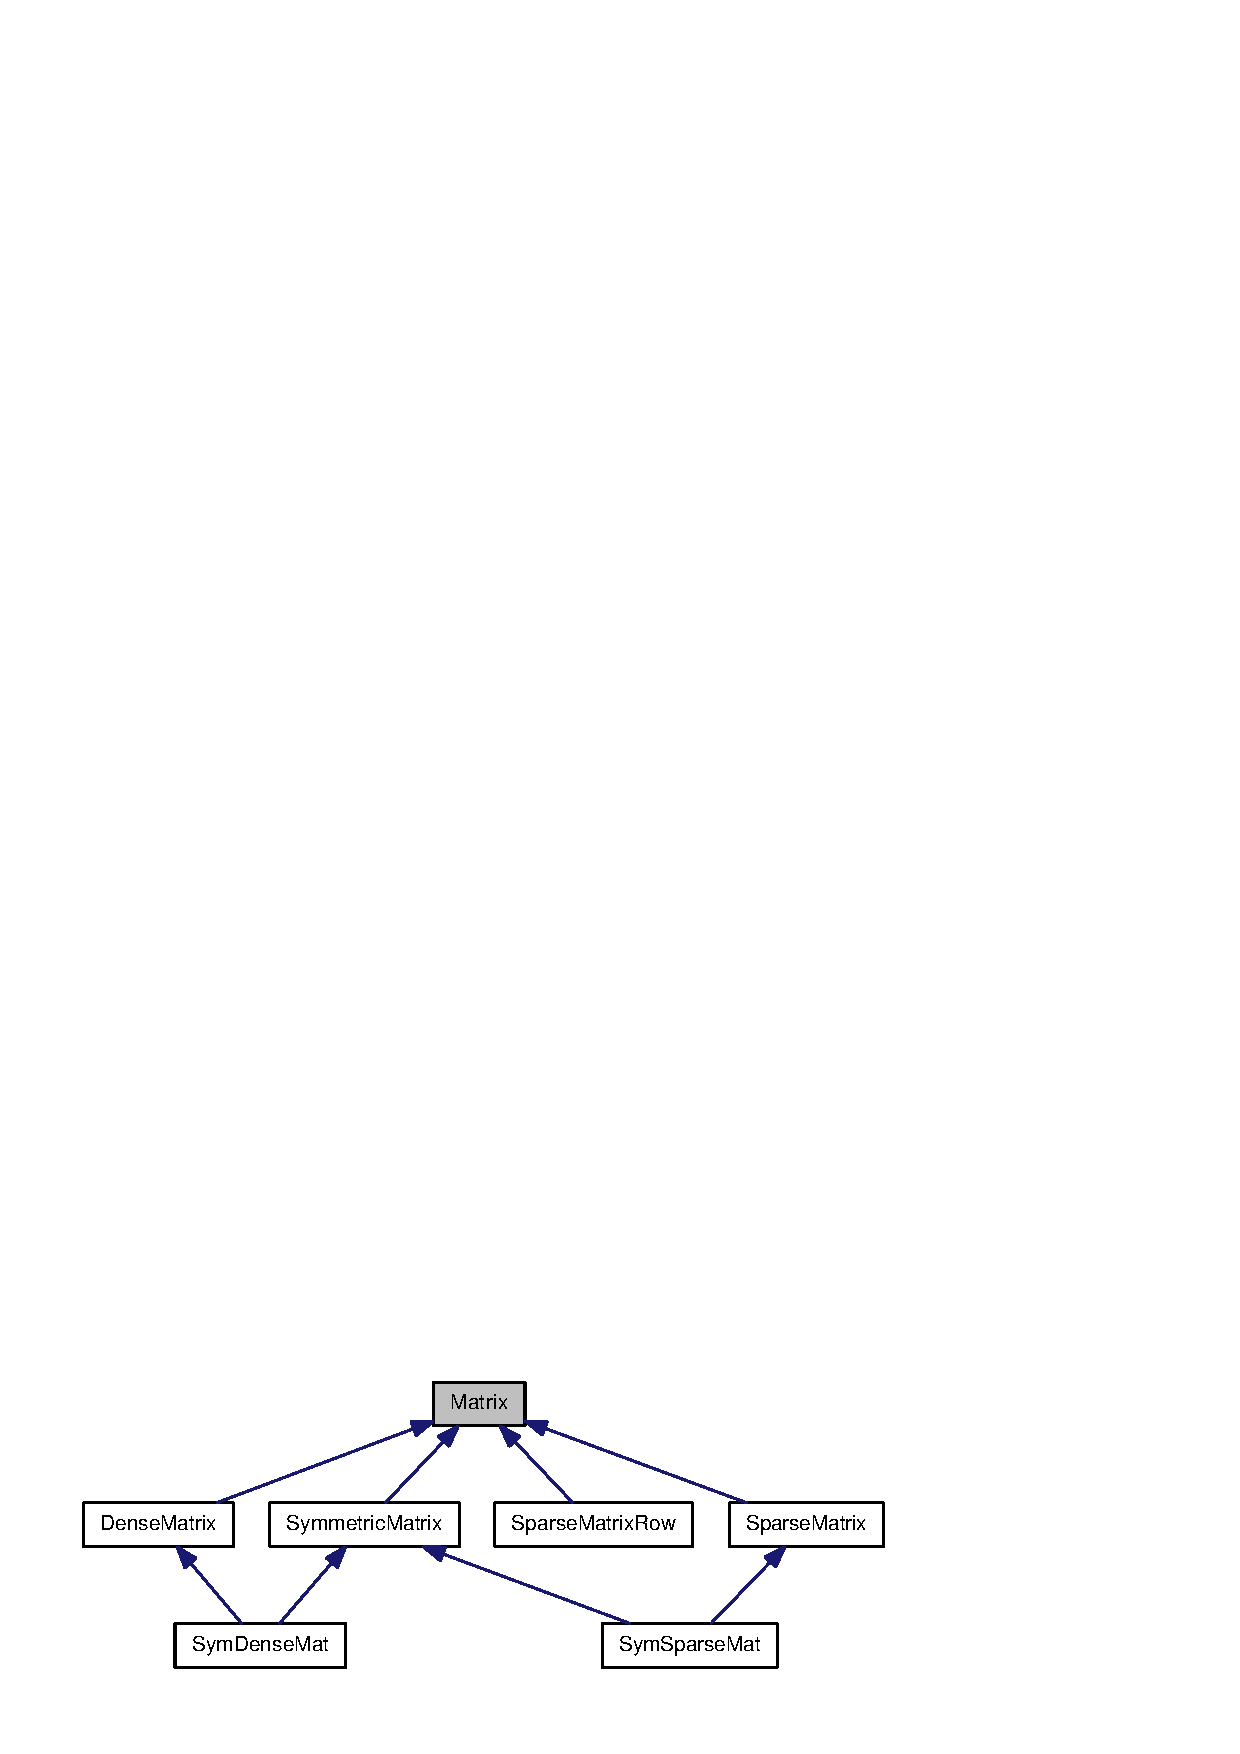
\includegraphics[width=400pt]{classMatrix__inherit__graph}
\end{center}
\end{figure}
\subsection*{Public Member Functions}
\begin{DoxyCompactItemize}
\item 
virtual {\bf returnValue} {\bf addToDiag} ({\bf real\_\-t} alpha)=0
\item 
virtual {\bf real\_\-t} {\bf diag} (int i) const =0
\item 
void {\bf doFreeMemory} ()
\item 
void {\bf doNotFreeMemory} ()
\item 
virtual {\bf Matrix} $\ast$ {\bf duplicate} () const =0
\item 
virtual void {\bf free} ()=0
\item 
virtual {\bf returnValue} {\bf getCol} (int cNum, const {\bf Indexlist} $\ast$const irows, {\bf real\_\-t} alpha, {\bf real\_\-t} $\ast$col) const =0
\item 
virtual {\bf real\_\-t} {\bf getNorm} () const =0
\item 
virtual {\bf returnValue} {\bf getRow} (int rNum, const {\bf Indexlist} $\ast$const icols, {\bf real\_\-t} alpha, {\bf real\_\-t} $\ast$row) const =0
\item 
virtual {\bf real\_\-t} {\bf getRowNorm} (int rNum) const =0
\item 
virtual {\bf BooleanType} {\bf isDiag} () const =0
\item 
{\bf Matrix} ()
\item 
{\bf BooleanType} {\bf needToFreeMemory} () const 
\item 
virtual {\bf returnValue} {\bf print} () const =0
\item 
virtual {\bf returnValue} {\bf times} (int xN, {\bf real\_\-t} alpha, const {\bf real\_\-t} $\ast$x, int xLD, {\bf real\_\-t} beta, {\bf real\_\-t} $\ast$y, int yLD) const =0
\item 
virtual {\bf returnValue} {\bf times} (const {\bf Indexlist} $\ast$const irows, const {\bf Indexlist} $\ast$const icols, int xN, {\bf real\_\-t} alpha, const {\bf real\_\-t} $\ast$x, int xLD, {\bf real\_\-t} beta, {\bf real\_\-t} $\ast$y, int yLD, {\bf BooleanType} yCompr=BT\_\-TRUE) const =0
\item 
virtual {\bf returnValue} {\bf transTimes} (const {\bf Indexlist} $\ast$const irows, const {\bf Indexlist} $\ast$const icols, int xN, {\bf real\_\-t} alpha, const {\bf real\_\-t} $\ast$x, int xLD, {\bf real\_\-t} beta, {\bf real\_\-t} $\ast$y, int yLD) const =0
\item 
virtual {\bf returnValue} {\bf transTimes} (int xN, {\bf real\_\-t} alpha, const {\bf real\_\-t} $\ast$x, int xLD, {\bf real\_\-t} beta, {\bf real\_\-t} $\ast$y, int yLD) const =0
\item 
virtual {\bf $\sim$Matrix} ()
\end{DoxyCompactItemize}
\subsection*{Protected Attributes}
\begin{DoxyCompactItemize}
\item 
{\bf BooleanType} {\bf freeMemory}
\end{DoxyCompactItemize}


\subsection{Detailed Description}
Abstract base class for interfacing tailored matrix-\/vector operations. 

Abstract base matrix class. Supplies interface to matrix vector products, including products with submatrices given by (ordered) working set index lists (see {\itshape \doxyref{SubjectTo}{p.}{classSubjectTo}\/}).

\begin{DoxyAuthor}{Author}
Andreas Potschka, Christian Kirches, Hans Joachim Ferreau 
\end{DoxyAuthor}
\begin{DoxyVersion}{Version}
3.0beta 
\end{DoxyVersion}
\begin{DoxyDate}{Date}
2011 
\end{DoxyDate}


Definition at line 120 of file Matrices.hpp.



\subsection{Constructor \& Destructor Documentation}
\index{Matrix@{Matrix}!Matrix@{Matrix}}
\index{Matrix@{Matrix}!Matrix@{Matrix}}
\subsubsection[{Matrix}]{\setlength{\rightskip}{0pt plus 5cm}Matrix::Matrix (
\begin{DoxyParamCaption}
{}
\end{DoxyParamCaption}
)\hspace{0.3cm}{\ttfamily  [inline]}}\label{classMatrix_a2dba13c45127354c9f75ef576f49269b}
Default constructor. 

Definition at line 124 of file Matrices.hpp.

\index{Matrix@{Matrix}!$\sim$Matrix@{$\sim$Matrix}}
\index{$\sim$Matrix@{$\sim$Matrix}!Matrix@{Matrix}}
\subsubsection[{$\sim$Matrix}]{\setlength{\rightskip}{0pt plus 5cm}virtual Matrix::$\sim$Matrix (
\begin{DoxyParamCaption}
{}
\end{DoxyParamCaption}
)\hspace{0.3cm}{\ttfamily  [inline, virtual]}}\label{classMatrix_ac8d10e89f7b47ab95a341d70df651554}
Destructor. 

Definition at line 127 of file Matrices.hpp.



\subsection{Member Function Documentation}
\index{Matrix@{Matrix}!addToDiag@{addToDiag}}
\index{addToDiag@{addToDiag}!Matrix@{Matrix}}
\subsubsection[{addToDiag}]{\setlength{\rightskip}{0pt plus 5cm}virtual {\bf returnValue} Matrix::addToDiag (
\begin{DoxyParamCaption}
\item[{{\bf real\_\-t}}]{alpha}
\end{DoxyParamCaption}
)\hspace{0.3cm}{\ttfamily  [pure virtual]}}\label{classMatrix_a7ee8d1b4ef0d5d5fb34342ea1889382f}
Adds given offset to diagonal of matrix. \begin{DoxyReturn}{Returns}
SUCCESSFUL\_\-RETURN \par
 RET\_\-NO\_\-DIAGONAL\_\-AVAILABLE 
\end{DoxyReturn}

\begin{DoxyParams}{Parameters}
{\em alpha} & Diagonal offset. \\
\hline
\end{DoxyParams}


Implemented in {\bf DenseMatrix} \doxyref{}{p.}{classDenseMatrix_ac901971278139a1413ff75d6106aa43b}, {\bf SparseMatrix} \doxyref{}{p.}{classSparseMatrix_a11500e9368167d4c0643fe0cebf2ccd6}, and {\bf SparseMatrixRow} \doxyref{}{p.}{classSparseMatrixRow_a6feb397255c49e09d2cb25b2b5bef57d}.

\index{Matrix@{Matrix}!diag@{diag}}
\index{diag@{diag}!Matrix@{Matrix}}
\subsubsection[{diag}]{\setlength{\rightskip}{0pt plus 5cm}virtual {\bf real\_\-t} Matrix::diag (
\begin{DoxyParamCaption}
\item[{int}]{i}
\end{DoxyParamCaption}
) const\hspace{0.3cm}{\ttfamily  [pure virtual]}}\label{classMatrix_ab78435722398170cb87b0eb9650d8ca1}
Returns i-\/th diagonal entry. \begin{DoxyReturn}{Returns}
i-\/th diagonal entry 
\end{DoxyReturn}

\begin{DoxyParams}{Parameters}
{\em i} & Index. \\
\hline
\end{DoxyParams}


Implemented in {\bf DenseMatrix} \doxyref{}{p.}{classDenseMatrix_ae0a1610915e180022f5e2161363be6ae}, {\bf SparseMatrix} \doxyref{}{p.}{classSparseMatrix_aa0137c38f1856b5b0fbc8a555171a7e6}, and {\bf SparseMatrixRow} \doxyref{}{p.}{classSparseMatrixRow_a2d7a602f21ac2221d60a4a10c06061b5}.

\index{Matrix@{Matrix}!doFreeMemory@{doFreeMemory}}
\index{doFreeMemory@{doFreeMemory}!Matrix@{Matrix}}
\subsubsection[{doFreeMemory}]{\setlength{\rightskip}{0pt plus 5cm}void Matrix::doFreeMemory (
\begin{DoxyParamCaption}
{}
\end{DoxyParamCaption}
)\hspace{0.3cm}{\ttfamily  [inline]}}\label{classMatrix_a9b1c0fc70cad1b88d6e6ab960bda478d}
Enables de-\/allocation of internal memory. 

Definition at line 242 of file Matrices.hpp.

\index{Matrix@{Matrix}!doNotFreeMemory@{doNotFreeMemory}}
\index{doNotFreeMemory@{doNotFreeMemory}!Matrix@{Matrix}}
\subsubsection[{doNotFreeMemory}]{\setlength{\rightskip}{0pt plus 5cm}void Matrix::doNotFreeMemory (
\begin{DoxyParamCaption}
{}
\end{DoxyParamCaption}
)\hspace{0.3cm}{\ttfamily  [inline]}}\label{classMatrix_a1a25e70b54e2101eb2d0c2b8a26c3d97}
Disables de-\/allocation of internal memory. 

Definition at line 245 of file Matrices.hpp.

\index{Matrix@{Matrix}!duplicate@{duplicate}}
\index{duplicate@{duplicate}!Matrix@{Matrix}}
\subsubsection[{duplicate}]{\setlength{\rightskip}{0pt plus 5cm}virtual {\bf Matrix}$\ast$ Matrix::duplicate (
\begin{DoxyParamCaption}
{}
\end{DoxyParamCaption}
) const\hspace{0.3cm}{\ttfamily  [pure virtual]}}\label{classMatrix_abf41d80f7392e9d63e9b2fa4b822d3b9}
Returns a deep-\/copy of the \doxyref{Matrix}{p.}{classMatrix} object. \begin{DoxyReturn}{Returns}
Deep-\/copy of \doxyref{Matrix}{p.}{classMatrix} object 
\end{DoxyReturn}


Implemented in {\bf DenseMatrix} \doxyref{}{p.}{classDenseMatrix_af914e214e10c8f9731da75e605dae3ff}, {\bf SymDenseMat} \doxyref{}{p.}{classSymDenseMat_af9544d2c52d356e2830e2d7dc65d9b2d}, {\bf SparseMatrix} \doxyref{}{p.}{classSparseMatrix_a70730929e8ffab371a520574d3afa2e0}, {\bf SparseMatrixRow} \doxyref{}{p.}{classSparseMatrixRow_afd8b02e3332e03dc702b9d8c12dbc4a8}, and {\bf SymSparseMat} \doxyref{}{p.}{classSymSparseMat_af125b7a9ba07555c7b6930b21637cc87}.

\index{Matrix@{Matrix}!free@{free}}
\index{free@{free}!Matrix@{Matrix}}
\subsubsection[{free}]{\setlength{\rightskip}{0pt plus 5cm}virtual void Matrix::free (
\begin{DoxyParamCaption}
{}
\end{DoxyParamCaption}
)\hspace{0.3cm}{\ttfamily  [pure virtual]}}\label{classMatrix_ae13ca77389c2eae7b3eba79cb9fefecb}
Frees all internal memory. 

Implemented in {\bf DenseMatrix} \doxyref{}{p.}{classDenseMatrix_acce63266bde8d6fd4a6c31a78c5e49e8}, {\bf SparseMatrix} \doxyref{}{p.}{classSparseMatrix_a79d5aeb24f1b1184b9fb798144999ea2}, and {\bf SparseMatrixRow} \doxyref{}{p.}{classSparseMatrixRow_a5295955ae17b29db89b8fc2607bab8c8}.

\index{Matrix@{Matrix}!getCol@{getCol}}
\index{getCol@{getCol}!Matrix@{Matrix}}
\subsubsection[{getCol}]{\setlength{\rightskip}{0pt plus 5cm}virtual {\bf returnValue} Matrix::getCol (
\begin{DoxyParamCaption}
\item[{int}]{cNum, }
\item[{const {\bf Indexlist} $\ast$const}]{irows, }
\item[{{\bf real\_\-t}}]{alpha, }
\item[{{\bf real\_\-t} $\ast$}]{col}
\end{DoxyParamCaption}
) const\hspace{0.3cm}{\ttfamily  [pure virtual]}}\label{classMatrix_a7b9f4ce0fe8c2efc34503bb260383d2c}
Retrieve indexed entries of matrix column multiplied by alpha. \begin{DoxyReturn}{Returns}
SUCCESSFUL\_\-RETURN 
\end{DoxyReturn}

\begin{DoxyParams}{Parameters}
{\em cNum} & Column number. \\
\hline
{\em irows} & Index list specifying rows. \\
\hline
{\em alpha} & Scalar factor. \\
\hline
{\em col} & Output column vector. \\
\hline
\end{DoxyParams}


Implemented in {\bf DenseMatrix} \doxyref{}{p.}{classDenseMatrix_a01b2a8928dc594099f430b4d4998ec4d}, {\bf SparseMatrix} \doxyref{}{p.}{classSparseMatrix_ad345ec5f06b26265bd32bb8b845862ae}, and {\bf SparseMatrixRow} \doxyref{}{p.}{classSparseMatrixRow_a0eda7784ab3fc69e83d5ffb60be7dee9}.

\index{Matrix@{Matrix}!getNorm@{getNorm}}
\index{getNorm@{getNorm}!Matrix@{Matrix}}
\subsubsection[{getNorm}]{\setlength{\rightskip}{0pt plus 5cm}virtual {\bf real\_\-t} Matrix::getNorm (
\begin{DoxyParamCaption}
{}
\end{DoxyParamCaption}
) const\hspace{0.3cm}{\ttfamily  [pure virtual]}}\label{classMatrix_a1cb0da3d4cf9b7c4ae21efbc05f66556}
Get the two-\/norm of the matrix \begin{DoxyReturn}{Returns}
Two-\/norm of the matrix 
\end{DoxyReturn}


Implemented in {\bf DenseMatrix} \doxyref{}{p.}{classDenseMatrix_a9e1514390cd82704505b9fa34426f7cf}, {\bf SparseMatrix} \doxyref{}{p.}{classSparseMatrix_ab42c250f99b88c40fe8e6abcb9047865}, and {\bf SparseMatrixRow} \doxyref{}{p.}{classSparseMatrixRow_adcdb1c467c3b038453499a045f1a3a01}.

\index{Matrix@{Matrix}!getRow@{getRow}}
\index{getRow@{getRow}!Matrix@{Matrix}}
\subsubsection[{getRow}]{\setlength{\rightskip}{0pt plus 5cm}virtual {\bf returnValue} Matrix::getRow (
\begin{DoxyParamCaption}
\item[{int}]{rNum, }
\item[{const {\bf Indexlist} $\ast$const}]{icols, }
\item[{{\bf real\_\-t}}]{alpha, }
\item[{{\bf real\_\-t} $\ast$}]{row}
\end{DoxyParamCaption}
) const\hspace{0.3cm}{\ttfamily  [pure virtual]}}\label{classMatrix_ab67514f6450264a6c8d55b319802099d}
Retrieve indexed entries of matrix row multiplied by alpha. \begin{DoxyReturn}{Returns}
SUCCESSFUL\_\-RETURN 
\end{DoxyReturn}

\begin{DoxyParams}{Parameters}
{\em rNum} & Row number. \\
\hline
{\em icols} & Index list specifying columns. \\
\hline
{\em alpha} & Scalar factor. \\
\hline
{\em row} & Output row vector. \\
\hline
\end{DoxyParams}


Implemented in {\bf DenseMatrix} \doxyref{}{p.}{classDenseMatrix_ab1c12481bf0f6d68776b8497058e72dc}, {\bf SparseMatrix} \doxyref{}{p.}{classSparseMatrix_ac8315e50425366ea87816e2aa5b125eb}, and {\bf SparseMatrixRow} \doxyref{}{p.}{classSparseMatrixRow_a9914ef7473337cf15da63e8550a319e2}.

\index{Matrix@{Matrix}!getRowNorm@{getRowNorm}}
\index{getRowNorm@{getRowNorm}!Matrix@{Matrix}}
\subsubsection[{getRowNorm}]{\setlength{\rightskip}{0pt plus 5cm}virtual {\bf real\_\-t} Matrix::getRowNorm (
\begin{DoxyParamCaption}
\item[{int}]{rNum}
\end{DoxyParamCaption}
) const\hspace{0.3cm}{\ttfamily  [pure virtual]}}\label{classMatrix_a44dd9bd45bd8529128b722bce60b6f42}
Get the two-\/norm of a row \begin{DoxyReturn}{Returns}
Two-\/norm of row {\itshape rNum\/} 
\end{DoxyReturn}


Implemented in {\bf DenseMatrix} \doxyref{}{p.}{classDenseMatrix_a236e8bdbfa298a30ae62740081044295}, {\bf SparseMatrix} \doxyref{}{p.}{classSparseMatrix_a034086f80de8e912cb288d64bea0ad5e}, and {\bf SparseMatrixRow} \doxyref{}{p.}{classSparseMatrixRow_ae0ff0f389e1118bfa36d1b98a5664664}.

\index{Matrix@{Matrix}!isDiag@{isDiag}}
\index{isDiag@{isDiag}!Matrix@{Matrix}}
\subsubsection[{isDiag}]{\setlength{\rightskip}{0pt plus 5cm}virtual {\bf BooleanType} Matrix::isDiag (
\begin{DoxyParamCaption}
{}
\end{DoxyParamCaption}
) const\hspace{0.3cm}{\ttfamily  [pure virtual]}}\label{classMatrix_a1f5595f0147658d9f79f92dd283dcbac}
Checks whether matrix is square and diagonal. \begin{DoxyReturn}{Returns}
BT\_\-TRUE iff matrix is square and diagonal; \par
 BT\_\-FALSE otherwise. 
\end{DoxyReturn}


Implemented in {\bf DenseMatrix} \doxyref{}{p.}{classDenseMatrix_a305a842a01cf80a33ae26d96e2d981af}, {\bf SparseMatrix} \doxyref{}{p.}{classSparseMatrix_aeaaaad0a5f3ed5d2c2112a155d1b70cd}, and {\bf SparseMatrixRow} \doxyref{}{p.}{classSparseMatrixRow_a033dd6a08ab67a871afe9cc2d9ffa2ba}.

\index{Matrix@{Matrix}!needToFreeMemory@{needToFreeMemory}}
\index{needToFreeMemory@{needToFreeMemory}!Matrix@{Matrix}}
\subsubsection[{needToFreeMemory}]{\setlength{\rightskip}{0pt plus 5cm}{\bf BooleanType} Matrix::needToFreeMemory (
\begin{DoxyParamCaption}
{}
\end{DoxyParamCaption}
) const\hspace{0.3cm}{\ttfamily  [inline]}}\label{classMatrix_ac55c39a8a1a512808f0be551be8da13a}
Returns whether internal memory needs to be de-\/allocated. \begin{DoxyReturn}{Returns}
BT\_\-TRUE iff internal memory needs to be de-\/allocated, \par
 BT\_\-FALSE otherwise 
\end{DoxyReturn}


Definition at line 239 of file Matrices.hpp.

\index{Matrix@{Matrix}!print@{print}}
\index{print@{print}!Matrix@{Matrix}}
\subsubsection[{print}]{\setlength{\rightskip}{0pt plus 5cm}virtual {\bf returnValue} Matrix::print (
\begin{DoxyParamCaption}
{}
\end{DoxyParamCaption}
) const\hspace{0.3cm}{\ttfamily  [pure virtual]}}\label{classMatrix_a110943ca5fc5b30a3e8d941622a15f8f}
Prints matrix to screen. \begin{DoxyReturn}{Returns}
SUCCESSFUL\_\-RETURN \par
 RET\_\-NOT\_\-YET\_\-IMPLEMENTED 
\end{DoxyReturn}


Implemented in {\bf DenseMatrix} \doxyref{}{p.}{classDenseMatrix_a9e3568219695311edd5911df3da2696b}, {\bf SparseMatrix} \doxyref{}{p.}{classSparseMatrix_a2c4c08afbb55942698238c7a76bcbf42}, and {\bf SparseMatrixRow} \doxyref{}{p.}{classSparseMatrixRow_a45cd971f4f2cad552070c569c5a70489}.

\index{Matrix@{Matrix}!times@{times}}
\index{times@{times}!Matrix@{Matrix}}
\subsubsection[{times}]{\setlength{\rightskip}{0pt plus 5cm}virtual {\bf returnValue} Matrix::times (
\begin{DoxyParamCaption}
\item[{const {\bf Indexlist} $\ast$const}]{irows, }
\item[{const {\bf Indexlist} $\ast$const}]{icols, }
\item[{int}]{xN, }
\item[{{\bf real\_\-t}}]{alpha, }
\item[{const {\bf real\_\-t} $\ast$}]{x, }
\item[{int}]{xLD, }
\item[{{\bf real\_\-t}}]{beta, }
\item[{{\bf real\_\-t} $\ast$}]{y, }
\item[{int}]{yLD, }
\item[{{\bf BooleanType}}]{yCompr = {\ttfamily BT\_\-TRUE}}
\end{DoxyParamCaption}
) const\hspace{0.3cm}{\ttfamily  [pure virtual]}}\label{classMatrix_add63b9303590f022b4aa49278f91f605}
Evaluate matrix vector product with submatrix given by \doxyref{Indexlist}{p.}{classIndexlist}. \begin{DoxyReturn}{Returns}
SUCCESSFUL\_\-RETURN 
\end{DoxyReturn}

\begin{DoxyParams}{Parameters}
{\em irows} & Index list specifying rows. \\
\hline
{\em icols} & Index list specifying columns. \\
\hline
{\em xN} & Number of vectors to multiply. \\
\hline
{\em alpha} & Scalar factor for matrix vector product. \\
\hline
{\em x} & Input vector to be multiplied. \\
\hline
{\em xLD} & Leading dimension of input x. \\
\hline
{\em beta} & Scalar factor for y. \\
\hline
{\em y} & Output vector of results. \\
\hline
{\em yLD} & Leading dimension of output y. \\
\hline
{\em yCompr} & Compressed storage for y. \\
\hline
\end{DoxyParams}


Implemented in {\bf DenseMatrix} \doxyref{}{p.}{classDenseMatrix_a3669612de4d322926bfedc1b85e31c7f}, {\bf SparseMatrix} \doxyref{}{p.}{classSparseMatrix_a45c425e7784421aad1d2d33825a77ca0}, and {\bf SparseMatrixRow} \doxyref{}{p.}{classSparseMatrixRow_ad643b60c929d1715ec97b14447e6f23d}.

\index{Matrix@{Matrix}!times@{times}}
\index{times@{times}!Matrix@{Matrix}}
\subsubsection[{times}]{\setlength{\rightskip}{0pt plus 5cm}virtual {\bf returnValue} Matrix::times (
\begin{DoxyParamCaption}
\item[{int}]{xN, }
\item[{{\bf real\_\-t}}]{alpha, }
\item[{const {\bf real\_\-t} $\ast$}]{x, }
\item[{int}]{xLD, }
\item[{{\bf real\_\-t}}]{beta, }
\item[{{\bf real\_\-t} $\ast$}]{y, }
\item[{int}]{yLD}
\end{DoxyParamCaption}
) const\hspace{0.3cm}{\ttfamily  [pure virtual]}}\label{classMatrix_aab443ceb9e4e37d3efca65f446872dc2}
Evaluate Y=alpha$\ast$A$\ast$X + beta$\ast$Y. \begin{DoxyReturn}{Returns}
SUCCESSFUL\_\-RETURN 
\end{DoxyReturn}

\begin{DoxyParams}{Parameters}
{\em xN} & Number of vectors to multiply. \\
\hline
{\em alpha} & Scalar factor for matrix vector product. \\
\hline
{\em x} & Input vector to be multiplied. \\
\hline
{\em xLD} & Leading dimension of input x. \\
\hline
{\em beta} & Scalar factor for y. \\
\hline
{\em y} & Output vector of results. \\
\hline
{\em yLD} & Leading dimension of output y. \\
\hline
\end{DoxyParams}


Implemented in {\bf DenseMatrix} \doxyref{}{p.}{classDenseMatrix_a6200952366ece968bce82c9400377b86}, {\bf SparseMatrix} \doxyref{}{p.}{classSparseMatrix_a3a4ef477cce34f59632e3751884f1bbc}, and {\bf SparseMatrixRow} \doxyref{}{p.}{classSparseMatrixRow_aa4bea8854c08e8de61ce1fa337e4f5c1}.

\index{Matrix@{Matrix}!transTimes@{transTimes}}
\index{transTimes@{transTimes}!Matrix@{Matrix}}
\subsubsection[{transTimes}]{\setlength{\rightskip}{0pt plus 5cm}virtual {\bf returnValue} Matrix::transTimes (
\begin{DoxyParamCaption}
\item[{int}]{xN, }
\item[{{\bf real\_\-t}}]{alpha, }
\item[{const {\bf real\_\-t} $\ast$}]{x, }
\item[{int}]{xLD, }
\item[{{\bf real\_\-t}}]{beta, }
\item[{{\bf real\_\-t} $\ast$}]{y, }
\item[{int}]{yLD}
\end{DoxyParamCaption}
) const\hspace{0.3cm}{\ttfamily  [pure virtual]}}\label{classMatrix_aae760f106376a34dfaf0c168fa836d84}
Evaluate Y=alpha$\ast$A'$\ast$X + beta$\ast$Y. \begin{DoxyReturn}{Returns}
SUCCESSFUL\_\-RETURN 
\end{DoxyReturn}

\begin{DoxyParams}{Parameters}
{\em xN} & Number of vectors to multiply. \\
\hline
{\em alpha} & Scalar factor for matrix vector product. \\
\hline
{\em x} & Input vector to be multiplied. \\
\hline
{\em xLD} & Leading dimension of input x. \\
\hline
{\em beta} & Scalar factor for y. \\
\hline
{\em y} & Output vector of results. \\
\hline
{\em yLD} & Leading dimension of output y. \\
\hline
\end{DoxyParams}


Implemented in {\bf DenseMatrix} \doxyref{}{p.}{classDenseMatrix_a5011b924f44dc66be19c2606c9083d5c}, {\bf SparseMatrix} \doxyref{}{p.}{classSparseMatrix_a96ccb53539358686a34d6ef9531694ba}, and {\bf SparseMatrixRow} \doxyref{}{p.}{classSparseMatrixRow_ac1b658d2ae14bdb519fa7304e18e3aa5}.

\index{Matrix@{Matrix}!transTimes@{transTimes}}
\index{transTimes@{transTimes}!Matrix@{Matrix}}
\subsubsection[{transTimes}]{\setlength{\rightskip}{0pt plus 5cm}virtual {\bf returnValue} Matrix::transTimes (
\begin{DoxyParamCaption}
\item[{const {\bf Indexlist} $\ast$const}]{irows, }
\item[{const {\bf Indexlist} $\ast$const}]{icols, }
\item[{int}]{xN, }
\item[{{\bf real\_\-t}}]{alpha, }
\item[{const {\bf real\_\-t} $\ast$}]{x, }
\item[{int}]{xLD, }
\item[{{\bf real\_\-t}}]{beta, }
\item[{{\bf real\_\-t} $\ast$}]{y, }
\item[{int}]{yLD}
\end{DoxyParamCaption}
) const\hspace{0.3cm}{\ttfamily  [pure virtual]}}\label{classMatrix_aa84ec7c391f7478e78ffbaf4f1f5f732}
Evaluate matrix transpose vector product. \begin{DoxyReturn}{Returns}
SUCCESSFUL\_\-RETURN 
\end{DoxyReturn}

\begin{DoxyParams}{Parameters}
{\em irows} & Index list specifying rows. \\
\hline
{\em icols} & Index list specifying columns. \\
\hline
{\em xN} & Number of vectors to multiply. \\
\hline
{\em alpha} & Scalar factor for matrix vector product. \\
\hline
{\em x} & Input vector to be multiplied. \\
\hline
{\em xLD} & Leading dimension of input x. \\
\hline
{\em beta} & Scalar factor for y. \\
\hline
{\em y} & Output vector of results. \\
\hline
{\em yLD} & Leading dimension of output y. \\
\hline
\end{DoxyParams}


Implemented in {\bf DenseMatrix} \doxyref{}{p.}{classDenseMatrix_a810893d8ddfd4bfe7d115f1b773cc9e0}, {\bf SparseMatrix} \doxyref{}{p.}{classSparseMatrix_a0b0d4d6b377acf0a7cf80e9e0376c905}, and {\bf SparseMatrixRow} \doxyref{}{p.}{classSparseMatrixRow_af4bb1e2407476f0bd19bc95e63928f0d}.



\subsection{Member Data Documentation}
\index{Matrix@{Matrix}!freeMemory@{freeMemory}}
\index{freeMemory@{freeMemory}!Matrix@{Matrix}}
\subsubsection[{freeMemory}]{\setlength{\rightskip}{0pt plus 5cm}{\bf BooleanType} {\bf Matrix::freeMemory}\hspace{0.3cm}{\ttfamily  [protected]}}\label{classMatrix_a4589bd2bde0875fe3ac82f1f97684c67}
Indicating whether internal memory needs to be de-\/allocated. 

Definition at line 245 of file Matrices.hpp.



The documentation for this class was generated from the following file:\begin{DoxyCompactItemize}
\item 
{\bf Matrices.hpp}\end{DoxyCompactItemize}

\section{ros::message\_\-traits::MD5Sum$<$ ::localized\_\-RMLD::rmld\_\-msg\_\-$<$ ContainerAllocator $>$ $>$ Struct Template Reference}
\label{structros_1_1message__traits_1_1MD5Sum_3_01_1_1localized__RMLD_1_1rmld__msg___3_01ContainerAllocator_01_4_01_4}\index{ros::message\_\-traits::MD5Sum$<$ ::localized\_\-RMLD::rmld\_\-msg\_\-$<$ ContainerAllocator $>$ $>$@{ros::message\_\-traits::MD5Sum$<$ ::localized\_\-RMLD::rmld\_\-msg\_\-$<$ ContainerAllocator $>$ $>$}}


{\ttfamily \#include $<$rmld\_\-msg.h$>$}

\subsection*{Static Public Member Functions}
\begin{DoxyCompactItemize}
\item 
static const char $\ast$ {\bf value} ()
\item 
static const char $\ast$ {\bf value} (const ::{\bf localized\_\-RMLD::rmld\_\-msg\_\-}$<$ ContainerAllocator $>$ \&)
\end{DoxyCompactItemize}
\subsection*{Static Public Attributes}
\begin{DoxyCompactItemize}
\item 
static const uint64\_\-t {\bf static\_\-value1} = 0x2d0ddf2bb2d78ac3ULL
\item 
static const uint64\_\-t {\bf static\_\-value2} = 0x56fd7ceb54e858a8ULL
\end{DoxyCompactItemize}


\subsection{Detailed Description}
\subsubsection*{template$<$class ContainerAllocator$>$struct ros::message\_\-traits::MD5Sum$<$ ::localized\_\-RMLD::rmld\_\-msg\_\-$<$ ContainerAllocator $>$ $>$}



Definition at line 171 of file rmld\_\-msg.h.



\subsection{Member Function Documentation}
\index{ros::message\_\-traits::MD5Sum$<$ ::localized\_\-RMLD::rmld\_\-msg\_\-$<$ ContainerAllocator $>$ $>$@{ros::message\_\-traits::MD5Sum$<$ ::localized\_\-RMLD::rmld\_\-msg\_\-$<$ ContainerAllocator $>$ $>$}!value@{value}}
\index{value@{value}!ros::message_traits::MD5Sum< ::localized_RMLD::rmld_msg_< ContainerAllocator > >@{ros::message\_\-traits::MD5Sum$<$ ::localized\_\-RMLD::rmld\_\-msg\_\-$<$ ContainerAllocator $>$ $>$}}
\subsubsection[{value}]{\setlength{\rightskip}{0pt plus 5cm}template$<$class ContainerAllocator $>$ static const char$\ast$ ros::message\_\-traits::MD5Sum$<$ ::{\bf localized\_\-RMLD::rmld\_\-msg\_\-}$<$ ContainerAllocator $>$ $>$::value (
\begin{DoxyParamCaption}
{}
\end{DoxyParamCaption}
)\hspace{0.3cm}{\ttfamily  [inline, static]}}\label{structros_1_1message__traits_1_1MD5Sum_3_01_1_1localized__RMLD_1_1rmld__msg___3_01ContainerAllocator_01_4_01_4_ac387b06ca714a6cb3d16159d864b7442}


Definition at line 172 of file rmld\_\-msg.h.

\index{ros::message\_\-traits::MD5Sum$<$ ::localized\_\-RMLD::rmld\_\-msg\_\-$<$ ContainerAllocator $>$ $>$@{ros::message\_\-traits::MD5Sum$<$ ::localized\_\-RMLD::rmld\_\-msg\_\-$<$ ContainerAllocator $>$ $>$}!value@{value}}
\index{value@{value}!ros::message_traits::MD5Sum< ::localized_RMLD::rmld_msg_< ContainerAllocator > >@{ros::message\_\-traits::MD5Sum$<$ ::localized\_\-RMLD::rmld\_\-msg\_\-$<$ ContainerAllocator $>$ $>$}}
\subsubsection[{value}]{\setlength{\rightskip}{0pt plus 5cm}template$<$class ContainerAllocator $>$ static const char$\ast$ ros::message\_\-traits::MD5Sum$<$ ::{\bf localized\_\-RMLD::rmld\_\-msg\_\-}$<$ ContainerAllocator $>$ $>$::value (
\begin{DoxyParamCaption}
\item[{const ::{\bf localized\_\-RMLD::rmld\_\-msg\_\-}$<$ ContainerAllocator $>$ \&}]{}
\end{DoxyParamCaption}
)\hspace{0.3cm}{\ttfamily  [inline, static]}}\label{structros_1_1message__traits_1_1MD5Sum_3_01_1_1localized__RMLD_1_1rmld__msg___3_01ContainerAllocator_01_4_01_4_a16a332d990bc7dd99c4939b308f6098f}


Definition at line 177 of file rmld\_\-msg.h.



\subsection{Member Data Documentation}
\index{ros::message\_\-traits::MD5Sum$<$ ::localized\_\-RMLD::rmld\_\-msg\_\-$<$ ContainerAllocator $>$ $>$@{ros::message\_\-traits::MD5Sum$<$ ::localized\_\-RMLD::rmld\_\-msg\_\-$<$ ContainerAllocator $>$ $>$}!static\_\-value1@{static\_\-value1}}
\index{static\_\-value1@{static\_\-value1}!ros::message_traits::MD5Sum< ::localized_RMLD::rmld_msg_< ContainerAllocator > >@{ros::message\_\-traits::MD5Sum$<$ ::localized\_\-RMLD::rmld\_\-msg\_\-$<$ ContainerAllocator $>$ $>$}}
\subsubsection[{static\_\-value1}]{\setlength{\rightskip}{0pt plus 5cm}template$<$class ContainerAllocator $>$ const uint64\_\-t ros::message\_\-traits::MD5Sum$<$ ::{\bf localized\_\-RMLD::rmld\_\-msg\_\-}$<$ ContainerAllocator $>$ $>$::{\bf static\_\-value1} = 0x2d0ddf2bb2d78ac3ULL\hspace{0.3cm}{\ttfamily  [static]}}\label{structros_1_1message__traits_1_1MD5Sum_3_01_1_1localized__RMLD_1_1rmld__msg___3_01ContainerAllocator_01_4_01_4_a467e4860611225913f67cdd0792b485f}


Definition at line 178 of file rmld\_\-msg.h.

\index{ros::message\_\-traits::MD5Sum$<$ ::localized\_\-RMLD::rmld\_\-msg\_\-$<$ ContainerAllocator $>$ $>$@{ros::message\_\-traits::MD5Sum$<$ ::localized\_\-RMLD::rmld\_\-msg\_\-$<$ ContainerAllocator $>$ $>$}!static\_\-value2@{static\_\-value2}}
\index{static\_\-value2@{static\_\-value2}!ros::message_traits::MD5Sum< ::localized_RMLD::rmld_msg_< ContainerAllocator > >@{ros::message\_\-traits::MD5Sum$<$ ::localized\_\-RMLD::rmld\_\-msg\_\-$<$ ContainerAllocator $>$ $>$}}
\subsubsection[{static\_\-value2}]{\setlength{\rightskip}{0pt plus 5cm}template$<$class ContainerAllocator $>$ const uint64\_\-t ros::message\_\-traits::MD5Sum$<$ ::{\bf localized\_\-RMLD::rmld\_\-msg\_\-}$<$ ContainerAllocator $>$ $>$::{\bf static\_\-value2} = 0x56fd7ceb54e858a8ULL\hspace{0.3cm}{\ttfamily  [static]}}\label{structros_1_1message__traits_1_1MD5Sum_3_01_1_1localized__RMLD_1_1rmld__msg___3_01ContainerAllocator_01_4_01_4_a5f6394273bd57904f5198dbb8792be23}


Definition at line 179 of file rmld\_\-msg.h.



The documentation for this struct was generated from the following file:\begin{DoxyCompactItemize}
\item 
{\bf rmld\_\-msg.h}\end{DoxyCompactItemize}

\section{MessageHandling Class Reference}
\label{classMessageHandling}\index{MessageHandling@{MessageHandling}}


Handles all kind of error messages, warnings and other information.  




{\ttfamily \#include $<$MessageHandling.hpp$>$}

\subsection*{Classes}
\begin{DoxyCompactItemize}
\item 
struct {\bf ReturnValueList}
\begin{DoxyCompactList}\small\item\em Data structure for entries in global message list. \end{DoxyCompactList}\end{DoxyCompactItemize}
\subsection*{Public Member Functions}
\begin{DoxyCompactItemize}
\item 
int {\bf getErrorCount} () const 
\item 
{\bf VisibilityStatus} {\bf getErrorVisibilityStatus} () const 
\item 
{\bf VisibilityStatus} {\bf getInfoVisibilityStatus} () const 
\item 
FILE $\ast$ {\bf getOutputFile} () const 
\item 
{\bf VisibilityStatus} {\bf getWarningVisibilityStatus} () const 
\item 
{\bf returnValue} {\bf listAllMessages} ()
\item 
{\bf MessageHandling} (FILE $\ast$\_\-outputFile)
\item 
{\bf MessageHandling} (FILE $\ast$\_\-outputFile, {\bf VisibilityStatus} \_\-errorVisibility, {\bf VisibilityStatus} \_\-warningVisibility, {\bf VisibilityStatus} \_\-infoVisibility)
\item 
{\bf MessageHandling} (const {\bf MessageHandling} \&rhs)
\item 
{\bf MessageHandling} ()
\item 
{\bf MessageHandling} ({\bf VisibilityStatus} \_\-errorVisibility, {\bf VisibilityStatus} \_\-warningVisibility, {\bf VisibilityStatus} \_\-infoVisibility)
\item 
{\bf MessageHandling} \& {\bf operator=} (const {\bf MessageHandling} \&rhs)
\item 
{\bf returnValue} {\bf reset} ()
\item 
{\bf returnValue} {\bf setErrorCount} (int \_\-errorCount)
\item 
void {\bf setErrorVisibilityStatus} ({\bf VisibilityStatus} \_\-errorVisibility)
\item 
void {\bf setInfoVisibilityStatus} ({\bf VisibilityStatus} \_\-infoVisibility)
\item 
void {\bf setOutputFile} (FILE $\ast$\_\-outputFile)
\item 
void {\bf setWarningVisibilityStatus} ({\bf VisibilityStatus} \_\-warningVisibility)
\item 
{\bf returnValue} {\bf throwError} ({\bf returnValue} Enumber, const char $\ast$additionaltext, const char $\ast$functionname, const char $\ast$filename, const unsigned long linenumber, {\bf VisibilityStatus} localVisibilityStatus)
\item 
{\bf returnValue} {\bf throwInfo} ({\bf returnValue} Inumber, const char $\ast$additionaltext, const char $\ast$functionname, const char $\ast$filename, const unsigned long linenumber, {\bf VisibilityStatus} localVisibilityStatus)
\item 
{\bf returnValue} {\bf throwWarning} ({\bf returnValue} Wnumber, const char $\ast$additionaltext, const char $\ast$functionname, const char $\ast$filename, const unsigned long linenumber, {\bf VisibilityStatus} localVisibilityStatus)
\item 
{\bf $\sim$MessageHandling} ()
\end{DoxyCompactItemize}
\subsection*{Static Public Member Functions}
\begin{DoxyCompactItemize}
\item 
static const char $\ast$ {\bf getErrorCodeMessage} (const {\bf returnValue} \_\-returnValue)
\end{DoxyCompactItemize}
\subsection*{Protected Member Functions}
\begin{DoxyCompactItemize}
\item 
{\bf returnValue} {\bf throwMessage} ({\bf returnValue} RETnumber, const char $\ast$additionaltext, const char $\ast$functionname, const char $\ast$filename, const unsigned long linenumber, {\bf VisibilityStatus} localVisibilityStatus, const char $\ast$RETstring)
\end{DoxyCompactItemize}
\subsection*{Protected Attributes}
\begin{DoxyCompactItemize}
\item 
int {\bf errorCount}
\item 
{\bf VisibilityStatus} {\bf errorVisibility}
\item 
{\bf VisibilityStatus} {\bf infoVisibility}
\item 
FILE $\ast$ {\bf outputFile}
\item 
{\bf VisibilityStatus} {\bf warningVisibility}
\end{DoxyCompactItemize}


\subsection{Detailed Description}
Handles all kind of error messages, warnings and other information. 

This class handles all kinds of messages (errors, warnings, infos) initiated by qpOASES modules and stores the correspoding global preferences.

\begin{DoxyAuthor}{Author}
Hans Joachim Ferreau (special thanks to Leonard Wirsching) 
\end{DoxyAuthor}
\begin{DoxyVersion}{Version}
3.0beta 
\end{DoxyVersion}
\begin{DoxyDate}{Date}
2007-\/2012 
\end{DoxyDate}


Definition at line 217 of file MessageHandling.hpp.



\subsection{Constructor \& Destructor Documentation}
\index{MessageHandling@{MessageHandling}!MessageHandling@{MessageHandling}}
\index{MessageHandling@{MessageHandling}!MessageHandling@{MessageHandling}}
\subsubsection[{MessageHandling}]{\setlength{\rightskip}{0pt plus 5cm}MessageHandling::MessageHandling (
\begin{DoxyParamCaption}
{}
\end{DoxyParamCaption}
)}\label{classMessageHandling_a58a64d6d798a87ed2f83092e28e7ee8b}
Default constructor. 

Definition at line 207 of file MessageHandling.cpp.

\index{MessageHandling@{MessageHandling}!MessageHandling@{MessageHandling}}
\index{MessageHandling@{MessageHandling}!MessageHandling@{MessageHandling}}
\subsubsection[{MessageHandling}]{\setlength{\rightskip}{0pt plus 5cm}MessageHandling::MessageHandling (
\begin{DoxyParamCaption}
\item[{FILE $\ast$}]{\_\-outputFile}
\end{DoxyParamCaption}
)}\label{classMessageHandling_af5fea91daefd158b856a091fd5dbdae4}
Constructor which takes the desired output file. 
\begin{DoxyParams}{Parameters}
{\em \_\-outputFile} & Output file. \\
\hline
\end{DoxyParams}


Definition at line 220 of file MessageHandling.cpp.

\index{MessageHandling@{MessageHandling}!MessageHandling@{MessageHandling}}
\index{MessageHandling@{MessageHandling}!MessageHandling@{MessageHandling}}
\subsubsection[{MessageHandling}]{\setlength{\rightskip}{0pt plus 5cm}MessageHandling::MessageHandling (
\begin{DoxyParamCaption}
\item[{{\bf VisibilityStatus}}]{\_\-errorVisibility, }
\item[{{\bf VisibilityStatus}}]{\_\-warningVisibility, }
\item[{{\bf VisibilityStatus}}]{\_\-infoVisibility}
\end{DoxyParamCaption}
)}\label{classMessageHandling_a65bf868c3aab4d7a29f9d61f235b65e4}
Constructor which takes the desired visibility states. 
\begin{DoxyParams}{Parameters}
{\em \_\-errorVisibility} & Visibility status for error messages. \\
\hline
{\em \_\-warningVisibility} & Visibility status for warning messages. \\
\hline
{\em \_\-infoVisibility} & Visibility status for info messages. \\
\hline
\end{DoxyParams}


Definition at line 233 of file MessageHandling.cpp.

\index{MessageHandling@{MessageHandling}!MessageHandling@{MessageHandling}}
\index{MessageHandling@{MessageHandling}!MessageHandling@{MessageHandling}}
\subsubsection[{MessageHandling}]{\setlength{\rightskip}{0pt plus 5cm}MessageHandling::MessageHandling (
\begin{DoxyParamCaption}
\item[{FILE $\ast$}]{\_\-outputFile, }
\item[{{\bf VisibilityStatus}}]{\_\-errorVisibility, }
\item[{{\bf VisibilityStatus}}]{\_\-warningVisibility, }
\item[{{\bf VisibilityStatus}}]{\_\-infoVisibility}
\end{DoxyParamCaption}
)}\label{classMessageHandling_aedfc5f9079f5dd454a13700e13e029d7}
Constructor which takes the desired output file and desired visibility states. 
\begin{DoxyParams}{Parameters}
{\em \_\-outputFile} & Output file. \\
\hline
{\em \_\-errorVisibility} & Visibility status for error messages. \\
\hline
{\em \_\-warningVisibility} & Visibility status for warning messages. \\
\hline
{\em \_\-infoVisibility} & Visibility status for info messages. \\
\hline
\end{DoxyParams}


Definition at line 249 of file MessageHandling.cpp.

\index{MessageHandling@{MessageHandling}!MessageHandling@{MessageHandling}}
\index{MessageHandling@{MessageHandling}!MessageHandling@{MessageHandling}}
\subsubsection[{MessageHandling}]{\setlength{\rightskip}{0pt plus 5cm}MessageHandling::MessageHandling (
\begin{DoxyParamCaption}
\item[{const {\bf MessageHandling} \&}]{rhs}
\end{DoxyParamCaption}
)}\label{classMessageHandling_a9702e58c2dd05e674fc47ed44f92ff30}
Copy constructor (deep copy). 
\begin{DoxyParams}{Parameters}
{\em rhs} & Rhs object. \\
\hline
\end{DoxyParams}


Definition at line 268 of file MessageHandling.cpp.

\index{MessageHandling@{MessageHandling}!$\sim$MessageHandling@{$\sim$MessageHandling}}
\index{$\sim$MessageHandling@{$\sim$MessageHandling}!MessageHandling@{MessageHandling}}
\subsubsection[{$\sim$MessageHandling}]{\setlength{\rightskip}{0pt plus 5cm}MessageHandling::$\sim$MessageHandling (
\begin{DoxyParamCaption}
{}
\end{DoxyParamCaption}
)}\label{classMessageHandling_a732439c8915c726c29833a335fb60ae7}
Destructor. 

Definition at line 282 of file MessageHandling.cpp.



\subsection{Member Function Documentation}
\index{MessageHandling@{MessageHandling}!getErrorCodeMessage@{getErrorCodeMessage}}
\index{getErrorCodeMessage@{getErrorCodeMessage}!MessageHandling@{MessageHandling}}
\subsubsection[{getErrorCodeMessage}]{\setlength{\rightskip}{0pt plus 5cm}const char $\ast$ MessageHandling::getErrorCodeMessage (
\begin{DoxyParamCaption}
\item[{const {\bf returnValue}}]{\_\-returnValue}
\end{DoxyParamCaption}
)\hspace{0.3cm}{\ttfamily  [static]}}\label{classMessageHandling_aa6107f3844b0d91478daec1301620560}
Provides message text corresponding to given {\itshape returnValue\/}. \begin{DoxyReturn}{Returns}
String containing message text. 
\end{DoxyReturn}


Definition at line 530 of file MessageHandling.cpp.

\index{MessageHandling@{MessageHandling}!getErrorCount@{getErrorCount}}
\index{getErrorCount@{getErrorCount}!MessageHandling@{MessageHandling}}
\subsubsection[{getErrorCount}]{\setlength{\rightskip}{0pt plus 5cm}int MessageHandling::getErrorCount (
\begin{DoxyParamCaption}
{}
\end{DoxyParamCaption}
) const\hspace{0.3cm}{\ttfamily  [inline]}}\label{classMessageHandling_a9b5aaeda8506e708c78aa1e4ae0a5ae1}
Returns error count value. \begin{DoxyReturn}{Returns}
Error count value. 
\end{DoxyReturn}
\index{MessageHandling@{MessageHandling}!getErrorVisibilityStatus@{getErrorVisibilityStatus}}
\index{getErrorVisibilityStatus@{getErrorVisibilityStatus}!MessageHandling@{MessageHandling}}
\subsubsection[{getErrorVisibilityStatus}]{\setlength{\rightskip}{0pt plus 5cm}{\bf VisibilityStatus} MessageHandling::getErrorVisibilityStatus (
\begin{DoxyParamCaption}
{}
\end{DoxyParamCaption}
) const\hspace{0.3cm}{\ttfamily  [inline]}}\label{classMessageHandling_ac0aa0041e157271d1a08623e795c333e}
Returns visibility status for error messages. \begin{DoxyReturn}{Returns}
Visibility status for error messages. 
\end{DoxyReturn}
\index{MessageHandling@{MessageHandling}!getInfoVisibilityStatus@{getInfoVisibilityStatus}}
\index{getInfoVisibilityStatus@{getInfoVisibilityStatus}!MessageHandling@{MessageHandling}}
\subsubsection[{getInfoVisibilityStatus}]{\setlength{\rightskip}{0pt plus 5cm}{\bf VisibilityStatus} MessageHandling::getInfoVisibilityStatus (
\begin{DoxyParamCaption}
{}
\end{DoxyParamCaption}
) const\hspace{0.3cm}{\ttfamily  [inline]}}\label{classMessageHandling_ae9eaf40fc69f2f8e339d59fcba54c8f3}
Returns visibility status for info messages. \begin{DoxyReturn}{Returns}
Visibility status for info messages. 
\end{DoxyReturn}
\index{MessageHandling@{MessageHandling}!getOutputFile@{getOutputFile}}
\index{getOutputFile@{getOutputFile}!MessageHandling@{MessageHandling}}
\subsubsection[{getOutputFile}]{\setlength{\rightskip}{0pt plus 5cm}FILE$\ast$ MessageHandling::getOutputFile (
\begin{DoxyParamCaption}
{}
\end{DoxyParamCaption}
) const\hspace{0.3cm}{\ttfamily  [inline]}}\label{classMessageHandling_a5bebdda93df04994caced3c553594e3d}
Returns pointer to output file. \begin{DoxyReturn}{Returns}
Pointer to output file. 
\end{DoxyReturn}
\index{MessageHandling@{MessageHandling}!getWarningVisibilityStatus@{getWarningVisibilityStatus}}
\index{getWarningVisibilityStatus@{getWarningVisibilityStatus}!MessageHandling@{MessageHandling}}
\subsubsection[{getWarningVisibilityStatus}]{\setlength{\rightskip}{0pt plus 5cm}{\bf VisibilityStatus} MessageHandling::getWarningVisibilityStatus (
\begin{DoxyParamCaption}
{}
\end{DoxyParamCaption}
) const\hspace{0.3cm}{\ttfamily  [inline]}}\label{classMessageHandling_a96631494d02e2bc6db47375697de698e}
Returns visibility status for warning messages. \begin{DoxyReturn}{Returns}
Visibility status for warning messages. 
\end{DoxyReturn}
\index{MessageHandling@{MessageHandling}!listAllMessages@{listAllMessages}}
\index{listAllMessages@{listAllMessages}!MessageHandling@{MessageHandling}}
\subsubsection[{listAllMessages}]{\setlength{\rightskip}{0pt plus 5cm}{\bf returnValue} MessageHandling::listAllMessages (
\begin{DoxyParamCaption}
{}
\end{DoxyParamCaption}
)}\label{classMessageHandling_a8b6ff3603352ace1322188f156983c44}
Prints a complete list of all messages to output file. \begin{DoxyReturn}{Returns}
SUCCESSFUL\_\-RETURN 
\end{DoxyReturn}


Definition at line 399 of file MessageHandling.cpp.

\index{MessageHandling@{MessageHandling}!operator=@{operator=}}
\index{operator=@{operator=}!MessageHandling@{MessageHandling}}
\subsubsection[{operator=}]{\setlength{\rightskip}{0pt plus 5cm}{\bf MessageHandling} \& MessageHandling::operator= (
\begin{DoxyParamCaption}
\item[{const {\bf MessageHandling} \&}]{rhs}
\end{DoxyParamCaption}
)}\label{classMessageHandling_a5bdc56ea0f2ba7d70b9c47a3403692a1}
Assignment operator (deep copy). 
\begin{DoxyParams}{Parameters}
{\em rhs} & Rhs object. \\
\hline
\end{DoxyParams}


Definition at line 292 of file MessageHandling.cpp.

\index{MessageHandling@{MessageHandling}!reset@{reset}}
\index{reset@{reset}!MessageHandling@{MessageHandling}}
\subsubsection[{reset}]{\setlength{\rightskip}{0pt plus 5cm}{\bf returnValue} MessageHandling::reset (
\begin{DoxyParamCaption}
{}
\end{DoxyParamCaption}
)}\label{classMessageHandling_aee146336fc1d08ae20ea00498aee471f}
Resets all preferences to default values. \begin{DoxyReturn}{Returns}
SUCCESSFUL\_\-RETURN 
\end{DoxyReturn}


Definition at line 383 of file MessageHandling.cpp.

\index{MessageHandling@{MessageHandling}!setErrorCount@{setErrorCount}}
\index{setErrorCount@{setErrorCount}!MessageHandling@{MessageHandling}}
\subsubsection[{setErrorCount}]{\setlength{\rightskip}{0pt plus 5cm}{\bf returnValue} MessageHandling::setErrorCount (
\begin{DoxyParamCaption}
\item[{int}]{\_\-errorCount}
\end{DoxyParamCaption}
)\hspace{0.3cm}{\ttfamily  [inline]}}\label{classMessageHandling_a8e098ad6661d636e584565b58d2fe42a}
Changes error count. \begin{DoxyReturn}{Returns}
SUCCESSFUL\_\-RETURN \par
 RET\_\-INVALID\_\-ARGUMENT 
\end{DoxyReturn}

\begin{DoxyParams}{Parameters}
{\em \_\-errorCount} & New error count value. \\
\hline
\end{DoxyParams}
\index{MessageHandling@{MessageHandling}!setErrorVisibilityStatus@{setErrorVisibilityStatus}}
\index{setErrorVisibilityStatus@{setErrorVisibilityStatus}!MessageHandling@{MessageHandling}}
\subsubsection[{setErrorVisibilityStatus}]{\setlength{\rightskip}{0pt plus 5cm}void MessageHandling::setErrorVisibilityStatus (
\begin{DoxyParamCaption}
\item[{{\bf VisibilityStatus}}]{\_\-errorVisibility}
\end{DoxyParamCaption}
)\hspace{0.3cm}{\ttfamily  [inline]}}\label{classMessageHandling_a31f12baabf23d05c97e2da9dbd8adf6e}
Changes visibility status for error messages. 
\begin{DoxyParams}{Parameters}
{\em \_\-errorVisibility} & New visibility status for error messages. \\
\hline
\end{DoxyParams}
\index{MessageHandling@{MessageHandling}!setInfoVisibilityStatus@{setInfoVisibilityStatus}}
\index{setInfoVisibilityStatus@{setInfoVisibilityStatus}!MessageHandling@{MessageHandling}}
\subsubsection[{setInfoVisibilityStatus}]{\setlength{\rightskip}{0pt plus 5cm}void MessageHandling::setInfoVisibilityStatus (
\begin{DoxyParamCaption}
\item[{{\bf VisibilityStatus}}]{\_\-infoVisibility}
\end{DoxyParamCaption}
)\hspace{0.3cm}{\ttfamily  [inline]}}\label{classMessageHandling_ac1f2497e237ab552f408db52e7ba6359}
Changes visibility status for info messages. 
\begin{DoxyParams}{Parameters}
{\em \_\-infoVisibility} & New visibility status for info messages. \\
\hline
\end{DoxyParams}
\index{MessageHandling@{MessageHandling}!setOutputFile@{setOutputFile}}
\index{setOutputFile@{setOutputFile}!MessageHandling@{MessageHandling}}
\subsubsection[{setOutputFile}]{\setlength{\rightskip}{0pt plus 5cm}void MessageHandling::setOutputFile (
\begin{DoxyParamCaption}
\item[{FILE $\ast$}]{\_\-outputFile}
\end{DoxyParamCaption}
)\hspace{0.3cm}{\ttfamily  [inline]}}\label{classMessageHandling_a91cf9df3e66b84d4fb6039b39de32390}
Changes output file for messages. 
\begin{DoxyParams}{Parameters}
{\em \_\-outputFile} & New output file for messages. \\
\hline
\end{DoxyParams}
\index{MessageHandling@{MessageHandling}!setWarningVisibilityStatus@{setWarningVisibilityStatus}}
\index{setWarningVisibilityStatus@{setWarningVisibilityStatus}!MessageHandling@{MessageHandling}}
\subsubsection[{setWarningVisibilityStatus}]{\setlength{\rightskip}{0pt plus 5cm}void MessageHandling::setWarningVisibilityStatus (
\begin{DoxyParamCaption}
\item[{{\bf VisibilityStatus}}]{\_\-warningVisibility}
\end{DoxyParamCaption}
)\hspace{0.3cm}{\ttfamily  [inline]}}\label{classMessageHandling_aaa411b35b599fe59c57b94e0eb0f2728}
Changes visibility status for warning messages. 
\begin{DoxyParams}{Parameters}
{\em \_\-warningVisibility} & New visibility status for warning messages. \\
\hline
\end{DoxyParams}
\index{MessageHandling@{MessageHandling}!throwError@{throwError}}
\index{throwError@{throwError}!MessageHandling@{MessageHandling}}
\subsubsection[{throwError}]{\setlength{\rightskip}{0pt plus 5cm}{\bf returnValue} MessageHandling::throwError (
\begin{DoxyParamCaption}
\item[{{\bf returnValue}}]{Enumber, }
\item[{const char $\ast$}]{additionaltext, }
\item[{const char $\ast$}]{functionname, }
\item[{const char $\ast$}]{filename, }
\item[{const unsigned long}]{linenumber, }
\item[{{\bf VisibilityStatus}}]{localVisibilityStatus}
\end{DoxyParamCaption}
)}\label{classMessageHandling_a257d3209e0efcb245753be9d9f89e4cf}
Prints an error message(a simplified macro THROWERROR is also provided). \par
 Errors are definied as abnormal events which cause an immediate termination of the current (sub) function. Errors of a sub function should be commented by the calling function by means of a warning message (if this error does not cause an error of the calling function, either)! \begin{DoxyReturn}{Returns}
Error number returned by sub function call 
\end{DoxyReturn}

\begin{DoxyParams}{Parameters}
{\em Enumber} & Error number returned by sub function call. \\
\hline
{\em additionaltext} & Additional error text (0, if none). \\
\hline
{\em functionname} & Name of function which caused the error. \\
\hline
{\em filename} & Name of file which caused the error. \\
\hline
{\em linenumber} & Number of line which caused the error.incompatible binary file \\
\hline
{\em localVisibilityStatus} & Determines (locally) if error message can be printed to stderr. If GLOBAL visibility status of the message is set to VS\_\-HIDDEN, no message is printed, anyway! \\
\hline
\end{DoxyParams}


Definition at line 311 of file MessageHandling.cpp.

\index{MessageHandling@{MessageHandling}!throwInfo@{throwInfo}}
\index{throwInfo@{throwInfo}!MessageHandling@{MessageHandling}}
\subsubsection[{throwInfo}]{\setlength{\rightskip}{0pt plus 5cm}{\bf returnValue} MessageHandling::throwInfo (
\begin{DoxyParamCaption}
\item[{{\bf returnValue}}]{Inumber, }
\item[{const char $\ast$}]{additionaltext, }
\item[{const char $\ast$}]{functionname, }
\item[{const char $\ast$}]{filename, }
\item[{const unsigned long}]{linenumber, }
\item[{{\bf VisibilityStatus}}]{localVisibilityStatus}
\end{DoxyParamCaption}
)}\label{classMessageHandling_a57fafea776d1d7be7a36676a7396aabe}
Prints a info message (a simplified macro THROWINFO is also provided). \begin{DoxyReturn}{Returns}
Info number returned by sub function call 
\end{DoxyReturn}

\begin{DoxyParams}{Parameters}
{\em Inumber} & Info number returned by sub function call. \\
\hline
{\em additionaltext} & Additional warning text (0, if none). \\
\hline
{\em functionname} & Name of function which submitted the info. \\
\hline
{\em filename} & Name of file which submitted the info. \\
\hline
{\em linenumber} & Number of line which submitted the info. \\
\hline
{\em localVisibilityStatus} & Determines (locally) if info message can be printed to stderr. If GLOBAL visibility status of the message is set to VS\_\-HIDDEN, no message is printed, anyway! \\
\hline
\end{DoxyParams}


Definition at line 359 of file MessageHandling.cpp.

\index{MessageHandling@{MessageHandling}!throwMessage@{throwMessage}}
\index{throwMessage@{throwMessage}!MessageHandling@{MessageHandling}}
\subsubsection[{throwMessage}]{\setlength{\rightskip}{0pt plus 5cm}{\bf returnValue} MessageHandling::throwMessage (
\begin{DoxyParamCaption}
\item[{{\bf returnValue}}]{RETnumber, }
\item[{const char $\ast$}]{additionaltext, }
\item[{const char $\ast$}]{functionname, }
\item[{const char $\ast$}]{filename, }
\item[{const unsigned long}]{linenumber, }
\item[{{\bf VisibilityStatus}}]{localVisibilityStatus, }
\item[{const char $\ast$}]{RETstring}
\end{DoxyParamCaption}
)\hspace{0.3cm}{\ttfamily  [protected]}}\label{classMessageHandling_ab7eff297de539c158ed8583f2146a352}
Prints a info message to stderr (auxiliary function). \begin{DoxyReturn}{Returns}
Error/warning/info number returned by sub function call 
\end{DoxyReturn}

\begin{DoxyParams}{Parameters}
{\em RETnumber} & Error/warning/info number returned by sub function call. \\
\hline
{\em additionaltext} & Additional warning text (0, if none). \\
\hline
{\em functionname} & Name of function which caused the error/warning/info. \\
\hline
{\em filename} & Name of file which caused the error/warning/info. \\
\hline
{\em linenumber} & Number of line which caused the error/warning/info. \\
\hline
{\em localVisibilityStatus} & Determines (locally) if info message can be printed to stderr. If GLOBAL visibility status of the message is set to VS\_\-HIDDEN, no message is printed, anyway! \\
\hline
{\em RETstring} & Leading string of error/warning/info message. \\
\hline
\end{DoxyParams}


Definition at line 428 of file MessageHandling.cpp.

\index{MessageHandling@{MessageHandling}!throwWarning@{throwWarning}}
\index{throwWarning@{throwWarning}!MessageHandling@{MessageHandling}}
\subsubsection[{throwWarning}]{\setlength{\rightskip}{0pt plus 5cm}{\bf returnValue} MessageHandling::throwWarning (
\begin{DoxyParamCaption}
\item[{{\bf returnValue}}]{Wnumber, }
\item[{const char $\ast$}]{additionaltext, }
\item[{const char $\ast$}]{functionname, }
\item[{const char $\ast$}]{filename, }
\item[{const unsigned long}]{linenumber, }
\item[{{\bf VisibilityStatus}}]{localVisibilityStatus}
\end{DoxyParamCaption}
)}\label{classMessageHandling_a20916177fb0e5a55e1cc74df22e53795}
Prints a warning message (a simplified macro THROWWARNING is also provided). Warnings are definied as abnormal events which does NOT cause an immediate termination of the current (sub) function. \begin{DoxyReturn}{Returns}
Warning number returned by sub function call 
\end{DoxyReturn}

\begin{DoxyParams}{Parameters}
{\em Wnumber} & Warning number returned by sub function call. \\
\hline
{\em additionaltext} & Additional warning text (0, if none). \\
\hline
{\em functionname} & Name of function which caused the warning. \\
\hline
{\em filename} & Name of file which caused the warning. \\
\hline
{\em linenumber} & Number of line which caused the warning. \\
\hline
{\em localVisibilityStatus} & Determines (locally) if warning message can be printed to stderr. If GLOBAL visibility status of the message is set to VS\_\-HIDDEN, no message is printed, anyway! \\
\hline
\end{DoxyParams}


Definition at line 335 of file MessageHandling.cpp.



\subsection{Member Data Documentation}
\index{MessageHandling@{MessageHandling}!errorCount@{errorCount}}
\index{errorCount@{errorCount}!MessageHandling@{MessageHandling}}
\subsubsection[{errorCount}]{\setlength{\rightskip}{0pt plus 5cm}int {\bf MessageHandling::errorCount}\hspace{0.3cm}{\ttfamily  [protected]}}\label{classMessageHandling_a3ac4bf299eed3c527b021630b77eee55}
Counts number of errors (for nicer output only). 

Definition at line 407 of file MessageHandling.hpp.

\index{MessageHandling@{MessageHandling}!errorVisibility@{errorVisibility}}
\index{errorVisibility@{errorVisibility}!MessageHandling@{MessageHandling}}
\subsubsection[{errorVisibility}]{\setlength{\rightskip}{0pt plus 5cm}{\bf VisibilityStatus} {\bf MessageHandling::errorVisibility}\hspace{0.3cm}{\ttfamily  [protected]}}\label{classMessageHandling_af75a2fd3122cc2a9793c5ad491b04325}
Error messages visible? 

Definition at line 401 of file MessageHandling.hpp.

\index{MessageHandling@{MessageHandling}!infoVisibility@{infoVisibility}}
\index{infoVisibility@{infoVisibility}!MessageHandling@{MessageHandling}}
\subsubsection[{infoVisibility}]{\setlength{\rightskip}{0pt plus 5cm}{\bf VisibilityStatus} {\bf MessageHandling::infoVisibility}\hspace{0.3cm}{\ttfamily  [protected]}}\label{classMessageHandling_a6a630fa427803cf4e1e0f54d8fb14a1b}
Info messages visible? 

Definition at line 403 of file MessageHandling.hpp.

\index{MessageHandling@{MessageHandling}!outputFile@{outputFile}}
\index{outputFile@{outputFile}!MessageHandling@{MessageHandling}}
\subsubsection[{outputFile}]{\setlength{\rightskip}{0pt plus 5cm}FILE$\ast$ {\bf MessageHandling::outputFile}\hspace{0.3cm}{\ttfamily  [protected]}}\label{classMessageHandling_a2a40cbdfced701a18da281f7a4e910ee}
Output file for messages. 

Definition at line 405 of file MessageHandling.hpp.

\index{MessageHandling@{MessageHandling}!warningVisibility@{warningVisibility}}
\index{warningVisibility@{warningVisibility}!MessageHandling@{MessageHandling}}
\subsubsection[{warningVisibility}]{\setlength{\rightskip}{0pt plus 5cm}{\bf VisibilityStatus} {\bf MessageHandling::warningVisibility}\hspace{0.3cm}{\ttfamily  [protected]}}\label{classMessageHandling_af715e377af244418a8003b172c8bdf91}
Warning messages visible? 

Definition at line 402 of file MessageHandling.hpp.



The documentation for this class was generated from the following files:\begin{DoxyCompactItemize}
\item 
{\bf MessageHandling.hpp}\item 
{\bf MessageHandling.cpp}\end{DoxyCompactItemize}

\section{MyConstraintProduct Class Reference}
\label{classMyConstraintProduct}\index{MyConstraintProduct@{MyConstraintProduct}}


Example illustrating the use of the {\itshape \doxyref{ConstraintProduct}{p.}{classConstraintProduct}\/} class.  




Inheritance diagram for MyConstraintProduct:
\nopagebreak
\begin{figure}[H]
\begin{center}
\leavevmode
\includegraphics[width=152pt]{classMyConstraintProduct__inherit__graph}
\end{center}
\end{figure}
\subsection*{Public Member Functions}
\begin{DoxyCompactItemize}
\item 
{\bf MyConstraintProduct} ()
\item 
{\bf MyConstraintProduct} (int \_\-nV, int \_\-nC, {\bf real\_\-t} $\ast$\_\-A)
\item 
{\bf MyConstraintProduct} (const {\bf MyConstraintProduct} \&rhs)
\item 
virtual int {\bf operator()} (int constrIndex, const {\bf real\_\-t} $\ast$const x, {\bf real\_\-t} $\ast$const constrValue) const 
\item 
{\bf MyConstraintProduct} \& {\bf operator=} (const {\bf MyConstraintProduct} \&rhs)
\item 
virtual {\bf $\sim$MyConstraintProduct} ()
\end{DoxyCompactItemize}
\subsection*{Protected Attributes}
\begin{DoxyCompactItemize}
\item 
{\bf real\_\-t} $\ast$ {\bf A}
\item 
int {\bf nC}
\item 
int {\bf nV}
\end{DoxyCompactItemize}


\subsection{Detailed Description}
Example illustrating the use of the {\itshape \doxyref{ConstraintProduct}{p.}{classConstraintProduct}\/} class. 

Example illustrating the use of the {\itshape \doxyref{ConstraintProduct}{p.}{classConstraintProduct}\/} class.

\begin{DoxyAuthor}{Author}
Hans Joachim Ferreau 
\end{DoxyAuthor}
\begin{DoxyVersion}{Version}
3.0beta 
\end{DoxyVersion}
\begin{DoxyDate}{Date}
2007-\/2012 
\end{DoxyDate}


Definition at line 47 of file example4CP.cpp.



\subsection{Constructor \& Destructor Documentation}
\index{MyConstraintProduct@{MyConstraintProduct}!MyConstraintProduct@{MyConstraintProduct}}
\index{MyConstraintProduct@{MyConstraintProduct}!MyConstraintProduct@{MyConstraintProduct}}
\subsubsection[{MyConstraintProduct}]{\setlength{\rightskip}{0pt plus 5cm}MyConstraintProduct::MyConstraintProduct (
\begin{DoxyParamCaption}
{}
\end{DoxyParamCaption}
)\hspace{0.3cm}{\ttfamily  [inline]}}\label{classMyConstraintProduct_a670ac34e0d2147f7be90334c51c280b1}


Definition at line 50 of file example4CP.cpp.

\index{MyConstraintProduct@{MyConstraintProduct}!MyConstraintProduct@{MyConstraintProduct}}
\index{MyConstraintProduct@{MyConstraintProduct}!MyConstraintProduct@{MyConstraintProduct}}
\subsubsection[{MyConstraintProduct}]{\setlength{\rightskip}{0pt plus 5cm}MyConstraintProduct::MyConstraintProduct (
\begin{DoxyParamCaption}
\item[{int}]{\_\-nV, }
\item[{int}]{\_\-nC, }
\item[{{\bf real\_\-t} $\ast$}]{\_\-A}
\end{DoxyParamCaption}
)\hspace{0.3cm}{\ttfamily  [inline]}}\label{classMyConstraintProduct_a025e4752ea75b5ce64c21672847251b9}


Definition at line 52 of file example4CP.cpp.

\index{MyConstraintProduct@{MyConstraintProduct}!MyConstraintProduct@{MyConstraintProduct}}
\index{MyConstraintProduct@{MyConstraintProduct}!MyConstraintProduct@{MyConstraintProduct}}
\subsubsection[{MyConstraintProduct}]{\setlength{\rightskip}{0pt plus 5cm}MyConstraintProduct::MyConstraintProduct (
\begin{DoxyParamCaption}
\item[{const {\bf MyConstraintProduct} \&}]{rhs}
\end{DoxyParamCaption}
)\hspace{0.3cm}{\ttfamily  [inline]}}\label{classMyConstraintProduct_a8713cbd57754373bb7b882b18a6dda3b}


Definition at line 62 of file example4CP.cpp.

\index{MyConstraintProduct@{MyConstraintProduct}!$\sim$MyConstraintProduct@{$\sim$MyConstraintProduct}}
\index{$\sim$MyConstraintProduct@{$\sim$MyConstraintProduct}!MyConstraintProduct@{MyConstraintProduct}}
\subsubsection[{$\sim$MyConstraintProduct}]{\setlength{\rightskip}{0pt plus 5cm}virtual MyConstraintProduct::$\sim$MyConstraintProduct (
\begin{DoxyParamCaption}
{}
\end{DoxyParamCaption}
)\hspace{0.3cm}{\ttfamily  [inline, virtual]}}\label{classMyConstraintProduct_a91575bc7f737462aef210acec28b322e}


Definition at line 70 of file example4CP.cpp.



\subsection{Member Function Documentation}
\index{MyConstraintProduct@{MyConstraintProduct}!operator()@{operator()}}
\index{operator()@{operator()}!MyConstraintProduct@{MyConstraintProduct}}
\subsubsection[{operator()}]{\setlength{\rightskip}{0pt plus 5cm}virtual int MyConstraintProduct::operator() (
\begin{DoxyParamCaption}
\item[{int}]{constrIndex, }
\item[{const {\bf real\_\-t} $\ast$const}]{x, }
\item[{{\bf real\_\-t} $\ast$const}]{constrValue}
\end{DoxyParamCaption}
) const\hspace{0.3cm}{\ttfamily  [inline, virtual]}}\label{classMyConstraintProduct_ac967b02d33098635e411e6edef2ef460}
Evaluates the product of a given constraint with the current iterate. This function needs to be implemented in a derived class for the user-\/defined constraint product function. \begin{DoxyReturn}{Returns}
0: successful \par
 otherwise: not successful 
\end{DoxyReturn}


Implements {\bf ConstraintProduct} \doxyref{}{p.}{classConstraintProduct_a1da981e12cd8d7411bcdf43b827c5c1d}.



Definition at line 85 of file example4CP.cpp.

\index{MyConstraintProduct@{MyConstraintProduct}!operator=@{operator=}}
\index{operator=@{operator=}!MyConstraintProduct@{MyConstraintProduct}}
\subsubsection[{operator=}]{\setlength{\rightskip}{0pt plus 5cm}{\bf MyConstraintProduct}\& MyConstraintProduct::operator= (
\begin{DoxyParamCaption}
\item[{const {\bf MyConstraintProduct} \&}]{rhs}
\end{DoxyParamCaption}
)\hspace{0.3cm}{\ttfamily  [inline]}}\label{classMyConstraintProduct_a782959ec14624f774582d954b8ab9a70}


Definition at line 72 of file example4CP.cpp.



\subsection{Member Data Documentation}
\index{MyConstraintProduct@{MyConstraintProduct}!A@{A}}
\index{A@{A}!MyConstraintProduct@{MyConstraintProduct}}
\subsubsection[{A}]{\setlength{\rightskip}{0pt plus 5cm}{\bf real\_\-t}$\ast$ {\bf MyConstraintProduct::A}\hspace{0.3cm}{\ttfamily  [protected]}}\label{classMyConstraintProduct_a654d468b76949a46fc92d3c0fae8b8f7}


Definition at line 101 of file example4CP.cpp.

\index{MyConstraintProduct@{MyConstraintProduct}!nC@{nC}}
\index{nC@{nC}!MyConstraintProduct@{MyConstraintProduct}}
\subsubsection[{nC}]{\setlength{\rightskip}{0pt plus 5cm}int {\bf MyConstraintProduct::nC}\hspace{0.3cm}{\ttfamily  [protected]}}\label{classMyConstraintProduct_ad0ea0a6261ec03ac8dc7068f034f0594}


Definition at line 100 of file example4CP.cpp.

\index{MyConstraintProduct@{MyConstraintProduct}!nV@{nV}}
\index{nV@{nV}!MyConstraintProduct@{MyConstraintProduct}}
\subsubsection[{nV}]{\setlength{\rightskip}{0pt plus 5cm}int {\bf MyConstraintProduct::nV}\hspace{0.3cm}{\ttfamily  [protected]}}\label{classMyConstraintProduct_ae9c0d2fe4871fd239b1c500b3f78a746}


Definition at line 96 of file example4CP.cpp.



The documentation for this class was generated from the following file:\begin{DoxyCompactItemize}
\item 
{\bf example4CP.cpp}\end{DoxyCompactItemize}

\section{Options Class Reference}
\label{classOptions}\index{Options@{Options}}


Manages all user-\/specified options for solving QPs.  




{\ttfamily \#include $<$Options.hpp$>$}

\subsection*{Public Member Functions}
\begin{DoxyCompactItemize}
\item 
{\bf returnValue} {\bf ensureConsistency} ()
\item 
{\bf Options} \& {\bf operator=} (const {\bf Options} \&rhs)
\item 
{\bf Options} ()
\item 
{\bf Options} (const {\bf Options} \&rhs)
\item 
{\bf returnValue} {\bf print} () const 
\item 
{\bf returnValue} {\bf setToDefault} ()
\item 
{\bf returnValue} {\bf setToFast} ()
\item 
{\bf returnValue} {\bf setToMPC} ()
\item 
{\bf returnValue} {\bf setToReliable} ()
\item 
{\bf $\sim$Options} ()
\end{DoxyCompactItemize}
\subsection*{Public Attributes}
\begin{DoxyCompactItemize}
\item 
{\bf real\_\-t} {\bf boundRelaxation}
\item 
{\bf real\_\-t} {\bf boundTolerance}
\item 
int {\bf dropBoundPriority}
\item 
int {\bf dropEqConPriority}
\item 
int {\bf dropIneqConPriority}
\item 
int {\bf enableCholeskyRefactorisation}
\item 
int {\bf enableDriftCorrection}
\item 
{\bf BooleanType} {\bf enableDropInfeasibles}
\item 
{\bf BooleanType} {\bf enableEqualities}
\item 
{\bf BooleanType} {\bf enableFarBounds}
\item 
{\bf BooleanType} {\bf enableFlippingBounds}
\item 
{\bf BooleanType} {\bf enableFullLITests}
\item 
{\bf BooleanType} {\bf enableNZCTests}
\item 
{\bf BooleanType} {\bf enableRamping}
\item 
{\bf BooleanType} {\bf enableRegularisation}
\item 
{\bf real\_\-t} {\bf epsDen}
\item 
{\bf real\_\-t} {\bf epsFlipping}
\item 
{\bf real\_\-t} {\bf epsIterRef}
\item 
{\bf real\_\-t} {\bf epsLITests}
\item 
{\bf real\_\-t} {\bf epsNum}
\item 
{\bf real\_\-t} {\bf epsNZCTests}
\item 
{\bf real\_\-t} {\bf epsRegularisation}
\item 
{\bf real\_\-t} {\bf finalRamping}
\item 
{\bf real\_\-t} {\bf growFarBounds}
\item 
{\bf real\_\-t} {\bf initialFarBounds}
\item 
{\bf real\_\-t} {\bf initialRamping}
\item 
{\bf SubjectToStatus} {\bf initialStatusBounds}
\item 
{\bf real\_\-t} {\bf maxDualJump}
\item 
{\bf real\_\-t} {\bf maxPrimalJump}
\item 
int {\bf numRefinementSteps}
\item 
int {\bf numRegularisationSteps}
\item 
{\bf PrintLevel} {\bf printLevel}
\item 
{\bf real\_\-t} {\bf terminationTolerance}
\end{DoxyCompactItemize}
\subsection*{Protected Member Functions}
\begin{DoxyCompactItemize}
\item 
{\bf returnValue} {\bf copy} (const {\bf Options} \&rhs)
\end{DoxyCompactItemize}


\subsection{Detailed Description}
Manages all user-\/specified options for solving QPs. 

This class manages all user-\/specified options used for solving quadratic programs.

\begin{DoxyAuthor}{Author}
Hans Joachim Ferreau, Andreas Potschka, Christian Kirches 
\end{DoxyAuthor}
\begin{DoxyVersion}{Version}
3.0beta 
\end{DoxyVersion}
\begin{DoxyDate}{Date}
2007-\/2012 
\end{DoxyDate}


Definition at line 56 of file Options.hpp.



\subsection{Constructor \& Destructor Documentation}
\index{Options@{Options}!Options@{Options}}
\index{Options@{Options}!Options@{Options}}
\subsubsection[{Options}]{\setlength{\rightskip}{0pt plus 5cm}BEGIN\_\-NAMESPACE\_\-QPOASES Options::Options (
\begin{DoxyParamCaption}
{}
\end{DoxyParamCaption}
)}\label{classOptions_aeaece707f540fe3efef777a934e3d273}
Default constructor. 

Definition at line 50 of file Options.cpp.

\index{Options@{Options}!Options@{Options}}
\index{Options@{Options}!Options@{Options}}
\subsubsection[{Options}]{\setlength{\rightskip}{0pt plus 5cm}Options::Options (
\begin{DoxyParamCaption}
\item[{const {\bf Options} \&}]{rhs}
\end{DoxyParamCaption}
)}\label{classOptions_ad9215a27608868991e0cd3e9081cb3b4}
Copy constructor (deep copy). 
\begin{DoxyParams}{Parameters}
{\em rhs} & Rhs object. \\
\hline
\end{DoxyParams}


Definition at line 59 of file Options.cpp.

\index{Options@{Options}!$\sim$Options@{$\sim$Options}}
\index{$\sim$Options@{$\sim$Options}!Options@{Options}}
\subsubsection[{$\sim$Options}]{\setlength{\rightskip}{0pt plus 5cm}Options::$\sim$Options (
\begin{DoxyParamCaption}
{}
\end{DoxyParamCaption}
)}\label{classOptions_a86ddb85b183f8b58af5481f30a42fa92}
Destructor. 

Definition at line 68 of file Options.cpp.



\subsection{Member Function Documentation}
\index{Options@{Options}!copy@{copy}}
\index{copy@{copy}!Options@{Options}}
\subsubsection[{copy}]{\setlength{\rightskip}{0pt plus 5cm}{\bf returnValue} Options::copy (
\begin{DoxyParamCaption}
\item[{const {\bf Options} \&}]{rhs}
\end{DoxyParamCaption}
)\hspace{0.3cm}{\ttfamily  [protected]}}\label{classOptions_a095e22d9b8588029781094cccc01e375}
Copies all members from given rhs object. \begin{DoxyReturn}{Returns}
SUCCESSFUL\_\-RETURN 
\end{DoxyReturn}

\begin{DoxyParams}{Parameters}
{\em rhs} & Rhs object. \\
\hline
\end{DoxyParams}


Definition at line 400 of file Options.cpp.

\index{Options@{Options}!ensureConsistency@{ensureConsistency}}
\index{ensureConsistency@{ensureConsistency}!Options@{Options}}
\subsubsection[{ensureConsistency}]{\setlength{\rightskip}{0pt plus 5cm}{\bf returnValue} Options::ensureConsistency (
\begin{DoxyParamCaption}
{}
\end{DoxyParamCaption}
)}\label{classOptions_af10ef0a01e3be1db805a3fa4aea094db}
Ensures that all options have consistent values by automatically correcting inconsistent ones. Note: This routine cannot (and does not try to) ensure that values are set to reasonable values that make the QP solution work! \begin{DoxyReturn}{Returns}
SUCCESSFUL\_\-RETURN 
\end{DoxyReturn}


Definition at line 195 of file Options.cpp.

\index{Options@{Options}!operator=@{operator=}}
\index{operator=@{operator=}!Options@{Options}}
\subsubsection[{operator=}]{\setlength{\rightskip}{0pt plus 5cm}{\bf Options} \& Options::operator= (
\begin{DoxyParamCaption}
\item[{const {\bf Options} \&}]{rhs}
\end{DoxyParamCaption}
)}\label{classOptions_a58a8fea98a7e4c83e6692084e4227fa8}
Assignment operator (deep copy). 
\begin{DoxyParams}{Parameters}
{\em rhs} & Rhs object. \\
\hline
\end{DoxyParams}


Definition at line 76 of file Options.cpp.

\index{Options@{Options}!print@{print}}
\index{print@{print}!Options@{Options}}
\subsubsection[{print}]{\setlength{\rightskip}{0pt plus 5cm}{\bf returnValue} Options::print (
\begin{DoxyParamCaption}
{}
\end{DoxyParamCaption}
) const}\label{classOptions_a24f5eded5c6d6ea7e7a88a78248687d1}
Prints values of all options. \begin{DoxyReturn}{Returns}
SUCCESSFUL\_\-RETURN 
\end{DoxyReturn}


Definition at line 272 of file Options.cpp.

\index{Options@{Options}!setToDefault@{setToDefault}}
\index{setToDefault@{setToDefault}!Options@{Options}}
\subsubsection[{setToDefault}]{\setlength{\rightskip}{0pt plus 5cm}{\bf returnValue} Options::setToDefault (
\begin{DoxyParamCaption}
{}
\end{DoxyParamCaption}
)}\label{classOptions_abea747512c08e02ef1148efec0fcddca}
Sets all options to default values. \begin{DoxyReturn}{Returns}
SUCCESSFUL\_\-RETURN 
\end{DoxyReturn}


Definition at line 91 of file Options.cpp.

\index{Options@{Options}!setToFast@{setToFast}}
\index{setToFast@{setToFast}!Options@{Options}}
\subsubsection[{setToFast}]{\setlength{\rightskip}{0pt plus 5cm}{\bf returnValue} Options::setToFast (
\begin{DoxyParamCaption}
{}
\end{DoxyParamCaption}
)}\label{classOptions_a78bc5793ae28467496254f6b59f503c0}
Same as \doxyref{setToMPC( )}{p.}{classOptions_a3127057d81b63c2206a3a59adca44b9b}, for ensuring backwards compatibility. \begin{DoxyReturn}{Returns}
SUCCESSFUL\_\-RETURN 
\end{DoxyReturn}


Definition at line 185 of file Options.cpp.

\index{Options@{Options}!setToMPC@{setToMPC}}
\index{setToMPC@{setToMPC}!Options@{Options}}
\subsubsection[{setToMPC}]{\setlength{\rightskip}{0pt plus 5cm}{\bf returnValue} Options::setToMPC (
\begin{DoxyParamCaption}
{}
\end{DoxyParamCaption}
)}\label{classOptions_a3127057d81b63c2206a3a59adca44b9b}
Sets all options to values resulting in minimum solution time. \begin{DoxyReturn}{Returns}
SUCCESSFUL\_\-RETURN 
\end{DoxyReturn}


Definition at line 160 of file Options.cpp.

\index{Options@{Options}!setToReliable@{setToReliable}}
\index{setToReliable@{setToReliable}!Options@{Options}}
\subsubsection[{setToReliable}]{\setlength{\rightskip}{0pt plus 5cm}{\bf returnValue} Options::setToReliable (
\begin{DoxyParamCaption}
{}
\end{DoxyParamCaption}
)}\label{classOptions_a9febf0968f9e848e701b996b6694db73}
Sets all options to values resulting in maximum reliabilty. \begin{DoxyReturn}{Returns}
SUCCESSFUL\_\-RETURN 
\end{DoxyReturn}


Definition at line 144 of file Options.cpp.



\subsection{Member Data Documentation}
\index{Options@{Options}!boundRelaxation@{boundRelaxation}}
\index{boundRelaxation@{boundRelaxation}!Options@{Options}}
\subsubsection[{boundRelaxation}]{\setlength{\rightskip}{0pt plus 5cm}{\bf real\_\-t} {\bf Options::boundRelaxation}}\label{classOptions_aa23e1c8d7c64953adcc8cc2c3f03d25e}
Offset for relaxing (constraints') bounds at beginning of an initial homotopy. It is also as initial value for far bounds. 

Definition at line 135 of file Options.hpp.

\index{Options@{Options}!boundTolerance@{boundTolerance}}
\index{boundTolerance@{boundTolerance}!Options@{Options}}
\subsubsection[{boundTolerance}]{\setlength{\rightskip}{0pt plus 5cm}{\bf real\_\-t} {\bf Options::boundTolerance}}\label{classOptions_a9cc43ec93c854bd0302de1a940fda5dd}
Lower/upper (constraints') bound tolerance (an inequality constraint whose lower and upper bounds differ by less is regarded to be an equality constraint). 

Definition at line 134 of file Options.hpp.

\index{Options@{Options}!dropBoundPriority@{dropBoundPriority}}
\index{dropBoundPriority@{dropBoundPriority}!Options@{Options}}
\subsubsection[{dropBoundPriority}]{\setlength{\rightskip}{0pt plus 5cm}int {\bf Options::dropBoundPriority}}\label{classOptions_a09b31fc2cc40a0d247688f2cf9d054e8}


Definition at line 155 of file Options.hpp.

\index{Options@{Options}!dropEqConPriority@{dropEqConPriority}}
\index{dropEqConPriority@{dropEqConPriority}!Options@{Options}}
\subsubsection[{dropEqConPriority}]{\setlength{\rightskip}{0pt plus 5cm}int {\bf Options::dropEqConPriority}}\label{classOptions_aab5750d7a7a8d6da2f151b15f15b93bd}


Definition at line 156 of file Options.hpp.

\index{Options@{Options}!dropIneqConPriority@{dropIneqConPriority}}
\index{dropIneqConPriority@{dropIneqConPriority}!Options@{Options}}
\subsubsection[{dropIneqConPriority}]{\setlength{\rightskip}{0pt plus 5cm}int {\bf Options::dropIneqConPriority}}\label{classOptions_a995f6bd60c5010f5e1c08c5b490485c9}


Definition at line 157 of file Options.hpp.

\index{Options@{Options}!enableCholeskyRefactorisation@{enableCholeskyRefactorisation}}
\index{enableCholeskyRefactorisation@{enableCholeskyRefactorisation}!Options@{Options}}
\subsubsection[{enableCholeskyRefactorisation}]{\setlength{\rightskip}{0pt plus 5cm}int {\bf Options::enableCholeskyRefactorisation}}\label{classOptions_ab4f0461ee7ed5b58edbed5eff9094ff2}
Specifies the frequency of full refactorisation of proj. Hessian (otherwise updates). 

Definition at line 130 of file Options.hpp.

\index{Options@{Options}!enableDriftCorrection@{enableDriftCorrection}}
\index{enableDriftCorrection@{enableDriftCorrection}!Options@{Options}}
\subsubsection[{enableDriftCorrection}]{\setlength{\rightskip}{0pt plus 5cm}int {\bf Options::enableDriftCorrection}}\label{classOptions_a7154bdf586544880d867c48eabe741b7}
Specifies the frequency of drift corrections (0 = off). 

Definition at line 129 of file Options.hpp.

\index{Options@{Options}!enableDropInfeasibles@{enableDropInfeasibles}}
\index{enableDropInfeasibles@{enableDropInfeasibles}!Options@{Options}}
\subsubsection[{enableDropInfeasibles}]{\setlength{\rightskip}{0pt plus 5cm}{\bf BooleanType} {\bf Options::enableDropInfeasibles}}\label{classOptions_a471b77ce66c8b16a06e61d94af785f91}


Definition at line 154 of file Options.hpp.

\index{Options@{Options}!enableEqualities@{enableEqualities}}
\index{enableEqualities@{enableEqualities}!Options@{Options}}
\subsubsection[{enableEqualities}]{\setlength{\rightskip}{0pt plus 5cm}{\bf BooleanType} {\bf Options::enableEqualities}}\label{classOptions_a21c673d77ae5210038a05ca2a41bd1da}
Specifies whether equalities shall be always treated as active constraints. 

Definition at line 131 of file Options.hpp.

\index{Options@{Options}!enableFarBounds@{enableFarBounds}}
\index{enableFarBounds@{enableFarBounds}!Options@{Options}}
\subsubsection[{enableFarBounds}]{\setlength{\rightskip}{0pt plus 5cm}{\bf BooleanType} {\bf Options::enableFarBounds}}\label{classOptions_aa691471f2994643343ddcf2b697a19aa}
Specifies whether far bounds shall be used or not. 

Definition at line 124 of file Options.hpp.

\index{Options@{Options}!enableFlippingBounds@{enableFlippingBounds}}
\index{enableFlippingBounds@{enableFlippingBounds}!Options@{Options}}
\subsubsection[{enableFlippingBounds}]{\setlength{\rightskip}{0pt plus 5cm}{\bf BooleanType} {\bf Options::enableFlippingBounds}}\label{classOptions_abba3f3ece76237c647b5719eae9c26f2}
Specifies whether flipping bounds shall be used or not. 

Definition at line 125 of file Options.hpp.

\index{Options@{Options}!enableFullLITests@{enableFullLITests}}
\index{enableFullLITests@{enableFullLITests}!Options@{Options}}
\subsubsection[{enableFullLITests}]{\setlength{\rightskip}{0pt plus 5cm}{\bf BooleanType} {\bf Options::enableFullLITests}}\label{classOptions_a043d6f962a785e05d304950d01461432}
Specifies whether condition-\/hardened LI test shall be used or not. 

Definition at line 127 of file Options.hpp.

\index{Options@{Options}!enableNZCTests@{enableNZCTests}}
\index{enableNZCTests@{enableNZCTests}!Options@{Options}}
\subsubsection[{enableNZCTests}]{\setlength{\rightskip}{0pt plus 5cm}{\bf BooleanType} {\bf Options::enableNZCTests}}\label{classOptions_aeec0473a768989b1a2f587f51709636a}
Specifies whether nonzero curvature tests shall be used. 

Definition at line 128 of file Options.hpp.

\index{Options@{Options}!enableRamping@{enableRamping}}
\index{enableRamping@{enableRamping}!Options@{Options}}
\subsubsection[{enableRamping}]{\setlength{\rightskip}{0pt plus 5cm}{\bf BooleanType} {\bf Options::enableRamping}}\label{classOptions_a8346f6e9a849cc3da7cbbede72a10196}
Specifies whether ramping shall be enabled or not. 

Definition at line 123 of file Options.hpp.

\index{Options@{Options}!enableRegularisation@{enableRegularisation}}
\index{enableRegularisation@{enableRegularisation}!Options@{Options}}
\subsubsection[{enableRegularisation}]{\setlength{\rightskip}{0pt plus 5cm}{\bf BooleanType} {\bf Options::enableRegularisation}}\label{classOptions_adebe0981cee6bd30e7f242fa16efddb7}
Specifies whether Hessian matrix shall be regularised in case semi-\/definiteness is detected. 

Definition at line 126 of file Options.hpp.

\index{Options@{Options}!epsDen@{epsDen}}
\index{epsDen@{epsDen}!Options@{Options}}
\subsubsection[{epsDen}]{\setlength{\rightskip}{0pt plus 5cm}{\bf real\_\-t} {\bf Options::epsDen}}\label{classOptions_a982819ac9663847af5c920416192de1b}
Denominator tolerance for ratio tests. 

Definition at line 137 of file Options.hpp.

\index{Options@{Options}!epsFlipping@{epsFlipping}}
\index{epsFlipping@{epsFlipping}!Options@{Options}}
\subsubsection[{epsFlipping}]{\setlength{\rightskip}{0pt plus 5cm}{\bf real\_\-t} {\bf Options::epsFlipping}}\label{classOptions_aadb15470a12af09f0146a8b24e1a26fd}
Tolerance of squared Cholesky diagonal factor which triggers flipping bound. 

Definition at line 146 of file Options.hpp.

\index{Options@{Options}!epsIterRef@{epsIterRef}}
\index{epsIterRef@{epsIterRef}!Options@{Options}}
\subsubsection[{epsIterRef}]{\setlength{\rightskip}{0pt plus 5cm}{\bf real\_\-t} {\bf Options::epsIterRef}}\label{classOptions_a8d7b0b4ab3311519b73e0c30a98e7295}
Early termination tolerance for iterative refinement. 

Definition at line 150 of file Options.hpp.

\index{Options@{Options}!epsLITests@{epsLITests}}
\index{epsLITests@{epsLITests}!Options@{Options}}
\subsubsection[{epsLITests}]{\setlength{\rightskip}{0pt plus 5cm}{\bf real\_\-t} {\bf Options::epsLITests}}\label{classOptions_af972adad4f56f124531725e1248a51e3}
Tolerance for linear independence tests. 

Definition at line 151 of file Options.hpp.

\index{Options@{Options}!epsNum@{epsNum}}
\index{epsNum@{epsNum}!Options@{Options}}
\subsubsection[{epsNum}]{\setlength{\rightskip}{0pt plus 5cm}{\bf real\_\-t} {\bf Options::epsNum}}\label{classOptions_af655ae1250e2c425b278644163cd3a61}
Numerator tolerance for ratio tests. 

Definition at line 136 of file Options.hpp.

\index{Options@{Options}!epsNZCTests@{epsNZCTests}}
\index{epsNZCTests@{epsNZCTests}!Options@{Options}}
\subsubsection[{epsNZCTests}]{\setlength{\rightskip}{0pt plus 5cm}{\bf real\_\-t} {\bf Options::epsNZCTests}}\label{classOptions_a636e3942e0ad78b9c4914541a20b70d0}
Tolerance for nonzero curvature tests. 

Definition at line 152 of file Options.hpp.

\index{Options@{Options}!epsRegularisation@{epsRegularisation}}
\index{epsRegularisation@{epsRegularisation}!Options@{Options}}
\subsubsection[{epsRegularisation}]{\setlength{\rightskip}{0pt plus 5cm}{\bf real\_\-t} {\bf Options::epsRegularisation}}\label{classOptions_a3521b2ae6a97e3f10f08ef8130ca7a49}
Scaling factor of identity matrix used for Hessian regularisation. 

Definition at line 148 of file Options.hpp.

\index{Options@{Options}!finalRamping@{finalRamping}}
\index{finalRamping@{finalRamping}!Options@{Options}}
\subsubsection[{finalRamping}]{\setlength{\rightskip}{0pt plus 5cm}{\bf real\_\-t} {\bf Options::finalRamping}}\label{classOptions_adf4a78f73d1efb4f645e9875e2f8be07}
Final value for Ramping Strategy. 

Definition at line 142 of file Options.hpp.

\index{Options@{Options}!growFarBounds@{growFarBounds}}
\index{growFarBounds@{growFarBounds}!Options@{Options}}
\subsubsection[{growFarBounds}]{\setlength{\rightskip}{0pt plus 5cm}{\bf real\_\-t} {\bf Options::growFarBounds}}\label{classOptions_a5331179ac3983d3e57d7d6a80e3c8175}
Factor to grow Far \doxyref{Bounds}{p.}{classBounds}. 

Definition at line 144 of file Options.hpp.

\index{Options@{Options}!initialFarBounds@{initialFarBounds}}
\index{initialFarBounds@{initialFarBounds}!Options@{Options}}
\subsubsection[{initialFarBounds}]{\setlength{\rightskip}{0pt plus 5cm}{\bf real\_\-t} {\bf Options::initialFarBounds}}\label{classOptions_a2ec58bd7731426a3eb260ed7a9ad481c}
Initial size of Far \doxyref{Bounds}{p.}{classBounds}. 

Definition at line 143 of file Options.hpp.

\index{Options@{Options}!initialRamping@{initialRamping}}
\index{initialRamping@{initialRamping}!Options@{Options}}
\subsubsection[{initialRamping}]{\setlength{\rightskip}{0pt plus 5cm}{\bf real\_\-t} {\bf Options::initialRamping}}\label{classOptions_ae6f01e48e40c0e90c1d081225824fa69}
Start value for Ramping Strategy. 

Definition at line 141 of file Options.hpp.

\index{Options@{Options}!initialStatusBounds@{initialStatusBounds}}
\index{initialStatusBounds@{initialStatusBounds}!Options@{Options}}
\subsubsection[{initialStatusBounds}]{\setlength{\rightskip}{0pt plus 5cm}{\bf SubjectToStatus} {\bf Options::initialStatusBounds}}\label{classOptions_af9aaafb64ae87034efa2c916eff51dca}
Initial status of bounds at first iteration. 

Definition at line 145 of file Options.hpp.

\index{Options@{Options}!maxDualJump@{maxDualJump}}
\index{maxDualJump@{maxDualJump}!Options@{Options}}
\subsubsection[{maxDualJump}]{\setlength{\rightskip}{0pt plus 5cm}{\bf real\_\-t} {\bf Options::maxDualJump}}\label{classOptions_a0b8e5478791cd5c003882b72a706014f}
Maximum allowed jump in dual variables in linear independence tests. 

Definition at line 139 of file Options.hpp.

\index{Options@{Options}!maxPrimalJump@{maxPrimalJump}}
\index{maxPrimalJump@{maxPrimalJump}!Options@{Options}}
\subsubsection[{maxPrimalJump}]{\setlength{\rightskip}{0pt plus 5cm}{\bf real\_\-t} {\bf Options::maxPrimalJump}}\label{classOptions_a4b40320e0298e2d21720541b117f5d81}
Maximum allowed jump in primal variables in nonzero curvature tests. 

Definition at line 138 of file Options.hpp.

\index{Options@{Options}!numRefinementSteps@{numRefinementSteps}}
\index{numRefinementSteps@{numRefinementSteps}!Options@{Options}}
\subsubsection[{numRefinementSteps}]{\setlength{\rightskip}{0pt plus 5cm}int {\bf Options::numRefinementSteps}}\label{classOptions_a090518bedb440a53f6b7e31f45b9b4a5}
Maximum number of iterative refinement steps. 

Definition at line 149 of file Options.hpp.

\index{Options@{Options}!numRegularisationSteps@{numRegularisationSteps}}
\index{numRegularisationSteps@{numRegularisationSteps}!Options@{Options}}
\subsubsection[{numRegularisationSteps}]{\setlength{\rightskip}{0pt plus 5cm}int {\bf Options::numRegularisationSteps}}\label{classOptions_a0993f3821e2570755fffed48a5f00cff}
Maximum number of successive regularisation steps. 

Definition at line 147 of file Options.hpp.

\index{Options@{Options}!printLevel@{printLevel}}
\index{printLevel@{printLevel}!Options@{Options}}
\subsubsection[{printLevel}]{\setlength{\rightskip}{0pt plus 5cm}{\bf PrintLevel} {\bf Options::printLevel}}\label{classOptions_a3c7327943ce25f36479356d33a0b0723}
Print level. 

Definition at line 121 of file Options.hpp.

\index{Options@{Options}!terminationTolerance@{terminationTolerance}}
\index{terminationTolerance@{terminationTolerance}!Options@{Options}}
\subsubsection[{terminationTolerance}]{\setlength{\rightskip}{0pt plus 5cm}{\bf real\_\-t} {\bf Options::terminationTolerance}}\label{classOptions_ad18a17e6fd0c84625ad44261a7f73474}
Termination tolerance. 

Definition at line 133 of file Options.hpp.



The documentation for this class was generated from the following files:\begin{DoxyCompactItemize}
\item 
{\bf Options.hpp}\item 
{\bf Options.cpp}\end{DoxyCompactItemize}

\section{ros::message\_\-operations::Printer$<$ ::localized\_\-RMLD::rmld\_\-msg\_\-$<$ ContainerAllocator $>$ $>$ Struct Template Reference}
\label{structros_1_1message__operations_1_1Printer_3_01_1_1localized__RMLD_1_1rmld__msg___3_01ContainerAllocator_01_4_01_4}\index{ros::message\_\-operations::Printer$<$ ::localized\_\-RMLD::rmld\_\-msg\_\-$<$ ContainerAllocator $>$ $>$@{ros::message\_\-operations::Printer$<$ ::localized\_\-RMLD::rmld\_\-msg\_\-$<$ ContainerAllocator $>$ $>$}}


{\ttfamily \#include $<$rmld\_\-msg.h$>$}

\subsection*{Static Public Member Functions}
\begin{DoxyCompactItemize}
\item 
{\footnotesize template$<$typename Stream $>$ }\\static void {\bf stream} (Stream \&s, const std::string \&indent, const ::{\bf localized\_\-RMLD::rmld\_\-msg\_\-}$<$ ContainerAllocator $>$ \&v)
\end{DoxyCompactItemize}


\subsection{Detailed Description}
\subsubsection*{template$<$class ContainerAllocator$>$struct ros::message\_\-operations::Printer$<$ ::localized\_\-RMLD::rmld\_\-msg\_\-$<$ ContainerAllocator $>$ $>$}



Definition at line 244 of file rmld\_\-msg.h.



\subsection{Member Function Documentation}
\index{ros::message\_\-operations::Printer$<$ ::localized\_\-RMLD::rmld\_\-msg\_\-$<$ ContainerAllocator $>$ $>$@{ros::message\_\-operations::Printer$<$ ::localized\_\-RMLD::rmld\_\-msg\_\-$<$ ContainerAllocator $>$ $>$}!stream@{stream}}
\index{stream@{stream}!ros::message_operations::Printer< ::localized_RMLD::rmld_msg_< ContainerAllocator > >@{ros::message\_\-operations::Printer$<$ ::localized\_\-RMLD::rmld\_\-msg\_\-$<$ ContainerAllocator $>$ $>$}}
\subsubsection[{stream}]{\setlength{\rightskip}{0pt plus 5cm}template$<$class ContainerAllocator $>$ template$<$typename Stream $>$ static void ros::message\_\-operations::Printer$<$ ::{\bf localized\_\-RMLD::rmld\_\-msg\_\-}$<$ ContainerAllocator $>$ $>$::stream (
\begin{DoxyParamCaption}
\item[{Stream \&}]{s, }
\item[{const std::string \&}]{indent, }
\item[{const ::{\bf localized\_\-RMLD::rmld\_\-msg\_\-}$<$ ContainerAllocator $>$ \&}]{v}
\end{DoxyParamCaption}
)\hspace{0.3cm}{\ttfamily  [inline, static]}}\label{structros_1_1message__operations_1_1Printer_3_01_1_1localized__RMLD_1_1rmld__msg___3_01ContainerAllocator_01_4_01_4_ae69afc3a9837042731b5834f26eed4a3}


Definition at line 246 of file rmld\_\-msg.h.



The documentation for this struct was generated from the following file:\begin{DoxyCompactItemize}
\item 
{\bf rmld\_\-msg.h}\end{DoxyCompactItemize}

\section{QProblem Class Reference}
\label{classQProblem}\index{QProblem@{QProblem}}


Implements the online active set strategy for QPs with general constraints.  




{\ttfamily \#include $<$QProblem.hpp$>$}



Inheritance diagram for QProblem:
\nopagebreak
\begin{figure}[H]
\begin{center}
\leavevmode
\includegraphics[width=110pt]{classQProblem__inherit__graph}
\end{center}
\end{figure}
\subsection*{Public Member Functions}
\begin{DoxyCompactItemize}
\item 
{\bf returnValue} {\bf getConstraints} ({\bf Constraints} \&\_\-constraints) const 
\item 
virtual {\bf returnValue} {\bf getDualSolution} ({\bf real\_\-t} $\ast$const yOpt) const 
\item 
int {\bf getNAC} () const 
\item 
int {\bf getNC} () const 
\item 
int {\bf getNEC} () const 
\item 
int {\bf getNIAC} () const 
\item 
virtual int {\bf getNZ} () const 
\item 
{\bf returnValue} {\bf hotstart} (const {\bf real\_\-t} $\ast$const g\_\-new, const {\bf real\_\-t} $\ast$const lb\_\-new, const {\bf real\_\-t} $\ast$const ub\_\-new, const {\bf real\_\-t} $\ast$const lbA\_\-new, const {\bf real\_\-t} $\ast$const ubA\_\-new, int \&nWSR, {\bf real\_\-t} $\ast$const cputime=0)
\item 
{\bf returnValue} {\bf hotstart} (const char $\ast$const g\_\-file, const char $\ast$const lb\_\-file, const char $\ast$const ub\_\-file, const char $\ast$const lbA\_\-file, const char $\ast$const ubA\_\-file, int \&nWSR, {\bf real\_\-t} $\ast$const cputime, const {\bf Bounds} $\ast$const guessedBounds, const {\bf Constraints} $\ast$const guessedConstraints)
\item 
{\bf returnValue} {\bf hotstart} (const char $\ast$const g\_\-file, const char $\ast$const lb\_\-file, const char $\ast$const ub\_\-file, const char $\ast$const lbA\_\-file, const char $\ast$const ubA\_\-file, int \&nWSR, {\bf real\_\-t} $\ast$const cputime=0)
\item 
{\bf returnValue} {\bf hotstart} (const {\bf real\_\-t} $\ast$const g\_\-new, const {\bf real\_\-t} $\ast$const lb\_\-new, const {\bf real\_\-t} $\ast$const ub\_\-new, const {\bf real\_\-t} $\ast$const lbA\_\-new, const {\bf real\_\-t} $\ast$const ubA\_\-new, int \&nWSR, {\bf real\_\-t} $\ast$const cputime, const {\bf Bounds} $\ast$const guessedBounds, const {\bf Constraints} $\ast$const guessedConstraints)
\item 
{\bf returnValue} {\bf init} (const char $\ast$const H\_\-file, const char $\ast$const g\_\-file, const char $\ast$const A\_\-file, const char $\ast$const lb\_\-file, const char $\ast$const ub\_\-file, const char $\ast$const lbA\_\-file, const char $\ast$const ubA\_\-file, int \&nWSR, {\bf real\_\-t} $\ast$const cputime=0)
\item 
{\bf returnValue} {\bf init} (const {\bf real\_\-t} $\ast$const \_\-H, const {\bf real\_\-t} $\ast$const \_\-g, const {\bf real\_\-t} $\ast$const \_\-A, const {\bf real\_\-t} $\ast$const \_\-lb, const {\bf real\_\-t} $\ast$const \_\-ub, const {\bf real\_\-t} $\ast$const \_\-lbA, const {\bf real\_\-t} $\ast$const \_\-ubA, int \&nWSR, {\bf real\_\-t} $\ast$const cputime=0)
\item 
{\bf returnValue} {\bf init} ({\bf SymmetricMatrix} $\ast$\_\-H, const {\bf real\_\-t} $\ast$const \_\-g, {\bf Matrix} $\ast$\_\-A, const {\bf real\_\-t} $\ast$const \_\-lb, const {\bf real\_\-t} $\ast$const \_\-ub, const {\bf real\_\-t} $\ast$const \_\-lbA, const {\bf real\_\-t} $\ast$const \_\-ubA, int \&nWSR, {\bf real\_\-t} $\ast$const cputime, const {\bf real\_\-t} $\ast$const xOpt, const {\bf real\_\-t} $\ast$const yOpt, const {\bf Bounds} $\ast$const guessedBounds, const {\bf Constraints} $\ast$const guessedConstraints)
\item 
{\bf returnValue} {\bf init} (const {\bf real\_\-t} $\ast$const \_\-H, const {\bf real\_\-t} $\ast$const \_\-g, const {\bf real\_\-t} $\ast$const \_\-A, const {\bf real\_\-t} $\ast$const \_\-lb, const {\bf real\_\-t} $\ast$const \_\-ub, const {\bf real\_\-t} $\ast$const \_\-lbA, const {\bf real\_\-t} $\ast$const \_\-ubA, int \&nWSR, {\bf real\_\-t} $\ast$const cputime, const {\bf real\_\-t} $\ast$const xOpt, const {\bf real\_\-t} $\ast$const yOpt, const {\bf Bounds} $\ast$const guessedBounds, const {\bf Constraints} $\ast$const guessedConstraints)
\item 
{\bf returnValue} {\bf init} (const char $\ast$const H\_\-file, const char $\ast$const g\_\-file, const char $\ast$const A\_\-file, const char $\ast$const lb\_\-file, const char $\ast$const ub\_\-file, const char $\ast$const lbA\_\-file, const char $\ast$const ubA\_\-file, int \&nWSR, {\bf real\_\-t} $\ast$const cputime, const {\bf real\_\-t} $\ast$const xOpt, const {\bf real\_\-t} $\ast$const yOpt, const {\bf Bounds} $\ast$const guessedBounds, const {\bf Constraints} $\ast$const guessedConstraints)
\item 
{\bf returnValue} {\bf init} ({\bf SymmetricMatrix} $\ast$\_\-H, const {\bf real\_\-t} $\ast$const \_\-g, {\bf Matrix} $\ast$\_\-A, const {\bf real\_\-t} $\ast$const \_\-lb, const {\bf real\_\-t} $\ast$const \_\-ub, const {\bf real\_\-t} $\ast$const \_\-lbA, const {\bf real\_\-t} $\ast$const \_\-ubA, int \&nWSR, {\bf real\_\-t} $\ast$const cputime=0)
\item 
{\bf QProblem} \& {\bf operator=} (const {\bf QProblem} \&rhs)
\item 
virtual {\bf returnValue} {\bf printProperties} ()
\item 
{\bf QProblem} ()
\item 
{\bf QProblem} (const {\bf QProblem} \&rhs)
\item 
{\bf QProblem} (int \_\-nV, int \_\-nC, {\bf HessianType} \_\-hessianType=HST\_\-UNKNOWN)
\item 
virtual {\bf returnValue} {\bf reset} ()
\item 
{\bf returnValue} {\bf setConstraintProduct} ({\bf ConstraintProduct} $\ast$const \_\-constraintProduct)
\item 
{\bf returnValue} {\bf solveCurrentEQP} (const int n\_\-rhs, const {\bf real\_\-t} $\ast$g\_\-in, const {\bf real\_\-t} $\ast$lb\_\-in, const {\bf real\_\-t} $\ast$ub\_\-in, const {\bf real\_\-t} $\ast$lbA\_\-in, const {\bf real\_\-t} $\ast$ubA\_\-in, {\bf real\_\-t} $\ast$x\_\-out, {\bf real\_\-t} $\ast$y\_\-out)
\item 
virtual {\bf $\sim$QProblem} ()
\end{DoxyCompactItemize}
\subsection*{Protected Member Functions}
\begin{DoxyCompactItemize}
\item 
{\bf returnValue} {\bf addBound} (int number, {\bf SubjectToStatus} B\_\-status, {\bf BooleanType} updateCholesky, {\bf BooleanType} ensureLI=BT\_\-TRUE)
\item 
{\bf returnValue} {\bf addBound\_\-checkLI} (int number)
\item 
{\bf returnValue} {\bf addBound\_\-ensureLI} (int number, {\bf SubjectToStatus} B\_\-status)
\item 
{\bf returnValue} {\bf addConstraint} (int number, {\bf SubjectToStatus} C\_\-status, {\bf BooleanType} updateCholesky, {\bf BooleanType} ensureLI=BT\_\-TRUE)
\item 
{\bf returnValue} {\bf addConstraint\_\-checkLI} (int number)
\item 
{\bf returnValue} {\bf addConstraint\_\-ensureLI} (int number, {\bf SubjectToStatus} C\_\-status)
\item 
{\bf returnValue} {\bf backsolveT} (const {\bf real\_\-t} $\ast$const b, {\bf BooleanType} transposed, {\bf real\_\-t} $\ast$const a) const 
\item 
{\bf returnValue} {\bf changeActiveSet} (int BC\_\-idx, {\bf SubjectToStatus} BC\_\-status, {\bf BooleanType} BC\_\-isBound)
\item 
{\bf returnValue} {\bf clear} ()
\item 
{\bf returnValue} {\bf computeInitialCholesky} ()
\item 
{\bf returnValue} {\bf copy} (const {\bf QProblem} \&rhs)
\item 
{\bf returnValue} {\bf determineDataShift} (const {\bf real\_\-t} $\ast$const g\_\-new, const {\bf real\_\-t} $\ast$const lbA\_\-new, const {\bf real\_\-t} $\ast$const ubA\_\-new, const {\bf real\_\-t} $\ast$const lb\_\-new, const {\bf real\_\-t} $\ast$const ub\_\-new, {\bf real\_\-t} $\ast$const delta\_\-g, {\bf real\_\-t} $\ast$const delta\_\-lbA, {\bf real\_\-t} $\ast$const delta\_\-ubA, {\bf real\_\-t} $\ast$const delta\_\-lb, {\bf real\_\-t} $\ast$const delta\_\-ub, {\bf BooleanType} \&Delta\_\-bC\_\-isZero, {\bf BooleanType} \&Delta\_\-bB\_\-isZero)
\item 
{\bf returnValue} {\bf determineStepDirection} (const {\bf real\_\-t} $\ast$const delta\_\-g, const {\bf real\_\-t} $\ast$const delta\_\-lbA, const {\bf real\_\-t} $\ast$const delta\_\-ubA, const {\bf real\_\-t} $\ast$const delta\_\-lb, const {\bf real\_\-t} $\ast$const delta\_\-ub, {\bf BooleanType} Delta\_\-bC\_\-isZero, {\bf BooleanType} Delta\_\-bB\_\-isZero, {\bf real\_\-t} $\ast$const delta\_\-xFX, {\bf real\_\-t} $\ast$const delta\_\-xFR, {\bf real\_\-t} $\ast$const delta\_\-yAC, {\bf real\_\-t} $\ast$const delta\_\-yFX)
\item 
{\bf returnValue} {\bf dropInfeasibles} (int BC\_\-number, {\bf SubjectToStatus} BC\_\-status, {\bf BooleanType} BC\_\-isBound, {\bf real\_\-t} $\ast$xiB, {\bf real\_\-t} $\ast$xiC)
\item 
{\bf returnValue} {\bf ensureNonzeroCurvature} ({\bf BooleanType} removeBoundNotConstraint, int remIdx, {\bf BooleanType} \&exchangeHappened, {\bf BooleanType} \&addBoundNotConstraint, int \&addIdx, {\bf SubjectToStatus} \&addStatus)
\item 
{\bf returnValue} {\bf loadQPvectorsFromFile} (const char $\ast$const g\_\-file, const char $\ast$const lb\_\-file, const char $\ast$const ub\_\-file, const char $\ast$const lbA\_\-file, const char $\ast$const ubA\_\-file, {\bf real\_\-t} $\ast$const g\_\-new, {\bf real\_\-t} $\ast$const lb\_\-new, {\bf real\_\-t} $\ast$const ub\_\-new, {\bf real\_\-t} $\ast$const lbA\_\-new, {\bf real\_\-t} $\ast$const ubA\_\-new) const 
\item 
{\bf returnValue} {\bf obtainAuxiliaryWorkingSet} (const {\bf real\_\-t} $\ast$const xOpt, const {\bf real\_\-t} $\ast$const yOpt, const {\bf Bounds} $\ast$const guessedBounds, const {\bf Constraints} $\ast$const guessedConstraints, {\bf Bounds} $\ast$auxiliaryBounds, {\bf Constraints} $\ast$auxiliaryConstraints) const 
\item 
{\bf returnValue} {\bf performDriftCorrection} ()
\item 
{\bf returnValue} {\bf performPlainRatioTest} (int nIdx, const int $\ast$const idxList, const {\bf real\_\-t} $\ast$const num, const {\bf real\_\-t} $\ast$const den, {\bf real\_\-t} epsNum, {\bf real\_\-t} epsDen, {\bf real\_\-t} \&t, int \&BC\_\-idx) const 
\item 
virtual {\bf returnValue} {\bf performRamping} ()
\item 
{\bf returnValue} {\bf performStep} (const {\bf real\_\-t} $\ast$const delta\_\-g, const {\bf real\_\-t} $\ast$const delta\_\-lbA, const {\bf real\_\-t} $\ast$const delta\_\-ubA, const {\bf real\_\-t} $\ast$const delta\_\-lb, const {\bf real\_\-t} $\ast$const delta\_\-ub, const {\bf real\_\-t} $\ast$const delta\_\-xFX, const {\bf real\_\-t} $\ast$const delta\_\-xFR, const {\bf real\_\-t} $\ast$const delta\_\-yAC, const {\bf real\_\-t} $\ast$const delta\_\-yFX, int \&BC\_\-idx, {\bf SubjectToStatus} \&BC\_\-status, {\bf BooleanType} \&BC\_\-isBound)
\item 
{\bf returnValue} {\bf printIteration} (int iteration, int BC\_\-idx, {\bf SubjectToStatus} BC\_\-status, {\bf BooleanType} BC\_\-isBound)
\item 
{\bf real\_\-t} {\bf relativeHomotopyLength} (const {\bf real\_\-t} $\ast$const g\_\-new, const {\bf real\_\-t} $\ast$const lb\_\-new, const {\bf real\_\-t} $\ast$const ub\_\-new, const {\bf real\_\-t} $\ast$const lbA\_\-new, const {\bf real\_\-t} $\ast$const ubA\_\-new)
\item 
{\bf returnValue} {\bf removeBound} (int number, {\bf BooleanType} updateCholesky, {\bf BooleanType} allowFlipping=BT\_\-FALSE, {\bf BooleanType} ensureNZC=BT\_\-FALSE)
\item 
{\bf returnValue} {\bf removeConstraint} (int number, {\bf BooleanType} updateCholesky, {\bf BooleanType} allowFlipping=BT\_\-FALSE, {\bf BooleanType} ensureNZC=BT\_\-FALSE)
\item 
{\bf returnValue} {\bf setA} (const {\bf real\_\-t} $\ast$const A\_\-new)
\item 
{\bf returnValue} {\bf setA} ({\bf Matrix} $\ast$A\_\-new)
\item 
{\bf returnValue} {\bf setLBA} (const {\bf real\_\-t} $\ast$const lbA\_\-new)
\item 
{\bf returnValue} {\bf setLBA} (int number, {\bf real\_\-t} value)
\item 
{\bf returnValue} {\bf setUBA} (const {\bf real\_\-t} $\ast$const ubA\_\-new)
\item 
{\bf returnValue} {\bf setUBA} (int number, {\bf real\_\-t} value)
\item 
virtual {\bf returnValue} {\bf setupAuxiliaryQP} (const {\bf Bounds} $\ast$const guessedBounds, const {\bf Constraints} $\ast$const guessedConstraints)
\item 
{\bf returnValue} {\bf setupAuxiliaryQPbounds} (const {\bf Bounds} $\ast$const auxiliaryBounds, const {\bf Constraints} $\ast$const auxiliaryConstraints, {\bf BooleanType} useRelaxation)
\item 
{\bf returnValue} {\bf setupAuxiliaryQPgradient} ()
\item 
{\bf returnValue} {\bf setupAuxiliaryQPsolution} (const {\bf real\_\-t} $\ast$const xOpt, const {\bf real\_\-t} $\ast$const yOpt)
\item 
{\bf returnValue} {\bf setupAuxiliaryWorkingSet} (const {\bf Bounds} $\ast$const auxiliaryBounds, const {\bf Constraints} $\ast$const auxiliaryConstraints, {\bf BooleanType} setupAfresh)
\item 
{\bf returnValue} {\bf setupCholeskyDecompositionProjected} ()
\item 
{\bf returnValue} {\bf setupQPdata} ({\bf SymmetricMatrix} $\ast$\_\-H, const {\bf real\_\-t} $\ast$const \_\-g, {\bf Matrix} $\ast$\_\-A, const {\bf real\_\-t} $\ast$const \_\-lb, const {\bf real\_\-t} $\ast$const \_\-ub, const {\bf real\_\-t} $\ast$const \_\-lbA, const {\bf real\_\-t} $\ast$const \_\-ubA)
\item 
{\bf returnValue} {\bf setupQPdata} (const {\bf real\_\-t} $\ast$const \_\-H, const {\bf real\_\-t} $\ast$const \_\-g, const {\bf real\_\-t} $\ast$const \_\-A, const {\bf real\_\-t} $\ast$const \_\-lb, const {\bf real\_\-t} $\ast$const \_\-ub, const {\bf real\_\-t} $\ast$const \_\-lbA, const {\bf real\_\-t} $\ast$const \_\-ubA)
\item 
{\bf returnValue} {\bf setupQPdataFromFile} (const char $\ast$const H\_\-file, const char $\ast$const g\_\-file, const char $\ast$const A\_\-file, const char $\ast$const lb\_\-file, const char $\ast$const ub\_\-file, const char $\ast$const lbA\_\-file, const char $\ast$const ubA\_\-file)
\item 
virtual {\bf returnValue} {\bf setupSubjectToType} ()
\item 
virtual {\bf returnValue} {\bf setupSubjectToType} (const {\bf real\_\-t} $\ast$const lb\_\-new, const {\bf real\_\-t} $\ast$const ub\_\-new, const {\bf real\_\-t} $\ast$const lbA\_\-new, const {\bf real\_\-t} $\ast$const ubA\_\-new)
\item 
{\bf returnValue} {\bf setupTQfactorisation} ()
\item 
{\bf BooleanType} {\bf shallRefactorise} (const {\bf Bounds} $\ast$const guessedBounds, const {\bf Constraints} $\ast$const guessedConstraints) const 
\item 
{\bf returnValue} {\bf solveInitialQP} (const {\bf real\_\-t} $\ast$const xOpt, const {\bf real\_\-t} $\ast$const yOpt, const {\bf Bounds} $\ast$const guessedBounds, const {\bf Constraints} $\ast$const guessedConstraints, int \&nWSR, {\bf real\_\-t} $\ast$const cputime)
\item 
{\bf returnValue} {\bf solveQP} (const {\bf real\_\-t} $\ast$const g\_\-new, const {\bf real\_\-t} $\ast$const lb\_\-new, const {\bf real\_\-t} $\ast$const ub\_\-new, const {\bf real\_\-t} $\ast$const lbA\_\-new, const {\bf real\_\-t} $\ast$const ubA\_\-new, int \&nWSR, {\bf real\_\-t} $\ast$const cputime, int nWSRperformed=0)
\item 
{\bf returnValue} {\bf solveRegularisedQP} (const {\bf real\_\-t} $\ast$const g\_\-new, const {\bf real\_\-t} $\ast$const lb\_\-new, const {\bf real\_\-t} $\ast$const ub\_\-new, const {\bf real\_\-t} $\ast$const lbA\_\-new, const {\bf real\_\-t} $\ast$const ubA\_\-new, int \&nWSR, {\bf real\_\-t} $\ast$const cputime, int nWSRperformed=0)
\end{DoxyCompactItemize}
\subsection*{Protected Attributes}
\begin{DoxyCompactItemize}
\item 
{\bf Matrix} $\ast$ {\bf A}
\item 
{\bf real\_\-t} $\ast$ {\bf Ax}
\item 
{\bf real\_\-t} $\ast$ {\bf Ax\_\-l}
\item 
{\bf real\_\-t} $\ast$ {\bf Ax\_\-u}
\item 
{\bf ConstraintProduct} $\ast$ {\bf constraintProduct}
\item 
{\bf Constraints} {\bf constraints}
\item 
{\bf real\_\-t} $\ast$ {\bf delta\_\-xFRy}
\item 
{\bf real\_\-t} $\ast$ {\bf delta\_\-xFRz}
\item 
{\bf real\_\-t} $\ast$ {\bf delta\_\-yAC\_\-TMP}
\item 
int {\bf excAddB}
\item 
int {\bf excAddC}
\item 
int {\bf excRemB}
\item 
int {\bf excRemC}
\item 
{\bf BooleanType} {\bf freeConstraintMatrix}
\item 
int {\bf idxAddB}
\item 
int {\bf idxAddC}
\item 
int {\bf idxRemB}
\item 
int {\bf idxRemC}
\item 
{\bf real\_\-t} $\ast$ {\bf lbA}
\item 
{\bf real\_\-t} $\ast$ {\bf Q}
\item 
int {\bf sizeT}
\item 
{\bf real\_\-t} $\ast$ {\bf T}
\item 
{\bf real\_\-t} $\ast$ {\bf tempA}
\item 
{\bf real\_\-t} $\ast$ {\bf tempB}
\item 
{\bf real\_\-t} $\ast$ {\bf ubA}
\item 
{\bf real\_\-t} $\ast$ {\bf ZFR\_\-delta\_\-xFRz}
\end{DoxyCompactItemize}
\subsection*{Friends}
\begin{DoxyCompactItemize}
\item 
class {\bf SolutionAnalysis}
\end{DoxyCompactItemize}


\subsection{Detailed Description}
Implements the online active set strategy for QPs with general constraints. 

A class for setting up and solving quadratic programs. The main feature is the possibily to use the newly developed online active set strategy for parametric quadratic programming.

\begin{DoxyAuthor}{Author}
Hans Joachim Ferreau, Andreas Potschka, Christian Kirches 
\end{DoxyAuthor}
\begin{DoxyVersion}{Version}
3.0beta 
\end{DoxyVersion}
\begin{DoxyDate}{Date}
2007-\/2012 
\end{DoxyDate}


Definition at line 61 of file QProblem.hpp.



\subsection{Constructor \& Destructor Documentation}
\index{QProblem@{QProblem}!QProblem@{QProblem}}
\index{QProblem@{QProblem}!QProblem@{QProblem}}
\subsubsection[{QProblem}]{\setlength{\rightskip}{0pt plus 5cm}BEGIN\_\-NAMESPACE\_\-QPOASES QProblem::QProblem (
\begin{DoxyParamCaption}
{}
\end{DoxyParamCaption}
)}\label{classQProblem_a616f7620819c532d2d58b4c792478d63}
Default constructor. 

Definition at line 51 of file QProblem.cpp.

\index{QProblem@{QProblem}!QProblem@{QProblem}}
\index{QProblem@{QProblem}!QProblem@{QProblem}}
\subsubsection[{QProblem}]{\setlength{\rightskip}{0pt plus 5cm}QProblem::QProblem (
\begin{DoxyParamCaption}
\item[{int}]{\_\-nV, }
\item[{int}]{\_\-nC, }
\item[{{\bf HessianType}}]{\_\-hessianType = {\ttfamily HST\_\-UNKNOWN}}
\end{DoxyParamCaption}
)}\label{classQProblem_a8b1e6daa6aaa78c9948c5c9ca457c81e}
Constructor which takes the QP dimension and Hessian type information. If the Hessian is the zero (i.e. HST\_\-ZERO) or the identity matrix (i.e. HST\_\-IDENTITY), respectively, no memory is allocated for it and a NULL pointer can be passed for it to the \doxyref{init()}{p.}{classQProblem_aa286539b43de9a08bc18a9d70c799008} functions. 
\begin{DoxyParams}{Parameters}
{\em \_\-nV} & Number of variables. \\
\hline
{\em \_\-nC} & Number of constraints. \\
\hline
{\em \_\-hessianType} & Type of Hessian matrix. \\
\hline
\end{DoxyParams}


Definition at line 81 of file QProblem.cpp.

\index{QProblem@{QProblem}!QProblem@{QProblem}}
\index{QProblem@{QProblem}!QProblem@{QProblem}}
\subsubsection[{QProblem}]{\setlength{\rightskip}{0pt plus 5cm}QProblem::QProblem (
\begin{DoxyParamCaption}
\item[{const {\bf QProblem} \&}]{rhs}
\end{DoxyParamCaption}
)}\label{classQProblem_a35ed81509c1ec9cbbb33992257762da3}
Copy constructor (deep copy). 
\begin{DoxyParams}{Parameters}
{\em rhs} & Rhs object. \\
\hline
\end{DoxyParams}


Definition at line 160 of file QProblem.cpp.

\index{QProblem@{QProblem}!$\sim$QProblem@{$\sim$QProblem}}
\index{$\sim$QProblem@{$\sim$QProblem}!QProblem@{QProblem}}
\subsubsection[{$\sim$QProblem}]{\setlength{\rightskip}{0pt plus 5cm}QProblem::$\sim$QProblem (
\begin{DoxyParamCaption}
{}
\end{DoxyParamCaption}
)\hspace{0.3cm}{\ttfamily  [virtual]}}\label{classQProblem_aa3b77fe7ac77479aacee421fdeba5bca}
Destructor. 

Definition at line 172 of file QProblem.cpp.



\subsection{Member Function Documentation}
\index{QProblem@{QProblem}!addBound@{addBound}}
\index{addBound@{addBound}!QProblem@{QProblem}}
\subsubsection[{addBound}]{\setlength{\rightskip}{0pt plus 5cm}{\bf returnValue} QProblem::addBound (
\begin{DoxyParamCaption}
\item[{int}]{number, }
\item[{{\bf SubjectToStatus}}]{B\_\-status, }
\item[{{\bf BooleanType}}]{updateCholesky, }
\item[{{\bf BooleanType}}]{ensureLI = {\ttfamily BT\_\-TRUE}}
\end{DoxyParamCaption}
)\hspace{0.3cm}{\ttfamily  [protected]}}\label{classQProblem_abaeb7f9dc975f9c19342d1f846ee4e24}
Adds a bound to active set. \begin{DoxyReturn}{Returns}
SUCCESSFUL\_\-RETURN \par
 RET\_\-ADDBOUND\_\-FAILED \par
 RET\_\-ADDBOUND\_\-FAILED\_\-INFEASIBILITY \par
 RET\_\-ENSURELI\_\-FAILED 
\end{DoxyReturn}

\begin{DoxyParams}{Parameters}
{\em number} & Number of bound to be added to active set. \\
\hline
{\em B\_\-status} & Status of new active bound. \\
\hline
{\em updateCholesky} & Flag indicating if Cholesky decomposition shall be updated. \\
\hline
{\em ensureLI} & Ensure linear independence by exchange rules by default. \\
\hline
\end{DoxyParams}


Definition at line 3403 of file QProblem.cpp.

\index{QProblem@{QProblem}!addBound\_\-checkLI@{addBound\_\-checkLI}}
\index{addBound\_\-checkLI@{addBound\_\-checkLI}!QProblem@{QProblem}}
\subsubsection[{addBound\_\-checkLI}]{\setlength{\rightskip}{0pt plus 5cm}{\bf returnValue} QProblem::addBound\_\-checkLI (
\begin{DoxyParamCaption}
\item[{int}]{number}
\end{DoxyParamCaption}
)\hspace{0.3cm}{\ttfamily  [protected]}}\label{classQProblem_a946fbc2babac30ff666501f9e0397196}
Checks if new active bound to be added is linearly dependent from from row of the active constraints matrix. \begin{DoxyReturn}{Returns}
RET\_\-LINEARLY\_\-DEPENDENT \par
 RET\_\-LINEARLY\_\-INDEPENDENT 
\end{DoxyReturn}

\begin{DoxyParams}{Parameters}
{\em number} & Number of bound to be added to active set. \\
\hline
\end{DoxyParams}


Definition at line 3583 of file QProblem.cpp.

\index{QProblem@{QProblem}!addBound\_\-ensureLI@{addBound\_\-ensureLI}}
\index{addBound\_\-ensureLI@{addBound\_\-ensureLI}!QProblem@{QProblem}}
\subsubsection[{addBound\_\-ensureLI}]{\setlength{\rightskip}{0pt plus 5cm}{\bf returnValue} QProblem::addBound\_\-ensureLI (
\begin{DoxyParamCaption}
\item[{int}]{number, }
\item[{{\bf SubjectToStatus}}]{B\_\-status}
\end{DoxyParamCaption}
)\hspace{0.3cm}{\ttfamily  [protected]}}\label{classQProblem_a8c7d6a3375c79aab00594f8f88361683}
Ensures linear independence of constraint matrix when a new bound is added. To this end a bound or constraint is removed simultaneously if necessary. \begin{DoxyReturn}{Returns}
SUCCESSFUL\_\-RETURN \par
 RET\_\-LI\_\-RESOLVED \par
 RET\_\-ENSURELI\_\-FAILED \par
 RET\_\-ENSURELI\_\-FAILED\_\-TQ \par
 RET\_\-ENSURELI\_\-FAILED\_\-NOINDEX \par
 RET\_\-REMOVE\_\-FROM\_\-ACTIVESET 
\end{DoxyReturn}

\begin{DoxyParams}{Parameters}
{\em number} & Number of bound to be added to active set. \\
\hline
{\em B\_\-status} & Status of new active bound. \\
\hline
\end{DoxyParams}


Definition at line 3692 of file QProblem.cpp.

\index{QProblem@{QProblem}!addConstraint@{addConstraint}}
\index{addConstraint@{addConstraint}!QProblem@{QProblem}}
\subsubsection[{addConstraint}]{\setlength{\rightskip}{0pt plus 5cm}{\bf returnValue} QProblem::addConstraint (
\begin{DoxyParamCaption}
\item[{int}]{number, }
\item[{{\bf SubjectToStatus}}]{C\_\-status, }
\item[{{\bf BooleanType}}]{updateCholesky, }
\item[{{\bf BooleanType}}]{ensureLI = {\ttfamily BT\_\-TRUE}}
\end{DoxyParamCaption}
)\hspace{0.3cm}{\ttfamily  [protected]}}\label{classQProblem_a9afd51a8349533f7ff5467518c761529}
Adds a constraint to active set. \begin{DoxyReturn}{Returns}
SUCCESSFUL\_\-RETURN \par
 RET\_\-ADDCONSTRAINT\_\-FAILED \par
 RET\_\-ADDCONSTRAINT\_\-FAILED\_\-INFEASIBILITY \par
 RET\_\-ENSURELI\_\-FAILED 
\end{DoxyReturn}

\begin{DoxyParams}{Parameters}
{\em number} & Number of constraint to be added to active set. \\
\hline
{\em C\_\-status} & Status of new active constraint. \\
\hline
{\em updateCholesky} & Flag indicating if Cholesky decomposition shall be updated. \\
\hline
{\em ensureLI} & Ensure linear independence by exchange rules by default. \\
\hline
\end{DoxyParams}


Definition at line 2920 of file QProblem.cpp.

\index{QProblem@{QProblem}!addConstraint\_\-checkLI@{addConstraint\_\-checkLI}}
\index{addConstraint\_\-checkLI@{addConstraint\_\-checkLI}!QProblem@{QProblem}}
\subsubsection[{addConstraint\_\-checkLI}]{\setlength{\rightskip}{0pt plus 5cm}{\bf returnValue} QProblem::addConstraint\_\-checkLI (
\begin{DoxyParamCaption}
\item[{int}]{number}
\end{DoxyParamCaption}
)\hspace{0.3cm}{\ttfamily  [protected]}}\label{classQProblem_a1db09f8580bb01e1629b2f2763e24c7f}
Checks if new active constraint to be added is linearly dependent from from row of the active constraints matrix. \begin{DoxyReturn}{Returns}
RET\_\-LINEARLY\_\-DEPENDENT \par
 RET\_\-LINEARLY\_\-INDEPENDENT \par
 RET\_\-INDEXLIST\_\-CORRUPTED 
\end{DoxyReturn}

\begin{DoxyParams}{Parameters}
{\em number} & Number of constraint to be added to active set. \\
\hline
\end{DoxyParams}


Definition at line 3083 of file QProblem.cpp.

\index{QProblem@{QProblem}!addConstraint\_\-ensureLI@{addConstraint\_\-ensureLI}}
\index{addConstraint\_\-ensureLI@{addConstraint\_\-ensureLI}!QProblem@{QProblem}}
\subsubsection[{addConstraint\_\-ensureLI}]{\setlength{\rightskip}{0pt plus 5cm}{\bf returnValue} QProblem::addConstraint\_\-ensureLI (
\begin{DoxyParamCaption}
\item[{int}]{number, }
\item[{{\bf SubjectToStatus}}]{C\_\-status}
\end{DoxyParamCaption}
)\hspace{0.3cm}{\ttfamily  [protected]}}\label{classQProblem_ab4f383f420fe3f1e466e0517b2d71f8a}
Ensures linear independence of constraint matrix when a new constraint is added. To this end a bound or constraint is removed simultaneously if necessary. \begin{DoxyReturn}{Returns}
SUCCESSFUL\_\-RETURN \par
 RET\_\-LI\_\-RESOLVED \par
 RET\_\-ENSURELI\_\-FAILED \par
 RET\_\-ENSURELI\_\-FAILED\_\-TQ \par
 RET\_\-ENSURELI\_\-FAILED\_\-NOINDEX \par
 RET\_\-REMOVE\_\-FROM\_\-ACTIVESET 
\end{DoxyReturn}

\begin{DoxyParams}{Parameters}
{\em number} & Number of constraint to be added to active set. \\
\hline
{\em C\_\-status} & Status of new active bound. \\
\hline
\end{DoxyParams}


Definition at line 3213 of file QProblem.cpp.

\index{QProblem@{QProblem}!backsolveT@{backsolveT}}
\index{backsolveT@{backsolveT}!QProblem@{QProblem}}
\subsubsection[{backsolveT}]{\setlength{\rightskip}{0pt plus 5cm}{\bf returnValue} QProblem::backsolveT (
\begin{DoxyParamCaption}
\item[{const {\bf real\_\-t} $\ast$const}]{b, }
\item[{{\bf BooleanType}}]{transposed, }
\item[{{\bf real\_\-t} $\ast$const}]{a}
\end{DoxyParamCaption}
) const\hspace{0.3cm}{\ttfamily  [protected]}}\label{classQProblem_a0563822d48c2b9316ceb1a3abd8ac536}
Solves the system Ta = b or T$^\wedge$Ta = b where T is a reverse upper triangular matrix. \begin{DoxyReturn}{Returns}
SUCCESSFUL\_\-RETURN \par
 RET\_\-DIV\_\-BY\_\-ZERO 
\end{DoxyReturn}

\begin{DoxyParams}{Parameters}
{\em b} & Right hand side vector. \\
\hline
{\em transposed} & Indicates if the transposed system shall be solved. \\
\hline
{\em a} & Output: Solution vector \\
\hline
\end{DoxyParams}


Definition at line 4612 of file QProblem.cpp.

\index{QProblem@{QProblem}!changeActiveSet@{changeActiveSet}}
\index{changeActiveSet@{changeActiveSet}!QProblem@{QProblem}}
\subsubsection[{changeActiveSet}]{\setlength{\rightskip}{0pt plus 5cm}{\bf returnValue} QProblem::changeActiveSet (
\begin{DoxyParamCaption}
\item[{int}]{BC\_\-idx, }
\item[{{\bf SubjectToStatus}}]{BC\_\-status, }
\item[{{\bf BooleanType}}]{BC\_\-isBound}
\end{DoxyParamCaption}
)\hspace{0.3cm}{\ttfamily  [protected]}}\label{classQProblem_a87b0484bebb552796bcfcfd14a87136a}
Updates the active set. \begin{DoxyReturn}{Returns}
SUCCESSFUL\_\-RETURN \par
 RET\_\-REMOVE\_\-FROM\_\-ACTIVESET\_\-FAILED \par
 RET\_\-ADD\_\-TO\_\-ACTIVESET\_\-FAILED 
\end{DoxyReturn}

\begin{DoxyParams}{Parameters}
{\em BC\_\-idx} & Index of blocking constraint. \\
\hline
{\em BC\_\-status} & Status of blocking constraint. \\
\hline
{\em BC\_\-isBound} & Indicates if blocking constraint is a bound. \\
\hline
\end{DoxyParams}


Definition at line 5464 of file QProblem.cpp.

\index{QProblem@{QProblem}!clear@{clear}}
\index{clear@{clear}!QProblem@{QProblem}}
\subsubsection[{clear}]{\setlength{\rightskip}{0pt plus 5cm}{\bf returnValue} QProblem::clear (
\begin{DoxyParamCaption}
{}
\end{DoxyParamCaption}
)\hspace{0.3cm}{\ttfamily  [protected]}}\label{classQProblem_a9ccceb2ebb31fca9a6892b3da4286308}
Frees all allocated memory. \begin{DoxyReturn}{Returns}
SUCCESSFUL\_\-RETURN 
\end{DoxyReturn}


Reimplemented from {\bf QProblemB} \doxyref{}{p.}{classQProblemB_a957104bb5ebd44cd9d37878c2b6e8a52}.



Definition at line 1291 of file QProblem.cpp.

\index{QProblem@{QProblem}!computeInitialCholesky@{computeInitialCholesky}}
\index{computeInitialCholesky@{computeInitialCholesky}!QProblem@{QProblem}}
\subsubsection[{computeInitialCholesky}]{\setlength{\rightskip}{0pt plus 5cm}{\bf returnValue} QProblem::computeInitialCholesky (
\begin{DoxyParamCaption}
{}
\end{DoxyParamCaption}
)\hspace{0.3cm}{\ttfamily  [protected]}}\label{classQProblem_a8937aefe11bd8d5d749b1b7d2f669e6f}
Computes initial Cholesky decomposition of the projected Hessian making use of the function \doxyref{setupCholeskyDecomposition()}{p.}{classQProblemB_a8f47f2c6e9a5d0eaf78c15fa7eeb91e8} or \doxyref{setupCholeskyDecompositionProjected()}{p.}{classQProblem_a8587edd6e4cb55879d84a5297c4896fd}. \begin{DoxyReturn}{Returns}
SUCCESSFUL\_\-RETURN \par
 RET\_\-HESSIAN\_\-NOT\_\-SPD \par
 RET\_\-INDEXLIST\_\-CORRUPTED 
\end{DoxyReturn}


Definition at line 471 of file QProblem.cpp.

\index{QProblem@{QProblem}!copy@{copy}}
\index{copy@{copy}!QProblem@{QProblem}}
\subsubsection[{copy}]{\setlength{\rightskip}{0pt plus 5cm}{\bf returnValue} QProblem::copy (
\begin{DoxyParamCaption}
\item[{const {\bf QProblem} \&}]{rhs}
\end{DoxyParamCaption}
)\hspace{0.3cm}{\ttfamily  [protected]}}\label{classQProblem_a368a4cf5e6133a1d851b720487fbb41f}
Copies all members from given rhs object. \begin{DoxyReturn}{Returns}
SUCCESSFUL\_\-RETURN 
\end{DoxyReturn}

\begin{DoxyParams}{Parameters}
{\em rhs} & Rhs object. \\
\hline
\end{DoxyParams}


Definition at line 1384 of file QProblem.cpp.

\index{QProblem@{QProblem}!determineDataShift@{determineDataShift}}
\index{determineDataShift@{determineDataShift}!QProblem@{QProblem}}
\subsubsection[{determineDataShift}]{\setlength{\rightskip}{0pt plus 5cm}{\bf returnValue} QProblem::determineDataShift (
\begin{DoxyParamCaption}
\item[{const {\bf real\_\-t} $\ast$const}]{g\_\-new, }
\item[{const {\bf real\_\-t} $\ast$const}]{lbA\_\-new, }
\item[{const {\bf real\_\-t} $\ast$const}]{ubA\_\-new, }
\item[{const {\bf real\_\-t} $\ast$const}]{lb\_\-new, }
\item[{const {\bf real\_\-t} $\ast$const}]{ub\_\-new, }
\item[{{\bf real\_\-t} $\ast$const}]{delta\_\-g, }
\item[{{\bf real\_\-t} $\ast$const}]{delta\_\-lbA, }
\item[{{\bf real\_\-t} $\ast$const}]{delta\_\-ubA, }
\item[{{\bf real\_\-t} $\ast$const}]{delta\_\-lb, }
\item[{{\bf real\_\-t} $\ast$const}]{delta\_\-ub, }
\item[{{\bf BooleanType} \&}]{Delta\_\-bC\_\-isZero, }
\item[{{\bf BooleanType} \&}]{Delta\_\-bB\_\-isZero}
\end{DoxyParamCaption}
)\hspace{0.3cm}{\ttfamily  [protected]}}\label{classQProblem_aa72f6a87e8dcda0a07353d3d25eb11a1}
Determines step direction of the shift of the QP data. \begin{DoxyReturn}{Returns}
SUCCESSFUL\_\-RETURN 
\end{DoxyReturn}

\begin{DoxyParams}{Parameters}
{\em g\_\-new} & New gradient vector. \\
\hline
{\em lbA\_\-new} & New lower constraints' bounds. \\
\hline
{\em ubA\_\-new} & New upper constraints' bounds. \\
\hline
{\em lb\_\-new} & New lower bounds. \\
\hline
{\em ub\_\-new} & New upper bounds. \\
\hline
{\em delta\_\-g} & Output: Step direction of gradient vector. \\
\hline
{\em delta\_\-lbA} & Output: Step direction of lower constraints' bounds. \\
\hline
{\em delta\_\-ubA} & Output: Step direction of upper constraints' bounds. \\
\hline
{\em delta\_\-lb} & Output: Step direction of lower bounds. \\
\hline
{\em delta\_\-ub} & Output: Step direction of upper bounds. \\
\hline
{\em Delta\_\-bC\_\-isZero} & Output: Indicates if active constraints' bounds are to be shifted. \\
\hline
{\em Delta\_\-bB\_\-isZero} & Output: Indicates if active bounds are to be shifted. \\
\hline
\end{DoxyParams}


Definition at line 4665 of file QProblem.cpp.

\index{QProblem@{QProblem}!determineStepDirection@{determineStepDirection}}
\index{determineStepDirection@{determineStepDirection}!QProblem@{QProblem}}
\subsubsection[{determineStepDirection}]{\setlength{\rightskip}{0pt plus 5cm}{\bf returnValue} QProblem::determineStepDirection (
\begin{DoxyParamCaption}
\item[{const {\bf real\_\-t} $\ast$const}]{delta\_\-g, }
\item[{const {\bf real\_\-t} $\ast$const}]{delta\_\-lbA, }
\item[{const {\bf real\_\-t} $\ast$const}]{delta\_\-ubA, }
\item[{const {\bf real\_\-t} $\ast$const}]{delta\_\-lb, }
\item[{const {\bf real\_\-t} $\ast$const}]{delta\_\-ub, }
\item[{{\bf BooleanType}}]{Delta\_\-bC\_\-isZero, }
\item[{{\bf BooleanType}}]{Delta\_\-bB\_\-isZero, }
\item[{{\bf real\_\-t} $\ast$const}]{delta\_\-xFX, }
\item[{{\bf real\_\-t} $\ast$const}]{delta\_\-xFR, }
\item[{{\bf real\_\-t} $\ast$const}]{delta\_\-yAC, }
\item[{{\bf real\_\-t} $\ast$const}]{delta\_\-yFX}
\end{DoxyParamCaption}
)\hspace{0.3cm}{\ttfamily  [protected]}}\label{classQProblem_a1b2636572bd7eeed4f23222a6a1653e1}
Determines step direction of the homotopy path. \begin{DoxyReturn}{Returns}
SUCCESSFUL\_\-RETURN \par
 RET\_\-STEPDIRECTION\_\-FAILED\_\-TQ \par
 RET\_\-STEPDIRECTION\_\-FAILED\_\-CHOLESKY 
\end{DoxyReturn}

\begin{DoxyParams}{Parameters}
{\em delta\_\-g} & Step direction of gradient vector. \\
\hline
{\em delta\_\-lbA} & Step direction of lower constraints' bounds. \\
\hline
{\em delta\_\-ubA} & Step direction of upper constraints' bounds. \\
\hline
{\em delta\_\-lb} & Step direction of lower bounds. \\
\hline
{\em delta\_\-ub} & Step direction of upper bounds. \\
\hline
{\em Delta\_\-bC\_\-isZero} & Indicates if active constraints' bounds are to be shifted. \\
\hline
{\em Delta\_\-bB\_\-isZero} & Indicates if active bounds are to be shifted. \\
\hline
{\em delta\_\-xFX} & Output: Primal homotopy step direction of fixed variables. \\
\hline
{\em delta\_\-xFR} & Output: Primal homotopy step direction of free variables. \\
\hline
{\em delta\_\-yAC} & Output: Dual homotopy step direction of active constraints' multiplier. \\
\hline
{\em delta\_\-yFX} & Output: Dual homotopy step direction of fixed variables' multiplier. \\
\hline
\end{DoxyParams}


Definition at line 4731 of file QProblem.cpp.

\index{QProblem@{QProblem}!dropInfeasibles@{dropInfeasibles}}
\index{dropInfeasibles@{dropInfeasibles}!QProblem@{QProblem}}
\subsubsection[{dropInfeasibles}]{\setlength{\rightskip}{0pt plus 5cm}{\bf returnValue} QProblem::dropInfeasibles (
\begin{DoxyParamCaption}
\item[{int}]{BC\_\-number, }
\item[{{\bf SubjectToStatus}}]{BC\_\-status, }
\item[{{\bf BooleanType}}]{BC\_\-isBound, }
\item[{{\bf real\_\-t} $\ast$}]{xiB, }
\item[{{\bf real\_\-t} $\ast$}]{xiC}
\end{DoxyParamCaption}
)\hspace{0.3cm}{\ttfamily  [protected]}}\label{classQProblem_adbc81cf7d22c43f5e8459129443abc5a}
Drops the blocking bound/constraint that led to infeasibility, or finds another bound/constraint to drop according to drop priorities. \begin{DoxyReturn}{Returns}
SUCCESSFUL\_\-RETURN \par
 
\end{DoxyReturn}

\begin{DoxyParams}{Parameters}
{\em BC\_\-number} & Number of the bound or constraint to be added \\
\hline
{\em BC\_\-status} & New status of the bound or constraint to be added \\
\hline
{\em BC\_\-isBound} & Whether a bound or a constraint is to be added \\
\hline
\end{DoxyParams}


Definition at line 6191 of file QProblem.cpp.

\index{QProblem@{QProblem}!ensureNonzeroCurvature@{ensureNonzeroCurvature}}
\index{ensureNonzeroCurvature@{ensureNonzeroCurvature}!QProblem@{QProblem}}
\subsubsection[{ensureNonzeroCurvature}]{\setlength{\rightskip}{0pt plus 5cm}{\bf returnValue} QProblem::ensureNonzeroCurvature (
\begin{DoxyParamCaption}
\item[{{\bf BooleanType}}]{removeBoundNotConstraint, }
\item[{int}]{remIdx, }
\item[{{\bf BooleanType} \&}]{exchangeHappened, }
\item[{{\bf BooleanType} \&}]{addBoundNotConstraint, }
\item[{int \&}]{addIdx, }
\item[{{\bf SubjectToStatus} \&}]{addStatus}
\end{DoxyParamCaption}
)\hspace{0.3cm}{\ttfamily  [protected]}}\label{classQProblem_af31805351afbf485558eaf51e0bab3fd}
Ensure non-\/zero curvature by primal jump. \begin{DoxyReturn}{Returns}
SUCCESSFUL\_\-RETURN \par
 RET\_\-HOTSTART\_\-STOPPED\_\-UNBOUNDEDNESS 
\end{DoxyReturn}

\begin{DoxyParams}{Parameters}
{\em removeBoundNotConstraint} & \doxyref{SubjectTo}{p.}{classSubjectTo} to be removed is a bound. \\
\hline
{\em remIdx} & Index of bound/constraint to be removed. \\
\hline
{\em exchangeHappened} & Output: Exchange was necessary to ensure. \\
\hline
{\em addBoundNotConstraint} & \doxyref{SubjectTo}{p.}{classSubjectTo} to be added is a bound. \\
\hline
{\em addIdx} & Index of bound/constraint to be added. \\
\hline
{\em addStatus} & Status of bound/constraint to be added. \\
\hline
\end{DoxyParams}


Definition at line 4371 of file QProblem.cpp.

\index{QProblem@{QProblem}!getConstraints@{getConstraints}}
\index{getConstraints@{getConstraints}!QProblem@{QProblem}}
\subsubsection[{getConstraints}]{\setlength{\rightskip}{0pt plus 5cm}{\bf returnValue} QProblem::getConstraints (
\begin{DoxyParamCaption}
\item[{{\bf Constraints} \&}]{\_\-constraints}
\end{DoxyParamCaption}
) const\hspace{0.3cm}{\ttfamily  [inline]}}\label{classQProblem_aff6f8a4f6589eb867ec7f89016aa93e0}
Returns current constraints object of the QP (deep copy). \begin{DoxyReturn}{Returns}
SUCCESSFUL\_\-RETURN \par
 RET\_\-QPOBJECT\_\-NOT\_\-SETUP 
\end{DoxyReturn}

\begin{DoxyParams}{Parameters}
{\em \_\-constraints} & Output: \doxyref{Constraints}{p.}{classConstraints} object. \\
\hline
\end{DoxyParams}
\index{QProblem@{QProblem}!getDualSolution@{getDualSolution}}
\index{getDualSolution@{getDualSolution}!QProblem@{QProblem}}
\subsubsection[{getDualSolution}]{\setlength{\rightskip}{0pt plus 5cm}{\bf returnValue} QProblem::getDualSolution (
\begin{DoxyParamCaption}
\item[{{\bf real\_\-t} $\ast$const}]{yOpt}
\end{DoxyParamCaption}
) const\hspace{0.3cm}{\ttfamily  [virtual]}}\label{classQProblem_a51ee667454957cfb4d4ac899aac96527}
Returns the dual solution vector (deep copy). \begin{DoxyReturn}{Returns}
SUCCESSFUL\_\-RETURN \par
 RET\_\-QP\_\-NOT\_\-SOLVED 
\end{DoxyReturn}

\begin{DoxyParams}{Parameters}
{\em yOpt} & Output: Dual solution vector (if QP has been solved). \\
\hline
\end{DoxyParams}


Reimplemented from {\bf QProblemB} \doxyref{}{p.}{classQProblemB_ac00fdae764050f708820a38350006f63}.



Definition at line 1097 of file QProblem.cpp.

\index{QProblem@{QProblem}!getNAC@{getNAC}}
\index{getNAC@{getNAC}!QProblem@{QProblem}}
\subsubsection[{getNAC}]{\setlength{\rightskip}{0pt plus 5cm}int QProblem::getNAC (
\begin{DoxyParamCaption}
{}
\end{DoxyParamCaption}
) const\hspace{0.3cm}{\ttfamily  [inline]}}\label{classQProblem_acf6cd80502cceb8f71cbee522260a969}
Returns the number of active constraints. \begin{DoxyReturn}{Returns}
Number of active constraints. 
\end{DoxyReturn}
\index{QProblem@{QProblem}!getNC@{getNC}}
\index{getNC@{getNC}!QProblem@{QProblem}}
\subsubsection[{getNC}]{\setlength{\rightskip}{0pt plus 5cm}int QProblem::getNC (
\begin{DoxyParamCaption}
{}
\end{DoxyParamCaption}
) const\hspace{0.3cm}{\ttfamily  [inline]}}\label{classQProblem_a4e70a174727f034bf7957fa2bd5eada0}
Returns the number of constraints. \begin{DoxyReturn}{Returns}
Number of constraints. 
\end{DoxyReturn}
\index{QProblem@{QProblem}!getNEC@{getNEC}}
\index{getNEC@{getNEC}!QProblem@{QProblem}}
\subsubsection[{getNEC}]{\setlength{\rightskip}{0pt plus 5cm}int QProblem::getNEC (
\begin{DoxyParamCaption}
{}
\end{DoxyParamCaption}
) const\hspace{0.3cm}{\ttfamily  [inline]}}\label{classQProblem_a4f7a6a9b4e7c47910a65061612ad0adb}
Returns the number of (implicitly defined) equality constraints. \begin{DoxyReturn}{Returns}
Number of (implicitly defined) equality constraints. 
\end{DoxyReturn}
\index{QProblem@{QProblem}!getNIAC@{getNIAC}}
\index{getNIAC@{getNIAC}!QProblem@{QProblem}}
\subsubsection[{getNIAC}]{\setlength{\rightskip}{0pt plus 5cm}int QProblem::getNIAC (
\begin{DoxyParamCaption}
{}
\end{DoxyParamCaption}
) const\hspace{0.3cm}{\ttfamily  [inline]}}\label{classQProblem_a98e1d71a037c6b4a47cc6b38a4737296}
Returns the number of inactive constraints. \begin{DoxyReturn}{Returns}
Number of inactive constraints. 
\end{DoxyReturn}
\index{QProblem@{QProblem}!getNZ@{getNZ}}
\index{getNZ@{getNZ}!QProblem@{QProblem}}
\subsubsection[{getNZ}]{\setlength{\rightskip}{0pt plus 5cm}int QProblem::getNZ (
\begin{DoxyParamCaption}
{}
\end{DoxyParamCaption}
) const\hspace{0.3cm}{\ttfamily  [virtual]}}\label{classQProblem_a6b2b50f9dede95dfd6d440c63a0c97e5}
Returns the dimension of null space. \begin{DoxyReturn}{Returns}
Dimension of null space. 
\end{DoxyReturn}


Reimplemented from {\bf QProblemB} \doxyref{}{p.}{classQProblemB_aa14b698cecac984c3084eccdd4de2848}.



Definition at line 1087 of file QProblem.cpp.

\index{QProblem@{QProblem}!hotstart@{hotstart}}
\index{hotstart@{hotstart}!QProblem@{QProblem}}
\subsubsection[{hotstart}]{\setlength{\rightskip}{0pt plus 5cm}{\bf returnValue} QProblem::hotstart (
\begin{DoxyParamCaption}
\item[{const char $\ast$const}]{g\_\-file, }
\item[{const char $\ast$const}]{lb\_\-file, }
\item[{const char $\ast$const}]{ub\_\-file, }
\item[{const char $\ast$const}]{lbA\_\-file, }
\item[{const char $\ast$const}]{ubA\_\-file, }
\item[{int \&}]{nWSR, }
\item[{{\bf real\_\-t} $\ast$const}]{cputime = {\ttfamily 0}}
\end{DoxyParamCaption}
)}\label{classQProblem_a3dcfc9199ff2391c25fb5c7cfdcfd2f9}
Solves \doxyref{QProblem}{p.}{classQProblem} using online active set strategy reading QP data from files. Note: This function internally calls solveQP/solveRegularisedQP for solving an initialised QP! \begin{DoxyReturn}{Returns}
SUCCESSFUL\_\-RETURN \par
 RET\_\-MAX\_\-NWSR\_\-REACHED \par
 RET\_\-HOTSTART\_\-FAILED\_\-AS\_\-QP\_\-NOT\_\-INITIALISED \par
 RET\_\-HOTSTART\_\-FAILED \par
 RET\_\-SHIFT\_\-DETERMINATION\_\-FAILED \par
 RET\_\-STEPDIRECTION\_\-DETERMINATION\_\-FAILED \par
 RET\_\-STEPLENGTH\_\-DETERMINATION\_\-FAILED \par
 RET\_\-HOMOTOPY\_\-STEP\_\-FAILED \par
 RET\_\-HOTSTART\_\-STOPPED\_\-INFEASIBILITY \par
 RET\_\-HOTSTART\_\-STOPPED\_\-UNBOUNDEDNESS \par
 RET\_\-UNABLE\_\-TO\_\-READ\_\-FILE \par
 RET\_\-INVALID\_\-ARGUMENTS 
\end{DoxyReturn}

\begin{DoxyParams}{Parameters}
{\em g\_\-file} & Name of file where gradient, of neighbouring QP to be solved, is stored. \\
\hline
{\em lb\_\-file} & Name of file where lower bounds, of neighbouring QP to be solved, is stored. \par
 If no lower bounds exist, a NULL pointer can be passed. \\
\hline
{\em ub\_\-file} & Name of file where upper bounds, of neighbouring QP to be solved, is stored. \par
 If no upper bounds exist, a NULL pointer can be passed. \\
\hline
{\em lbA\_\-file} & Name of file where lower constraints' bounds, of neighbouring QP to be solved, is stored. \par
 If no lower constraints' bounds exist, a NULL pointer can be passed. \\
\hline
{\em ubA\_\-file} & Name of file where upper constraints' bounds, of neighbouring QP to be solved, is stored. \par
 If no upper constraints' bounds exist, a NULL pointer can be passed. \\
\hline
{\em nWSR} & Input: Maximum number of working set recalculations; \par
 Output: Number of performed working set recalculations. \\
\hline
{\em cputime} & Input: Maximum CPU time allowed for QP solution. \par
 Output: CPU time spend for QP solution (or to perform nWSR iterations). \\
\hline
\end{DoxyParams}


Reimplemented in {\bf SQProblem} \doxyref{}{p.}{classSQProblem_a08314bc34b07e91956e8abacd13b2315}.



Definition at line 799 of file QProblem.cpp.

\index{QProblem@{QProblem}!hotstart@{hotstart}}
\index{hotstart@{hotstart}!QProblem@{QProblem}}
\subsubsection[{hotstart}]{\setlength{\rightskip}{0pt plus 5cm}{\bf returnValue} QProblem::hotstart (
\begin{DoxyParamCaption}
\item[{const {\bf real\_\-t} $\ast$const}]{g\_\-new, }
\item[{const {\bf real\_\-t} $\ast$const}]{lb\_\-new, }
\item[{const {\bf real\_\-t} $\ast$const}]{ub\_\-new, }
\item[{const {\bf real\_\-t} $\ast$const}]{lbA\_\-new, }
\item[{const {\bf real\_\-t} $\ast$const}]{ubA\_\-new, }
\item[{int \&}]{nWSR, }
\item[{{\bf real\_\-t} $\ast$const}]{cputime, }
\item[{const {\bf Bounds} $\ast$const}]{guessedBounds, }
\item[{const {\bf Constraints} $\ast$const}]{guessedConstraints}
\end{DoxyParamCaption}
)}\label{classQProblem_ac54d0d8ce4b025ec5d9eae3182b09687}
Solves an initialised \doxyref{QProblem}{p.}{classQProblem} using online active set strategy (using an initialised homotopy). Note: This function internally calls solveQP/solveRegularisedQP for solving an initialised QP! \begin{DoxyReturn}{Returns}
SUCCESSFUL\_\-RETURN \par
 RET\_\-MAX\_\-NWSR\_\-REACHED \par
 RET\_\-HOTSTART\_\-FAILED\_\-AS\_\-QP\_\-NOT\_\-INITIALISED \par
 RET\_\-HOTSTART\_\-FAILED \par
 RET\_\-SHIFT\_\-DETERMINATION\_\-FAILED \par
 RET\_\-STEPDIRECTION\_\-DETERMINATION\_\-FAILED \par
 RET\_\-STEPLENGTH\_\-DETERMINATION\_\-FAILED \par
 RET\_\-HOMOTOPY\_\-STEP\_\-FAILED \par
 RET\_\-HOTSTART\_\-STOPPED\_\-INFEASIBILITY \par
 RET\_\-HOTSTART\_\-STOPPED\_\-UNBOUNDEDNESS \par
 RET\_\-SETUP\_\-AUXILIARYQP\_\-FAILED 
\end{DoxyReturn}

\begin{DoxyParams}{Parameters}
{\em g\_\-new} & Gradient of neighbouring QP to be solved. \\
\hline
{\em lb\_\-new} & Lower bounds of neighbouring QP to be solved. \par
 If no lower bounds exist, a NULL pointer can be passed. \\
\hline
{\em ub\_\-new} & Upper bounds of neighbouring QP to be solved. \par
 If no upper bounds exist, a NULL pointer can be passed. \\
\hline
{\em lbA\_\-new} & Lower constraints' bounds of neighbouring QP to be solved. \par
 If no lower constraints' bounds exist, a NULL pointer can be passed. \\
\hline
{\em ubA\_\-new} & Upper constraints' bounds of neighbouring QP to be solved. \par
 If no upper constraints' bounds exist, a NULL pointer can be passed. \\
\hline
{\em nWSR} & Input: Maximum number of working set recalculations; \par
 Output: Number of performed working set recalculations. \\
\hline
{\em cputime} & Input: Maximum CPU time allowed for QP solution. \par
 Output: CPU time spend for QP solution (or to perform nWSR iterations). \\
\hline
{\em guessedBounds} & Initial guess for working set of bounds. A null pointer corresponds to an empty working set! \\
\hline
{\em guessedConstraints} & Initial guess for working set of constraints. A null pointer corresponds to an empty working set! \\
\hline
\end{DoxyParams}


Reimplemented in {\bf SQProblem} \doxyref{}{p.}{classSQProblem_a2c3fb4cccdcb45bf4db67bd0cebf6e60}.



Definition at line 873 of file QProblem.cpp.

\index{QProblem@{QProblem}!hotstart@{hotstart}}
\index{hotstart@{hotstart}!QProblem@{QProblem}}
\subsubsection[{hotstart}]{\setlength{\rightskip}{0pt plus 5cm}{\bf returnValue} QProblem::hotstart (
\begin{DoxyParamCaption}
\item[{const {\bf real\_\-t} $\ast$const}]{g\_\-new, }
\item[{const {\bf real\_\-t} $\ast$const}]{lb\_\-new, }
\item[{const {\bf real\_\-t} $\ast$const}]{ub\_\-new, }
\item[{const {\bf real\_\-t} $\ast$const}]{lbA\_\-new, }
\item[{const {\bf real\_\-t} $\ast$const}]{ubA\_\-new, }
\item[{int \&}]{nWSR, }
\item[{{\bf real\_\-t} $\ast$const}]{cputime = {\ttfamily 0}}
\end{DoxyParamCaption}
)}\label{classQProblem_ac4779ef92b0dda8a9dd283df2a910afc}
Solves \doxyref{QProblem}{p.}{classQProblem} using online active set strategy. Note: This function internally calls solveQP/solveRegularisedQP for solving an initialised QP! \begin{DoxyReturn}{Returns}
SUCCESSFUL\_\-RETURN \par
 RET\_\-MAX\_\-NWSR\_\-REACHED \par
 RET\_\-HOTSTART\_\-FAILED\_\-AS\_\-QP\_\-NOT\_\-INITIALISED \par
 RET\_\-HOTSTART\_\-FAILED \par
 RET\_\-SHIFT\_\-DETERMINATION\_\-FAILED \par
 RET\_\-STEPDIRECTION\_\-DETERMINATION\_\-FAILED \par
 RET\_\-STEPLENGTH\_\-DETERMINATION\_\-FAILED \par
 RET\_\-HOMOTOPY\_\-STEP\_\-FAILED \par
 RET\_\-HOTSTART\_\-STOPPED\_\-INFEASIBILITY \par
 RET\_\-HOTSTART\_\-STOPPED\_\-UNBOUNDEDNESS 
\end{DoxyReturn}

\begin{DoxyParams}{Parameters}
{\em g\_\-new} & Gradient of neighbouring QP to be solved. \\
\hline
{\em lb\_\-new} & Lower bounds of neighbouring QP to be solved. \par
 If no lower bounds exist, a NULL pointer can be passed. \\
\hline
{\em ub\_\-new} & Upper bounds of neighbouring QP to be solved. \par
 If no upper bounds exist, a NULL pointer can be passed. \\
\hline
{\em lbA\_\-new} & Lower constraints' bounds of neighbouring QP to be solved. \par
 If no lower constraints' bounds exist, a NULL pointer can be passed. \\
\hline
{\em ubA\_\-new} & Upper constraints' bounds of neighbouring QP to be solved. \par
 If no upper constraints' bounds exist, a NULL pointer can be passed. \\
\hline
{\em nWSR} & Input: Maximum number of working set recalculations; \par
 Output: Number of performed working set recalculations. \\
\hline
{\em cputime} & Input: Maximum CPU time allowed for QP solution. \par
 Output: CPU time spend for QP solution (or to perform nWSR iterations). \\
\hline
\end{DoxyParams}


Reimplemented in {\bf SQProblem} \doxyref{}{p.}{classSQProblem_a722bf7dbc812e92bb696a7e5a0c47050}.



Definition at line 499 of file QProblem.cpp.

\index{QProblem@{QProblem}!hotstart@{hotstart}}
\index{hotstart@{hotstart}!QProblem@{QProblem}}
\subsubsection[{hotstart}]{\setlength{\rightskip}{0pt plus 5cm}{\bf returnValue} QProblem::hotstart (
\begin{DoxyParamCaption}
\item[{const char $\ast$const}]{g\_\-file, }
\item[{const char $\ast$const}]{lb\_\-file, }
\item[{const char $\ast$const}]{ub\_\-file, }
\item[{const char $\ast$const}]{lbA\_\-file, }
\item[{const char $\ast$const}]{ubA\_\-file, }
\item[{int \&}]{nWSR, }
\item[{{\bf real\_\-t} $\ast$const}]{cputime, }
\item[{const {\bf Bounds} $\ast$const}]{guessedBounds, }
\item[{const {\bf Constraints} $\ast$const}]{guessedConstraints}
\end{DoxyParamCaption}
)}\label{classQProblem_ab1c064ca7d61b33afa39e98311ea9f1f}
Solves an initialised \doxyref{QProblem}{p.}{classQProblem} using online active set strategy (using an initialised homotopy) reading QP data from files. Note: This function internally calls solveQP/solveRegularisedQP for solving an initialised QP! \begin{DoxyReturn}{Returns}
SUCCESSFUL\_\-RETURN \par
 RET\_\-MAX\_\-NWSR\_\-REACHED \par
 RET\_\-HOTSTART\_\-FAILED\_\-AS\_\-QP\_\-NOT\_\-INITIALISED \par
 RET\_\-HOTSTART\_\-FAILED \par
 RET\_\-SHIFT\_\-DETERMINATION\_\-FAILED \par
 RET\_\-STEPDIRECTION\_\-DETERMINATION\_\-FAILED \par
 RET\_\-STEPLENGTH\_\-DETERMINATION\_\-FAILED \par
 RET\_\-HOMOTOPY\_\-STEP\_\-FAILED \par
 RET\_\-HOTSTART\_\-STOPPED\_\-INFEASIBILITY \par
 RET\_\-HOTSTART\_\-STOPPED\_\-UNBOUNDEDNESS \par
 RET\_\-SETUP\_\-AUXILIARYQP\_\-FAILED \par
 RET\_\-UNABLE\_\-TO\_\-READ\_\-FILE \par
 RET\_\-INVALID\_\-ARGUMENTS 
\end{DoxyReturn}

\begin{DoxyParams}{Parameters}
{\em g\_\-file} & Name of file where gradient, of neighbouring QP to be solved, is stored. \\
\hline
{\em lb\_\-file} & Name of file where lower bounds, of neighbouring QP to be solved, is stored. \par
 If no lower bounds exist, a NULL pointer can be passed. \\
\hline
{\em ub\_\-file} & Name of file where upper bounds, of neighbouring QP to be solved, is stored. \par
 If no upper bounds exist, a NULL pointer can be passed. \\
\hline
{\em lbA\_\-file} & Name of file where lower constraints' bounds, of neighbouring QP to be solved, is stored. \par
 If no lower constraints' bounds exist, a NULL pointer can be passed. \\
\hline
{\em ubA\_\-file} & Name of file where upper constraints' bounds, of neighbouring QP to be solved, is stored. \par
 If no upper constraints' bounds exist, a NULL pointer can be passed. \\
\hline
{\em nWSR} & Input: Maximum number of working set recalculations; \par
 Output: Number of performed working set recalculations. \\
\hline
{\em cputime} & Input: Maximum CPU time allowed for QP solution. \par
 Output: CPU time spend for QP solution (or to perform nWSR iterations). \\
\hline
{\em guessedBounds} & Initial guess for working set of bounds. A null pointer corresponds to an empty working set! \\
\hline
{\em guessedConstraints} & Initial guess for working set of constraints. A null pointer corresponds to an empty working set! \\
\hline
\end{DoxyParams}


Reimplemented in {\bf SQProblem} \doxyref{}{p.}{classSQProblem_a75e77fc4849e362540980cdc34bef0cd}.



Definition at line 958 of file QProblem.cpp.

\index{QProblem@{QProblem}!init@{init}}
\index{init@{init}!QProblem@{QProblem}}
\subsubsection[{init}]{\setlength{\rightskip}{0pt plus 5cm}{\bf returnValue} QProblem::init (
\begin{DoxyParamCaption}
\item[{const {\bf real\_\-t} $\ast$const}]{\_\-H, }
\item[{const {\bf real\_\-t} $\ast$const}]{\_\-g, }
\item[{const {\bf real\_\-t} $\ast$const}]{\_\-A, }
\item[{const {\bf real\_\-t} $\ast$const}]{\_\-lb, }
\item[{const {\bf real\_\-t} $\ast$const}]{\_\-ub, }
\item[{const {\bf real\_\-t} $\ast$const}]{\_\-lbA, }
\item[{const {\bf real\_\-t} $\ast$const}]{\_\-ubA, }
\item[{int \&}]{nWSR, }
\item[{{\bf real\_\-t} $\ast$const}]{cputime = {\ttfamily 0}}
\end{DoxyParamCaption}
)}\label{classQProblem_a1f4f4cd427656ebfeee35cadbf755a4f}
Initialises a \doxyref{QProblem}{p.}{classQProblem} with given QP data and solves it using an initial homotopy with empty working set (at most nWSR iterations). Note: This function internally calls solveInitialQP for initialisation! \begin{DoxyReturn}{Returns}
SUCCESSFUL\_\-RETURN \par
 RET\_\-INIT\_\-FAILED \par
 RET\_\-INIT\_\-FAILED\_\-CHOLESKY \par
 RET\_\-INIT\_\-FAILED\_\-TQ \par
 RET\_\-INIT\_\-FAILED\_\-HOTSTART \par
 RET\_\-INIT\_\-FAILED\_\-INFEASIBILITY \par
 RET\_\-INIT\_\-FAILED\_\-UNBOUNDEDNESS \par
 RET\_\-MAX\_\-NWSR\_\-REACHED \par
 RET\_\-INVALID\_\-ARGUMENTS 
\end{DoxyReturn}

\begin{DoxyParams}{Parameters}
{\em \_\-H} & Hessian matrix. \par
 If Hessian matrix is trivial, a NULL pointer can be passed. \\
\hline
{\em \_\-g} & Gradient vector. \\
\hline
{\em \_\-A} & Constraint matrix. \\
\hline
{\em \_\-lb} & Lower bound vector (on variables). \par
 If no lower bounds exist, a NULL pointer can be passed. \\
\hline
{\em \_\-ub} & Upper bound vector (on variables). \par
 If no upper bounds exist, a NULL pointer can be passed. \\
\hline
{\em \_\-lbA} & Lower constraints' bound vector. \par
 If no lower constraints' bounds exist, a NULL pointer can be passed. \\
\hline
{\em \_\-ubA} & Upper constraints' bound vector. \par
 If no lower constraints' bounds exist, a NULL pointer can be passed. \\
\hline
{\em nWSR} & Input: Maximum number of working set recalculations when using initial homotopy. Output: Number of performed working set recalculations. \\
\hline
{\em cputime} & Input: Maximum CPU time allowed for QP initialisation. \par
 Output: CPU time spend for QP initialisation (if pointer passed). \\
\hline
\end{DoxyParams}


Definition at line 259 of file QProblem.cpp.

\index{QProblem@{QProblem}!init@{init}}
\index{init@{init}!QProblem@{QProblem}}
\subsubsection[{init}]{\setlength{\rightskip}{0pt plus 5cm}{\bf returnValue} QProblem::init (
\begin{DoxyParamCaption}
\item[{const char $\ast$const}]{H\_\-file, }
\item[{const char $\ast$const}]{g\_\-file, }
\item[{const char $\ast$const}]{A\_\-file, }
\item[{const char $\ast$const}]{lb\_\-file, }
\item[{const char $\ast$const}]{ub\_\-file, }
\item[{const char $\ast$const}]{lbA\_\-file, }
\item[{const char $\ast$const}]{ubA\_\-file, }
\item[{int \&}]{nWSR, }
\item[{{\bf real\_\-t} $\ast$const}]{cputime, }
\item[{const {\bf real\_\-t} $\ast$const}]{xOpt, }
\item[{const {\bf real\_\-t} $\ast$const}]{yOpt, }
\item[{const {\bf Bounds} $\ast$const}]{guessedBounds, }
\item[{const {\bf Constraints} $\ast$const}]{guessedConstraints}
\end{DoxyParamCaption}
)}\label{classQProblem_a43f6bb9280bf92070177b4daccdd0bfc}
Initialises a \doxyref{QProblem}{p.}{classQProblem} with given QP data to be read from files and solves it depending on the parameter constellation: \par
 Note: This function internally calls solveInitialQP for initialisation! 1. 0, 0, 0 : start with xOpt = 0, yOpt = 0 and IB empty (or all implicit equality bounds), \par
 2. xOpt, 0, 0 : start with xOpt, yOpt = 0 and obtain IB by \char`\"{}clipping\char`\"{}, \par
 3. 0, yOpt, 0 : start with xOpt = 0, yOpt and obtain IB from yOpt != 0, \par
 4. 0, 0, IB: start with xOpt = 0, yOpt = 0 and IB, \par
 5. xOpt, yOpt, 0 : start with xOpt, yOpt and obtain IB from yOpt != 0, \par
 6. xOpt, 0, IB: start with xOpt, yOpt = 0 and IB, \par
 7. xOpt, yOpt, IB: start with xOpt, yOpt and IB (assume them to be consistent!) \begin{DoxyReturn}{Returns}
SUCCESSFUL\_\-RETURN \par
 RET\_\-INIT\_\-FAILED \par
 RET\_\-INIT\_\-FAILED\_\-CHOLESKY \par
 RET\_\-INIT\_\-FAILED\_\-TQ \par
 RET\_\-INIT\_\-FAILED\_\-HOTSTART \par
 RET\_\-INIT\_\-FAILED\_\-INFEASIBILITY \par
 RET\_\-INIT\_\-FAILED\_\-UNBOUNDEDNESS \par
 RET\_\-MAX\_\-NWSR\_\-REACHED \par
 RET\_\-UNABLE\_\-TO\_\-READ\_\-FILE 
\end{DoxyReturn}

\begin{DoxyParams}{Parameters}
{\em H\_\-file} & Name of file where Hessian matrix is stored. \par
 If Hessian matrix is trivial, a NULL pointer can be passed. \\
\hline
{\em g\_\-file} & Name of file where gradient vector is stored. \\
\hline
{\em A\_\-file} & Name of file where constraint matrix is stored. \\
\hline
{\em lb\_\-file} & Name of file where lower bound vector. \par
 If no lower bounds exist, a NULL pointer can be passed. \\
\hline
{\em ub\_\-file} & Name of file where upper bound vector. \par
 If no upper bounds exist, a NULL pointer can be passed. \\
\hline
{\em lbA\_\-file} & Name of file where lower constraints' bound vector. \par
 If no lower constraints' bounds exist, a NULL pointer can be passed. \\
\hline
{\em ubA\_\-file} & Name of file where upper constraints' bound vector. \par
 If no upper constraints' bounds exist, a NULL pointer can be passed. \\
\hline
{\em nWSR} & Input: Maximum number of working set recalculations when using initial homotopy. Output: Number of performed working set recalculations. \\
\hline
{\em cputime} & Input: Maximum CPU time allowed for QP initialisation. \par
 Output: CPU time spend for QP initialisation. \\
\hline
{\em xOpt} & Optimal primal solution vector. \par
 (If a null pointer is passed, the old primal solution is kept!) \\
\hline
{\em yOpt} & Optimal dual solution vector. \par
 (If a null pointer is passed, the old dual solution is kept!) \\
\hline
{\em guessedBounds} & Optimal working set of bounds for solution (xOpt,yOpt). \\
\hline
{\em guessedConstraints} & Optimal working set of constraints for solution (xOpt,yOpt). \\
\hline
\end{DoxyParams}


Definition at line 423 of file QProblem.cpp.

\index{QProblem@{QProblem}!init@{init}}
\index{init@{init}!QProblem@{QProblem}}
\subsubsection[{init}]{\setlength{\rightskip}{0pt plus 5cm}{\bf returnValue} QProblem::init (
\begin{DoxyParamCaption}
\item[{const char $\ast$const}]{H\_\-file, }
\item[{const char $\ast$const}]{g\_\-file, }
\item[{const char $\ast$const}]{A\_\-file, }
\item[{const char $\ast$const}]{lb\_\-file, }
\item[{const char $\ast$const}]{ub\_\-file, }
\item[{const char $\ast$const}]{lbA\_\-file, }
\item[{const char $\ast$const}]{ubA\_\-file, }
\item[{int \&}]{nWSR, }
\item[{{\bf real\_\-t} $\ast$const}]{cputime = {\ttfamily 0}}
\end{DoxyParamCaption}
)}\label{classQProblem_a268688ad715c38e6f6482e097d33c401}
Initialises a \doxyref{QProblem}{p.}{classQProblem} with given QP data to be read from files and solves it using an initial homotopy with empty working set (at most nWSR iterations). Note: This function internally calls solveInitialQP for initialisation! \begin{DoxyReturn}{Returns}
SUCCESSFUL\_\-RETURN \par
 RET\_\-INIT\_\-FAILED \par
 RET\_\-INIT\_\-FAILED\_\-CHOLESKY \par
 RET\_\-INIT\_\-FAILED\_\-TQ \par
 RET\_\-INIT\_\-FAILED\_\-HOTSTART \par
 RET\_\-INIT\_\-FAILED\_\-INFEASIBILITY \par
 RET\_\-INIT\_\-FAILED\_\-UNBOUNDEDNESS \par
 RET\_\-MAX\_\-NWSR\_\-REACHED \par
 RET\_\-UNABLE\_\-TO\_\-READ\_\-FILE 
\end{DoxyReturn}

\begin{DoxyParams}{Parameters}
{\em H\_\-file} & Name of file where Hessian matrix is stored. \par
 If Hessian matrix is trivial, a NULL pointer can be passed. \\
\hline
{\em g\_\-file} & Name of file where gradient vector is stored. \\
\hline
{\em A\_\-file} & Name of file where constraint matrix is stored. \\
\hline
{\em lb\_\-file} & Name of file where lower bound vector. \par
 If no lower bounds exist, a NULL pointer can be passed. \\
\hline
{\em ub\_\-file} & Name of file where upper bound vector. \par
 If no upper bounds exist, a NULL pointer can be passed. \\
\hline
{\em lbA\_\-file} & Name of file where lower constraints' bound vector. \par
 If no lower constraints' bounds exist, a NULL pointer can be passed. \\
\hline
{\em ubA\_\-file} & Name of file where upper constraints' bound vector. \par
 If no upper constraints' bounds exist, a NULL pointer can be passed. \\
\hline
{\em nWSR} & Input: Maximum number of working set recalculations when using initial homotopy. Output: Number of performed working set recalculations. \\
\hline
{\em cputime} & Input: Maximum CPU time allowed for QP initialisation. \par
 Output: CPU time spend for QP initialisation (if pointer passed). \\
\hline
\end{DoxyParams}


Definition at line 287 of file QProblem.cpp.

\index{QProblem@{QProblem}!init@{init}}
\index{init@{init}!QProblem@{QProblem}}
\subsubsection[{init}]{\setlength{\rightskip}{0pt plus 5cm}{\bf returnValue} QProblem::init (
\begin{DoxyParamCaption}
\item[{{\bf SymmetricMatrix} $\ast$}]{\_\-H, }
\item[{const {\bf real\_\-t} $\ast$const}]{\_\-g, }
\item[{{\bf Matrix} $\ast$}]{\_\-A, }
\item[{const {\bf real\_\-t} $\ast$const}]{\_\-lb, }
\item[{const {\bf real\_\-t} $\ast$const}]{\_\-ub, }
\item[{const {\bf real\_\-t} $\ast$const}]{\_\-lbA, }
\item[{const {\bf real\_\-t} $\ast$const}]{\_\-ubA, }
\item[{int \&}]{nWSR, }
\item[{{\bf real\_\-t} $\ast$const}]{cputime = {\ttfamily 0}}
\end{DoxyParamCaption}
)}\label{classQProblem_aa286539b43de9a08bc18a9d70c799008}
Initialises a \doxyref{QProblem}{p.}{classQProblem} with given QP data and solves it using an initial homotopy with empty working set (at most nWSR iterations). Note: This function internally calls solveInitialQP for initialisation! \begin{DoxyReturn}{Returns}
SUCCESSFUL\_\-RETURN \par
 RET\_\-INIT\_\-FAILED \par
 RET\_\-INIT\_\-FAILED\_\-CHOLESKY \par
 RET\_\-INIT\_\-FAILED\_\-TQ \par
 RET\_\-INIT\_\-FAILED\_\-HOTSTART \par
 RET\_\-INIT\_\-FAILED\_\-INFEASIBILITY \par
 RET\_\-INIT\_\-FAILED\_\-UNBOUNDEDNESS \par
 RET\_\-MAX\_\-NWSR\_\-REACHED \par
 RET\_\-INVALID\_\-ARGUMENTS 
\end{DoxyReturn}

\begin{DoxyParams}{Parameters}
{\em \_\-H} & Hessian matrix. \\
\hline
{\em \_\-g} & Gradient vector. \\
\hline
{\em \_\-A} & Constraint matrix. \\
\hline
{\em \_\-lb} & Lower bound vector (on variables). \par
 If no lower bounds exist, a NULL pointer can be passed. \\
\hline
{\em \_\-ub} & Upper bound vector (on variables). \par
 If no upper bounds exist, a NULL pointer can be passed. \\
\hline
{\em \_\-lbA} & Lower constraints' bound vector. \par
 If no lower constraints' bounds exist, a NULL pointer can be passed. \\
\hline
{\em \_\-ubA} & Upper constraints' bound vector. \par
 If no lower constraints' bounds exist, a NULL pointer can be passed. \\
\hline
{\em nWSR} & Input: Maximum number of working set recalculations when using initial homotopy. Output: Number of performed working set recalculations. \\
\hline
{\em cputime} & Input: Maximum CPU time allowed for QP initialisation. \par
 Output: CPU time spend for QP initialisation (if pointer passed). \\
\hline
\end{DoxyParams}


Definition at line 231 of file QProblem.cpp.

\index{QProblem@{QProblem}!init@{init}}
\index{init@{init}!QProblem@{QProblem}}
\subsubsection[{init}]{\setlength{\rightskip}{0pt plus 5cm}{\bf returnValue} QProblem::init (
\begin{DoxyParamCaption}
\item[{{\bf SymmetricMatrix} $\ast$}]{\_\-H, }
\item[{const {\bf real\_\-t} $\ast$const}]{\_\-g, }
\item[{{\bf Matrix} $\ast$}]{\_\-A, }
\item[{const {\bf real\_\-t} $\ast$const}]{\_\-lb, }
\item[{const {\bf real\_\-t} $\ast$const}]{\_\-ub, }
\item[{const {\bf real\_\-t} $\ast$const}]{\_\-lbA, }
\item[{const {\bf real\_\-t} $\ast$const}]{\_\-ubA, }
\item[{int \&}]{nWSR, }
\item[{{\bf real\_\-t} $\ast$const}]{cputime, }
\item[{const {\bf real\_\-t} $\ast$const}]{xOpt, }
\item[{const {\bf real\_\-t} $\ast$const}]{yOpt, }
\item[{const {\bf Bounds} $\ast$const}]{guessedBounds, }
\item[{const {\bf Constraints} $\ast$const}]{guessedConstraints}
\end{DoxyParamCaption}
)}\label{classQProblem_a6444fc29c6c81909799476b6e463f752}
Initialises a \doxyref{QProblem}{p.}{classQProblem} with given QP data and solves it depending on the parameter constellation: \par
 1. 0, 0, 0 : start with xOpt = 0, yOpt = 0 and IB empty (or all implicit equality bounds), \par
 2. xOpt, 0, 0 : start with xOpt, yOpt = 0 and obtain IB by \char`\"{}clipping\char`\"{}, \par
 3. 0, yOpt, 0 : start with xOpt = 0, yOpt and obtain IB from yOpt != 0, \par
 4. 0, 0, IB: start with xOpt = 0, yOpt = 0 and IB, \par
 5. xOpt, yOpt, 0 : start with xOpt, yOpt and obtain IB from yOpt != 0, \par
 6. xOpt, 0, IB: start with xOpt, yOpt = 0 and IB, \par
 7. xOpt, yOpt, IB: start with xOpt, yOpt and IB (assume them to be consistent!) Note: This function internally calls solveInitialQP for initialisation! \begin{DoxyReturn}{Returns}
SUCCESSFUL\_\-RETURN \par
 RET\_\-INIT\_\-FAILED \par
 RET\_\-INIT\_\-FAILED\_\-CHOLESKY \par
 RET\_\-INIT\_\-FAILED\_\-TQ \par
 RET\_\-INIT\_\-FAILED\_\-HOTSTART \par
 RET\_\-INIT\_\-FAILED\_\-INFEASIBILITY \par
 RET\_\-INIT\_\-FAILED\_\-UNBOUNDEDNESS \par
 RET\_\-MAX\_\-NWSR\_\-REACHED \par
 RET\_\-INVALID\_\-ARGUMENTS 
\end{DoxyReturn}

\begin{DoxyParams}{Parameters}
{\em \_\-H} & Hessian matrix. \\
\hline
{\em \_\-g} & Gradient vector. \\
\hline
{\em \_\-A} & Constraint matrix. \\
\hline
{\em \_\-lb} & Lower bound vector (on variables). \par
 If no lower bounds exist, a NULL pointer can be passed. \\
\hline
{\em \_\-ub} & Upper bound vector (on variables). \par
 If no upper bounds exist, a NULL pointer can be passed. \\
\hline
{\em \_\-lbA} & Lower constraints' bound vector. \par
 If no lower constraints' bounds exist, a NULL pointer can be passed. \\
\hline
{\em \_\-ubA} & Upper constraints' bound vector. \par
 If no lower constraints' bounds exist, a NULL pointer can be passed. \\
\hline
{\em nWSR} & Input: Maximum number of working set recalculations when using initial homotopy. Output: Number of performed working set recalculations. \\
\hline
{\em cputime} & Input: Maximum CPU time allowed for QP initialisation. \par
 Output: CPU time spend for QP initialisation. \\
\hline
{\em xOpt} & Optimal primal solution vector. \par
 (If a null pointer is passed, the old primal solution is kept!) \\
\hline
{\em yOpt} & Optimal dual solution vector. \par
 (If a null pointer is passed, the old dual solution is kept!) \\
\hline
{\em guessedBounds} & Optimal working set of bounds for solution (xOpt,yOpt). \\
\hline
{\em guessedConstraints} & Optimal working set of constraints for solution (xOpt,yOpt). \\
\hline
\end{DoxyParams}


Definition at line 315 of file QProblem.cpp.

\index{QProblem@{QProblem}!init@{init}}
\index{init@{init}!QProblem@{QProblem}}
\subsubsection[{init}]{\setlength{\rightskip}{0pt plus 5cm}{\bf returnValue} QProblem::init (
\begin{DoxyParamCaption}
\item[{const {\bf real\_\-t} $\ast$const}]{\_\-H, }
\item[{const {\bf real\_\-t} $\ast$const}]{\_\-g, }
\item[{const {\bf real\_\-t} $\ast$const}]{\_\-A, }
\item[{const {\bf real\_\-t} $\ast$const}]{\_\-lb, }
\item[{const {\bf real\_\-t} $\ast$const}]{\_\-ub, }
\item[{const {\bf real\_\-t} $\ast$const}]{\_\-lbA, }
\item[{const {\bf real\_\-t} $\ast$const}]{\_\-ubA, }
\item[{int \&}]{nWSR, }
\item[{{\bf real\_\-t} $\ast$const}]{cputime, }
\item[{const {\bf real\_\-t} $\ast$const}]{xOpt, }
\item[{const {\bf real\_\-t} $\ast$const}]{yOpt, }
\item[{const {\bf Bounds} $\ast$const}]{guessedBounds, }
\item[{const {\bf Constraints} $\ast$const}]{guessedConstraints}
\end{DoxyParamCaption}
)}\label{classQProblem_add3bbe6d97f697be8d097d14008cbbcb}
Initialises a \doxyref{QProblem}{p.}{classQProblem} with given QP data and solves it depending on the parameter constellation: \par
 1. 0, 0, 0 : start with xOpt = 0, yOpt = 0 and IB empty (or all implicit equality bounds), \par
 2. xOpt, 0, 0 : start with xOpt, yOpt = 0 and obtain IB by \char`\"{}clipping\char`\"{}, \par
 3. 0, yOpt, 0 : start with xOpt = 0, yOpt and obtain IB from yOpt != 0, \par
 4. 0, 0, IB: start with xOpt = 0, yOpt = 0 and IB, \par
 5. xOpt, yOpt, 0 : start with xOpt, yOpt and obtain IB from yOpt != 0, \par
 6. xOpt, 0, IB: start with xOpt, yOpt = 0 and IB, \par
 7. xOpt, yOpt, IB: start with xOpt, yOpt and IB (assume them to be consistent!) Note: This function internally calls solveInitialQP for initialisation! \begin{DoxyReturn}{Returns}
SUCCESSFUL\_\-RETURN \par
 RET\_\-INIT\_\-FAILED \par
 RET\_\-INIT\_\-FAILED\_\-CHOLESKY \par
 RET\_\-INIT\_\-FAILED\_\-TQ \par
 RET\_\-INIT\_\-FAILED\_\-HOTSTART \par
 RET\_\-INIT\_\-FAILED\_\-INFEASIBILITY \par
 RET\_\-INIT\_\-FAILED\_\-UNBOUNDEDNESS \par
 RET\_\-MAX\_\-NWSR\_\-REACHED \par
 RET\_\-INVALID\_\-ARGUMENTS 
\end{DoxyReturn}

\begin{DoxyParams}{Parameters}
{\em \_\-H} & Hessian matrix. \par
 If Hessian matrix is trivial, a NULL pointer can be passed. \\
\hline
{\em \_\-g} & Gradient vector. \\
\hline
{\em \_\-A} & Constraint matrix. \\
\hline
{\em \_\-lb} & Lower bound vector (on variables). \par
 If no lower bounds exist, a NULL pointer can be passed. \\
\hline
{\em \_\-ub} & Upper bound vector (on variables). \par
 If no upper bounds exist, a NULL pointer can be passed. \\
\hline
{\em \_\-lbA} & Lower constraints' bound vector. \par
 If no lower constraints' bounds exist, a NULL pointer can be passed. \\
\hline
{\em \_\-ubA} & Upper constraints' bound vector. \par
 If no lower constraints' bounds exist, a NULL pointer can be passed. \\
\hline
{\em nWSR} & Input: Maximum number of working set recalculations when using initial homotopy. Output: Number of performed working set recalculations. \\
\hline
{\em cputime} & Input: Maximum CPU time allowed for QP initialisation. \par
 Output: CPU time spend for QP initialisation. \\
\hline
{\em xOpt} & Optimal primal solution vector. \par
 (If a null pointer is passed, the old primal solution is kept!) \\
\hline
{\em yOpt} & Optimal dual solution vector. \par
 (If a null pointer is passed, the old dual solution is kept!) \\
\hline
{\em guessedBounds} & Optimal working set of bounds for solution (xOpt,yOpt). \\
\hline
{\em guessedConstraints} & Optimal working set of constraints for solution (xOpt,yOpt). \\
\hline
\end{DoxyParams}


Definition at line 369 of file QProblem.cpp.

\index{QProblem@{QProblem}!loadQPvectorsFromFile@{loadQPvectorsFromFile}}
\index{loadQPvectorsFromFile@{loadQPvectorsFromFile}!QProblem@{QProblem}}
\subsubsection[{loadQPvectorsFromFile}]{\setlength{\rightskip}{0pt plus 5cm}{\bf returnValue} QProblem::loadQPvectorsFromFile (
\begin{DoxyParamCaption}
\item[{const char $\ast$const}]{g\_\-file, }
\item[{const char $\ast$const}]{lb\_\-file, }
\item[{const char $\ast$const}]{ub\_\-file, }
\item[{const char $\ast$const}]{lbA\_\-file, }
\item[{const char $\ast$const}]{ubA\_\-file, }
\item[{{\bf real\_\-t} $\ast$const}]{g\_\-new, }
\item[{{\bf real\_\-t} $\ast$const}]{lb\_\-new, }
\item[{{\bf real\_\-t} $\ast$const}]{ub\_\-new, }
\item[{{\bf real\_\-t} $\ast$const}]{lbA\_\-new, }
\item[{{\bf real\_\-t} $\ast$const}]{ubA\_\-new}
\end{DoxyParamCaption}
) const\hspace{0.3cm}{\ttfamily  [protected]}}\label{classQProblem_aa9790815d74ce8e61005d130e333d6f4}
Loads new QP vectors from files (internal members are not affected!). \begin{DoxyReturn}{Returns}
SUCCESSFUL\_\-RETURN \par
 RET\_\-UNABLE\_\-TO\_\-OPEN\_\-FILE \par
 RET\_\-UNABLE\_\-TO\_\-READ\_\-FILE \par
 RET\_\-INVALID\_\-ARGUMENTS 
\end{DoxyReturn}

\begin{DoxyParams}{Parameters}
{\em g\_\-file} & Name of file where gradient, of neighbouring QP to be solved, is stored. \\
\hline
{\em lb\_\-file} & Name of file where lower bounds, of neighbouring QP to be solved, is stored. \par
 If no lower bounds exist, a NULL pointer can be passed. \\
\hline
{\em ub\_\-file} & Name of file where upper bounds, of neighbouring QP to be solved, is stored. \par
 If no upper bounds exist, a NULL pointer can be passed. \\
\hline
{\em lbA\_\-file} & Name of file where lower constraints' bounds, of neighbouring QP to be solved, is stored. \par
 If no lower constraints' bounds exist, a NULL pointer can be passed. \\
\hline
{\em ubA\_\-file} & Name of file where upper constraints' bounds, of neighbouring QP to be solved, is stored. \par
 If no upper constraints' bounds exist, a NULL pointer can be passed. \\
\hline
{\em g\_\-new} & Output: Gradient of neighbouring QP to be solved. \\
\hline
{\em lb\_\-new} & Output: Lower bounds of neighbouring QP to be solved \\
\hline
{\em ub\_\-new} & Output: Upper bounds of neighbouring QP to be solved \\
\hline
{\em lbA\_\-new} & Output: Lower constraints' bounds of neighbouring QP to be solved \\
\hline
{\em ubA\_\-new} & Output: Upper constraints' bounds of neighbouring QP to be solved \\
\hline
\end{DoxyParams}


Definition at line 6066 of file QProblem.cpp.

\index{QProblem@{QProblem}!obtainAuxiliaryWorkingSet@{obtainAuxiliaryWorkingSet}}
\index{obtainAuxiliaryWorkingSet@{obtainAuxiliaryWorkingSet}!QProblem@{QProblem}}
\subsubsection[{obtainAuxiliaryWorkingSet}]{\setlength{\rightskip}{0pt plus 5cm}{\bf returnValue} QProblem::obtainAuxiliaryWorkingSet (
\begin{DoxyParamCaption}
\item[{const {\bf real\_\-t} $\ast$const}]{xOpt, }
\item[{const {\bf real\_\-t} $\ast$const}]{yOpt, }
\item[{const {\bf Bounds} $\ast$const}]{guessedBounds, }
\item[{const {\bf Constraints} $\ast$const}]{guessedConstraints, }
\item[{{\bf Bounds} $\ast$}]{auxiliaryBounds, }
\item[{{\bf Constraints} $\ast$}]{auxiliaryConstraints}
\end{DoxyParamCaption}
) const\hspace{0.3cm}{\ttfamily  [protected]}}\label{classQProblem_a196494261347150c9d8ec6e62c4f0470}
Obtains the desired working set for the auxiliary initial QP in accordance with the user specifications (assumes that member AX has already been initialised!) \begin{DoxyReturn}{Returns}
SUCCESSFUL\_\-RETURN \par
 RET\_\-OBTAINING\_\-WORKINGSET\_\-FAILED \par
 RET\_\-INVALID\_\-ARGUMENTS 
\end{DoxyReturn}

\begin{DoxyParams}{Parameters}
{\em xOpt} & Optimal primal solution vector. If a NULL pointer is passed, all entries are assumed to be zero. \\
\hline
{\em yOpt} & Optimal dual solution vector. If a NULL pointer is passed, all entries are assumed to be zero. \\
\hline
{\em guessedBounds} & Guessed working set of bounds for solution (xOpt,yOpt). \\
\hline
{\em guessedConstraints} & Guessed working set for solution (xOpt,yOpt). \\
\hline
{\em auxiliaryBounds} & Input: Allocated bound object. \par
 Ouput: Working set of constraints for auxiliary QP. \\
\hline
{\em auxiliaryConstraints} & Input: Allocated bound object. \par
 Ouput: Working set for auxiliary QP. \\
\hline
\end{DoxyParams}


Definition at line 2323 of file QProblem.cpp.

\index{QProblem@{QProblem}!operator=@{operator=}}
\index{operator=@{operator=}!QProblem@{QProblem}}
\subsubsection[{operator=}]{\setlength{\rightskip}{0pt plus 5cm}{\bf QProblem} \& QProblem::operator= (
\begin{DoxyParamCaption}
\item[{const {\bf QProblem} \&}]{rhs}
\end{DoxyParamCaption}
)}\label{classQProblem_a70c1323e3b23d837b4723a6386f2b1d2}
Assignment operator (deep copy). 
\begin{DoxyParams}{Parameters}
{\em rhs} & Rhs object. \\
\hline
\end{DoxyParams}


Definition at line 181 of file QProblem.cpp.

\index{QProblem@{QProblem}!performDriftCorrection@{performDriftCorrection}}
\index{performDriftCorrection@{performDriftCorrection}!QProblem@{QProblem}}
\subsubsection[{performDriftCorrection}]{\setlength{\rightskip}{0pt plus 5cm}{\bf returnValue} QProblem::performDriftCorrection (
\begin{DoxyParamCaption}
{}
\end{DoxyParamCaption}
)\hspace{0.3cm}{\ttfamily  [protected]}}\label{classQProblem_a3535afaf58904aa56fd17e4e49eb50aa}
Drift correction at end of each active set iteration \begin{DoxyReturn}{Returns}
SUCCESSFUL\_\-RETURN 
\end{DoxyReturn}


Reimplemented from {\bf QProblemB} \doxyref{}{p.}{classQProblemB_ad127c5b219d755bbe8fb6c61fd16bf0e}.



Definition at line 5664 of file QProblem.cpp.

\index{QProblem@{QProblem}!performPlainRatioTest@{performPlainRatioTest}}
\index{performPlainRatioTest@{performPlainRatioTest}!QProblem@{QProblem}}
\subsubsection[{performPlainRatioTest}]{\setlength{\rightskip}{0pt plus 5cm}{\bf returnValue} QProblem::performPlainRatioTest (
\begin{DoxyParamCaption}
\item[{int}]{nIdx, }
\item[{const int $\ast$const}]{idxList, }
\item[{const {\bf real\_\-t} $\ast$const}]{num, }
\item[{const {\bf real\_\-t} $\ast$const}]{den, }
\item[{{\bf real\_\-t}}]{epsNum, }
\item[{{\bf real\_\-t}}]{epsDen, }
\item[{{\bf real\_\-t} \&}]{t, }
\item[{int \&}]{BC\_\-idx}
\end{DoxyParamCaption}
) const\hspace{0.3cm}{\ttfamily  [protected]}}\label{classQProblem_a1cb0fac050a8a31a2fe98289bdaca196}
Performs robustified ratio test yield the maximum possible step length along the homotopy path. \begin{DoxyReturn}{Returns}
SUCCESSFUL\_\-RETURN 
\end{DoxyReturn}

\begin{DoxyParams}{Parameters}
{\em nIdx} & Number of ratios to be checked. \\
\hline
{\em idxList} & Array containing the indices of all ratios to be checked. \\
\hline
{\em num} & Array containing all numerators for performing the ratio test. \\
\hline
{\em den} & Array containing all denominators for performing the ratio test. \\
\hline
{\em epsNum} & Numerator tolerance. \\
\hline
{\em epsDen} & Denominator tolerance. \\
\hline
{\em t} & Output: Maximum possible step length along the homotopy path. \\
\hline
{\em BC\_\-idx} & Output: Index of blocking constraint. \\
\hline
\end{DoxyParams}


Definition at line 4349 of file QProblem.cpp.

\index{QProblem@{QProblem}!performRamping@{performRamping}}
\index{performRamping@{performRamping}!QProblem@{QProblem}}
\subsubsection[{performRamping}]{\setlength{\rightskip}{0pt plus 5cm}{\bf returnValue} QProblem::performRamping (
\begin{DoxyParamCaption}
{}
\end{DoxyParamCaption}
)\hspace{0.3cm}{\ttfamily  [protected, virtual]}}\label{classQProblem_a1905b766c096a2dded5927a9e9824b65}
Ramping Strategy to avoid ties. Modifies homotopy start without changing current active set. \begin{DoxyReturn}{Returns}
SUCCESSFUL\_\-RETURN 
\end{DoxyReturn}


Reimplemented from {\bf QProblemB} \doxyref{}{p.}{classQProblemB_aebf3301bb4f788933905b42341cdfa37}.



Definition at line 5582 of file QProblem.cpp.

\index{QProblem@{QProblem}!performStep@{performStep}}
\index{performStep@{performStep}!QProblem@{QProblem}}
\subsubsection[{performStep}]{\setlength{\rightskip}{0pt plus 5cm}{\bf returnValue} QProblem::performStep (
\begin{DoxyParamCaption}
\item[{const {\bf real\_\-t} $\ast$const}]{delta\_\-g, }
\item[{const {\bf real\_\-t} $\ast$const}]{delta\_\-lbA, }
\item[{const {\bf real\_\-t} $\ast$const}]{delta\_\-ubA, }
\item[{const {\bf real\_\-t} $\ast$const}]{delta\_\-lb, }
\item[{const {\bf real\_\-t} $\ast$const}]{delta\_\-ub, }
\item[{const {\bf real\_\-t} $\ast$const}]{delta\_\-xFX, }
\item[{const {\bf real\_\-t} $\ast$const}]{delta\_\-xFR, }
\item[{const {\bf real\_\-t} $\ast$const}]{delta\_\-yAC, }
\item[{const {\bf real\_\-t} $\ast$const}]{delta\_\-yFX, }
\item[{int \&}]{BC\_\-idx, }
\item[{{\bf SubjectToStatus} \&}]{BC\_\-status, }
\item[{{\bf BooleanType} \&}]{BC\_\-isBound}
\end{DoxyParamCaption}
)\hspace{0.3cm}{\ttfamily  [protected]}}\label{classQProblem_ab5540a5ac739561b704c815116f1dc7d}
Determines the maximum possible step length along the homotopy path and performs this step (without changing working set). \begin{DoxyReturn}{Returns}
SUCCESSFUL\_\-RETURN \par
 RET\_\-ERROR\_\-IN\_\-CONSTRAINTPRODUCT \par
 RET\_\-QP\_\-INFEASIBLE 
\end{DoxyReturn}

\begin{DoxyParams}{Parameters}
{\em delta\_\-g} & Step direction of gradient. \\
\hline
{\em delta\_\-lbA} & Step direction of lower constraints' bounds. \\
\hline
{\em delta\_\-ubA} & Step direction of upper constraints' bounds. \\
\hline
{\em delta\_\-lb} & Step direction of lower bounds. \\
\hline
{\em delta\_\-ub} & Step direction of upper bounds. \\
\hline
{\em delta\_\-xFX} & Primal homotopy step direction of fixed variables. \\
\hline
{\em delta\_\-xFR} & Primal homotopy step direction of free variables. \\
\hline
{\em delta\_\-yAC} & Dual homotopy step direction of active constraints' multiplier. \\
\hline
{\em delta\_\-yFX} & Dual homotopy step direction of fixed variables' multiplier. \\
\hline
{\em BC\_\-idx} & Output: Index of blocking constraint. \\
\hline
{\em BC\_\-status} & Output: Status of blocking constraint. \\
\hline
{\em BC\_\-isBound} & Output: Indicates if blocking constraint is a bound. \\
\hline
\end{DoxyParams}


Definition at line 5062 of file QProblem.cpp.

\index{QProblem@{QProblem}!printIteration@{printIteration}}
\index{printIteration@{printIteration}!QProblem@{QProblem}}
\subsubsection[{printIteration}]{\setlength{\rightskip}{0pt plus 5cm}{\bf returnValue} QProblem::printIteration (
\begin{DoxyParamCaption}
\item[{int}]{iteration, }
\item[{int}]{BC\_\-idx, }
\item[{{\bf SubjectToStatus}}]{BC\_\-status, }
\item[{{\bf BooleanType}}]{BC\_\-isBound}
\end{DoxyParamCaption}
)\hspace{0.3cm}{\ttfamily  [protected]}}\label{classQProblem_aa42a85afe05309ac3860e44f5bb02864}
Prints concise information on the current iteration. \begin{DoxyReturn}{Returns}
SUCCESSFUL\_\-RETURN \par
 
\end{DoxyReturn}

\begin{DoxyParams}{Parameters}
{\em iteration} & Number of current iteration. \\
\hline
{\em BC\_\-idx} & Index of blocking constraint. \\
\hline
{\em BC\_\-status} & Status of blocking constraint. \\
\hline
{\em BC\_\-isBound} & Indicates if blocking constraint is a bound. \\
\hline
\end{DoxyParams}


Definition at line 6124 of file QProblem.cpp.

\index{QProblem@{QProblem}!printProperties@{printProperties}}
\index{printProperties@{printProperties}!QProblem@{QProblem}}
\subsubsection[{printProperties}]{\setlength{\rightskip}{0pt plus 5cm}{\bf returnValue} QProblem::printProperties (
\begin{DoxyParamCaption}
{}
\end{DoxyParamCaption}
)\hspace{0.3cm}{\ttfamily  [virtual]}}\label{classQProblem_a589e2b01326f871820f24d47fa4372e8}
Prints concise list of properties of the current QP. \begin{DoxyReturn}{Returns}
SUCCESSFUL\_\-RETURN \par
 
\end{DoxyReturn}


Reimplemented from {\bf QProblemB} \doxyref{}{p.}{classQProblemB_a587077ee58951d181f89674fd9c15f7b}.



Definition at line 1134 of file QProblem.cpp.

\index{QProblem@{QProblem}!relativeHomotopyLength@{relativeHomotopyLength}}
\index{relativeHomotopyLength@{relativeHomotopyLength}!QProblem@{QProblem}}
\subsubsection[{relativeHomotopyLength}]{\setlength{\rightskip}{0pt plus 5cm}{\bf real\_\-t} QProblem::relativeHomotopyLength (
\begin{DoxyParamCaption}
\item[{const {\bf real\_\-t} $\ast$const}]{g\_\-new, }
\item[{const {\bf real\_\-t} $\ast$const}]{lb\_\-new, }
\item[{const {\bf real\_\-t} $\ast$const}]{ub\_\-new, }
\item[{const {\bf real\_\-t} $\ast$const}]{lbA\_\-new, }
\item[{const {\bf real\_\-t} $\ast$const}]{ubA\_\-new}
\end{DoxyParamCaption}
)\hspace{0.3cm}{\ttfamily  [protected]}}\label{classQProblem_ac9bd93c9a1eaaacdac0b61d36262f650}
Compute relative length of homotopy in data space for termination criterion. \begin{DoxyReturn}{Returns}
Relative length in data space. 
\end{DoxyReturn}

\begin{DoxyParams}{Parameters}
{\em g\_\-new} & Final gradient. \\
\hline
{\em lb\_\-new} & Final lower variable bounds. \\
\hline
{\em ub\_\-new} & Final upper variable bounds. \\
\hline
{\em lbA\_\-new} & Final lower constraint bounds. \\
\hline
{\em ubA\_\-new} & Final upper constraint bounds. \\
\hline
\end{DoxyParams}


Definition at line 5550 of file QProblem.cpp.

\index{QProblem@{QProblem}!removeBound@{removeBound}}
\index{removeBound@{removeBound}!QProblem@{QProblem}}
\subsubsection[{removeBound}]{\setlength{\rightskip}{0pt plus 5cm}{\bf returnValue} QProblem::removeBound (
\begin{DoxyParamCaption}
\item[{int}]{number, }
\item[{{\bf BooleanType}}]{updateCholesky, }
\item[{{\bf BooleanType}}]{allowFlipping = {\ttfamily BT\_\-FALSE}, }
\item[{{\bf BooleanType}}]{ensureNZC = {\ttfamily BT\_\-FALSE}}
\end{DoxyParamCaption}
)\hspace{0.3cm}{\ttfamily  [protected]}}\label{classQProblem_a12931eb86b975a1e3b0537c94c30a290}
Removes a bounds from active set. \begin{DoxyReturn}{Returns}
SUCCESSFUL\_\-RETURN \par
 RET\_\-BOUND\_\-NOT\_\-ACTIVE \par
 RET\_\-HESSIAN\_\-NOT\_\-SPD \par
 RET\_\-REMOVEBOUND\_\-FAILED 
\end{DoxyReturn}

\begin{DoxyParams}{Parameters}
{\em number} & Number of bound to be removed from active set. \\
\hline
{\em updateCholesky} & Flag indicating if Cholesky decomposition shall be updated. \\
\hline
{\em allowFlipping} & Flag indicating if flipping bounds are allowed. \\
\hline
{\em ensureNZC} & Flag indicating if non-\/zero curvature is ensured by exchange rules. \\
\hline
\end{DoxyParams}


Definition at line 4112 of file QProblem.cpp.

\index{QProblem@{QProblem}!removeConstraint@{removeConstraint}}
\index{removeConstraint@{removeConstraint}!QProblem@{QProblem}}
\subsubsection[{removeConstraint}]{\setlength{\rightskip}{0pt plus 5cm}{\bf returnValue} QProblem::removeConstraint (
\begin{DoxyParamCaption}
\item[{int}]{number, }
\item[{{\bf BooleanType}}]{updateCholesky, }
\item[{{\bf BooleanType}}]{allowFlipping = {\ttfamily BT\_\-FALSE}, }
\item[{{\bf BooleanType}}]{ensureNZC = {\ttfamily BT\_\-FALSE}}
\end{DoxyParamCaption}
)\hspace{0.3cm}{\ttfamily  [protected]}}\label{classQProblem_a140f91786436fd1069e932733eba5abd}
Removes a constraint from active set. \begin{DoxyReturn}{Returns}
SUCCESSFUL\_\-RETURN \par
 RET\_\-CONSTRAINT\_\-NOT\_\-ACTIVE \par
 RET\_\-REMOVECONSTRAINT\_\-FAILED \par
 RET\_\-HESSIAN\_\-NOT\_\-SPD 
\end{DoxyReturn}

\begin{DoxyParams}{Parameters}
{\em number} & Number of constraint to be removed from active set. \\
\hline
{\em updateCholesky} & Flag indicating if Cholesky decomposition shall be updated. \\
\hline
{\em allowFlipping} & Flag indicating if flipping bounds are allowed. \\
\hline
{\em ensureNZC} & Flag indicating if non-\/zero curvature is ensured by exchange rules. \\
\hline
\end{DoxyParams}


Definition at line 3876 of file QProblem.cpp.

\index{QProblem@{QProblem}!reset@{reset}}
\index{reset@{reset}!QProblem@{QProblem}}
\subsubsection[{reset}]{\setlength{\rightskip}{0pt plus 5cm}{\bf returnValue} QProblem::reset (
\begin{DoxyParamCaption}
{}
\end{DoxyParamCaption}
)\hspace{0.3cm}{\ttfamily  [virtual]}}\label{classQProblem_a2f752d39b6935d929b963363a314b6bd}
Clears all data structures of \doxyref{QProblemB}{p.}{classQProblemB} except for QP data. \begin{DoxyReturn}{Returns}
SUCCESSFUL\_\-RETURN \par
 RET\_\-RESET\_\-FAILED 
\end{DoxyReturn}


Reimplemented from {\bf QProblemB} \doxyref{}{p.}{classQProblemB_a975c13e1a8fbe8c3e9c4dfbce9dc9a71}.



Definition at line 197 of file QProblem.cpp.

\index{QProblem@{QProblem}!setA@{setA}}
\index{setA@{setA}!QProblem@{QProblem}}
\subsubsection[{setA}]{\setlength{\rightskip}{0pt plus 5cm}{\bf returnValue} QProblem::setA (
\begin{DoxyParamCaption}
\item[{const {\bf real\_\-t} $\ast$const}]{A\_\-new}
\end{DoxyParamCaption}
)\hspace{0.3cm}{\ttfamily  [inline, protected]}}\label{classQProblem_acbbdbe2ce22d9b01dc17aee6e4a19745}
Sets dense constraint matrix of the QP. \par
 Note: Also internal vector Ax is recomputed! \begin{DoxyReturn}{Returns}
SUCCESSFUL\_\-RETURN \par
 RET\_\-INVALID\_\-ARGUMENTS 
\end{DoxyReturn}

\begin{DoxyParams}{Parameters}
{\em A\_\-new} & New dense constraint matrix (with correct dimension!). \\
\hline
\end{DoxyParams}
\index{QProblem@{QProblem}!setA@{setA}}
\index{setA@{setA}!QProblem@{QProblem}}
\subsubsection[{setA}]{\setlength{\rightskip}{0pt plus 5cm}{\bf returnValue} QProblem::setA (
\begin{DoxyParamCaption}
\item[{{\bf Matrix} $\ast$}]{A\_\-new}
\end{DoxyParamCaption}
)\hspace{0.3cm}{\ttfamily  [inline, protected]}}\label{classQProblem_afd392ee6cbfa4dd00d4941c51939e777}
Sets constraint matrix of the QP. \par
 Note: Also internal vector Ax is recomputed! \begin{DoxyReturn}{Returns}
SUCCESSFUL\_\-RETURN \par
 RET\_\-INVALID\_\-ARGUMENTS 
\end{DoxyReturn}

\begin{DoxyParams}{Parameters}
{\em A\_\-new} & New constraint matrix. \\
\hline
\end{DoxyParams}
\index{QProblem@{QProblem}!setConstraintProduct@{setConstraintProduct}}
\index{setConstraintProduct@{setConstraintProduct}!QProblem@{QProblem}}
\subsubsection[{setConstraintProduct}]{\setlength{\rightskip}{0pt plus 5cm}{\bf returnValue} QProblem::setConstraintProduct (
\begin{DoxyParamCaption}
\item[{{\bf ConstraintProduct} $\ast$const}]{\_\-constraintProduct}
\end{DoxyParamCaption}
)}\label{classQProblem_a7405bfa255fa9d05172b2929a3d74825}
Defines user-\/defined routine for calculating the constraint product A$\ast$x \begin{DoxyReturn}{Returns}
SUCCESSFUL\_\-RETURN \par
 
\end{DoxyReturn}


Definition at line 1123 of file QProblem.cpp.

\index{QProblem@{QProblem}!setLBA@{setLBA}}
\index{setLBA@{setLBA}!QProblem@{QProblem}}
\subsubsection[{setLBA}]{\setlength{\rightskip}{0pt plus 5cm}{\bf returnValue} QProblem::setLBA (
\begin{DoxyParamCaption}
\item[{const {\bf real\_\-t} $\ast$const}]{lbA\_\-new}
\end{DoxyParamCaption}
)\hspace{0.3cm}{\ttfamily  [inline, protected]}}\label{classQProblem_a48bae806d7e2703116749a6dba1f3330}
Sets constraints' lower bound vector of the QP. \begin{DoxyReturn}{Returns}
SUCCESSFUL\_\-RETURN \par
 RET\_\-INVALID\_\-ARGUMENTS 
\end{DoxyReturn}

\begin{DoxyParams}{Parameters}
{\em lbA\_\-new} & New constraints' lower bound vector (with correct dimension!). \\
\hline
\end{DoxyParams}
\index{QProblem@{QProblem}!setLBA@{setLBA}}
\index{setLBA@{setLBA}!QProblem@{QProblem}}
\subsubsection[{setLBA}]{\setlength{\rightskip}{0pt plus 5cm}{\bf returnValue} QProblem::setLBA (
\begin{DoxyParamCaption}
\item[{int}]{number, }
\item[{{\bf real\_\-t}}]{value}
\end{DoxyParamCaption}
)\hspace{0.3cm}{\ttfamily  [inline, protected]}}\label{classQProblem_a72c7cef0ea10916468b1bdbd62df497b}
Changes single entry of lower constraints' bound vector of the QP. \begin{DoxyReturn}{Returns}
SUCCESSFUL\_\-RETURN \par
 RET\_\-INDEX\_\-OUT\_\-OF\_\-BOUNDS 
\end{DoxyReturn}

\begin{DoxyParams}{Parameters}
{\em number} & Number of entry to be changed. \\
\hline
{\em value} & New value for entry of lower constraints' bound vector (with correct dimension!). \\
\hline
\end{DoxyParams}
\index{QProblem@{QProblem}!setUBA@{setUBA}}
\index{setUBA@{setUBA}!QProblem@{QProblem}}
\subsubsection[{setUBA}]{\setlength{\rightskip}{0pt plus 5cm}{\bf returnValue} QProblem::setUBA (
\begin{DoxyParamCaption}
\item[{const {\bf real\_\-t} $\ast$const}]{ubA\_\-new}
\end{DoxyParamCaption}
)\hspace{0.3cm}{\ttfamily  [inline, protected]}}\label{classQProblem_a354fa56e3cf364846f31dcd68e3b8d02}
Sets constraints' upper bound vector of the QP. \begin{DoxyReturn}{Returns}
SUCCESSFUL\_\-RETURN \par
 RET\_\-INVALID\_\-ARGUMENTS 
\end{DoxyReturn}

\begin{DoxyParams}{Parameters}
{\em ubA\_\-new} & New constraints' upper bound vector (with correct dimension!). \\
\hline
\end{DoxyParams}
\index{QProblem@{QProblem}!setUBA@{setUBA}}
\index{setUBA@{setUBA}!QProblem@{QProblem}}
\subsubsection[{setUBA}]{\setlength{\rightskip}{0pt plus 5cm}{\bf returnValue} QProblem::setUBA (
\begin{DoxyParamCaption}
\item[{int}]{number, }
\item[{{\bf real\_\-t}}]{value}
\end{DoxyParamCaption}
)\hspace{0.3cm}{\ttfamily  [inline, protected]}}\label{classQProblem_a857d3c253bc69decbf66728a62fef6bd}
Changes single entry of upper constraints' bound vector of the QP. \begin{DoxyReturn}{Returns}
SUCCESSFUL\_\-RETURN \par
 RET\_\-INDEX\_\-OUT\_\-OF\_\-BOUNDS 
\end{DoxyReturn}

\begin{DoxyParams}{Parameters}
{\em number} & Number of entry to be changed. \\
\hline
{\em value} & New value for entry of upper constraints' bound vector (with correct dimension!). \\
\hline
\end{DoxyParams}
\index{QProblem@{QProblem}!setupAuxiliaryQP@{setupAuxiliaryQP}}
\index{setupAuxiliaryQP@{setupAuxiliaryQP}!QProblem@{QProblem}}
\subsubsection[{setupAuxiliaryQP}]{\setlength{\rightskip}{0pt plus 5cm}{\bf returnValue} QProblem::setupAuxiliaryQP (
\begin{DoxyParamCaption}
\item[{const {\bf Bounds} $\ast$const}]{guessedBounds, }
\item[{const {\bf Constraints} $\ast$const}]{guessedConstraints}
\end{DoxyParamCaption}
)\hspace{0.3cm}{\ttfamily  [protected, virtual]}}\label{classQProblem_af76db9fd0aa230001e11b5c86bbfbae9}
Updates QP vectors, working sets and internal data structures in order to start from an optimal solution corresponding to initial guesses of the working set for bounds and constraints. \begin{DoxyReturn}{Returns}
SUCCESSFUL\_\-RETURN \par
 RET\_\-SETUP\_\-AUXILIARYQP\_\-FAILED \par
 RET\_\-INVALID\_\-ARGUMENTS 
\end{DoxyReturn}

\begin{DoxyParams}{Parameters}
{\em guessedBounds} & Initial guess for working set of bounds. \\
\hline
{\em guessedConstraints} & Initial guess for working set of constraints. \\
\hline
\end{DoxyParams}


Definition at line 5764 of file QProblem.cpp.

\index{QProblem@{QProblem}!setupAuxiliaryQPbounds@{setupAuxiliaryQPbounds}}
\index{setupAuxiliaryQPbounds@{setupAuxiliaryQPbounds}!QProblem@{QProblem}}
\subsubsection[{setupAuxiliaryQPbounds}]{\setlength{\rightskip}{0pt plus 5cm}{\bf returnValue} QProblem::setupAuxiliaryQPbounds (
\begin{DoxyParamCaption}
\item[{const {\bf Bounds} $\ast$const}]{auxiliaryBounds, }
\item[{const {\bf Constraints} $\ast$const}]{auxiliaryConstraints, }
\item[{{\bf BooleanType}}]{useRelaxation}
\end{DoxyParamCaption}
)\hspace{0.3cm}{\ttfamily  [protected]}}\label{classQProblem_a0db2ab7f578d4254353279643219a7f1}
Setups (constraints') bounds of the auxiliary initial QP for given optimal primal/dual solution and given initial working set (assumes that members X, Y and BOUNDS, CONSTRAINTS have already been initialised!). \begin{DoxyReturn}{Returns}
SUCCESSFUL\_\-RETURN \par
 RET\_\-UNKNOWN\_\-BUG 
\end{DoxyReturn}

\begin{DoxyParams}{Parameters}
{\em auxiliaryBounds} & Working set of bounds for auxiliary QP. \\
\hline
{\em auxiliaryConstraints} & Working set of constraints for auxiliary QP. \\
\hline
{\em useRelaxation} & Flag indicating if inactive (constraints') bounds shall be relaxed. \\
\hline
\end{DoxyParams}


Definition at line 2771 of file QProblem.cpp.

\index{QProblem@{QProblem}!setupAuxiliaryQPgradient@{setupAuxiliaryQPgradient}}
\index{setupAuxiliaryQPgradient@{setupAuxiliaryQPgradient}!QProblem@{QProblem}}
\subsubsection[{setupAuxiliaryQPgradient}]{\setlength{\rightskip}{0pt plus 5cm}{\bf returnValue} QProblem::setupAuxiliaryQPgradient (
\begin{DoxyParamCaption}
{}
\end{DoxyParamCaption}
)\hspace{0.3cm}{\ttfamily  [protected]}}\label{classQProblem_a20876832f9f362aa98ae9fde45713297}
Setups gradient of the auxiliary initial QP for given optimal primal/dual solution and given initial working set (assumes that members X, Y and BOUNDS, CONSTRAINTS have already been initialised!). \begin{DoxyReturn}{Returns}
SUCCESSFUL\_\-RETURN 
\end{DoxyReturn}


Reimplemented from {\bf QProblemB} \doxyref{}{p.}{classQProblemB_a755a6dc3f2c212179e490b1982f578ef}.



Definition at line 2726 of file QProblem.cpp.

\index{QProblem@{QProblem}!setupAuxiliaryQPsolution@{setupAuxiliaryQPsolution}}
\index{setupAuxiliaryQPsolution@{setupAuxiliaryQPsolution}!QProblem@{QProblem}}
\subsubsection[{setupAuxiliaryQPsolution}]{\setlength{\rightskip}{0pt plus 5cm}{\bf returnValue} QProblem::setupAuxiliaryQPsolution (
\begin{DoxyParamCaption}
\item[{const {\bf real\_\-t} $\ast$const}]{xOpt, }
\item[{const {\bf real\_\-t} $\ast$const}]{yOpt}
\end{DoxyParamCaption}
)\hspace{0.3cm}{\ttfamily  [protected]}}\label{classQProblem_a393d3526ea02bb6ec26896c857f70bb6}
Setups the optimal primal/dual solution of the auxiliary initial QP. \begin{DoxyReturn}{Returns}
SUCCESSFUL\_\-RETURN 
\end{DoxyReturn}

\begin{DoxyParams}{Parameters}
{\em xOpt} & Optimal primal solution vector. If a NULL pointer is passed, all entries are set to zero. \\
\hline
{\em yOpt} & Optimal dual solution vector. If a NULL pointer is passed, all entries are set to zero. \\
\hline
\end{DoxyParams}


Reimplemented from {\bf QProblemB} \doxyref{}{p.}{classQProblemB_a7e98ddda9d825e10709f026517a9124b}.



Definition at line 2669 of file QProblem.cpp.

\index{QProblem@{QProblem}!setupAuxiliaryWorkingSet@{setupAuxiliaryWorkingSet}}
\index{setupAuxiliaryWorkingSet@{setupAuxiliaryWorkingSet}!QProblem@{QProblem}}
\subsubsection[{setupAuxiliaryWorkingSet}]{\setlength{\rightskip}{0pt plus 5cm}{\bf returnValue} QProblem::setupAuxiliaryWorkingSet (
\begin{DoxyParamCaption}
\item[{const {\bf Bounds} $\ast$const}]{auxiliaryBounds, }
\item[{const {\bf Constraints} $\ast$const}]{auxiliaryConstraints, }
\item[{{\bf BooleanType}}]{setupAfresh}
\end{DoxyParamCaption}
)\hspace{0.3cm}{\ttfamily  [protected]}}\label{classQProblem_a1779e923a5f84cdddd33bbe38735f58c}
Setups bound and constraints data structures according to auxiliaryBounds/Constraints. (If the working set shall be setup afresh, make sure that bounds and constraints data structure have been resetted and the TQ factorisation has been initialised!) \begin{DoxyReturn}{Returns}
SUCCESSFUL\_\-RETURN \par
 RET\_\-SETUP\_\-WORKINGSET\_\-FAILED \par
 RET\_\-INVALID\_\-ARGUMENTS \par
 RET\_\-UNKNOWN\_\-BUG 
\end{DoxyReturn}

\begin{DoxyParams}{Parameters}
{\em auxiliaryBounds} & Working set of bounds for auxiliary QP. \\
\hline
{\em auxiliaryConstraints} & Working set of constraints for auxiliary QP. \\
\hline
{\em setupAfresh} & Flag indicating if given working set shall be setup afresh or by updating the current one. \\
\hline
\end{DoxyParams}


Definition at line 2475 of file QProblem.cpp.

\index{QProblem@{QProblem}!setupCholeskyDecompositionProjected@{setupCholeskyDecompositionProjected}}
\index{setupCholeskyDecompositionProjected@{setupCholeskyDecompositionProjected}!QProblem@{QProblem}}
\subsubsection[{setupCholeskyDecompositionProjected}]{\setlength{\rightskip}{0pt plus 5cm}{\bf returnValue} QProblem::setupCholeskyDecompositionProjected (
\begin{DoxyParamCaption}
{}
\end{DoxyParamCaption}
)\hspace{0.3cm}{\ttfamily  [protected]}}\label{classQProblem_a8587edd6e4cb55879d84a5297c4896fd}
Computes the Cholesky decomposition of the projected Hessian (i.e. R$^\wedge$T$\ast$R = Z$^\wedge$T$\ast$H$\ast$Z). Note: If Hessian turns out not to be positive definite, the Hessian type is set to HST\_\-SEMIDEF accordingly. \begin{DoxyReturn}{Returns}
SUCCESSFUL\_\-RETURN \par
 RET\_\-HESSIAN\_\-NOT\_\-SPD \par
 RET\_\-INDEXLIST\_\-CORRUPTED 
\end{DoxyReturn}


Definition at line 2200 of file QProblem.cpp.

\index{QProblem@{QProblem}!setupQPdata@{setupQPdata}}
\index{setupQPdata@{setupQPdata}!QProblem@{QProblem}}
\subsubsection[{setupQPdata}]{\setlength{\rightskip}{0pt plus 5cm}{\bf returnValue} QProblem::setupQPdata (
\begin{DoxyParamCaption}
\item[{const {\bf real\_\-t} $\ast$const}]{\_\-H, }
\item[{const {\bf real\_\-t} $\ast$const}]{\_\-g, }
\item[{const {\bf real\_\-t} $\ast$const}]{\_\-A, }
\item[{const {\bf real\_\-t} $\ast$const}]{\_\-lb, }
\item[{const {\bf real\_\-t} $\ast$const}]{\_\-ub, }
\item[{const {\bf real\_\-t} $\ast$const}]{\_\-lbA, }
\item[{const {\bf real\_\-t} $\ast$const}]{\_\-ubA}
\end{DoxyParamCaption}
)\hspace{0.3cm}{\ttfamily  [protected]}}\label{classQProblem_a7efaf9fce5842504ec156a0254599a7f}
Setups dense internal QP data. If the current Hessian is trivial (i.e. HST\_\-ZERO or HST\_\-IDENTITY) but a non-\/trivial one is given, memory for Hessian is allocated and it is set to the given one. \begin{DoxyReturn}{Returns}
SUCCESSFUL\_\-RETURN \par
 RET\_\-INVALID\_\-ARGUMENTS \par
 RET\_\-UNKNONW\_\-BUG 
\end{DoxyReturn}

\begin{DoxyParams}{Parameters}
{\em \_\-H} & Hessian matrix. \par
 If Hessian matrix is trivial,a NULL pointer can be passed. \\
\hline
{\em \_\-g} & Gradient vector. \\
\hline
{\em \_\-A} & Constraint matrix. \\
\hline
{\em \_\-lb} & Lower bound vector (on variables). \par
 If no lower bounds exist, a NULL pointer can be passed. \\
\hline
{\em \_\-ub} & Upper bound vector (on variables). \par
 If no upper bounds exist, a NULL pointer can be passed. \\
\hline
{\em \_\-lbA} & Lower constraints' bound vector. \par
 If no lower constraints' bounds exist, a NULL pointer can be passed. \\
\hline
{\em \_\-ubA} & Upper constraints' bound vector. \par
 If no lower constraints' bounds exist, a NULL pointer can be passed. \\
\hline
\end{DoxyParams}


Definition at line 5944 of file QProblem.cpp.

\index{QProblem@{QProblem}!setupQPdata@{setupQPdata}}
\index{setupQPdata@{setupQPdata}!QProblem@{QProblem}}
\subsubsection[{setupQPdata}]{\setlength{\rightskip}{0pt plus 5cm}{\bf returnValue} QProblem::setupQPdata (
\begin{DoxyParamCaption}
\item[{{\bf SymmetricMatrix} $\ast$}]{\_\-H, }
\item[{const {\bf real\_\-t} $\ast$const}]{\_\-g, }
\item[{{\bf Matrix} $\ast$}]{\_\-A, }
\item[{const {\bf real\_\-t} $\ast$const}]{\_\-lb, }
\item[{const {\bf real\_\-t} $\ast$const}]{\_\-ub, }
\item[{const {\bf real\_\-t} $\ast$const}]{\_\-lbA, }
\item[{const {\bf real\_\-t} $\ast$const}]{\_\-ubA}
\end{DoxyParamCaption}
)\hspace{0.3cm}{\ttfamily  [protected]}}\label{classQProblem_a795e8ecc363ab25f15ffaf12a9ec4040}
Setups internal QP data. \begin{DoxyReturn}{Returns}
SUCCESSFUL\_\-RETURN \par
 RET\_\-INVALID\_\-ARGUMENTS \par
 RET\_\-UNKNONW\_\-BUG 
\end{DoxyReturn}

\begin{DoxyParams}{Parameters}
{\em \_\-H} & Hessian matrix. \par
 If Hessian matrix is trivial,a NULL pointer can be passed. \\
\hline
{\em \_\-g} & Gradient vector. \\
\hline
{\em \_\-A} & Constraint matrix. \\
\hline
{\em \_\-lb} & Lower bound vector (on variables). \par
 If no lower bounds exist, a NULL pointer can be passed. \\
\hline
{\em \_\-ub} & Upper bound vector (on variables). \par
 If no upper bounds exist, a NULL pointer can be passed. \\
\hline
{\em \_\-lbA} & Lower constraints' bound vector. \par
 If no lower constraints' bounds exist, a NULL pointer can be passed. \\
\hline
{\em \_\-ubA} & Upper constraints' bound vector. \par
 If no lower constraints' bounds exist, a NULL pointer can be passed. \\
\hline
\end{DoxyParams}


Definition at line 5892 of file QProblem.cpp.

\index{QProblem@{QProblem}!setupQPdataFromFile@{setupQPdataFromFile}}
\index{setupQPdataFromFile@{setupQPdataFromFile}!QProblem@{QProblem}}
\subsubsection[{setupQPdataFromFile}]{\setlength{\rightskip}{0pt plus 5cm}{\bf returnValue} QProblem::setupQPdataFromFile (
\begin{DoxyParamCaption}
\item[{const char $\ast$const}]{H\_\-file, }
\item[{const char $\ast$const}]{g\_\-file, }
\item[{const char $\ast$const}]{A\_\-file, }
\item[{const char $\ast$const}]{lb\_\-file, }
\item[{const char $\ast$const}]{ub\_\-file, }
\item[{const char $\ast$const}]{lbA\_\-file, }
\item[{const char $\ast$const}]{ubA\_\-file}
\end{DoxyParamCaption}
)\hspace{0.3cm}{\ttfamily  [protected]}}\label{classQProblem_a080fb229af9e97e338a543de442315d5}
Setups internal QP data by loading it from files. If the current Hessian is trivial (i.e. HST\_\-ZERO or HST\_\-IDENTITY) but a non-\/trivial one is given, memory for Hessian is allocated and it is set to the given one. \begin{DoxyReturn}{Returns}
SUCCESSFUL\_\-RETURN \par
 RET\_\-UNABLE\_\-TO\_\-OPEN\_\-FILE \par
 RET\_\-UNABLE\_\-TO\_\-READ\_\-FILE \par
 RET\_\-INVALID\_\-ARGUMENTS \par
 RET\_\-UNKNONW\_\-BUG 
\end{DoxyReturn}

\begin{DoxyParams}{Parameters}
{\em H\_\-file} & Name of file where Hessian matrix, of neighbouring QP to be solved, is stored. \par
 If Hessian matrix is trivial,a NULL pointer can be passed. \\
\hline
{\em g\_\-file} & Name of file where gradient, of neighbouring QP to be solved, is stored. \\
\hline
{\em A\_\-file} & Name of file where constraint matrix, of neighbouring QP to be solved, is stored. \\
\hline
{\em lb\_\-file} & Name of file where lower bounds, of neighbouring QP to be solved, is stored. \par
 If no lower bounds exist, a NULL pointer can be passed. \\
\hline
{\em ub\_\-file} & Name of file where upper bounds, of neighbouring QP to be solved, is stored. \par
 If no upper bounds exist, a NULL pointer can be passed. \\
\hline
{\em lbA\_\-file} & Name of file where lower constraints' bounds, of neighbouring QP to be solved, is stored. \par
 If no lower constraints' bounds exist, a NULL pointer can be passed. \\
\hline
{\em ubA\_\-file} & Name of file where upper constraints' bounds, of neighbouring QP to be solved, is stored. \par
 If no upper constraints' bounds exist, a NULL pointer can be passed. \\
\hline
\end{DoxyParams}


Definition at line 5997 of file QProblem.cpp.

\index{QProblem@{QProblem}!setupSubjectToType@{setupSubjectToType}}
\index{setupSubjectToType@{setupSubjectToType}!QProblem@{QProblem}}
\subsubsection[{setupSubjectToType}]{\setlength{\rightskip}{0pt plus 5cm}{\bf returnValue} QProblem::setupSubjectToType (
\begin{DoxyParamCaption}
{}
\end{DoxyParamCaption}
)\hspace{0.3cm}{\ttfamily  [protected, virtual]}}\label{classQProblem_af024ebec53f988671f24ee98e71394a1}
Determines type of existing constraints and bounds (i.e. implicitly fixed, unbounded etc.). \begin{DoxyReturn}{Returns}
SUCCESSFUL\_\-RETURN \par
 RET\_\-SETUPSUBJECTTOTYPE\_\-FAILED 
\end{DoxyReturn}


Reimplemented from {\bf QProblemB} \doxyref{}{p.}{classQProblemB_a4aa7da7c8454c0e53e65f923cd5c6e21}.



Definition at line 2105 of file QProblem.cpp.

\index{QProblem@{QProblem}!setupSubjectToType@{setupSubjectToType}}
\index{setupSubjectToType@{setupSubjectToType}!QProblem@{QProblem}}
\subsubsection[{setupSubjectToType}]{\setlength{\rightskip}{0pt plus 5cm}{\bf returnValue} QProblem::setupSubjectToType (
\begin{DoxyParamCaption}
\item[{const {\bf real\_\-t} $\ast$const}]{lb\_\-new, }
\item[{const {\bf real\_\-t} $\ast$const}]{ub\_\-new, }
\item[{const {\bf real\_\-t} $\ast$const}]{lbA\_\-new, }
\item[{const {\bf real\_\-t} $\ast$const}]{ubA\_\-new}
\end{DoxyParamCaption}
)\hspace{0.3cm}{\ttfamily  [protected, virtual]}}\label{classQProblem_a2b526270858f09361f3a523124a0f0ba}
Determines type of new constraints and bounds (i.e. implicitly fixed, unbounded etc.). \begin{DoxyReturn}{Returns}
SUCCESSFUL\_\-RETURN \par
 RET\_\-SETUPSUBJECTTOTYPE\_\-FAILED 
\end{DoxyReturn}

\begin{DoxyParams}{Parameters}
{\em lb\_\-new} & New lower bounds. \\
\hline
{\em ub\_\-new} & New upper bounds. \\
\hline
{\em lbA\_\-new} & New lower constraints' bounds. \\
\hline
{\em ubA\_\-new} & New upper constraints' bounds. \\
\hline
\end{DoxyParams}


Definition at line 2114 of file QProblem.cpp.

\index{QProblem@{QProblem}!setupTQfactorisation@{setupTQfactorisation}}
\index{setupTQfactorisation@{setupTQfactorisation}!QProblem@{QProblem}}
\subsubsection[{setupTQfactorisation}]{\setlength{\rightskip}{0pt plus 5cm}{\bf returnValue} QProblem::setupTQfactorisation (
\begin{DoxyParamCaption}
{}
\end{DoxyParamCaption}
)\hspace{0.3cm}{\ttfamily  [protected]}}\label{classQProblem_a08d6dfbf81516910e5d7af60f4f67faa}
Initialises TQ factorisation of A (i.e. A$\ast$Q = [0 T]) if NO constraint is active. \begin{DoxyReturn}{Returns}
SUCCESSFUL\_\-RETURN \par
 RET\_\-INDEXLIST\_\-CORRUPTED 
\end{DoxyReturn}


Definition at line 2293 of file QProblem.cpp.

\index{QProblem@{QProblem}!shallRefactorise@{shallRefactorise}}
\index{shallRefactorise@{shallRefactorise}!QProblem@{QProblem}}
\subsubsection[{shallRefactorise}]{\setlength{\rightskip}{0pt plus 5cm}{\bf BooleanType} QProblem::shallRefactorise (
\begin{DoxyParamCaption}
\item[{const {\bf Bounds} $\ast$const}]{guessedBounds, }
\item[{const {\bf Constraints} $\ast$const}]{guessedConstraints}
\end{DoxyParamCaption}
) const\hspace{0.3cm}{\ttfamily  [protected]}}\label{classQProblem_a651ca5acf98ea0d707ecfa33bee8e2a6}
Determines if it is more efficient to refactorise the matrices when hotstarting or not (i.e. better to update the existing factorisations). \begin{DoxyReturn}{Returns}
BT\_\-TRUE iff matrices shall be refactorised afresh 
\end{DoxyReturn}

\begin{DoxyParams}{Parameters}
{\em guessedBounds} & Guessed new working set of bounds. \\
\hline
{\em guessedConstraints} & Guessed new working set of constraints. \\
\hline
\end{DoxyParams}


Definition at line 5853 of file QProblem.cpp.

\index{QProblem@{QProblem}!solveCurrentEQP@{solveCurrentEQP}}
\index{solveCurrentEQP@{solveCurrentEQP}!QProblem@{QProblem}}
\subsubsection[{solveCurrentEQP}]{\setlength{\rightskip}{0pt plus 5cm}{\bf returnValue} QProblem::solveCurrentEQP (
\begin{DoxyParamCaption}
\item[{const int}]{n\_\-rhs, }
\item[{const {\bf real\_\-t} $\ast$}]{g\_\-in, }
\item[{const {\bf real\_\-t} $\ast$}]{lb\_\-in, }
\item[{const {\bf real\_\-t} $\ast$}]{ub\_\-in, }
\item[{const {\bf real\_\-t} $\ast$}]{lbA\_\-in, }
\item[{const {\bf real\_\-t} $\ast$}]{ubA\_\-in, }
\item[{{\bf real\_\-t} $\ast$}]{x\_\-out, }
\item[{{\bf real\_\-t} $\ast$}]{y\_\-out}
\end{DoxyParamCaption}
)}\label{classQProblem_aca103ee979a809007e3bb832c687eb7a}
Solves using the current working set \begin{DoxyReturn}{Returns}
SUCCESSFUL\_\-RETURN \par
 RET\_\-STEPDIRECTION\_\-FAILED\_\-TQ \par
 RET\_\-STEPDIRECTION\_\-FAILED\_\-CHOLESKY 
\end{DoxyReturn}

\begin{DoxyParams}{Parameters}
{\em n\_\-rhs} & Number of consecutive right hand sides \\
\hline
{\em g\_\-in} & Gradient of neighbouring QP to be solved. \\
\hline
{\em lb\_\-in} & Lower bounds of neighbouring QP to be solved. \par
 If no lower bounds exist, a NULL pointer can be passed. \\
\hline
{\em ub\_\-in} & Upper bounds of neighbouring QP to be solved. \par
 If no upper bounds exist, a NULL pointer can be passed. \\
\hline
{\em lbA\_\-in} & Lower constraints' bounds of neighbouring QP to be solved. \par
 If no lower constraints' bounds exist, a NULL pointer can be passed. \\
\hline
{\em ubA\_\-in} & Upper constraints' bounds of neighbouring QP to be solved. \par
 \\
\hline
{\em x\_\-out} & Primal solution \\
\hline
{\em y\_\-out} & Dual solution \\
\hline
\end{DoxyParams}


Definition at line 1015 of file QProblem.cpp.

\index{QProblem@{QProblem}!solveInitialQP@{solveInitialQP}}
\index{solveInitialQP@{solveInitialQP}!QProblem@{QProblem}}
\subsubsection[{solveInitialQP}]{\setlength{\rightskip}{0pt plus 5cm}{\bf returnValue} QProblem::solveInitialQP (
\begin{DoxyParamCaption}
\item[{const {\bf real\_\-t} $\ast$const}]{xOpt, }
\item[{const {\bf real\_\-t} $\ast$const}]{yOpt, }
\item[{const {\bf Bounds} $\ast$const}]{guessedBounds, }
\item[{const {\bf Constraints} $\ast$const}]{guessedConstraints, }
\item[{int \&}]{nWSR, }
\item[{{\bf real\_\-t} $\ast$const}]{cputime}
\end{DoxyParamCaption}
)\hspace{0.3cm}{\ttfamily  [protected]}}\label{classQProblem_a048bbbe3969ccac99c5278d04dcbdd97}
Solves a \doxyref{QProblem}{p.}{classQProblem} whose QP data is assumed to be stored in the member variables. A guess for its primal/dual optimal solution vectors and the corresponding working sets of bounds and constraints can be provided. Note: This function is internally called by all init functions! \begin{DoxyReturn}{Returns}
SUCCESSFUL\_\-RETURN \par
 RET\_\-INIT\_\-FAILED \par
 RET\_\-INIT\_\-FAILED\_\-CHOLESKY \par
 RET\_\-INIT\_\-FAILED\_\-TQ \par
 RET\_\-INIT\_\-FAILED\_\-HOTSTART \par
 RET\_\-INIT\_\-FAILED\_\-INFEASIBILITY \par
 RET\_\-INIT\_\-FAILED\_\-UNBOUNDEDNESS \par
 RET\_\-MAX\_\-NWSR\_\-REACHED 
\end{DoxyReturn}

\begin{DoxyParams}{Parameters}
{\em xOpt} & Optimal primal solution vector. A NULL pointer can be passed. \\
\hline
{\em yOpt} & Optimal dual solution vector. A NULL pointer can be passed. \\
\hline
{\em guessedBounds} & Guessed working set of bounds for solution (xOpt,yOpt). A NULL pointer can be passed. \\
\hline
{\em guessedConstraints} & Optimal working set of constraints for solution (xOpt,yOpt). A NULL pointer can be passed. \\
\hline
{\em nWSR} & Input: Maximum number of working set recalculations; \par
 Output: Number of performed working set recalculations. \\
\hline
{\em cputime} & Input: Maximum CPU time allowed for QP solution. \par
 Output: CPU time spend for QP solution (or to perform nWSR iterations). \\
\hline
\end{DoxyParams}


Definition at line 1502 of file QProblem.cpp.

\index{QProblem@{QProblem}!solveQP@{solveQP}}
\index{solveQP@{solveQP}!QProblem@{QProblem}}
\subsubsection[{solveQP}]{\setlength{\rightskip}{0pt plus 5cm}{\bf returnValue} QProblem::solveQP (
\begin{DoxyParamCaption}
\item[{const {\bf real\_\-t} $\ast$const}]{g\_\-new, }
\item[{const {\bf real\_\-t} $\ast$const}]{lb\_\-new, }
\item[{const {\bf real\_\-t} $\ast$const}]{ub\_\-new, }
\item[{const {\bf real\_\-t} $\ast$const}]{lbA\_\-new, }
\item[{const {\bf real\_\-t} $\ast$const}]{ubA\_\-new, }
\item[{int \&}]{nWSR, }
\item[{{\bf real\_\-t} $\ast$const}]{cputime, }
\item[{int}]{nWSRperformed = {\ttfamily 0}}
\end{DoxyParamCaption}
)\hspace{0.3cm}{\ttfamily  [protected]}}\label{classQProblem_ab794bdf2eb366226da400441f2e0d365}
Solves \doxyref{QProblem}{p.}{classQProblem} using online active set strategy. Note: This function is internally called by all hotstart functions! \begin{DoxyReturn}{Returns}
SUCCESSFUL\_\-RETURN \par
 RET\_\-MAX\_\-NWSR\_\-REACHED \par
 RET\_\-HOTSTART\_\-FAILED\_\-AS\_\-QP\_\-NOT\_\-INITIALISED \par
 RET\_\-HOTSTART\_\-FAILED \par
 RET\_\-SHIFT\_\-DETERMINATION\_\-FAILED \par
 RET\_\-STEPDIRECTION\_\-DETERMINATION\_\-FAILED \par
 RET\_\-STEPLENGTH\_\-DETERMINATION\_\-FAILED \par
 RET\_\-HOMOTOPY\_\-STEP\_\-FAILED \par
 RET\_\-HOTSTART\_\-STOPPED\_\-INFEASIBILITY \par
 RET\_\-HOTSTART\_\-STOPPED\_\-UNBOUNDEDNESS 
\end{DoxyReturn}

\begin{DoxyParams}{Parameters}
{\em g\_\-new} & Gradient of neighbouring QP to be solved. \\
\hline
{\em lb\_\-new} & Lower bounds of neighbouring QP to be solved. \par
 If no lower bounds exist, a NULL pointer can be passed. \\
\hline
{\em ub\_\-new} & Upper bounds of neighbouring QP to be solved. \par
 If no upper bounds exist, a NULL pointer can be passed. \\
\hline
{\em lbA\_\-new} & Lower constraints' bounds of neighbouring QP to be solved. \par
 If no lower constraints' bounds exist, a NULL pointer can be passed. \\
\hline
{\em ubA\_\-new} & Upper constraints' bounds of neighbouring QP to be solved. \par
 If no upper constraints' bounds exist, a NULL pointer can be passed. \\
\hline
{\em nWSR} & Input: Maximum number of working set recalculations; \par
 Output: Number of performed working set recalculations. \\
\hline
{\em cputime} & Input: Maximum CPU time allowed for QP solution. \par
 Output: CPU time spend for QP solution (or to perform nWSR iterations). \\
\hline
{\em nWSRperformed} & Number of working set recalculations already performed to solve this QP within previous \doxyref{solveQP()}{p.}{classQProblem_ab794bdf2eb366226da400441f2e0d365} calls. This number is always zero, except for successive calls from \doxyref{solveRegularisedQP()}{p.}{classQProblem_a310214d78f1bf41c508fb08ee6b94664} or when using the far bound strategy. \\
\hline
\end{DoxyParams}


Definition at line 1661 of file QProblem.cpp.

\index{QProblem@{QProblem}!solveRegularisedQP@{solveRegularisedQP}}
\index{solveRegularisedQP@{solveRegularisedQP}!QProblem@{QProblem}}
\subsubsection[{solveRegularisedQP}]{\setlength{\rightskip}{0pt plus 5cm}{\bf returnValue} QProblem::solveRegularisedQP (
\begin{DoxyParamCaption}
\item[{const {\bf real\_\-t} $\ast$const}]{g\_\-new, }
\item[{const {\bf real\_\-t} $\ast$const}]{lb\_\-new, }
\item[{const {\bf real\_\-t} $\ast$const}]{ub\_\-new, }
\item[{const {\bf real\_\-t} $\ast$const}]{lbA\_\-new, }
\item[{const {\bf real\_\-t} $\ast$const}]{ubA\_\-new, }
\item[{int \&}]{nWSR, }
\item[{{\bf real\_\-t} $\ast$const}]{cputime, }
\item[{int}]{nWSRperformed = {\ttfamily 0}}
\end{DoxyParamCaption}
)\hspace{0.3cm}{\ttfamily  [protected]}}\label{classQProblem_a310214d78f1bf41c508fb08ee6b94664}
Solves \doxyref{QProblem}{p.}{classQProblem} using online active set strategy. Note: This function is internally called by all hotstart functions! \begin{DoxyReturn}{Returns}
SUCCESSFUL\_\-RETURN \par
 RET\_\-MAX\_\-NWSR\_\-REACHED \par
 RET\_\-HOTSTART\_\-FAILED\_\-AS\_\-QP\_\-NOT\_\-INITIALISED \par
 RET\_\-HOTSTART\_\-FAILED \par
 RET\_\-SHIFT\_\-DETERMINATION\_\-FAILED \par
 RET\_\-STEPDIRECTION\_\-DETERMINATION\_\-FAILED \par
 RET\_\-STEPLENGTH\_\-DETERMINATION\_\-FAILED \par
 RET\_\-HOMOTOPY\_\-STEP\_\-FAILED \par
 RET\_\-HOTSTART\_\-STOPPED\_\-INFEASIBILITY \par
 RET\_\-HOTSTART\_\-STOPPED\_\-UNBOUNDEDNESS 
\end{DoxyReturn}

\begin{DoxyParams}{Parameters}
{\em g\_\-new} & Gradient of neighbouring QP to be solved. \\
\hline
{\em lb\_\-new} & Lower bounds of neighbouring QP to be solved. \par
 If no lower bounds exist, a NULL pointer can be passed. \\
\hline
{\em ub\_\-new} & Upper bounds of neighbouring QP to be solved. \par
 If no upper bounds exist, a NULL pointer can be passed. \\
\hline
{\em lbA\_\-new} & Lower constraints' bounds of neighbouring QP to be solved. \par
 If no lower constraints' bounds exist, a NULL pointer can be passed. \\
\hline
{\em ubA\_\-new} & Upper constraints' bounds of neighbouring QP to be solved. \par
 If no upper constraints' bounds exist, a NULL pointer can be passed. \\
\hline
{\em nWSR} & Input: Maximum number of working set recalculations; \par
 Output: Number of performed working set recalculations. \\
\hline
{\em cputime} & Input: Maximum CPU time allowed for QP solution. \par
 Output: CPU time spend for QP solution (or to perform nWSR iterations). \\
\hline
{\em nWSRperformed} & Number of working set recalculations already performed to solve this QP within previous \doxyref{solveRegularisedQP()}{p.}{classQProblem_a310214d78f1bf41c508fb08ee6b94664} calls. This number is always zero, except for successive calls when using the far bound strategy. \\
\hline
\end{DoxyParams}


Definition at line 2001 of file QProblem.cpp.



\subsection{Friends And Related Function Documentation}
\index{QProblem@{QProblem}!SolutionAnalysis@{SolutionAnalysis}}
\index{SolutionAnalysis@{SolutionAnalysis}!QProblem@{QProblem}}
\subsubsection[{SolutionAnalysis}]{\setlength{\rightskip}{0pt plus 5cm}friend class {\bf SolutionAnalysis}\hspace{0.3cm}{\ttfamily  [friend]}}\label{classQProblem_ab55a166adacbc90da27a86b0010c81d7}


Reimplemented from {\bf QProblemB} \doxyref{}{p.}{classQProblemB_ab55a166adacbc90da27a86b0010c81d7}.



Reimplemented in {\bf SQProblem} \doxyref{}{p.}{classSQProblem_ab55a166adacbc90da27a86b0010c81d7}.



Definition at line 64 of file QProblem.hpp.



\subsection{Member Data Documentation}
\index{QProblem@{QProblem}!A@{A}}
\index{A@{A}!QProblem@{QProblem}}
\subsubsection[{A}]{\setlength{\rightskip}{0pt plus 5cm}{\bf Matrix}$\ast$ {\bf QProblem::A}\hspace{0.3cm}{\ttfamily  [protected]}}\label{classQProblem_a3de8a9d6d4204c6907e19f3ceca139f2}
Constraint matrix. 

Definition at line 1077 of file QProblem.hpp.

\index{QProblem@{QProblem}!Ax@{Ax}}
\index{Ax@{Ax}!QProblem@{QProblem}}
\subsubsection[{Ax}]{\setlength{\rightskip}{0pt plus 5cm}{\bf real\_\-t}$\ast$ {\bf QProblem::Ax}\hspace{0.3cm}{\ttfamily  [protected]}}\label{classQProblem_a5471677b58b0d513b546e8238c583472}
Stores the current A$\ast$x \par
 (for increased efficiency only). 

Definition at line 1088 of file QProblem.hpp.

\index{QProblem@{QProblem}!Ax\_\-l@{Ax\_\-l}}
\index{Ax\_\-l@{Ax\_\-l}!QProblem@{QProblem}}
\subsubsection[{Ax\_\-l}]{\setlength{\rightskip}{0pt plus 5cm}{\bf real\_\-t}$\ast$ {\bf QProblem::Ax\_\-l}\hspace{0.3cm}{\ttfamily  [protected]}}\label{classQProblem_a79c7d319fdd782c617728eaf260d15c9}
Stores the current distance to lower constraints' bounds A$\ast$x-\/lbA \par
 (for increased efficiency only). 

Definition at line 1090 of file QProblem.hpp.

\index{QProblem@{QProblem}!Ax\_\-u@{Ax\_\-u}}
\index{Ax\_\-u@{Ax\_\-u}!QProblem@{QProblem}}
\subsubsection[{Ax\_\-u}]{\setlength{\rightskip}{0pt plus 5cm}{\bf real\_\-t}$\ast$ {\bf QProblem::Ax\_\-u}\hspace{0.3cm}{\ttfamily  [protected]}}\label{classQProblem_a0aed3f7b675010b4117c6e3cbc1a38e4}
Stores the current distance to lower constraints' bounds ubA-\/A$\ast$x \par
 (for increased efficiency only). 

Definition at line 1092 of file QProblem.hpp.

\index{QProblem@{QProblem}!constraintProduct@{constraintProduct}}
\index{constraintProduct@{constraintProduct}!QProblem@{QProblem}}
\subsubsection[{constraintProduct}]{\setlength{\rightskip}{0pt plus 5cm}{\bf ConstraintProduct}$\ast$ {\bf QProblem::constraintProduct}\hspace{0.3cm}{\ttfamily  [protected]}}\label{classQProblem_abea467ddb7e5129e3b48878e00d03689}
Pointer to user-\/defined constraint product function. 

Definition at line 1095 of file QProblem.hpp.

\index{QProblem@{QProblem}!constraints@{constraints}}
\index{constraints@{constraints}!QProblem@{QProblem}}
\subsubsection[{constraints}]{\setlength{\rightskip}{0pt plus 5cm}{\bf Constraints} {\bf QProblem::constraints}\hspace{0.3cm}{\ttfamily  [protected]}}\label{classQProblem_a0b91803a820d36748ae392bf8f74de64}
Data structure for problem's constraints. 

Definition at line 1082 of file QProblem.hpp.

\index{QProblem@{QProblem}!delta\_\-xFRy@{delta\_\-xFRy}}
\index{delta\_\-xFRy@{delta\_\-xFRy}!QProblem@{QProblem}}
\subsubsection[{delta\_\-xFRy}]{\setlength{\rightskip}{0pt plus 5cm}{\bf real\_\-t}$\ast$ {\bf QProblem::delta\_\-xFRy}\hspace{0.3cm}{\ttfamily  [protected]}}\label{classQProblem_af88e0da3fce31851dfe3f40c565da46d}
Temporary for determineStepDirection. 

Definition at line 1100 of file QProblem.hpp.

\index{QProblem@{QProblem}!delta\_\-xFRz@{delta\_\-xFRz}}
\index{delta\_\-xFRz@{delta\_\-xFRz}!QProblem@{QProblem}}
\subsubsection[{delta\_\-xFRz}]{\setlength{\rightskip}{0pt plus 5cm}{\bf real\_\-t}$\ast$ {\bf QProblem::delta\_\-xFRz}\hspace{0.3cm}{\ttfamily  [protected]}}\label{classQProblem_a40b30d04725b2a901b1eed044fd371a2}
Temporary for determineStepDirection. 

Definition at line 1101 of file QProblem.hpp.

\index{QProblem@{QProblem}!delta\_\-yAC\_\-TMP@{delta\_\-yAC\_\-TMP}}
\index{delta\_\-yAC\_\-TMP@{delta\_\-yAC\_\-TMP}!QProblem@{QProblem}}
\subsubsection[{delta\_\-yAC\_\-TMP}]{\setlength{\rightskip}{0pt plus 5cm}{\bf real\_\-t}$\ast$ {\bf QProblem::delta\_\-yAC\_\-TMP}\hspace{0.3cm}{\ttfamily  [protected]}}\label{classQProblem_ae45447ddd6349c02648331e25302c08f}
Temporary for determineStepDirection. 

Definition at line 1102 of file QProblem.hpp.

\index{QProblem@{QProblem}!excAddB@{excAddB}}
\index{excAddB@{excAddB}!QProblem@{QProblem}}
\subsubsection[{excAddB}]{\setlength{\rightskip}{0pt plus 5cm}int {\bf QProblem::excAddB}\hspace{0.3cm}{\ttfamily  [protected]}}\label{classQProblem_a36f054a93eb8dd2876a3e9d8bfb24922}
Auxiliary variable for tabular output (exchange flag). 

Definition at line 1108 of file QProblem.hpp.

\index{QProblem@{QProblem}!excAddC@{excAddC}}
\index{excAddC@{excAddC}!QProblem@{QProblem}}
\subsubsection[{excAddC}]{\setlength{\rightskip}{0pt plus 5cm}int {\bf QProblem::excAddC}\hspace{0.3cm}{\ttfamily  [protected]}}\label{classQProblem_adc925de671d66633d16b96fec82566e5}
Auxiliary variable for tabular output (exchange flag). 

Definition at line 1110 of file QProblem.hpp.

\index{QProblem@{QProblem}!excRemB@{excRemB}}
\index{excRemB@{excRemB}!QProblem@{QProblem}}
\subsubsection[{excRemB}]{\setlength{\rightskip}{0pt plus 5cm}int {\bf QProblem::excRemB}\hspace{0.3cm}{\ttfamily  [protected]}}\label{classQProblem_a5d808162c2545f4bb054fe7276f2e65b}
Auxiliary variable for tabular output (exchange flag). 

Definition at line 1109 of file QProblem.hpp.

\index{QProblem@{QProblem}!excRemC@{excRemC}}
\index{excRemC@{excRemC}!QProblem@{QProblem}}
\subsubsection[{excRemC}]{\setlength{\rightskip}{0pt plus 5cm}int {\bf QProblem::excRemC}\hspace{0.3cm}{\ttfamily  [protected]}}\label{classQProblem_a23864f19ab428e3397b1b42f589751f9}
Auxiliary variable for tabular output (exchange flag). 

Definition at line 1111 of file QProblem.hpp.

\index{QProblem@{QProblem}!freeConstraintMatrix@{freeConstraintMatrix}}
\index{freeConstraintMatrix@{freeConstraintMatrix}!QProblem@{QProblem}}
\subsubsection[{freeConstraintMatrix}]{\setlength{\rightskip}{0pt plus 5cm}{\bf BooleanType} {\bf QProblem::freeConstraintMatrix}\hspace{0.3cm}{\ttfamily  [protected]}}\label{classQProblem_a3a4b41db599d522b459ac0a6065c346c}
Flag indicating whether the constraint matrix needs to be de-\/allocated. 

Definition at line 1076 of file QProblem.hpp.

\index{QProblem@{QProblem}!idxAddB@{idxAddB}}
\index{idxAddB@{idxAddB}!QProblem@{QProblem}}
\subsubsection[{idxAddB}]{\setlength{\rightskip}{0pt plus 5cm}int {\bf QProblem::idxAddB}\hspace{0.3cm}{\ttfamily  [protected]}}\label{classQProblem_aee232819e1d7bd8720872a886aa63f1d}
Auxiliary variable for tabular output. 

Definition at line 1104 of file QProblem.hpp.

\index{QProblem@{QProblem}!idxAddC@{idxAddC}}
\index{idxAddC@{idxAddC}!QProblem@{QProblem}}
\subsubsection[{idxAddC}]{\setlength{\rightskip}{0pt plus 5cm}int {\bf QProblem::idxAddC}\hspace{0.3cm}{\ttfamily  [protected]}}\label{classQProblem_a1b23ea57017d56736b4d90e3f067132d}
Auxiliary variable for tabular output. 

Definition at line 1106 of file QProblem.hpp.

\index{QProblem@{QProblem}!idxRemB@{idxRemB}}
\index{idxRemB@{idxRemB}!QProblem@{QProblem}}
\subsubsection[{idxRemB}]{\setlength{\rightskip}{0pt plus 5cm}int {\bf QProblem::idxRemB}\hspace{0.3cm}{\ttfamily  [protected]}}\label{classQProblem_abad5c15e6d0c621cea0d7355a5eb16c1}
Auxiliary variable for tabular output. 

Definition at line 1105 of file QProblem.hpp.

\index{QProblem@{QProblem}!idxRemC@{idxRemC}}
\index{idxRemC@{idxRemC}!QProblem@{QProblem}}
\subsubsection[{idxRemC}]{\setlength{\rightskip}{0pt plus 5cm}int {\bf QProblem::idxRemC}\hspace{0.3cm}{\ttfamily  [protected]}}\label{classQProblem_ac90fd3f4126680ffdceb86c5a64d1cb8}
Auxiliary variable for tabular output. 

Definition at line 1107 of file QProblem.hpp.

\index{QProblem@{QProblem}!lbA@{lbA}}
\index{lbA@{lbA}!QProblem@{QProblem}}
\subsubsection[{lbA}]{\setlength{\rightskip}{0pt plus 5cm}{\bf real\_\-t}$\ast$ {\bf QProblem::lbA}\hspace{0.3cm}{\ttfamily  [protected]}}\label{classQProblem_a9326d4986de336d9b1ee22954010e311}
Lower constraints' bound vector. 

Definition at line 1079 of file QProblem.hpp.

\index{QProblem@{QProblem}!Q@{Q}}
\index{Q@{Q}!QProblem@{QProblem}}
\subsubsection[{Q}]{\setlength{\rightskip}{0pt plus 5cm}{\bf real\_\-t}$\ast$ {\bf QProblem::Q}\hspace{0.3cm}{\ttfamily  [protected]}}\label{classQProblem_aa8bebb2350185cb95782c3bbb98f739f}
Orthonormal quadratic matrix, A = [0 T]$\ast$Q'. 

Definition at line 1085 of file QProblem.hpp.

\index{QProblem@{QProblem}!sizeT@{sizeT}}
\index{sizeT@{sizeT}!QProblem@{QProblem}}
\subsubsection[{sizeT}]{\setlength{\rightskip}{0pt plus 5cm}int {\bf QProblem::sizeT}\hspace{0.3cm}{\ttfamily  [protected]}}\label{classQProblem_a9a4b7880991b697c6a4f7b28a3fc38e9}
\doxyref{Matrix}{p.}{classMatrix} T is stored in a (sizeT x sizeT) array. 

Definition at line 1086 of file QProblem.hpp.

\index{QProblem@{QProblem}!T@{T}}
\index{T@{T}!QProblem@{QProblem}}
\subsubsection[{T}]{\setlength{\rightskip}{0pt plus 5cm}{\bf real\_\-t}$\ast$ {\bf QProblem::T}\hspace{0.3cm}{\ttfamily  [protected]}}\label{classQProblem_a73598120773468b6d4d792d520fb1382}
Reverse triangular matrix, A = [0 T]$\ast$Q'. 

Definition at line 1084 of file QProblem.hpp.

\index{QProblem@{QProblem}!tempA@{tempA}}
\index{tempA@{tempA}!QProblem@{QProblem}}
\subsubsection[{tempA}]{\setlength{\rightskip}{0pt plus 5cm}{\bf real\_\-t}$\ast$ {\bf QProblem::tempA}\hspace{0.3cm}{\ttfamily  [protected]}}\label{classQProblem_a6d03bae8b65750b03fb41f642e99ac83}
Temporary for determineStepDirection. 

Definition at line 1097 of file QProblem.hpp.

\index{QProblem@{QProblem}!tempB@{tempB}}
\index{tempB@{tempB}!QProblem@{QProblem}}
\subsubsection[{tempB}]{\setlength{\rightskip}{0pt plus 5cm}{\bf real\_\-t}$\ast$ {\bf QProblem::tempB}\hspace{0.3cm}{\ttfamily  [protected]}}\label{classQProblem_a576bbbc7847e72d00700610fbd0d9ce5}
Temporary for determineStepDirection. 

Definition at line 1098 of file QProblem.hpp.

\index{QProblem@{QProblem}!ubA@{ubA}}
\index{ubA@{ubA}!QProblem@{QProblem}}
\subsubsection[{ubA}]{\setlength{\rightskip}{0pt plus 5cm}{\bf real\_\-t}$\ast$ {\bf QProblem::ubA}\hspace{0.3cm}{\ttfamily  [protected]}}\label{classQProblem_afbb3ece123fd25bb93e9546557cc1b5d}
Upper constraints' bound vector. 

Definition at line 1080 of file QProblem.hpp.

\index{QProblem@{QProblem}!ZFR\_\-delta\_\-xFRz@{ZFR\_\-delta\_\-xFRz}}
\index{ZFR\_\-delta\_\-xFRz@{ZFR\_\-delta\_\-xFRz}!QProblem@{QProblem}}
\subsubsection[{ZFR\_\-delta\_\-xFRz}]{\setlength{\rightskip}{0pt plus 5cm}{\bf real\_\-t}$\ast$ {\bf QProblem::ZFR\_\-delta\_\-xFRz}\hspace{0.3cm}{\ttfamily  [protected]}}\label{classQProblem_a70a3a688b2ac0d3f5c51ea1112ffe6e2}
Temporary for determineStepDirection. 

Definition at line 1099 of file QProblem.hpp.



The documentation for this class was generated from the following files:\begin{DoxyCompactItemize}
\item 
{\bf QProblem.hpp}\item 
{\bf QProblem.cpp}\end{DoxyCompactItemize}

\section{QProblemB Class Reference}
\label{classQProblemB}\index{QProblemB@{QProblemB}}


Implements the online active set strategy for box-\/constrained QPs.  




{\ttfamily \#include $<$QProblemB.hpp$>$}



Inheritance diagram for QProblemB:
\nopagebreak
\begin{figure}[H]
\begin{center}
\leavevmode
\includegraphics[width=110pt]{classQProblemB__inherit__graph}
\end{center}
\end{figure}
\subsection*{Public Member Functions}
\begin{DoxyCompactItemize}
\item 
{\bf returnValue} {\bf getBounds} ({\bf Bounds} \&\_\-bounds) const 
\item 
virtual {\bf returnValue} {\bf getDualSolution} ({\bf real\_\-t} $\ast$const yOpt) const 
\item 
{\bf HessianType} {\bf getHessianType} () const 
\item 
int {\bf getNFR} () const 
\item 
int {\bf getNFV} () const 
\item 
int {\bf getNFX} () const 
\item 
int {\bf getNV} () const 
\item 
virtual int {\bf getNZ} () const 
\item 
{\bf real\_\-t} {\bf getObjVal} () const 
\item 
{\bf real\_\-t} {\bf getObjVal} (const {\bf real\_\-t} $\ast$const \_\-x) const 
\item 
{\bf Options} {\bf getOptions} () const 
\item 
{\bf returnValue} {\bf getPrimalSolution} ({\bf real\_\-t} $\ast$const xOpt) const 
\item 
{\bf PrintLevel} {\bf getPrintLevel} () const 
\item 
{\bf QProblemStatus} {\bf getStatus} () const 
\item 
{\bf returnValue} {\bf hotstart} (const {\bf real\_\-t} $\ast$const g\_\-new, const {\bf real\_\-t} $\ast$const lb\_\-new, const {\bf real\_\-t} $\ast$const ub\_\-new, int \&nWSR, {\bf real\_\-t} $\ast$const cputime=0)
\item 
{\bf returnValue} {\bf hotstart} (const char $\ast$const g\_\-file, const char $\ast$const lb\_\-file, const char $\ast$const ub\_\-file, int \&nWSR, {\bf real\_\-t} $\ast$const cputime, const {\bf Bounds} $\ast$const guessedBounds)
\item 
{\bf returnValue} {\bf hotstart} (const char $\ast$const g\_\-file, const char $\ast$const lb\_\-file, const char $\ast$const ub\_\-file, int \&nWSR, {\bf real\_\-t} $\ast$const cputime=0)
\item 
{\bf returnValue} {\bf hotstart} (const {\bf real\_\-t} $\ast$const g\_\-new, const {\bf real\_\-t} $\ast$const lb\_\-new, const {\bf real\_\-t} $\ast$const ub\_\-new, int \&nWSR, {\bf real\_\-t} $\ast$const cputime, const {\bf Bounds} $\ast$const guessedBounds)
\item 
{\bf returnValue} {\bf init} (const {\bf real\_\-t} $\ast$const \_\-H, const {\bf real\_\-t} $\ast$const \_\-g, const {\bf real\_\-t} $\ast$const \_\-lb, const {\bf real\_\-t} $\ast$const \_\-ub, int \&nWSR, {\bf real\_\-t} $\ast$const cputime=0)
\item 
{\bf returnValue} {\bf init} (const char $\ast$const H\_\-file, const char $\ast$const g\_\-file, const char $\ast$const lb\_\-file, const char $\ast$const ub\_\-file, int \&nWSR, {\bf real\_\-t} $\ast$const cputime=0)
\item 
{\bf returnValue} {\bf init} ({\bf SymmetricMatrix} $\ast$\_\-H, const {\bf real\_\-t} $\ast$const \_\-g, const {\bf real\_\-t} $\ast$const \_\-lb, const {\bf real\_\-t} $\ast$const \_\-ub, int \&nWSR, {\bf real\_\-t} $\ast$const cputime, const {\bf real\_\-t} $\ast$const xOpt, const {\bf real\_\-t} $\ast$const yOpt, const {\bf Bounds} $\ast$const guessedBounds)
\item 
{\bf returnValue} {\bf init} (const {\bf real\_\-t} $\ast$const \_\-H, const {\bf real\_\-t} $\ast$const \_\-g, const {\bf real\_\-t} $\ast$const \_\-lb, const {\bf real\_\-t} $\ast$const \_\-ub, int \&nWSR, {\bf real\_\-t} $\ast$const cputime, const {\bf real\_\-t} $\ast$const xOpt, const {\bf real\_\-t} $\ast$const yOpt, const {\bf Bounds} $\ast$const guessedBounds)
\item 
{\bf returnValue} {\bf init} (const char $\ast$const H\_\-file, const char $\ast$const g\_\-file, const char $\ast$const lb\_\-file, const char $\ast$const ub\_\-file, int \&nWSR, {\bf real\_\-t} $\ast$const cputime, const {\bf real\_\-t} $\ast$const xOpt, const {\bf real\_\-t} $\ast$const yOpt, const {\bf Bounds} $\ast$const guessedBounds)
\item 
{\bf returnValue} {\bf init} ({\bf SymmetricMatrix} $\ast$\_\-H, const {\bf real\_\-t} $\ast$const \_\-g, const {\bf real\_\-t} $\ast$const \_\-lb, const {\bf real\_\-t} $\ast$const \_\-ub, int \&nWSR, {\bf real\_\-t} $\ast$const cputime=0)
\item 
{\bf BooleanType} {\bf isInfeasible} () const 
\item 
{\bf BooleanType} {\bf isInitialised} () const 
\item 
{\bf BooleanType} {\bf isSolved} () const 
\item 
{\bf BooleanType} {\bf isUnbounded} () const 
\item 
{\bf QProblemB} \& {\bf operator=} (const {\bf QProblemB} \&rhs)
\item 
{\bf returnValue} {\bf printOptions} () const 
\item 
virtual {\bf returnValue} {\bf printProperties} ()
\item 
{\bf QProblemB} (int \_\-nV, {\bf HessianType} \_\-hessianType=HST\_\-UNKNOWN)
\item 
{\bf QProblemB} ()
\item 
{\bf QProblemB} (const {\bf QProblemB} \&rhs)
\item 
virtual {\bf returnValue} {\bf reset} ()
\item 
{\bf returnValue} {\bf setHessianType} ({\bf HessianType} \_\-hessianType)
\item 
{\bf returnValue} {\bf setOptions} (const {\bf Options} \&\_\-options)
\item 
{\bf returnValue} {\bf setPrintLevel} ({\bf PrintLevel} \_\-printlevel)
\item 
{\bf BooleanType} {\bf usingRegularisation} () const 
\item 
virtual {\bf $\sim$QProblemB} ()
\end{DoxyCompactItemize}
\subsection*{Protected Member Functions}
\begin{DoxyCompactItemize}
\item 
void {\bf applyGivens} ({\bf real\_\-t} c, {\bf real\_\-t} s, {\bf real\_\-t} nu, {\bf real\_\-t} xold, {\bf real\_\-t} yold, {\bf real\_\-t} \&xnew, {\bf real\_\-t} \&ynew) const 
\item 
{\bf returnValue} {\bf backsolveR} (const {\bf real\_\-t} $\ast$const b, {\bf BooleanType} transposed, {\bf BooleanType} removingBound, {\bf real\_\-t} $\ast$const a) const 
\item 
{\bf returnValue} {\bf backsolveR} (const {\bf real\_\-t} $\ast$const b, {\bf BooleanType} transposed, {\bf real\_\-t} $\ast$const a) const 
\item 
{\bf returnValue} {\bf clear} ()
\item 
void {\bf computeGivens} ({\bf real\_\-t} xold, {\bf real\_\-t} yold, {\bf real\_\-t} \&xnew, {\bf real\_\-t} \&ynew, {\bf real\_\-t} \&c, {\bf real\_\-t} \&s) const 
\item 
{\bf returnValue} {\bf copy} (const {\bf QProblemB} \&rhs)
\item 
{\bf returnValue} {\bf determineDataShift} (const {\bf real\_\-t} $\ast$const g\_\-new, const {\bf real\_\-t} $\ast$const lb\_\-new, const {\bf real\_\-t} $\ast$const ub\_\-new, {\bf real\_\-t} $\ast$const delta\_\-g, {\bf real\_\-t} $\ast$const delta\_\-lb, {\bf real\_\-t} $\ast$const delta\_\-ub, {\bf BooleanType} \&Delta\_\-bB\_\-isZero)
\item 
{\bf returnValue} {\bf determineHessianType} ()
\item 
{\bf BooleanType} {\bf isBlocking} ({\bf real\_\-t} num, {\bf real\_\-t} den, {\bf real\_\-t} epsNum, {\bf real\_\-t} epsDen, {\bf real\_\-t} \&t) const 
\item 
{\bf BooleanType} {\bf isCPUtimeLimitExceeded} (const {\bf real\_\-t} $\ast$const cputime, {\bf real\_\-t} starttime, int nWSR) const 
\item 
{\bf returnValue} {\bf loadQPvectorsFromFile} (const char $\ast$const g\_\-file, const char $\ast$const lb\_\-file, const char $\ast$const ub\_\-file, {\bf real\_\-t} $\ast$const g\_\-new, {\bf real\_\-t} $\ast$const lb\_\-new, {\bf real\_\-t} $\ast$const ub\_\-new) const 
\item 
{\bf returnValue} {\bf obtainAuxiliaryWorkingSet} (const {\bf real\_\-t} $\ast$const xOpt, const {\bf real\_\-t} $\ast$const yOpt, const {\bf Bounds} $\ast$const guessedBounds, {\bf Bounds} $\ast$auxiliaryBounds) const 
\item 
virtual {\bf returnValue} {\bf performRamping} ()
\item 
{\bf returnValue} {\bf performRatioTest} (int nIdx, const int $\ast$const idxList, const {\bf SubjectTo} $\ast$const subjectTo, const {\bf real\_\-t} $\ast$const num, const {\bf real\_\-t} $\ast$const den, {\bf real\_\-t} epsNum, {\bf real\_\-t} epsDen, {\bf real\_\-t} \&t, int \&BC\_\-idx) const 
\item 
{\bf returnValue} {\bf regulariseHessian} ()
\item 
{\bf real\_\-t} {\bf relativeHomotopyLength} (const {\bf real\_\-t} $\ast$const g\_\-new, const {\bf real\_\-t} $\ast$const lb\_\-new, const {\bf real\_\-t} $\ast$const ub\_\-new)
\item 
{\bf returnValue} {\bf setG} (const {\bf real\_\-t} $\ast$const g\_\-new)
\item 
{\bf returnValue} {\bf setH} (const {\bf real\_\-t} $\ast$const H\_\-new)
\item 
{\bf returnValue} {\bf setH} ({\bf SymmetricMatrix} $\ast$H\_\-new)
\item 
{\bf returnValue} {\bf setInfeasibilityFlag} ({\bf returnValue} returnvalue)
\item 
{\bf returnValue} {\bf setLB} (const {\bf real\_\-t} $\ast$const lb\_\-new)
\item 
{\bf returnValue} {\bf setLB} (int number, {\bf real\_\-t} value)
\item 
{\bf returnValue} {\bf setUB} (int number, {\bf real\_\-t} value)
\item 
{\bf returnValue} {\bf setUB} (const {\bf real\_\-t} $\ast$const ub\_\-new)
\item 
{\bf returnValue} {\bf setupCholeskyDecomposition} ()
\item 
{\bf returnValue} {\bf setupQPdata} (const {\bf real\_\-t} $\ast$const \_\-H, const {\bf real\_\-t} $\ast$const \_\-g, const {\bf real\_\-t} $\ast$const \_\-lb, const {\bf real\_\-t} $\ast$const \_\-ub)
\item 
{\bf returnValue} {\bf setupQPdata} ({\bf SymmetricMatrix} $\ast$\_\-H, const {\bf real\_\-t} $\ast$const \_\-g, const {\bf real\_\-t} $\ast$const \_\-lb, const {\bf real\_\-t} $\ast$const \_\-ub)
\item 
{\bf returnValue} {\bf setupQPdataFromFile} (const char $\ast$const H\_\-file, const char $\ast$const g\_\-file, const char $\ast$const lb\_\-file, const char $\ast$const ub\_\-file)
\item 
virtual {\bf returnValue} {\bf setupSubjectToType} (const {\bf real\_\-t} $\ast$const lb\_\-new, const {\bf real\_\-t} $\ast$const ub\_\-new)
\item 
virtual {\bf returnValue} {\bf setupSubjectToType} ()
\end{DoxyCompactItemize}
\subsection*{Protected Attributes}
\begin{DoxyCompactItemize}
\item 
{\bf Bounds} {\bf bounds}
\item 
int {\bf count}
\item 
{\bf real\_\-t} $\ast$ {\bf delta\_\-xFR\_\-TMP}
\item 
{\bf Flipper} {\bf flipper}
\item 
{\bf BooleanType} {\bf freeHessian}
\item 
{\bf real\_\-t} $\ast$ {\bf g}
\item 
{\bf SymmetricMatrix} $\ast$ {\bf H}
\item 
{\bf BooleanType} {\bf haveCholesky}
\item 
{\bf HessianType} {\bf hessianType}
\item 
{\bf BooleanType} {\bf infeasible}
\item 
{\bf BooleanType} {\bf isRegularised}
\item 
{\bf real\_\-t} $\ast$ {\bf lb}
\item 
{\bf Options} {\bf options}
\item 
{\bf real\_\-t} $\ast$ {\bf R}
\item 
{\bf real\_\-t} {\bf ramp0}
\item 
{\bf real\_\-t} {\bf ramp1}
\item 
int {\bf rampOffset}
\item 
{\bf QProblemStatus} {\bf status}
\item 
{\bf real\_\-t} {\bf tau}
\item 
{\bf real\_\-t} $\ast$ {\bf ub}
\item 
{\bf BooleanType} {\bf unbounded}
\item 
{\bf real\_\-t} $\ast$ {\bf x}
\item 
{\bf real\_\-t} $\ast$ {\bf y}
\end{DoxyCompactItemize}
\subsection*{Private Member Functions}
\begin{DoxyCompactItemize}
\item 
{\bf returnValue} {\bf addBound} (int number, {\bf SubjectToStatus} B\_\-status, {\bf BooleanType} updateCholesky)
\item 
{\bf returnValue} {\bf changeActiveSet} (int BC\_\-idx, {\bf SubjectToStatus} BC\_\-status)
\item 
{\bf returnValue} {\bf determineStepDirection} (const {\bf real\_\-t} $\ast$const delta\_\-g, const {\bf real\_\-t} $\ast$const delta\_\-lb, const {\bf real\_\-t} $\ast$const delta\_\-ub, {\bf BooleanType} Delta\_\-bB\_\-isZero, {\bf real\_\-t} $\ast$const delta\_\-xFX, {\bf real\_\-t} $\ast$const delta\_\-xFR, {\bf real\_\-t} $\ast$const delta\_\-yFX)
\item 
{\bf returnValue} {\bf performDriftCorrection} ()
\item 
{\bf returnValue} {\bf performStep} (const {\bf real\_\-t} $\ast$const delta\_\-g, const {\bf real\_\-t} $\ast$const delta\_\-lb, const {\bf real\_\-t} $\ast$const delta\_\-ub, const {\bf real\_\-t} $\ast$const delta\_\-xFX, const {\bf real\_\-t} $\ast$const delta\_\-xFR, const {\bf real\_\-t} $\ast$const delta\_\-yFX, int \&BC\_\-idx, {\bf SubjectToStatus} \&BC\_\-status)
\item 
{\bf returnValue} {\bf printIteration} (int iteration, int BC\_\-idx, {\bf SubjectToStatus} BC\_\-status)
\item 
{\bf returnValue} {\bf removeBound} (int number, {\bf BooleanType} updateCholesky)
\item 
{\bf returnValue} {\bf setupAuxiliaryQP} (const {\bf Bounds} $\ast$const guessedBounds)
\item 
{\bf returnValue} {\bf setupAuxiliaryQPbounds} ({\bf BooleanType} useRelaxation)
\item 
{\bf returnValue} {\bf setupAuxiliaryQPgradient} ()
\item 
{\bf returnValue} {\bf setupAuxiliaryQPsolution} (const {\bf real\_\-t} $\ast$const xOpt, const {\bf real\_\-t} $\ast$const yOpt)
\item 
{\bf returnValue} {\bf setupAuxiliaryWorkingSet} (const {\bf Bounds} $\ast$const auxiliaryBounds, {\bf BooleanType} setupAfresh)
\item 
{\bf BooleanType} {\bf shallRefactorise} (const {\bf Bounds} $\ast$const guessedBounds) const 
\item 
{\bf returnValue} {\bf solveInitialQP} (const {\bf real\_\-t} $\ast$const xOpt, const {\bf real\_\-t} $\ast$const yOpt, const {\bf Bounds} $\ast$const guessedBounds, int \&nWSR, {\bf real\_\-t} $\ast$const cputime)
\item 
{\bf returnValue} {\bf solveQP} (const {\bf real\_\-t} $\ast$const g\_\-new, const {\bf real\_\-t} $\ast$const lb\_\-new, const {\bf real\_\-t} $\ast$const ub\_\-new, int \&nWSR, {\bf real\_\-t} $\ast$const cputime, int nWSRperformed=0)
\item 
{\bf returnValue} {\bf solveRegularisedQP} (const {\bf real\_\-t} $\ast$const g\_\-new, const {\bf real\_\-t} $\ast$const lb\_\-new, const {\bf real\_\-t} $\ast$const ub\_\-new, int \&nWSR, {\bf real\_\-t} $\ast$const cputime, int nWSRperformed=0)
\end{DoxyCompactItemize}
\subsection*{Friends}
\begin{DoxyCompactItemize}
\item 
class {\bf SolutionAnalysis}
\end{DoxyCompactItemize}


\subsection{Detailed Description}
Implements the online active set strategy for box-\/constrained QPs. 

Class for setting up and solving quadratic programs with bounds (= box constraints) only. The main feature is the possibily to use the newly developed online active set strategy for parametric quadratic programming.

\begin{DoxyAuthor}{Author}
Hans Joachim Ferreau, Andreas Potschka, Christian Kirches 
\end{DoxyAuthor}
\begin{DoxyVersion}{Version}
3.0beta 
\end{DoxyVersion}
\begin{DoxyDate}{Date}
2007-\/2012 
\end{DoxyDate}


Definition at line 63 of file QProblemB.hpp.



\subsection{Constructor \& Destructor Documentation}
\index{QProblemB@{QProblemB}!QProblemB@{QProblemB}}
\index{QProblemB@{QProblemB}!QProblemB@{QProblemB}}
\subsubsection[{QProblemB}]{\setlength{\rightskip}{0pt plus 5cm}BEGIN\_\-NAMESPACE\_\-QPOASES QProblemB::QProblemB (
\begin{DoxyParamCaption}
{}
\end{DoxyParamCaption}
)}\label{classQProblemB_a130f38af91d808933e0f89948a82d030}
Default constructor. 

Definition at line 49 of file QProblemB.cpp.

\index{QProblemB@{QProblemB}!QProblemB@{QProblemB}}
\index{QProblemB@{QProblemB}!QProblemB@{QProblemB}}
\subsubsection[{QProblemB}]{\setlength{\rightskip}{0pt plus 5cm}QProblemB::QProblemB (
\begin{DoxyParamCaption}
\item[{int}]{\_\-nV, }
\item[{{\bf HessianType}}]{\_\-hessianType = {\ttfamily HST\_\-UNKNOWN}}
\end{DoxyParamCaption}
)}\label{classQProblemB_a3c284fc80e399c9d67d2e902755764f5}
Constructor which takes the QP dimension and Hessian type information. If the Hessian is the zero (i.e. HST\_\-ZERO) or the identity matrix (i.e. HST\_\-IDENTITY), respectively, no memory is allocated for it and a NULL pointer can be passed for it to the \doxyref{init()}{p.}{classQProblemB_ae54b44fbc6c1c37144e25fc201981e55} functions. 
\begin{DoxyParams}{Parameters}
{\em \_\-nV} & Number of variables. \\
\hline
{\em \_\-hessianType} & Type of Hessian matrix. \\
\hline
\end{DoxyParams}


Definition at line 96 of file QProblemB.cpp.

\index{QProblemB@{QProblemB}!QProblemB@{QProblemB}}
\index{QProblemB@{QProblemB}!QProblemB@{QProblemB}}
\subsubsection[{QProblemB}]{\setlength{\rightskip}{0pt plus 5cm}QProblemB::QProblemB (
\begin{DoxyParamCaption}
\item[{const {\bf QProblemB} \&}]{rhs}
\end{DoxyParamCaption}
)}\label{classQProblemB_a370995d62be6dbeef2415b3882c00fe7}
Copy constructor (deep copy). 
\begin{DoxyParams}{Parameters}
{\em rhs} & Rhs object. \\
\hline
\end{DoxyParams}


Definition at line 153 of file QProblemB.cpp.

\index{QProblemB@{QProblemB}!$\sim$QProblemB@{$\sim$QProblemB}}
\index{$\sim$QProblemB@{$\sim$QProblemB}!QProblemB@{QProblemB}}
\subsubsection[{$\sim$QProblemB}]{\setlength{\rightskip}{0pt plus 5cm}QProblemB::$\sim$QProblemB (
\begin{DoxyParamCaption}
{}
\end{DoxyParamCaption}
)\hspace{0.3cm}{\ttfamily  [virtual]}}\label{classQProblemB_a9b7c6eb715d0d16ff8f3e7882b3982e7}
Destructor. 

Definition at line 165 of file QProblemB.cpp.



\subsection{Member Function Documentation}
\index{QProblemB@{QProblemB}!addBound@{addBound}}
\index{addBound@{addBound}!QProblemB@{QProblemB}}
\subsubsection[{addBound}]{\setlength{\rightskip}{0pt plus 5cm}{\bf returnValue} QProblemB::addBound (
\begin{DoxyParamCaption}
\item[{int}]{number, }
\item[{{\bf SubjectToStatus}}]{B\_\-status, }
\item[{{\bf BooleanType}}]{updateCholesky}
\end{DoxyParamCaption}
)\hspace{0.3cm}{\ttfamily  [private]}}\label{classQProblemB_a2ae40020546914db0d3349792c415c10}
Adds a bound to active set (specialised version for the case where no constraints exist). \begin{DoxyReturn}{Returns}
SUCCESSFUL\_\-RETURN \par
 RET\_\-ADDBOUND\_\-FAILED 
\end{DoxyReturn}

\begin{DoxyParams}{Parameters}
{\em number} & Number of bound to be added to active set. \\
\hline
{\em B\_\-status} & Status of new active bound. \\
\hline
{\em updateCholesky} & Flag indicating if Cholesky decomposition shall be updated. \\
\hline
\end{DoxyParams}


Definition at line 3416 of file QProblemB.cpp.

\index{QProblemB@{QProblemB}!applyGivens@{applyGivens}}
\index{applyGivens@{applyGivens}!QProblemB@{QProblemB}}
\subsubsection[{applyGivens}]{\setlength{\rightskip}{0pt plus 5cm}void QProblemB::applyGivens (
\begin{DoxyParamCaption}
\item[{{\bf real\_\-t}}]{c, }
\item[{{\bf real\_\-t}}]{s, }
\item[{{\bf real\_\-t}}]{nu, }
\item[{{\bf real\_\-t}}]{xold, }
\item[{{\bf real\_\-t}}]{yold, }
\item[{{\bf real\_\-t} \&}]{xnew, }
\item[{{\bf real\_\-t} \&}]{ynew}
\end{DoxyParamCaption}
) const\hspace{0.3cm}{\ttfamily  [inline, protected]}}\label{classQProblemB_acd1eae6b1b9fe21d5b9341a64dc82e98}
Applies Givens matrix determined by c and s (cf. computeGivens). \begin{DoxyReturn}{Returns}
SUCCESSFUL\_\-RETURN 
\end{DoxyReturn}

\begin{DoxyParams}{Parameters}
{\em c} & Cosine entry of Givens matrix. \\
\hline
{\em s} & Sine entry of Givens matrix. \\
\hline
{\em nu} & Further factor: s/(1+c). \\
\hline
{\em xold} & \doxyref{Matrix}{p.}{classMatrix} entry to be transformed corresponding to the normalised entry of the original matrix. \\
\hline
{\em yold} & \doxyref{Matrix}{p.}{classMatrix} entry to be transformed corresponding to the annihilated entry of the original matrix. \\
\hline
{\em xnew} & Output: Transformed matrix entry corresponding to the normalised entry of the original matrix. \\
\hline
{\em ynew} & Output: Transformed matrix entry corresponding to the annihilated entry of the original matrix. \\
\hline
\end{DoxyParams}
\index{QProblemB@{QProblemB}!backsolveR@{backsolveR}}
\index{backsolveR@{backsolveR}!QProblemB@{QProblemB}}
\subsubsection[{backsolveR}]{\setlength{\rightskip}{0pt plus 5cm}{\bf returnValue} QProblemB::backsolveR (
\begin{DoxyParamCaption}
\item[{const {\bf real\_\-t} $\ast$const}]{b, }
\item[{{\bf BooleanType}}]{transposed, }
\item[{{\bf BooleanType}}]{removingBound, }
\item[{{\bf real\_\-t} $\ast$const}]{a}
\end{DoxyParamCaption}
) const\hspace{0.3cm}{\ttfamily  [protected]}}\label{classQProblemB_a578a21e2b19f6d3cbebbb50d97af8d27}
Solves the system Ra = b or R$^\wedge$Ta = b where R is an upper triangular matrix. \par
 Special variant for the case that this function is called from within \char`\"{}removeBound()\char`\"{}. \begin{DoxyReturn}{Returns}
SUCCESSFUL\_\-RETURN \par
 RET\_\-DIV\_\-BY\_\-ZERO 
\end{DoxyReturn}

\begin{DoxyParams}{Parameters}
{\em b} & Right hand side vector. \\
\hline
{\em transposed} & Indicates if the transposed system shall be solved. \\
\hline
{\em removingBound} & Indicates if function is called from \char`\"{}removeBound()\char`\"{}. \\
\hline
{\em a} & Output: Solution vector \\
\hline
\end{DoxyParams}


Definition at line 1669 of file QProblemB.cpp.

\index{QProblemB@{QProblemB}!backsolveR@{backsolveR}}
\index{backsolveR@{backsolveR}!QProblemB@{QProblemB}}
\subsubsection[{backsolveR}]{\setlength{\rightskip}{0pt plus 5cm}{\bf returnValue} QProblemB::backsolveR (
\begin{DoxyParamCaption}
\item[{const {\bf real\_\-t} $\ast$const}]{b, }
\item[{{\bf BooleanType}}]{transposed, }
\item[{{\bf real\_\-t} $\ast$const}]{a}
\end{DoxyParamCaption}
) const\hspace{0.3cm}{\ttfamily  [protected]}}\label{classQProblemB_a95838c30238aac5f614731cd33ceb48e}
Solves the system Ra = b or R$^\wedge$Ta = b where R is an upper triangular matrix. \begin{DoxyReturn}{Returns}
SUCCESSFUL\_\-RETURN \par
 RET\_\-DIV\_\-BY\_\-ZERO 
\end{DoxyReturn}

\begin{DoxyParams}{Parameters}
{\em b} & Right hand side vector. \\
\hline
{\em transposed} & Indicates if the transposed system shall be solved. \\
\hline
{\em a} & Output: Solution vector \\
\hline
\end{DoxyParams}


Definition at line 1657 of file QProblemB.cpp.

\index{QProblemB@{QProblemB}!changeActiveSet@{changeActiveSet}}
\index{changeActiveSet@{changeActiveSet}!QProblemB@{QProblemB}}
\subsubsection[{changeActiveSet}]{\setlength{\rightskip}{0pt plus 5cm}{\bf returnValue} QProblemB::changeActiveSet (
\begin{DoxyParamCaption}
\item[{int}]{BC\_\-idx, }
\item[{{\bf SubjectToStatus}}]{BC\_\-status}
\end{DoxyParamCaption}
)\hspace{0.3cm}{\ttfamily  [private]}}\label{classQProblemB_a3033858c3361c09b7f52629df6f7fdda}
Updates active set. \begin{DoxyReturn}{Returns}
SUCCESSFUL\_\-RETURN \par
 RET\_\-REMOVE\_\-FROM\_\-ACTIVESET\_\-FAILED \par
 RET\_\-ADD\_\-TO\_\-ACTIVESET\_\-FAILED 
\end{DoxyReturn}

\begin{DoxyParams}{Parameters}
{\em BC\_\-idx} & Index of blocking constraint. \\
\hline
{\em BC\_\-status} & Status of blocking constraint. \\
\hline
\end{DoxyParams}


Definition at line 3286 of file QProblemB.cpp.

\index{QProblemB@{QProblemB}!clear@{clear}}
\index{clear@{clear}!QProblemB@{QProblemB}}
\subsubsection[{clear}]{\setlength{\rightskip}{0pt plus 5cm}{\bf returnValue} QProblemB::clear (
\begin{DoxyParamCaption}
{}
\end{DoxyParamCaption}
)\hspace{0.3cm}{\ttfamily  [protected]}}\label{classQProblemB_a957104bb5ebd44cd9d37878c2b6e8a52}
Frees all allocated memory. \begin{DoxyReturn}{Returns}
SUCCESSFUL\_\-RETURN 
\end{DoxyReturn}


Reimplemented in {\bf QProblem} \doxyref{}{p.}{classQProblem_a9ccceb2ebb31fca9a6892b3da4286308}.



Definition at line 1155 of file QProblemB.cpp.

\index{QProblemB@{QProblemB}!computeGivens@{computeGivens}}
\index{computeGivens@{computeGivens}!QProblemB@{QProblemB}}
\subsubsection[{computeGivens}]{\setlength{\rightskip}{0pt plus 5cm}void QProblemB::computeGivens (
\begin{DoxyParamCaption}
\item[{{\bf real\_\-t}}]{xold, }
\item[{{\bf real\_\-t}}]{yold, }
\item[{{\bf real\_\-t} \&}]{xnew, }
\item[{{\bf real\_\-t} \&}]{ynew, }
\item[{{\bf real\_\-t} \&}]{c, }
\item[{{\bf real\_\-t} \&}]{s}
\end{DoxyParamCaption}
) const\hspace{0.3cm}{\ttfamily  [inline, protected]}}\label{classQProblemB_a736d704a3575d1a4ec4565ddfdf3e6d8}
Computes parameters for the Givens matrix G for which [x,y]$\ast$G = [z,0] \begin{DoxyReturn}{Returns}
SUCCESSFUL\_\-RETURN 
\end{DoxyReturn}

\begin{DoxyParams}{Parameters}
{\em xold} & \doxyref{Matrix}{p.}{classMatrix} entry to be normalised. \\
\hline
{\em yold} & \doxyref{Matrix}{p.}{classMatrix} entry to be annihilated. \\
\hline
{\em xnew} & Output: Normalised matrix entry. \\
\hline
{\em ynew} & Output: Annihilated matrix entry. \\
\hline
{\em c} & Output: Cosine entry of Givens matrix. \\
\hline
{\em s} & Output: Sine entry of Givens matrix. \\
\hline
\end{DoxyParams}
\index{QProblemB@{QProblemB}!copy@{copy}}
\index{copy@{copy}!QProblemB@{QProblemB}}
\subsubsection[{copy}]{\setlength{\rightskip}{0pt plus 5cm}{\bf returnValue} QProblemB::copy (
\begin{DoxyParamCaption}
\item[{const {\bf QProblemB} \&}]{rhs}
\end{DoxyParamCaption}
)\hspace{0.3cm}{\ttfamily  [protected]}}\label{classQProblemB_aeb2920c00630c6643b05c8ee10d717ac}
Copies all members from given rhs object. \begin{DoxyReturn}{Returns}
SUCCESSFUL\_\-RETURN 
\end{DoxyReturn}

\begin{DoxyParams}{Parameters}
{\em rhs} & Rhs object. \\
\hline
\end{DoxyParams}


Definition at line 1212 of file QProblemB.cpp.

\index{QProblemB@{QProblemB}!determineDataShift@{determineDataShift}}
\index{determineDataShift@{determineDataShift}!QProblemB@{QProblemB}}
\subsubsection[{determineDataShift}]{\setlength{\rightskip}{0pt plus 5cm}{\bf returnValue} QProblemB::determineDataShift (
\begin{DoxyParamCaption}
\item[{const {\bf real\_\-t} $\ast$const}]{g\_\-new, }
\item[{const {\bf real\_\-t} $\ast$const}]{lb\_\-new, }
\item[{const {\bf real\_\-t} $\ast$const}]{ub\_\-new, }
\item[{{\bf real\_\-t} $\ast$const}]{delta\_\-g, }
\item[{{\bf real\_\-t} $\ast$const}]{delta\_\-lb, }
\item[{{\bf real\_\-t} $\ast$const}]{delta\_\-ub, }
\item[{{\bf BooleanType} \&}]{Delta\_\-bB\_\-isZero}
\end{DoxyParamCaption}
)\hspace{0.3cm}{\ttfamily  [protected]}}\label{classQProblemB_a47a5f0abd5846f48f5273def9dbfa292}
Determines step direction of the shift of the QP data. \begin{DoxyReturn}{Returns}
SUCCESSFUL\_\-RETURN 
\end{DoxyReturn}

\begin{DoxyParams}{Parameters}
{\em g\_\-new} & New gradient vector. \\
\hline
{\em lb\_\-new} & New lower bounds. \\
\hline
{\em ub\_\-new} & New upper bounds. \\
\hline
{\em delta\_\-g} & Output: Step direction of gradient vector. \\
\hline
{\em delta\_\-lb} & Output: Step direction of lower bounds. \\
\hline
{\em delta\_\-ub} & Output: Step direction of upper bounds. \\
\hline
{\em Delta\_\-bB\_\-isZero} & Output: Indicates if active bounds are to be shifted. \\
\hline
\end{DoxyParams}


Definition at line 1728 of file QProblemB.cpp.

\index{QProblemB@{QProblemB}!determineHessianType@{determineHessianType}}
\index{determineHessianType@{determineHessianType}!QProblemB@{QProblemB}}
\subsubsection[{determineHessianType}]{\setlength{\rightskip}{0pt plus 5cm}{\bf returnValue} QProblemB::determineHessianType (
\begin{DoxyParamCaption}
{}
\end{DoxyParamCaption}
)\hspace{0.3cm}{\ttfamily  [protected]}}\label{classQProblemB_a05462a04d6ecec9f2f3d32b868ec546b}
If Hessian type has been set by the user, nothing is done. Otherwise the Hessian type is set to HST\_\-IDENTITY, HST\_\-ZERO, or HST\_\-POSDEF (default), respectively. \begin{DoxyReturn}{Returns}
SUCCESSFUL\_\-RETURN \par
 RET\_\-HESSIAN\_\-INDEFINITE 
\end{DoxyReturn}


Definition at line 1305 of file QProblemB.cpp.

\index{QProblemB@{QProblemB}!determineStepDirection@{determineStepDirection}}
\index{determineStepDirection@{determineStepDirection}!QProblemB@{QProblemB}}
\subsubsection[{determineStepDirection}]{\setlength{\rightskip}{0pt plus 5cm}{\bf returnValue} QProblemB::determineStepDirection (
\begin{DoxyParamCaption}
\item[{const {\bf real\_\-t} $\ast$const}]{delta\_\-g, }
\item[{const {\bf real\_\-t} $\ast$const}]{delta\_\-lb, }
\item[{const {\bf real\_\-t} $\ast$const}]{delta\_\-ub, }
\item[{{\bf BooleanType}}]{Delta\_\-bB\_\-isZero, }
\item[{{\bf real\_\-t} $\ast$const}]{delta\_\-xFX, }
\item[{{\bf real\_\-t} $\ast$const}]{delta\_\-xFR, }
\item[{{\bf real\_\-t} $\ast$const}]{delta\_\-yFX}
\end{DoxyParamCaption}
)\hspace{0.3cm}{\ttfamily  [private]}}\label{classQProblemB_a1771725d3ffca6a2f49e72c14935dc6b}
Determines step direction of the homotopy path. \begin{DoxyReturn}{Returns}
SUCCESSFUL\_\-RETURN \par
 RET\_\-STEPDIRECTION\_\-FAILED\_\-CHOLESKY 
\end{DoxyReturn}

\begin{DoxyParams}{Parameters}
{\em delta\_\-g} & Step direction of gradient vector. \\
\hline
{\em delta\_\-lb} & Step direction of lower bounds. \\
\hline
{\em delta\_\-ub} & Step direction of upper bounds. \\
\hline
{\em Delta\_\-bB\_\-isZero} & Indicates if active bounds are to be shifted. \\
\hline
{\em delta\_\-xFX} & Output: Primal homotopy step direction of fixed variables. \\
\hline
{\em delta\_\-xFR} & Output: Primal homotopy step direction of free variables. \\
\hline
{\em delta\_\-yFX} & Output: Dual homotopy step direction of fixed variables' multiplier. \\
\hline
\end{DoxyParams}


Definition at line 2974 of file QProblemB.cpp.

\index{QProblemB@{QProblemB}!getBounds@{getBounds}}
\index{getBounds@{getBounds}!QProblemB@{QProblemB}}
\subsubsection[{getBounds}]{\setlength{\rightskip}{0pt plus 5cm}{\bf returnValue} QProblemB::getBounds (
\begin{DoxyParamCaption}
\item[{{\bf Bounds} \&}]{\_\-bounds}
\end{DoxyParamCaption}
) const\hspace{0.3cm}{\ttfamily  [inline]}}\label{classQProblemB_a77c744c1641b482ded3b5f80d1fcd279}
Returns current bounds object of the QP (deep copy). \begin{DoxyReturn}{Returns}
SUCCESSFUL\_\-RETURN \par
 RET\_\-QPOBJECT\_\-NOT\_\-SETUP 
\end{DoxyReturn}

\begin{DoxyParams}{Parameters}
{\em \_\-bounds} & Output: \doxyref{Bounds}{p.}{classBounds} object. \\
\hline
\end{DoxyParams}
\index{QProblemB@{QProblemB}!getDualSolution@{getDualSolution}}
\index{getDualSolution@{getDualSolution}!QProblemB@{QProblemB}}
\subsubsection[{getDualSolution}]{\setlength{\rightskip}{0pt plus 5cm}{\bf returnValue} QProblemB::getDualSolution (
\begin{DoxyParamCaption}
\item[{{\bf real\_\-t} $\ast$const}]{yOpt}
\end{DoxyParamCaption}
) const\hspace{0.3cm}{\ttfamily  [virtual]}}\label{classQProblemB_ac00fdae764050f708820a38350006f63}
Returns the dual solution vector. \begin{DoxyReturn}{Returns}
SUCCESSFUL\_\-RETURN \par
 RET\_\-QP\_\-NOT\_\-SOLVED 
\end{DoxyReturn}

\begin{DoxyParams}{Parameters}
{\em yOpt} & Output: Dual solution vector (if QP has been solved). \\
\hline
\end{DoxyParams}


Reimplemented in {\bf QProblem} \doxyref{}{p.}{classQProblem_a51ee667454957cfb4d4ac899aac96527}.



Definition at line 940 of file QProblemB.cpp.

\index{QProblemB@{QProblemB}!getHessianType@{getHessianType}}
\index{getHessianType@{getHessianType}!QProblemB@{QProblemB}}
\subsubsection[{getHessianType}]{\setlength{\rightskip}{0pt plus 5cm}{\bf HessianType} QProblemB::getHessianType (
\begin{DoxyParamCaption}
{}
\end{DoxyParamCaption}
) const\hspace{0.3cm}{\ttfamily  [inline]}}\label{classQProblemB_acffad5ba74e516c1ebca5e67739bc107}
Returns Hessian type flag (type is not determined due to this call!). \begin{DoxyReturn}{Returns}
Hessian type. 
\end{DoxyReturn}
\index{QProblemB@{QProblemB}!getNFR@{getNFR}}
\index{getNFR@{getNFR}!QProblemB@{QProblemB}}
\subsubsection[{getNFR}]{\setlength{\rightskip}{0pt plus 5cm}int QProblemB::getNFR (
\begin{DoxyParamCaption}
{}
\end{DoxyParamCaption}
) const\hspace{0.3cm}{\ttfamily  [inline]}}\label{classQProblemB_af7bd05a4562b10f6abda736cfed019d2}
Returns the number of free variables. \begin{DoxyReturn}{Returns}
Number of free variables. 
\end{DoxyReturn}
\index{QProblemB@{QProblemB}!getNFV@{getNFV}}
\index{getNFV@{getNFV}!QProblemB@{QProblemB}}
\subsubsection[{getNFV}]{\setlength{\rightskip}{0pt plus 5cm}int QProblemB::getNFV (
\begin{DoxyParamCaption}
{}
\end{DoxyParamCaption}
) const\hspace{0.3cm}{\ttfamily  [inline]}}\label{classQProblemB_af41e7a2ef8f8ad16e8cdf272352f915d}
Returns the number of implicitly fixed variables. \begin{DoxyReturn}{Returns}
Number of implicitly fixed variables. 
\end{DoxyReturn}
\index{QProblemB@{QProblemB}!getNFX@{getNFX}}
\index{getNFX@{getNFX}!QProblemB@{QProblemB}}
\subsubsection[{getNFX}]{\setlength{\rightskip}{0pt plus 5cm}int QProblemB::getNFX (
\begin{DoxyParamCaption}
{}
\end{DoxyParamCaption}
) const\hspace{0.3cm}{\ttfamily  [inline]}}\label{classQProblemB_a4fabb68b173c50bf9fb66e015d8248d6}
Returns the number of fixed variables. \begin{DoxyReturn}{Returns}
Number of fixed variables. 
\end{DoxyReturn}
\index{QProblemB@{QProblemB}!getNV@{getNV}}
\index{getNV@{getNV}!QProblemB@{QProblemB}}
\subsubsection[{getNV}]{\setlength{\rightskip}{0pt plus 5cm}int QProblemB::getNV (
\begin{DoxyParamCaption}
{}
\end{DoxyParamCaption}
) const\hspace{0.3cm}{\ttfamily  [inline]}}\label{classQProblemB_a341a93cc01d9a586ae407a6dfa9728bc}
Returns the number of variables. \begin{DoxyReturn}{Returns}
Number of variables. 
\end{DoxyReturn}
\index{QProblemB@{QProblemB}!getNZ@{getNZ}}
\index{getNZ@{getNZ}!QProblemB@{QProblemB}}
\subsubsection[{getNZ}]{\setlength{\rightskip}{0pt plus 5cm}int QProblemB::getNZ (
\begin{DoxyParamCaption}
{}
\end{DoxyParamCaption}
) const\hspace{0.3cm}{\ttfamily  [virtual]}}\label{classQProblemB_aa14b698cecac984c3084eccdd4de2848}
Returns the dimension of null space. \begin{DoxyReturn}{Returns}
Dimension of null space. 
\end{DoxyReturn}


Reimplemented in {\bf QProblem} \doxyref{}{p.}{classQProblem_a6b2b50f9dede95dfd6d440c63a0c97e5}.



Definition at line 831 of file QProblemB.cpp.

\index{QProblemB@{QProblemB}!getObjVal@{getObjVal}}
\index{getObjVal@{getObjVal}!QProblemB@{QProblemB}}
\subsubsection[{getObjVal}]{\setlength{\rightskip}{0pt plus 5cm}{\bf real\_\-t} QProblemB::getObjVal (
\begin{DoxyParamCaption}
{}
\end{DoxyParamCaption}
) const}\label{classQProblemB_a3f204b057ad15d9c8eaf79fa8839f750}
Returns the optimal objective function value. \begin{DoxyReturn}{Returns}
finite value: Optimal objective function value (QP was solved) \par
 +infinity: QP was not yet solved 
\end{DoxyReturn}


Definition at line 841 of file QProblemB.cpp.

\index{QProblemB@{QProblemB}!getObjVal@{getObjVal}}
\index{getObjVal@{getObjVal}!QProblemB@{QProblemB}}
\subsubsection[{getObjVal}]{\setlength{\rightskip}{0pt plus 5cm}{\bf real\_\-t} QProblemB::getObjVal (
\begin{DoxyParamCaption}
\item[{const {\bf real\_\-t} $\ast$const}]{\_\-x}
\end{DoxyParamCaption}
) const}\label{classQProblemB_a24399fcd7a7639f9f89cf376e15798ce}
Returns the objective function value at an arbitrary point x. \begin{DoxyReturn}{Returns}
Objective function value at point x 
\end{DoxyReturn}

\begin{DoxyParams}{Parameters}
{\em \_\-x} & Point at which the objective function shall be evaluated. \\
\hline
\end{DoxyParams}


Definition at line 865 of file QProblemB.cpp.

\index{QProblemB@{QProblemB}!getOptions@{getOptions}}
\index{getOptions@{getOptions}!QProblemB@{QProblemB}}
\subsubsection[{getOptions}]{\setlength{\rightskip}{0pt plus 5cm}{\bf Options} QProblemB::getOptions (
\begin{DoxyParamCaption}
{}
\end{DoxyParamCaption}
) const\hspace{0.3cm}{\ttfamily  [inline]}}\label{classQProblemB_a5b956306c4adaadc08d972fe4076ca88}
Returns current options struct. \begin{DoxyReturn}{Returns}
Current options struct. 
\end{DoxyReturn}
\index{QProblemB@{QProblemB}!getPrimalSolution@{getPrimalSolution}}
\index{getPrimalSolution@{getPrimalSolution}!QProblemB@{QProblemB}}
\subsubsection[{getPrimalSolution}]{\setlength{\rightskip}{0pt plus 5cm}{\bf returnValue} QProblemB::getPrimalSolution (
\begin{DoxyParamCaption}
\item[{{\bf real\_\-t} $\ast$const}]{xOpt}
\end{DoxyParamCaption}
) const}\label{classQProblemB_a607c62c249e783aaafe62035dfa694f7}
Returns the primal solution vector. \begin{DoxyReturn}{Returns}
SUCCESSFUL\_\-RETURN \par
 RET\_\-QP\_\-NOT\_\-SOLVED 
\end{DoxyReturn}

\begin{DoxyParams}{Parameters}
{\em xOpt} & Output: Primal solution vector (if QP has been solved). \\
\hline
\end{DoxyParams}


Definition at line 915 of file QProblemB.cpp.

\index{QProblemB@{QProblemB}!getPrintLevel@{getPrintLevel}}
\index{getPrintLevel@{getPrintLevel}!QProblemB@{QProblemB}}
\subsubsection[{getPrintLevel}]{\setlength{\rightskip}{0pt plus 5cm}{\bf PrintLevel} QProblemB::getPrintLevel (
\begin{DoxyParamCaption}
{}
\end{DoxyParamCaption}
) const\hspace{0.3cm}{\ttfamily  [inline]}}\label{classQProblemB_abaa4a25c9691ea3e10c1cc0c977dd4fe}
Returns the print level. \begin{DoxyReturn}{Returns}
Print level. 
\end{DoxyReturn}
\index{QProblemB@{QProblemB}!getStatus@{getStatus}}
\index{getStatus@{getStatus}!QProblemB@{QProblemB}}
\subsubsection[{getStatus}]{\setlength{\rightskip}{0pt plus 5cm}{\bf QProblemStatus} QProblemB::getStatus (
\begin{DoxyParamCaption}
{}
\end{DoxyParamCaption}
) const\hspace{0.3cm}{\ttfamily  [inline]}}\label{classQProblemB_a6977b3a990bab9268ca1c71e8b0d30cf}
Returns status of the solution process. \begin{DoxyReturn}{Returns}
Status of solution process. 
\end{DoxyReturn}
\index{QProblemB@{QProblemB}!hotstart@{hotstart}}
\index{hotstart@{hotstart}!QProblemB@{QProblemB}}
\subsubsection[{hotstart}]{\setlength{\rightskip}{0pt plus 5cm}{\bf returnValue} QProblemB::hotstart (
\begin{DoxyParamCaption}
\item[{const char $\ast$const}]{g\_\-file, }
\item[{const char $\ast$const}]{lb\_\-file, }
\item[{const char $\ast$const}]{ub\_\-file, }
\item[{int \&}]{nWSR, }
\item[{{\bf real\_\-t} $\ast$const}]{cputime = {\ttfamily 0}}
\end{DoxyParamCaption}
)}\label{classQProblemB_a4806dbbdca448bc76123b0a7c1b5400b}
Solves an initialised \doxyref{QProblemB}{p.}{classQProblemB} online active set strategy reading QP data from files. Note: This function internally calls solveQP/solveRegularisedQP for solving an initialised QP! \begin{DoxyReturn}{Returns}
SUCCESSFUL\_\-RETURN \par
 RET\_\-MAX\_\-NWSR\_\-REACHED \par
 RET\_\-HOTSTART\_\-FAILED\_\-AS\_\-QP\_\-NOT\_\-INITIALISED \par
 RET\_\-HOTSTART\_\-FAILED \par
 RET\_\-SHIFT\_\-DETERMINATION\_\-FAILED \par
 RET\_\-STEPDIRECTION\_\-DETERMINATION\_\-FAILED \par
 RET\_\-STEPLENGTH\_\-DETERMINATION\_\-FAILED \par
 RET\_\-HOMOTOPY\_\-STEP\_\-FAILED \par
 RET\_\-HOTSTART\_\-STOPPED\_\-INFEASIBILITY \par
 RET\_\-HOTSTART\_\-STOPPED\_\-UNBOUNDEDNESS \par
 RET\_\-UNABLE\_\-TO\_\-READ\_\-FILE \par
 RET\_\-INVALID\_\-ARGUMENTS 
\end{DoxyReturn}

\begin{DoxyParams}{Parameters}
{\em g\_\-file} & Name of file where gradient, of neighbouring QP to be solved, is stored. \\
\hline
{\em lb\_\-file} & Name of file where lower bounds, of neighbouring QP to be solved, is stored. \par
 If no lower bounds exist, a NULL pointer can be passed. \\
\hline
{\em ub\_\-file} & Name of file where upper bounds, of neighbouring QP to be solved, is stored. \par
 If no upper bounds exist, a NULL pointer can be passed. \\
\hline
{\em nWSR} & Input: Maximum number of working set recalculations; \par
 Output: Number of performed working set recalculations. \\
\hline
{\em cputime} & Input: Maximum CPU time allowed for QP solution. \par
 Output: CPU time spend for QP solution (or to perform nWSR iterations). \\
\hline
\end{DoxyParams}


Definition at line 658 of file QProblemB.cpp.

\index{QProblemB@{QProblemB}!hotstart@{hotstart}}
\index{hotstart@{hotstart}!QProblemB@{QProblemB}}
\subsubsection[{hotstart}]{\setlength{\rightskip}{0pt plus 5cm}{\bf returnValue} QProblemB::hotstart (
\begin{DoxyParamCaption}
\item[{const {\bf real\_\-t} $\ast$const}]{g\_\-new, }
\item[{const {\bf real\_\-t} $\ast$const}]{lb\_\-new, }
\item[{const {\bf real\_\-t} $\ast$const}]{ub\_\-new, }
\item[{int \&}]{nWSR, }
\item[{{\bf real\_\-t} $\ast$const}]{cputime, }
\item[{const {\bf Bounds} $\ast$const}]{guessedBounds}
\end{DoxyParamCaption}
)}\label{classQProblemB_aab13eb93ae331a62f72f812d5e42a664}
Solves an initialised \doxyref{QProblemB}{p.}{classQProblemB} using online active set strategy (using an initialised homotopy). Note: This function internally calls solveQP/solveRegularisedQP for solving an initialised QP! \begin{DoxyReturn}{Returns}
SUCCESSFUL\_\-RETURN \par
 RET\_\-MAX\_\-NWSR\_\-REACHED \par
 RET\_\-HOTSTART\_\-FAILED\_\-AS\_\-QP\_\-NOT\_\-INITIALISED \par
 RET\_\-HOTSTART\_\-FAILED \par
 RET\_\-SHIFT\_\-DETERMINATION\_\-FAILED \par
 RET\_\-STEPDIRECTION\_\-DETERMINATION\_\-FAILED \par
 RET\_\-STEPLENGTH\_\-DETERMINATION\_\-FAILED \par
 RET\_\-HOMOTOPY\_\-STEP\_\-FAILED \par
 RET\_\-HOTSTART\_\-STOPPED\_\-INFEASIBILITY \par
 RET\_\-HOTSTART\_\-STOPPED\_\-UNBOUNDEDNESS \par
 RET\_\-SETUP\_\-AUXILIARYQP\_\-FAILED 
\end{DoxyReturn}

\begin{DoxyParams}{Parameters}
{\em g\_\-new} & Gradient of neighbouring QP to be solved. \\
\hline
{\em lb\_\-new} & Lower bounds of neighbouring QP to be solved. \par
 If no lower bounds exist, a NULL pointer can be passed. \\
\hline
{\em ub\_\-new} & Upper bounds of neighbouring QP to be solved. \par
 If no upper bounds exist, a NULL pointer can be passed. \\
\hline
{\em nWSR} & Input: Maximum number of working set recalculations; \par
 Output: Number of performed working set recalculations. \\
\hline
{\em cputime} & Input: Maximum CPU time allowed for QP solution. \par
 Output: CPU time spend for QP solution (or to perform nWSR iterations). \\
\hline
{\em guessedBounds} & Initial guess for working set of bounds. A null pointer corresponds to an empty working set! \\
\hline
\end{DoxyParams}


Definition at line 716 of file QProblemB.cpp.

\index{QProblemB@{QProblemB}!hotstart@{hotstart}}
\index{hotstart@{hotstart}!QProblemB@{QProblemB}}
\subsubsection[{hotstart}]{\setlength{\rightskip}{0pt plus 5cm}{\bf returnValue} QProblemB::hotstart (
\begin{DoxyParamCaption}
\item[{const char $\ast$const}]{g\_\-file, }
\item[{const char $\ast$const}]{lb\_\-file, }
\item[{const char $\ast$const}]{ub\_\-file, }
\item[{int \&}]{nWSR, }
\item[{{\bf real\_\-t} $\ast$const}]{cputime, }
\item[{const {\bf Bounds} $\ast$const}]{guessedBounds}
\end{DoxyParamCaption}
)}\label{classQProblemB_ae66c51f20ffcb48b09ef1b40cc833095}
Solves an initialised \doxyref{QProblemB}{p.}{classQProblemB} using online active set strategy (using an initialised homotopy) reading QP data from files. Note: This function internally calls solveQP/solveRegularisedQP for solving an initialised QP! \begin{DoxyReturn}{Returns}
SUCCESSFUL\_\-RETURN \par
 RET\_\-MAX\_\-NWSR\_\-REACHED \par
 RET\_\-HOTSTART\_\-FAILED\_\-AS\_\-QP\_\-NOT\_\-INITIALISED \par
 RET\_\-HOTSTART\_\-FAILED \par
 RET\_\-SHIFT\_\-DETERMINATION\_\-FAILED \par
 RET\_\-STEPDIRECTION\_\-DETERMINATION\_\-FAILED \par
 RET\_\-STEPLENGTH\_\-DETERMINATION\_\-FAILED \par
 RET\_\-HOMOTOPY\_\-STEP\_\-FAILED \par
 RET\_\-HOTSTART\_\-STOPPED\_\-INFEASIBILITY \par
 RET\_\-HOTSTART\_\-STOPPED\_\-UNBOUNDEDNESS \par
 RET\_\-UNABLE\_\-TO\_\-READ\_\-FILE \par
 RET\_\-INVALID\_\-ARGUMENTS \par
 RET\_\-SETUP\_\-AUXILIARYQP\_\-FAILED 
\end{DoxyReturn}

\begin{DoxyParams}{Parameters}
{\em g\_\-file} & Name of file where gradient, of neighbouring QP to be solved, is stored. \\
\hline
{\em lb\_\-file} & Name of file where lower bounds, of neighbouring QP to be solved, is stored. \par
 If no lower bounds exist, a NULL pointer can be passed. \\
\hline
{\em ub\_\-file} & Name of file where upper bounds, of neighbouring QP to be solved, is stored. \par
 If no upper bounds exist, a NULL pointer can be passed. \\
\hline
{\em nWSR} & Input: Maximum number of working set recalculations; \par
 Output: Number of performed working set recalculations. \\
\hline
{\em cputime} & Input: Maximum CPU time allowed for QP solution. \par
 Output: CPU time spend for QP solution (or to perform nWSR iterations). \\
\hline
{\em guessedBounds} & Initial guess for working set of bounds. A null pointer corresponds to an empty working set! \\
\hline
\end{DoxyParams}


Definition at line 770 of file QProblemB.cpp.

\index{QProblemB@{QProblemB}!hotstart@{hotstart}}
\index{hotstart@{hotstart}!QProblemB@{QProblemB}}
\subsubsection[{hotstart}]{\setlength{\rightskip}{0pt plus 5cm}{\bf returnValue} QProblemB::hotstart (
\begin{DoxyParamCaption}
\item[{const {\bf real\_\-t} $\ast$const}]{g\_\-new, }
\item[{const {\bf real\_\-t} $\ast$const}]{lb\_\-new, }
\item[{const {\bf real\_\-t} $\ast$const}]{ub\_\-new, }
\item[{int \&}]{nWSR, }
\item[{{\bf real\_\-t} $\ast$const}]{cputime = {\ttfamily 0}}
\end{DoxyParamCaption}
)}\label{classQProblemB_a234b173972e1028023cea210137f3a89}
Solves an initialised \doxyref{QProblemB}{p.}{classQProblemB} using online active set strategy. Note: This function internally calls solveQP/solveRegularisedQP for solving an initialised QP! \begin{DoxyReturn}{Returns}
SUCCESSFUL\_\-RETURN \par
 RET\_\-MAX\_\-NWSR\_\-REACHED \par
 RET\_\-HOTSTART\_\-FAILED\_\-AS\_\-QP\_\-NOT\_\-INITIALISED \par
 RET\_\-HOTSTART\_\-FAILED \par
 RET\_\-SHIFT\_\-DETERMINATION\_\-FAILED \par
 RET\_\-STEPDIRECTION\_\-DETERMINATION\_\-FAILED \par
 RET\_\-STEPLENGTH\_\-DETERMINATION\_\-FAILED \par
 RET\_\-HOMOTOPY\_\-STEP\_\-FAILED \par
 RET\_\-HOTSTART\_\-STOPPED\_\-INFEASIBILITY \par
 RET\_\-HOTSTART\_\-STOPPED\_\-UNBOUNDEDNESS 
\end{DoxyReturn}

\begin{DoxyParams}{Parameters}
{\em g\_\-new} & Gradient of neighbouring QP to be solved. \\
\hline
{\em lb\_\-new} & Lower bounds of neighbouring QP to be solved. \par
 If no lower bounds exist, a NULL pointer can be passed. \\
\hline
{\em ub\_\-new} & Upper bounds of neighbouring QP to be solved. \par
 If no upper bounds exist, a NULL pointer can be passed. \\
\hline
{\em nWSR} & Input: Maximum number of working set recalculations; \par
 Output: Number of performed working set recalculations. \\
\hline
{\em cputime} & Input: Maximum CPU time allowed for QP solution. \par
 Output: CPU time spend for QP solution (or to perform nWSR iterations). \\
\hline
\end{DoxyParams}


Definition at line 444 of file QProblemB.cpp.

\index{QProblemB@{QProblemB}!init@{init}}
\index{init@{init}!QProblemB@{QProblemB}}
\subsubsection[{init}]{\setlength{\rightskip}{0pt plus 5cm}{\bf returnValue} QProblemB::init (
\begin{DoxyParamCaption}
\item[{const {\bf real\_\-t} $\ast$const}]{\_\-H, }
\item[{const {\bf real\_\-t} $\ast$const}]{\_\-g, }
\item[{const {\bf real\_\-t} $\ast$const}]{\_\-lb, }
\item[{const {\bf real\_\-t} $\ast$const}]{\_\-ub, }
\item[{int \&}]{nWSR, }
\item[{{\bf real\_\-t} $\ast$const}]{cputime = {\ttfamily 0}}
\end{DoxyParamCaption}
)}\label{classQProblemB_a9f302939834d7d875f7cbc0304e6fd7e}
Initialises a \doxyref{QProblemB}{p.}{classQProblemB} with given QP data and solves it using an initial homotopy with empty working set (at most nWSR iterations). Note: This function internally calls solveInitialQP for initialisation! \begin{DoxyReturn}{Returns}
SUCCESSFUL\_\-RETURN \par
 RET\_\-INIT\_\-FAILED \par
 RET\_\-INIT\_\-FAILED\_\-CHOLESKY \par
 RET\_\-INIT\_\-FAILED\_\-HOTSTART \par
 RET\_\-INIT\_\-FAILED\_\-INFEASIBILITY \par
 RET\_\-INIT\_\-FAILED\_\-UNBOUNDEDNESS \par
 RET\_\-MAX\_\-NWSR\_\-REACHED \par
 RET\_\-INVALID\_\-ARGUMENTS 
\end{DoxyReturn}

\begin{DoxyParams}{Parameters}
{\em \_\-H} & Hessian matrix. \par
 If Hessian matrix is trivial, a NULL pointer can be passed. \\
\hline
{\em \_\-g} & Gradient vector. \\
\hline
{\em \_\-lb} & Lower bounds (on variables). \par
 If no lower bounds exist, a NULL pointer can be passed. \\
\hline
{\em \_\-ub} & Upper bounds (on variables). \par
 If no upper bounds exist, a NULL pointer can be passed. \\
\hline
{\em nWSR} & Input: Maximum number of working set recalculations when using initial homotopy. \par
 Output: Number of performed working set recalculations. \\
\hline
{\em cputime} & Input: Maximum CPU time allowed for QP initialisation. \par
 Output: CPU time spend for QP initialisation (if pointer passed). \\
\hline
\end{DoxyParams}


Definition at line 258 of file QProblemB.cpp.

\index{QProblemB@{QProblemB}!init@{init}}
\index{init@{init}!QProblemB@{QProblemB}}
\subsubsection[{init}]{\setlength{\rightskip}{0pt plus 5cm}{\bf returnValue} QProblemB::init (
\begin{DoxyParamCaption}
\item[{const char $\ast$const}]{H\_\-file, }
\item[{const char $\ast$const}]{g\_\-file, }
\item[{const char $\ast$const}]{lb\_\-file, }
\item[{const char $\ast$const}]{ub\_\-file, }
\item[{int \&}]{nWSR, }
\item[{{\bf real\_\-t} $\ast$const}]{cputime, }
\item[{const {\bf real\_\-t} $\ast$const}]{xOpt, }
\item[{const {\bf real\_\-t} $\ast$const}]{yOpt, }
\item[{const {\bf Bounds} $\ast$const}]{guessedBounds}
\end{DoxyParamCaption}
)}\label{classQProblemB_a7729f4af7a6492717d81ae77a60ed5ff}
Initialises a \doxyref{QProblemB}{p.}{classQProblemB} with given QP data to be read from files and solves it depending on the parameter constellation: \par
 1. 0, 0, 0 : start with xOpt = 0, yOpt = 0 and IB empty (or all implicit equality bounds), \par
 2. xOpt, 0, 0 : start with xOpt, yOpt = 0 and obtain IB by \char`\"{}clipping\char`\"{}, \par
 3. 0, yOpt, 0 : start with xOpt = 0, yOpt and obtain IB from yOpt != 0, \par
 4. 0, 0, IB: start with xOpt = 0, yOpt = 0 and IB, \par
 5. xOpt, yOpt, 0 : start with xOpt, yOpt and obtain IB from yOpt != 0, \par
 6. xOpt, 0, IB: start with xOpt, yOpt = 0 and IB, \par
 7. xOpt, yOpt, IB: start with xOpt, yOpt and IB (assume them to be consistent!) Note: This function internally calls solveInitialQP for initialisation! \begin{DoxyReturn}{Returns}
SUCCESSFUL\_\-RETURN \par
 RET\_\-INIT\_\-FAILED \par
 RET\_\-INIT\_\-FAILED\_\-CHOLESKY \par
 RET\_\-INIT\_\-FAILED\_\-HOTSTART \par
 RET\_\-INIT\_\-FAILED\_\-INFEASIBILITY \par
 RET\_\-INIT\_\-FAILED\_\-UNBOUNDEDNESS \par
 RET\_\-MAX\_\-NWSR\_\-REACHED \par
 RET\_\-UNABLE\_\-TO\_\-READ\_\-FILE 
\end{DoxyReturn}

\begin{DoxyParams}{Parameters}
{\em H\_\-file} & Name of file where Hessian matrix is stored. \par
 If Hessian matrix is trivial, a NULL pointer can be passed. \\
\hline
{\em g\_\-file} & Name of file where gradient vector is stored. \\
\hline
{\em lb\_\-file} & Name of file where lower bound vector. \par
 If no lower bounds exist, a NULL pointer can be passed. \\
\hline
{\em ub\_\-file} & Name of file where upper bound vector. \par
 If no upper bounds exist, a NULL pointer can be passed. \\
\hline
{\em nWSR} & Input: Maximum number of working set recalculations when using initial homotopy. \par
 Output: Number of performed working set recalculations. \\
\hline
{\em cputime} & Input: Maximum CPU time allowed for QP initialisation. \par
 Output: CPU time spend for QP initialisation. \\
\hline
{\em xOpt} & Optimal primal solution vector. A NULL pointer can be passed. \\
\hline
{\em yOpt} & Optimal dual solution vector. A NULL pointer can be passed. \\
\hline
{\em guessedBounds} & Optimal working set for solution (xOpt,yOpt). A NULL pointer can be passed. \\
\hline
\end{DoxyParams}


Definition at line 402 of file QProblemB.cpp.

\index{QProblemB@{QProblemB}!init@{init}}
\index{init@{init}!QProblemB@{QProblemB}}
\subsubsection[{init}]{\setlength{\rightskip}{0pt plus 5cm}{\bf returnValue} QProblemB::init (
\begin{DoxyParamCaption}
\item[{const char $\ast$const}]{H\_\-file, }
\item[{const char $\ast$const}]{g\_\-file, }
\item[{const char $\ast$const}]{lb\_\-file, }
\item[{const char $\ast$const}]{ub\_\-file, }
\item[{int \&}]{nWSR, }
\item[{{\bf real\_\-t} $\ast$const}]{cputime = {\ttfamily 0}}
\end{DoxyParamCaption}
)}\label{classQProblemB_a58b2ceae10bff1427de22847dea012f4}
Initialises a \doxyref{QProblemB}{p.}{classQProblemB} with given QP data to be read from files and solves it using an initial homotopy with empty working set (at most nWSR iterations). Note: This function internally calls solveInitialQP for initialisation! \begin{DoxyReturn}{Returns}
SUCCESSFUL\_\-RETURN \par
 RET\_\-INIT\_\-FAILED \par
 RET\_\-INIT\_\-FAILED\_\-CHOLESKY \par
 RET\_\-INIT\_\-FAILED\_\-HOTSTART \par
 RET\_\-INIT\_\-FAILED\_\-INFEASIBILITY \par
 RET\_\-INIT\_\-FAILED\_\-UNBOUNDEDNESS \par
 RET\_\-MAX\_\-NWSR\_\-REACHED \par
 RET\_\-UNABLE\_\-TO\_\-READ\_\-FILE 
\end{DoxyReturn}

\begin{DoxyParams}{Parameters}
{\em H\_\-file} & Name of file where Hessian matrix is stored. \par
 If Hessian matrix is trivial, a NULL pointer can be passed. \\
\hline
{\em g\_\-file} & Name of file where gradient vector is stored. \\
\hline
{\em lb\_\-file} & Name of file where lower bound vector. \par
 If no lower bounds exist, a NULL pointer can be passed. \\
\hline
{\em ub\_\-file} & Name of file where upper bound vector. \par
 If no upper bounds exist, a NULL pointer can be passed. \\
\hline
{\em nWSR} & Input: Maximum number of working set recalculations when using initial homotopy. \par
 Output: Number of performed working set recalculations. \\
\hline
{\em cputime} & Input: Maximum CPU time allowed for QP initialisation. \par
 Output: CPU time spend for QP initialisation (if pointer passed). \\
\hline
\end{DoxyParams}


Definition at line 285 of file QProblemB.cpp.

\index{QProblemB@{QProblemB}!init@{init}}
\index{init@{init}!QProblemB@{QProblemB}}
\subsubsection[{init}]{\setlength{\rightskip}{0pt plus 5cm}{\bf returnValue} QProblemB::init (
\begin{DoxyParamCaption}
\item[{{\bf SymmetricMatrix} $\ast$}]{\_\-H, }
\item[{const {\bf real\_\-t} $\ast$const}]{\_\-g, }
\item[{const {\bf real\_\-t} $\ast$const}]{\_\-lb, }
\item[{const {\bf real\_\-t} $\ast$const}]{\_\-ub, }
\item[{int \&}]{nWSR, }
\item[{{\bf real\_\-t} $\ast$const}]{cputime = {\ttfamily 0}}
\end{DoxyParamCaption}
)}\label{classQProblemB_ae54b44fbc6c1c37144e25fc201981e55}
Initialises a \doxyref{QProblemB}{p.}{classQProblemB} with given QP data and solves it using an initial homotopy with empty working set (at most nWSR iterations). Note: This function internally calls solveInitialQP for initialisation! \begin{DoxyReturn}{Returns}
SUCCESSFUL\_\-RETURN \par
 RET\_\-INIT\_\-FAILED \par
 RET\_\-INIT\_\-FAILED\_\-CHOLESKY \par
 RET\_\-INIT\_\-FAILED\_\-HOTSTART \par
 RET\_\-INIT\_\-FAILED\_\-INFEASIBILITY \par
 RET\_\-INIT\_\-FAILED\_\-UNBOUNDEDNESS \par
 RET\_\-MAX\_\-NWSR\_\-REACHED \par
 RET\_\-INVALID\_\-ARGUMENTS 
\end{DoxyReturn}

\begin{DoxyParams}{Parameters}
{\em \_\-H} & Hessian matrix. \\
\hline
{\em \_\-g} & Gradient vector. \\
\hline
{\em \_\-lb} & Lower bounds (on variables). \par
 If no lower bounds exist, a NULL pointer can be passed. \\
\hline
{\em \_\-ub} & Upper bounds (on variables). \par
 If no upper bounds exist, a NULL pointer can be passed. \\
\hline
{\em nWSR} & Input: Maximum number of working set recalculations when using initial homotopy. \par
 Output: Number of performed working set recalculations. \\
\hline
{\em cputime} & Input: Maximum CPU time allowed for QP initialisation. \par
 Output: CPU time spend for QP initialisation (if pointer passed). \\
\hline
\end{DoxyParams}


Definition at line 231 of file QProblemB.cpp.

\index{QProblemB@{QProblemB}!init@{init}}
\index{init@{init}!QProblemB@{QProblemB}}
\subsubsection[{init}]{\setlength{\rightskip}{0pt plus 5cm}{\bf returnValue} QProblemB::init (
\begin{DoxyParamCaption}
\item[{{\bf SymmetricMatrix} $\ast$}]{\_\-H, }
\item[{const {\bf real\_\-t} $\ast$const}]{\_\-g, }
\item[{const {\bf real\_\-t} $\ast$const}]{\_\-lb, }
\item[{const {\bf real\_\-t} $\ast$const}]{\_\-ub, }
\item[{int \&}]{nWSR, }
\item[{{\bf real\_\-t} $\ast$const}]{cputime, }
\item[{const {\bf real\_\-t} $\ast$const}]{xOpt, }
\item[{const {\bf real\_\-t} $\ast$const}]{yOpt, }
\item[{const {\bf Bounds} $\ast$const}]{guessedBounds}
\end{DoxyParamCaption}
)}\label{classQProblemB_aa0098e5825e460380a3211b14f31e232}
Initialises a \doxyref{QProblemB}{p.}{classQProblemB} with given QP data and solves it depending on the parameter constellation: \par
 1. 0, 0, 0 : start with xOpt = 0, yOpt = 0 and IB empty (or all implicit equality bounds), \par
 2. xOpt, 0, 0 : start with xOpt, yOpt = 0 and obtain IB by \char`\"{}clipping\char`\"{}, \par
 3. 0, yOpt, 0 : start with xOpt = 0, yOpt and obtain IB from yOpt != 0, \par
 4. 0, 0, IB: start with xOpt = 0, yOpt = 0 and IB, \par
 5. xOpt, yOpt, 0 : start with xOpt, yOpt and obtain IB from yOpt != 0, \par
 6. xOpt, 0, IB: start with xOpt, yOpt = 0 and IB, \par
 7. xOpt, yOpt, IB: start with xOpt, yOpt and IB (assume them to be consistent!) Note: This function internally calls solveInitialQP for initialisation! \begin{DoxyReturn}{Returns}
SUCCESSFUL\_\-RETURN \par
 RET\_\-INIT\_\-FAILED \par
 RET\_\-INIT\_\-FAILED\_\-CHOLESKY \par
 RET\_\-INIT\_\-FAILED\_\-HOTSTART \par
 RET\_\-INIT\_\-FAILED\_\-INFEASIBILITY \par
 RET\_\-INIT\_\-FAILED\_\-UNBOUNDEDNESS \par
 RET\_\-MAX\_\-NWSR\_\-REACHED \par
 RET\_\-INVALID\_\-ARGUMENTS 
\end{DoxyReturn}

\begin{DoxyParams}{Parameters}
{\em \_\-H} & Hessian matrix. \\
\hline
{\em \_\-g} & Gradient vector. \\
\hline
{\em \_\-lb} & Lower bounds (on variables). \par
 If no lower bounds exist, a NULL pointer can be passed. \\
\hline
{\em \_\-ub} & Upper bounds (on variables). \par
 If no upper bounds exist, a NULL pointer can be passed. \\
\hline
{\em nWSR} & Input: Maximum number of working set recalculations when using initial homotopy. \par
 Output: Number of performed working set recalculations. \\
\hline
{\em cputime} & Input: Maximum CPU time allowed for QP initialisation. \par
 Output: CPU time spend for QP initialisation. \\
\hline
{\em xOpt} & Optimal primal solution vector. A NULL pointer can be passed. \\
\hline
{\em yOpt} & Optimal dual solution vector. A NULL pointer can be passed. \\
\hline
{\em guessedBounds} & Optimal working set for solution (xOpt,yOpt). A NULL pointer can be passed. \\
\hline
\end{DoxyParams}


Definition at line 312 of file QProblemB.cpp.

\index{QProblemB@{QProblemB}!init@{init}}
\index{init@{init}!QProblemB@{QProblemB}}
\subsubsection[{init}]{\setlength{\rightskip}{0pt plus 5cm}{\bf returnValue} QProblemB::init (
\begin{DoxyParamCaption}
\item[{const {\bf real\_\-t} $\ast$const}]{\_\-H, }
\item[{const {\bf real\_\-t} $\ast$const}]{\_\-g, }
\item[{const {\bf real\_\-t} $\ast$const}]{\_\-lb, }
\item[{const {\bf real\_\-t} $\ast$const}]{\_\-ub, }
\item[{int \&}]{nWSR, }
\item[{{\bf real\_\-t} $\ast$const}]{cputime, }
\item[{const {\bf real\_\-t} $\ast$const}]{xOpt, }
\item[{const {\bf real\_\-t} $\ast$const}]{yOpt, }
\item[{const {\bf Bounds} $\ast$const}]{guessedBounds}
\end{DoxyParamCaption}
)}\label{classQProblemB_a2cd4ae459e01c4199fa59ec6b5750db8}
Initialises a \doxyref{QProblemB}{p.}{classQProblemB} with given QP data and solves it depending on the parameter constellation: \par
 1. 0, 0, 0 : start with xOpt = 0, yOpt = 0 and IB empty (or all implicit equality bounds), \par
 2. xOpt, 0, 0 : start with xOpt, yOpt = 0 and obtain IB by \char`\"{}clipping\char`\"{}, \par
 3. 0, yOpt, 0 : start with xOpt = 0, yOpt and obtain IB from yOpt != 0, \par
 4. 0, 0, IB: start with xOpt = 0, yOpt = 0 and IB, \par
 5. xOpt, yOpt, 0 : start with xOpt, yOpt and obtain IB from yOpt != 0, \par
 6. xOpt, 0, IB: start with xOpt, yOpt = 0 and IB, \par
 7. xOpt, yOpt, IB: start with xOpt, yOpt and IB (assume them to be consistent!) Note: This function internally calls solveInitialQP for initialisation! \begin{DoxyReturn}{Returns}
SUCCESSFUL\_\-RETURN \par
 RET\_\-INIT\_\-FAILED \par
 RET\_\-INIT\_\-FAILED\_\-CHOLESKY \par
 RET\_\-INIT\_\-FAILED\_\-HOTSTART \par
 RET\_\-INIT\_\-FAILED\_\-INFEASIBILITY \par
 RET\_\-INIT\_\-FAILED\_\-UNBOUNDEDNESS \par
 RET\_\-MAX\_\-NWSR\_\-REACHED \par
 RET\_\-INVALID\_\-ARGUMENTS 
\end{DoxyReturn}

\begin{DoxyParams}{Parameters}
{\em \_\-H} & Hessian matrix. \par
 If Hessian matrix is trivial, a NULL pointer can be passed. \\
\hline
{\em \_\-g} & Gradient vector. \\
\hline
{\em \_\-lb} & Lower bounds (on variables). \par
 If no lower bounds exist, a NULL pointer can be passed. \\
\hline
{\em \_\-ub} & Upper bounds (on variables). \par
 If no upper bounds exist, a NULL pointer can be passed. \\
\hline
{\em nWSR} & Input: Maximum number of working set recalculations when using initial homotopy. \par
 Output: Number of performed working set recalculations. \\
\hline
{\em cputime} & Input: Maximum CPU time allowed for QP initialisation. \par
 Output: CPU time spend for QP initialisation. \\
\hline
{\em xOpt} & Optimal primal solution vector. A NULL pointer can be passed. \\
\hline
{\em yOpt} & Optimal dual solution vector. A NULL pointer can be passed. \\
\hline
{\em guessedBounds} & Optimal working set for solution (xOpt,yOpt). A NULL pointer can be passed. \\
\hline
\end{DoxyParams}


Definition at line 357 of file QProblemB.cpp.

\index{QProblemB@{QProblemB}!isBlocking@{isBlocking}}
\index{isBlocking@{isBlocking}!QProblemB@{QProblemB}}
\subsubsection[{isBlocking}]{\setlength{\rightskip}{0pt plus 5cm}{\bf BooleanType} QProblemB::isBlocking (
\begin{DoxyParamCaption}
\item[{{\bf real\_\-t}}]{num, }
\item[{{\bf real\_\-t}}]{den, }
\item[{{\bf real\_\-t}}]{epsNum, }
\item[{{\bf real\_\-t}}]{epsDen, }
\item[{{\bf real\_\-t} \&}]{t}
\end{DoxyParamCaption}
) const\hspace{0.3cm}{\ttfamily  [inline, protected]}}\label{classQProblemB_a1586927949ceff7c43b8063f81887c0b}
Checks whether given ratio is blocking, i.e. limits the maximum step length along the homotopy path to a value lower than given one. \begin{DoxyReturn}{Returns}
SUCCESSFUL\_\-RETURN 
\end{DoxyReturn}

\begin{DoxyParams}{Parameters}
{\em num} & Numerator for performing the ratio test. \\
\hline
{\em den} & Denominator for performing the ratio test. \\
\hline
{\em epsNum} & Numerator tolerance. \\
\hline
{\em epsDen} & Denominator tolerance. \\
\hline
{\em t} & Input: Current maximum step length along the homotopy path, Output: Updated maximum possible step length along the homotopy path. \\
\hline
\end{DoxyParams}
\index{QProblemB@{QProblemB}!isCPUtimeLimitExceeded@{isCPUtimeLimitExceeded}}
\index{isCPUtimeLimitExceeded@{isCPUtimeLimitExceeded}!QProblemB@{QProblemB}}
\subsubsection[{isCPUtimeLimitExceeded}]{\setlength{\rightskip}{0pt plus 5cm}{\bf BooleanType} QProblemB::isCPUtimeLimitExceeded (
\begin{DoxyParamCaption}
\item[{const {\bf real\_\-t} $\ast$const}]{cputime, }
\item[{{\bf real\_\-t}}]{starttime, }
\item[{int}]{nWSR}
\end{DoxyParamCaption}
) const\hspace{0.3cm}{\ttfamily  [protected]}}\label{classQProblemB_a8b8bda0a6424e244a5d28d4c760cd0a8}
Determines if next QP iteration can be performed within given CPU time limit. \begin{DoxyReturn}{Returns}
BT\_\-TRUE: CPU time limit is exceeded, stop QP solution. \par
 BT\_\-FALSE: Sufficient CPU time for next QP iteration. 
\end{DoxyReturn}

\begin{DoxyParams}{Parameters}
{\em cputime} & Maximum CPU time allowed for QP solution. \\
\hline
{\em starttime} & Start time of current QP solution. \\
\hline
{\em nWSR} & Number of working set recalculations performed so far. \\
\hline
\end{DoxyParams}


Definition at line 2025 of file QProblemB.cpp.

\index{QProblemB@{QProblemB}!isInfeasible@{isInfeasible}}
\index{isInfeasible@{isInfeasible}!QProblemB@{QProblemB}}
\subsubsection[{isInfeasible}]{\setlength{\rightskip}{0pt plus 5cm}{\bf BooleanType} QProblemB::isInfeasible (
\begin{DoxyParamCaption}
{}
\end{DoxyParamCaption}
) const\hspace{0.3cm}{\ttfamily  [inline]}}\label{classQProblemB_a0a04b59313783541265e3c32f9782f88}
Returns if the QP is infeasible. \begin{DoxyReturn}{Returns}
BT\_\-TRUE: QP infeasible \par
 BT\_\-FALSE: QP feasible (or not known to be infeasible!) 
\end{DoxyReturn}
\index{QProblemB@{QProblemB}!isInitialised@{isInitialised}}
\index{isInitialised@{isInitialised}!QProblemB@{QProblemB}}
\subsubsection[{isInitialised}]{\setlength{\rightskip}{0pt plus 5cm}{\bf BooleanType} QProblemB::isInitialised (
\begin{DoxyParamCaption}
{}
\end{DoxyParamCaption}
) const\hspace{0.3cm}{\ttfamily  [inline]}}\label{classQProblemB_ace7ad79b45cadc772e4824523f633e58}
Returns if the \doxyref{QProblem}{p.}{classQProblem} object is initialised. \begin{DoxyReturn}{Returns}
BT\_\-TRUE: \doxyref{QProblemB}{p.}{classQProblemB} initialised \par
 BT\_\-FALSE: \doxyref{QProblemB}{p.}{classQProblemB} not initialised 
\end{DoxyReturn}
\index{QProblemB@{QProblemB}!isSolved@{isSolved}}
\index{isSolved@{isSolved}!QProblemB@{QProblemB}}
\subsubsection[{isSolved}]{\setlength{\rightskip}{0pt plus 5cm}{\bf BooleanType} QProblemB::isSolved (
\begin{DoxyParamCaption}
{}
\end{DoxyParamCaption}
) const\hspace{0.3cm}{\ttfamily  [inline]}}\label{classQProblemB_a8774d18a896787e005874f7d26de8e07}
Returns if the QP has been solved. \begin{DoxyReturn}{Returns}
BT\_\-TRUE: \doxyref{QProblemB}{p.}{classQProblemB} solved \par
 BT\_\-FALSE: \doxyref{QProblemB}{p.}{classQProblemB} not solved 
\end{DoxyReturn}
\index{QProblemB@{QProblemB}!isUnbounded@{isUnbounded}}
\index{isUnbounded@{isUnbounded}!QProblemB@{QProblemB}}
\subsubsection[{isUnbounded}]{\setlength{\rightskip}{0pt plus 5cm}{\bf BooleanType} QProblemB::isUnbounded (
\begin{DoxyParamCaption}
{}
\end{DoxyParamCaption}
) const\hspace{0.3cm}{\ttfamily  [inline]}}\label{classQProblemB_a7cc69d93266a5b959e668dc0eaf399c6}
Returns if the QP is unbounded. \begin{DoxyReturn}{Returns}
BT\_\-TRUE: QP unbounded \par
 BT\_\-FALSE: QP unbounded (or not known to be unbounded!) 
\end{DoxyReturn}
\index{QProblemB@{QProblemB}!loadQPvectorsFromFile@{loadQPvectorsFromFile}}
\index{loadQPvectorsFromFile@{loadQPvectorsFromFile}!QProblemB@{QProblemB}}
\subsubsection[{loadQPvectorsFromFile}]{\setlength{\rightskip}{0pt plus 5cm}{\bf returnValue} QProblemB::loadQPvectorsFromFile (
\begin{DoxyParamCaption}
\item[{const char $\ast$const}]{g\_\-file, }
\item[{const char $\ast$const}]{lb\_\-file, }
\item[{const char $\ast$const}]{ub\_\-file, }
\item[{{\bf real\_\-t} $\ast$const}]{g\_\-new, }
\item[{{\bf real\_\-t} $\ast$const}]{lb\_\-new, }
\item[{{\bf real\_\-t} $\ast$const}]{ub\_\-new}
\end{DoxyParamCaption}
) const\hspace{0.3cm}{\ttfamily  [protected]}}\label{classQProblemB_ae259361d8fafaaef726effba9d63c95b}
Loads new QP vectors from files (internal members are not affected!). \begin{DoxyReturn}{Returns}
SUCCESSFUL\_\-RETURN \par
 RET\_\-UNABLE\_\-TO\_\-OPEN\_\-FILE \par
 RET\_\-UNABLE\_\-TO\_\-READ\_\-FILE \par
 RET\_\-INVALID\_\-ARGUMENTS 
\end{DoxyReturn}

\begin{DoxyParams}{Parameters}
{\em g\_\-file} & Name of file where gradient, of neighbouring QP to be solved, is stored. \\
\hline
{\em lb\_\-file} & Name of file where lower bounds, of neighbouring QP to be solved, is stored. \par
 If no lower bounds exist, a NULL pointer can be passed. \\
\hline
{\em ub\_\-file} & Name of file where upper bounds, of neighbouring QP to be solved, is stored. \par
 If no upper bounds exist, a NULL pointer can be passed. \\
\hline
{\em g\_\-new} & Output: Gradient of neighbouring QP to be solved. \\
\hline
{\em lb\_\-new} & Output: Lower bounds of neighbouring QP to be solved \\
\hline
{\em ub\_\-new} & Output: Upper bounds of neighbouring QP to be solved \\
\hline
\end{DoxyParams}


Definition at line 1949 of file QProblemB.cpp.

\index{QProblemB@{QProblemB}!obtainAuxiliaryWorkingSet@{obtainAuxiliaryWorkingSet}}
\index{obtainAuxiliaryWorkingSet@{obtainAuxiliaryWorkingSet}!QProblemB@{QProblemB}}
\subsubsection[{obtainAuxiliaryWorkingSet}]{\setlength{\rightskip}{0pt plus 5cm}{\bf returnValue} QProblemB::obtainAuxiliaryWorkingSet (
\begin{DoxyParamCaption}
\item[{const {\bf real\_\-t} $\ast$const}]{xOpt, }
\item[{const {\bf real\_\-t} $\ast$const}]{yOpt, }
\item[{const {\bf Bounds} $\ast$const}]{guessedBounds, }
\item[{{\bf Bounds} $\ast$}]{auxiliaryBounds}
\end{DoxyParamCaption}
) const\hspace{0.3cm}{\ttfamily  [protected]}}\label{classQProblemB_af91ae892262c4bac8b2388387610eb40}
Obtains the desired working set for the auxiliary initial QP in accordance with the user specifications \begin{DoxyReturn}{Returns}
SUCCESSFUL\_\-RETURN \par
 RET\_\-OBTAINING\_\-WORKINGSET\_\-FAILED \par
 RET\_\-INVALID\_\-ARGUMENTS 
\end{DoxyReturn}

\begin{DoxyParams}{Parameters}
{\em xOpt} & Optimal primal solution vector. If a NULL pointer is passed, all entries are assumed to be zero. \\
\hline
{\em yOpt} & Optimal dual solution vector. If a NULL pointer is passed, all entries are assumed to be zero. \\
\hline
{\em guessedBounds} & Guessed working set for solution (xOpt,yOpt). \\
\hline
{\em auxiliaryBounds} & Input: Allocated bound object. \par
 Ouput: Working set for auxiliary QP. \\
\hline
\end{DoxyParams}


Definition at line 1513 of file QProblemB.cpp.

\index{QProblemB@{QProblemB}!operator=@{operator=}}
\index{operator=@{operator=}!QProblemB@{QProblemB}}
\subsubsection[{operator=}]{\setlength{\rightskip}{0pt plus 5cm}{\bf QProblemB} \& QProblemB::operator= (
\begin{DoxyParamCaption}
\item[{const {\bf QProblemB} \&}]{rhs}
\end{DoxyParamCaption}
)}\label{classQProblemB_aefdce5618a0c88d7677b5783b6e40578}
Assignment operator (deep copy). 
\begin{DoxyParams}{Parameters}
{\em rhs} & Rhs object. \\
\hline
\end{DoxyParams}


Definition at line 177 of file QProblemB.cpp.

\index{QProblemB@{QProblemB}!performDriftCorrection@{performDriftCorrection}}
\index{performDriftCorrection@{performDriftCorrection}!QProblemB@{QProblemB}}
\subsubsection[{performDriftCorrection}]{\setlength{\rightskip}{0pt plus 5cm}{\bf returnValue} QProblemB::performDriftCorrection (
\begin{DoxyParamCaption}
{}
\end{DoxyParamCaption}
)\hspace{0.3cm}{\ttfamily  [private]}}\label{classQProblemB_ad127c5b219d755bbe8fb6c61fd16bf0e}
Drift correction at end of each active set iteration \begin{DoxyReturn}{Returns}
SUCCESSFUL\_\-RETURN 
\end{DoxyReturn}


Reimplemented in {\bf QProblem} \doxyref{}{p.}{classQProblem_a3535afaf58904aa56fd17e4e49eb50aa}.



Definition at line 3335 of file QProblemB.cpp.

\index{QProblemB@{QProblemB}!performRamping@{performRamping}}
\index{performRamping@{performRamping}!QProblemB@{QProblemB}}
\subsubsection[{performRamping}]{\setlength{\rightskip}{0pt plus 5cm}{\bf returnValue} QProblemB::performRamping (
\begin{DoxyParamCaption}
{}
\end{DoxyParamCaption}
)\hspace{0.3cm}{\ttfamily  [protected, virtual]}}\label{classQProblemB_aebf3301bb4f788933905b42341cdfa37}
Ramping Strategy to avoid ties. Modifies homotopy start without changing current active set. \begin{DoxyReturn}{Returns}
SUCCESSFUL\_\-RETURN 
\end{DoxyReturn}


Reimplemented in {\bf QProblem} \doxyref{}{p.}{classQProblem_a1905b766c096a2dded5927a9e9824b65}.



Definition at line 2172 of file QProblemB.cpp.

\index{QProblemB@{QProblemB}!performRatioTest@{performRatioTest}}
\index{performRatioTest@{performRatioTest}!QProblemB@{QProblemB}}
\subsubsection[{performRatioTest}]{\setlength{\rightskip}{0pt plus 5cm}{\bf returnValue} QProblemB::performRatioTest (
\begin{DoxyParamCaption}
\item[{int}]{nIdx, }
\item[{const int $\ast$const}]{idxList, }
\item[{const {\bf SubjectTo} $\ast$const}]{subjectTo, }
\item[{const {\bf real\_\-t} $\ast$const}]{num, }
\item[{const {\bf real\_\-t} $\ast$const}]{den, }
\item[{{\bf real\_\-t}}]{epsNum, }
\item[{{\bf real\_\-t}}]{epsDen, }
\item[{{\bf real\_\-t} \&}]{t, }
\item[{int \&}]{BC\_\-idx}
\end{DoxyParamCaption}
) const\hspace{0.3cm}{\ttfamily  [protected]}}\label{classQProblemB_afe150f11de090a35ae1bdcc9a00761b6}
Performs robustified ratio test yield the maximum possible step length along the homotopy path. \begin{DoxyReturn}{Returns}
SUCCESSFUL\_\-RETURN 
\end{DoxyReturn}

\begin{DoxyParams}{Parameters}
{\em nIdx} & Number of ratios to be checked. \\
\hline
{\em idxList} & Array containing the indices of all ratios to be checked. \\
\hline
{\em subjectTo} & Bound/Constraint object corresponding to ratios to be checked. \\
\hline
{\em num} & Array containing all numerators for performing the ratio test. \\
\hline
{\em den} & Array containing all denominators for performing the ratio test. \\
\hline
{\em epsNum} & Numerator tolerance. \\
\hline
{\em epsDen} & Denominator tolerance. \\
\hline
{\em t} & Output: Maximum possible step length along the homotopy path. \\
\hline
{\em BC\_\-idx} & Output: Index of blocking constraint. \\
\hline
\end{DoxyParams}


Definition at line 2085 of file QProblemB.cpp.

\index{QProblemB@{QProblemB}!performStep@{performStep}}
\index{performStep@{performStep}!QProblemB@{QProblemB}}
\subsubsection[{performStep}]{\setlength{\rightskip}{0pt plus 5cm}{\bf returnValue} QProblemB::performStep (
\begin{DoxyParamCaption}
\item[{const {\bf real\_\-t} $\ast$const}]{delta\_\-g, }
\item[{const {\bf real\_\-t} $\ast$const}]{delta\_\-lb, }
\item[{const {\bf real\_\-t} $\ast$const}]{delta\_\-ub, }
\item[{const {\bf real\_\-t} $\ast$const}]{delta\_\-xFX, }
\item[{const {\bf real\_\-t} $\ast$const}]{delta\_\-xFR, }
\item[{const {\bf real\_\-t} $\ast$const}]{delta\_\-yFX, }
\item[{int \&}]{BC\_\-idx, }
\item[{{\bf SubjectToStatus} \&}]{BC\_\-status}
\end{DoxyParamCaption}
)\hspace{0.3cm}{\ttfamily  [private]}}\label{classQProblemB_a4c9323b593af246d693e0052969a7d3b}
Determines the maximum possible step length along the homotopy path and performs this step (without changing working set). \begin{DoxyReturn}{Returns}
SUCCESSFUL\_\-RETURN \par
 RET\_\-QP\_\-INFEASIBLE \par
 
\end{DoxyReturn}

\begin{DoxyParams}{Parameters}
{\em delta\_\-g} & Step direction of gradient. \\
\hline
{\em delta\_\-lb} & Step direction of lower bounds. \\
\hline
{\em delta\_\-ub} & Step direction of upper bounds. \\
\hline
{\em delta\_\-xFX} & Primal homotopy step direction of fixed variables. \\
\hline
{\em delta\_\-xFR} & Primal homotopy step direction of free variables. \\
\hline
{\em delta\_\-yFX} & Dual homotopy step direction of fixed variables' multiplier. \\
\hline
{\em BC\_\-idx} & Output: Index of blocking constraint. \\
\hline
{\em BC\_\-status} & Output: Status of blocking constraint. \\
\hline
\end{DoxyParams}


Definition at line 3141 of file QProblemB.cpp.

\index{QProblemB@{QProblemB}!printIteration@{printIteration}}
\index{printIteration@{printIteration}!QProblemB@{QProblemB}}
\subsubsection[{printIteration}]{\setlength{\rightskip}{0pt plus 5cm}{\bf returnValue} QProblemB::printIteration (
\begin{DoxyParamCaption}
\item[{int}]{iteration, }
\item[{int}]{BC\_\-idx, }
\item[{{\bf SubjectToStatus}}]{BC\_\-status}
\end{DoxyParamCaption}
)\hspace{0.3cm}{\ttfamily  [private]}}\label{classQProblemB_a1f9623a773023031d2de267956e5e4be}
Prints concise information on the current iteration. \begin{DoxyReturn}{Returns}
SUCCESSFUL\_\-RETURN \par
 
\end{DoxyReturn}

\begin{DoxyParams}{Parameters}
{\em iteration} & Number of current iteration. \\
\hline
{\em BC\_\-idx} & Index of blocking bound. \\
\hline
{\em BC\_\-status} & Status of blocking bound. \\
\hline
\end{DoxyParams}


Definition at line 3607 of file QProblemB.cpp.

\index{QProblemB@{QProblemB}!printOptions@{printOptions}}
\index{printOptions@{printOptions}!QProblemB@{QProblemB}}
\subsubsection[{printOptions}]{\setlength{\rightskip}{0pt plus 5cm}{\bf returnValue} QProblemB::printOptions (
\begin{DoxyParamCaption}
{}
\end{DoxyParamCaption}
) const}\label{classQProblemB_a9f3516be7c3f59eddee7788172e7a4e6}
Prints a list of all options and their current values. \begin{DoxyReturn}{Returns}
SUCCESSFUL\_\-RETURN \par
 
\end{DoxyReturn}


Definition at line 1141 of file QProblemB.cpp.

\index{QProblemB@{QProblemB}!printProperties@{printProperties}}
\index{printProperties@{printProperties}!QProblemB@{QProblemB}}
\subsubsection[{printProperties}]{\setlength{\rightskip}{0pt plus 5cm}{\bf returnValue} QProblemB::printProperties (
\begin{DoxyParamCaption}
{}
\end{DoxyParamCaption}
)\hspace{0.3cm}{\ttfamily  [virtual]}}\label{classQProblemB_a587077ee58951d181f89674fd9c15f7b}
Prints concise list of properties of the current QP. \begin{DoxyReturn}{Returns}
SUCCESSFUL\_\-RETURN \par
 
\end{DoxyReturn}


Reimplemented in {\bf QProblem} \doxyref{}{p.}{classQProblem_a589e2b01326f871820f24d47fa4372e8}.



Definition at line 1016 of file QProblemB.cpp.

\index{QProblemB@{QProblemB}!regulariseHessian@{regulariseHessian}}
\index{regulariseHessian@{regulariseHessian}!QProblemB@{QProblemB}}
\subsubsection[{regulariseHessian}]{\setlength{\rightskip}{0pt plus 5cm}{\bf returnValue} QProblemB::regulariseHessian (
\begin{DoxyParamCaption}
{}
\end{DoxyParamCaption}
)\hspace{0.3cm}{\ttfamily  [protected]}}\label{classQProblemB_a8377ea426acc7a7b78a0c78944ded1b4}
Regularise Hessian matrix by adding a scaled identity matrix to it. \begin{DoxyReturn}{Returns}
SUCCESSFUL\_\-RETURN \par
 RET\_\-HESSIAN\_\-ALREADY\_\-REGULARISED 
\end{DoxyReturn}


Definition at line 2053 of file QProblemB.cpp.

\index{QProblemB@{QProblemB}!relativeHomotopyLength@{relativeHomotopyLength}}
\index{relativeHomotopyLength@{relativeHomotopyLength}!QProblemB@{QProblemB}}
\subsubsection[{relativeHomotopyLength}]{\setlength{\rightskip}{0pt plus 5cm}{\bf real\_\-t} QProblemB::relativeHomotopyLength (
\begin{DoxyParamCaption}
\item[{const {\bf real\_\-t} $\ast$const}]{g\_\-new, }
\item[{const {\bf real\_\-t} $\ast$const}]{lb\_\-new, }
\item[{const {\bf real\_\-t} $\ast$const}]{ub\_\-new}
\end{DoxyParamCaption}
)\hspace{0.3cm}{\ttfamily  [protected]}}\label{classQProblemB_ab5f21075b1a4f3edd841a5e76af1cf1d}
Compute relative length of homotopy in data space for termination criterion. \begin{DoxyReturn}{Returns}
Relative length in data space. 
\end{DoxyReturn}

\begin{DoxyParams}{Parameters}
{\em g\_\-new} & Final gradient. \\
\hline
{\em lb\_\-new} & Final lower variable bounds. \\
\hline
{\em ub\_\-new} & Final upper variable bounds. \\
\hline
\end{DoxyParams}


Definition at line 2133 of file QProblemB.cpp.

\index{QProblemB@{QProblemB}!removeBound@{removeBound}}
\index{removeBound@{removeBound}!QProblemB@{QProblemB}}
\subsubsection[{removeBound}]{\setlength{\rightskip}{0pt plus 5cm}{\bf returnValue} QProblemB::removeBound (
\begin{DoxyParamCaption}
\item[{int}]{number, }
\item[{{\bf BooleanType}}]{updateCholesky}
\end{DoxyParamCaption}
)\hspace{0.3cm}{\ttfamily  [private]}}\label{classQProblemB_a45a48ffc46ef0d6ca41db087a3f85307}
Removes a bounds from active set (specialised version for the case where no constraints exist). \begin{DoxyReturn}{Returns}
SUCCESSFUL\_\-RETURN \par
 RET\_\-HESSIAN\_\-NOT\_\-SPD \par
 RET\_\-REMOVEBOUND\_\-FAILED 
\end{DoxyReturn}

\begin{DoxyParams}{Parameters}
{\em number} & Number of bound to be removed from active set. \\
\hline
{\em updateCholesky} & Flag indicating if Cholesky decomposition shall be updated. \\
\hline
\end{DoxyParams}


Definition at line 3485 of file QProblemB.cpp.

\index{QProblemB@{QProblemB}!reset@{reset}}
\index{reset@{reset}!QProblemB@{QProblemB}}
\subsubsection[{reset}]{\setlength{\rightskip}{0pt plus 5cm}{\bf returnValue} QProblemB::reset (
\begin{DoxyParamCaption}
{}
\end{DoxyParamCaption}
)\hspace{0.3cm}{\ttfamily  [virtual]}}\label{classQProblemB_a975c13e1a8fbe8c3e9c4dfbce9dc9a71}
Clears all data structures of \doxyref{QProblemB}{p.}{classQProblemB} except for QP data. \begin{DoxyReturn}{Returns}
SUCCESSFUL\_\-RETURN \par
 RET\_\-RESET\_\-FAILED 
\end{DoxyReturn}


Reimplemented in {\bf QProblem} \doxyref{}{p.}{classQProblem_a2f752d39b6935d929b963363a314b6bd}.



Definition at line 192 of file QProblemB.cpp.

\index{QProblemB@{QProblemB}!setG@{setG}}
\index{setG@{setG}!QProblemB@{QProblemB}}
\subsubsection[{setG}]{\setlength{\rightskip}{0pt plus 5cm}{\bf returnValue} QProblemB::setG (
\begin{DoxyParamCaption}
\item[{const {\bf real\_\-t} $\ast$const}]{g\_\-new}
\end{DoxyParamCaption}
)\hspace{0.3cm}{\ttfamily  [inline, protected]}}\label{classQProblemB_a4a907eb6c1a6ead3bf13335ce71ba069}
Changes gradient vector of the QP. \begin{DoxyReturn}{Returns}
SUCCESSFUL\_\-RETURN \par
 RET\_\-INVALID\_\-ARGUMENTS 
\end{DoxyReturn}

\begin{DoxyParams}{Parameters}
{\em g\_\-new} & New gradient vector (with correct dimension!). \\
\hline
\end{DoxyParams}
\index{QProblemB@{QProblemB}!setH@{setH}}
\index{setH@{setH}!QProblemB@{QProblemB}}
\subsubsection[{setH}]{\setlength{\rightskip}{0pt plus 5cm}{\bf returnValue} QProblemB::setH (
\begin{DoxyParamCaption}
\item[{{\bf SymmetricMatrix} $\ast$}]{H\_\-new}
\end{DoxyParamCaption}
)\hspace{0.3cm}{\ttfamily  [inline, protected]}}\label{classQProblemB_ac9ca851c00d04f7f052a306f0f9f74ce}
Sets Hessian matrix of the QP. \begin{DoxyReturn}{Returns}
SUCCESSFUL\_\-RETURN 
\end{DoxyReturn}

\begin{DoxyParams}{Parameters}
{\em H\_\-new} & New Hessian matrix. \\
\hline
\end{DoxyParams}
\index{QProblemB@{QProblemB}!setH@{setH}}
\index{setH@{setH}!QProblemB@{QProblemB}}
\subsubsection[{setH}]{\setlength{\rightskip}{0pt plus 5cm}{\bf returnValue} QProblemB::setH (
\begin{DoxyParamCaption}
\item[{const {\bf real\_\-t} $\ast$const}]{H\_\-new}
\end{DoxyParamCaption}
)\hspace{0.3cm}{\ttfamily  [inline, protected]}}\label{classQProblemB_a5cb41e48d8508f561324a3b2c8155755}
Sets dense Hessian matrix of the QP. If a null pointer is passed and a) hessianType is HST\_\-IDENTITY, nothing is done, b) hessianType is not HST\_\-IDENTITY, Hessian matrix is set to zero. \begin{DoxyReturn}{Returns}
SUCCESSFUL\_\-RETURN 
\end{DoxyReturn}

\begin{DoxyParams}{Parameters}
{\em H\_\-new} & New dense Hessian matrix (with correct dimension!). \\
\hline
\end{DoxyParams}
\index{QProblemB@{QProblemB}!setHessianType@{setHessianType}}
\index{setHessianType@{setHessianType}!QProblemB@{QProblemB}}
\subsubsection[{setHessianType}]{\setlength{\rightskip}{0pt plus 5cm}{\bf returnValue} QProblemB::setHessianType (
\begin{DoxyParamCaption}
\item[{{\bf HessianType}}]{\_\-hessianType}
\end{DoxyParamCaption}
)\hspace{0.3cm}{\ttfamily  [inline]}}\label{classQProblemB_a8ad9f3322852e355ac2dc4e549e495e9}
Changes the print level. \begin{DoxyReturn}{Returns}
SUCCESSFUL\_\-RETURN 
\end{DoxyReturn}

\begin{DoxyParams}{Parameters}
{\em \_\-hessianType} & New Hessian type. \\
\hline
\end{DoxyParams}
\index{QProblemB@{QProblemB}!setInfeasibilityFlag@{setInfeasibilityFlag}}
\index{setInfeasibilityFlag@{setInfeasibilityFlag}!QProblemB@{QProblemB}}
\subsubsection[{setInfeasibilityFlag}]{\setlength{\rightskip}{0pt plus 5cm}{\bf returnValue} QProblemB::setInfeasibilityFlag (
\begin{DoxyParamCaption}
\item[{{\bf returnValue}}]{returnvalue}
\end{DoxyParamCaption}
)\hspace{0.3cm}{\ttfamily  [protected]}}\label{classQProblemB_a0ee80a22826580862cc33ca63fe35d23}
Sets internal infeasibility flag and throws given error in case the far bound strategy is not enabled (as QP might actually not be infeasible in this case). \begin{DoxyReturn}{Returns}
RET\_\-HOTSTART\_\-STOPPED\_\-INFEASIBILITY \par
 RET\_\-ENSURELI\_\-FAILED\_\-CYCLING \par
 RET\_\-ENSURELI\_\-FAILED\_\-NOINDEX 
\end{DoxyReturn}


Definition at line 2010 of file QProblemB.cpp.

\index{QProblemB@{QProblemB}!setLB@{setLB}}
\index{setLB@{setLB}!QProblemB@{QProblemB}}
\subsubsection[{setLB}]{\setlength{\rightskip}{0pt plus 5cm}{\bf returnValue} QProblemB::setLB (
\begin{DoxyParamCaption}
\item[{const {\bf real\_\-t} $\ast$const}]{lb\_\-new}
\end{DoxyParamCaption}
)\hspace{0.3cm}{\ttfamily  [inline, protected]}}\label{classQProblemB_a7d3cb375ddce99f8728a9be54207d542}
Changes lower bound vector of the QP. \begin{DoxyReturn}{Returns}
SUCCESSFUL\_\-RETURN \par
 RET\_\-INVALID\_\-ARGUMENTS 
\end{DoxyReturn}

\begin{DoxyParams}{Parameters}
{\em lb\_\-new} & New lower bound vector (with correct dimension!). \\
\hline
\end{DoxyParams}
\index{QProblemB@{QProblemB}!setLB@{setLB}}
\index{setLB@{setLB}!QProblemB@{QProblemB}}
\subsubsection[{setLB}]{\setlength{\rightskip}{0pt plus 5cm}{\bf returnValue} QProblemB::setLB (
\begin{DoxyParamCaption}
\item[{int}]{number, }
\item[{{\bf real\_\-t}}]{value}
\end{DoxyParamCaption}
)\hspace{0.3cm}{\ttfamily  [inline, protected]}}\label{classQProblemB_aa13b4dee14eaeca6d73d001f466a2d62}
Changes single entry of lower bound vector of the QP. \begin{DoxyReturn}{Returns}
SUCCESSFUL\_\-RETURN \par
 RET\_\-INDEX\_\-OUT\_\-OF\_\-BOUNDS 
\end{DoxyReturn}

\begin{DoxyParams}{Parameters}
{\em number} & Number of entry to be changed. \\
\hline
{\em value} & New value for entry of lower bound vector. \\
\hline
\end{DoxyParams}
\index{QProblemB@{QProblemB}!setOptions@{setOptions}}
\index{setOptions@{setOptions}!QProblemB@{QProblemB}}
\subsubsection[{setOptions}]{\setlength{\rightskip}{0pt plus 5cm}{\bf returnValue} QProblemB::setOptions (
\begin{DoxyParamCaption}
\item[{const {\bf Options} \&}]{\_\-options}
\end{DoxyParamCaption}
)\hspace{0.3cm}{\ttfamily  [inline]}}\label{classQProblemB_a5401e252d34757797ce3e913644e8b2c}
Overrides current options with given ones. \begin{DoxyReturn}{Returns}
SUCCESSFUL\_\-RETURN 
\end{DoxyReturn}

\begin{DoxyParams}{Parameters}
{\em \_\-options} & New options. \\
\hline
\end{DoxyParams}
\index{QProblemB@{QProblemB}!setPrintLevel@{setPrintLevel}}
\index{setPrintLevel@{setPrintLevel}!QProblemB@{QProblemB}}
\subsubsection[{setPrintLevel}]{\setlength{\rightskip}{0pt plus 5cm}{\bf returnValue} QProblemB::setPrintLevel (
\begin{DoxyParamCaption}
\item[{{\bf PrintLevel}}]{\_\-printlevel}
\end{DoxyParamCaption}
)}\label{classQProblemB_a2be2208a1befa1f7fa03f3c11d91ae7b}
Changes the print level. \begin{DoxyReturn}{Returns}
SUCCESSFUL\_\-RETURN 
\end{DoxyReturn}

\begin{DoxyParams}{Parameters}
{\em \_\-printlevel} & New print level. \\
\hline
\end{DoxyParams}


Definition at line 965 of file QProblemB.cpp.

\index{QProblemB@{QProblemB}!setUB@{setUB}}
\index{setUB@{setUB}!QProblemB@{QProblemB}}
\subsubsection[{setUB}]{\setlength{\rightskip}{0pt plus 5cm}{\bf returnValue} QProblemB::setUB (
\begin{DoxyParamCaption}
\item[{const {\bf real\_\-t} $\ast$const}]{ub\_\-new}
\end{DoxyParamCaption}
)\hspace{0.3cm}{\ttfamily  [inline, protected]}}\label{classQProblemB_a529829d8e9a31570bbf11c26d7c3525a}
Changes upper bound vector of the QP. \begin{DoxyReturn}{Returns}
SUCCESSFUL\_\-RETURN \par
 RET\_\-INVALID\_\-ARGUMENTS 
\end{DoxyReturn}

\begin{DoxyParams}{Parameters}
{\em ub\_\-new} & New upper bound vector (with correct dimension!). \\
\hline
\end{DoxyParams}
\index{QProblemB@{QProblemB}!setUB@{setUB}}
\index{setUB@{setUB}!QProblemB@{QProblemB}}
\subsubsection[{setUB}]{\setlength{\rightskip}{0pt plus 5cm}{\bf returnValue} QProblemB::setUB (
\begin{DoxyParamCaption}
\item[{int}]{number, }
\item[{{\bf real\_\-t}}]{value}
\end{DoxyParamCaption}
)\hspace{0.3cm}{\ttfamily  [inline, protected]}}\label{classQProblemB_a8e6890d054a8b8e8416cb1f4e50b1626}
Changes single entry of upper bound vector of the QP. \begin{DoxyReturn}{Returns}
SUCCESSFUL\_\-RETURN \par
 RET\_\-INDEX\_\-OUT\_\-OF\_\-BOUNDS 
\end{DoxyReturn}

\begin{DoxyParams}{Parameters}
{\em number} & Number of entry to be changed. \\
\hline
{\em value} & New value for entry of upper bound vector. \\
\hline
\end{DoxyParams}
\index{QProblemB@{QProblemB}!setupAuxiliaryQP@{setupAuxiliaryQP}}
\index{setupAuxiliaryQP@{setupAuxiliaryQP}!QProblemB@{QProblemB}}
\subsubsection[{setupAuxiliaryQP}]{\setlength{\rightskip}{0pt plus 5cm}{\bf returnValue} QProblemB::setupAuxiliaryQP (
\begin{DoxyParamCaption}
\item[{const {\bf Bounds} $\ast$const}]{guessedBounds}
\end{DoxyParamCaption}
)\hspace{0.3cm}{\ttfamily  [private]}}\label{classQProblemB_aa241e899e7019423ee5bba4edc1f4d23}
Updates QP vectors, working sets and internal data structures in order to start from an optimal solution corresponding to initial guesses of the working set for bounds \begin{DoxyReturn}{Returns}
SUCCESSFUL\_\-RETURN \par
 RET\_\-SETUP\_\-AUXILIARYQP\_\-FAILED 
\end{DoxyReturn}

\begin{DoxyParams}{Parameters}
{\em guessedBounds} & Initial guess for working set of bounds. \\
\hline
\end{DoxyParams}


Definition at line 2912 of file QProblemB.cpp.

\index{QProblemB@{QProblemB}!setupAuxiliaryQPbounds@{setupAuxiliaryQPbounds}}
\index{setupAuxiliaryQPbounds@{setupAuxiliaryQPbounds}!QProblemB@{QProblemB}}
\subsubsection[{setupAuxiliaryQPbounds}]{\setlength{\rightskip}{0pt plus 5cm}{\bf returnValue} QProblemB::setupAuxiliaryQPbounds (
\begin{DoxyParamCaption}
\item[{{\bf BooleanType}}]{useRelaxation}
\end{DoxyParamCaption}
)\hspace{0.3cm}{\ttfamily  [private]}}\label{classQProblemB_ac30dcd09ba67f2e04023f385e534ef73}
Setups bounds of the auxiliary initial QP for given optimal primal/dual solution and given initial working set (assumes that members X, Y and BOUNDS have already been initialised!). \begin{DoxyReturn}{Returns}
SUCCESSFUL\_\-RETURN \par
 RET\_\-UNKNOWN\_\-BUG 
\end{DoxyReturn}

\begin{DoxyParams}{Parameters}
{\em useRelaxation} & Flag indicating if inactive bounds shall be relaxed. \\
\hline
\end{DoxyParams}


Definition at line 2844 of file QProblemB.cpp.

\index{QProblemB@{QProblemB}!setupAuxiliaryQPgradient@{setupAuxiliaryQPgradient}}
\index{setupAuxiliaryQPgradient@{setupAuxiliaryQPgradient}!QProblemB@{QProblemB}}
\subsubsection[{setupAuxiliaryQPgradient}]{\setlength{\rightskip}{0pt plus 5cm}{\bf returnValue} QProblemB::setupAuxiliaryQPgradient (
\begin{DoxyParamCaption}
{}
\end{DoxyParamCaption}
)\hspace{0.3cm}{\ttfamily  [private]}}\label{classQProblemB_a755a6dc3f2c212179e490b1982f578ef}
Setups gradient of the auxiliary initial QP for given optimal primal/dual solution and given initial working set (assumes that members X, Y and BOUNDS have already been initialised!). \begin{DoxyReturn}{Returns}
SUCCESSFUL\_\-RETURN 
\end{DoxyReturn}


Reimplemented in {\bf QProblem} \doxyref{}{p.}{classQProblem_a20876832f9f362aa98ae9fde45713297}.



Definition at line 2804 of file QProblemB.cpp.

\index{QProblemB@{QProblemB}!setupAuxiliaryQPsolution@{setupAuxiliaryQPsolution}}
\index{setupAuxiliaryQPsolution@{setupAuxiliaryQPsolution}!QProblemB@{QProblemB}}
\subsubsection[{setupAuxiliaryQPsolution}]{\setlength{\rightskip}{0pt plus 5cm}{\bf returnValue} QProblemB::setupAuxiliaryQPsolution (
\begin{DoxyParamCaption}
\item[{const {\bf real\_\-t} $\ast$const}]{xOpt, }
\item[{const {\bf real\_\-t} $\ast$const}]{yOpt}
\end{DoxyParamCaption}
)\hspace{0.3cm}{\ttfamily  [private]}}\label{classQProblemB_a7e98ddda9d825e10709f026517a9124b}
Setups the optimal primal/dual solution of the auxiliary initial QP. \begin{DoxyReturn}{Returns}
SUCCESSFUL\_\-RETURN 
\end{DoxyReturn}

\begin{DoxyParams}{Parameters}
{\em xOpt} & Optimal primal solution vector. If a NULL pointer is passed, all entries are set to zero. \\
\hline
{\em yOpt} & Optimal dual solution vector. If a NULL pointer is passed, all entries are set to zero. \\
\hline
\end{DoxyParams}


Reimplemented in {\bf QProblem} \doxyref{}{p.}{classQProblem_a393d3526ea02bb6ec26896c857f70bb6}.



Definition at line 2763 of file QProblemB.cpp.

\index{QProblemB@{QProblemB}!setupAuxiliaryWorkingSet@{setupAuxiliaryWorkingSet}}
\index{setupAuxiliaryWorkingSet@{setupAuxiliaryWorkingSet}!QProblemB@{QProblemB}}
\subsubsection[{setupAuxiliaryWorkingSet}]{\setlength{\rightskip}{0pt plus 5cm}{\bf returnValue} QProblemB::setupAuxiliaryWorkingSet (
\begin{DoxyParamCaption}
\item[{const {\bf Bounds} $\ast$const}]{auxiliaryBounds, }
\item[{{\bf BooleanType}}]{setupAfresh}
\end{DoxyParamCaption}
)\hspace{0.3cm}{\ttfamily  [private]}}\label{classQProblemB_aa239f4edd96c04640f9cb81f53966518}
Setups bound data structure according to auxiliaryBounds. (If the working set shall be setup afresh, make sure that bounds data structure has been resetted!) \begin{DoxyReturn}{Returns}
SUCCESSFUL\_\-RETURN \par
 RET\_\-SETUP\_\-WORKINGSET\_\-FAILED \par
 RET\_\-INVALID\_\-ARGUMENTS \par
 RET\_\-UNKNOWN\_\-BUG 
\end{DoxyReturn}

\begin{DoxyParams}{Parameters}
{\em auxiliaryBounds} & Working set for auxiliary QP. \\
\hline
{\em setupAfresh} & Flag indicating if given working set shall be setup afresh or by updating the current one. \\
\hline
\end{DoxyParams}


Definition at line 2696 of file QProblemB.cpp.

\index{QProblemB@{QProblemB}!setupCholeskyDecomposition@{setupCholeskyDecomposition}}
\index{setupCholeskyDecomposition@{setupCholeskyDecomposition}!QProblemB@{QProblemB}}
\subsubsection[{setupCholeskyDecomposition}]{\setlength{\rightskip}{0pt plus 5cm}{\bf returnValue} QProblemB::setupCholeskyDecomposition (
\begin{DoxyParamCaption}
{}
\end{DoxyParamCaption}
)\hspace{0.3cm}{\ttfamily  [protected]}}\label{classQProblemB_a8f47f2c6e9a5d0eaf78c15fa7eeb91e8}
Computes the Cholesky decomposition of the (simply projected) Hessian (i.e. R$^\wedge$T$\ast$R = Z$^\wedge$T$\ast$H$\ast$Z). It only works in the case where Z is a simple projection matrix! Note: If Hessian turns out not to be positive definite, the Hessian type is set to HST\_\-SEMIDEF accordingly. \begin{DoxyReturn}{Returns}
SUCCESSFUL\_\-RETURN \par
 RET\_\-HESSIAN\_\-NOT\_\-SPD \par
 RET\_\-INDEXLIST\_\-CORRUPTED 
\end{DoxyReturn}


Definition at line 1443 of file QProblemB.cpp.

\index{QProblemB@{QProblemB}!setupQPdata@{setupQPdata}}
\index{setupQPdata@{setupQPdata}!QProblemB@{QProblemB}}
\subsubsection[{setupQPdata}]{\setlength{\rightskip}{0pt plus 5cm}{\bf returnValue} QProblemB::setupQPdata (
\begin{DoxyParamCaption}
\item[{const {\bf real\_\-t} $\ast$const}]{\_\-H, }
\item[{const {\bf real\_\-t} $\ast$const}]{\_\-g, }
\item[{const {\bf real\_\-t} $\ast$const}]{\_\-lb, }
\item[{const {\bf real\_\-t} $\ast$const}]{\_\-ub}
\end{DoxyParamCaption}
)\hspace{0.3cm}{\ttfamily  [protected]}}\label{classQProblemB_a8c54c1a5fdbf94bba199e50a63ae06ce}
Setups internal QP data. If the current Hessian is trivial (i.e. HST\_\-ZERO or HST\_\-IDENTITY) but a non-\/trivial one is given, memory for Hessian is allocated and it is set to the given one. \begin{DoxyReturn}{Returns}
SUCCESSFUL\_\-RETURN \par
 RET\_\-INVALID\_\-ARGUMENTS \par
 RET\_\-NO\_\-HESSIAN\_\-SPECIFIED 
\end{DoxyReturn}

\begin{DoxyParams}{Parameters}
{\em \_\-H} & Hessian matrix. \par
 If Hessian matrix is trivial,a NULL pointer can be passed. \\
\hline
{\em \_\-g} & Gradient vector. \\
\hline
{\em \_\-lb} & Lower bounds (on variables). \par
 If no lower bounds exist, a NULL pointer can be passed. \\
\hline
{\em \_\-ub} & Upper bounds (on variables). \par
 If no upper bounds exist, a NULL pointer can be passed. \\
\hline
\end{DoxyParams}


Definition at line 1830 of file QProblemB.cpp.

\index{QProblemB@{QProblemB}!setupQPdata@{setupQPdata}}
\index{setupQPdata@{setupQPdata}!QProblemB@{QProblemB}}
\subsubsection[{setupQPdata}]{\setlength{\rightskip}{0pt plus 5cm}{\bf returnValue} QProblemB::setupQPdata (
\begin{DoxyParamCaption}
\item[{{\bf SymmetricMatrix} $\ast$}]{\_\-H, }
\item[{const {\bf real\_\-t} $\ast$const}]{\_\-g, }
\item[{const {\bf real\_\-t} $\ast$const}]{\_\-lb, }
\item[{const {\bf real\_\-t} $\ast$const}]{\_\-ub}
\end{DoxyParamCaption}
)\hspace{0.3cm}{\ttfamily  [protected]}}\label{classQProblemB_ab785215eb0f10994203a19632b715212}
Setups internal QP data. \begin{DoxyReturn}{Returns}
SUCCESSFUL\_\-RETURN \par
 RET\_\-INVALID\_\-ARGUMENTS 
\end{DoxyReturn}

\begin{DoxyParams}{Parameters}
{\em \_\-H} & Hessian matrix. \\
\hline
{\em \_\-g} & Gradient vector. \\
\hline
{\em \_\-lb} & Lower bounds (on variables). \par
 If no lower bounds exist, a NULL pointer can be passed. \\
\hline
{\em \_\-ub} & Upper bounds (on variables). \par
 If no upper bounds exist, a NULL pointer can be passed. \\
\hline
\end{DoxyParams}


Definition at line 1791 of file QProblemB.cpp.

\index{QProblemB@{QProblemB}!setupQPdataFromFile@{setupQPdataFromFile}}
\index{setupQPdataFromFile@{setupQPdataFromFile}!QProblemB@{QProblemB}}
\subsubsection[{setupQPdataFromFile}]{\setlength{\rightskip}{0pt plus 5cm}{\bf returnValue} QProblemB::setupQPdataFromFile (
\begin{DoxyParamCaption}
\item[{const char $\ast$const}]{H\_\-file, }
\item[{const char $\ast$const}]{g\_\-file, }
\item[{const char $\ast$const}]{lb\_\-file, }
\item[{const char $\ast$const}]{ub\_\-file}
\end{DoxyParamCaption}
)\hspace{0.3cm}{\ttfamily  [protected]}}\label{classQProblemB_a6ea1dcb60fb520c18f1612b944875160}
Setups internal QP data by loading it from files. If the current Hessian is trivial (i.e. HST\_\-ZERO or HST\_\-IDENTITY) but a non-\/trivial one is given, memory for Hessian is allocated and it is set to the given one. \begin{DoxyReturn}{Returns}
SUCCESSFUL\_\-RETURN \par
 RET\_\-UNABLE\_\-TO\_\-OPEN\_\-FILE \par
 RET\_\-UNABLE\_\-TO\_\-READ\_\-FILE \par
 RET\_\-INVALID\_\-ARGUMENTS \par
 RET\_\-NO\_\-HESSIAN\_\-SPECIFIED 
\end{DoxyReturn}

\begin{DoxyParams}{Parameters}
{\em H\_\-file} & Name of file where Hessian matrix, of neighbouring QP to be solved, is stored. \par
 If Hessian matrix is trivial,a NULL pointer can be passed. \\
\hline
{\em g\_\-file} & Name of file where gradient, of neighbouring QP to be solved, is stored. \\
\hline
{\em lb\_\-file} & Name of file where lower bounds, of neighbouring QP to be solved, is stored. \par
 If no lower bounds exist, a NULL pointer can be passed. \\
\hline
{\em ub\_\-file} & Name of file where upper bounds, of neighbouring QP to be solved, is stored. \par
 If no upper bounds exist, a NULL pointer can be passed. \\
\hline
\end{DoxyParams}


Definition at line 1877 of file QProblemB.cpp.

\index{QProblemB@{QProblemB}!setupSubjectToType@{setupSubjectToType}}
\index{setupSubjectToType@{setupSubjectToType}!QProblemB@{QProblemB}}
\subsubsection[{setupSubjectToType}]{\setlength{\rightskip}{0pt plus 5cm}{\bf returnValue} QProblemB::setupSubjectToType (
\begin{DoxyParamCaption}
{}
\end{DoxyParamCaption}
)\hspace{0.3cm}{\ttfamily  [protected, virtual]}}\label{classQProblemB_a4aa7da7c8454c0e53e65f923cd5c6e21}
Determines type of existing constraints and bounds (i.e. implicitly fixed, unbounded etc.). \begin{DoxyReturn}{Returns}
SUCCESSFUL\_\-RETURN \par
 RET\_\-SETUPSUBJECTTOTYPE\_\-FAILED 
\end{DoxyReturn}


Reimplemented in {\bf QProblem} \doxyref{}{p.}{classQProblem_af024ebec53f988671f24ee98e71394a1}.



Definition at line 1360 of file QProblemB.cpp.

\index{QProblemB@{QProblemB}!setupSubjectToType@{setupSubjectToType}}
\index{setupSubjectToType@{setupSubjectToType}!QProblemB@{QProblemB}}
\subsubsection[{setupSubjectToType}]{\setlength{\rightskip}{0pt plus 5cm}{\bf returnValue} QProblemB::setupSubjectToType (
\begin{DoxyParamCaption}
\item[{const {\bf real\_\-t} $\ast$const}]{lb\_\-new, }
\item[{const {\bf real\_\-t} $\ast$const}]{ub\_\-new}
\end{DoxyParamCaption}
)\hspace{0.3cm}{\ttfamily  [protected, virtual]}}\label{classQProblemB_a9b170181bd826023ce43c3df3ff463e7}
Determines type of new constraints and bounds (i.e. implicitly fixed, unbounded etc.). \begin{DoxyReturn}{Returns}
SUCCESSFUL\_\-RETURN \par
 RET\_\-SETUPSUBJECTTOTYPE\_\-FAILED 
\end{DoxyReturn}

\begin{DoxyParams}{Parameters}
{\em lb\_\-new} & New lower bounds. \\
\hline
{\em ub\_\-new} & New upper bounds. \\
\hline
\end{DoxyParams}


Definition at line 1369 of file QProblemB.cpp.

\index{QProblemB@{QProblemB}!shallRefactorise@{shallRefactorise}}
\index{shallRefactorise@{shallRefactorise}!QProblemB@{QProblemB}}
\subsubsection[{shallRefactorise}]{\setlength{\rightskip}{0pt plus 5cm}{\bf BooleanType} QProblemB::shallRefactorise (
\begin{DoxyParamCaption}
\item[{const {\bf Bounds} $\ast$const}]{guessedBounds}
\end{DoxyParamCaption}
) const\hspace{0.3cm}{\ttfamily  [private]}}\label{classQProblemB_a52fa5dafb270b6d6872c4344d14aa529}
Determines if it is more efficient to refactorise the matrices when hotstarting or not (i.e. better to update the existing factorisations). \begin{DoxyReturn}{Returns}
BT\_\-TRUE iff matrices shall be refactorised afresh 
\end{DoxyReturn}

\begin{DoxyParams}{Parameters}
{\em guessedBounds} & Guessed new working set. \\
\hline
\end{DoxyParams}


Definition at line 3388 of file QProblemB.cpp.

\index{QProblemB@{QProblemB}!solveInitialQP@{solveInitialQP}}
\index{solveInitialQP@{solveInitialQP}!QProblemB@{QProblemB}}
\subsubsection[{solveInitialQP}]{\setlength{\rightskip}{0pt plus 5cm}{\bf returnValue} QProblemB::solveInitialQP (
\begin{DoxyParamCaption}
\item[{const {\bf real\_\-t} $\ast$const}]{xOpt, }
\item[{const {\bf real\_\-t} $\ast$const}]{yOpt, }
\item[{const {\bf Bounds} $\ast$const}]{guessedBounds, }
\item[{int \&}]{nWSR, }
\item[{{\bf real\_\-t} $\ast$const}]{cputime}
\end{DoxyParamCaption}
)\hspace{0.3cm}{\ttfamily  [private]}}\label{classQProblemB_a916193fbb03310400784b569f29f6e7b}
Solves a \doxyref{QProblemB}{p.}{classQProblemB} whose QP data is assumed to be stored in the member variables. A guess for its primal/dual optimal solution vectors and the corresponding optimal working set can be provided. Note: This function is internally called by all init functions! \begin{DoxyReturn}{Returns}
SUCCESSFUL\_\-RETURN \par
 RET\_\-INIT\_\-FAILED \par
 RET\_\-INIT\_\-FAILED\_\-CHOLESKY \par
 RET\_\-INIT\_\-FAILED\_\-HOTSTART \par
 RET\_\-INIT\_\-FAILED\_\-INFEASIBILITY \par
 RET\_\-INIT\_\-FAILED\_\-UNBOUNDEDNESS \par
 RET\_\-MAX\_\-NWSR\_\-REACHED 
\end{DoxyReturn}

\begin{DoxyParams}{Parameters}
{\em xOpt} & Optimal primal solution vector. A NULL pointer can be passed. \\
\hline
{\em yOpt} & Optimal dual solution vector. A NULL pointer can be passed. \\
\hline
{\em guessedBounds} & Guessed working set for solution (xOpt,yOpt). A NULL pointer can be passed. \\
\hline
{\em nWSR} & Input: Maximum number of working set recalculations; \par
 Output: Number of performed working set recalculations. \\
\hline
{\em cputime} & Input: Maximum CPU time allowed for QP solution. \par
 Output: CPU time spend for QP solution (or to perform nWSR iterations). \\
\hline
\end{DoxyParams}


Definition at line 2216 of file QProblemB.cpp.

\index{QProblemB@{QProblemB}!solveQP@{solveQP}}
\index{solveQP@{solveQP}!QProblemB@{QProblemB}}
\subsubsection[{solveQP}]{\setlength{\rightskip}{0pt plus 5cm}{\bf returnValue} QProblemB::solveQP (
\begin{DoxyParamCaption}
\item[{const {\bf real\_\-t} $\ast$const}]{g\_\-new, }
\item[{const {\bf real\_\-t} $\ast$const}]{lb\_\-new, }
\item[{const {\bf real\_\-t} $\ast$const}]{ub\_\-new, }
\item[{int \&}]{nWSR, }
\item[{{\bf real\_\-t} $\ast$const}]{cputime, }
\item[{int}]{nWSRperformed = {\ttfamily 0}}
\end{DoxyParamCaption}
)\hspace{0.3cm}{\ttfamily  [private]}}\label{classQProblemB_a5031e8af5df38eca7f5384f0817f97a0}
Solves an initialised \doxyref{QProblemB}{p.}{classQProblemB} using online active set strategy. Note: This function is internally called by all hotstart functions! \begin{DoxyReturn}{Returns}
SUCCESSFUL\_\-RETURN \par
 RET\_\-MAX\_\-NWSR\_\-REACHED \par
 RET\_\-HOTSTART\_\-FAILED\_\-AS\_\-QP\_\-NOT\_\-INITIALISED \par
 RET\_\-HOTSTART\_\-FAILED \par
 RET\_\-SHIFT\_\-DETERMINATION\_\-FAILED \par
 RET\_\-STEPDIRECTION\_\-DETERMINATION\_\-FAILED \par
 RET\_\-STEPLENGTH\_\-DETERMINATION\_\-FAILED \par
 RET\_\-HOMOTOPY\_\-STEP\_\-FAILED \par
 RET\_\-HOTSTART\_\-STOPPED\_\-INFEASIBILITY \par
 RET\_\-HOTSTART\_\-STOPPED\_\-UNBOUNDEDNESS 
\end{DoxyReturn}

\begin{DoxyParams}{Parameters}
{\em g\_\-new} & Gradient of neighbouring QP to be solved. \\
\hline
{\em lb\_\-new} & Lower bounds of neighbouring QP to be solved. \par
 If no lower bounds exist, a NULL pointer can be passed. \\
\hline
{\em ub\_\-new} & Upper bounds of neighbouring QP to be solved. \par
 If no upper bounds exist, a NULL pointer can be passed. \\
\hline
{\em nWSR} & Input: Maximum number of working set recalculations; \par
 Output: Number of performed working set recalculations. \\
\hline
{\em cputime} & Input: Maximum CPU time allowed for QP solution. \par
 Output: CPU time spend for QP solution (or to perform nWSR iterations). \\
\hline
{\em nWSRperformed} & Number of working set recalculations already performed to solve this QP within previous \doxyref{solveQP()}{p.}{classQProblemB_a5031e8af5df38eca7f5384f0817f97a0} calls. This number is always zero, except for successive calls from \doxyref{solveRegularisedQP()}{p.}{classQProblemB_aa33ddd65f2e97695c58dacecf9f39e1e} or when using the far bound strategy. \\
\hline
\end{DoxyParams}


Definition at line 2357 of file QProblemB.cpp.

\index{QProblemB@{QProblemB}!solveRegularisedQP@{solveRegularisedQP}}
\index{solveRegularisedQP@{solveRegularisedQP}!QProblemB@{QProblemB}}
\subsubsection[{solveRegularisedQP}]{\setlength{\rightskip}{0pt plus 5cm}{\bf returnValue} QProblemB::solveRegularisedQP (
\begin{DoxyParamCaption}
\item[{const {\bf real\_\-t} $\ast$const}]{g\_\-new, }
\item[{const {\bf real\_\-t} $\ast$const}]{lb\_\-new, }
\item[{const {\bf real\_\-t} $\ast$const}]{ub\_\-new, }
\item[{int \&}]{nWSR, }
\item[{{\bf real\_\-t} $\ast$const}]{cputime, }
\item[{int}]{nWSRperformed = {\ttfamily 0}}
\end{DoxyParamCaption}
)\hspace{0.3cm}{\ttfamily  [private]}}\label{classQProblemB_aa33ddd65f2e97695c58dacecf9f39e1e}
Solves an initialised \doxyref{QProblemB}{p.}{classQProblemB} using online active set strategy. Note: This function is internally called by all hotstart functions! \begin{DoxyReturn}{Returns}
SUCCESSFUL\_\-RETURN \par
 RET\_\-MAX\_\-NWSR\_\-REACHED \par
 RET\_\-HOTSTART\_\-FAILED\_\-AS\_\-QP\_\-NOT\_\-INITIALISED \par
 RET\_\-HOTSTART\_\-FAILED \par
 RET\_\-SHIFT\_\-DETERMINATION\_\-FAILED \par
 RET\_\-STEPDIRECTION\_\-DETERMINATION\_\-FAILED \par
 RET\_\-STEPLENGTH\_\-DETERMINATION\_\-FAILED \par
 RET\_\-HOMOTOPY\_\-STEP\_\-FAILED \par
 RET\_\-HOTSTART\_\-STOPPED\_\-INFEASIBILITY \par
 RET\_\-HOTSTART\_\-STOPPED\_\-UNBOUNDEDNESS 
\end{DoxyReturn}

\begin{DoxyParams}{Parameters}
{\em g\_\-new} & Gradient of neighbouring QP to be solved. \\
\hline
{\em lb\_\-new} & Lower bounds of neighbouring QP to be solved. \par
 If no lower bounds exist, a NULL pointer can be passed. \\
\hline
{\em ub\_\-new} & Upper bounds of neighbouring QP to be solved. \par
 If no upper bounds exist, a NULL pointer can be passed. \\
\hline
{\em nWSR} & Input: Maximum number of working set recalculations; \par
 Output: Number of performed working set recalculations. \\
\hline
{\em cputime} & Input: Maximum CPU time allowed for QP solution. \par
 Output: CPU time spend for QP solution (or to perform nWSR iterations). \\
\hline
{\em nWSRperformed} & Number of working set recalculations already performed to solve this QP within previous \doxyref{solveRegularisedQP()}{p.}{classQProblemB_aa33ddd65f2e97695c58dacecf9f39e1e} calls. This number is always zero, except for successive calls when using the far bound strategy. \\
\hline
\end{DoxyParams}


Definition at line 2592 of file QProblemB.cpp.

\index{QProblemB@{QProblemB}!usingRegularisation@{usingRegularisation}}
\index{usingRegularisation@{usingRegularisation}!QProblemB@{QProblemB}}
\subsubsection[{usingRegularisation}]{\setlength{\rightskip}{0pt plus 5cm}{\bf BooleanType} QProblemB::usingRegularisation (
\begin{DoxyParamCaption}
{}
\end{DoxyParamCaption}
) const\hspace{0.3cm}{\ttfamily  [inline]}}\label{classQProblemB_ad3b0413d59cf68b7ee855561082b60ef}
Returns if the QP has been internally regularised. \begin{DoxyReturn}{Returns}
BT\_\-TRUE: Hessian is internally regularised for QP solution \par
 BT\_\-FALSE: No internal Hessian regularisation is used for QP solution 
\end{DoxyReturn}


\subsection{Friends And Related Function Documentation}
\index{QProblemB@{QProblemB}!SolutionAnalysis@{SolutionAnalysis}}
\index{SolutionAnalysis@{SolutionAnalysis}!QProblemB@{QProblemB}}
\subsubsection[{SolutionAnalysis}]{\setlength{\rightskip}{0pt plus 5cm}friend class {\bf SolutionAnalysis}\hspace{0.3cm}{\ttfamily  [friend]}}\label{classQProblemB_ab55a166adacbc90da27a86b0010c81d7}


Reimplemented in {\bf QProblem} \doxyref{}{p.}{classQProblem_ab55a166adacbc90da27a86b0010c81d7}, and {\bf SQProblem} \doxyref{}{p.}{classSQProblem_ab55a166adacbc90da27a86b0010c81d7}.



Definition at line 66 of file QProblemB.hpp.



\subsection{Member Data Documentation}
\index{QProblemB@{QProblemB}!bounds@{bounds}}
\index{bounds@{bounds}!QProblemB@{QProblemB}}
\subsubsection[{bounds}]{\setlength{\rightskip}{0pt plus 5cm}{\bf Bounds} {\bf QProblemB::bounds}\hspace{0.3cm}{\ttfamily  [protected]}}\label{classQProblemB_af0822225676e7ca195a0724a8841c4d9}
Data structure for problem's bounds. 

Definition at line 1004 of file QProblemB.hpp.

\index{QProblemB@{QProblemB}!count@{count}}
\index{count@{count}!QProblemB@{QProblemB}}
\subsubsection[{count}]{\setlength{\rightskip}{0pt plus 5cm}int {\bf QProblemB::count}\hspace{0.3cm}{\ttfamily  [protected]}}\label{classQProblemB_acd42fb385651070ee34d7ad7802e924b}
Counts the number of hotstart function calls (internal usage only!). 

Definition at line 1022 of file QProblemB.hpp.

\index{QProblemB@{QProblemB}!delta\_\-xFR\_\-TMP@{delta\_\-xFR\_\-TMP}}
\index{delta\_\-xFR\_\-TMP@{delta\_\-xFR\_\-TMP}!QProblemB@{QProblemB}}
\subsubsection[{delta\_\-xFR\_\-TMP}]{\setlength{\rightskip}{0pt plus 5cm}{\bf real\_\-t}$\ast$ {\bf QProblemB::delta\_\-xFR\_\-TMP}\hspace{0.3cm}{\ttfamily  [protected]}}\label{classQProblemB_a06e401f5f0d6f9a9ce2caa81dc5d85b6}
Temporary for determineStepDirection 

Definition at line 1024 of file QProblemB.hpp.

\index{QProblemB@{QProblemB}!flipper@{flipper}}
\index{flipper@{flipper}!QProblemB@{QProblemB}}
\subsubsection[{flipper}]{\setlength{\rightskip}{0pt plus 5cm}{\bf Flipper} {\bf QProblemB::flipper}\hspace{0.3cm}{\ttfamily  [protected]}}\label{classQProblemB_afc23c08b6cdc0ca93f9c049e9a318744}
Struct for making a temporary copy of the matrix factorisations. 

Definition at line 1032 of file QProblemB.hpp.

\index{QProblemB@{QProblemB}!freeHessian@{freeHessian}}
\index{freeHessian@{freeHessian}!QProblemB@{QProblemB}}
\subsubsection[{freeHessian}]{\setlength{\rightskip}{0pt plus 5cm}{\bf BooleanType} {\bf QProblemB::freeHessian}\hspace{0.3cm}{\ttfamily  [protected]}}\label{classQProblemB_a289ddec30e99470ebaa44aabd9f2ac7f}
Flag indicating whether the Hessian matrix needs to be de-\/allocated. 

Definition at line 997 of file QProblemB.hpp.

\index{QProblemB@{QProblemB}!g@{g}}
\index{g@{g}!QProblemB@{QProblemB}}
\subsubsection[{g}]{\setlength{\rightskip}{0pt plus 5cm}{\bf real\_\-t}$\ast$ {\bf QProblemB::g}\hspace{0.3cm}{\ttfamily  [protected]}}\label{classQProblemB_a3efcc81e7338d5d41c99e58a766315ba}
Gradient. 

Definition at line 1000 of file QProblemB.hpp.

\index{QProblemB@{QProblemB}!H@{H}}
\index{H@{H}!QProblemB@{QProblemB}}
\subsubsection[{H}]{\setlength{\rightskip}{0pt plus 5cm}{\bf SymmetricMatrix}$\ast$ {\bf QProblemB::H}\hspace{0.3cm}{\ttfamily  [protected]}}\label{classQProblemB_a10b5660ca133fee1cedbb9636cea8431}
Hessian matrix. 

Definition at line 998 of file QProblemB.hpp.

\index{QProblemB@{QProblemB}!haveCholesky@{haveCholesky}}
\index{haveCholesky@{haveCholesky}!QProblemB@{QProblemB}}
\subsubsection[{haveCholesky}]{\setlength{\rightskip}{0pt plus 5cm}{\bf BooleanType} {\bf QProblemB::haveCholesky}\hspace{0.3cm}{\ttfamily  [protected]}}\label{classQProblemB_a3647c70d0d4fba3f2afe2cca4d289102}
Flag indicating whether Cholesky decomposition has already been setup. 

Definition at line 1007 of file QProblemB.hpp.

\index{QProblemB@{QProblemB}!hessianType@{hessianType}}
\index{hessianType@{hessianType}!QProblemB@{QProblemB}}
\subsubsection[{hessianType}]{\setlength{\rightskip}{0pt plus 5cm}{\bf HessianType} {\bf QProblemB::hessianType}\hspace{0.3cm}{\ttfamily  [protected]}}\label{classQProblemB_af288e4e7320b9c47c2c95a230cedcbf4}
Type of Hessian matrix. 

Definition at line 1019 of file QProblemB.hpp.

\index{QProblemB@{QProblemB}!infeasible@{infeasible}}
\index{infeasible@{infeasible}!QProblemB@{QProblemB}}
\subsubsection[{infeasible}]{\setlength{\rightskip}{0pt plus 5cm}{\bf BooleanType} {\bf QProblemB::infeasible}\hspace{0.3cm}{\ttfamily  [protected]}}\label{classQProblemB_acfeba7662b0bc3050ae37b857e3ea419}
QP infeasible? 

Definition at line 1016 of file QProblemB.hpp.

\index{QProblemB@{QProblemB}!isRegularised@{isRegularised}}
\index{isRegularised@{isRegularised}!QProblemB@{QProblemB}}
\subsubsection[{isRegularised}]{\setlength{\rightskip}{0pt plus 5cm}{\bf BooleanType} {\bf QProblemB::isRegularised}\hspace{0.3cm}{\ttfamily  [protected]}}\label{classQProblemB_a2584bbb5ab93f06aa5f3a634ac9076ac}
Flag indicating whether Hessian matrix has been regularised. 

Definition at line 1020 of file QProblemB.hpp.

\index{QProblemB@{QProblemB}!lb@{lb}}
\index{lb@{lb}!QProblemB@{QProblemB}}
\subsubsection[{lb}]{\setlength{\rightskip}{0pt plus 5cm}{\bf real\_\-t}$\ast$ {\bf QProblemB::lb}\hspace{0.3cm}{\ttfamily  [protected]}}\label{classQProblemB_a424f1b8c4badffef270a68a461671d44}
Lower bound vector (on variables). 

Definition at line 1001 of file QProblemB.hpp.

\index{QProblemB@{QProblemB}!options@{options}}
\index{options@{options}!QProblemB@{QProblemB}}
\subsubsection[{options}]{\setlength{\rightskip}{0pt plus 5cm}{\bf Options} {\bf QProblemB::options}\hspace{0.3cm}{\ttfamily  [protected]}}\label{classQProblemB_a59d8ee93443bc8e7ce509a94ff4330e6}
Struct containing all user-\/defined options for solving QPs. 

Definition at line 1030 of file QProblemB.hpp.

\index{QProblemB@{QProblemB}!R@{R}}
\index{R@{R}!QProblemB@{QProblemB}}
\subsubsection[{R}]{\setlength{\rightskip}{0pt plus 5cm}{\bf real\_\-t}$\ast$ {\bf QProblemB::R}\hspace{0.3cm}{\ttfamily  [protected]}}\label{classQProblemB_a8402fb9f4dbfaa9ad433457ba03751f0}
Cholesky factor of H (i.e. H = R$^\wedge$T$\ast$R). 

Definition at line 1006 of file QProblemB.hpp.

\index{QProblemB@{QProblemB}!ramp0@{ramp0}}
\index{ramp0@{ramp0}!QProblemB@{QProblemB}}
\subsubsection[{ramp0}]{\setlength{\rightskip}{0pt plus 5cm}{\bf real\_\-t} {\bf QProblemB::ramp0}\hspace{0.3cm}{\ttfamily  [protected]}}\label{classQProblemB_ac26a4dc4501ff1d6249631ea24e98d4c}
Start value for Ramping Strategy. 

Definition at line 1026 of file QProblemB.hpp.

\index{QProblemB@{QProblemB}!ramp1@{ramp1}}
\index{ramp1@{ramp1}!QProblemB@{QProblemB}}
\subsubsection[{ramp1}]{\setlength{\rightskip}{0pt plus 5cm}{\bf real\_\-t} {\bf QProblemB::ramp1}\hspace{0.3cm}{\ttfamily  [protected]}}\label{classQProblemB_ac3741a9c8073cbb90b2fa071f10930b6}
Final value for Ramping Strategy. 

Definition at line 1027 of file QProblemB.hpp.

\index{QProblemB@{QProblemB}!rampOffset@{rampOffset}}
\index{rampOffset@{rampOffset}!QProblemB@{QProblemB}}
\subsubsection[{rampOffset}]{\setlength{\rightskip}{0pt plus 5cm}int {\bf QProblemB::rampOffset}\hspace{0.3cm}{\ttfamily  [protected]}}\label{classQProblemB_ad71bc98142b24dd9de4d6127b56b5f1b}
Offset index for Ramping. 

Definition at line 1028 of file QProblemB.hpp.

\index{QProblemB@{QProblemB}!status@{status}}
\index{status@{status}!QProblemB@{QProblemB}}
\subsubsection[{status}]{\setlength{\rightskip}{0pt plus 5cm}{\bf QProblemStatus} {\bf QProblemB::status}\hspace{0.3cm}{\ttfamily  [protected]}}\label{classQProblemB_acc7ad0699dc78f9376ac5d5e84517b47}
Current status of the solution process. 

Definition at line 1014 of file QProblemB.hpp.

\index{QProblemB@{QProblemB}!tau@{tau}}
\index{tau@{tau}!QProblemB@{QProblemB}}
\subsubsection[{tau}]{\setlength{\rightskip}{0pt plus 5cm}{\bf real\_\-t} {\bf QProblemB::tau}\hspace{0.3cm}{\ttfamily  [protected]}}\label{classQProblemB_a382545a2e9cf4591bf372c9297cac294}
Last homotopy step length. 

Definition at line 1012 of file QProblemB.hpp.

\index{QProblemB@{QProblemB}!ub@{ub}}
\index{ub@{ub}!QProblemB@{QProblemB}}
\subsubsection[{ub}]{\setlength{\rightskip}{0pt plus 5cm}{\bf real\_\-t}$\ast$ {\bf QProblemB::ub}\hspace{0.3cm}{\ttfamily  [protected]}}\label{classQProblemB_ae7d207471df9894e89e974b252fc341e}
Upper bound vector (on variables). 

Definition at line 1002 of file QProblemB.hpp.

\index{QProblemB@{QProblemB}!unbounded@{unbounded}}
\index{unbounded@{unbounded}!QProblemB@{QProblemB}}
\subsubsection[{unbounded}]{\setlength{\rightskip}{0pt plus 5cm}{\bf BooleanType} {\bf QProblemB::unbounded}\hspace{0.3cm}{\ttfamily  [protected]}}\label{classQProblemB_a689fdbbb9231d84e6c653da59d069963}
QP unbounded? 

Definition at line 1017 of file QProblemB.hpp.

\index{QProblemB@{QProblemB}!x@{x}}
\index{x@{x}!QProblemB@{QProblemB}}
\subsubsection[{x}]{\setlength{\rightskip}{0pt plus 5cm}{\bf real\_\-t}$\ast$ {\bf QProblemB::x}\hspace{0.3cm}{\ttfamily  [protected]}}\label{classQProblemB_af5f392cdcebe7abe2fc827929e8cfe3b}
Primal solution vector. 

Definition at line 1009 of file QProblemB.hpp.

\index{QProblemB@{QProblemB}!y@{y}}
\index{y@{y}!QProblemB@{QProblemB}}
\subsubsection[{y}]{\setlength{\rightskip}{0pt plus 5cm}{\bf real\_\-t}$\ast$ {\bf QProblemB::y}\hspace{0.3cm}{\ttfamily  [protected]}}\label{classQProblemB_a3fcf4f7abdb0189fd304e6bd31431d4f}
Dual solution vector. 

Definition at line 1010 of file QProblemB.hpp.



The documentation for this class was generated from the following files:\begin{DoxyCompactItemize}
\item 
{\bf QProblemB.hpp}\item 
{\bf QProblemB.cpp}\end{DoxyCompactItemize}

\section{MessageHandling::ReturnValueList Struct Reference}
\label{structMessageHandling_1_1ReturnValueList}\index{MessageHandling::ReturnValueList@{MessageHandling::ReturnValueList}}


Data structure for entries in global message list.  




{\ttfamily \#include $<$MessageHandling.hpp$>$}

\subsection*{Public Attributes}
\begin{DoxyCompactItemize}
\item 
const char $\ast$ {\bf data}
\item 
{\bf VisibilityStatus} {\bf globalVisibilityStatus}
\item 
{\bf returnValue} {\bf key}
\end{DoxyCompactItemize}


\subsection{Detailed Description}
Data structure for entries in global message list. 

Data structure for entries in global message list.

\begin{DoxyAuthor}{Author}
Hans Joachim Ferreau 
\end{DoxyAuthor}


Definition at line 230 of file MessageHandling.hpp.



\subsection{Member Data Documentation}
\index{MessageHandling::ReturnValueList@{MessageHandling::ReturnValueList}!data@{data}}
\index{data@{data}!MessageHandling::ReturnValueList@{MessageHandling::ReturnValueList}}
\subsubsection[{data}]{\setlength{\rightskip}{0pt plus 5cm}const char$\ast$ {\bf MessageHandling::ReturnValueList::data}}\label{structMessageHandling_1_1ReturnValueList_a5c222606c813d75a6cf46d68db507a60}
Corresponding message. 

Definition at line 232 of file MessageHandling.hpp.

\index{MessageHandling::ReturnValueList@{MessageHandling::ReturnValueList}!globalVisibilityStatus@{globalVisibilityStatus}}
\index{globalVisibilityStatus@{globalVisibilityStatus}!MessageHandling::ReturnValueList@{MessageHandling::ReturnValueList}}
\subsubsection[{globalVisibilityStatus}]{\setlength{\rightskip}{0pt plus 5cm}{\bf VisibilityStatus} {\bf MessageHandling::ReturnValueList::globalVisibilityStatus}}\label{structMessageHandling_1_1ReturnValueList_afb06de1c22ce41511753923ea8fa7542}
Determines if message can be printed. If this value is set to VS\_\-HIDDEN, no message is printed! 

Definition at line 233 of file MessageHandling.hpp.

\index{MessageHandling::ReturnValueList@{MessageHandling::ReturnValueList}!key@{key}}
\index{key@{key}!MessageHandling::ReturnValueList@{MessageHandling::ReturnValueList}}
\subsubsection[{key}]{\setlength{\rightskip}{0pt plus 5cm}{\bf returnValue} {\bf MessageHandling::ReturnValueList::key}}\label{structMessageHandling_1_1ReturnValueList_ad1a32761233ddf33b534717291c07cc0}
Global return value. 

Definition at line 231 of file MessageHandling.hpp.



The documentation for this struct was generated from the following file:\begin{DoxyCompactItemize}
\item 
{\bf MessageHandling.hpp}\end{DoxyCompactItemize}

\section{localized\_\-RMLD::rmld\_\-msg\_\-$<$ ContainerAllocator $>$ Struct Template Reference}
\label{structlocalized__RMLD_1_1rmld__msg__}\index{localized\_\-RMLD::rmld\_\-msg\_\-@{localized\_\-RMLD::rmld\_\-msg\_\-}}


{\ttfamily \#include $<$rmld\_\-msg.h$>$}

\subsection*{Public Types}
\begin{DoxyCompactItemize}
\item 
typedef float {\bf \_\-concentration\_\-ppmm\_\-type}
\item 
typedef float {\bf \_\-end\_\-x\_\-type}
\item 
typedef float {\bf \_\-end\_\-y\_\-type}
\item 
typedef float {\bf \_\-end\_\-z\_\-type}
\item 
typedef float {\bf \_\-origin\_\-x\_\-type}
\item 
typedef float {\bf \_\-origin\_\-y\_\-type}
\item 
typedef float {\bf \_\-origin\_\-z\_\-type}
\item 
typedef std::basic\_\-string$<$ char, std::char\_\-traits$<$ char $>$, typename ContainerAllocator::template rebind$<$ char $>$::other $>$ {\bf \_\-rmld\_\-data\_\-string\_\-type}
\item 
typedef boost::shared\_\-ptr$<$ ::{\bf localized\_\-RMLD::rmld\_\-msg\_\-}$<$ ContainerAllocator $>$ const  $>$ {\bf ConstPtr}
\item 
typedef boost::shared\_\-ptr$<$ ::{\bf localized\_\-RMLD::rmld\_\-msg\_\-}$<$ ContainerAllocator $>$ $>$ {\bf Ptr}
\item 
typedef {\bf rmld\_\-msg\_\-}$<$ ContainerAllocator $>$ {\bf Type}
\end{DoxyCompactItemize}
\subsection*{Public Member Functions}
\begin{DoxyCompactItemize}
\item 
ROS\_\-DEPRECATED const std::string {\bf \_\-\_\-getDataType} () const 
\item 
ROS\_\-DEPRECATED const std::string {\bf \_\-\_\-getMD5Sum} () const 
\item 
ROS\_\-DEPRECATED const std::string {\bf \_\-\_\-getMessageDefinition} () const 
\item 
virtual ROS\_\-DEPRECATED uint8\_\-t $\ast$ {\bf deserialize} (uint8\_\-t $\ast$read\_\-ptr)
\item 
{\bf rmld\_\-msg\_\-} ()
\item 
{\bf rmld\_\-msg\_\-} (const ContainerAllocator \&\_\-alloc)
\item 
virtual ROS\_\-DEPRECATED uint32\_\-t {\bf serializationLength} () const 
\item 
virtual ROS\_\-DEPRECATED uint8\_\-t $\ast$ {\bf serialize} (uint8\_\-t $\ast$write\_\-ptr, uint32\_\-t seq) const 
\end{DoxyCompactItemize}
\subsection*{Static Public Member Functions}
\begin{DoxyCompactItemize}
\item 
static ROS\_\-DEPRECATED const std::string {\bf \_\-\_\-s\_\-getDataType} ()
\item 
static ROS\_\-DEPRECATED const std::string {\bf \_\-\_\-s\_\-getMD5Sum} ()
\item 
static ROS\_\-DEPRECATED const std::string {\bf \_\-\_\-s\_\-getMessageDefinition} ()
\end{DoxyCompactItemize}
\subsection*{Public Attributes}
\begin{DoxyCompactItemize}
\item 
boost::shared\_\-ptr$<$ std::map$<$ std::string, std::string $>$ $>$ {\bf \_\-\_\-connection\_\-header}
\item 
float {\bf concentration\_\-ppmm}
\item 
float {\bf end\_\-x}
\item 
float {\bf end\_\-y}
\item 
float {\bf end\_\-z}
\item 
float {\bf origin\_\-x}
\item 
float {\bf origin\_\-y}
\item 
float {\bf origin\_\-z}
\item 
std::basic\_\-string$<$ char, std::char\_\-traits$<$ char $>$, typename ContainerAllocator::template rebind$<$ char $>$::other $>$ {\bf rmld\_\-data\_\-string}
\end{DoxyCompactItemize}
\subsection*{Static Private Member Functions}
\begin{DoxyCompactItemize}
\item 
static const char $\ast$ {\bf \_\-\_\-s\_\-getDataType\_\-} ()
\item 
static const char $\ast$ {\bf \_\-\_\-s\_\-getMD5Sum\_\-} ()
\item 
static const char $\ast$ {\bf \_\-\_\-s\_\-getMessageDefinition\_\-} ()
\end{DoxyCompactItemize}


\subsection{Detailed Description}
\subsubsection*{template$<$class ContainerAllocator$>$struct localized\_\-RMLD::rmld\_\-msg\_\-$<$ ContainerAllocator $>$}



Definition at line 22 of file rmld\_\-msg.h.



\subsection{Member Typedef Documentation}
\index{localized\_\-RMLD::rmld\_\-msg\_\-@{localized\_\-RMLD::rmld\_\-msg\_\-}!\_\-concentration\_\-ppmm\_\-type@{\_\-concentration\_\-ppmm\_\-type}}
\index{\_\-concentration\_\-ppmm\_\-type@{\_\-concentration\_\-ppmm\_\-type}!localized_RMLD::rmld_msg_@{localized\_\-RMLD::rmld\_\-msg\_\-}}
\subsubsection[{\_\-concentration\_\-ppmm\_\-type}]{\setlength{\rightskip}{0pt plus 5cm}template$<$class ContainerAllocator $>$ typedef float {\bf localized\_\-RMLD::rmld\_\-msg\_\-}$<$ ContainerAllocator $>$::{\bf \_\-concentration\_\-ppmm\_\-type}}\label{structlocalized__RMLD_1_1rmld__msg___a630c950bcc2f2266ac74349d53e461ec}


Definition at line 49 of file rmld\_\-msg.h.

\index{localized\_\-RMLD::rmld\_\-msg\_\-@{localized\_\-RMLD::rmld\_\-msg\_\-}!\_\-end\_\-x\_\-type@{\_\-end\_\-x\_\-type}}
\index{\_\-end\_\-x\_\-type@{\_\-end\_\-x\_\-type}!localized_RMLD::rmld_msg_@{localized\_\-RMLD::rmld\_\-msg\_\-}}
\subsubsection[{\_\-end\_\-x\_\-type}]{\setlength{\rightskip}{0pt plus 5cm}template$<$class ContainerAllocator $>$ typedef float {\bf localized\_\-RMLD::rmld\_\-msg\_\-}$<$ ContainerAllocator $>$::{\bf \_\-end\_\-x\_\-type}}\label{structlocalized__RMLD_1_1rmld__msg___aa91b68643bd0ec2c74984ccde2028b83}


Definition at line 61 of file rmld\_\-msg.h.

\index{localized\_\-RMLD::rmld\_\-msg\_\-@{localized\_\-RMLD::rmld\_\-msg\_\-}!\_\-end\_\-y\_\-type@{\_\-end\_\-y\_\-type}}
\index{\_\-end\_\-y\_\-type@{\_\-end\_\-y\_\-type}!localized_RMLD::rmld_msg_@{localized\_\-RMLD::rmld\_\-msg\_\-}}
\subsubsection[{\_\-end\_\-y\_\-type}]{\setlength{\rightskip}{0pt plus 5cm}template$<$class ContainerAllocator $>$ typedef float {\bf localized\_\-RMLD::rmld\_\-msg\_\-}$<$ ContainerAllocator $>$::{\bf \_\-end\_\-y\_\-type}}\label{structlocalized__RMLD_1_1rmld__msg___aa07707c244556d92bd0a04afea592fc5}


Definition at line 64 of file rmld\_\-msg.h.

\index{localized\_\-RMLD::rmld\_\-msg\_\-@{localized\_\-RMLD::rmld\_\-msg\_\-}!\_\-end\_\-z\_\-type@{\_\-end\_\-z\_\-type}}
\index{\_\-end\_\-z\_\-type@{\_\-end\_\-z\_\-type}!localized_RMLD::rmld_msg_@{localized\_\-RMLD::rmld\_\-msg\_\-}}
\subsubsection[{\_\-end\_\-z\_\-type}]{\setlength{\rightskip}{0pt plus 5cm}template$<$class ContainerAllocator $>$ typedef float {\bf localized\_\-RMLD::rmld\_\-msg\_\-}$<$ ContainerAllocator $>$::{\bf \_\-end\_\-z\_\-type}}\label{structlocalized__RMLD_1_1rmld__msg___acbd82983ec0c952a0f44e7a75d77dc3a}


Definition at line 67 of file rmld\_\-msg.h.

\index{localized\_\-RMLD::rmld\_\-msg\_\-@{localized\_\-RMLD::rmld\_\-msg\_\-}!\_\-origin\_\-x\_\-type@{\_\-origin\_\-x\_\-type}}
\index{\_\-origin\_\-x\_\-type@{\_\-origin\_\-x\_\-type}!localized_RMLD::rmld_msg_@{localized\_\-RMLD::rmld\_\-msg\_\-}}
\subsubsection[{\_\-origin\_\-x\_\-type}]{\setlength{\rightskip}{0pt plus 5cm}template$<$class ContainerAllocator $>$ typedef float {\bf localized\_\-RMLD::rmld\_\-msg\_\-}$<$ ContainerAllocator $>$::{\bf \_\-origin\_\-x\_\-type}}\label{structlocalized__RMLD_1_1rmld__msg___afd95e4fc509ff2cef78e4c618d373ad3}


Definition at line 52 of file rmld\_\-msg.h.

\index{localized\_\-RMLD::rmld\_\-msg\_\-@{localized\_\-RMLD::rmld\_\-msg\_\-}!\_\-origin\_\-y\_\-type@{\_\-origin\_\-y\_\-type}}
\index{\_\-origin\_\-y\_\-type@{\_\-origin\_\-y\_\-type}!localized_RMLD::rmld_msg_@{localized\_\-RMLD::rmld\_\-msg\_\-}}
\subsubsection[{\_\-origin\_\-y\_\-type}]{\setlength{\rightskip}{0pt plus 5cm}template$<$class ContainerAllocator $>$ typedef float {\bf localized\_\-RMLD::rmld\_\-msg\_\-}$<$ ContainerAllocator $>$::{\bf \_\-origin\_\-y\_\-type}}\label{structlocalized__RMLD_1_1rmld__msg___a54e77f63589f61823eca64756b12f3e5}


Definition at line 55 of file rmld\_\-msg.h.

\index{localized\_\-RMLD::rmld\_\-msg\_\-@{localized\_\-RMLD::rmld\_\-msg\_\-}!\_\-origin\_\-z\_\-type@{\_\-origin\_\-z\_\-type}}
\index{\_\-origin\_\-z\_\-type@{\_\-origin\_\-z\_\-type}!localized_RMLD::rmld_msg_@{localized\_\-RMLD::rmld\_\-msg\_\-}}
\subsubsection[{\_\-origin\_\-z\_\-type}]{\setlength{\rightskip}{0pt plus 5cm}template$<$class ContainerAllocator $>$ typedef float {\bf localized\_\-RMLD::rmld\_\-msg\_\-}$<$ ContainerAllocator $>$::{\bf \_\-origin\_\-z\_\-type}}\label{structlocalized__RMLD_1_1rmld__msg___a419fdfd5257f42cef65dd424d1af31dc}


Definition at line 58 of file rmld\_\-msg.h.

\index{localized\_\-RMLD::rmld\_\-msg\_\-@{localized\_\-RMLD::rmld\_\-msg\_\-}!\_\-rmld\_\-data\_\-string\_\-type@{\_\-rmld\_\-data\_\-string\_\-type}}
\index{\_\-rmld\_\-data\_\-string\_\-type@{\_\-rmld\_\-data\_\-string\_\-type}!localized_RMLD::rmld_msg_@{localized\_\-RMLD::rmld\_\-msg\_\-}}
\subsubsection[{\_\-rmld\_\-data\_\-string\_\-type}]{\setlength{\rightskip}{0pt plus 5cm}template$<$class ContainerAllocator $>$ typedef std::basic\_\-string$<$char, std::char\_\-traits$<$char$>$, typename ContainerAllocator::template rebind$<$char$>$::other $>$ {\bf localized\_\-RMLD::rmld\_\-msg\_\-}$<$ ContainerAllocator $>$::{\bf \_\-rmld\_\-data\_\-string\_\-type}}\label{structlocalized__RMLD_1_1rmld__msg___a7b2a742cf6b19b35d7dff79bcf7a983c}


Definition at line 70 of file rmld\_\-msg.h.

\index{localized\_\-RMLD::rmld\_\-msg\_\-@{localized\_\-RMLD::rmld\_\-msg\_\-}!ConstPtr@{ConstPtr}}
\index{ConstPtr@{ConstPtr}!localized_RMLD::rmld_msg_@{localized\_\-RMLD::rmld\_\-msg\_\-}}
\subsubsection[{ConstPtr}]{\setlength{\rightskip}{0pt plus 5cm}template$<$class ContainerAllocator $>$ typedef boost::shared\_\-ptr$<$ ::{\bf localized\_\-RMLD::rmld\_\-msg\_\-}$<$ContainerAllocator$>$ const$>$ {\bf localized\_\-RMLD::rmld\_\-msg\_\-}$<$ ContainerAllocator $>$::{\bf ConstPtr}}\label{structlocalized__RMLD_1_1rmld__msg___ad6ae692d915a1d3a0cd0797b6ee528e4}


Definition at line 147 of file rmld\_\-msg.h.

\index{localized\_\-RMLD::rmld\_\-msg\_\-@{localized\_\-RMLD::rmld\_\-msg\_\-}!Ptr@{Ptr}}
\index{Ptr@{Ptr}!localized_RMLD::rmld_msg_@{localized\_\-RMLD::rmld\_\-msg\_\-}}
\subsubsection[{Ptr}]{\setlength{\rightskip}{0pt plus 5cm}template$<$class ContainerAllocator $>$ typedef boost::shared\_\-ptr$<$ ::{\bf localized\_\-RMLD::rmld\_\-msg\_\-}$<$ContainerAllocator$>$ $>$ {\bf localized\_\-RMLD::rmld\_\-msg\_\-}$<$ ContainerAllocator $>$::{\bf Ptr}}\label{structlocalized__RMLD_1_1rmld__msg___a0263a92508e34c309ce8746b224bb06b}


Definition at line 146 of file rmld\_\-msg.h.

\index{localized\_\-RMLD::rmld\_\-msg\_\-@{localized\_\-RMLD::rmld\_\-msg\_\-}!Type@{Type}}
\index{Type@{Type}!localized_RMLD::rmld_msg_@{localized\_\-RMLD::rmld\_\-msg\_\-}}
\subsubsection[{Type}]{\setlength{\rightskip}{0pt plus 5cm}template$<$class ContainerAllocator $>$ typedef {\bf rmld\_\-msg\_\-}$<$ContainerAllocator$>$ {\bf localized\_\-RMLD::rmld\_\-msg\_\-}$<$ ContainerAllocator $>$::{\bf Type}}\label{structlocalized__RMLD_1_1rmld__msg___a6ed10d15ac8486d9142279931b4789e0}


Definition at line 23 of file rmld\_\-msg.h.



\subsection{Constructor \& Destructor Documentation}
\index{localized\_\-RMLD::rmld\_\-msg\_\-@{localized\_\-RMLD::rmld\_\-msg\_\-}!rmld\_\-msg\_\-@{rmld\_\-msg\_\-}}
\index{rmld\_\-msg\_\-@{rmld\_\-msg\_\-}!localized_RMLD::rmld_msg_@{localized\_\-RMLD::rmld\_\-msg\_\-}}
\subsubsection[{rmld\_\-msg\_\-}]{\setlength{\rightskip}{0pt plus 5cm}template$<$class ContainerAllocator $>$ {\bf localized\_\-RMLD::rmld\_\-msg\_\-}$<$ ContainerAllocator $>$::{\bf rmld\_\-msg\_\-} (
\begin{DoxyParamCaption}
{}
\end{DoxyParamCaption}
)\hspace{0.3cm}{\ttfamily  [inline]}}\label{structlocalized__RMLD_1_1rmld__msg___ae1f54e2dd3e7123d92ea25ddc9761b5a}


Definition at line 25 of file rmld\_\-msg.h.

\index{localized\_\-RMLD::rmld\_\-msg\_\-@{localized\_\-RMLD::rmld\_\-msg\_\-}!rmld\_\-msg\_\-@{rmld\_\-msg\_\-}}
\index{rmld\_\-msg\_\-@{rmld\_\-msg\_\-}!localized_RMLD::rmld_msg_@{localized\_\-RMLD::rmld\_\-msg\_\-}}
\subsubsection[{rmld\_\-msg\_\-}]{\setlength{\rightskip}{0pt plus 5cm}template$<$class ContainerAllocator $>$ {\bf localized\_\-RMLD::rmld\_\-msg\_\-}$<$ ContainerAllocator $>$::{\bf rmld\_\-msg\_\-} (
\begin{DoxyParamCaption}
\item[{const ContainerAllocator \&}]{\_\-alloc}
\end{DoxyParamCaption}
)\hspace{0.3cm}{\ttfamily  [inline]}}\label{structlocalized__RMLD_1_1rmld__msg___a61f6153d96738c53d1c0fc0e1341fe20}


Definition at line 37 of file rmld\_\-msg.h.



\subsection{Member Function Documentation}
\index{localized\_\-RMLD::rmld\_\-msg\_\-@{localized\_\-RMLD::rmld\_\-msg\_\-}!\_\-\_\-getDataType@{\_\-\_\-getDataType}}
\index{\_\-\_\-getDataType@{\_\-\_\-getDataType}!localized_RMLD::rmld_msg_@{localized\_\-RMLD::rmld\_\-msg\_\-}}
\subsubsection[{\_\-\_\-getDataType}]{\setlength{\rightskip}{0pt plus 5cm}template$<$class ContainerAllocator $>$ ROS\_\-DEPRECATED const std::string {\bf localized\_\-RMLD::rmld\_\-msg\_\-}$<$ ContainerAllocator $>$::\_\-\_\-getDataType (
\begin{DoxyParamCaption}
{}
\end{DoxyParamCaption}
) const\hspace{0.3cm}{\ttfamily  [inline]}}\label{structlocalized__RMLD_1_1rmld__msg___a0a5595929b634e32ecedb82f5d440c31}


Definition at line 79 of file rmld\_\-msg.h.

\index{localized\_\-RMLD::rmld\_\-msg\_\-@{localized\_\-RMLD::rmld\_\-msg\_\-}!\_\-\_\-getMD5Sum@{\_\-\_\-getMD5Sum}}
\index{\_\-\_\-getMD5Sum@{\_\-\_\-getMD5Sum}!localized_RMLD::rmld_msg_@{localized\_\-RMLD::rmld\_\-msg\_\-}}
\subsubsection[{\_\-\_\-getMD5Sum}]{\setlength{\rightskip}{0pt plus 5cm}template$<$class ContainerAllocator $>$ ROS\_\-DEPRECATED const std::string {\bf localized\_\-RMLD::rmld\_\-msg\_\-}$<$ ContainerAllocator $>$::\_\-\_\-getMD5Sum (
\begin{DoxyParamCaption}
{}
\end{DoxyParamCaption}
) const\hspace{0.3cm}{\ttfamily  [inline]}}\label{structlocalized__RMLD_1_1rmld__msg___a98f2d73e981f9993c3a723a7fb093661}


Definition at line 86 of file rmld\_\-msg.h.

\index{localized\_\-RMLD::rmld\_\-msg\_\-@{localized\_\-RMLD::rmld\_\-msg\_\-}!\_\-\_\-getMessageDefinition@{\_\-\_\-getMessageDefinition}}
\index{\_\-\_\-getMessageDefinition@{\_\-\_\-getMessageDefinition}!localized_RMLD::rmld_msg_@{localized\_\-RMLD::rmld\_\-msg\_\-}}
\subsubsection[{\_\-\_\-getMessageDefinition}]{\setlength{\rightskip}{0pt plus 5cm}template$<$class ContainerAllocator $>$ ROS\_\-DEPRECATED const std::string {\bf localized\_\-RMLD::rmld\_\-msg\_\-}$<$ ContainerAllocator $>$::\_\-\_\-getMessageDefinition (
\begin{DoxyParamCaption}
{}
\end{DoxyParamCaption}
) const\hspace{0.3cm}{\ttfamily  [inline]}}\label{structlocalized__RMLD_1_1rmld__msg___a09ca653a8410620f33ad5cc732161dce}


Definition at line 102 of file rmld\_\-msg.h.

\index{localized\_\-RMLD::rmld\_\-msg\_\-@{localized\_\-RMLD::rmld\_\-msg\_\-}!\_\-\_\-s\_\-getDataType@{\_\-\_\-s\_\-getDataType}}
\index{\_\-\_\-s\_\-getDataType@{\_\-\_\-s\_\-getDataType}!localized_RMLD::rmld_msg_@{localized\_\-RMLD::rmld\_\-msg\_\-}}
\subsubsection[{\_\-\_\-s\_\-getDataType}]{\setlength{\rightskip}{0pt plus 5cm}template$<$class ContainerAllocator $>$ static ROS\_\-DEPRECATED const std::string {\bf localized\_\-RMLD::rmld\_\-msg\_\-}$<$ ContainerAllocator $>$::\_\-\_\-s\_\-getDataType (
\begin{DoxyParamCaption}
{}
\end{DoxyParamCaption}
)\hspace{0.3cm}{\ttfamily  [inline, static]}}\label{structlocalized__RMLD_1_1rmld__msg___a1a812daf604cec6d296a808c0a5a1211}


Definition at line 77 of file rmld\_\-msg.h.

\index{localized\_\-RMLD::rmld\_\-msg\_\-@{localized\_\-RMLD::rmld\_\-msg\_\-}!\_\-\_\-s\_\-getDataType\_\-@{\_\-\_\-s\_\-getDataType\_\-}}
\index{\_\-\_\-s\_\-getDataType\_\-@{\_\-\_\-s\_\-getDataType\_\-}!localized_RMLD::rmld_msg_@{localized\_\-RMLD::rmld\_\-msg\_\-}}
\subsubsection[{\_\-\_\-s\_\-getDataType\_\-}]{\setlength{\rightskip}{0pt plus 5cm}template$<$class ContainerAllocator $>$ static const char$\ast$ {\bf localized\_\-RMLD::rmld\_\-msg\_\-}$<$ ContainerAllocator $>$::\_\-\_\-s\_\-getDataType\_\- (
\begin{DoxyParamCaption}
{}
\end{DoxyParamCaption}
)\hspace{0.3cm}{\ttfamily  [inline, static, private]}}\label{structlocalized__RMLD_1_1rmld__msg___aab1a26d73394dcd867e1636b1862d8f5}


Definition at line 75 of file rmld\_\-msg.h.

\index{localized\_\-RMLD::rmld\_\-msg\_\-@{localized\_\-RMLD::rmld\_\-msg\_\-}!\_\-\_\-s\_\-getMD5Sum@{\_\-\_\-s\_\-getMD5Sum}}
\index{\_\-\_\-s\_\-getMD5Sum@{\_\-\_\-s\_\-getMD5Sum}!localized_RMLD::rmld_msg_@{localized\_\-RMLD::rmld\_\-msg\_\-}}
\subsubsection[{\_\-\_\-s\_\-getMD5Sum}]{\setlength{\rightskip}{0pt plus 5cm}template$<$class ContainerAllocator $>$ static ROS\_\-DEPRECATED const std::string {\bf localized\_\-RMLD::rmld\_\-msg\_\-}$<$ ContainerAllocator $>$::\_\-\_\-s\_\-getMD5Sum (
\begin{DoxyParamCaption}
{}
\end{DoxyParamCaption}
)\hspace{0.3cm}{\ttfamily  [inline, static]}}\label{structlocalized__RMLD_1_1rmld__msg___aee7e95f755a1c3cf9d0f552f03e6657f}


Definition at line 84 of file rmld\_\-msg.h.

\index{localized\_\-RMLD::rmld\_\-msg\_\-@{localized\_\-RMLD::rmld\_\-msg\_\-}!\_\-\_\-s\_\-getMD5Sum\_\-@{\_\-\_\-s\_\-getMD5Sum\_\-}}
\index{\_\-\_\-s\_\-getMD5Sum\_\-@{\_\-\_\-s\_\-getMD5Sum\_\-}!localized_RMLD::rmld_msg_@{localized\_\-RMLD::rmld\_\-msg\_\-}}
\subsubsection[{\_\-\_\-s\_\-getMD5Sum\_\-}]{\setlength{\rightskip}{0pt plus 5cm}template$<$class ContainerAllocator $>$ static const char$\ast$ {\bf localized\_\-RMLD::rmld\_\-msg\_\-}$<$ ContainerAllocator $>$::\_\-\_\-s\_\-getMD5Sum\_\- (
\begin{DoxyParamCaption}
{}
\end{DoxyParamCaption}
)\hspace{0.3cm}{\ttfamily  [inline, static, private]}}\label{structlocalized__RMLD_1_1rmld__msg___a9cd84c817638324826feb1360bf5fd5a}


Definition at line 82 of file rmld\_\-msg.h.

\index{localized\_\-RMLD::rmld\_\-msg\_\-@{localized\_\-RMLD::rmld\_\-msg\_\-}!\_\-\_\-s\_\-getMessageDefinition@{\_\-\_\-s\_\-getMessageDefinition}}
\index{\_\-\_\-s\_\-getMessageDefinition@{\_\-\_\-s\_\-getMessageDefinition}!localized_RMLD::rmld_msg_@{localized\_\-RMLD::rmld\_\-msg\_\-}}
\subsubsection[{\_\-\_\-s\_\-getMessageDefinition}]{\setlength{\rightskip}{0pt plus 5cm}template$<$class ContainerAllocator $>$ static ROS\_\-DEPRECATED const std::string {\bf localized\_\-RMLD::rmld\_\-msg\_\-}$<$ ContainerAllocator $>$::\_\-\_\-s\_\-getMessageDefinition (
\begin{DoxyParamCaption}
{}
\end{DoxyParamCaption}
)\hspace{0.3cm}{\ttfamily  [inline, static]}}\label{structlocalized__RMLD_1_1rmld__msg___a6241808d4d8b780af13b81a5b4e357d0}


Definition at line 100 of file rmld\_\-msg.h.

\index{localized\_\-RMLD::rmld\_\-msg\_\-@{localized\_\-RMLD::rmld\_\-msg\_\-}!\_\-\_\-s\_\-getMessageDefinition\_\-@{\_\-\_\-s\_\-getMessageDefinition\_\-}}
\index{\_\-\_\-s\_\-getMessageDefinition\_\-@{\_\-\_\-s\_\-getMessageDefinition\_\-}!localized_RMLD::rmld_msg_@{localized\_\-RMLD::rmld\_\-msg\_\-}}
\subsubsection[{\_\-\_\-s\_\-getMessageDefinition\_\-}]{\setlength{\rightskip}{0pt plus 5cm}template$<$class ContainerAllocator $>$ static const char$\ast$ {\bf localized\_\-RMLD::rmld\_\-msg\_\-}$<$ ContainerAllocator $>$::\_\-\_\-s\_\-getMessageDefinition\_\- (
\begin{DoxyParamCaption}
{}
\end{DoxyParamCaption}
)\hspace{0.3cm}{\ttfamily  [inline, static, private]}}\label{structlocalized__RMLD_1_1rmld__msg___a32f7760f8387eaa50ca5d174da13fbbc}


Definition at line 89 of file rmld\_\-msg.h.

\index{localized\_\-RMLD::rmld\_\-msg\_\-@{localized\_\-RMLD::rmld\_\-msg\_\-}!deserialize@{deserialize}}
\index{deserialize@{deserialize}!localized_RMLD::rmld_msg_@{localized\_\-RMLD::rmld\_\-msg\_\-}}
\subsubsection[{deserialize}]{\setlength{\rightskip}{0pt plus 5cm}template$<$class ContainerAllocator $>$ virtual ROS\_\-DEPRECATED uint8\_\-t$\ast$ {\bf localized\_\-RMLD::rmld\_\-msg\_\-}$<$ ContainerAllocator $>$::deserialize (
\begin{DoxyParamCaption}
\item[{uint8\_\-t $\ast$}]{read\_\-ptr}
\end{DoxyParamCaption}
)\hspace{0.3cm}{\ttfamily  [inline, virtual]}}\label{structlocalized__RMLD_1_1rmld__msg___ab182ff732f2725352a5186f8a63c1cc7}


Definition at line 118 of file rmld\_\-msg.h.

\index{localized\_\-RMLD::rmld\_\-msg\_\-@{localized\_\-RMLD::rmld\_\-msg\_\-}!serializationLength@{serializationLength}}
\index{serializationLength@{serializationLength}!localized_RMLD::rmld_msg_@{localized\_\-RMLD::rmld\_\-msg\_\-}}
\subsubsection[{serializationLength}]{\setlength{\rightskip}{0pt plus 5cm}template$<$class ContainerAllocator $>$ virtual ROS\_\-DEPRECATED uint32\_\-t {\bf localized\_\-RMLD::rmld\_\-msg\_\-}$<$ ContainerAllocator $>$::serializationLength (
\begin{DoxyParamCaption}
{}
\end{DoxyParamCaption}
) const\hspace{0.3cm}{\ttfamily  [inline, virtual]}}\label{structlocalized__RMLD_1_1rmld__msg___acd07cc9473f7e190531b5fd8f759f784}


Definition at line 132 of file rmld\_\-msg.h.

\index{localized\_\-RMLD::rmld\_\-msg\_\-@{localized\_\-RMLD::rmld\_\-msg\_\-}!serialize@{serialize}}
\index{serialize@{serialize}!localized_RMLD::rmld_msg_@{localized\_\-RMLD::rmld\_\-msg\_\-}}
\subsubsection[{serialize}]{\setlength{\rightskip}{0pt plus 5cm}template$<$class ContainerAllocator $>$ virtual ROS\_\-DEPRECATED uint8\_\-t$\ast$ {\bf localized\_\-RMLD::rmld\_\-msg\_\-}$<$ ContainerAllocator $>$::serialize (
\begin{DoxyParamCaption}
\item[{uint8\_\-t $\ast$}]{write\_\-ptr, }
\item[{uint32\_\-t}]{seq}
\end{DoxyParamCaption}
) const\hspace{0.3cm}{\ttfamily  [inline, virtual]}}\label{structlocalized__RMLD_1_1rmld__msg___ac0fd2a794c9fb1c0f6c5be4300ff7b00}


Definition at line 104 of file rmld\_\-msg.h.



\subsection{Member Data Documentation}
\index{localized\_\-RMLD::rmld\_\-msg\_\-@{localized\_\-RMLD::rmld\_\-msg\_\-}!\_\-\_\-connection\_\-header@{\_\-\_\-connection\_\-header}}
\index{\_\-\_\-connection\_\-header@{\_\-\_\-connection\_\-header}!localized_RMLD::rmld_msg_@{localized\_\-RMLD::rmld\_\-msg\_\-}}
\subsubsection[{\_\-\_\-connection\_\-header}]{\setlength{\rightskip}{0pt plus 5cm}template$<$class ContainerAllocator $>$ boost::shared\_\-ptr$<$std::map$<$std::string, std::string$>$ $>$ {\bf localized\_\-RMLD::rmld\_\-msg\_\-}$<$ ContainerAllocator $>$::{\bf \_\-\_\-connection\_\-header}}\label{structlocalized__RMLD_1_1rmld__msg___a574d6702bc0df36442c744400a640517}


Definition at line 148 of file rmld\_\-msg.h.

\index{localized\_\-RMLD::rmld\_\-msg\_\-@{localized\_\-RMLD::rmld\_\-msg\_\-}!concentration\_\-ppmm@{concentration\_\-ppmm}}
\index{concentration\_\-ppmm@{concentration\_\-ppmm}!localized_RMLD::rmld_msg_@{localized\_\-RMLD::rmld\_\-msg\_\-}}
\subsubsection[{concentration\_\-ppmm}]{\setlength{\rightskip}{0pt plus 5cm}template$<$class ContainerAllocator $>$ float {\bf localized\_\-RMLD::rmld\_\-msg\_\-}$<$ ContainerAllocator $>$::{\bf concentration\_\-ppmm}}\label{structlocalized__RMLD_1_1rmld__msg___aba3fb4be5a934577782c4a4df47b7eba}


Definition at line 50 of file rmld\_\-msg.h.

\index{localized\_\-RMLD::rmld\_\-msg\_\-@{localized\_\-RMLD::rmld\_\-msg\_\-}!end\_\-x@{end\_\-x}}
\index{end\_\-x@{end\_\-x}!localized_RMLD::rmld_msg_@{localized\_\-RMLD::rmld\_\-msg\_\-}}
\subsubsection[{end\_\-x}]{\setlength{\rightskip}{0pt plus 5cm}template$<$class ContainerAllocator $>$ float {\bf localized\_\-RMLD::rmld\_\-msg\_\-}$<$ ContainerAllocator $>$::{\bf end\_\-x}}\label{structlocalized__RMLD_1_1rmld__msg___ac6cb8a16f2f071433de1599921bcd131}


Definition at line 62 of file rmld\_\-msg.h.

\index{localized\_\-RMLD::rmld\_\-msg\_\-@{localized\_\-RMLD::rmld\_\-msg\_\-}!end\_\-y@{end\_\-y}}
\index{end\_\-y@{end\_\-y}!localized_RMLD::rmld_msg_@{localized\_\-RMLD::rmld\_\-msg\_\-}}
\subsubsection[{end\_\-y}]{\setlength{\rightskip}{0pt plus 5cm}template$<$class ContainerAllocator $>$ float {\bf localized\_\-RMLD::rmld\_\-msg\_\-}$<$ ContainerAllocator $>$::{\bf end\_\-y}}\label{structlocalized__RMLD_1_1rmld__msg___ab4111462a959913becef6203aa075572}


Definition at line 65 of file rmld\_\-msg.h.

\index{localized\_\-RMLD::rmld\_\-msg\_\-@{localized\_\-RMLD::rmld\_\-msg\_\-}!end\_\-z@{end\_\-z}}
\index{end\_\-z@{end\_\-z}!localized_RMLD::rmld_msg_@{localized\_\-RMLD::rmld\_\-msg\_\-}}
\subsubsection[{end\_\-z}]{\setlength{\rightskip}{0pt plus 5cm}template$<$class ContainerAllocator $>$ float {\bf localized\_\-RMLD::rmld\_\-msg\_\-}$<$ ContainerAllocator $>$::{\bf end\_\-z}}\label{structlocalized__RMLD_1_1rmld__msg___a246f3616e46e951ed6883bf1d6b6babe}


Definition at line 68 of file rmld\_\-msg.h.

\index{localized\_\-RMLD::rmld\_\-msg\_\-@{localized\_\-RMLD::rmld\_\-msg\_\-}!origin\_\-x@{origin\_\-x}}
\index{origin\_\-x@{origin\_\-x}!localized_RMLD::rmld_msg_@{localized\_\-RMLD::rmld\_\-msg\_\-}}
\subsubsection[{origin\_\-x}]{\setlength{\rightskip}{0pt plus 5cm}template$<$class ContainerAllocator $>$ float {\bf localized\_\-RMLD::rmld\_\-msg\_\-}$<$ ContainerAllocator $>$::{\bf origin\_\-x}}\label{structlocalized__RMLD_1_1rmld__msg___a2af9c5178ebf2fc154c87dd20278eafa}


Definition at line 53 of file rmld\_\-msg.h.

\index{localized\_\-RMLD::rmld\_\-msg\_\-@{localized\_\-RMLD::rmld\_\-msg\_\-}!origin\_\-y@{origin\_\-y}}
\index{origin\_\-y@{origin\_\-y}!localized_RMLD::rmld_msg_@{localized\_\-RMLD::rmld\_\-msg\_\-}}
\subsubsection[{origin\_\-y}]{\setlength{\rightskip}{0pt plus 5cm}template$<$class ContainerAllocator $>$ float {\bf localized\_\-RMLD::rmld\_\-msg\_\-}$<$ ContainerAllocator $>$::{\bf origin\_\-y}}\label{structlocalized__RMLD_1_1rmld__msg___ac7c94fbe8d3881cdbdbc983508e3edb3}


Definition at line 56 of file rmld\_\-msg.h.

\index{localized\_\-RMLD::rmld\_\-msg\_\-@{localized\_\-RMLD::rmld\_\-msg\_\-}!origin\_\-z@{origin\_\-z}}
\index{origin\_\-z@{origin\_\-z}!localized_RMLD::rmld_msg_@{localized\_\-RMLD::rmld\_\-msg\_\-}}
\subsubsection[{origin\_\-z}]{\setlength{\rightskip}{0pt plus 5cm}template$<$class ContainerAllocator $>$ float {\bf localized\_\-RMLD::rmld\_\-msg\_\-}$<$ ContainerAllocator $>$::{\bf origin\_\-z}}\label{structlocalized__RMLD_1_1rmld__msg___afe88b32084f44a2ffe865221b0494aee}


Definition at line 59 of file rmld\_\-msg.h.

\index{localized\_\-RMLD::rmld\_\-msg\_\-@{localized\_\-RMLD::rmld\_\-msg\_\-}!rmld\_\-data\_\-string@{rmld\_\-data\_\-string}}
\index{rmld\_\-data\_\-string@{rmld\_\-data\_\-string}!localized_RMLD::rmld_msg_@{localized\_\-RMLD::rmld\_\-msg\_\-}}
\subsubsection[{rmld\_\-data\_\-string}]{\setlength{\rightskip}{0pt plus 5cm}template$<$class ContainerAllocator $>$ std::basic\_\-string$<$char, std::char\_\-traits$<$char$>$, typename ContainerAllocator::template rebind$<$char$>$::other $>$ {\bf localized\_\-RMLD::rmld\_\-msg\_\-}$<$ ContainerAllocator $>$::{\bf rmld\_\-data\_\-string}}\label{structlocalized__RMLD_1_1rmld__msg___a7b5784009680d482821b5c22d6916c66}


Definition at line 71 of file rmld\_\-msg.h.



The documentation for this struct was generated from the following file:\begin{DoxyCompactItemize}
\item 
{\bf rmld\_\-msg.h}\end{DoxyCompactItemize}

\section{ros::serialization::Serializer$<$ ::localized\_\-RMLD::rmld\_\-msg\_\-$<$ ContainerAllocator $>$ $>$ Struct Template Reference}
\label{structros_1_1serialization_1_1Serializer_3_01_1_1localized__RMLD_1_1rmld__msg___3_01ContainerAllocator_01_4_01_4}\index{ros::serialization::Serializer$<$ ::localized\_\-RMLD::rmld\_\-msg\_\-$<$ ContainerAllocator $>$ $>$@{ros::serialization::Serializer$<$ ::localized\_\-RMLD::rmld\_\-msg\_\-$<$ ContainerAllocator $>$ $>$}}


{\ttfamily \#include $<$rmld\_\-msg.h$>$}

\subsection*{Static Public Member Functions}
\begin{DoxyCompactItemize}
\item 
{\footnotesize template$<$typename Stream , typename T $>$ }\\static void {\bf allInOne} (Stream \&stream, T m)
\end{DoxyCompactItemize}
\subsection*{Public Attributes}
\begin{DoxyCompactItemize}
\item 
{\bf ROS\_\-DECLARE\_\-ALLINONE\_\-SERIALIZER}
\end{DoxyCompactItemize}


\subsection{Detailed Description}
\subsubsection*{template$<$class ContainerAllocator$>$struct ros::serialization::Serializer$<$ ::localized\_\-RMLD::rmld\_\-msg\_\-$<$ ContainerAllocator $>$ $>$}



Definition at line 219 of file rmld\_\-msg.h.



\subsection{Member Function Documentation}
\index{ros::serialization::Serializer$<$ ::localized\_\-RMLD::rmld\_\-msg\_\-$<$ ContainerAllocator $>$ $>$@{ros::serialization::Serializer$<$ ::localized\_\-RMLD::rmld\_\-msg\_\-$<$ ContainerAllocator $>$ $>$}!allInOne@{allInOne}}
\index{allInOne@{allInOne}!ros::serialization::Serializer< ::localized_RMLD::rmld_msg_< ContainerAllocator > >@{ros::serialization::Serializer$<$ ::localized\_\-RMLD::rmld\_\-msg\_\-$<$ ContainerAllocator $>$ $>$}}
\subsubsection[{allInOne}]{\setlength{\rightskip}{0pt plus 5cm}template$<$class ContainerAllocator $>$ template$<$typename Stream , typename T $>$ static void ros::serialization::Serializer$<$ ::{\bf localized\_\-RMLD::rmld\_\-msg\_\-}$<$ ContainerAllocator $>$ $>$::allInOne (
\begin{DoxyParamCaption}
\item[{Stream \&}]{stream, }
\item[{T}]{m}
\end{DoxyParamCaption}
)\hspace{0.3cm}{\ttfamily  [inline, static]}}\label{structros_1_1serialization_1_1Serializer_3_01_1_1localized__RMLD_1_1rmld__msg___3_01ContainerAllocator_01_4_01_4_a64c41fd6948899f624f2a5401f7e4cf5}


Definition at line 221 of file rmld\_\-msg.h.



\subsection{Member Data Documentation}
\index{ros::serialization::Serializer$<$ ::localized\_\-RMLD::rmld\_\-msg\_\-$<$ ContainerAllocator $>$ $>$@{ros::serialization::Serializer$<$ ::localized\_\-RMLD::rmld\_\-msg\_\-$<$ ContainerAllocator $>$ $>$}!ROS\_\-DECLARE\_\-ALLINONE\_\-SERIALIZER@{ROS\_\-DECLARE\_\-ALLINONE\_\-SERIALIZER}}
\index{ROS\_\-DECLARE\_\-ALLINONE\_\-SERIALIZER@{ROS\_\-DECLARE\_\-ALLINONE\_\-SERIALIZER}!ros::serialization::Serializer< ::localized_RMLD::rmld_msg_< ContainerAllocator > >@{ros::serialization::Serializer$<$ ::localized\_\-RMLD::rmld\_\-msg\_\-$<$ ContainerAllocator $>$ $>$}}
\subsubsection[{ROS\_\-DECLARE\_\-ALLINONE\_\-SERIALIZER}]{\setlength{\rightskip}{0pt plus 5cm}template$<$class ContainerAllocator $>$ ros::serialization::Serializer$<$ ::{\bf localized\_\-RMLD::rmld\_\-msg\_\-}$<$ ContainerAllocator $>$ $>$::{\bf ROS\_\-DECLARE\_\-ALLINONE\_\-SERIALIZER}}\label{structros_1_1serialization_1_1Serializer_3_01_1_1localized__RMLD_1_1rmld__msg___3_01ContainerAllocator_01_4_01_4_a747f554dea6fa86637bef4b204f0f1a8}


Definition at line 233 of file rmld\_\-msg.h.



The documentation for this struct was generated from the following file:\begin{DoxyCompactItemize}
\item 
{\bf rmld\_\-msg.h}\end{DoxyCompactItemize}

\section{SolutionAnalysis Class Reference}
\label{classSolutionAnalysis}\index{SolutionAnalysis@{SolutionAnalysis}}


Provides additional tools for analysing QP solutions.  




{\ttfamily \#include $<$SolutionAnalysis.hpp$>$}

\subsection*{Public Member Functions}
\begin{DoxyCompactItemize}
\item 
{\bf returnValue} {\bf getMaxKKTviolation} ({\bf QProblemB} $\ast${\bf qp}, {\bf real\_\-t} \&maxKKTviolation) const 
\item 
{\bf returnValue} {\bf getMaxKKTviolation} ({\bf QProblem} $\ast${\bf qp}, {\bf real\_\-t} \&maxKKTviolation) const 
\item 
{\bf returnValue} {\bf getMaxKKTviolation} ({\bf SQProblem} $\ast${\bf qp}, {\bf real\_\-t} \&maxKKTviolation) const 
\item 
{\bf returnValue} {\bf getVarianceCovariance} ({\bf QProblemB} $\ast${\bf qp}, {\bf real\_\-t} $\ast$g\_\-b\_\-bA\_\-VAR, {\bf real\_\-t} $\ast$Primal\_\-Dual\_\-VAR) const 
\item 
{\bf returnValue} {\bf getVarianceCovariance} ({\bf QProblem} $\ast${\bf qp}, {\bf real\_\-t} $\ast$g\_\-b\_\-bA\_\-VAR, {\bf real\_\-t} $\ast$Primal\_\-Dual\_\-VAR) const 
\item 
{\bf returnValue} {\bf getVarianceCovariance} ({\bf SQProblem} $\ast${\bf qp}, {\bf real\_\-t} $\ast$g\_\-b\_\-bA\_\-VAR, {\bf real\_\-t} $\ast$Primal\_\-Dual\_\-VAR) const 
\item 
{\bf SolutionAnalysis} \& {\bf operator=} (const {\bf SolutionAnalysis} \&rhs)
\item 
{\bf SolutionAnalysis} (const {\bf SolutionAnalysis} \&rhs)
\item 
{\bf SolutionAnalysis} ()
\item 
{\bf $\sim$SolutionAnalysis} ()
\end{DoxyCompactItemize}


\subsection{Detailed Description}
Provides additional tools for analysing QP solutions. 

This class is intended to provide additional tools for analysing a QP solution obtained with qpOASES.

\begin{DoxyAuthor}{Author}
Boris Houska, Hans Joachim Ferreau 
\end{DoxyAuthor}
\begin{DoxyVersion}{Version}
3.0beta 
\end{DoxyVersion}
\begin{DoxyDate}{Date}
2007-\/2011 
\end{DoxyDate}


Definition at line 56 of file SolutionAnalysis.hpp.



\subsection{Constructor \& Destructor Documentation}
\index{SolutionAnalysis@{SolutionAnalysis}!SolutionAnalysis@{SolutionAnalysis}}
\index{SolutionAnalysis@{SolutionAnalysis}!SolutionAnalysis@{SolutionAnalysis}}
\subsubsection[{SolutionAnalysis}]{\setlength{\rightskip}{0pt plus 5cm}BEGIN\_\-NAMESPACE\_\-QPOASES SolutionAnalysis::SolutionAnalysis (
\begin{DoxyParamCaption}
{}
\end{DoxyParamCaption}
)}\label{classSolutionAnalysis_a8c1dcc27cb1adc87c518984350d9d97b}
Default constructor. 

Definition at line 51 of file SolutionAnalysis.cpp.

\index{SolutionAnalysis@{SolutionAnalysis}!SolutionAnalysis@{SolutionAnalysis}}
\index{SolutionAnalysis@{SolutionAnalysis}!SolutionAnalysis@{SolutionAnalysis}}
\subsubsection[{SolutionAnalysis}]{\setlength{\rightskip}{0pt plus 5cm}SolutionAnalysis::SolutionAnalysis (
\begin{DoxyParamCaption}
\item[{const {\bf SolutionAnalysis} \&}]{rhs}
\end{DoxyParamCaption}
)}\label{classSolutionAnalysis_aade7aa6f4702f7417c0c2c4d836b52e1}
Copy constructor (deep copy). 
\begin{DoxyParams}{Parameters}
{\em rhs} & Rhs object. \\
\hline
\end{DoxyParams}


Definition at line 60 of file SolutionAnalysis.cpp.

\index{SolutionAnalysis@{SolutionAnalysis}!$\sim$SolutionAnalysis@{$\sim$SolutionAnalysis}}
\index{$\sim$SolutionAnalysis@{$\sim$SolutionAnalysis}!SolutionAnalysis@{SolutionAnalysis}}
\subsubsection[{$\sim$SolutionAnalysis}]{\setlength{\rightskip}{0pt plus 5cm}SolutionAnalysis::$\sim$SolutionAnalysis (
\begin{DoxyParamCaption}
{}
\end{DoxyParamCaption}
)}\label{classSolutionAnalysis_a742aea657f600946f614d7531ea19846}
Destructor. 

Definition at line 69 of file SolutionAnalysis.cpp.



\subsection{Member Function Documentation}
\index{SolutionAnalysis@{SolutionAnalysis}!getMaxKKTviolation@{getMaxKKTviolation}}
\index{getMaxKKTviolation@{getMaxKKTviolation}!SolutionAnalysis@{SolutionAnalysis}}
\subsubsection[{getMaxKKTviolation}]{\setlength{\rightskip}{0pt plus 5cm}{\bf returnValue} SolutionAnalysis::getMaxKKTviolation (
\begin{DoxyParamCaption}
\item[{{\bf QProblemB} $\ast$}]{qp, }
\item[{{\bf real\_\-t} \&}]{maxKKTviolation}
\end{DoxyParamCaption}
) const}\label{classSolutionAnalysis_a6b136e587c7c78a09d33ecb8b020381a}
Determines the maximum violation of the KKT optimality conditions of the current iterate within the \doxyref{QProblemB}{p.}{classQProblemB} object. \begin{DoxyReturn}{Returns}
SUCCESSFUL\_\-RETURN \par
 RET\_\-UNABLE\_\-TO\_\-ANALYSE\_\-QPROBLEM 
\end{DoxyReturn}

\begin{DoxyParams}{Parameters}
{\em qp} & \doxyref{QProblemB}{p.}{classQProblemB} to be analysed. \\
\hline
{\em maxKKTviolation} & OUTPUT: maximum violation of the KKT conditions. \\
\hline
\end{DoxyParams}


Definition at line 93 of file SolutionAnalysis.cpp.

\index{SolutionAnalysis@{SolutionAnalysis}!getMaxKKTviolation@{getMaxKKTviolation}}
\index{getMaxKKTviolation@{getMaxKKTviolation}!SolutionAnalysis@{SolutionAnalysis}}
\subsubsection[{getMaxKKTviolation}]{\setlength{\rightskip}{0pt plus 5cm}{\bf returnValue} SolutionAnalysis::getMaxKKTviolation (
\begin{DoxyParamCaption}
\item[{{\bf SQProblem} $\ast$}]{qp, }
\item[{{\bf real\_\-t} \&}]{maxKKTviolation}
\end{DoxyParamCaption}
) const}\label{classSolutionAnalysis_a98de0fbd475377a01e7709266a34cee2}
Determines the maximum violation of the KKT optimality conditions of the current iterate within the \doxyref{SQProblem}{p.}{classSQProblem} object. \begin{DoxyReturn}{Returns}
SUCCESSFUL\_\-RETURN \par
 RET\_\-UNABLE\_\-TO\_\-ANALYSE\_\-QPROBLEM 
\end{DoxyReturn}

\begin{DoxyParams}{Parameters}
{\em qp} & \doxyref{SQProblem}{p.}{classSQProblem} to be analysed. \\
\hline
{\em maxKKTviolation} & OUTPUT: maximum violation of the KKT conditions. \\
\hline
\end{DoxyParams}


Definition at line 302 of file SolutionAnalysis.cpp.

\index{SolutionAnalysis@{SolutionAnalysis}!getMaxKKTviolation@{getMaxKKTviolation}}
\index{getMaxKKTviolation@{getMaxKKTviolation}!SolutionAnalysis@{SolutionAnalysis}}
\subsubsection[{getMaxKKTviolation}]{\setlength{\rightskip}{0pt plus 5cm}{\bf returnValue} SolutionAnalysis::getMaxKKTviolation (
\begin{DoxyParamCaption}
\item[{{\bf QProblem} $\ast$}]{qp, }
\item[{{\bf real\_\-t} \&}]{maxKKTviolation}
\end{DoxyParamCaption}
) const}\label{classSolutionAnalysis_a9e126fbddc6a3f1394e2d54bba055bb4}
Determines the maximum violation of the KKT optimality conditions of the current iterate within the \doxyref{QProblem}{p.}{classQProblem} object. \begin{DoxyReturn}{Returns}
SUCCESSFUL\_\-RETURN \par
 RET\_\-UNABLE\_\-TO\_\-ANALYSE\_\-QPROBLEM 
\end{DoxyReturn}

\begin{DoxyParams}{Parameters}
{\em qp} & \doxyref{QProblem}{p.}{classQProblem} to be analysed. \\
\hline
{\em maxKKTviolation} & OUTPUT: maximum violation of the KKT conditions. \\
\hline
\end{DoxyParams}


Definition at line 175 of file SolutionAnalysis.cpp.

\index{SolutionAnalysis@{SolutionAnalysis}!getVarianceCovariance@{getVarianceCovariance}}
\index{getVarianceCovariance@{getVarianceCovariance}!SolutionAnalysis@{SolutionAnalysis}}
\subsubsection[{getVarianceCovariance}]{\setlength{\rightskip}{0pt plus 5cm}{\bf returnValue} SolutionAnalysis::getVarianceCovariance (
\begin{DoxyParamCaption}
\item[{{\bf QProblemB} $\ast$}]{qp, }
\item[{{\bf real\_\-t} $\ast$}]{g\_\-b\_\-bA\_\-VAR, }
\item[{{\bf real\_\-t} $\ast$}]{Primal\_\-Dual\_\-VAR}
\end{DoxyParamCaption}
) const}\label{classSolutionAnalysis_a5b6d7076163fa9ae55f8ccc3b708777b}
Computes the variance-\/covariance matrix of the QP output for uncertain \par
 inputs. \begin{DoxyReturn}{Returns}
SUCCESSFUL\_\-RETURN \par
 RET\_\-HOTSTART\_\-FAILED \par
 RET\_\-STEPDIRECTION\_\-FAILED\_\-TQ \par
 RET\_\-STEPDIRECTION\_\-FAILED\_\-CHOLESKY 
\end{DoxyReturn}

\begin{DoxyParams}{Parameters}
{\em qp} & \doxyref{QProblemB}{p.}{classQProblemB} to be analysed. \\
\hline
{\em g\_\-b\_\-bA\_\-VAR} & INPUT : Variance-\/covariance of g, the bounds lb and ub, and lbA and ubA respectively. Dimension: 2nV x 2nV \\
\hline
{\em Primal\_\-Dual\_\-VAR} & OUTPUT: The result for the variance-\/covariance of the primal and dual variables. Dimension: 2nV x 2nV \\
\hline
\end{DoxyParams}


Definition at line 312 of file SolutionAnalysis.cpp.

\index{SolutionAnalysis@{SolutionAnalysis}!getVarianceCovariance@{getVarianceCovariance}}
\index{getVarianceCovariance@{getVarianceCovariance}!SolutionAnalysis@{SolutionAnalysis}}
\subsubsection[{getVarianceCovariance}]{\setlength{\rightskip}{0pt plus 5cm}{\bf returnValue} SolutionAnalysis::getVarianceCovariance (
\begin{DoxyParamCaption}
\item[{{\bf SQProblem} $\ast$}]{qp, }
\item[{{\bf real\_\-t} $\ast$}]{g\_\-b\_\-bA\_\-VAR, }
\item[{{\bf real\_\-t} $\ast$}]{Primal\_\-Dual\_\-VAR}
\end{DoxyParamCaption}
) const}\label{classSolutionAnalysis_a3954b99b583abb6ec734e80c223e6d4d}
Computes the variance-\/covariance matrix of the QP output for uncertain \par
 inputs. \begin{DoxyReturn}{Returns}
SUCCESSFUL\_\-RETURN \par
 RET\_\-HOTSTART\_\-FAILED \par
 RET\_\-STEPDIRECTION\_\-FAILED\_\-TQ \par
 RET\_\-STEPDIRECTION\_\-FAILED\_\-CHOLESKY 
\end{DoxyReturn}

\begin{DoxyParams}{Parameters}
{\em qp} & \doxyref{SQProblem}{p.}{classSQProblem} to be analysed. \\
\hline
{\em g\_\-b\_\-bA\_\-VAR} & INPUT : Variance-\/covariance of g, the bounds lb and ub, and lbA and ubA respectively. Dimension: (2nV+nC) x (2nV+nC) \\
\hline
{\em Primal\_\-Dual\_\-VAR} & OUTPUT: The result for the variance-\/covariance of the primal and dual variables. Dimension: (2nV+nC) x (2nV+nC) \\
\hline
\end{DoxyParams}


Definition at line 555 of file SolutionAnalysis.cpp.

\index{SolutionAnalysis@{SolutionAnalysis}!getVarianceCovariance@{getVarianceCovariance}}
\index{getVarianceCovariance@{getVarianceCovariance}!SolutionAnalysis@{SolutionAnalysis}}
\subsubsection[{getVarianceCovariance}]{\setlength{\rightskip}{0pt plus 5cm}{\bf returnValue} SolutionAnalysis::getVarianceCovariance (
\begin{DoxyParamCaption}
\item[{{\bf QProblem} $\ast$}]{qp, }
\item[{{\bf real\_\-t} $\ast$}]{g\_\-b\_\-bA\_\-VAR, }
\item[{{\bf real\_\-t} $\ast$}]{Primal\_\-Dual\_\-VAR}
\end{DoxyParamCaption}
) const}\label{classSolutionAnalysis_a8fe06b1813c7ab73cfb69eec47ca7532}
Computes the variance-\/covariance matrix of the QP output for uncertain \par
 inputs. \begin{DoxyReturn}{Returns}
SUCCESSFUL\_\-RETURN \par
 RET\_\-HOTSTART\_\-FAILED \par
 RET\_\-STEPDIRECTION\_\-FAILED\_\-TQ \par
 RET\_\-STEPDIRECTION\_\-FAILED\_\-CHOLESKY 
\end{DoxyReturn}

\begin{DoxyParams}{Parameters}
{\em qp} & \doxyref{QProblem}{p.}{classQProblem} to be analysed. \\
\hline
{\em g\_\-b\_\-bA\_\-VAR} & INPUT : Variance-\/covariance of g, the bounds lb and ub, and lbA and ubA respectively. Dimension: (2nV+nC) x (2nV+nC) \\
\hline
{\em Primal\_\-Dual\_\-VAR} & OUTPUT: The result for the variance-\/covariance of the primal and dual variables. Dimension: (2nV+nC) x (2nV+nC) \\
\hline
\end{DoxyParams}


Definition at line 321 of file SolutionAnalysis.cpp.

\index{SolutionAnalysis@{SolutionAnalysis}!operator=@{operator=}}
\index{operator=@{operator=}!SolutionAnalysis@{SolutionAnalysis}}
\subsubsection[{operator=}]{\setlength{\rightskip}{0pt plus 5cm}{\bf SolutionAnalysis} \& SolutionAnalysis::operator= (
\begin{DoxyParamCaption}
\item[{const {\bf SolutionAnalysis} \&}]{rhs}
\end{DoxyParamCaption}
)}\label{classSolutionAnalysis_ad4194a997bcae34263cec94f161b3409}
Copy asingment operator (deep copy). 
\begin{DoxyParams}{Parameters}
{\em rhs} & Rhs object. \\
\hline
\end{DoxyParams}


Definition at line 78 of file SolutionAnalysis.cpp.



The documentation for this class was generated from the following files:\begin{DoxyCompactItemize}
\item 
{\bf SolutionAnalysis.hpp}\item 
{\bf SolutionAnalysis.cpp}\end{DoxyCompactItemize}

\section{SparseMatrix Class Reference}
\label{classSparseMatrix}\index{SparseMatrix@{SparseMatrix}}


Interfaces matrix-\/vector operations tailored to general sparse matrices.  




{\ttfamily \#include $<$Matrices.hpp$>$}



Inheritance diagram for SparseMatrix:
\nopagebreak
\begin{figure}[H]
\begin{center}
\leavevmode
\includegraphics[width=128pt]{classSparseMatrix__inherit__graph}
\end{center}
\end{figure}
\subsection*{Public Member Functions}
\begin{DoxyCompactItemize}
\item 
virtual {\bf returnValue} {\bf addToDiag} ({\bf real\_\-t} alpha)
\item 
{\bf sparse\_\-int\_\-t} $\ast$ {\bf createDiagInfo} ()
\item 
virtual {\bf real\_\-t} {\bf diag} (int i) const 
\item 
virtual {\bf Matrix} $\ast$ {\bf duplicate} () const 
\item 
virtual void {\bf free} ()
\item 
{\bf real\_\-t} $\ast$ {\bf full} () const 
\item 
virtual {\bf returnValue} {\bf getCol} (int cNum, const {\bf Indexlist} $\ast$const irows, {\bf real\_\-t} alpha, {\bf real\_\-t} $\ast$col) const 
\item 
virtual {\bf real\_\-t} {\bf getNorm} () const 
\item 
virtual {\bf returnValue} {\bf getRow} (int rNum, const {\bf Indexlist} $\ast$const icols, {\bf real\_\-t} alpha, {\bf real\_\-t} $\ast$row) const 
\item 
virtual {\bf real\_\-t} {\bf getRowNorm} (int rNum) const 
\item 
virtual {\bf BooleanType} {\bf isDiag} () const 
\item 
virtual {\bf returnValue} {\bf print} () const 
\item 
{\bf SparseMatrix} (int nr, int nc, {\bf sparse\_\-int\_\-t} $\ast$r, {\bf sparse\_\-int\_\-t} $\ast$c, {\bf real\_\-t} $\ast$v, {\bf sparse\_\-int\_\-t} $\ast$d=0)
\item 
{\bf SparseMatrix} (int nr, int nc, int ld, const {\bf real\_\-t} $\ast$const v)
\item 
{\bf SparseMatrix} ()
\item 
virtual {\bf returnValue} {\bf times} (int xN, {\bf real\_\-t} alpha, const {\bf real\_\-t} $\ast$x, int xLD, {\bf real\_\-t} beta, {\bf real\_\-t} $\ast$y, int yLD) const 
\item 
virtual {\bf returnValue} {\bf times} (const {\bf Indexlist} $\ast$const irows, const {\bf Indexlist} $\ast$const icols, int xN, {\bf real\_\-t} alpha, const {\bf real\_\-t} $\ast$x, int xLD, {\bf real\_\-t} beta, {\bf real\_\-t} $\ast$y, int yLD, {\bf BooleanType} yCompr=BT\_\-TRUE) const 
\item 
virtual {\bf returnValue} {\bf transTimes} (int xN, {\bf real\_\-t} alpha, const {\bf real\_\-t} $\ast$x, int xLD, {\bf real\_\-t} beta, {\bf real\_\-t} $\ast$y, int yLD) const 
\item 
virtual {\bf returnValue} {\bf transTimes} (const {\bf Indexlist} $\ast$const irows, const {\bf Indexlist} $\ast$const icols, int xN, {\bf real\_\-t} alpha, const {\bf real\_\-t} $\ast$x, int xLD, {\bf real\_\-t} beta, {\bf real\_\-t} $\ast$y, int yLD) const 
\item 
virtual {\bf $\sim$SparseMatrix} ()
\end{DoxyCompactItemize}
\subsection*{Protected Attributes}
\begin{DoxyCompactItemize}
\item 
{\bf sparse\_\-int\_\-t} $\ast$ {\bf ir}
\item 
{\bf sparse\_\-int\_\-t} $\ast$ {\bf jc}
\item 
{\bf sparse\_\-int\_\-t} $\ast$ {\bf jd}
\item 
int {\bf nCols}
\item 
int {\bf nRows}
\item 
{\bf real\_\-t} $\ast$ {\bf val}
\end{DoxyCompactItemize}


\subsection{Detailed Description}
Interfaces matrix-\/vector operations tailored to general sparse matrices. 

Sparse matrix class (col compressed format).

\begin{DoxyAuthor}{Author}
Andreas Potschka, Christian Kirches, Hans Joachim Ferreau 
\end{DoxyAuthor}
\begin{DoxyVersion}{Version}
3.0beta 
\end{DoxyVersion}
\begin{DoxyDate}{Date}
2011 
\end{DoxyDate}


Definition at line 471 of file Matrices.hpp.



\subsection{Constructor \& Destructor Documentation}
\index{SparseMatrix@{SparseMatrix}!SparseMatrix@{SparseMatrix}}
\index{SparseMatrix@{SparseMatrix}!SparseMatrix@{SparseMatrix}}
\subsubsection[{SparseMatrix}]{\setlength{\rightskip}{0pt plus 5cm}SparseMatrix::SparseMatrix (
\begin{DoxyParamCaption}
{}
\end{DoxyParamCaption}
)}\label{classSparseMatrix_ac010252479e500b34324cb10c9dd4e98}
Default constructor. 

Definition at line 507 of file Matrices.cpp.

\index{SparseMatrix@{SparseMatrix}!SparseMatrix@{SparseMatrix}}
\index{SparseMatrix@{SparseMatrix}!SparseMatrix@{SparseMatrix}}
\subsubsection[{SparseMatrix}]{\setlength{\rightskip}{0pt plus 5cm}SparseMatrix::SparseMatrix (
\begin{DoxyParamCaption}
\item[{int}]{nr, }
\item[{int}]{nc, }
\item[{{\bf sparse\_\-int\_\-t} $\ast$}]{r, }
\item[{{\bf sparse\_\-int\_\-t} $\ast$}]{c, }
\item[{{\bf real\_\-t} $\ast$}]{v, }
\item[{{\bf sparse\_\-int\_\-t} $\ast$}]{d = {\ttfamily 0}}
\end{DoxyParamCaption}
)}\label{classSparseMatrix_a8e29bdffda7cb7eb511829e7ccb4de58}
Constructor with arguments. 
\begin{DoxyParams}{Parameters}
{\em nr} & Number of rows. \\
\hline
{\em nc} & Number of columns. \\
\hline
{\em r} & Row indices (length). \\
\hline
{\em c} & Indices to first entry of columns (nCols+1). \\
\hline
{\em v} & Vector of entries (length). \\
\hline
{\em d} & Indices to first entry of lower triangle (including diagonal) (nCols). \\
\hline
\end{DoxyParams}


Definition at line 509 of file Matrices.cpp.

\index{SparseMatrix@{SparseMatrix}!SparseMatrix@{SparseMatrix}}
\index{SparseMatrix@{SparseMatrix}!SparseMatrix@{SparseMatrix}}
\subsubsection[{SparseMatrix}]{\setlength{\rightskip}{0pt plus 5cm}SparseMatrix::SparseMatrix (
\begin{DoxyParamCaption}
\item[{int}]{nr, }
\item[{int}]{nc, }
\item[{int}]{ld, }
\item[{const {\bf real\_\-t} $\ast$const}]{v}
\end{DoxyParamCaption}
)}\label{classSparseMatrix_a5ad25e48fa869838cace518135dcf8b3}
Constructor from dense matrix. 
\begin{DoxyParams}{Parameters}
{\em nr} & Number of rows. \\
\hline
{\em nc} & Number of columns. \\
\hline
{\em ld} & Leading dimension. \\
\hline
{\em v} & Row major stored matrix elements. \\
\hline
\end{DoxyParams}


Definition at line 512 of file Matrices.cpp.

\index{SparseMatrix@{SparseMatrix}!$\sim$SparseMatrix@{$\sim$SparseMatrix}}
\index{$\sim$SparseMatrix@{$\sim$SparseMatrix}!SparseMatrix@{SparseMatrix}}
\subsubsection[{$\sim$SparseMatrix}]{\setlength{\rightskip}{0pt plus 5cm}SparseMatrix::$\sim$SparseMatrix (
\begin{DoxyParamCaption}
{}
\end{DoxyParamCaption}
)\hspace{0.3cm}{\ttfamily  [virtual]}}\label{classSparseMatrix_a5d93890df585cae1602c07b2cbcce923}
Destructor. 

Definition at line 536 of file Matrices.cpp.



\subsection{Member Function Documentation}
\index{SparseMatrix@{SparseMatrix}!addToDiag@{addToDiag}}
\index{addToDiag@{addToDiag}!SparseMatrix@{SparseMatrix}}
\subsubsection[{addToDiag}]{\setlength{\rightskip}{0pt plus 5cm}{\bf returnValue} SparseMatrix::addToDiag (
\begin{DoxyParamCaption}
\item[{{\bf real\_\-t}}]{alpha}
\end{DoxyParamCaption}
)\hspace{0.3cm}{\ttfamily  [virtual]}}\label{classSparseMatrix_a11500e9368167d4c0643fe0cebf2ccd6}
Adds given offset to diagonal of matrix. \begin{DoxyReturn}{Returns}
SUCCESSFUL\_\-RETURN \par
 RET\_\-NO\_\-DIAGONAL\_\-AVAILABLE 
\end{DoxyReturn}

\begin{DoxyParams}{Parameters}
{\em alpha} & Diagonal offset. \\
\hline
\end{DoxyParams}


Implements {\bf Matrix} \doxyref{}{p.}{classMatrix_a7ee8d1b4ef0d5d5fb34342ea1889382f}.



Definition at line 1070 of file Matrices.cpp.

\index{SparseMatrix@{SparseMatrix}!createDiagInfo@{createDiagInfo}}
\index{createDiagInfo@{createDiagInfo}!SparseMatrix@{SparseMatrix}}
\subsubsection[{createDiagInfo}]{\setlength{\rightskip}{0pt plus 5cm}{\bf sparse\_\-int\_\-t} $\ast$ SparseMatrix::createDiagInfo (
\begin{DoxyParamCaption}
{}
\end{DoxyParamCaption}
)}\label{classSparseMatrix_ac81c1ddda42b186de118b6eab49a1852}
Create jd field from ir and jc. \begin{DoxyReturn}{Returns}
Pointer to jd. 
\end{DoxyReturn}


Definition at line 1082 of file Matrices.cpp.

\index{SparseMatrix@{SparseMatrix}!diag@{diag}}
\index{diag@{diag}!SparseMatrix@{SparseMatrix}}
\subsubsection[{diag}]{\setlength{\rightskip}{0pt plus 5cm}{\bf real\_\-t} SparseMatrix::diag (
\begin{DoxyParamCaption}
\item[{int}]{i}
\end{DoxyParamCaption}
) const\hspace{0.3cm}{\ttfamily  [virtual]}}\label{classSparseMatrix_aa0137c38f1856b5b0fbc8a555171a7e6}
Returns i-\/th diagonal entry. \begin{DoxyReturn}{Returns}
i-\/th diagonal entry 
\end{DoxyReturn}

\begin{DoxyParams}{Parameters}
{\em i} & Index. \\
\hline
\end{DoxyParams}


Implements {\bf Matrix} \doxyref{}{p.}{classMatrix_ab78435722398170cb87b0eb9650d8ca1}.



Definition at line 577 of file Matrices.cpp.

\index{SparseMatrix@{SparseMatrix}!duplicate@{duplicate}}
\index{duplicate@{duplicate}!SparseMatrix@{SparseMatrix}}
\subsubsection[{duplicate}]{\setlength{\rightskip}{0pt plus 5cm}{\bf Matrix} $\ast$ SparseMatrix::duplicate (
\begin{DoxyParamCaption}
{}
\end{DoxyParamCaption}
) const\hspace{0.3cm}{\ttfamily  [virtual]}}\label{classSparseMatrix_a70730929e8ffab371a520574d3afa2e0}
Returns a deep-\/copy of the \doxyref{Matrix}{p.}{classMatrix} object. \begin{DoxyReturn}{Returns}
Deep-\/copy of \doxyref{Matrix}{p.}{classMatrix} object 
\end{DoxyReturn}


Implements {\bf Matrix} \doxyref{}{p.}{classMatrix_abf41d80f7392e9d63e9b2fa4b822d3b9}.



Reimplemented in {\bf SymSparseMat} \doxyref{}{p.}{classSymSparseMat_af125b7a9ba07555c7b6930b21637cc87}.



Definition at line 555 of file Matrices.cpp.

\index{SparseMatrix@{SparseMatrix}!free@{free}}
\index{free@{free}!SparseMatrix@{SparseMatrix}}
\subsubsection[{free}]{\setlength{\rightskip}{0pt plus 5cm}void SparseMatrix::free (
\begin{DoxyParamCaption}
{}
\end{DoxyParamCaption}
)\hspace{0.3cm}{\ttfamily  [virtual]}}\label{classSparseMatrix_a79d5aeb24f1b1184b9fb798144999ea2}
Frees all internal memory. 

Implements {\bf Matrix} \doxyref{}{p.}{classMatrix_ae13ca77389c2eae7b3eba79cb9fefecb}.



Definition at line 542 of file Matrices.cpp.

\index{SparseMatrix@{SparseMatrix}!full@{full}}
\index{full@{full}!SparseMatrix@{SparseMatrix}}
\subsubsection[{full}]{\setlength{\rightskip}{0pt plus 5cm}{\bf real\_\-t} $\ast$ SparseMatrix::full (
\begin{DoxyParamCaption}
{}
\end{DoxyParamCaption}
) const}\label{classSparseMatrix_a0c7a457cde991c5e1309a671e62a169d}
Allocate and create dense matrix in row major format. \begin{DoxyReturn}{Returns}
Pointer to matrix array. 
\end{DoxyReturn}


Definition at line 1099 of file Matrices.cpp.

\index{SparseMatrix@{SparseMatrix}!getCol@{getCol}}
\index{getCol@{getCol}!SparseMatrix@{SparseMatrix}}
\subsubsection[{getCol}]{\setlength{\rightskip}{0pt plus 5cm}{\bf returnValue} SparseMatrix::getCol (
\begin{DoxyParamCaption}
\item[{int}]{cNum, }
\item[{const {\bf Indexlist} $\ast$const}]{irows, }
\item[{{\bf real\_\-t}}]{alpha, }
\item[{{\bf real\_\-t} $\ast$}]{col}
\end{DoxyParamCaption}
) const\hspace{0.3cm}{\ttfamily  [virtual]}}\label{classSparseMatrix_ad345ec5f06b26265bd32bb8b845862ae}
Retrieve indexed entries of matrix column multiplied by alpha. 
\begin{DoxyParams}{Parameters}
{\em cNum} & Column number. \\
\hline
{\em irows} & Index list specifying rows. \\
\hline
{\em alpha} & Scalar factor. \\
\hline
{\em col} & Output column vector. \\
\hline
\end{DoxyParams}


Implements {\bf Matrix} \doxyref{}{p.}{classMatrix_a7b9f4ce0fe8c2efc34503bb260383d2c}.



Definition at line 657 of file Matrices.cpp.

\index{SparseMatrix@{SparseMatrix}!getNorm@{getNorm}}
\index{getNorm@{getNorm}!SparseMatrix@{SparseMatrix}}
\subsubsection[{getNorm}]{\setlength{\rightskip}{0pt plus 5cm}{\bf real\_\-t} SparseMatrix::getNorm (
\begin{DoxyParamCaption}
{}
\end{DoxyParamCaption}
) const\hspace{0.3cm}{\ttfamily  [virtual]}}\label{classSparseMatrix_ab42c250f99b88c40fe8e6abcb9047865}
Get the two-\/norm of the matrix \begin{DoxyReturn}{Returns}
Two-\/norm of the matrix 
\end{DoxyReturn}


Implements {\bf Matrix} \doxyref{}{p.}{classMatrix_a1cb0da3d4cf9b7c4ae21efbc05f66556}.



Definition at line 588 of file Matrices.cpp.

\index{SparseMatrix@{SparseMatrix}!getRow@{getRow}}
\index{getRow@{getRow}!SparseMatrix@{SparseMatrix}}
\subsubsection[{getRow}]{\setlength{\rightskip}{0pt plus 5cm}{\bf returnValue} SparseMatrix::getRow (
\begin{DoxyParamCaption}
\item[{int}]{rNum, }
\item[{const {\bf Indexlist} $\ast$const}]{icols, }
\item[{{\bf real\_\-t}}]{alpha, }
\item[{{\bf real\_\-t} $\ast$}]{row}
\end{DoxyParamCaption}
) const\hspace{0.3cm}{\ttfamily  [virtual]}}\label{classSparseMatrix_ac8315e50425366ea87816e2aa5b125eb}
Retrieve indexed entries of matrix row multiplied by alpha. 
\begin{DoxyParams}{Parameters}
{\em rNum} & Row number. \\
\hline
{\em icols} & Index list specifying columns. \\
\hline
{\em alpha} & Scalar factor. \\
\hline
{\em row} & Output row vector. \\
\hline
\end{DoxyParams}


Implements {\bf Matrix} \doxyref{}{p.}{classMatrix_ab67514f6450264a6c8d55b319802099d}.



Definition at line 605 of file Matrices.cpp.

\index{SparseMatrix@{SparseMatrix}!getRowNorm@{getRowNorm}}
\index{getRowNorm@{getRowNorm}!SparseMatrix@{SparseMatrix}}
\subsubsection[{getRowNorm}]{\setlength{\rightskip}{0pt plus 5cm}{\bf real\_\-t} SparseMatrix::getRowNorm (
\begin{DoxyParamCaption}
\item[{int}]{rNum}
\end{DoxyParamCaption}
) const\hspace{0.3cm}{\ttfamily  [virtual]}}\label{classSparseMatrix_a034086f80de8e912cb288d64bea0ad5e}
Get the two-\/norm of a row \begin{DoxyReturn}{Returns}
Two-\/norm of row {\itshape rNum\/} 
\end{DoxyReturn}


Implements {\bf Matrix} \doxyref{}{p.}{classMatrix_a44dd9bd45bd8529128b722bce60b6f42}.



Definition at line 594 of file Matrices.cpp.

\index{SparseMatrix@{SparseMatrix}!isDiag@{isDiag}}
\index{isDiag@{isDiag}!SparseMatrix@{SparseMatrix}}
\subsubsection[{isDiag}]{\setlength{\rightskip}{0pt plus 5cm}{\bf BooleanType} SparseMatrix::isDiag (
\begin{DoxyParamCaption}
{}
\end{DoxyParamCaption}
) const\hspace{0.3cm}{\ttfamily  [virtual]}}\label{classSparseMatrix_aeaaaad0a5f3ed5d2c2112a155d1b70cd}
Checks whether matrix is square and diagonal. \begin{DoxyReturn}{Returns}
BT\_\-TRUE iff matrix is square and diagonal; \par
 BT\_\-FALSE otherwise. 
\end{DoxyReturn}


Implements {\bf Matrix} \doxyref{}{p.}{classMatrix_a1f5595f0147658d9f79f92dd283dcbac}.



Definition at line 583 of file Matrices.cpp.

\index{SparseMatrix@{SparseMatrix}!print@{print}}
\index{print@{print}!SparseMatrix@{SparseMatrix}}
\subsubsection[{print}]{\setlength{\rightskip}{0pt plus 5cm}{\bf returnValue} SparseMatrix::print (
\begin{DoxyParamCaption}
{}
\end{DoxyParamCaption}
) const\hspace{0.3cm}{\ttfamily  [virtual]}}\label{classSparseMatrix_a2c4c08afbb55942698238c7a76bcbf42}
Prints matrix to screen. \begin{DoxyReturn}{Returns}
RET\_\-NOT\_\-YET\_\-IMPLEMENTED 
\end{DoxyReturn}


Implements {\bf Matrix} \doxyref{}{p.}{classMatrix_a110943ca5fc5b30a3e8d941622a15f8f}.



Definition at line 1115 of file Matrices.cpp.

\index{SparseMatrix@{SparseMatrix}!times@{times}}
\index{times@{times}!SparseMatrix@{SparseMatrix}}
\subsubsection[{times}]{\setlength{\rightskip}{0pt plus 5cm}{\bf returnValue} SparseMatrix::times (
\begin{DoxyParamCaption}
\item[{const {\bf Indexlist} $\ast$const}]{irows, }
\item[{const {\bf Indexlist} $\ast$const}]{icols, }
\item[{int}]{xN, }
\item[{{\bf real\_\-t}}]{alpha, }
\item[{const {\bf real\_\-t} $\ast$}]{x, }
\item[{int}]{xLD, }
\item[{{\bf real\_\-t}}]{beta, }
\item[{{\bf real\_\-t} $\ast$}]{y, }
\item[{int}]{yLD, }
\item[{{\bf BooleanType}}]{yCompr = {\ttfamily BT\_\-TRUE}}
\end{DoxyParamCaption}
) const\hspace{0.3cm}{\ttfamily  [virtual]}}\label{classSparseMatrix_a45c425e7784421aad1d2d33825a77ca0}
Evaluate matrix vector product with submatrix given by \doxyref{Indexlist}{p.}{classIndexlist}. 
\begin{DoxyParams}{Parameters}
{\em irows} & Index list specifying rows. \\
\hline
{\em icols} & Index list specifying columns. \\
\hline
{\em xN} & Number of vectors to multiply. \\
\hline
{\em alpha} & Scalar factor for matrix vector product. \\
\hline
{\em x} & Input vector to be multiplied. \\
\hline
{\em xLD} & Leading dimension of input x. \\
\hline
{\em beta} & Scalar factor for y. \\
\hline
{\em y} & Output vector of results. \\
\hline
{\em yLD} & Leading dimension of output y. \\
\hline
{\em yCompr} & Compressed storage for y. \\
\hline
\end{DoxyParams}


Implements {\bf Matrix} \doxyref{}{p.}{classMatrix_add63b9303590f022b4aa49278f91f605}.



Definition at line 769 of file Matrices.cpp.

\index{SparseMatrix@{SparseMatrix}!times@{times}}
\index{times@{times}!SparseMatrix@{SparseMatrix}}
\subsubsection[{times}]{\setlength{\rightskip}{0pt plus 5cm}{\bf returnValue} SparseMatrix::times (
\begin{DoxyParamCaption}
\item[{int}]{xN, }
\item[{{\bf real\_\-t}}]{alpha, }
\item[{const {\bf real\_\-t} $\ast$}]{x, }
\item[{int}]{xLD, }
\item[{{\bf real\_\-t}}]{beta, }
\item[{{\bf real\_\-t} $\ast$}]{y, }
\item[{int}]{yLD}
\end{DoxyParamCaption}
) const\hspace{0.3cm}{\ttfamily  [virtual]}}\label{classSparseMatrix_a3a4ef477cce34f59632e3751884f1bbc}
Evaluate Y=alpha$\ast$A$\ast$X + beta$\ast$Y. 
\begin{DoxyParams}{Parameters}
{\em xN} & Number of vectors to multiply. \\
\hline
{\em alpha} & Scalar factor for matrix vector product. \\
\hline
{\em x} & Input vector to be multiplied. \\
\hline
{\em xLD} & Leading dimension of input x. \\
\hline
{\em beta} & Scalar factor for y. \\
\hline
{\em y} & Output vector of results. \\
\hline
{\em yLD} & Leading dimension of output y. \\
\hline
\end{DoxyParams}


Implements {\bf Matrix} \doxyref{}{p.}{classMatrix_aab443ceb9e4e37d3efca65f446872dc2}.



Definition at line 695 of file Matrices.cpp.

\index{SparseMatrix@{SparseMatrix}!transTimes@{transTimes}}
\index{transTimes@{transTimes}!SparseMatrix@{SparseMatrix}}
\subsubsection[{transTimes}]{\setlength{\rightskip}{0pt plus 5cm}{\bf returnValue} SparseMatrix::transTimes (
\begin{DoxyParamCaption}
\item[{const {\bf Indexlist} $\ast$const}]{irows, }
\item[{const {\bf Indexlist} $\ast$const}]{icols, }
\item[{int}]{xN, }
\item[{{\bf real\_\-t}}]{alpha, }
\item[{const {\bf real\_\-t} $\ast$}]{x, }
\item[{int}]{xLD, }
\item[{{\bf real\_\-t}}]{beta, }
\item[{{\bf real\_\-t} $\ast$}]{y, }
\item[{int}]{yLD}
\end{DoxyParamCaption}
) const\hspace{0.3cm}{\ttfamily  [virtual]}}\label{classSparseMatrix_a0b0d4d6b377acf0a7cf80e9e0376c905}
Evaluate matrix transpose vector product. 
\begin{DoxyParams}{Parameters}
{\em irows} & Index list specifying rows. \\
\hline
{\em icols} & Index list specifying columns. \\
\hline
{\em xN} & Number of vectors to multiply. \\
\hline
{\em alpha} & Scalar factor for matrix vector product. \\
\hline
{\em x} & Input vector to be multiplied. \\
\hline
{\em xLD} & Leading dimension of input x. \\
\hline
{\em beta} & Scalar factor for y. \\
\hline
{\em y} & Output vector of results. \\
\hline
{\em yLD} & Leading dimension of output y. \\
\hline
\end{DoxyParams}


Implements {\bf Matrix} \doxyref{}{p.}{classMatrix_aa84ec7c391f7478e78ffbaf4f1f5f732}.



Definition at line 1000 of file Matrices.cpp.

\index{SparseMatrix@{SparseMatrix}!transTimes@{transTimes}}
\index{transTimes@{transTimes}!SparseMatrix@{SparseMatrix}}
\subsubsection[{transTimes}]{\setlength{\rightskip}{0pt plus 5cm}{\bf returnValue} SparseMatrix::transTimes (
\begin{DoxyParamCaption}
\item[{int}]{xN, }
\item[{{\bf real\_\-t}}]{alpha, }
\item[{const {\bf real\_\-t} $\ast$}]{x, }
\item[{int}]{xLD, }
\item[{{\bf real\_\-t}}]{beta, }
\item[{{\bf real\_\-t} $\ast$}]{y, }
\item[{int}]{yLD}
\end{DoxyParamCaption}
) const\hspace{0.3cm}{\ttfamily  [virtual]}}\label{classSparseMatrix_a96ccb53539358686a34d6ef9531694ba}
Evaluate Y=alpha$\ast$A'$\ast$X + beta$\ast$Y. 
\begin{DoxyParams}{Parameters}
{\em xN} & Number of vectors to multiply. \\
\hline
{\em alpha} & Scalar factor for matrix vector product. \\
\hline
{\em x} & Input vector to be multiplied. \\
\hline
{\em xLD} & Leading dimension of input x. \\
\hline
{\em beta} & Scalar factor for y. \\
\hline
{\em y} & Output vector of results. \\
\hline
{\em yLD} & Leading dimension of output y. \\
\hline
\end{DoxyParams}


Implements {\bf Matrix} \doxyref{}{p.}{classMatrix_aae760f106376a34dfaf0c168fa836d84}.



Definition at line 732 of file Matrices.cpp.



\subsection{Member Data Documentation}
\index{SparseMatrix@{SparseMatrix}!ir@{ir}}
\index{ir@{ir}!SparseMatrix@{SparseMatrix}}
\subsubsection[{ir}]{\setlength{\rightskip}{0pt plus 5cm}{\bf sparse\_\-int\_\-t}$\ast$ {\bf SparseMatrix::ir}\hspace{0.3cm}{\ttfamily  [protected]}}\label{classSparseMatrix_a31cffc07bca675d7feb34cac91cd378b}
Row indices (length). 

Definition at line 609 of file Matrices.hpp.

\index{SparseMatrix@{SparseMatrix}!jc@{jc}}
\index{jc@{jc}!SparseMatrix@{SparseMatrix}}
\subsubsection[{jc}]{\setlength{\rightskip}{0pt plus 5cm}{\bf sparse\_\-int\_\-t}$\ast$ {\bf SparseMatrix::jc}\hspace{0.3cm}{\ttfamily  [protected]}}\label{classSparseMatrix_af03f3af2ef00771022a26d5b86e40399}
Indices to first entry of columns (nCols+1). 

Definition at line 610 of file Matrices.hpp.

\index{SparseMatrix@{SparseMatrix}!jd@{jd}}
\index{jd@{jd}!SparseMatrix@{SparseMatrix}}
\subsubsection[{jd}]{\setlength{\rightskip}{0pt plus 5cm}{\bf sparse\_\-int\_\-t}$\ast$ {\bf SparseMatrix::jd}\hspace{0.3cm}{\ttfamily  [protected]}}\label{classSparseMatrix_a25c7628d9d0944161c25566900b49631}
Indices to first entry of lower triangle (including diagonal) (nCols). 

Definition at line 611 of file Matrices.hpp.

\index{SparseMatrix@{SparseMatrix}!nCols@{nCols}}
\index{nCols@{nCols}!SparseMatrix@{SparseMatrix}}
\subsubsection[{nCols}]{\setlength{\rightskip}{0pt plus 5cm}int {\bf SparseMatrix::nCols}\hspace{0.3cm}{\ttfamily  [protected]}}\label{classSparseMatrix_a76d5b68a4ea2e9a62876853e7e52859e}
Number of columns. 

Definition at line 608 of file Matrices.hpp.

\index{SparseMatrix@{SparseMatrix}!nRows@{nRows}}
\index{nRows@{nRows}!SparseMatrix@{SparseMatrix}}
\subsubsection[{nRows}]{\setlength{\rightskip}{0pt plus 5cm}int {\bf SparseMatrix::nRows}\hspace{0.3cm}{\ttfamily  [protected]}}\label{classSparseMatrix_a58b8eda5b84527295a69b988c961d21f}
Number of rows. 

Definition at line 607 of file Matrices.hpp.

\index{SparseMatrix@{SparseMatrix}!val@{val}}
\index{val@{val}!SparseMatrix@{SparseMatrix}}
\subsubsection[{val}]{\setlength{\rightskip}{0pt plus 5cm}{\bf real\_\-t}$\ast$ {\bf SparseMatrix::val}\hspace{0.3cm}{\ttfamily  [protected]}}\label{classSparseMatrix_aa8f38b3ba839a4b3e7d04fb66d4fca7b}
Vector of entries (length). 

Definition at line 612 of file Matrices.hpp.



The documentation for this class was generated from the following files:\begin{DoxyCompactItemize}
\item 
{\bf Matrices.hpp}\item 
{\bf Matrices.cpp}\end{DoxyCompactItemize}

\section{SparseMatrixRow Class Reference}
\label{classSparseMatrixRow}\index{SparseMatrixRow@{SparseMatrixRow}}


Interfaces matrix-\/vector operations tailored to general sparse matrices.  




{\ttfamily \#include $<$Matrices.hpp$>$}



Inheritance diagram for SparseMatrixRow:
\nopagebreak
\begin{figure}[H]
\begin{center}
\leavevmode
\includegraphics[width=138pt]{classSparseMatrixRow__inherit__graph}
\end{center}
\end{figure}
\subsection*{Public Member Functions}
\begin{DoxyCompactItemize}
\item 
virtual {\bf returnValue} {\bf addToDiag} ({\bf real\_\-t} alpha)
\item 
{\bf sparse\_\-int\_\-t} $\ast$ {\bf createDiagInfo} ()
\item 
virtual {\bf real\_\-t} {\bf diag} (int i) const 
\item 
virtual {\bf Matrix} $\ast$ {\bf duplicate} () const 
\item 
virtual void {\bf free} ()
\item 
{\bf real\_\-t} $\ast$ {\bf full} () const 
\item 
virtual {\bf returnValue} {\bf getCol} (int cNum, const {\bf Indexlist} $\ast$const irows, {\bf real\_\-t} alpha, {\bf real\_\-t} $\ast$col) const 
\item 
virtual {\bf real\_\-t} {\bf getNorm} () const 
\item 
virtual {\bf returnValue} {\bf getRow} (int rNum, const {\bf Indexlist} $\ast$const icols, {\bf real\_\-t} alpha, {\bf real\_\-t} $\ast$row) const 
\item 
virtual {\bf real\_\-t} {\bf getRowNorm} (int rNum) const 
\item 
virtual {\bf BooleanType} {\bf isDiag} () const 
\item 
virtual {\bf returnValue} {\bf print} () const 
\item 
{\bf SparseMatrixRow} (int nr, int nc, {\bf sparse\_\-int\_\-t} $\ast$r, {\bf sparse\_\-int\_\-t} $\ast$c, {\bf real\_\-t} $\ast$v, {\bf sparse\_\-int\_\-t} $\ast$d=0)
\item 
{\bf SparseMatrixRow} (int nr, int nc, int ld, const {\bf real\_\-t} $\ast$const v)
\item 
{\bf SparseMatrixRow} ()
\item 
virtual {\bf returnValue} {\bf times} (int xN, {\bf real\_\-t} alpha, const {\bf real\_\-t} $\ast$x, int xLD, {\bf real\_\-t} beta, {\bf real\_\-t} $\ast$y, int yLD) const 
\item 
virtual {\bf returnValue} {\bf times} (const {\bf Indexlist} $\ast$const irows, const {\bf Indexlist} $\ast$const icols, int xN, {\bf real\_\-t} alpha, const {\bf real\_\-t} $\ast$x, int xLD, {\bf real\_\-t} beta, {\bf real\_\-t} $\ast$y, int yLD, {\bf BooleanType} yCompr=BT\_\-TRUE) const 
\item 
virtual {\bf returnValue} {\bf transTimes} (int xN, {\bf real\_\-t} alpha, const {\bf real\_\-t} $\ast$x, int xLD, {\bf real\_\-t} beta, {\bf real\_\-t} $\ast$y, int yLD) const 
\item 
virtual {\bf returnValue} {\bf transTimes} (const {\bf Indexlist} $\ast$const irows, const {\bf Indexlist} $\ast$const icols, int xN, {\bf real\_\-t} alpha, const {\bf real\_\-t} $\ast$x, int xLD, {\bf real\_\-t} beta, {\bf real\_\-t} $\ast$y, int yLD) const 
\item 
virtual {\bf $\sim$SparseMatrixRow} ()
\end{DoxyCompactItemize}
\subsection*{Protected Attributes}
\begin{DoxyCompactItemize}
\item 
{\bf sparse\_\-int\_\-t} $\ast$ {\bf ic}
\item 
{\bf sparse\_\-int\_\-t} $\ast$ {\bf jd}
\item 
{\bf sparse\_\-int\_\-t} $\ast$ {\bf jr}
\item 
int {\bf nCols}
\item 
int {\bf nRows}
\item 
{\bf real\_\-t} $\ast$ {\bf val}
\end{DoxyCompactItemize}


\subsection{Detailed Description}
Interfaces matrix-\/vector operations tailored to general sparse matrices. 

Sparse matrix class (row compressed format).

\begin{DoxyAuthor}{Author}
Andreas Potschka, Christian Kirches, Hans Joachim Ferreau 
\end{DoxyAuthor}
\begin{DoxyVersion}{Version}
3.0beta 
\end{DoxyVersion}
\begin{DoxyDate}{Date}
2011 
\end{DoxyDate}


Definition at line 625 of file Matrices.hpp.



\subsection{Constructor \& Destructor Documentation}
\index{SparseMatrixRow@{SparseMatrixRow}!SparseMatrixRow@{SparseMatrixRow}}
\index{SparseMatrixRow@{SparseMatrixRow}!SparseMatrixRow@{SparseMatrixRow}}
\subsubsection[{SparseMatrixRow}]{\setlength{\rightskip}{0pt plus 5cm}SparseMatrixRow::SparseMatrixRow (
\begin{DoxyParamCaption}
{}
\end{DoxyParamCaption}
)}\label{classSparseMatrixRow_ad61dd7c9a0b5f00126f2c17cb325bfa4}
Default constructor. 

Definition at line 1121 of file Matrices.cpp.

\index{SparseMatrixRow@{SparseMatrixRow}!SparseMatrixRow@{SparseMatrixRow}}
\index{SparseMatrixRow@{SparseMatrixRow}!SparseMatrixRow@{SparseMatrixRow}}
\subsubsection[{SparseMatrixRow}]{\setlength{\rightskip}{0pt plus 5cm}SparseMatrixRow::SparseMatrixRow (
\begin{DoxyParamCaption}
\item[{int}]{nr, }
\item[{int}]{nc, }
\item[{{\bf sparse\_\-int\_\-t} $\ast$}]{r, }
\item[{{\bf sparse\_\-int\_\-t} $\ast$}]{c, }
\item[{{\bf real\_\-t} $\ast$}]{v, }
\item[{{\bf sparse\_\-int\_\-t} $\ast$}]{d = {\ttfamily 0}}
\end{DoxyParamCaption}
)}\label{classSparseMatrixRow_a765e27ca72ed8ed66a05860bc7c18386}
Constructor with arguments. 
\begin{DoxyParams}{Parameters}
{\em nr} & Number of rows. \\
\hline
{\em nc} & Number of columns. \\
\hline
{\em r} & Indices to first entry of rows (nRows+1). \\
\hline
{\em c} & Column indices (length). \\
\hline
{\em v} & Vector of entries (length). \\
\hline
{\em d} & Indices to first entry of upper triangle (including diagonal) (nRows). \\
\hline
\end{DoxyParams}


Definition at line 1123 of file Matrices.cpp.

\index{SparseMatrixRow@{SparseMatrixRow}!SparseMatrixRow@{SparseMatrixRow}}
\index{SparseMatrixRow@{SparseMatrixRow}!SparseMatrixRow@{SparseMatrixRow}}
\subsubsection[{SparseMatrixRow}]{\setlength{\rightskip}{0pt plus 5cm}SparseMatrixRow::SparseMatrixRow (
\begin{DoxyParamCaption}
\item[{int}]{nr, }
\item[{int}]{nc, }
\item[{int}]{ld, }
\item[{const {\bf real\_\-t} $\ast$const}]{v}
\end{DoxyParamCaption}
)}\label{classSparseMatrixRow_abc607194ad7f60073409272bc5620bd1}
Constructor from dense matrix. 
\begin{DoxyParams}{Parameters}
{\em nr} & Number of rows. \\
\hline
{\em nc} & Number of columns. \\
\hline
{\em ld} & Leading dimension. \\
\hline
{\em v} & Row major stored matrix elements. \\
\hline
\end{DoxyParams}


Definition at line 1126 of file Matrices.cpp.

\index{SparseMatrixRow@{SparseMatrixRow}!$\sim$SparseMatrixRow@{$\sim$SparseMatrixRow}}
\index{$\sim$SparseMatrixRow@{$\sim$SparseMatrixRow}!SparseMatrixRow@{SparseMatrixRow}}
\subsubsection[{$\sim$SparseMatrixRow}]{\setlength{\rightskip}{0pt plus 5cm}SparseMatrixRow::$\sim$SparseMatrixRow (
\begin{DoxyParamCaption}
{}
\end{DoxyParamCaption}
)\hspace{0.3cm}{\ttfamily  [virtual]}}\label{classSparseMatrixRow_a40b6466c07a504d2232bac57b00338d5}
Destructor. 

Definition at line 1150 of file Matrices.cpp.



\subsection{Member Function Documentation}
\index{SparseMatrixRow@{SparseMatrixRow}!addToDiag@{addToDiag}}
\index{addToDiag@{addToDiag}!SparseMatrixRow@{SparseMatrixRow}}
\subsubsection[{addToDiag}]{\setlength{\rightskip}{0pt plus 5cm}{\bf returnValue} SparseMatrixRow::addToDiag (
\begin{DoxyParamCaption}
\item[{{\bf real\_\-t}}]{alpha}
\end{DoxyParamCaption}
)\hspace{0.3cm}{\ttfamily  [virtual]}}\label{classSparseMatrixRow_a6feb397255c49e09d2cb25b2b5bef57d}
Adds given offset to diagonal of matrix. \begin{DoxyReturn}{Returns}
SUCCESSFUL\_\-RETURN \par
 RET\_\-NO\_\-DIAGONAL\_\-AVAILABLE 
\end{DoxyReturn}

\begin{DoxyParams}{Parameters}
{\em alpha} & Diagonal offset. \\
\hline
\end{DoxyParams}


Implements {\bf Matrix} \doxyref{}{p.}{classMatrix_a7ee8d1b4ef0d5d5fb34342ea1889382f}.



Definition at line 1676 of file Matrices.cpp.

\index{SparseMatrixRow@{SparseMatrixRow}!createDiagInfo@{createDiagInfo}}
\index{createDiagInfo@{createDiagInfo}!SparseMatrixRow@{SparseMatrixRow}}
\subsubsection[{createDiagInfo}]{\setlength{\rightskip}{0pt plus 5cm}{\bf sparse\_\-int\_\-t} $\ast$ SparseMatrixRow::createDiagInfo (
\begin{DoxyParamCaption}
{}
\end{DoxyParamCaption}
)}\label{classSparseMatrixRow_a3e72a351698454ba063f3b0814f919c8}
Create jd field from ir and jc. \begin{DoxyReturn}{Returns}
Pointer to jd. 
\end{DoxyReturn}


Definition at line 1688 of file Matrices.cpp.

\index{SparseMatrixRow@{SparseMatrixRow}!diag@{diag}}
\index{diag@{diag}!SparseMatrixRow@{SparseMatrixRow}}
\subsubsection[{diag}]{\setlength{\rightskip}{0pt plus 5cm}{\bf real\_\-t} SparseMatrixRow::diag (
\begin{DoxyParamCaption}
\item[{int}]{i}
\end{DoxyParamCaption}
) const\hspace{0.3cm}{\ttfamily  [virtual]}}\label{classSparseMatrixRow_a2d7a602f21ac2221d60a4a10c06061b5}
Returns i-\/th diagonal entry. \begin{DoxyReturn}{Returns}
i-\/th diagonal entry 
\end{DoxyReturn}

\begin{DoxyParams}{Parameters}
{\em i} & Index. \\
\hline
\end{DoxyParams}


Implements {\bf Matrix} \doxyref{}{p.}{classMatrix_ab78435722398170cb87b0eb9650d8ca1}.



Definition at line 1193 of file Matrices.cpp.

\index{SparseMatrixRow@{SparseMatrixRow}!duplicate@{duplicate}}
\index{duplicate@{duplicate}!SparseMatrixRow@{SparseMatrixRow}}
\subsubsection[{duplicate}]{\setlength{\rightskip}{0pt plus 5cm}{\bf Matrix} $\ast$ SparseMatrixRow::duplicate (
\begin{DoxyParamCaption}
{}
\end{DoxyParamCaption}
) const\hspace{0.3cm}{\ttfamily  [virtual]}}\label{classSparseMatrixRow_afd8b02e3332e03dc702b9d8c12dbc4a8}
Returns a deep-\/copy of the \doxyref{Matrix}{p.}{classMatrix} object. \begin{DoxyReturn}{Returns}
Deep-\/copy of \doxyref{Matrix}{p.}{classMatrix} object 
\end{DoxyReturn}


Implements {\bf Matrix} \doxyref{}{p.}{classMatrix_abf41d80f7392e9d63e9b2fa4b822d3b9}.



Definition at line 1169 of file Matrices.cpp.

\index{SparseMatrixRow@{SparseMatrixRow}!free@{free}}
\index{free@{free}!SparseMatrixRow@{SparseMatrixRow}}
\subsubsection[{free}]{\setlength{\rightskip}{0pt plus 5cm}void SparseMatrixRow::free (
\begin{DoxyParamCaption}
{}
\end{DoxyParamCaption}
)\hspace{0.3cm}{\ttfamily  [virtual]}}\label{classSparseMatrixRow_a5295955ae17b29db89b8fc2607bab8c8}
Frees all internal memory. 

Implements {\bf Matrix} \doxyref{}{p.}{classMatrix_ae13ca77389c2eae7b3eba79cb9fefecb}.



Definition at line 1156 of file Matrices.cpp.

\index{SparseMatrixRow@{SparseMatrixRow}!full@{full}}
\index{full@{full}!SparseMatrixRow@{SparseMatrixRow}}
\subsubsection[{full}]{\setlength{\rightskip}{0pt plus 5cm}{\bf real\_\-t} $\ast$ SparseMatrixRow::full (
\begin{DoxyParamCaption}
{}
\end{DoxyParamCaption}
) const}\label{classSparseMatrixRow_acc769f595994a52a06d9d0fb7fb37a7b}
Allocate and create dense matrix in row major format. \begin{DoxyReturn}{Returns}
Pointer to matrix array. 
\end{DoxyReturn}


Definition at line 1705 of file Matrices.cpp.

\index{SparseMatrixRow@{SparseMatrixRow}!getCol@{getCol}}
\index{getCol@{getCol}!SparseMatrixRow@{SparseMatrixRow}}
\subsubsection[{getCol}]{\setlength{\rightskip}{0pt plus 5cm}{\bf returnValue} SparseMatrixRow::getCol (
\begin{DoxyParamCaption}
\item[{int}]{cNum, }
\item[{const {\bf Indexlist} $\ast$const}]{irows, }
\item[{{\bf real\_\-t}}]{alpha, }
\item[{{\bf real\_\-t} $\ast$}]{col}
\end{DoxyParamCaption}
) const\hspace{0.3cm}{\ttfamily  [virtual]}}\label{classSparseMatrixRow_a0eda7784ab3fc69e83d5ffb60be7dee9}
Retrieve indexed entries of matrix column multiplied by alpha. 
\begin{DoxyParams}{Parameters}
{\em cNum} & Column number. \\
\hline
{\em irows} & Index list specifying rows. \\
\hline
{\em alpha} & Scalar factor. \\
\hline
{\em col} & Output column vector. \\
\hline
\end{DoxyParams}


Implements {\bf Matrix} \doxyref{}{p.}{classMatrix_a7b9f4ce0fe8c2efc34503bb260383d2c}.



Definition at line 1279 of file Matrices.cpp.

\index{SparseMatrixRow@{SparseMatrixRow}!getNorm@{getNorm}}
\index{getNorm@{getNorm}!SparseMatrixRow@{SparseMatrixRow}}
\subsubsection[{getNorm}]{\setlength{\rightskip}{0pt plus 5cm}{\bf real\_\-t} SparseMatrixRow::getNorm (
\begin{DoxyParamCaption}
{}
\end{DoxyParamCaption}
) const\hspace{0.3cm}{\ttfamily  [virtual]}}\label{classSparseMatrixRow_adcdb1c467c3b038453499a045f1a3a01}
Get the two-\/norm of the matrix \begin{DoxyReturn}{Returns}
Two-\/norm of the matrix 
\end{DoxyReturn}


Implements {\bf Matrix} \doxyref{}{p.}{classMatrix_a1cb0da3d4cf9b7c4ae21efbc05f66556}.



Definition at line 1206 of file Matrices.cpp.

\index{SparseMatrixRow@{SparseMatrixRow}!getRow@{getRow}}
\index{getRow@{getRow}!SparseMatrixRow@{SparseMatrixRow}}
\subsubsection[{getRow}]{\setlength{\rightskip}{0pt plus 5cm}{\bf returnValue} SparseMatrixRow::getRow (
\begin{DoxyParamCaption}
\item[{int}]{rNum, }
\item[{const {\bf Indexlist} $\ast$const}]{icols, }
\item[{{\bf real\_\-t}}]{alpha, }
\item[{{\bf real\_\-t} $\ast$}]{row}
\end{DoxyParamCaption}
) const\hspace{0.3cm}{\ttfamily  [virtual]}}\label{classSparseMatrixRow_a9914ef7473337cf15da63e8550a319e2}
Retrieve indexed entries of matrix row multiplied by alpha. 
\begin{DoxyParams}{Parameters}
{\em rNum} & Row number. \\
\hline
{\em icols} & Index list specifying columns. \\
\hline
{\em alpha} & Scalar factor. \\
\hline
{\em row} & Output row vector. \\
\hline
\end{DoxyParams}


Implements {\bf Matrix} \doxyref{}{p.}{classMatrix_ab67514f6450264a6c8d55b319802099d}.



Definition at line 1223 of file Matrices.cpp.

\index{SparseMatrixRow@{SparseMatrixRow}!getRowNorm@{getRowNorm}}
\index{getRowNorm@{getRowNorm}!SparseMatrixRow@{SparseMatrixRow}}
\subsubsection[{getRowNorm}]{\setlength{\rightskip}{0pt plus 5cm}{\bf real\_\-t} SparseMatrixRow::getRowNorm (
\begin{DoxyParamCaption}
\item[{int}]{rNum}
\end{DoxyParamCaption}
) const\hspace{0.3cm}{\ttfamily  [virtual]}}\label{classSparseMatrixRow_ae0ff0f389e1118bfa36d1b98a5664664}
Get the two-\/norm of a row \begin{DoxyReturn}{Returns}
Two-\/norm of row {\itshape rNum\/} 
\end{DoxyReturn}


Implements {\bf Matrix} \doxyref{}{p.}{classMatrix_a44dd9bd45bd8529128b722bce60b6f42}.



Definition at line 1213 of file Matrices.cpp.

\index{SparseMatrixRow@{SparseMatrixRow}!isDiag@{isDiag}}
\index{isDiag@{isDiag}!SparseMatrixRow@{SparseMatrixRow}}
\subsubsection[{isDiag}]{\setlength{\rightskip}{0pt plus 5cm}{\bf BooleanType} SparseMatrixRow::isDiag (
\begin{DoxyParamCaption}
{}
\end{DoxyParamCaption}
) const\hspace{0.3cm}{\ttfamily  [virtual]}}\label{classSparseMatrixRow_a033dd6a08ab67a871afe9cc2d9ffa2ba}
Checks whether matrix is square and diagonal. \begin{DoxyReturn}{Returns}
BT\_\-TRUE iff matrix is square and diagonal; \par
 BT\_\-FALSE otherwise. 
\end{DoxyReturn}


Implements {\bf Matrix} \doxyref{}{p.}{classMatrix_a1f5595f0147658d9f79f92dd283dcbac}.



Definition at line 1200 of file Matrices.cpp.

\index{SparseMatrixRow@{SparseMatrixRow}!print@{print}}
\index{print@{print}!SparseMatrixRow@{SparseMatrixRow}}
\subsubsection[{print}]{\setlength{\rightskip}{0pt plus 5cm}{\bf returnValue} SparseMatrixRow::print (
\begin{DoxyParamCaption}
{}
\end{DoxyParamCaption}
) const\hspace{0.3cm}{\ttfamily  [virtual]}}\label{classSparseMatrixRow_a45cd971f4f2cad552070c569c5a70489}
Prints matrix to screen. \begin{DoxyReturn}{Returns}
RET\_\-NOT\_\-YET\_\-IMPLEMENTED 
\end{DoxyReturn}


Implements {\bf Matrix} \doxyref{}{p.}{classMatrix_a110943ca5fc5b30a3e8d941622a15f8f}.



Definition at line 1721 of file Matrices.cpp.

\index{SparseMatrixRow@{SparseMatrixRow}!times@{times}}
\index{times@{times}!SparseMatrixRow@{SparseMatrixRow}}
\subsubsection[{times}]{\setlength{\rightskip}{0pt plus 5cm}{\bf returnValue} SparseMatrixRow::times (
\begin{DoxyParamCaption}
\item[{const {\bf Indexlist} $\ast$const}]{irows, }
\item[{const {\bf Indexlist} $\ast$const}]{icols, }
\item[{int}]{xN, }
\item[{{\bf real\_\-t}}]{alpha, }
\item[{const {\bf real\_\-t} $\ast$}]{x, }
\item[{int}]{xLD, }
\item[{{\bf real\_\-t}}]{beta, }
\item[{{\bf real\_\-t} $\ast$}]{y, }
\item[{int}]{yLD, }
\item[{{\bf BooleanType}}]{yCompr = {\ttfamily BT\_\-TRUE}}
\end{DoxyParamCaption}
) const\hspace{0.3cm}{\ttfamily  [virtual]}}\label{classSparseMatrixRow_ad643b60c929d1715ec97b14447e6f23d}
Evaluate matrix vector product with submatrix given by \doxyref{Indexlist}{p.}{classIndexlist}. 
\begin{DoxyParams}{Parameters}
{\em irows} & Index list specifying rows. \\
\hline
{\em icols} & Index list specifying columns. \\
\hline
{\em xN} & Number of vectors to multiply. \\
\hline
{\em alpha} & Scalar factor for matrix vector product. \\
\hline
{\em x} & Input vector to be multiplied. \\
\hline
{\em xLD} & Leading dimension of input x. \\
\hline
{\em beta} & Scalar factor for y. \\
\hline
{\em y} & Output vector of results. \\
\hline
{\em yLD} & Leading dimension of output y. \\
\hline
{\em yCompr} & Compressed storage for y. \\
\hline
\end{DoxyParams}


Implements {\bf Matrix} \doxyref{}{p.}{classMatrix_add63b9303590f022b4aa49278f91f605}.



Definition at line 1408 of file Matrices.cpp.

\index{SparseMatrixRow@{SparseMatrixRow}!times@{times}}
\index{times@{times}!SparseMatrixRow@{SparseMatrixRow}}
\subsubsection[{times}]{\setlength{\rightskip}{0pt plus 5cm}{\bf returnValue} SparseMatrixRow::times (
\begin{DoxyParamCaption}
\item[{int}]{xN, }
\item[{{\bf real\_\-t}}]{alpha, }
\item[{const {\bf real\_\-t} $\ast$}]{x, }
\item[{int}]{xLD, }
\item[{{\bf real\_\-t}}]{beta, }
\item[{{\bf real\_\-t} $\ast$}]{y, }
\item[{int}]{yLD}
\end{DoxyParamCaption}
) const\hspace{0.3cm}{\ttfamily  [virtual]}}\label{classSparseMatrixRow_aa4bea8854c08e8de61ce1fa337e4f5c1}
Evaluate Y=alpha$\ast$A$\ast$X + beta$\ast$Y. 
\begin{DoxyParams}{Parameters}
{\em xN} & Number of vectors to multiply. \\
\hline
{\em alpha} & Scalar factor for matrix vector product. \\
\hline
{\em x} & Input vector to be multiplied. \\
\hline
{\em xLD} & Leading dimension of input x. \\
\hline
{\em beta} & Scalar factor for y. \\
\hline
{\em y} & Output vector of results. \\
\hline
{\em yLD} & Leading dimension of output y. \\
\hline
\end{DoxyParams}


Implements {\bf Matrix} \doxyref{}{p.}{classMatrix_aab443ceb9e4e37d3efca65f446872dc2}.



Definition at line 1334 of file Matrices.cpp.

\index{SparseMatrixRow@{SparseMatrixRow}!transTimes@{transTimes}}
\index{transTimes@{transTimes}!SparseMatrixRow@{SparseMatrixRow}}
\subsubsection[{transTimes}]{\setlength{\rightskip}{0pt plus 5cm}{\bf returnValue} SparseMatrixRow::transTimes (
\begin{DoxyParamCaption}
\item[{const {\bf Indexlist} $\ast$const}]{irows, }
\item[{const {\bf Indexlist} $\ast$const}]{icols, }
\item[{int}]{xN, }
\item[{{\bf real\_\-t}}]{alpha, }
\item[{const {\bf real\_\-t} $\ast$}]{x, }
\item[{int}]{xLD, }
\item[{{\bf real\_\-t}}]{beta, }
\item[{{\bf real\_\-t} $\ast$}]{y, }
\item[{int}]{yLD}
\end{DoxyParamCaption}
) const\hspace{0.3cm}{\ttfamily  [virtual]}}\label{classSparseMatrixRow_af4bb1e2407476f0bd19bc95e63928f0d}
Evaluate matrix transpose vector product. 
\begin{DoxyParams}{Parameters}
{\em irows} & Index list specifying rows. \\
\hline
{\em icols} & Index list specifying columns. \\
\hline
{\em xN} & Number of vectors to multiply. \\
\hline
{\em alpha} & Scalar factor for matrix vector product. \\
\hline
{\em x} & Input vector to be multiplied. \\
\hline
{\em xLD} & Leading dimension of input x. \\
\hline
{\em beta} & Scalar factor for y. \\
\hline
{\em y} & Output vector of results. \\
\hline
{\em yLD} & Leading dimension of output y. \\
\hline
\end{DoxyParams}


Implements {\bf Matrix} \doxyref{}{p.}{classMatrix_aa84ec7c391f7478e78ffbaf4f1f5f732}.



Definition at line 1603 of file Matrices.cpp.

\index{SparseMatrixRow@{SparseMatrixRow}!transTimes@{transTimes}}
\index{transTimes@{transTimes}!SparseMatrixRow@{SparseMatrixRow}}
\subsubsection[{transTimes}]{\setlength{\rightskip}{0pt plus 5cm}{\bf returnValue} SparseMatrixRow::transTimes (
\begin{DoxyParamCaption}
\item[{int}]{xN, }
\item[{{\bf real\_\-t}}]{alpha, }
\item[{const {\bf real\_\-t} $\ast$}]{x, }
\item[{int}]{xLD, }
\item[{{\bf real\_\-t}}]{beta, }
\item[{{\bf real\_\-t} $\ast$}]{y, }
\item[{int}]{yLD}
\end{DoxyParamCaption}
) const\hspace{0.3cm}{\ttfamily  [virtual]}}\label{classSparseMatrixRow_ac1b658d2ae14bdb519fa7304e18e3aa5}
Evaluate Y=alpha$\ast$A'$\ast$X + beta$\ast$Y. 
\begin{DoxyParams}{Parameters}
{\em xN} & Number of vectors to multiply. \\
\hline
{\em alpha} & Scalar factor for matrix vector product. \\
\hline
{\em x} & Input vector to be multiplied. \\
\hline
{\em xLD} & Leading dimension of input x. \\
\hline
{\em beta} & Scalar factor for y. \\
\hline
{\em y} & Output vector of results. \\
\hline
{\em yLD} & Leading dimension of output y. \\
\hline
\end{DoxyParams}


Implements {\bf Matrix} \doxyref{}{p.}{classMatrix_aae760f106376a34dfaf0c168fa836d84}.



Definition at line 1371 of file Matrices.cpp.



\subsection{Member Data Documentation}
\index{SparseMatrixRow@{SparseMatrixRow}!ic@{ic}}
\index{ic@{ic}!SparseMatrixRow@{SparseMatrixRow}}
\subsubsection[{ic}]{\setlength{\rightskip}{0pt plus 5cm}{\bf sparse\_\-int\_\-t}$\ast$ {\bf SparseMatrixRow::ic}\hspace{0.3cm}{\ttfamily  [protected]}}\label{classSparseMatrixRow_a46dd9b0b5138ecd2deb37415d170c6b5}
Column indices (length). 

Definition at line 764 of file Matrices.hpp.

\index{SparseMatrixRow@{SparseMatrixRow}!jd@{jd}}
\index{jd@{jd}!SparseMatrixRow@{SparseMatrixRow}}
\subsubsection[{jd}]{\setlength{\rightskip}{0pt plus 5cm}{\bf sparse\_\-int\_\-t}$\ast$ {\bf SparseMatrixRow::jd}\hspace{0.3cm}{\ttfamily  [protected]}}\label{classSparseMatrixRow_a8d71f4ae6afa7bd4ac153f9b11019a7a}
Indices to first entry of upper triangle (including diagonal) (nRows). 

Definition at line 765 of file Matrices.hpp.

\index{SparseMatrixRow@{SparseMatrixRow}!jr@{jr}}
\index{jr@{jr}!SparseMatrixRow@{SparseMatrixRow}}
\subsubsection[{jr}]{\setlength{\rightskip}{0pt plus 5cm}{\bf sparse\_\-int\_\-t}$\ast$ {\bf SparseMatrixRow::jr}\hspace{0.3cm}{\ttfamily  [protected]}}\label{classSparseMatrixRow_a899e34180345977c83769223b3152bcc}
Indices to first entry of row (nRows+1). 

Definition at line 763 of file Matrices.hpp.

\index{SparseMatrixRow@{SparseMatrixRow}!nCols@{nCols}}
\index{nCols@{nCols}!SparseMatrixRow@{SparseMatrixRow}}
\subsubsection[{nCols}]{\setlength{\rightskip}{0pt plus 5cm}int {\bf SparseMatrixRow::nCols}\hspace{0.3cm}{\ttfamily  [protected]}}\label{classSparseMatrixRow_ac03b14599cbe97f6a27aeab7d1f3cc23}
Number of columns. 

Definition at line 762 of file Matrices.hpp.

\index{SparseMatrixRow@{SparseMatrixRow}!nRows@{nRows}}
\index{nRows@{nRows}!SparseMatrixRow@{SparseMatrixRow}}
\subsubsection[{nRows}]{\setlength{\rightskip}{0pt plus 5cm}int {\bf SparseMatrixRow::nRows}\hspace{0.3cm}{\ttfamily  [protected]}}\label{classSparseMatrixRow_aeab41911582adf0c6f26262acc109ffa}
Number of rows. 

Definition at line 761 of file Matrices.hpp.

\index{SparseMatrixRow@{SparseMatrixRow}!val@{val}}
\index{val@{val}!SparseMatrixRow@{SparseMatrixRow}}
\subsubsection[{val}]{\setlength{\rightskip}{0pt plus 5cm}{\bf real\_\-t}$\ast$ {\bf SparseMatrixRow::val}\hspace{0.3cm}{\ttfamily  [protected]}}\label{classSparseMatrixRow_a2cec7a8738e87414eaf6ebdf1056b3ab}
Vector of entries (length). 

Definition at line 766 of file Matrices.hpp.



The documentation for this class was generated from the following files:\begin{DoxyCompactItemize}
\item 
{\bf Matrices.hpp}\item 
{\bf Matrices.cpp}\end{DoxyCompactItemize}

\section{SQProblem Class Reference}
\label{classSQProblem}\index{SQProblem@{SQProblem}}


Implements the online active set strategy for QPs with varying matrices.  




{\ttfamily \#include $<$SQProblem.hpp$>$}



Inheritance diagram for SQProblem:
\nopagebreak
\begin{figure}[H]
\begin{center}
\leavevmode
\includegraphics[width=110pt]{classSQProblem__inherit__graph}
\end{center}
\end{figure}
\subsection*{Public Member Functions}
\begin{DoxyCompactItemize}
\item 
{\bf returnValue} {\bf hotstart} (const {\bf real\_\-t} $\ast$const H\_\-new, const {\bf real\_\-t} $\ast$const g\_\-new, const {\bf real\_\-t} $\ast$const A\_\-new, const {\bf real\_\-t} $\ast$const lb\_\-new, const {\bf real\_\-t} $\ast$const ub\_\-new, const {\bf real\_\-t} $\ast$const lbA\_\-new, const {\bf real\_\-t} $\ast$const ubA\_\-new, int \&nWSR, {\bf real\_\-t} $\ast$const cputime=0)
\item 
{\bf returnValue} {\bf hotstart} ({\bf SymmetricMatrix} $\ast$H\_\-new, const {\bf real\_\-t} $\ast$const g\_\-new, {\bf Matrix} $\ast$A\_\-new, const {\bf real\_\-t} $\ast$const lb\_\-new, const {\bf real\_\-t} $\ast$const ub\_\-new, const {\bf real\_\-t} $\ast$const lbA\_\-new, const {\bf real\_\-t} $\ast$const ubA\_\-new, int \&nWSR, {\bf real\_\-t} $\ast$const cputime)
\item 
{\bf returnValue} {\bf hotstart} (const {\bf real\_\-t} $\ast$const g\_\-new, const {\bf real\_\-t} $\ast$const lb\_\-new, const {\bf real\_\-t} $\ast$const ub\_\-new, const {\bf real\_\-t} $\ast$const lbA\_\-new, const {\bf real\_\-t} $\ast$const ubA\_\-new, int \&nWSR, {\bf real\_\-t} $\ast$const cputime, const {\bf Bounds} $\ast$const guessedBounds, const {\bf Constraints} $\ast$const guessedConstraints)
\item 
{\bf returnValue} {\bf hotstart} (const {\bf real\_\-t} $\ast$const g\_\-new, const {\bf real\_\-t} $\ast$const lb\_\-new, const {\bf real\_\-t} $\ast$const ub\_\-new, const {\bf real\_\-t} $\ast$const lbA\_\-new, const {\bf real\_\-t} $\ast$const ubA\_\-new, int \&nWSR, {\bf real\_\-t} $\ast$const cputime=0)
\item 
{\bf returnValue} {\bf hotstart} (const char $\ast$const g\_\-file, const char $\ast$const lb\_\-file, const char $\ast$const ub\_\-file, const char $\ast$const lbA\_\-file, const char $\ast$const ubA\_\-file, int \&nWSR, {\bf real\_\-t} $\ast$const cputime=0)
\item 
{\bf returnValue} {\bf hotstart} (const char $\ast$const H\_\-file, const char $\ast$const g\_\-file, const char $\ast$const A\_\-file, const char $\ast$const lb\_\-file, const char $\ast$const ub\_\-file, const char $\ast$const lbA\_\-file, const char $\ast$const ubA\_\-file, int \&nWSR, {\bf real\_\-t} $\ast$const cputime=0)
\item 
{\bf returnValue} {\bf hotstart} (const char $\ast$const g\_\-file, const char $\ast$const lb\_\-file, const char $\ast$const ub\_\-file, const char $\ast$const lbA\_\-file, const char $\ast$const ubA\_\-file, int \&nWSR, {\bf real\_\-t} $\ast$const cputime, const {\bf Bounds} $\ast$const guessedBounds, const {\bf Constraints} $\ast$const guessedConstraints)
\item 
{\bf SQProblem} \& {\bf operator=} (const {\bf SQProblem} \&rhs)
\item 
{\bf SQProblem} (int \_\-nV, int \_\-nC, {\bf HessianType} \_\-hessianType=HST\_\-UNKNOWN)
\item 
{\bf SQProblem} (const {\bf SQProblem} \&rhs)
\item 
{\bf SQProblem} ()
\item 
virtual {\bf $\sim$SQProblem} ()
\end{DoxyCompactItemize}
\subsection*{Protected Member Functions}
\begin{DoxyCompactItemize}
\item 
virtual {\bf returnValue} {\bf setupAuxiliaryQP} (const {\bf real\_\-t} $\ast$const H\_\-new, const {\bf real\_\-t} $\ast$const A\_\-new, const {\bf real\_\-t} $\ast$lb\_\-new, const {\bf real\_\-t} $\ast$ub\_\-new, const {\bf real\_\-t} $\ast$lbA\_\-new, const {\bf real\_\-t} $\ast$ubA\_\-new)
\item 
virtual {\bf returnValue} {\bf setupAuxiliaryQP} ({\bf SymmetricMatrix} $\ast$H\_\-new, {\bf Matrix} $\ast$A\_\-new, const {\bf real\_\-t} $\ast$lb\_\-new, const {\bf real\_\-t} $\ast$ub\_\-new, const {\bf real\_\-t} $\ast$lbA\_\-new, const {\bf real\_\-t} $\ast$ubA\_\-new)
\end{DoxyCompactItemize}
\subsection*{Friends}
\begin{DoxyCompactItemize}
\item 
class {\bf SolutionAnalysis}
\end{DoxyCompactItemize}


\subsection{Detailed Description}
Implements the online active set strategy for QPs with varying matrices. 

A class for setting up and solving quadratic programs with varying QP matrices. The main feature is the possibily to use the newly developed online active set strategy for parametric quadratic programming.

\begin{DoxyAuthor}{Author}
Hans Joachim Ferreau, Andreas Potschka, Christian Kirches 
\end{DoxyAuthor}
\begin{DoxyVersion}{Version}
3.0beta 
\end{DoxyVersion}
\begin{DoxyDate}{Date}
2007-\/2012 
\end{DoxyDate}


Definition at line 59 of file SQProblem.hpp.



\subsection{Constructor \& Destructor Documentation}
\index{SQProblem@{SQProblem}!SQProblem@{SQProblem}}
\index{SQProblem@{SQProblem}!SQProblem@{SQProblem}}
\subsubsection[{SQProblem}]{\setlength{\rightskip}{0pt plus 5cm}BEGIN\_\-NAMESPACE\_\-QPOASES SQProblem::SQProblem (
\begin{DoxyParamCaption}
{}
\end{DoxyParamCaption}
)}\label{classSQProblem_ae1cb6ec33ca0ea3021688d4ed2971b50}
Default constructor. 

Definition at line 51 of file SQProblem.cpp.

\index{SQProblem@{SQProblem}!SQProblem@{SQProblem}}
\index{SQProblem@{SQProblem}!SQProblem@{SQProblem}}
\subsubsection[{SQProblem}]{\setlength{\rightskip}{0pt plus 5cm}SQProblem::SQProblem (
\begin{DoxyParamCaption}
\item[{int}]{\_\-nV, }
\item[{int}]{\_\-nC, }
\item[{{\bf HessianType}}]{\_\-hessianType = {\ttfamily HST\_\-UNKNOWN}}
\end{DoxyParamCaption}
)}\label{classSQProblem_aeb7c89d308a9805c6998c72a3c2e6a45}
Constructor which takes the QP dimension and Hessian type information. If the Hessian is the zero (i.e. HST\_\-ZERO) or the identity matrix (i.e. HST\_\-IDENTITY), respectively, no memory is allocated for it and a NULL pointer can be passed for it to the \doxyref{init()}{p.}{classQProblem_aa286539b43de9a08bc18a9d70c799008} functions. 
\begin{DoxyParams}{Parameters}
{\em \_\-nV} & Number of variables. \\
\hline
{\em \_\-nC} & Number of constraints. \\
\hline
{\em \_\-hessianType} & Type of Hessian matrix. \\
\hline
\end{DoxyParams}


Definition at line 59 of file SQProblem.cpp.

\index{SQProblem@{SQProblem}!SQProblem@{SQProblem}}
\index{SQProblem@{SQProblem}!SQProblem@{SQProblem}}
\subsubsection[{SQProblem}]{\setlength{\rightskip}{0pt plus 5cm}SQProblem::SQProblem (
\begin{DoxyParamCaption}
\item[{const {\bf SQProblem} \&}]{rhs}
\end{DoxyParamCaption}
)}\label{classSQProblem_a720cfa87922b63bdee6679a72c773c8d}
Copy constructor (deep copy). 
\begin{DoxyParams}{Parameters}
{\em rhs} & Rhs object. \\
\hline
\end{DoxyParams}


Definition at line 67 of file SQProblem.cpp.

\index{SQProblem@{SQProblem}!$\sim$SQProblem@{$\sim$SQProblem}}
\index{$\sim$SQProblem@{$\sim$SQProblem}!SQProblem@{SQProblem}}
\subsubsection[{$\sim$SQProblem}]{\setlength{\rightskip}{0pt plus 5cm}SQProblem::$\sim$SQProblem (
\begin{DoxyParamCaption}
{}
\end{DoxyParamCaption}
)\hspace{0.3cm}{\ttfamily  [virtual]}}\label{classSQProblem_a65cb28afd5651a23856c37f644155f31}
Destructor. 

Definition at line 75 of file SQProblem.cpp.



\subsection{Member Function Documentation}
\index{SQProblem@{SQProblem}!hotstart@{hotstart}}
\index{hotstart@{hotstart}!SQProblem@{SQProblem}}
\subsubsection[{hotstart}]{\setlength{\rightskip}{0pt plus 5cm}{\bf returnValue} SQProblem::hotstart (
\begin{DoxyParamCaption}
\item[{const {\bf real\_\-t} $\ast$const}]{H\_\-new, }
\item[{const {\bf real\_\-t} $\ast$const}]{g\_\-new, }
\item[{const {\bf real\_\-t} $\ast$const}]{A\_\-new, }
\item[{const {\bf real\_\-t} $\ast$const}]{lb\_\-new, }
\item[{const {\bf real\_\-t} $\ast$const}]{ub\_\-new, }
\item[{const {\bf real\_\-t} $\ast$const}]{lbA\_\-new, }
\item[{const {\bf real\_\-t} $\ast$const}]{ubA\_\-new, }
\item[{int \&}]{nWSR, }
\item[{{\bf real\_\-t} $\ast$const}]{cputime = {\ttfamily 0}}
\end{DoxyParamCaption}
)}\label{classSQProblem_ae857262f55e360c3e1e4295c8d713270}
Solves an initialised \doxyref{SQProblem}{p.}{classSQProblem} using online active set strategy. \begin{DoxyReturn}{Returns}
SUCCESSFUL\_\-RETURN \par
 RET\_\-MAX\_\-NWSR\_\-REACHED \par
 RET\_\-HOTSTART\_\-FAILED\_\-AS\_\-QP\_\-NOT\_\-INITIALISED \par
 RET\_\-HOTSTART\_\-FAILED \par
 RET\_\-MATRIX\_\-SHIFT\_\-FAILED \par
 RET\_\-SHIFT\_\-DETERMINATION\_\-FAILED \par
 RET\_\-STEPDIRECTION\_\-DETERMINATION\_\-FAILED \par
 RET\_\-STEPLENGTH\_\-DETERMINATION\_\-FAILED \par
 RET\_\-HOMOTOPY\_\-STEP\_\-FAILED \par
 RET\_\-HOTSTART\_\-STOPPED\_\-INFEASIBILITY \par
 RET\_\-HOTSTART\_\-STOPPED\_\-UNBOUNDEDNESS \par
 RET\_\-SETUP\_\-AUXILIARYQP\_\-FAILED 
\end{DoxyReturn}

\begin{DoxyParams}{Parameters}
{\em H\_\-new} & Hessian matrix of neighbouring QP to be solved. \par
 If Hessian matrix is trivial, a NULL pointer can be passed. \\
\hline
{\em g\_\-new} & Gradient of neighbouring QP to be solved. \\
\hline
{\em A\_\-new} & Constraint matrix of neighbouring QP to be solved. \par
 If QP sequence does not involve constraints, a NULL pointer can be passed. \\
\hline
{\em lb\_\-new} & Lower bounds of neighbouring QP to be solved. \par
 If no lower bounds exist, a NULL pointer can be passed. \\
\hline
{\em ub\_\-new} & Upper bounds of neighbouring QP to be solved. \par
 If no upper bounds exist, a NULL pointer can be passed. \\
\hline
{\em lbA\_\-new} & Lower constraints' bounds of neighbouring QP to be solved. \par
 If no lower constraints' bounds exist, a NULL pointer can be passed. \\
\hline
{\em ubA\_\-new} & Upper constraints' bounds of neighbouring QP to be solved. \par
 If no upper constraints' bounds exist, a NULL pointer can be passed. \\
\hline
{\em nWSR} & Input: Maximum number of working set recalculations; \par
 Output: Number of performed working set recalculations. \\
\hline
{\em cputime} & Input: Maximum CPU time allowed for QP solution. \par
 Output: CPU time spend for QP solution (or to perform nWSR iterations). \\
\hline
\end{DoxyParams}


Definition at line 97 of file SQProblem.cpp.

\index{SQProblem@{SQProblem}!hotstart@{hotstart}}
\index{hotstart@{hotstart}!SQProblem@{SQProblem}}
\subsubsection[{hotstart}]{\setlength{\rightskip}{0pt plus 5cm}{\bf returnValue} SQProblem::hotstart (
\begin{DoxyParamCaption}
\item[{{\bf SymmetricMatrix} $\ast$}]{H\_\-new, }
\item[{const {\bf real\_\-t} $\ast$const}]{g\_\-new, }
\item[{{\bf Matrix} $\ast$}]{A\_\-new, }
\item[{const {\bf real\_\-t} $\ast$const}]{lb\_\-new, }
\item[{const {\bf real\_\-t} $\ast$const}]{ub\_\-new, }
\item[{const {\bf real\_\-t} $\ast$const}]{lbA\_\-new, }
\item[{const {\bf real\_\-t} $\ast$const}]{ubA\_\-new, }
\item[{int \&}]{nWSR, }
\item[{{\bf real\_\-t} $\ast$const}]{cputime}
\end{DoxyParamCaption}
)}\label{classSQProblem_af99c2e4c5473e9617d08382c6d5bf44f}
Solves an initialised \doxyref{SQProblem}{p.}{classSQProblem} using online active set strategy. \begin{DoxyReturn}{Returns}
SUCCESSFUL\_\-RETURN \par
 RET\_\-MAX\_\-NWSR\_\-REACHED \par
 RET\_\-HOTSTART\_\-FAILED\_\-AS\_\-QP\_\-NOT\_\-INITIALISED \par
 RET\_\-HOTSTART\_\-FAILED \par
 RET\_\-MATRIX\_\-SHIFT\_\-FAILED \par
 RET\_\-SHIFT\_\-DETERMINATION\_\-FAILED \par
 RET\_\-STEPDIRECTION\_\-DETERMINATION\_\-FAILED \par
 RET\_\-STEPLENGTH\_\-DETERMINATION\_\-FAILED \par
 RET\_\-HOMOTOPY\_\-STEP\_\-FAILED \par
 RET\_\-HOTSTART\_\-STOPPED\_\-INFEASIBILITY \par
 RET\_\-HOTSTART\_\-STOPPED\_\-UNBOUNDEDNESS \par
 RET\_\-SETUP\_\-AUXILIARYQP\_\-FAILED 
\end{DoxyReturn}

\begin{DoxyParams}{Parameters}
{\em H\_\-new} & Hessian matrix of neighbouring QP to be solved. \par
 If Hessian matrix is trivial, a NULL pointer can be passed. \\
\hline
{\em g\_\-new} & Gradient of neighbouring QP to be solved. \\
\hline
{\em A\_\-new} & Constraint matrix of neighbouring QP to be solved. \par
 If QP sequence does not involve constraints, a NULL pointer can be passed. \\
\hline
{\em lb\_\-new} & Lower bounds of neighbouring QP to be solved. \par
 If no lower bounds exist, a NULL pointer can be passed. \\
\hline
{\em ub\_\-new} & Upper bounds of neighbouring QP to be solved. \par
 If no upper bounds exist, a NULL pointer can be passed. \\
\hline
{\em lbA\_\-new} & Lower constraints' bounds of neighbouring QP to be solved. \par
 If no lower constraints' bounds exist, a NULL pointer can be passed. \\
\hline
{\em ubA\_\-new} & Upper constraints' bounds of neighbouring QP to be solved. \par
 If no upper constraints' bounds exist, a NULL pointer can be passed. \\
\hline
{\em nWSR} & Input: Maximum number of working set recalculations; \par
 Output: Number of performed working set recalculations. \\
\hline
{\em cputime} & Input: Maximum CPU time allowed for QP solution. \par
 Output: CPU time spend for QP solution (or to perform nWSR iterations). \\
\hline
\end{DoxyParams}


Definition at line 226 of file SQProblem.cpp.

\index{SQProblem@{SQProblem}!hotstart@{hotstart}}
\index{hotstart@{hotstart}!SQProblem@{SQProblem}}
\subsubsection[{hotstart}]{\setlength{\rightskip}{0pt plus 5cm}{\bf returnValue} SQProblem::hotstart (
\begin{DoxyParamCaption}
\item[{const char $\ast$const}]{g\_\-file, }
\item[{const char $\ast$const}]{lb\_\-file, }
\item[{const char $\ast$const}]{ub\_\-file, }
\item[{const char $\ast$const}]{lbA\_\-file, }
\item[{const char $\ast$const}]{ubA\_\-file, }
\item[{int \&}]{nWSR, }
\item[{{\bf real\_\-t} $\ast$const}]{cputime, }
\item[{const {\bf Bounds} $\ast$const}]{guessedBounds, }
\item[{const {\bf Constraints} $\ast$const}]{guessedConstraints}
\end{DoxyParamCaption}
)}\label{classSQProblem_a75e77fc4849e362540980cdc34bef0cd}
Solves an initialised \doxyref{SQProblem}{p.}{classSQProblem} (without matrix shift) using online active set strategy (using an initialised homotopy) reading QP data from files. Note: This functions just forwards to the corresponding \doxyref{QProblem::hotstart}{p.}{classQProblem_ac4779ef92b0dda8a9dd283df2a910afc} member function. \begin{DoxyReturn}{Returns}
SUCCESSFUL\_\-RETURN \par
 RET\_\-MAX\_\-NWSR\_\-REACHED \par
 RET\_\-HOTSTART\_\-FAILED\_\-AS\_\-QP\_\-NOT\_\-INITIALISED \par
 RET\_\-HOTSTART\_\-FAILED \par
 RET\_\-SHIFT\_\-DETERMINATION\_\-FAILED \par
 RET\_\-STEPDIRECTION\_\-DETERMINATION\_\-FAILED \par
 RET\_\-STEPLENGTH\_\-DETERMINATION\_\-FAILED \par
 RET\_\-HOMOTOPY\_\-STEP\_\-FAILED \par
 RET\_\-HOTSTART\_\-STOPPED\_\-INFEASIBILITY \par
 RET\_\-HOTSTART\_\-STOPPED\_\-UNBOUNDEDNESS \par
 RET\_\-WORKINGSET\_\-UPDATE\_\-FAILED \par
 RET\_\-UNABLE\_\-TO\_\-READ\_\-FILE 
\end{DoxyReturn}

\begin{DoxyParams}{Parameters}
{\em g\_\-file} & Name of file where gradient, of neighbouring QP to be solved, is stored. \\
\hline
{\em lb\_\-file} & Name of file where lower bounds, of neighbouring QP to be solved, is stored. \par
 If no lower bounds exist, a NULL pointer can be passed. \\
\hline
{\em ub\_\-file} & Name of file where upper bounds, of neighbouring QP to be solved, is stored. \par
 If no upper bounds exist, a NULL pointer can be passed. \\
\hline
{\em lbA\_\-file} & Name of file where lower constraints' bounds, of neighbouring QP to be solved, is stored. \par
 If no lower constraints' bounds exist, a NULL pointer can be passed. \\
\hline
{\em ubA\_\-file} & Name of file where upper constraints' bounds, of neighbouring QP to be solved, is stored. \par
 If no upper constraints' bounds exist, a NULL pointer can be passed. \\
\hline
{\em nWSR} & Input: Maximum number of working set recalculations; \par
 Output: Number of performed working set recalculations. \\
\hline
{\em cputime} & Input: Maximum CPU time allowed for QP solution. \par
 Output: CPU time spend for QP solution (or to perform nWSR iterations). \\
\hline
{\em guessedBounds} & Initial guess for working set of bounds. A null pointer corresponds to an empty working set! \\
\hline
{\em guessedConstraints} & Initial guess for working set of constraints. A null pointer corresponds to an empty working set! \\
\hline
\end{DoxyParams}


Reimplemented from {\bf QProblem} \doxyref{}{p.}{classQProblem_ab1c064ca7d61b33afa39e98311ea9f1f}.



Definition at line 318 of file SQProblem.cpp.

\index{SQProblem@{SQProblem}!hotstart@{hotstart}}
\index{hotstart@{hotstart}!SQProblem@{SQProblem}}
\subsubsection[{hotstart}]{\setlength{\rightskip}{0pt plus 5cm}{\bf returnValue} SQProblem::hotstart (
\begin{DoxyParamCaption}
\item[{const {\bf real\_\-t} $\ast$const}]{g\_\-new, }
\item[{const {\bf real\_\-t} $\ast$const}]{lb\_\-new, }
\item[{const {\bf real\_\-t} $\ast$const}]{ub\_\-new, }
\item[{const {\bf real\_\-t} $\ast$const}]{lbA\_\-new, }
\item[{const {\bf real\_\-t} $\ast$const}]{ubA\_\-new, }
\item[{int \&}]{nWSR, }
\item[{{\bf real\_\-t} $\ast$const}]{cputime = {\ttfamily 0}}
\end{DoxyParamCaption}
)}\label{classSQProblem_a722bf7dbc812e92bb696a7e5a0c47050}
Solves an initialised \doxyref{SQProblem}{p.}{classSQProblem} (without matrix shift) using online active set strategy. Note: This functions just forwards to the corresponding \doxyref{QProblem::hotstart}{p.}{classQProblem_ac4779ef92b0dda8a9dd283df2a910afc} member function. \begin{DoxyReturn}{Returns}
SUCCESSFUL\_\-RETURN \par
 RET\_\-MAX\_\-NWSR\_\-REACHED \par
 RET\_\-HOTSTART\_\-FAILED\_\-AS\_\-QP\_\-NOT\_\-INITIALISED \par
 RET\_\-HOTSTART\_\-FAILED \par
 RET\_\-SHIFT\_\-DETERMINATION\_\-FAILED \par
 RET\_\-STEPDIRECTION\_\-DETERMINATION\_\-FAILED \par
 RET\_\-STEPLENGTH\_\-DETERMINATION\_\-FAILED \par
 RET\_\-HOMOTOPY\_\-STEP\_\-FAILED \par
 RET\_\-HOTSTART\_\-STOPPED\_\-INFEASIBILITY \par
 RET\_\-HOTSTART\_\-STOPPED\_\-UNBOUNDEDNESS 
\end{DoxyReturn}

\begin{DoxyParams}{Parameters}
{\em g\_\-new} & Gradient of neighbouring QP to be solved. \\
\hline
{\em lb\_\-new} & Lower bounds of neighbouring QP to be solved. \par
 If no lower bounds exist, a NULL pointer can be passed. \\
\hline
{\em ub\_\-new} & Upper bounds of neighbouring QP to be solved. \par
 If no upper bounds exist, a NULL pointer can be passed. \\
\hline
{\em lbA\_\-new} & Lower constraints' bounds of neighbouring QP to be solved. \par
 If no lower constraints' bounds exist, a NULL pointer can be passed. \\
\hline
{\em ubA\_\-new} & Upper constraints' bounds of neighbouring QP to be solved. \par
 If no upper constraints' bounds exist, a NULL pointer can be passed. \\
\hline
{\em nWSR} & Input: Maximum number of working set recalculations; \par
 Output: Number of performed working set recalculations. \\
\hline
{\em cputime} & Input: Maximum CPU time allowed for QP solution. \par
 Output: CPU time spend for QP solution (or to perform nWSR iterations). \\
\hline
\end{DoxyParams}


Reimplemented from {\bf QProblem} \doxyref{}{p.}{classQProblem_ac4779ef92b0dda8a9dd283df2a910afc}.



Definition at line 275 of file SQProblem.cpp.

\index{SQProblem@{SQProblem}!hotstart@{hotstart}}
\index{hotstart@{hotstart}!SQProblem@{SQProblem}}
\subsubsection[{hotstart}]{\setlength{\rightskip}{0pt plus 5cm}{\bf returnValue} SQProblem::hotstart (
\begin{DoxyParamCaption}
\item[{const {\bf real\_\-t} $\ast$const}]{g\_\-new, }
\item[{const {\bf real\_\-t} $\ast$const}]{lb\_\-new, }
\item[{const {\bf real\_\-t} $\ast$const}]{ub\_\-new, }
\item[{const {\bf real\_\-t} $\ast$const}]{lbA\_\-new, }
\item[{const {\bf real\_\-t} $\ast$const}]{ubA\_\-new, }
\item[{int \&}]{nWSR, }
\item[{{\bf real\_\-t} $\ast$const}]{cputime, }
\item[{const {\bf Bounds} $\ast$const}]{guessedBounds, }
\item[{const {\bf Constraints} $\ast$const}]{guessedConstraints}
\end{DoxyParamCaption}
)}\label{classSQProblem_a2c3fb4cccdcb45bf4db67bd0cebf6e60}
Solves an initialised \doxyref{SQProblem}{p.}{classSQProblem} (without matrix shift) using online active set strategy (using an initialised homotopy). Note: This functions just forwards to the corresponding \doxyref{QProblem::hotstart}{p.}{classQProblem_ac4779ef92b0dda8a9dd283df2a910afc} member function. \begin{DoxyReturn}{Returns}
SUCCESSFUL\_\-RETURN \par
 RET\_\-MAX\_\-NWSR\_\-REACHED \par
 RET\_\-HOTSTART\_\-FAILED\_\-AS\_\-QP\_\-NOT\_\-INITIALISED \par
 RET\_\-HOTSTART\_\-FAILED \par
 RET\_\-SHIFT\_\-DETERMINATION\_\-FAILED \par
 RET\_\-STEPDIRECTION\_\-DETERMINATION\_\-FAILED \par
 RET\_\-STEPLENGTH\_\-DETERMINATION\_\-FAILED \par
 RET\_\-HOMOTOPY\_\-STEP\_\-FAILED \par
 RET\_\-HOTSTART\_\-STOPPED\_\-INFEASIBILITY \par
 RET\_\-HOTSTART\_\-STOPPED\_\-UNBOUNDEDNESS \par
 RET\_\-WORKINGSET\_\-UPDATE\_\-FAILED 
\end{DoxyReturn}

\begin{DoxyParams}{Parameters}
{\em g\_\-new} & Gradient of neighbouring QP to be solved. \\
\hline
{\em lb\_\-new} & Lower bounds of neighbouring QP to be solved. \par
 If no lower bounds exist, a NULL pointer can be passed. \\
\hline
{\em ub\_\-new} & Upper bounds of neighbouring QP to be solved. \par
 If no upper bounds exist, a NULL pointer can be passed. \\
\hline
{\em lbA\_\-new} & Lower constraints' bounds of neighbouring QP to be solved. \par
 If no lower constraints' bounds exist, a NULL pointer can be passed. \\
\hline
{\em ubA\_\-new} & Upper constraints' bounds of neighbouring QP to be solved. \par
 If no upper constraints' bounds exist, a NULL pointer can be passed. \\
\hline
{\em nWSR} & Input: Maximum number of working set recalculations; \par
 Output: Number of performed working set recalculations. \\
\hline
{\em cputime} & Input: Maximum CPU time allowed for QP solution. \par
 Output: CPU time spend for QP solution (or to perform nWSR iterations). \\
\hline
{\em guessedBounds} & Initial guess for working set of bounds. A null pointer corresponds to an empty working set! \\
\hline
{\em guessedConstraints} & Initial guess for working set of constraints. A null pointer corresponds to an empty working set! \\
\hline
\end{DoxyParams}


Reimplemented from {\bf QProblem} \doxyref{}{p.}{classQProblem_ac54d0d8ce4b025ec5d9eae3182b09687}.



Definition at line 303 of file SQProblem.cpp.

\index{SQProblem@{SQProblem}!hotstart@{hotstart}}
\index{hotstart@{hotstart}!SQProblem@{SQProblem}}
\subsubsection[{hotstart}]{\setlength{\rightskip}{0pt plus 5cm}{\bf returnValue} SQProblem::hotstart (
\begin{DoxyParamCaption}
\item[{const char $\ast$const}]{g\_\-file, }
\item[{const char $\ast$const}]{lb\_\-file, }
\item[{const char $\ast$const}]{ub\_\-file, }
\item[{const char $\ast$const}]{lbA\_\-file, }
\item[{const char $\ast$const}]{ubA\_\-file, }
\item[{int \&}]{nWSR, }
\item[{{\bf real\_\-t} $\ast$const}]{cputime = {\ttfamily 0}}
\end{DoxyParamCaption}
)}\label{classSQProblem_a08314bc34b07e91956e8abacd13b2315}
Solves an initialised \doxyref{SQProblem}{p.}{classSQProblem} (without matrix shift) using online active set strategy reading QP data from files. Note: This functions just forwards to the corresponding \doxyref{QProblem::hotstart}{p.}{classQProblem_ac4779ef92b0dda8a9dd283df2a910afc} member function. \begin{DoxyReturn}{Returns}
SUCCESSFUL\_\-RETURN \par
 RET\_\-MAX\_\-NWSR\_\-REACHED \par
 RET\_\-HOTSTART\_\-FAILED\_\-AS\_\-QP\_\-NOT\_\-INITIALISED \par
 RET\_\-HOTSTART\_\-FAILED \par
 RET\_\-SHIFT\_\-DETERMINATION\_\-FAILED \par
 RET\_\-STEPDIRECTION\_\-DETERMINATION\_\-FAILED \par
 RET\_\-STEPLENGTH\_\-DETERMINATION\_\-FAILED \par
 RET\_\-HOMOTOPY\_\-STEP\_\-FAILED \par
 RET\_\-HOTSTART\_\-STOPPED\_\-INFEASIBILITY \par
 RET\_\-HOTSTART\_\-STOPPED\_\-UNBOUNDEDNESS \par
 RET\_\-UNABLE\_\-TO\_\-READ\_\-FILE 
\end{DoxyReturn}

\begin{DoxyParams}{Parameters}
{\em g\_\-file} & Name of file where gradient, of neighbouring QP to be solved, is stored. \\
\hline
{\em lb\_\-file} & Name of file where lower bounds, of neighbouring QP to be solved, is stored. \par
 If no lower bounds exist, a NULL pointer can be passed. \\
\hline
{\em ub\_\-file} & Name of file where upper bounds, of neighbouring QP to be solved, is stored. \par
 If no upper bounds exist, a NULL pointer can be passed. \\
\hline
{\em lbA\_\-file} & Name of file where lower constraints' bounds, of neighbouring QP to be solved, is stored. \par
 If no lower constraints' bounds exist, a NULL pointer can be passed. \\
\hline
{\em ubA\_\-file} & Name of file where upper constraints' bounds, of neighbouring QP to be solved, is stored. \par
 If no upper constraints' bounds exist, a NULL pointer can be passed. \\
\hline
{\em nWSR} & Input: Maximum number of working set recalculations; \par
 Output: Number of performed working set recalculations. \\
\hline
{\em cputime} & Input: Maximum CPU time allowed for QP solution. \par
 Output: CPU time spend for QP solution (or to perform nWSR iterations). \\
\hline
\end{DoxyParams}


Reimplemented from {\bf QProblem} \doxyref{}{p.}{classQProblem_a3dcfc9199ff2391c25fb5c7cfdcfd2f9}.



Definition at line 289 of file SQProblem.cpp.

\index{SQProblem@{SQProblem}!hotstart@{hotstart}}
\index{hotstart@{hotstart}!SQProblem@{SQProblem}}
\subsubsection[{hotstart}]{\setlength{\rightskip}{0pt plus 5cm}{\bf returnValue} SQProblem::hotstart (
\begin{DoxyParamCaption}
\item[{const char $\ast$const}]{H\_\-file, }
\item[{const char $\ast$const}]{g\_\-file, }
\item[{const char $\ast$const}]{A\_\-file, }
\item[{const char $\ast$const}]{lb\_\-file, }
\item[{const char $\ast$const}]{ub\_\-file, }
\item[{const char $\ast$const}]{lbA\_\-file, }
\item[{const char $\ast$const}]{ubA\_\-file, }
\item[{int \&}]{nWSR, }
\item[{{\bf real\_\-t} $\ast$const}]{cputime = {\ttfamily 0}}
\end{DoxyParamCaption}
)}\label{classSQProblem_a0b60e7d63ff62e6222d8d2474b0d0bd6}
Solves an initialised \doxyref{SQProblem}{p.}{classSQProblem} using online active set strategy reading QP data from files. \begin{DoxyReturn}{Returns}
SUCCESSFUL\_\-RETURN \par
 RET\_\-MAX\_\-NWSR\_\-REACHED \par
 RET\_\-HOTSTART\_\-FAILED\_\-AS\_\-QP\_\-NOT\_\-INITIALISED \par
 RET\_\-HOTSTART\_\-FAILED \par
 RET\_\-MATRIX\_\-SHIFT\_\-FAILED \par
 RET\_\-SHIFT\_\-DETERMINATION\_\-FAILED \par
 RET\_\-STEPDIRECTION\_\-DETERMINATION\_\-FAILED \par
 RET\_\-STEPLENGTH\_\-DETERMINATION\_\-FAILED \par
 RET\_\-HOMOTOPY\_\-STEP\_\-FAILED \par
 RET\_\-HOTSTART\_\-STOPPED\_\-INFEASIBILITY \par
 RET\_\-HOTSTART\_\-STOPPED\_\-UNBOUNDEDNESS \par
 RET\_\-SETUP\_\-AUXILIARYQP\_\-FAILED \par
 RET\_\-UNABLE\_\-TO\_\-READ\_\-FILE \par
 RET\_\-INVALID\_\-ARGUMENTS 
\end{DoxyReturn}

\begin{DoxyParams}{Parameters}
{\em H\_\-file} & Name of file where Hessian matrix is stored. \par
 If Hessian matrix is trivial, a NULL pointer can be passed. \\
\hline
{\em g\_\-file} & Name of file where gradient, of neighbouring QP to be solved, is stored. \\
\hline
{\em A\_\-file} & Name of file where constraint matrix is stored. \par
 If QP sequence does not involve constraints, a NULL pointer can be passed. \\
\hline
{\em lb\_\-file} & Name of file where lower bounds, of neighbouring QP to be solved, is stored. \par
 If no lower bounds exist, a NULL pointer can be passed. \\
\hline
{\em ub\_\-file} & Name of file where upper bounds, of neighbouring QP to be solved, is stored. \par
 If no upper bounds exist, a NULL pointer can be passed. \\
\hline
{\em lbA\_\-file} & Name of file where lower constraints' bounds, of neighbouring QP to be solved, is stored. \par
 If no lower constraints' bounds exist, a NULL pointer can be passed. \\
\hline
{\em ubA\_\-file} & Name of file where upper constraints' bounds, of neighbouring QP to be solved, is stored. \par
 If no upper constraints' bounds exist, a NULL pointer can be passed. \\
\hline
{\em nWSR} & Input: Maximum number of working set recalculations; \par
 Output: Number of performed working set recalculations. \\
\hline
{\em cputime} & Input: Maximum CPU time allowed for QP solution. \par
 Output: CPU time spend for QP solution (or to perform nWSR iterations). \\
\hline
\end{DoxyParams}


Definition at line 140 of file SQProblem.cpp.

\index{SQProblem@{SQProblem}!operator=@{operator=}}
\index{operator=@{operator=}!SQProblem@{SQProblem}}
\subsubsection[{operator=}]{\setlength{\rightskip}{0pt plus 5cm}{\bf SQProblem} \& SQProblem::operator= (
\begin{DoxyParamCaption}
\item[{const {\bf SQProblem} \&}]{rhs}
\end{DoxyParamCaption}
)}\label{classSQProblem_aa040a1957af3927e985b1cae3b1dff27}
Assignment operator (deep copy). 
\begin{DoxyParams}{Parameters}
{\em rhs} & Rhs object. \\
\hline
\end{DoxyParams}


Definition at line 83 of file SQProblem.cpp.

\index{SQProblem@{SQProblem}!setupAuxiliaryQP@{setupAuxiliaryQP}}
\index{setupAuxiliaryQP@{setupAuxiliaryQP}!SQProblem@{SQProblem}}
\subsubsection[{setupAuxiliaryQP}]{\setlength{\rightskip}{0pt plus 5cm}{\bf returnValue} SQProblem::setupAuxiliaryQP (
\begin{DoxyParamCaption}
\item[{const {\bf real\_\-t} $\ast$const}]{H\_\-new, }
\item[{const {\bf real\_\-t} $\ast$const}]{A\_\-new, }
\item[{const {\bf real\_\-t} $\ast$}]{lb\_\-new, }
\item[{const {\bf real\_\-t} $\ast$}]{ub\_\-new, }
\item[{const {\bf real\_\-t} $\ast$}]{lbA\_\-new, }
\item[{const {\bf real\_\-t} $\ast$}]{ubA\_\-new}
\end{DoxyParamCaption}
)\hspace{0.3cm}{\ttfamily  [protected, virtual]}}\label{classSQProblem_ae5cd3ceaf3dbcaf9e0754264c29ba266}
Sets new matrices and calculates their factorisations. If the current Hessian is trivial (i.e. HST\_\-ZERO or HST\_\-IDENTITY) but a non-\/trivial one is given, memory for Hessian is allocated and it is set to the given one. Afterwards, all QP vectors are transformed in order to start from an optimal solution. \begin{DoxyReturn}{Returns}
SUCCESSFUL\_\-RETURN \par
 RET\_\-MATRIX\_\-FACTORISATION\_\-FAILED \par
 RET\_\-NO\_\-HESSIAN\_\-SPECIFIED 
\end{DoxyReturn}

\begin{DoxyParams}{Parameters}
{\em H\_\-new} & New Hessian matrix. \par
 If Hessian matrix is trivial, a NULL pointer can be passed. \\
\hline
{\em A\_\-new} & New constraint matrix. \par
 If QP sequence does not involve constraints, a NULL pointer can be passed. \\
\hline
\end{DoxyParams}


Definition at line 350 of file SQProblem.cpp.

\index{SQProblem@{SQProblem}!setupAuxiliaryQP@{setupAuxiliaryQP}}
\index{setupAuxiliaryQP@{setupAuxiliaryQP}!SQProblem@{SQProblem}}
\subsubsection[{setupAuxiliaryQP}]{\setlength{\rightskip}{0pt plus 5cm}{\bf returnValue} SQProblem::setupAuxiliaryQP (
\begin{DoxyParamCaption}
\item[{{\bf SymmetricMatrix} $\ast$}]{H\_\-new, }
\item[{{\bf Matrix} $\ast$}]{A\_\-new, }
\item[{const {\bf real\_\-t} $\ast$}]{lb\_\-new, }
\item[{const {\bf real\_\-t} $\ast$}]{ub\_\-new, }
\item[{const {\bf real\_\-t} $\ast$}]{lbA\_\-new, }
\item[{const {\bf real\_\-t} $\ast$}]{ubA\_\-new}
\end{DoxyParamCaption}
)\hspace{0.3cm}{\ttfamily  [protected, virtual]}}\label{classSQProblem_aee7ddf9b36cb0e89d2252c8ac1fbe876}
Sets new matrices and calculates their factorisations. If the current Hessian is trivial (i.e. HST\_\-ZERO or HST\_\-IDENTITY) but a non-\/trivial one is given, memory for Hessian is allocated and it is set to the given one. Afterwards, all QP vectors are transformed in order to start from an optimal solution. \begin{DoxyReturn}{Returns}
SUCCESSFUL\_\-RETURN \par
 RET\_\-MATRIX\_\-FACTORISATION\_\-FAILED \par
 RET\_\-NO\_\-HESSIAN\_\-SPECIFIED 
\end{DoxyReturn}

\begin{DoxyParams}{Parameters}
{\em H\_\-new} & New Hessian matrix. \par
 If Hessian matrix is trivial, a NULL pointer can be passed. \\
\hline
{\em A\_\-new} & New constraint matrix. \par
 If QP sequence does not involve constraints, a NULL pointer can be passed. \\
\hline
\end{DoxyParams}


Definition at line 372 of file SQProblem.cpp.



\subsection{Friends And Related Function Documentation}
\index{SQProblem@{SQProblem}!SolutionAnalysis@{SolutionAnalysis}}
\index{SolutionAnalysis@{SolutionAnalysis}!SQProblem@{SQProblem}}
\subsubsection[{SolutionAnalysis}]{\setlength{\rightskip}{0pt plus 5cm}friend class {\bf SolutionAnalysis}\hspace{0.3cm}{\ttfamily  [friend]}}\label{classSQProblem_ab55a166adacbc90da27a86b0010c81d7}


Reimplemented from {\bf QProblem} \doxyref{}{p.}{classQProblem_ab55a166adacbc90da27a86b0010c81d7}.



Definition at line 62 of file SQProblem.hpp.



The documentation for this class was generated from the following files:\begin{DoxyCompactItemize}
\item 
{\bf SQProblem.hpp}\item 
{\bf SQProblem.cpp}\end{DoxyCompactItemize}

\section{SubjectTo Class Reference}
\label{classSubjectTo}\index{SubjectTo@{SubjectTo}}


Base class for managing working sets of bounds and constraints.  




{\ttfamily \#include $<$SubjectTo.hpp$>$}



Inheritance diagram for SubjectTo:
\nopagebreak
\begin{figure}[H]
\begin{center}
\leavevmode
\includegraphics[width=178pt]{classSubjectTo__inherit__graph}
\end{center}
\end{figure}
\subsection*{Public Member Functions}
\begin{DoxyCompactItemize}
\item 
int {\bf getNumberOfType} ({\bf SubjectToType} \_\-type) const 
\item 
{\bf SubjectToStatus} {\bf getStatus} (int i) const 
\item 
{\bf SubjectToType} {\bf getType} (int i) const 
\item 
{\bf BooleanType} {\bf hasNoLower} () const 
\item 
{\bf BooleanType} {\bf hasNoUpper} () const 
\item 
{\bf returnValue} {\bf init} (int \_\-n=0)
\item 
{\bf SubjectTo} \& {\bf operator=} (const {\bf SubjectTo} \&rhs)
\item 
virtual {\bf returnValue} {\bf rotate} (int offset)=0
\item 
void {\bf setNoLower} ({\bf BooleanType} \_\-status)
\item 
void {\bf setNoUpper} ({\bf BooleanType} \_\-status)
\item 
{\bf returnValue} {\bf setStatus} (int i, {\bf SubjectToStatus} value)
\item 
{\bf returnValue} {\bf setType} (int i, {\bf SubjectToType} value)
\item 
virtual {\bf returnValue} {\bf shift} (int offset)=0
\item 
{\bf SubjectTo} (const {\bf SubjectTo} \&rhs)
\item 
{\bf SubjectTo} (int \_\-n)
\item 
{\bf SubjectTo} ()
\item 
virtual {\bf $\sim$SubjectTo} ()
\end{DoxyCompactItemize}
\subsection*{Protected Member Functions}
\begin{DoxyCompactItemize}
\item 
{\bf returnValue} {\bf addIndex} ({\bf Indexlist} $\ast$const indexlist, int newnumber, {\bf SubjectToStatus} newstatus)
\item 
{\bf returnValue} {\bf clear} ()
\item 
{\bf returnValue} {\bf copy} (const {\bf SubjectTo} \&rhs)
\item 
{\bf returnValue} {\bf removeIndex} ({\bf Indexlist} $\ast$const indexlist, int removenumber)
\item 
{\bf returnValue} {\bf swapIndex} ({\bf Indexlist} $\ast$const indexlist, int number1, int number2)
\end{DoxyCompactItemize}
\subsection*{Protected Attributes}
\begin{DoxyCompactItemize}
\item 
int {\bf n}
\item 
{\bf BooleanType} {\bf noLower}
\item 
{\bf BooleanType} {\bf noUpper}
\item 
{\bf SubjectToStatus} $\ast$ {\bf status}
\item 
{\bf SubjectToType} $\ast$ {\bf type}
\end{DoxyCompactItemize}


\subsection{Detailed Description}
Base class for managing working sets of bounds and constraints. 

This class manages working sets of bounds and constraints by storing index sets and other status information.

\begin{DoxyAuthor}{Author}
Hans Joachim Ferreau 
\end{DoxyAuthor}
\begin{DoxyVersion}{Version}
3.0beta 
\end{DoxyVersion}
\begin{DoxyDate}{Date}
2007-\/2012 
\end{DoxyDate}


Definition at line 56 of file SubjectTo.hpp.



\subsection{Constructor \& Destructor Documentation}
\index{SubjectTo@{SubjectTo}!SubjectTo@{SubjectTo}}
\index{SubjectTo@{SubjectTo}!SubjectTo@{SubjectTo}}
\subsubsection[{SubjectTo}]{\setlength{\rightskip}{0pt plus 5cm}BEGIN\_\-NAMESPACE\_\-QPOASES SubjectTo::SubjectTo (
\begin{DoxyParamCaption}
{}
\end{DoxyParamCaption}
)}\label{classSubjectTo_aee0471b99a2f3b87be4c0b5a8f756752}
Default constructor. 

Definition at line 50 of file SubjectTo.cpp.

\index{SubjectTo@{SubjectTo}!SubjectTo@{SubjectTo}}
\index{SubjectTo@{SubjectTo}!SubjectTo@{SubjectTo}}
\subsubsection[{SubjectTo}]{\setlength{\rightskip}{0pt plus 5cm}SubjectTo::SubjectTo (
\begin{DoxyParamCaption}
\item[{int}]{\_\-n}
\end{DoxyParamCaption}
)}\label{classSubjectTo_a4b41cc2384d887adbfdf6508ce551208}
Constructor which takes the number of constraints or bounds. 
\begin{DoxyParams}{Parameters}
{\em \_\-n} & Number of constraints or bounds. \\
\hline
\end{DoxyParams}


Definition at line 62 of file SubjectTo.cpp.

\index{SubjectTo@{SubjectTo}!SubjectTo@{SubjectTo}}
\index{SubjectTo@{SubjectTo}!SubjectTo@{SubjectTo}}
\subsubsection[{SubjectTo}]{\setlength{\rightskip}{0pt plus 5cm}SubjectTo::SubjectTo (
\begin{DoxyParamCaption}
\item[{const {\bf SubjectTo} \&}]{rhs}
\end{DoxyParamCaption}
)}\label{classSubjectTo_a83bcd729588d53c53dd57505879681eb}
Copy constructor (deep copy). 
\begin{DoxyParams}{Parameters}
{\em rhs} & Rhs object. \\
\hline
\end{DoxyParams}


Definition at line 74 of file SubjectTo.cpp.

\index{SubjectTo@{SubjectTo}!$\sim$SubjectTo@{$\sim$SubjectTo}}
\index{$\sim$SubjectTo@{$\sim$SubjectTo}!SubjectTo@{SubjectTo}}
\subsubsection[{$\sim$SubjectTo}]{\setlength{\rightskip}{0pt plus 5cm}SubjectTo::$\sim$SubjectTo (
\begin{DoxyParamCaption}
{}
\end{DoxyParamCaption}
)\hspace{0.3cm}{\ttfamily  [virtual]}}\label{classSubjectTo_aac46ec3e5c1503400e96952afbb004a1}
Destructor. 

Definition at line 83 of file SubjectTo.cpp.



\subsection{Member Function Documentation}
\index{SubjectTo@{SubjectTo}!addIndex@{addIndex}}
\index{addIndex@{addIndex}!SubjectTo@{SubjectTo}}
\subsubsection[{addIndex}]{\setlength{\rightskip}{0pt plus 5cm}{\bf returnValue} SubjectTo::addIndex (
\begin{DoxyParamCaption}
\item[{{\bf Indexlist} $\ast$const}]{indexlist, }
\item[{int}]{newnumber, }
\item[{{\bf SubjectToStatus}}]{newstatus}
\end{DoxyParamCaption}
)\hspace{0.3cm}{\ttfamily  [protected]}}\label{classSubjectTo_abe9dc427b9ce86328d94f254fce23faa}
Adds the index of a new constraint or bound to index set. \begin{DoxyReturn}{Returns}
SUCCESSFUL\_\-RETURN \par
 RET\_\-ADDINDEX\_\-FAILED \par
 RET\_\-INVALID\_\-ARGUMENTS 
\end{DoxyReturn}

\begin{DoxyParams}{Parameters}
{\em indexlist} & Index list to which the new index shall be added. \\
\hline
{\em newnumber} & Number of new constraint or bound. \\
\hline
{\em newstatus} & Status of new constraint or bound. \\
\hline
\end{DoxyParams}


Definition at line 199 of file SubjectTo.cpp.

\index{SubjectTo@{SubjectTo}!clear@{clear}}
\index{clear@{clear}!SubjectTo@{SubjectTo}}
\subsubsection[{clear}]{\setlength{\rightskip}{0pt plus 5cm}{\bf returnValue} SubjectTo::clear (
\begin{DoxyParamCaption}
{}
\end{DoxyParamCaption}
)\hspace{0.3cm}{\ttfamily  [protected]}}\label{classSubjectTo_a0b48052eada79f7688475f9bc42b2a0b}
Frees all allocated memory. \begin{DoxyReturn}{Returns}
SUCCESSFUL\_\-RETURN 
\end{DoxyReturn}


Reimplemented in {\bf Bounds} \doxyref{}{p.}{classBounds_ad19e200f0cd0b476f5630d2516eb4d4c}, and {\bf Constraints} \doxyref{}{p.}{classConstraints_a945b4c8e40f28c3a2a56c8aabe3a6d5d}.



Definition at line 145 of file SubjectTo.cpp.

\index{SubjectTo@{SubjectTo}!copy@{copy}}
\index{copy@{copy}!SubjectTo@{SubjectTo}}
\subsubsection[{copy}]{\setlength{\rightskip}{0pt plus 5cm}{\bf returnValue} SubjectTo::copy (
\begin{DoxyParamCaption}
\item[{const {\bf SubjectTo} \&}]{rhs}
\end{DoxyParamCaption}
)\hspace{0.3cm}{\ttfamily  [protected]}}\label{classSubjectTo_a996c9fba06e918ded5cdc87eaffc3a6b}
Copies all members from given rhs object. \begin{DoxyReturn}{Returns}
SUCCESSFUL\_\-RETURN 
\end{DoxyReturn}

\begin{DoxyParams}{Parameters}
{\em rhs} & Rhs object. \\
\hline
\end{DoxyParams}


Definition at line 166 of file SubjectTo.cpp.

\index{SubjectTo@{SubjectTo}!getNumberOfType@{getNumberOfType}}
\index{getNumberOfType@{getNumberOfType}!SubjectTo@{SubjectTo}}
\subsubsection[{getNumberOfType}]{\setlength{\rightskip}{0pt plus 5cm}int SubjectTo::getNumberOfType (
\begin{DoxyParamCaption}
\item[{{\bf SubjectToType}}]{\_\-type}
\end{DoxyParamCaption}
) const\hspace{0.3cm}{\ttfamily  [inline]}}\label{classSubjectTo_a4a0c082cdc42591783829c740bca089a}
Returns number of constraints/bounds with given \doxyref{SubjectTo}{p.}{classSubjectTo} type. \begin{DoxyReturn}{Returns}
Number of constraints/bounds with given type. 
\end{DoxyReturn}

\begin{DoxyParams}{Parameters}
{\em \_\-type} & Type of (constraints') bound. \\
\hline
\end{DoxyParams}
\index{SubjectTo@{SubjectTo}!getStatus@{getStatus}}
\index{getStatus@{getStatus}!SubjectTo@{SubjectTo}}
\subsubsection[{getStatus}]{\setlength{\rightskip}{0pt plus 5cm}{\bf SubjectToStatus} SubjectTo::getStatus (
\begin{DoxyParamCaption}
\item[{int}]{i}
\end{DoxyParamCaption}
) const\hspace{0.3cm}{\ttfamily  [inline]}}\label{classSubjectTo_a04ff21190d9a070f886f03918bb90eb8}
Returns status of (constraints') bound. \begin{DoxyReturn}{Returns}
Status of (constraints') bound \par
 ST\_\-UNDEFINED 
\end{DoxyReturn}

\begin{DoxyParams}{Parameters}
{\em i} & Number of (constraints') bound. \\
\hline
\end{DoxyParams}
\index{SubjectTo@{SubjectTo}!getType@{getType}}
\index{getType@{getType}!SubjectTo@{SubjectTo}}
\subsubsection[{getType}]{\setlength{\rightskip}{0pt plus 5cm}{\bf SubjectToType} SubjectTo::getType (
\begin{DoxyParamCaption}
\item[{int}]{i}
\end{DoxyParamCaption}
) const\hspace{0.3cm}{\ttfamily  [inline]}}\label{classSubjectTo_ad6f610e6185373fc9483292807575cb1}
Returns type of (constraints') bound. \begin{DoxyReturn}{Returns}
Type of (constraints') bound \par
 RET\_\-INDEX\_\-OUT\_\-OF\_\-BOUNDS 
\end{DoxyReturn}

\begin{DoxyParams}{Parameters}
{\em i} & Number of (constraints') bound. \\
\hline
\end{DoxyParams}
\index{SubjectTo@{SubjectTo}!hasNoLower@{hasNoLower}}
\index{hasNoLower@{hasNoLower}!SubjectTo@{SubjectTo}}
\subsubsection[{hasNoLower}]{\setlength{\rightskip}{0pt plus 5cm}{\bf BooleanType} SubjectTo::hasNoLower (
\begin{DoxyParamCaption}
{}
\end{DoxyParamCaption}
) const\hspace{0.3cm}{\ttfamily  [inline]}}\label{classSubjectTo_af4b7739129483c2d7e67048f5f5ed54b}
Returns status of lower (constraints') bounds. \begin{DoxyReturn}{Returns}
BT\_\-TRUE if there is no lower (constraints') bound on any variable. 
\end{DoxyReturn}
\index{SubjectTo@{SubjectTo}!hasNoUpper@{hasNoUpper}}
\index{hasNoUpper@{hasNoUpper}!SubjectTo@{SubjectTo}}
\subsubsection[{hasNoUpper}]{\setlength{\rightskip}{0pt plus 5cm}{\bf BooleanType} SubjectTo::hasNoUpper (
\begin{DoxyParamCaption}
{}
\end{DoxyParamCaption}
) const\hspace{0.3cm}{\ttfamily  [inline]}}\label{classSubjectTo_a53058aa23ff9f956de32494ae2d3eab2}
Returns status of upper bounds. \begin{DoxyReturn}{Returns}
BT\_\-TRUE if there is no upper (constraints') bound on any variable. 
\end{DoxyReturn}
\index{SubjectTo@{SubjectTo}!init@{init}}
\index{init@{init}!SubjectTo@{SubjectTo}}
\subsubsection[{init}]{\setlength{\rightskip}{0pt plus 5cm}{\bf returnValue} SubjectTo::init (
\begin{DoxyParamCaption}
\item[{int}]{\_\-n = {\ttfamily 0}}
\end{DoxyParamCaption}
)}\label{classSubjectTo_afc63cf1993f2ee007997658013c86566}
Initialises object with given number of constraints or bounds. \begin{DoxyReturn}{Returns}
SUCCESSFUL\_\-RETURN \par
 RET\_\-INVALID\_\-ARGUMENTS 
\end{DoxyReturn}

\begin{DoxyParams}{Parameters}
{\em \_\-n} & Number of constraints or bounds. \\
\hline
\end{DoxyParams}


Reimplemented in {\bf Bounds} \doxyref{}{p.}{classBounds_a11440ef91a144d38738d0d979ee8e9e3}, and {\bf Constraints} \doxyref{}{p.}{classConstraints_a953ff0d47d33a2ed94587316a803b978}.



Definition at line 107 of file SubjectTo.cpp.

\index{SubjectTo@{SubjectTo}!operator=@{operator=}}
\index{operator=@{operator=}!SubjectTo@{SubjectTo}}
\subsubsection[{operator=}]{\setlength{\rightskip}{0pt plus 5cm}{\bf SubjectTo} \& SubjectTo::operator= (
\begin{DoxyParamCaption}
\item[{const {\bf SubjectTo} \&}]{rhs}
\end{DoxyParamCaption}
)}\label{classSubjectTo_a9dbd9042783ca87abf3404416e295d7e}
Assignment operator (deep copy). 
\begin{DoxyParams}{Parameters}
{\em rhs} & Rhs object. \\
\hline
\end{DoxyParams}


Definition at line 92 of file SubjectTo.cpp.

\index{SubjectTo@{SubjectTo}!removeIndex@{removeIndex}}
\index{removeIndex@{removeIndex}!SubjectTo@{SubjectTo}}
\subsubsection[{removeIndex}]{\setlength{\rightskip}{0pt plus 5cm}{\bf returnValue} SubjectTo::removeIndex (
\begin{DoxyParamCaption}
\item[{{\bf Indexlist} $\ast$const}]{indexlist, }
\item[{int}]{removenumber}
\end{DoxyParamCaption}
)\hspace{0.3cm}{\ttfamily  [protected]}}\label{classSubjectTo_a56d16fca8bb2e29a0d2a4ef698b860de}
Removes the index of a constraint or bound from index set. \begin{DoxyReturn}{Returns}
SUCCESSFUL\_\-RETURN \par
 RET\_\-REMOVEINDEX\_\-FAILED \par
 RET\_\-INVALID\_\-ARGUMENTS 
\end{DoxyReturn}

\begin{DoxyParams}{Parameters}
{\em indexlist} & Index list from which the new index shall be removed. \\
\hline
{\em removenumber} & Number of constraint or bound to be removed. \\
\hline
\end{DoxyParams}


Definition at line 229 of file SubjectTo.cpp.

\index{SubjectTo@{SubjectTo}!rotate@{rotate}}
\index{rotate@{rotate}!SubjectTo@{SubjectTo}}
\subsubsection[{rotate}]{\setlength{\rightskip}{0pt plus 5cm}virtual {\bf returnValue} SubjectTo::rotate (
\begin{DoxyParamCaption}
\item[{int}]{offset}
\end{DoxyParamCaption}
)\hspace{0.3cm}{\ttfamily  [pure virtual]}}\label{classSubjectTo_a632d97f115810ba91f2b363281216db4}
Rotates forward type and status of all constraints/bounds by a given offset. This offset has to lie within the range [0,n]. Example for offset = 2: \par
 rotate( \{c/b1,c/b2,c/b3,c/b4,c/b5,c/b6\} ) = \{c/b3,c/b4,c/b5,c/b6,c/b1,c/b2\} \begin{DoxyReturn}{Returns}
SUCCESSFUL\_\-RETURN \par
 RET\_\-INDEX\_\-OUT\_\-OF\_\-BOUNDS \par
 RET\_\-ROTATING\_\-FAILED 
\end{DoxyReturn}

\begin{DoxyParams}{Parameters}
{\em offset} & Rotation offset within the range [0,n]. \\
\hline
\end{DoxyParams}


Implemented in {\bf Bounds} \doxyref{}{p.}{classBounds_a977be2e3415aecf530c80fbe6a546791}, and {\bf Constraints} \doxyref{}{p.}{classConstraints_a798ad903f82cfa17a1ba9eee3cf55bca}.

\index{SubjectTo@{SubjectTo}!setNoLower@{setNoLower}}
\index{setNoLower@{setNoLower}!SubjectTo@{SubjectTo}}
\subsubsection[{setNoLower}]{\setlength{\rightskip}{0pt plus 5cm}void SubjectTo::setNoLower (
\begin{DoxyParamCaption}
\item[{{\bf BooleanType}}]{\_\-status}
\end{DoxyParamCaption}
)\hspace{0.3cm}{\ttfamily  [inline]}}\label{classSubjectTo_a5c83994df77ef2ef2b8f2bace9ff8a83}
Sets status of lower (constraints') bounds. 
\begin{DoxyParams}{Parameters}
{\em \_\-status} & Status of lower (constraints') bounds. \\
\hline
\end{DoxyParams}
\index{SubjectTo@{SubjectTo}!setNoUpper@{setNoUpper}}
\index{setNoUpper@{setNoUpper}!SubjectTo@{SubjectTo}}
\subsubsection[{setNoUpper}]{\setlength{\rightskip}{0pt plus 5cm}void SubjectTo::setNoUpper (
\begin{DoxyParamCaption}
\item[{{\bf BooleanType}}]{\_\-status}
\end{DoxyParamCaption}
)\hspace{0.3cm}{\ttfamily  [inline]}}\label{classSubjectTo_a3cb48f0d24fc5cdd11697465c5b46f13}
Sets status of upper (constraints') bounds. 
\begin{DoxyParams}{Parameters}
{\em \_\-status} & Status of upper (constraints') bounds. \\
\hline
\end{DoxyParams}
\index{SubjectTo@{SubjectTo}!setStatus@{setStatus}}
\index{setStatus@{setStatus}!SubjectTo@{SubjectTo}}
\subsubsection[{setStatus}]{\setlength{\rightskip}{0pt plus 5cm}{\bf returnValue} SubjectTo::setStatus (
\begin{DoxyParamCaption}
\item[{int}]{i, }
\item[{{\bf SubjectToStatus}}]{value}
\end{DoxyParamCaption}
)\hspace{0.3cm}{\ttfamily  [inline]}}\label{classSubjectTo_a5715375aa525eea0fe5ef54b98bc3f4d}
Sets status of (constraints') bound. \begin{DoxyReturn}{Returns}
SUCCESSFUL\_\-RETURN \par
 RET\_\-INDEX\_\-OUT\_\-OF\_\-BOUNDS 
\end{DoxyReturn}

\begin{DoxyParams}{Parameters}
{\em i} & Number of (constraints') bound. \\
\hline
{\em value} & Status of (constraints') bound. \\
\hline
\end{DoxyParams}
\index{SubjectTo@{SubjectTo}!setType@{setType}}
\index{setType@{setType}!SubjectTo@{SubjectTo}}
\subsubsection[{setType}]{\setlength{\rightskip}{0pt plus 5cm}{\bf returnValue} SubjectTo::setType (
\begin{DoxyParamCaption}
\item[{int}]{i, }
\item[{{\bf SubjectToType}}]{value}
\end{DoxyParamCaption}
)\hspace{0.3cm}{\ttfamily  [inline]}}\label{classSubjectTo_a9ff5234a3584b76063c07339bfd53c31}
Sets type of (constraints') bound. \begin{DoxyReturn}{Returns}
SUCCESSFUL\_\-RETURN \par
 RET\_\-INDEX\_\-OUT\_\-OF\_\-BOUNDS 
\end{DoxyReturn}

\begin{DoxyParams}{Parameters}
{\em i} & Number of (constraints') bound. \\
\hline
{\em value} & Type of (constraints') bound. \\
\hline
\end{DoxyParams}
\index{SubjectTo@{SubjectTo}!shift@{shift}}
\index{shift@{shift}!SubjectTo@{SubjectTo}}
\subsubsection[{shift}]{\setlength{\rightskip}{0pt plus 5cm}virtual {\bf returnValue} SubjectTo::shift (
\begin{DoxyParamCaption}
\item[{int}]{offset}
\end{DoxyParamCaption}
)\hspace{0.3cm}{\ttfamily  [pure virtual]}}\label{classSubjectTo_afe3e60938d251b1eae24971179bd99de}
Shifts forward type and status of all constraints/bounds by a given offset. This offset has to lie within the range [0,n/2] and has to be an integer divisor of the total number of constraints/bounds n. Type and status of the first $<$offset$>$ constraints/bounds is thrown away, type and status of the last $<$offset$>$ constraints/bounds is real\_\-td, e.g. for offset = 2: \par
 shift( \{c/b1,c/b2,c/b3,c/b4,c/b5,c/b6\} ) = \{c/b3,c/b4,c/b5,c/b6,c/b5,c/b6\} \begin{DoxyReturn}{Returns}
SUCCESSFUL\_\-RETURN \par
 RET\_\-INDEX\_\-OUT\_\-OF\_\-BOUNDS \par
 RET\_\-INVALID\_\-ARGUMENTS \par
 RET\_\-SHIFTING\_\-FAILED 
\end{DoxyReturn}

\begin{DoxyParams}{Parameters}
{\em offset} & Shift offset within the range [0,n/2] and integer divisor of n. \\
\hline
\end{DoxyParams}


Implemented in {\bf Bounds} \doxyref{}{p.}{classBounds_ad17d8dcd3b7dcbd2d43ea79b9fcf774b}, and {\bf Constraints} \doxyref{}{p.}{classConstraints_a8e10a850c1bd160d66f7884f6072520a}.

\index{SubjectTo@{SubjectTo}!swapIndex@{swapIndex}}
\index{swapIndex@{swapIndex}!SubjectTo@{SubjectTo}}
\subsubsection[{swapIndex}]{\setlength{\rightskip}{0pt plus 5cm}{\bf returnValue} SubjectTo::swapIndex (
\begin{DoxyParamCaption}
\item[{{\bf Indexlist} $\ast$const}]{indexlist, }
\item[{int}]{number1, }
\item[{int}]{number2}
\end{DoxyParamCaption}
)\hspace{0.3cm}{\ttfamily  [protected]}}\label{classSubjectTo_a1a722fc54ab1edaa76b7164607670e3b}
Swaps the indices of two constraints or bounds within the index set. \begin{DoxyReturn}{Returns}
SUCCESSFUL\_\-RETURN \par
 RET\_\-SWAPINDEX\_\-FAILED \par
 RET\_\-INVALID\_\-ARGUMENTS 
\end{DoxyReturn}

\begin{DoxyParams}{Parameters}
{\em indexlist} & Index list in which the indices shold be swapped. \\
\hline
{\em number1} & Number of first constraint or bound. \\
\hline
{\em number2} & Number of second constraint or bound. \\
\hline
\end{DoxyParams}


Definition at line 253 of file SubjectTo.cpp.



\subsection{Member Data Documentation}
\index{SubjectTo@{SubjectTo}!n@{n}}
\index{n@{n}!SubjectTo@{SubjectTo}}
\subsubsection[{n}]{\setlength{\rightskip}{0pt plus 5cm}int {\bf SubjectTo::n}\hspace{0.3cm}{\ttfamily  [protected]}}\label{classSubjectTo_a4b97c1ff60aa94f67a3b142dabe517bd}
Total number of constraints/bounds. 

Definition at line 210 of file SubjectTo.hpp.

\index{SubjectTo@{SubjectTo}!noLower@{noLower}}
\index{noLower@{noLower}!SubjectTo@{SubjectTo}}
\subsubsection[{noLower}]{\setlength{\rightskip}{0pt plus 5cm}{\bf BooleanType} {\bf SubjectTo::noLower}\hspace{0.3cm}{\ttfamily  [protected]}}\label{classSubjectTo_a9943eec4a40ae6ff955b7b86adae4afb}
This flag indicates if there is no lower bound on any variable. 

Definition at line 215 of file SubjectTo.hpp.

\index{SubjectTo@{SubjectTo}!noUpper@{noUpper}}
\index{noUpper@{noUpper}!SubjectTo@{SubjectTo}}
\subsubsection[{noUpper}]{\setlength{\rightskip}{0pt plus 5cm}{\bf BooleanType} {\bf SubjectTo::noUpper}\hspace{0.3cm}{\ttfamily  [protected]}}\label{classSubjectTo_a3fd6e5e40b6ff6a568bd029c88a29dc8}
This flag indicates if there is no upper bound on any variable. 

Definition at line 216 of file SubjectTo.hpp.

\index{SubjectTo@{SubjectTo}!status@{status}}
\index{status@{status}!SubjectTo@{SubjectTo}}
\subsubsection[{status}]{\setlength{\rightskip}{0pt plus 5cm}{\bf SubjectToStatus}$\ast$ {\bf SubjectTo::status}\hspace{0.3cm}{\ttfamily  [protected]}}\label{classSubjectTo_a704f3dcdc56f92bc5b80fbc77a240824}
Status of constraints/bounds. 

Definition at line 213 of file SubjectTo.hpp.

\index{SubjectTo@{SubjectTo}!type@{type}}
\index{type@{type}!SubjectTo@{SubjectTo}}
\subsubsection[{type}]{\setlength{\rightskip}{0pt plus 5cm}{\bf SubjectToType}$\ast$ {\bf SubjectTo::type}\hspace{0.3cm}{\ttfamily  [protected]}}\label{classSubjectTo_aad4d39d990754d086c85d04f3ec42e68}
Type of constraints/bounds. 

Definition at line 212 of file SubjectTo.hpp.



The documentation for this class was generated from the following files:\begin{DoxyCompactItemize}
\item 
{\bf SubjectTo.hpp}\item 
{\bf SubjectTo.cpp}\end{DoxyCompactItemize}

\section{SymDenseMat Class Reference}
\label{classSymDenseMat}\index{SymDenseMat@{SymDenseMat}}


Interfaces matrix-\/vector operations tailored to symmetric dense matrices.  




{\ttfamily \#include $<$Matrices.hpp$>$}



Inheritance diagram for SymDenseMat:
\nopagebreak
\begin{figure}[H]
\begin{center}
\leavevmode
\includegraphics[width=224pt]{classSymDenseMat__inherit__graph}
\end{center}
\end{figure}
\subsection*{Public Member Functions}
\begin{DoxyCompactItemize}
\item 
virtual {\bf returnValue} {\bf bilinear} (const {\bf Indexlist} $\ast$const icols, int xN, const {\bf real\_\-t} $\ast$x, int xLD, {\bf real\_\-t} $\ast$y, int yLD) const 
\item 
virtual {\bf Matrix} $\ast$ {\bf duplicate} () const 
\item 
{\bf SymDenseMat} ()
\item 
{\bf SymDenseMat} (int m, int n, int lD, {\bf real\_\-t} $\ast$v)
\end{DoxyCompactItemize}


\subsection{Detailed Description}
Interfaces matrix-\/vector operations tailored to symmetric dense matrices. 

Symmetric dense matrix class.

\begin{DoxyAuthor}{Author}
Andreas Potschka, Christian Kirches, Hans Joachim Ferreau 
\end{DoxyAuthor}
\begin{DoxyVersion}{Version}
3.0beta 
\end{DoxyVersion}
\begin{DoxyDate}{Date}
2011 
\end{DoxyDate}


Definition at line 432 of file Matrices.hpp.



\subsection{Constructor \& Destructor Documentation}
\index{SymDenseMat@{SymDenseMat}!SymDenseMat@{SymDenseMat}}
\index{SymDenseMat@{SymDenseMat}!SymDenseMat@{SymDenseMat}}
\subsubsection[{SymDenseMat}]{\setlength{\rightskip}{0pt plus 5cm}SymDenseMat::SymDenseMat (
\begin{DoxyParamCaption}
{}
\end{DoxyParamCaption}
)\hspace{0.3cm}{\ttfamily  [inline]}}\label{classSymDenseMat_a6e733eae71c243aeca8218216235cc6a}
Default constructor. 

Definition at line 436 of file Matrices.hpp.

\index{SymDenseMat@{SymDenseMat}!SymDenseMat@{SymDenseMat}}
\index{SymDenseMat@{SymDenseMat}!SymDenseMat@{SymDenseMat}}
\subsubsection[{SymDenseMat}]{\setlength{\rightskip}{0pt plus 5cm}SymDenseMat::SymDenseMat (
\begin{DoxyParamCaption}
\item[{int}]{m, }
\item[{int}]{n, }
\item[{int}]{lD, }
\item[{{\bf real\_\-t} $\ast$}]{v}
\end{DoxyParamCaption}
)\hspace{0.3cm}{\ttfamily  [inline]}}\label{classSymDenseMat_a9edb583b9ba029bcc02778c47a67ffc6}
Constructor from vector of values. 
\begin{DoxyParams}{Parameters}
{\em m} & Number of rows. \\
\hline
{\em n} & Number of columns. \\
\hline
{\em lD} & Leading dimension. \\
\hline
{\em v} & Values. \\
\hline
\end{DoxyParams}


Definition at line 439 of file Matrices.hpp.



\subsection{Member Function Documentation}
\index{SymDenseMat@{SymDenseMat}!bilinear@{bilinear}}
\index{bilinear@{bilinear}!SymDenseMat@{SymDenseMat}}
\subsubsection[{bilinear}]{\setlength{\rightskip}{0pt plus 5cm}{\bf returnValue} SymDenseMat::bilinear (
\begin{DoxyParamCaption}
\item[{const {\bf Indexlist} $\ast$const}]{icols, }
\item[{int}]{xN, }
\item[{const {\bf real\_\-t} $\ast$}]{x, }
\item[{int}]{xLD, }
\item[{{\bf real\_\-t} $\ast$}]{y, }
\item[{int}]{yLD}
\end{DoxyParamCaption}
) const\hspace{0.3cm}{\ttfamily  [virtual]}}\label{classSymDenseMat_af7d89e70ee0a2b15c5884a1aadc441ef}
Compute bilinear form y = x'$\ast$H$\ast$x using submatrix given by index list. \begin{DoxyReturn}{Returns}
SUCCESSFUL\_\-RETURN 
\end{DoxyReturn}

\begin{DoxyParams}{Parameters}
{\em icols} & Index list specifying columns of x. \\
\hline
{\em xN} & Number of vectors to multiply. \\
\hline
{\em x} & Input vector to be multiplied (uncompressed). \\
\hline
{\em xLD} & Leading dimension of input x. \\
\hline
{\em y} & Output vector of results (compressed). \\
\hline
{\em yLD} & Leading dimension of output y. \\
\hline
\end{DoxyParams}


Implements {\bf SymmetricMatrix} \doxyref{}{p.}{classSymmetricMatrix_a1ff4cc04a2d05ed5765a981c37ae57eb}.



Definition at line 467 of file Matrices.cpp.

\index{SymDenseMat@{SymDenseMat}!duplicate@{duplicate}}
\index{duplicate@{duplicate}!SymDenseMat@{SymDenseMat}}
\subsubsection[{duplicate}]{\setlength{\rightskip}{0pt plus 5cm}{\bf Matrix} $\ast$ SymDenseMat::duplicate (
\begin{DoxyParamCaption}
{}
\end{DoxyParamCaption}
) const\hspace{0.3cm}{\ttfamily  [virtual]}}\label{classSymDenseMat_af9544d2c52d356e2830e2d7dc65d9b2d}
Returns a deep-\/copy of the \doxyref{Matrix}{p.}{classMatrix} object. \begin{DoxyReturn}{Returns}
Deep-\/copy of \doxyref{Matrix}{p.}{classMatrix} object 
\end{DoxyReturn}


Reimplemented from {\bf DenseMatrix} \doxyref{}{p.}{classDenseMatrix_af914e214e10c8f9731da75e605dae3ff}.



Definition at line 446 of file Matrices.cpp.



The documentation for this class was generated from the following files:\begin{DoxyCompactItemize}
\item 
{\bf Matrices.hpp}\item 
{\bf Matrices.cpp}\end{DoxyCompactItemize}

\section{SymmetricMatrix Class Reference}
\label{classSymmetricMatrix}\index{SymmetricMatrix@{SymmetricMatrix}}


Abstract base class for interfacing matrix-\/vector operations tailored to symmetric matrices.  




{\ttfamily \#include $<$Matrices.hpp$>$}



Inheritance diagram for SymmetricMatrix:
\nopagebreak
\begin{figure}[H]
\begin{center}
\leavevmode
\includegraphics[width=228pt]{classSymmetricMatrix__inherit__graph}
\end{center}
\end{figure}
\subsection*{Public Member Functions}
\begin{DoxyCompactItemize}
\item 
virtual {\bf returnValue} {\bf bilinear} (const {\bf Indexlist} $\ast$const icols, int xN, const {\bf real\_\-t} $\ast$x, int xLD, {\bf real\_\-t} $\ast$y, int yLD) const =0
\end{DoxyCompactItemize}


\subsection{Detailed Description}
Abstract base class for interfacing matrix-\/vector operations tailored to symmetric matrices. 

Abstract base class for symmetric matrices. Extends \doxyref{Matrix}{p.}{classMatrix} interface with bilinear form evaluation.

\begin{DoxyAuthor}{Author}
Andreas Potschka, Christian Kirches, Hans Joachim Ferreau 
\end{DoxyAuthor}
\begin{DoxyVersion}{Version}
3.0beta 
\end{DoxyVersion}
\begin{DoxyDate}{Date}
2011 
\end{DoxyDate}


Definition at line 264 of file Matrices.hpp.



\subsection{Member Function Documentation}
\index{SymmetricMatrix@{SymmetricMatrix}!bilinear@{bilinear}}
\index{bilinear@{bilinear}!SymmetricMatrix@{SymmetricMatrix}}
\subsubsection[{bilinear}]{\setlength{\rightskip}{0pt plus 5cm}virtual {\bf returnValue} SymmetricMatrix::bilinear (
\begin{DoxyParamCaption}
\item[{const {\bf Indexlist} $\ast$const}]{icols, }
\item[{int}]{xN, }
\item[{const {\bf real\_\-t} $\ast$}]{x, }
\item[{int}]{xLD, }
\item[{{\bf real\_\-t} $\ast$}]{y, }
\item[{int}]{yLD}
\end{DoxyParamCaption}
) const\hspace{0.3cm}{\ttfamily  [pure virtual]}}\label{classSymmetricMatrix_a1ff4cc04a2d05ed5765a981c37ae57eb}
Compute bilinear form y = x'$\ast$H$\ast$x using submatrix given by index list. \begin{DoxyReturn}{Returns}
SUCCESSFUL\_\-RETURN 
\end{DoxyReturn}

\begin{DoxyParams}{Parameters}
{\em icols} & Index list specifying columns of x. \\
\hline
{\em xN} & Number of vectors to multiply. \\
\hline
{\em x} & Input vector to be multiplied (uncompressed). \\
\hline
{\em xLD} & Leading dimension of input x. \\
\hline
{\em y} & Output vector of results (compressed). \\
\hline
{\em yLD} & Leading dimension of output y. \\
\hline
\end{DoxyParams}


Implemented in {\bf SymDenseMat} \doxyref{}{p.}{classSymDenseMat_af7d89e70ee0a2b15c5884a1aadc441ef}, and {\bf SymSparseMat} \doxyref{}{p.}{classSymSparseMat_a881bfc826470c74db2709b95c2de3057}.



The documentation for this class was generated from the following file:\begin{DoxyCompactItemize}
\item 
{\bf Matrices.hpp}\end{DoxyCompactItemize}

\section{SymSparseMat Class Reference}
\label{classSymSparseMat}\index{SymSparseMat@{SymSparseMat}}


Interfaces matrix-\/vector operations tailored to symmetric sparse matrices.  




{\ttfamily \#include $<$Matrices.hpp$>$}



Inheritance diagram for SymSparseMat:
\nopagebreak
\begin{figure}[H]
\begin{center}
\leavevmode
\includegraphics[width=226pt]{classSymSparseMat__inherit__graph}
\end{center}
\end{figure}
\subsection*{Public Member Functions}
\begin{DoxyCompactItemize}
\item 
virtual {\bf returnValue} {\bf bilinear} (const {\bf Indexlist} $\ast$const icols, int xN, const {\bf real\_\-t} $\ast$x, int xLD, {\bf real\_\-t} $\ast$y, int yLD) const 
\item 
virtual {\bf Matrix} $\ast$ {\bf duplicate} () const 
\item 
{\bf SymSparseMat} (int nr, int nc, {\bf sparse\_\-int\_\-t} $\ast$r, {\bf sparse\_\-int\_\-t} $\ast$c, {\bf real\_\-t} $\ast$v, {\bf sparse\_\-int\_\-t} $\ast$d=0)
\item 
{\bf SymSparseMat} (int nr, int nc, int ld, const {\bf real\_\-t} $\ast$const v)
\item 
{\bf SymSparseMat} ()
\end{DoxyCompactItemize}


\subsection{Detailed Description}
Interfaces matrix-\/vector operations tailored to symmetric sparse matrices. 

Symmetric sparse matrix class (column compressed format).

\begin{DoxyAuthor}{Author}
Andreas Potschka, Christian Kirches, Hans Joachim Ferreau 
\end{DoxyAuthor}
\begin{DoxyVersion}{Version}
3.0beta 
\end{DoxyVersion}
\begin{DoxyDate}{Date}
2011 
\end{DoxyDate}


Definition at line 779 of file Matrices.hpp.



\subsection{Constructor \& Destructor Documentation}
\index{SymSparseMat@{SymSparseMat}!SymSparseMat@{SymSparseMat}}
\index{SymSparseMat@{SymSparseMat}!SymSparseMat@{SymSparseMat}}
\subsubsection[{SymSparseMat}]{\setlength{\rightskip}{0pt plus 5cm}SymSparseMat::SymSparseMat (
\begin{DoxyParamCaption}
{}
\end{DoxyParamCaption}
)\hspace{0.3cm}{\ttfamily  [inline]}}\label{classSymSparseMat_a8063b880d4656db6e956c0b73259a00d}
Default constructor. 

Definition at line 783 of file Matrices.hpp.

\index{SymSparseMat@{SymSparseMat}!SymSparseMat@{SymSparseMat}}
\index{SymSparseMat@{SymSparseMat}!SymSparseMat@{SymSparseMat}}
\subsubsection[{SymSparseMat}]{\setlength{\rightskip}{0pt plus 5cm}SymSparseMat::SymSparseMat (
\begin{DoxyParamCaption}
\item[{int}]{nr, }
\item[{int}]{nc, }
\item[{{\bf sparse\_\-int\_\-t} $\ast$}]{r, }
\item[{{\bf sparse\_\-int\_\-t} $\ast$}]{c, }
\item[{{\bf real\_\-t} $\ast$}]{v, }
\item[{{\bf sparse\_\-int\_\-t} $\ast$}]{d = {\ttfamily 0}}
\end{DoxyParamCaption}
)\hspace{0.3cm}{\ttfamily  [inline]}}\label{classSymSparseMat_a3295169d74dc2ee99d0e8a8bf5544c90}
Constructor with arguments. 
\begin{DoxyParams}{Parameters}
{\em nr} & Number of rows. \\
\hline
{\em nc} & Number of columns. \\
\hline
{\em r} & Row indices (length). \\
\hline
{\em c} & Indices to first entry of columns (nCols+1). \\
\hline
{\em v} & Vector of entries (length). \\
\hline
{\em d} & Indices to first entry of lower triangle (including diagonal) (nCols). \\
\hline
\end{DoxyParams}


Definition at line 786 of file Matrices.hpp.

\index{SymSparseMat@{SymSparseMat}!SymSparseMat@{SymSparseMat}}
\index{SymSparseMat@{SymSparseMat}!SymSparseMat@{SymSparseMat}}
\subsubsection[{SymSparseMat}]{\setlength{\rightskip}{0pt plus 5cm}SymSparseMat::SymSparseMat (
\begin{DoxyParamCaption}
\item[{int}]{nr, }
\item[{int}]{nc, }
\item[{int}]{ld, }
\item[{const {\bf real\_\-t} $\ast$const}]{v}
\end{DoxyParamCaption}
)\hspace{0.3cm}{\ttfamily  [inline]}}\label{classSymSparseMat_a781e265c45346086299f6b9fd1d3faba}
Constructor from dense matrix. 
\begin{DoxyParams}{Parameters}
{\em nr} & Number of rows. \\
\hline
{\em nc} & Number of columns. \\
\hline
{\em ld} & Leading dimension. \\
\hline
{\em v} & Row major stored matrix elements. \\
\hline
\end{DoxyParams}


Definition at line 796 of file Matrices.hpp.



\subsection{Member Function Documentation}
\index{SymSparseMat@{SymSparseMat}!bilinear@{bilinear}}
\index{bilinear@{bilinear}!SymSparseMat@{SymSparseMat}}
\subsubsection[{bilinear}]{\setlength{\rightskip}{0pt plus 5cm}{\bf returnValue} SymSparseMat::bilinear (
\begin{DoxyParamCaption}
\item[{const {\bf Indexlist} $\ast$const}]{icols, }
\item[{int}]{xN, }
\item[{const {\bf real\_\-t} $\ast$}]{x, }
\item[{int}]{xLD, }
\item[{{\bf real\_\-t} $\ast$}]{y, }
\item[{int}]{yLD}
\end{DoxyParamCaption}
) const\hspace{0.3cm}{\ttfamily  [virtual]}}\label{classSymSparseMat_a881bfc826470c74db2709b95c2de3057}
Compute bilinear form y = x'$\ast$H$\ast$x using submatrix given by index list. \begin{DoxyReturn}{Returns}
SUCCESSFUL\_\-RETURN 
\end{DoxyReturn}

\begin{DoxyParams}{Parameters}
{\em icols} & Index list specifying columns of x. \\
\hline
{\em xN} & Number of vectors to multiply. \\
\hline
{\em x} & Input vector to be multiplied (uncompressed). \\
\hline
{\em xLD} & Leading dimension of input x. \\
\hline
{\em y} & Output vector of results (compressed). \\
\hline
{\em yLD} & Leading dimension of output y. \\
\hline
\end{DoxyParams}


Implements {\bf SymmetricMatrix} \doxyref{}{p.}{classSymmetricMatrix_a1ff4cc04a2d05ed5765a981c37ae57eb}.



Definition at line 1751 of file Matrices.cpp.

\index{SymSparseMat@{SymSparseMat}!duplicate@{duplicate}}
\index{duplicate@{duplicate}!SymSparseMat@{SymSparseMat}}
\subsubsection[{duplicate}]{\setlength{\rightskip}{0pt plus 5cm}{\bf Matrix} $\ast$ SymSparseMat::duplicate (
\begin{DoxyParamCaption}
{}
\end{DoxyParamCaption}
) const\hspace{0.3cm}{\ttfamily  [virtual]}}\label{classSymSparseMat_af125b7a9ba07555c7b6930b21637cc87}
Returns a deep-\/copy of the \doxyref{Matrix}{p.}{classMatrix} object. \begin{DoxyReturn}{Returns}
Deep-\/copy of \doxyref{Matrix}{p.}{classMatrix} object 
\end{DoxyReturn}


Reimplemented from {\bf SparseMatrix} \doxyref{}{p.}{classSparseMatrix_a70730929e8ffab371a520574d3afa2e0}.



Definition at line 1728 of file Matrices.cpp.



The documentation for this class was generated from the following files:\begin{DoxyCompactItemize}
\item 
{\bf Matrices.hpp}\item 
{\bf Matrices.cpp}\end{DoxyCompactItemize}

\chapter{File Documentation}
\section{BLASReplacement.cpp File Reference}
\label{BLASReplacement_8cpp}\index{BLASReplacement.cpp@{BLASReplacement.cpp}}
\subsection*{Functions}
\begin{DoxyCompactItemize}
\item 
void {\bf dgemm\_\-} (const char $\ast$TRANSA, const char $\ast$TRANSB, const unsigned long $\ast$M, const unsigned long $\ast$N, const unsigned long $\ast$K, const double $\ast$ALPHA, const double $\ast$A, const unsigned long $\ast$LDA, const double $\ast$B, const unsigned long $\ast$LDB, const double $\ast$BETA, double $\ast$C, const unsigned long $\ast$LDC)
\item 
void {\bf sgemm\_\-} (const char $\ast$TRANSA, const char $\ast$TRANSB, const unsigned long $\ast$M, const unsigned long $\ast$N, const unsigned long $\ast$K, const float $\ast$ALPHA, const float $\ast$A, const unsigned long $\ast$LDA, const float $\ast$B, const unsigned long $\ast$LDB, const float $\ast$BETA, float $\ast$C, const unsigned long $\ast$LDC)
\end{DoxyCompactItemize}


\subsection{Detailed Description}
\begin{DoxyAuthor}{Author}
Hans Joachim Ferreau, Andreas Potschka, Christian Kirches 
\end{DoxyAuthor}
\begin{DoxyVersion}{Version}
3.0beta 
\end{DoxyVersion}
\begin{DoxyDate}{Date}
2007-\/2012
\end{DoxyDate}
BLAS Level 3 replacement routines. 

Definition in file {\bf BLASReplacement.cpp}.



\subsection{Function Documentation}
\index{BLASReplacement.cpp@{BLASReplacement.cpp}!dgemm\_\-@{dgemm\_\-}}
\index{dgemm\_\-@{dgemm\_\-}!BLASReplacement.cpp@{BLASReplacement.cpp}}
\subsubsection[{dgemm\_\-}]{\setlength{\rightskip}{0pt plus 5cm}void dgemm\_\- (
\begin{DoxyParamCaption}
\item[{const char $\ast$}]{, }
\item[{const char $\ast$}]{, }
\item[{const unsigned long $\ast$}]{, }
\item[{const unsigned long $\ast$}]{, }
\item[{const unsigned long $\ast$}]{, }
\item[{const double $\ast$}]{, }
\item[{const double $\ast$}]{, }
\item[{const unsigned long $\ast$}]{, }
\item[{const double $\ast$}]{, }
\item[{const unsigned long $\ast$}]{, }
\item[{const double $\ast$}]{, }
\item[{double $\ast$}]{, }
\item[{const unsigned long $\ast$}]{}
\end{DoxyParamCaption}
)}\label{BLASReplacement_8cpp_ad441cf5d1882f29ab501eefbe791dc75}
Performs one of the matrix-\/matrix operation in double precision. 

Definition at line 36 of file BLASReplacement.cpp.

\index{BLASReplacement.cpp@{BLASReplacement.cpp}!sgemm\_\-@{sgemm\_\-}}
\index{sgemm\_\-@{sgemm\_\-}!BLASReplacement.cpp@{BLASReplacement.cpp}}
\subsubsection[{sgemm\_\-}]{\setlength{\rightskip}{0pt plus 5cm}void sgemm\_\- (
\begin{DoxyParamCaption}
\item[{const char $\ast$}]{, }
\item[{const char $\ast$}]{, }
\item[{const unsigned long $\ast$}]{, }
\item[{const unsigned long $\ast$}]{, }
\item[{const unsigned long $\ast$}]{, }
\item[{const float $\ast$}]{, }
\item[{const float $\ast$}]{, }
\item[{const unsigned long $\ast$}]{, }
\item[{const float $\ast$}]{, }
\item[{const unsigned long $\ast$}]{, }
\item[{const float $\ast$}]{, }
\item[{float $\ast$}]{, }
\item[{const unsigned long $\ast$}]{}
\end{DoxyParamCaption}
)}\label{BLASReplacement_8cpp_ac7a6acbb91ffb7eaaf8b71be4a7cc632}
Performs one of the matrix-\/matrix operation in single precision. 

Definition at line 90 of file BLASReplacement.cpp.


\section{Bounds.cpp File Reference}
\label{Bounds_8cpp}\index{Bounds.cpp@{Bounds.cpp}}
{\ttfamily \#include $<$qpOASES/Bounds.hpp$>$}\par
Include dependency graph for Bounds.cpp:
\nopagebreak
\begin{figure}[H]
\begin{center}
\leavevmode
\includegraphics[width=400pt]{Bounds_8cpp__incl}
\end{center}
\end{figure}


\subsection{Detailed Description}
\begin{DoxyAuthor}{Author}
Hans Joachim Ferreau, Andreas Potschka, Christian Kirches 
\end{DoxyAuthor}
\begin{DoxyVersion}{Version}
3.0beta 
\end{DoxyVersion}
\begin{DoxyDate}{Date}
2007-\/2012
\end{DoxyDate}
Implementation of the \doxyref{Bounds}{p.}{classBounds} class designed to manage working sets of bounds within a \doxyref{QProblem}{p.}{classQProblem}. 

Definition in file {\bf Bounds.cpp}.


\section{Bounds.hpp File Reference}
\label{Bounds_8hpp}\index{Bounds.hpp@{Bounds.hpp}}
{\ttfamily \#include $<$qpOASES/SubjectTo.hpp$>$}\par
{\ttfamily \#include $<$qpOASES/Bounds.ipp$>$}\par
Include dependency graph for Bounds.hpp:
\nopagebreak
\begin{figure}[H]
\begin{center}
\leavevmode
\includegraphics[width=400pt]{Bounds_8hpp__incl}
\end{center}
\end{figure}
This graph shows which files directly or indirectly include this file:
\nopagebreak
\begin{figure}[H]
\begin{center}
\leavevmode
\includegraphics[width=400pt]{Bounds_8hpp__dep__incl}
\end{center}
\end{figure}
\subsection*{Classes}
\begin{DoxyCompactItemize}
\item 
class {\bf Bounds}
\begin{DoxyCompactList}\small\item\em Manages working sets of bounds (= box constraints). \end{DoxyCompactList}\end{DoxyCompactItemize}


\subsection{Detailed Description}
\begin{DoxyAuthor}{Author}
Hans Joachim Ferreau, Andreas Potschka, Christian Kirches 
\end{DoxyAuthor}
\begin{DoxyVersion}{Version}
3.0beta 
\end{DoxyVersion}
\begin{DoxyDate}{Date}
2007-\/2012
\end{DoxyDate}
Declaration of the \doxyref{Bounds}{p.}{classBounds} class designed to manage working sets of bounds within a \doxyref{QProblem}{p.}{classQProblem}. 

Definition in file {\bf Bounds.hpp}.


\section{cell.cpp File Reference}
\label{cell_8cpp}\index{cell.cpp@{cell.cpp}}
{\ttfamily \#include \char`\"{}cell.h\char`\"{}}\par
Include dependency graph for cell.cpp:
\nopagebreak
\begin{figure}[H]
\begin{center}
\leavevmode
\includegraphics[width=400pt]{cell_8cpp__incl}
\end{center}
\end{figure}

\section{cell.h File Reference}
\label{cell_8h}\index{cell.h@{cell.h}}
{\ttfamily \#include $<$iostream$>$}\par
{\ttfamily \#include $<$string.h$>$}\par
{\ttfamily \#include $<$ros/ros.h$>$}\par
{\ttfamily \#include $<$visualization\_\-msgs/Marker.h$>$}\par
{\ttfamily \#include $<$geometry\_\-msgs/Point.h$>$}\par
{\ttfamily \#include $<$visualization\_\-msgs/MarkerArray.h$>$}\par
Include dependency graph for cell.h:
\nopagebreak
\begin{figure}[H]
\begin{center}
\leavevmode
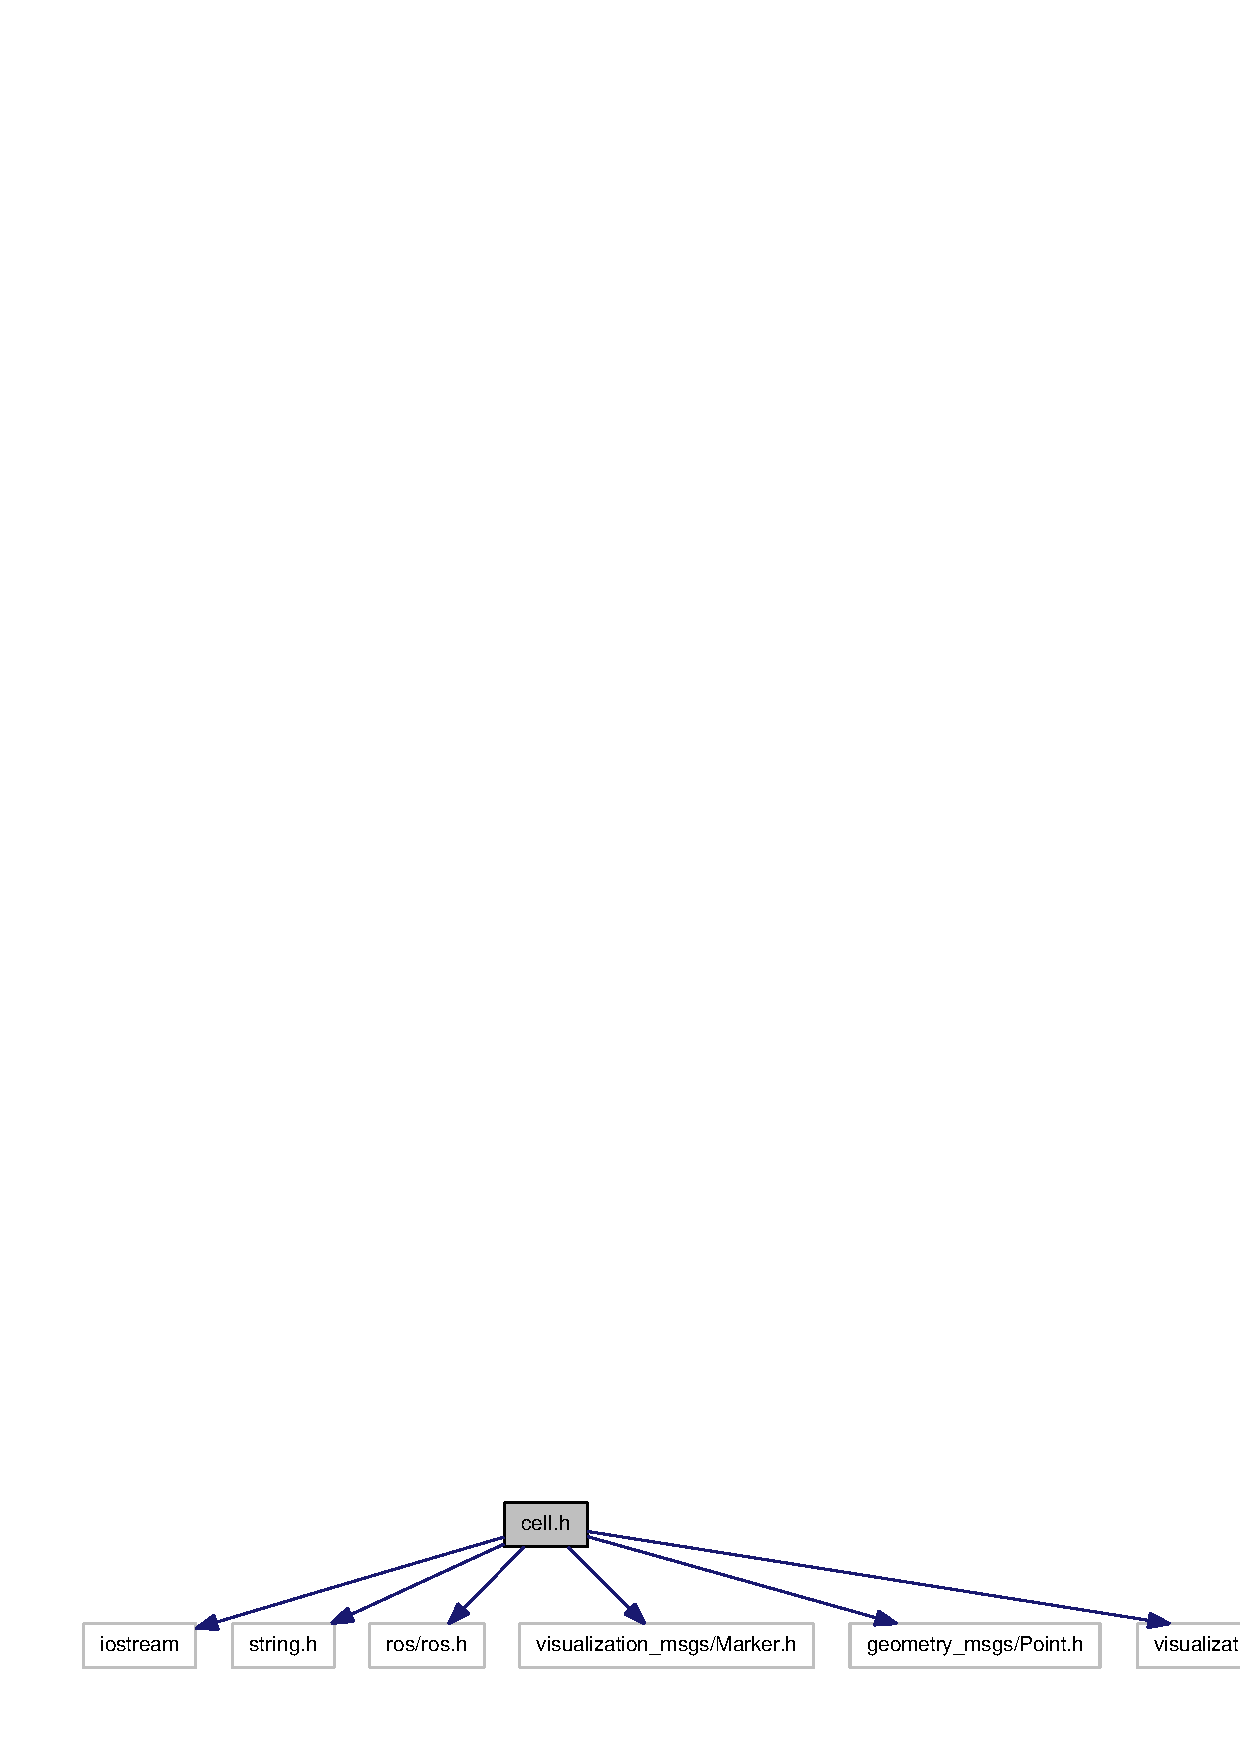
\includegraphics[width=400pt]{cell_8h__incl}
\end{center}
\end{figure}
This graph shows which files directly or indirectly include this file:
\nopagebreak
\begin{figure}[H]
\begin{center}
\leavevmode
\includegraphics[width=281pt]{cell_8h__dep__incl}
\end{center}
\end{figure}
\subsection*{Classes}
\begin{DoxyCompactItemize}
\item 
class {\bf GdmTDLAS::Cell}
\end{DoxyCompactItemize}
\subsection*{Namespaces}
\begin{DoxyCompactItemize}
\item 
namespace {\bf GdmTDLAS}
\end{DoxyCompactItemize}
\subsection*{Defines}
\begin{DoxyCompactItemize}
\item 
\#define {\bf CELL\_\-DEFAULT\_\-B}~0.0
\item 
\#define {\bf CELL\_\-DEFAULT\_\-G}~0.0
\item 
\#define {\bf CELL\_\-DEFAULT\_\-HEIGHT}~0
\item 
\#define {\bf CELL\_\-DEFAULT\_\-R}~0.0
\end{DoxyCompactItemize}


\subsection{Define Documentation}
\index{cell.h@{cell.h}!CELL\_\-DEFAULT\_\-B@{CELL\_\-DEFAULT\_\-B}}
\index{CELL\_\-DEFAULT\_\-B@{CELL\_\-DEFAULT\_\-B}!cell.h@{cell.h}}
\subsubsection[{CELL\_\-DEFAULT\_\-B}]{\setlength{\rightskip}{0pt plus 5cm}\#define CELL\_\-DEFAULT\_\-B~0.0}\label{cell_8h_aa2ced100b1b7c66c8e277c2cd6587bf6}


Definition at line 14 of file cell.h.

\index{cell.h@{cell.h}!CELL\_\-DEFAULT\_\-G@{CELL\_\-DEFAULT\_\-G}}
\index{CELL\_\-DEFAULT\_\-G@{CELL\_\-DEFAULT\_\-G}!cell.h@{cell.h}}
\subsubsection[{CELL\_\-DEFAULT\_\-G}]{\setlength{\rightskip}{0pt plus 5cm}\#define CELL\_\-DEFAULT\_\-G~0.0}\label{cell_8h_a18d783c3167cc9a555a5041a5dffbfc8}


Definition at line 13 of file cell.h.

\index{cell.h@{cell.h}!CELL\_\-DEFAULT\_\-HEIGHT@{CELL\_\-DEFAULT\_\-HEIGHT}}
\index{CELL\_\-DEFAULT\_\-HEIGHT@{CELL\_\-DEFAULT\_\-HEIGHT}!cell.h@{cell.h}}
\subsubsection[{CELL\_\-DEFAULT\_\-HEIGHT}]{\setlength{\rightskip}{0pt plus 5cm}\#define CELL\_\-DEFAULT\_\-HEIGHT~0}\label{cell_8h_add08b72f8d4cc3757bdeeeb741d4e15f}


Definition at line 15 of file cell.h.

\index{cell.h@{cell.h}!CELL\_\-DEFAULT\_\-R@{CELL\_\-DEFAULT\_\-R}}
\index{CELL\_\-DEFAULT\_\-R@{CELL\_\-DEFAULT\_\-R}!cell.h@{cell.h}}
\subsubsection[{CELL\_\-DEFAULT\_\-R}]{\setlength{\rightskip}{0pt plus 5cm}\#define CELL\_\-DEFAULT\_\-R~0.0}\label{cell_8h_a27fff0095df1dabbe4be93fe2f8103b8}


Definition at line 12 of file cell.h.


\section{Constants.hpp File Reference}
\label{Constants_8hpp}\index{Constants.hpp@{Constants.hpp}}
{\ttfamily \#include $<$qpOASES/Types.hpp$>$}\par
Include dependency graph for Constants.hpp:
\nopagebreak
\begin{figure}[H]
\begin{center}
\leavevmode
\includegraphics[width=154pt]{Constants_8hpp__incl}
\end{center}
\end{figure}
This graph shows which files directly or indirectly include this file:
\nopagebreak
\begin{figure}[H]
\begin{center}
\leavevmode
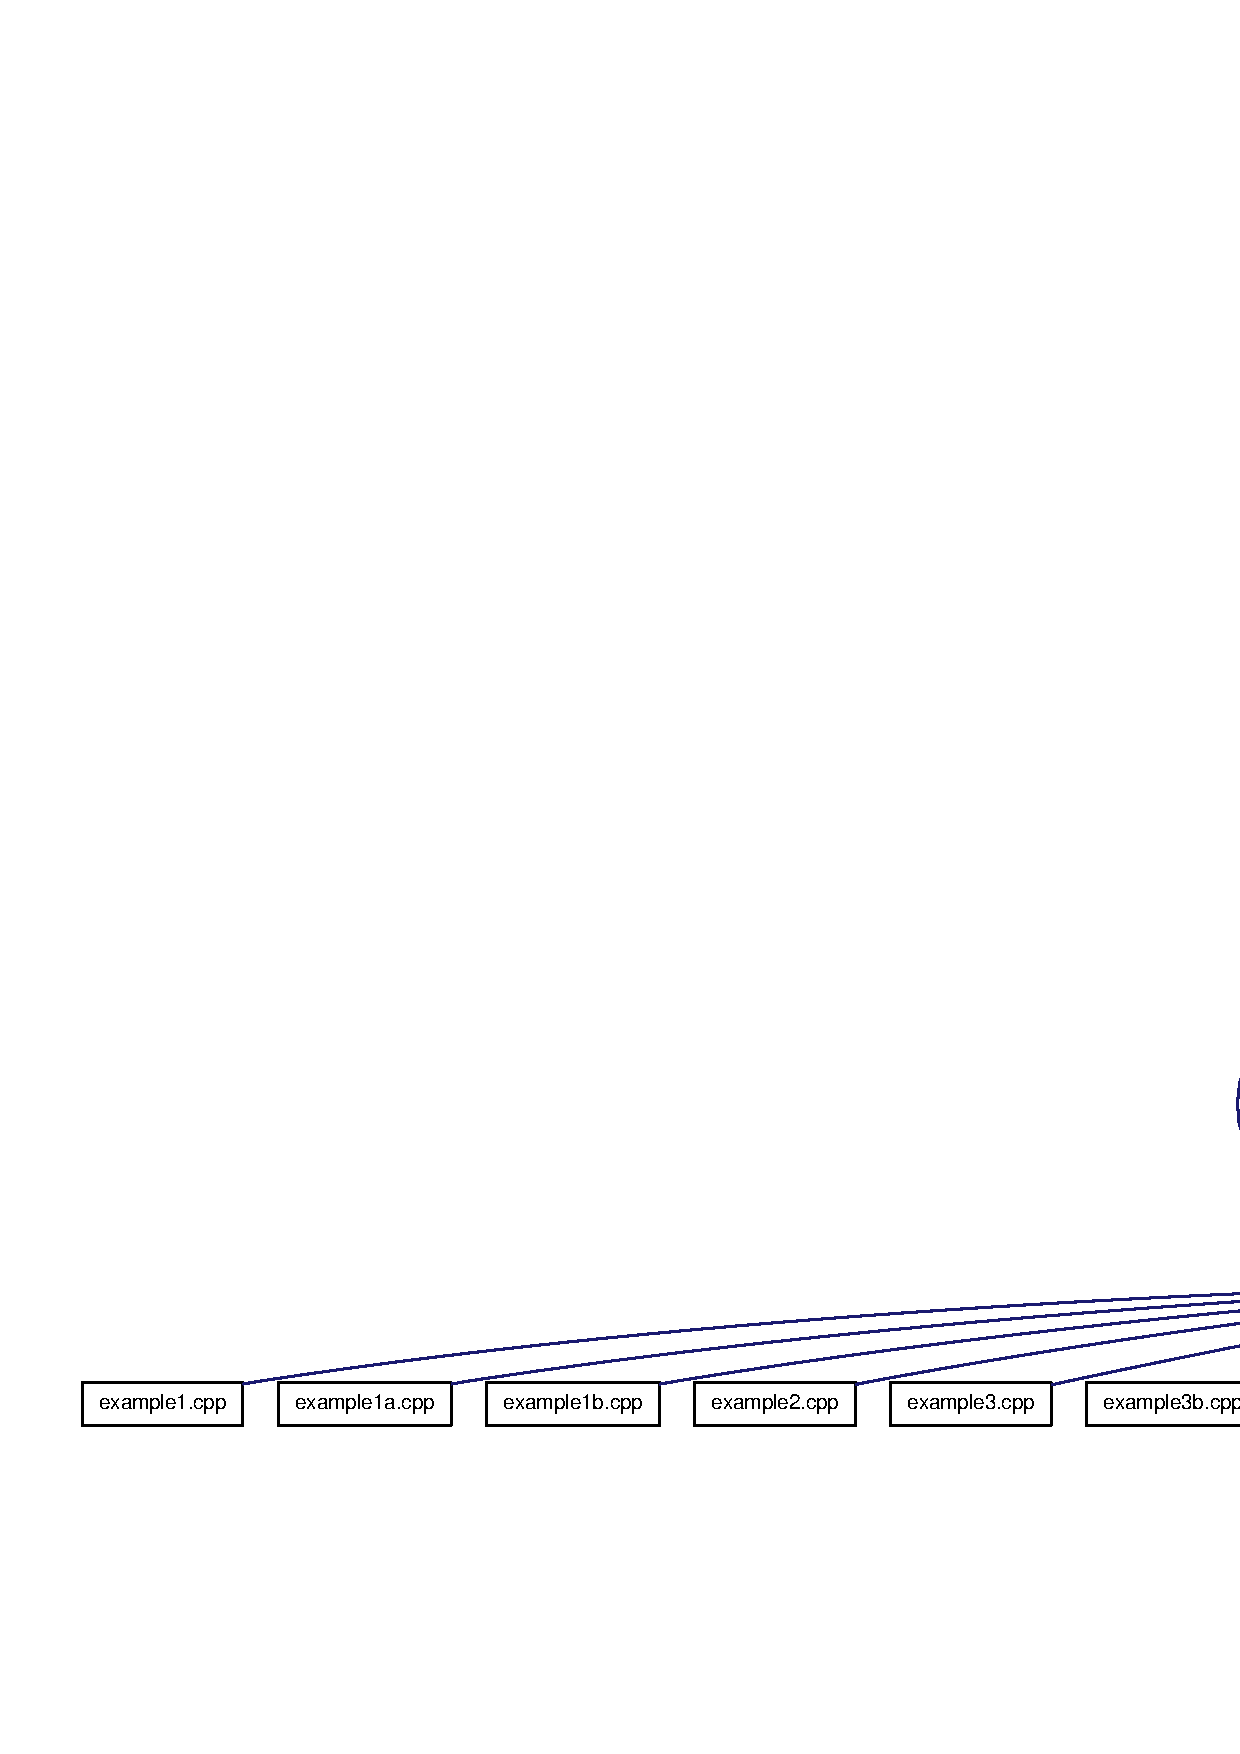
\includegraphics[width=400pt]{Constants_8hpp__dep__incl}
\end{center}
\end{figure}
\subsection*{Variables}
\begin{DoxyCompactItemize}
\item 
BEGIN\_\-NAMESPACE\_\-QPOASES const {\bf real\_\-t} {\bf EPS} = 2.221e-\/16
\item 
const {\bf real\_\-t} {\bf INFTY} = 1.0e12
\item 
const {\bf real\_\-t} {\bf ZERO} = 1.0e-\/50
\end{DoxyCompactItemize}


\subsection{Detailed Description}
\begin{DoxyAuthor}{Author}
Hans Joachim Ferreau, Andreas Potschka, Christian Kirches 
\end{DoxyAuthor}
\begin{DoxyVersion}{Version}
3.0beta 
\end{DoxyVersion}
\begin{DoxyDate}{Date}
2007-\/2012
\end{DoxyDate}
Definition of all global constants. 

Definition in file {\bf Constants.hpp}.



\subsection{Variable Documentation}
\index{Constants.hpp@{Constants.hpp}!EPS@{EPS}}
\index{EPS@{EPS}!Constants.hpp@{Constants.hpp}}
\subsubsection[{EPS}]{\setlength{\rightskip}{0pt plus 5cm}BEGIN\_\-NAMESPACE\_\-QPOASES const {\bf real\_\-t} {\bf EPS} = 2.221e-\/16}\label{Constants_8hpp_afc9ba76ddc87912abdb9b0e9029ea34e}
Numerical value of machine precision (min eps, s.t. 1+eps $>$ 1). Note: this value has to be positive! 

Definition at line 50 of file Constants.hpp.

\index{Constants.hpp@{Constants.hpp}!INFTY@{INFTY}}
\index{INFTY@{INFTY}!Constants.hpp@{Constants.hpp}}
\subsubsection[{INFTY}]{\setlength{\rightskip}{0pt plus 5cm}const {\bf real\_\-t} {\bf INFTY} = 1.0e12}\label{Constants_8hpp_a90ebbbce8b8f93a5785ca4d4d19d12a6}
Numerical value of infinity (e.g. for non-\/existing bounds). Note: this value has to be positive! 

Definition at line 61 of file Constants.hpp.

\index{Constants.hpp@{Constants.hpp}!ZERO@{ZERO}}
\index{ZERO@{ZERO}!Constants.hpp@{Constants.hpp}}
\subsubsection[{ZERO}]{\setlength{\rightskip}{0pt plus 5cm}const {\bf real\_\-t} {\bf ZERO} = 1.0e-\/50}\label{Constants_8hpp_ad819f2d51fdea4cd4ff6023e9e276e11}
Numerical value of zero (for situations in which it would be unreasonable to compare with 0.0). Note: this value has to be positive! 

Definition at line 57 of file Constants.hpp.


\section{ConstraintProduct.hpp File Reference}
\label{ConstraintProduct_8hpp}\index{ConstraintProduct.hpp@{ConstraintProduct.hpp}}
This graph shows which files directly or indirectly include this file:
\nopagebreak
\begin{figure}[H]
\begin{center}
\leavevmode
\includegraphics[width=400pt]{ConstraintProduct_8hpp__dep__incl}
\end{center}
\end{figure}
\subsection*{Classes}
\begin{DoxyCompactItemize}
\item 
class {\bf ConstraintProduct}
\begin{DoxyCompactList}\small\item\em Interface for specifying user-\/defined evaluations of constraint products. \end{DoxyCompactList}\end{DoxyCompactItemize}


\subsection{Detailed Description}
\begin{DoxyAuthor}{Author}
Hans Joachim Ferreau, Andreas Potschka, Christian Kirches 
\end{DoxyAuthor}
\begin{DoxyVersion}{Version}
3.0beta 
\end{DoxyVersion}
\begin{DoxyDate}{Date}
2009-\/2012
\end{DoxyDate}
Declaration of the \doxyref{ConstraintProduct}{p.}{classConstraintProduct} class which allows to specify a user-\/defined function for evaluating the constraint product at the current iterate to speed-\/up QP solution in case of a specially structured constraint matrix. 

Definition in file {\bf ConstraintProduct.hpp}.


\section{Constraints.cpp File Reference}
\label{Constraints_8cpp}\index{Constraints.cpp@{Constraints.cpp}}
{\ttfamily \#include $<$qpOASES/Constraints.hpp$>$}\par
Include dependency graph for Constraints.cpp:
\nopagebreak
\begin{figure}[H]
\begin{center}
\leavevmode
\includegraphics[width=400pt]{Constraints_8cpp__incl}
\end{center}
\end{figure}


\subsection{Detailed Description}
\begin{DoxyAuthor}{Author}
Hans Joachim Ferreau, Andreas Potschka, Christian Kirches 
\end{DoxyAuthor}
\begin{DoxyVersion}{Version}
3.0beta 
\end{DoxyVersion}
\begin{DoxyDate}{Date}
2007-\/2012
\end{DoxyDate}
Implementation of the \doxyref{Constraints}{p.}{classConstraints} class designed to manage working sets of constraints within a \doxyref{QProblem}{p.}{classQProblem}. 

Definition in file {\bf Constraints.cpp}.


\section{Constraints.hpp File Reference}
\label{Constraints_8hpp}\index{Constraints.hpp@{Constraints.hpp}}
{\ttfamily \#include $<$qpOASES/SubjectTo.hpp$>$}\par
{\ttfamily \#include $<$qpOASES/Constraints.ipp$>$}\par
Include dependency graph for Constraints.hpp:
\nopagebreak
\begin{figure}[H]
\begin{center}
\leavevmode
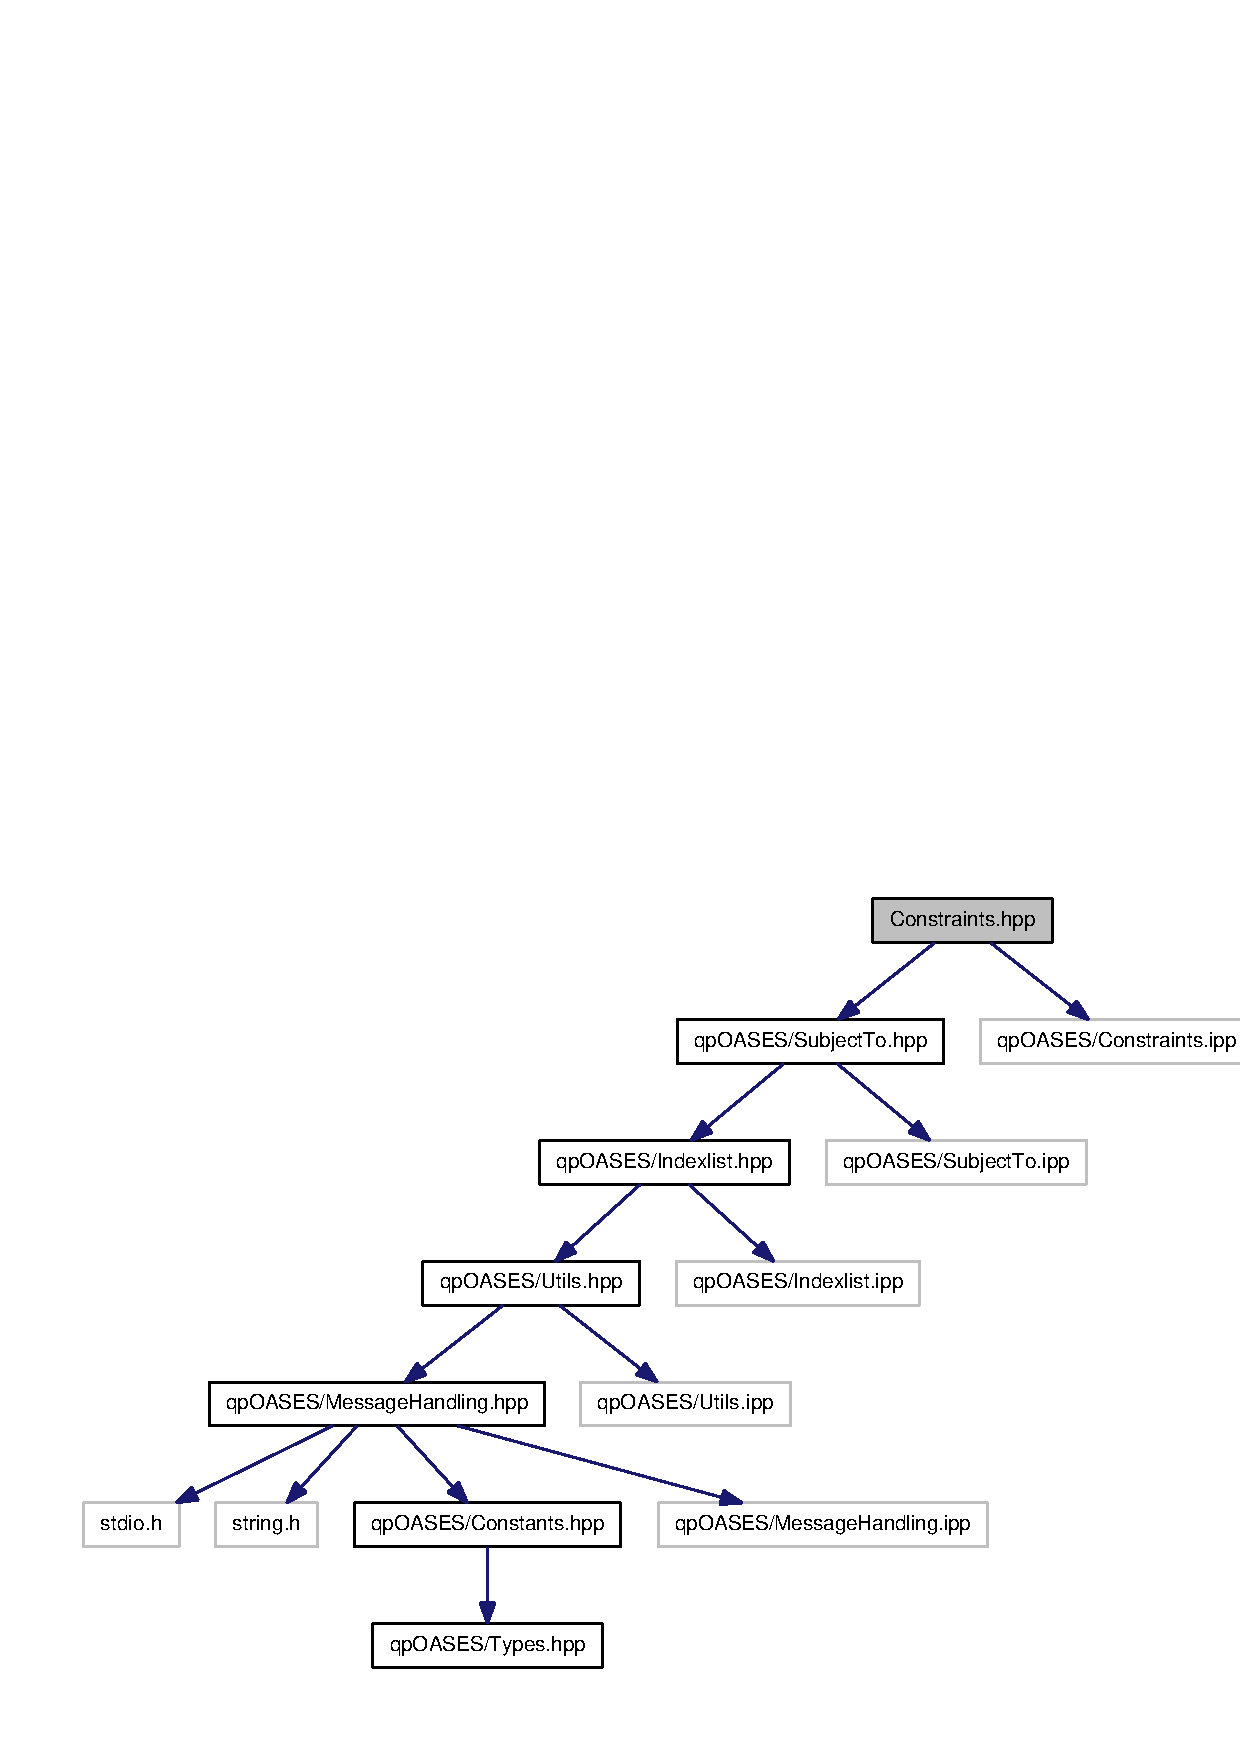
\includegraphics[width=400pt]{Constraints_8hpp__incl}
\end{center}
\end{figure}
This graph shows which files directly or indirectly include this file:
\nopagebreak
\begin{figure}[H]
\begin{center}
\leavevmode
\includegraphics[width=400pt]{Constraints_8hpp__dep__incl}
\end{center}
\end{figure}
\subsection*{Classes}
\begin{DoxyCompactItemize}
\item 
class {\bf Constraints}
\begin{DoxyCompactList}\small\item\em Manages working sets of constraints. \end{DoxyCompactList}\end{DoxyCompactItemize}


\subsection{Detailed Description}
\begin{DoxyAuthor}{Author}
Hans Joachim Ferreau, Andreas Potschka, Christian Kirches 
\end{DoxyAuthor}
\begin{DoxyVersion}{Version}
3.0beta 
\end{DoxyVersion}
\begin{DoxyDate}{Date}
2007-\/2012
\end{DoxyDate}
Declaration of the \doxyref{Constraints}{p.}{classConstraints} class designed to manage working sets of constraints within a \doxyref{QProblem}{p.}{classQProblem}. 

Definition in file {\bf Constraints.hpp}.


\section{example1.cpp File Reference}
\label{example1_8cpp}\index{example1.cpp@{example1.cpp}}
{\ttfamily \#include $<$qpOASES.hpp$>$}\par
Include dependency graph for example1.cpp:
\nopagebreak
\begin{figure}[H]
\begin{center}
\leavevmode
\includegraphics[width=400pt]{example1_8cpp__incl}
\end{center}
\end{figure}
\subsection*{Functions}
\begin{DoxyCompactItemize}
\item 
int {\bf main} ()
\end{DoxyCompactItemize}


\subsection{Detailed Description}
\begin{DoxyAuthor}{Author}
Hans Joachim Ferreau 
\end{DoxyAuthor}
\begin{DoxyVersion}{Version}
3.0beta 
\end{DoxyVersion}
\begin{DoxyDate}{Date}
2007-\/2012
\end{DoxyDate}
Very simple example for testing qpOASES (using \doxyref{QProblem}{p.}{classQProblem} class). 

Definition in file {\bf example1.cpp}.



\subsection{Function Documentation}
\index{example1.cpp@{example1.cpp}!main@{main}}
\index{main@{main}!example1.cpp@{example1.cpp}}
\subsubsection[{main}]{\setlength{\rightskip}{0pt plus 5cm}int main (
\begin{DoxyParamCaption}
{}
\end{DoxyParamCaption}
)}\label{example1_8cpp_ae66f6b31b5ad750f1fe042a706a4e3d4}
Example for qpOASES main function using the \doxyref{QProblem}{p.}{classQProblem} class. 

Definition at line 40 of file example1.cpp.


\section{example1a.cpp File Reference}
\label{example1a_8cpp}\index{example1a.cpp@{example1a.cpp}}
{\ttfamily \#include $<$qpOASES.hpp$>$}\par
Include dependency graph for example1a.cpp:
\nopagebreak
\begin{figure}[H]
\begin{center}
\leavevmode
\includegraphics[width=400pt]{example1a_8cpp__incl}
\end{center}
\end{figure}
\subsection*{Functions}
\begin{DoxyCompactItemize}
\item 
int {\bf main} ()
\end{DoxyCompactItemize}


\subsection{Detailed Description}
\begin{DoxyAuthor}{Author}
Hans Joachim Ferreau 
\end{DoxyAuthor}
\begin{DoxyVersion}{Version}
3.0beta 
\end{DoxyVersion}
\begin{DoxyDate}{Date}
2007-\/2012
\end{DoxyDate}
Very simple example for testing qpOASES using the \doxyref{SQProblem}{p.}{classSQProblem} class. 

Definition in file {\bf example1a.cpp}.



\subsection{Function Documentation}
\index{example1a.cpp@{example1a.cpp}!main@{main}}
\index{main@{main}!example1a.cpp@{example1a.cpp}}
\subsubsection[{main}]{\setlength{\rightskip}{0pt plus 5cm}int main (
\begin{DoxyParamCaption}
{}
\end{DoxyParamCaption}
)}\label{example1a_8cpp_ae66f6b31b5ad750f1fe042a706a4e3d4}
Example for qpOASES main function using the \doxyref{SQProblem}{p.}{classSQProblem} class. 

Definition at line 40 of file example1a.cpp.


\section{example1b.cpp File Reference}
\label{example1b_8cpp}\index{example1b.cpp@{example1b.cpp}}
{\ttfamily \#include $<$qpOASES.hpp$>$}\par
Include dependency graph for example1b.cpp:
\nopagebreak
\begin{figure}[H]
\begin{center}
\leavevmode
\includegraphics[width=400pt]{example1b_8cpp__incl}
\end{center}
\end{figure}
\subsection*{Functions}
\begin{DoxyCompactItemize}
\item 
int {\bf main} ()
\end{DoxyCompactItemize}


\subsection{Detailed Description}
\begin{DoxyAuthor}{Author}
Hans Joachim Ferreau 
\end{DoxyAuthor}
\begin{DoxyVersion}{Version}
3.0beta 
\end{DoxyVersion}
\begin{DoxyDate}{Date}
2007-\/2012
\end{DoxyDate}
Very simple example for testing qpOASES using the \doxyref{QProblemB}{p.}{classQProblemB} class. 

Definition in file {\bf example1b.cpp}.



\subsection{Function Documentation}
\index{example1b.cpp@{example1b.cpp}!main@{main}}
\index{main@{main}!example1b.cpp@{example1b.cpp}}
\subsubsection[{main}]{\setlength{\rightskip}{0pt plus 5cm}int main (
\begin{DoxyParamCaption}
{}
\end{DoxyParamCaption}
)}\label{example1b_8cpp_ae66f6b31b5ad750f1fe042a706a4e3d4}
Example for qpOASES main function using the \doxyref{QProblemB}{p.}{classQProblemB} class. 

Definition at line 39 of file example1b.cpp.


\section{example2.cpp File Reference}
\label{example2_8cpp}\index{example2.cpp@{example2.cpp}}
{\ttfamily \#include $<$qpOASES.hpp$>$}\par
Include dependency graph for example2.cpp:
\nopagebreak
\begin{figure}[H]
\begin{center}
\leavevmode
\includegraphics[width=400pt]{example2_8cpp__incl}
\end{center}
\end{figure}
\subsection*{Functions}
\begin{DoxyCompactItemize}
\item 
int {\bf main} ()
\end{DoxyCompactItemize}


\subsection{Detailed Description}
\begin{DoxyAuthor}{Author}
Boris Houska, Hans Joachim Ferreau 
\end{DoxyAuthor}
\begin{DoxyVersion}{Version}
3.0beta 
\end{DoxyVersion}
\begin{DoxyDate}{Date}
2008-\/2009
\end{DoxyDate}
Very simple example for testing qpOASES in combination with the \doxyref{SolutionAnalysis}{p.}{classSolutionAnalysis} class. 

Definition in file {\bf example2.cpp}.



\subsection{Function Documentation}
\index{example2.cpp@{example2.cpp}!main@{main}}
\index{main@{main}!example2.cpp@{example2.cpp}}
\subsubsection[{main}]{\setlength{\rightskip}{0pt plus 5cm}int main (
\begin{DoxyParamCaption}
{}
\end{DoxyParamCaption}
)}\label{example2_8cpp_ae66f6b31b5ad750f1fe042a706a4e3d4}
Example for qpOASES main function using the \doxyref{SolutionAnalysis}{p.}{classSolutionAnalysis} class. 

Definition at line 41 of file example2.cpp.


\input{example3_8cpp}
\section{example3b.cpp File Reference}
\label{example3b_8cpp}\index{example3b.cpp@{example3b.cpp}}
{\ttfamily \#include $<$qpOASES.hpp$>$}\par
Include dependency graph for example3b.cpp:
\nopagebreak
\begin{figure}[H]
\begin{center}
\leavevmode
\includegraphics[width=400pt]{example3b_8cpp__incl}
\end{center}
\end{figure}
\subsection*{Functions}
\begin{DoxyCompactItemize}
\item 
int {\bf main} ()
\end{DoxyCompactItemize}


\subsection{Detailed Description}
\begin{DoxyAuthor}{Author}
Hans Joachim Ferreau 
\end{DoxyAuthor}
\begin{DoxyVersion}{Version}
3.0beta 
\end{DoxyVersion}
\begin{DoxyDate}{Date}
2008-\/2009
\end{DoxyDate}
Example demonstrating usage of qpOASES for solving a QP sequence of the Online QP Benchmark Collection. In order to run it, you have to download \char`\"{}Example 02\char`\"{} from {\tt http://homes.esat.kuleuven.be/$\sim$optec/software/onlineQP/} and store it into the directory EXAMPLES/chain80/. 

Definition in file {\bf example3b.cpp}.



\subsection{Function Documentation}
\index{example3b.cpp@{example3b.cpp}!main@{main}}
\index{main@{main}!example3b.cpp@{example3b.cpp}}
\subsubsection[{main}]{\setlength{\rightskip}{0pt plus 5cm}int main (
\begin{DoxyParamCaption}
{}
\end{DoxyParamCaption}
)}\label{example3b_8cpp_ae66f6b31b5ad750f1fe042a706a4e3d4}
Example for qpOASES main function using the OQP interface. 

Definition at line 43 of file example3b.cpp.


\section{example4.cpp File Reference}
\label{example4_8cpp}\index{example4.cpp@{example4.cpp}}
{\ttfamily \#include $<$stdlib.h$>$}\par
{\ttfamily \#include $<$qpOASES.hpp$>$}\par
{\ttfamily \#include \char`\"{}example4CP.cpp\char`\"{}}\par
Include dependency graph for example4.cpp:
\nopagebreak
\begin{figure}[H]
\begin{center}
\leavevmode
\includegraphics[width=400pt]{example4_8cpp__incl}
\end{center}
\end{figure}
\subsection*{Functions}
\begin{DoxyCompactItemize}
\item 
int {\bf main} ()
\end{DoxyCompactItemize}


\subsection{Detailed Description}
\begin{DoxyAuthor}{Author}
Hans Joachim Ferreau 
\end{DoxyAuthor}
\begin{DoxyVersion}{Version}
3.0beta 
\end{DoxyVersion}
\begin{DoxyDate}{Date}
2009
\end{DoxyDate}
Very simple example for testing qpOASES (using the possibility to specify user-\/defined constraint product function). 

Definition in file {\bf example4.cpp}.



\subsection{Function Documentation}
\index{example4.cpp@{example4.cpp}!main@{main}}
\index{main@{main}!example4.cpp@{example4.cpp}}
\subsubsection[{main}]{\setlength{\rightskip}{0pt plus 5cm}int main (
\begin{DoxyParamCaption}
{}
\end{DoxyParamCaption}
)}\label{example4_8cpp_ae66f6b31b5ad750f1fe042a706a4e3d4}
Example for qpOASES main function using the possibility to specify user-\/defined constraint product function. 

Definition at line 45 of file example4.cpp.


\section{example4CP.cpp File Reference}
\label{example4CP_8cpp}\index{example4CP.cpp@{example4CP.cpp}}
This graph shows which files directly or indirectly include this file:
\nopagebreak
\begin{figure}[H]
\begin{center}
\leavevmode
\includegraphics[width=214pt]{example4CP_8cpp__dep__incl}
\end{center}
\end{figure}
\subsection*{Classes}
\begin{DoxyCompactItemize}
\item 
class {\bf MyConstraintProduct}
\begin{DoxyCompactList}\small\item\em Example illustrating the use of the {\itshape \doxyref{ConstraintProduct}{p.}{classConstraintProduct}\/} class. \end{DoxyCompactList}\end{DoxyCompactItemize}


\subsection{Detailed Description}
\begin{DoxyAuthor}{Author}
Hans Joachim Ferreau 
\end{DoxyAuthor}
\begin{DoxyVersion}{Version}
3.0beta 
\end{DoxyVersion}
\begin{DoxyDate}{Date}
2009
\end{DoxyDate}
Sample implementation of the \doxyref{ConstraintProduct}{p.}{classConstraintProduct} class tailored for Example4. 

Definition in file {\bf example4CP.cpp}.


\section{example5.cpp File Reference}
\label{example5_8cpp}\index{example5.cpp@{example5.cpp}}
{\ttfamily \#include $<$stdlib.h$>$}\par
{\ttfamily \#include $<$qpOASES.hpp$>$}\par
{\ttfamily \#include \char`\"{}example4CP.cpp\char`\"{}}\par
Include dependency graph for example5.cpp:
\nopagebreak
\begin{figure}[H]
\begin{center}
\leavevmode
\includegraphics[width=400pt]{example5_8cpp__incl}
\end{center}
\end{figure}
\subsection*{Functions}
\begin{DoxyCompactItemize}
\item 
int {\bf main} ()
\end{DoxyCompactItemize}


\subsection{Detailed Description}
\begin{DoxyAuthor}{Author}
Andreas Potschka, Christian Kirches 
\end{DoxyAuthor}
\begin{DoxyVersion}{Version}
3.0beta 
\end{DoxyVersion}
\begin{DoxyDate}{Date}
2011
\end{DoxyDate}
Very simple example for testing qpOASES (using the possibility to compute the local linear feedback law) 

Definition in file {\bf example5.cpp}.



\subsection{Function Documentation}
\index{example5.cpp@{example5.cpp}!main@{main}}
\index{main@{main}!example5.cpp@{example5.cpp}}
\subsubsection[{main}]{\setlength{\rightskip}{0pt plus 5cm}int main (
\begin{DoxyParamCaption}
{}
\end{DoxyParamCaption}
)}\label{example5_8cpp_ae66f6b31b5ad750f1fe042a706a4e3d4}
Example for qpOASES main function using the possibility to specify user-\/defined constraint product function. 

Definition at line 45 of file example5.cpp.


\section{example6.cpp File Reference}
\label{example6_8cpp}\index{example6.cpp@{example6.cpp}}
{\ttfamily \#include $<$qpOASES.hpp$>$}\par
Include dependency graph for example6.cpp:
\nopagebreak
\begin{figure}[H]
\begin{center}
\leavevmode
\includegraphics[width=400pt]{example6_8cpp__incl}
\end{center}
\end{figure}
\subsection*{Functions}
\begin{DoxyCompactItemize}
\item 
int {\bf main} ()
\end{DoxyCompactItemize}


\subsection{Detailed Description}
\begin{DoxyAuthor}{Author}
Hans Joachim Ferreau 
\end{DoxyAuthor}
\begin{DoxyVersion}{Version}
3.0beta 
\end{DoxyVersion}
\begin{DoxyDate}{Date}
2007-\/2012
\end{DoxyDate}
Very simple example for testing qpOASES (using \doxyref{QProblem}{p.}{classQProblem} class). 

Definition in file {\bf example6.cpp}.



\subsection{Function Documentation}
\index{example6.cpp@{example6.cpp}!main@{main}}
\index{main@{main}!example6.cpp@{example6.cpp}}
\subsubsection[{main}]{\setlength{\rightskip}{0pt plus 5cm}int main (
\begin{DoxyParamCaption}
{}
\end{DoxyParamCaption}
)}\label{example6_8cpp_ae66f6b31b5ad750f1fe042a706a4e3d4}
Example for qpOASES main function using the \doxyref{QProblem}{p.}{classQProblem} class. 

Definition at line 40 of file example6.cpp.


\section{exampleLP.cpp File Reference}
\label{exampleLP_8cpp}\index{exampleLP.cpp@{exampleLP.cpp}}
{\ttfamily \#include $<$qpOASES.hpp$>$}\par
Include dependency graph for exampleLP.cpp:
\nopagebreak
\begin{figure}[H]
\begin{center}
\leavevmode
\includegraphics[width=400pt]{exampleLP_8cpp__incl}
\end{center}
\end{figure}
\subsection*{Functions}
\begin{DoxyCompactItemize}
\item 
int {\bf main} ()
\end{DoxyCompactItemize}


\subsection{Detailed Description}
\begin{DoxyAuthor}{Author}
Hans Joachim Ferreau 
\end{DoxyAuthor}
\begin{DoxyVersion}{Version}
3.0beta 
\end{DoxyVersion}
\begin{DoxyDate}{Date}
2008-\/2009
\end{DoxyDate}
Very simple example for solving a LP sequence using qpOASES. 

Definition in file {\bf exampleLP.cpp}.



\subsection{Function Documentation}
\index{exampleLP.cpp@{exampleLP.cpp}!main@{main}}
\index{main@{main}!exampleLP.cpp@{exampleLP.cpp}}
\subsubsection[{main}]{\setlength{\rightskip}{0pt plus 5cm}int main (
\begin{DoxyParamCaption}
{}
\end{DoxyParamCaption}
)}\label{exampleLP_8cpp_ae66f6b31b5ad750f1fe042a706a4e3d4}
Example for qpOASES main function solving LPs. 

Definition at line 40 of file exampleLP.cpp.


\section{Flipper.cpp File Reference}
\label{Flipper_8cpp}\index{Flipper.cpp@{Flipper.cpp}}
{\ttfamily \#include $<$qpOASES/Flipper.hpp$>$}\par
Include dependency graph for Flipper.cpp:
\nopagebreak
\begin{figure}[H]
\begin{center}
\leavevmode
\includegraphics[width=400pt]{Flipper_8cpp__incl}
\end{center}
\end{figure}


\subsection{Detailed Description}
\begin{DoxyAuthor}{Author}
Hans Joachim Ferreau, Andreas Potschka, Christian Kirches 
\end{DoxyAuthor}
\begin{DoxyVersion}{Version}
3.0beta 
\end{DoxyVersion}
\begin{DoxyDate}{Date}
2007-\/2012
\end{DoxyDate}
Implementation of the \doxyref{Flipper}{p.}{classFlipper} class designed to manage working sets of constraints and bounds within a \doxyref{QProblem}{p.}{classQProblem}. 

Definition in file {\bf Flipper.cpp}.


\section{Flipper.hpp File Reference}
\label{Flipper_8hpp}\index{Flipper.hpp@{Flipper.hpp}}
{\ttfamily \#include $<$qpOASES/Bounds.hpp$>$}\par
{\ttfamily \#include $<$qpOASES/Constraints.hpp$>$}\par
Include dependency graph for Flipper.hpp:
\nopagebreak
\begin{figure}[H]
\begin{center}
\leavevmode
\includegraphics[width=400pt]{Flipper_8hpp__incl}
\end{center}
\end{figure}
This graph shows which files directly or indirectly include this file:
\nopagebreak
\begin{figure}[H]
\begin{center}
\leavevmode
\includegraphics[width=400pt]{Flipper_8hpp__dep__incl}
\end{center}
\end{figure}
\subsection*{Classes}
\begin{DoxyCompactItemize}
\item 
class {\bf Flipper}
\begin{DoxyCompactList}\small\item\em Auxiliary class for storing a copy of the current matrix factorisations. \end{DoxyCompactList}\end{DoxyCompactItemize}


\subsection{Detailed Description}
\begin{DoxyAuthor}{Author}
Hans Joachim Ferreau, Andreas Potschka, Christian Kirches 
\end{DoxyAuthor}
\begin{DoxyVersion}{Version}
3.0beta 
\end{DoxyVersion}
\begin{DoxyDate}{Date}
2007-\/2012
\end{DoxyDate}
Declaration of the \doxyref{Options}{p.}{classOptions} class designed to manage user-\/specified options for solving a \doxyref{QProblem}{p.}{classQProblem}. 

Definition in file {\bf Flipper.hpp}.


\section{gdm\_\-tdlas.cpp File Reference}
\label{gdm__tdlas_8cpp}\index{gdm\_\-tdlas.cpp@{gdm\_\-tdlas.cpp}}
{\ttfamily \#include \char`\"{}gdm\_\-tdlas.h\char`\"{}}\par
{\ttfamily \#include \char`\"{}std\_\-msgs/Float32.h\char`\"{}}\par
Include dependency graph for gdm\_\-tdlas.cpp:
\nopagebreak
\begin{figure}[H]
\begin{center}
\leavevmode
\includegraphics[width=400pt]{gdm__tdlas_8cpp__incl}
\end{center}
\end{figure}
\subsection*{Functions}
\begin{DoxyCompactItemize}
\item 
int {\bf main} (int argc, char $\ast$$\ast$argv)
\item 
void {\bf printSparseMatrixInfo} (vector$<$ {\bf sparse\_\-int\_\-t} $>$ $\ast${\bf H\_\-jc}, vector$<$ {\bf sparse\_\-int\_\-t} $>$ $\ast${\bf H\_\-ir}, vector$<$ {\bf real\_\-t} $>$ $\ast${\bf H\_\-val})
\item 
void {\bf rmldInCallback} (const {\bf localized\_\-RMLD::rmld\_\-msg::ConstPtr} \&msg\_\-in)
\item 
void {\bf updateGradient} ({\bf real\_\-t} $\ast${\bf g}, std::vector$<$ int $>$ $\ast$idx, std::vector$<$ float $>$ $\ast$val, float ppmm)
\item 
void {\bf updateHessian} (vector$<$ {\bf sparse\_\-int\_\-t} $>$ $\ast${\bf H\_\-jc}, vector$<$ {\bf sparse\_\-int\_\-t} $>$ $\ast${\bf H\_\-ir}, vector$<$ {\bf real\_\-t} $>$ $\ast${\bf H\_\-val}, std::vector$<$ int $>$ $\ast$idx, std::vector$<$ float $>$ $\ast$val)
\end{DoxyCompactItemize}


\subsection{Function Documentation}
\index{gdm\_\-tdlas.cpp@{gdm\_\-tdlas.cpp}!main@{main}}
\index{main@{main}!gdm_tdlas.cpp@{gdm\_\-tdlas.cpp}}
\subsubsection[{main}]{\setlength{\rightskip}{0pt plus 5cm}int main (
\begin{DoxyParamCaption}
\item[{int}]{argc, }
\item[{char $\ast$$\ast$}]{argv}
\end{DoxyParamCaption}
)}\label{gdm__tdlas_8cpp_a3c04138a5bfe5d72780bb7e82a18e627}


Definition at line 122 of file gdm\_\-tdlas.cpp.

\index{gdm\_\-tdlas.cpp@{gdm\_\-tdlas.cpp}!printSparseMatrixInfo@{printSparseMatrixInfo}}
\index{printSparseMatrixInfo@{printSparseMatrixInfo}!gdm_tdlas.cpp@{gdm\_\-tdlas.cpp}}
\subsubsection[{printSparseMatrixInfo}]{\setlength{\rightskip}{0pt plus 5cm}void printSparseMatrixInfo (
\begin{DoxyParamCaption}
\item[{vector$<$ {\bf sparse\_\-int\_\-t} $>$ $\ast$}]{H\_\-jc, }
\item[{vector$<$ {\bf sparse\_\-int\_\-t} $>$ $\ast$}]{H\_\-ir, }
\item[{vector$<$ {\bf real\_\-t} $>$ $\ast$}]{H\_\-val}
\end{DoxyParamCaption}
)}\label{gdm__tdlas_8cpp_a770fbb72148815e193cb914c3b90672e}


Definition at line 62 of file gdm\_\-tdlas.cpp.

\index{gdm\_\-tdlas.cpp@{gdm\_\-tdlas.cpp}!rmldInCallback@{rmldInCallback}}
\index{rmldInCallback@{rmldInCallback}!gdm_tdlas.cpp@{gdm\_\-tdlas.cpp}}
\subsubsection[{rmldInCallback}]{\setlength{\rightskip}{0pt plus 5cm}void rmldInCallback (
\begin{DoxyParamCaption}
\item[{const {\bf localized\_\-RMLD::rmld\_\-msg::ConstPtr} \&}]{msg\_\-in}
\end{DoxyParamCaption}
)}\label{gdm__tdlas_8cpp_a9292cdb1fe5d1204ecdbebe741c53c0a}


Definition at line 42 of file gdm\_\-tdlas.cpp.

\index{gdm\_\-tdlas.cpp@{gdm\_\-tdlas.cpp}!updateGradient@{updateGradient}}
\index{updateGradient@{updateGradient}!gdm_tdlas.cpp@{gdm\_\-tdlas.cpp}}
\subsubsection[{updateGradient}]{\setlength{\rightskip}{0pt plus 5cm}void updateGradient (
\begin{DoxyParamCaption}
\item[{{\bf real\_\-t} $\ast$}]{g, }
\item[{std::vector$<$ int $>$ $\ast$}]{idx, }
\item[{std::vector$<$ float $>$ $\ast$}]{val, }
\item[{float}]{ppmm}
\end{DoxyParamCaption}
)}\label{gdm__tdlas_8cpp_a2cce26a45fa8cc7c05809eda69e50caf}


Definition at line 56 of file gdm\_\-tdlas.cpp.

\index{gdm\_\-tdlas.cpp@{gdm\_\-tdlas.cpp}!updateHessian@{updateHessian}}
\index{updateHessian@{updateHessian}!gdm_tdlas.cpp@{gdm\_\-tdlas.cpp}}
\subsubsection[{updateHessian}]{\setlength{\rightskip}{0pt plus 5cm}void updateHessian (
\begin{DoxyParamCaption}
\item[{vector$<$ {\bf sparse\_\-int\_\-t} $>$ $\ast$}]{H\_\-jc, }
\item[{vector$<$ {\bf sparse\_\-int\_\-t} $>$ $\ast$}]{H\_\-ir, }
\item[{vector$<$ {\bf real\_\-t} $>$ $\ast$}]{H\_\-val, }
\item[{std::vector$<$ int $>$ $\ast$}]{idx, }
\item[{std::vector$<$ float $>$ $\ast$}]{val}
\end{DoxyParamCaption}
)}\label{gdm__tdlas_8cpp_ab675358ab25a01aba70d16afe129fcfc}


Definition at line 75 of file gdm\_\-tdlas.cpp.


\section{gdm\_\-tdlas.h File Reference}
\label{gdm__tdlas_8h}\index{gdm\_\-tdlas.h@{gdm\_\-tdlas.h}}
{\ttfamily \#include \char`\"{}rmld\_\-msg.h\char`\"{}}\par
{\ttfamily \#include \char`\"{}ros/ros.h\char`\"{}}\par
{\ttfamily \#include \char`\"{}std\_\-msgs/String.h\char`\"{}}\par
{\ttfamily \#include \char`\"{}map.h\char`\"{}}\par
{\ttfamily \#include $<$stdio.h$>$}\par
{\ttfamily \#include $<$string.h$>$}\par
{\ttfamily \#include $<$geometry\_\-msgs/Point.h$>$}\par
{\ttfamily \#include $<$boost/thread/mutex.hpp$>$}\par
{\ttfamily \#include $<$boost/math/constants/constants.hpp$>$}\par
{\ttfamily \#include $<$qpOASES.hpp$>$}\par
Include dependency graph for gdm\_\-tdlas.h:
\nopagebreak
\begin{figure}[H]
\begin{center}
\leavevmode
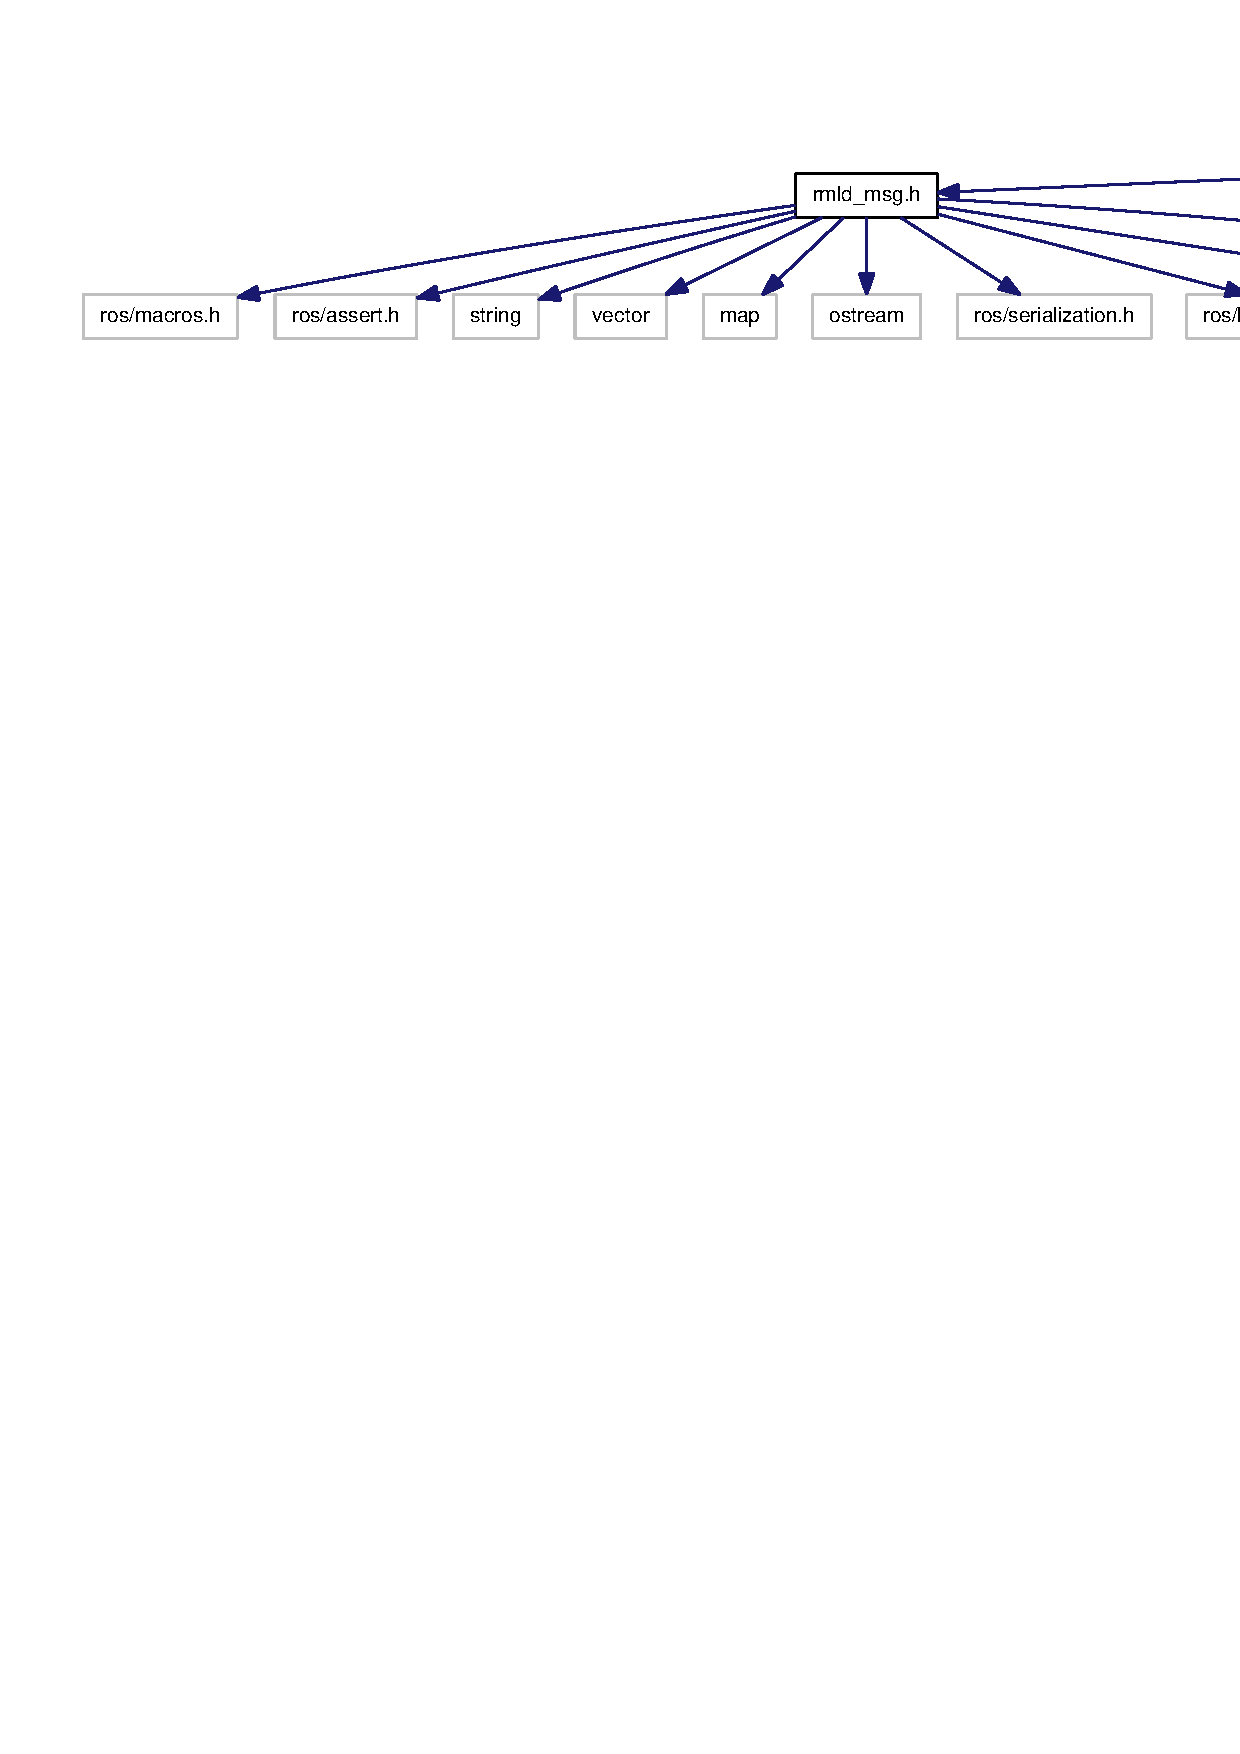
\includegraphics[width=400pt]{gdm__tdlas_8h__incl}
\end{center}
\end{figure}
This graph shows which files directly or indirectly include this file:
\nopagebreak
\begin{figure}[H]
\begin{center}
\leavevmode
\includegraphics[width=124pt]{gdm__tdlas_8h__dep__incl}
\end{center}
\end{figure}
\subsection*{Defines}
\begin{DoxyCompactItemize}
\item 
\#define {\bf LOOP\_\-RATE\_\-HZ}~50
\item 
\#define {\bf NODE\_\-NAME}~\char`\"{}gdm\_\-tdlas\char`\"{}
\end{DoxyCompactItemize}
\subsection*{Variables}
\begin{DoxyCompactItemize}
\item 
double {\bf CELL\_\-SIZE} = 1
\item 
std::string {\bf FIXED\_\-FRAME} = \char`\"{}/map\char`\"{}
\item 
{\bf GdmTDLAS::GasMap} $\ast$ {\bf gas\_\-map}
\item 
geometry\_\-msgs::Point {\bf lastPoint\_\-End}
\item 
geometry\_\-msgs::Point {\bf lastPoint\_\-Origin}
\item 
double {\bf MAX\_\-CONC} = 100
\item 
double {\bf MAX\_\-X} = 6.00
\item 
double {\bf MAX\_\-Y} = 15.00
\item 
float {\bf measurementPPMM}
\item 
double {\bf MIN\_\-X} = -\/5.30
\item 
double {\bf MIN\_\-Y} = -\/3.09
\item 
boost::mutex {\bf mutex\_\-rmld}
\item 
bool {\bf new\_\-data\_\-arrived}
\item 
std::string {\bf RMLD\_\-TOPIC} = \char`\"{}localized\_\-RMLD/rmld\_\-data\char`\"{}
\end{DoxyCompactItemize}


\subsection{Define Documentation}
\index{gdm\_\-tdlas.h@{gdm\_\-tdlas.h}!LOOP\_\-RATE\_\-HZ@{LOOP\_\-RATE\_\-HZ}}
\index{LOOP\_\-RATE\_\-HZ@{LOOP\_\-RATE\_\-HZ}!gdm_tdlas.h@{gdm\_\-tdlas.h}}
\subsubsection[{LOOP\_\-RATE\_\-HZ}]{\setlength{\rightskip}{0pt plus 5cm}\#define LOOP\_\-RATE\_\-HZ~50}\label{gdm__tdlas_8h_acd97b33c4ed6a53a3c744ea2f76bd378}


Definition at line 51 of file gdm\_\-tdlas.h.

\index{gdm\_\-tdlas.h@{gdm\_\-tdlas.h}!NODE\_\-NAME@{NODE\_\-NAME}}
\index{NODE\_\-NAME@{NODE\_\-NAME}!gdm_tdlas.h@{gdm\_\-tdlas.h}}
\subsubsection[{NODE\_\-NAME}]{\setlength{\rightskip}{0pt plus 5cm}\#define NODE\_\-NAME~\char`\"{}gdm\_\-tdlas\char`\"{}}\label{gdm__tdlas_8h_a8cc8d559acdd2f74085b20977182d5b7}


Definition at line 52 of file gdm\_\-tdlas.h.



\subsection{Variable Documentation}
\index{gdm\_\-tdlas.h@{gdm\_\-tdlas.h}!CELL\_\-SIZE@{CELL\_\-SIZE}}
\index{CELL\_\-SIZE@{CELL\_\-SIZE}!gdm_tdlas.h@{gdm\_\-tdlas.h}}
\subsubsection[{CELL\_\-SIZE}]{\setlength{\rightskip}{0pt plus 5cm}double {\bf CELL\_\-SIZE} = 1}\label{gdm__tdlas_8h_a4cf9ff51a66312cba25005de9de38c30}


Definition at line 60 of file gdm\_\-tdlas.h.

\index{gdm\_\-tdlas.h@{gdm\_\-tdlas.h}!FIXED\_\-FRAME@{FIXED\_\-FRAME}}
\index{FIXED\_\-FRAME@{FIXED\_\-FRAME}!gdm_tdlas.h@{gdm\_\-tdlas.h}}
\subsubsection[{FIXED\_\-FRAME}]{\setlength{\rightskip}{0pt plus 5cm}std::string {\bf FIXED\_\-FRAME} = \char`\"{}/map\char`\"{}}\label{gdm__tdlas_8h_ae723813911dffa4fe96261e3bc59c131}


Definition at line 64 of file gdm\_\-tdlas.h.

\index{gdm\_\-tdlas.h@{gdm\_\-tdlas.h}!gas\_\-map@{gas\_\-map}}
\index{gas\_\-map@{gas\_\-map}!gdm_tdlas.h@{gdm\_\-tdlas.h}}
\subsubsection[{gas\_\-map}]{\setlength{\rightskip}{0pt plus 5cm}{\bf GdmTDLAS::GasMap}$\ast$ {\bf gas\_\-map}}\label{gdm__tdlas_8h_ade0f976bd45ebb046e717c19f8361b8a}


Definition at line 82 of file gdm\_\-tdlas.h.

\index{gdm\_\-tdlas.h@{gdm\_\-tdlas.h}!lastPoint\_\-End@{lastPoint\_\-End}}
\index{lastPoint\_\-End@{lastPoint\_\-End}!gdm_tdlas.h@{gdm\_\-tdlas.h}}
\subsubsection[{lastPoint\_\-End}]{\setlength{\rightskip}{0pt plus 5cm}geometry\_\-msgs::Point {\bf lastPoint\_\-End}}\label{gdm__tdlas_8h_aa9e3139dbb4679af2b6dfab4559ac517}


Definition at line 78 of file gdm\_\-tdlas.h.

\index{gdm\_\-tdlas.h@{gdm\_\-tdlas.h}!lastPoint\_\-Origin@{lastPoint\_\-Origin}}
\index{lastPoint\_\-Origin@{lastPoint\_\-Origin}!gdm_tdlas.h@{gdm\_\-tdlas.h}}
\subsubsection[{lastPoint\_\-Origin}]{\setlength{\rightskip}{0pt plus 5cm}geometry\_\-msgs::Point {\bf lastPoint\_\-Origin}}\label{gdm__tdlas_8h_a8b43179bdb67e5ec9b19d23667f3ab38}


Definition at line 77 of file gdm\_\-tdlas.h.

\index{gdm\_\-tdlas.h@{gdm\_\-tdlas.h}!MAX\_\-CONC@{MAX\_\-CONC}}
\index{MAX\_\-CONC@{MAX\_\-CONC}!gdm_tdlas.h@{gdm\_\-tdlas.h}}
\subsubsection[{MAX\_\-CONC}]{\setlength{\rightskip}{0pt plus 5cm}double {\bf MAX\_\-CONC} = 100}\label{gdm__tdlas_8h_aeef37ba19f1932a31b8448cc54397c54}


Definition at line 61 of file gdm\_\-tdlas.h.

\index{gdm\_\-tdlas.h@{gdm\_\-tdlas.h}!MAX\_\-X@{MAX\_\-X}}
\index{MAX\_\-X@{MAX\_\-X}!gdm_tdlas.h@{gdm\_\-tdlas.h}}
\subsubsection[{MAX\_\-X}]{\setlength{\rightskip}{0pt plus 5cm}double {\bf MAX\_\-X} = 6.00}\label{gdm__tdlas_8h_a902cb51b772cd4387192501e97bd7198}


Definition at line 57 of file gdm\_\-tdlas.h.

\index{gdm\_\-tdlas.h@{gdm\_\-tdlas.h}!MAX\_\-Y@{MAX\_\-Y}}
\index{MAX\_\-Y@{MAX\_\-Y}!gdm_tdlas.h@{gdm\_\-tdlas.h}}
\subsubsection[{MAX\_\-Y}]{\setlength{\rightskip}{0pt plus 5cm}double {\bf MAX\_\-Y} = 15.00}\label{gdm__tdlas_8h_a143bc3c46d0e3fb1e70a2e7da2186b92}


Definition at line 59 of file gdm\_\-tdlas.h.

\index{gdm\_\-tdlas.h@{gdm\_\-tdlas.h}!measurementPPMM@{measurementPPMM}}
\index{measurementPPMM@{measurementPPMM}!gdm_tdlas.h@{gdm\_\-tdlas.h}}
\subsubsection[{measurementPPMM}]{\setlength{\rightskip}{0pt plus 5cm}float {\bf measurementPPMM}}\label{gdm__tdlas_8h_a3e354c17f76d0f236627d5285272e653}


Definition at line 81 of file gdm\_\-tdlas.h.

\index{gdm\_\-tdlas.h@{gdm\_\-tdlas.h}!MIN\_\-X@{MIN\_\-X}}
\index{MIN\_\-X@{MIN\_\-X}!gdm_tdlas.h@{gdm\_\-tdlas.h}}
\subsubsection[{MIN\_\-X}]{\setlength{\rightskip}{0pt plus 5cm}double {\bf MIN\_\-X} = -\/5.30}\label{gdm__tdlas_8h_a3e390754b32f87824ad96ec0888958d3}


Definition at line 56 of file gdm\_\-tdlas.h.

\index{gdm\_\-tdlas.h@{gdm\_\-tdlas.h}!MIN\_\-Y@{MIN\_\-Y}}
\index{MIN\_\-Y@{MIN\_\-Y}!gdm_tdlas.h@{gdm\_\-tdlas.h}}
\subsubsection[{MIN\_\-Y}]{\setlength{\rightskip}{0pt plus 5cm}double {\bf MIN\_\-Y} = -\/3.09}\label{gdm__tdlas_8h_a188814c015e92c2bd4daa2f823f07b75}


Definition at line 58 of file gdm\_\-tdlas.h.

\index{gdm\_\-tdlas.h@{gdm\_\-tdlas.h}!mutex\_\-rmld@{mutex\_\-rmld}}
\index{mutex\_\-rmld@{mutex\_\-rmld}!gdm_tdlas.h@{gdm\_\-tdlas.h}}
\subsubsection[{mutex\_\-rmld}]{\setlength{\rightskip}{0pt plus 5cm}boost::mutex {\bf mutex\_\-rmld}}\label{gdm__tdlas_8h_ae711d53dd6a1e1c200e3b57589cbad0a}


Definition at line 84 of file gdm\_\-tdlas.h.

\index{gdm\_\-tdlas.h@{gdm\_\-tdlas.h}!new\_\-data\_\-arrived@{new\_\-data\_\-arrived}}
\index{new\_\-data\_\-arrived@{new\_\-data\_\-arrived}!gdm_tdlas.h@{gdm\_\-tdlas.h}}
\subsubsection[{new\_\-data\_\-arrived}]{\setlength{\rightskip}{0pt plus 5cm}bool {\bf new\_\-data\_\-arrived}}\label{gdm__tdlas_8h_aa2d37e3128a894269a8f288fe34f9002}


Definition at line 80 of file gdm\_\-tdlas.h.

\index{gdm\_\-tdlas.h@{gdm\_\-tdlas.h}!RMLD\_\-TOPIC@{RMLD\_\-TOPIC}}
\index{RMLD\_\-TOPIC@{RMLD\_\-TOPIC}!gdm_tdlas.h@{gdm\_\-tdlas.h}}
\subsubsection[{RMLD\_\-TOPIC}]{\setlength{\rightskip}{0pt plus 5cm}std::string {\bf RMLD\_\-TOPIC} = \char`\"{}localized\_\-RMLD/rmld\_\-data\char`\"{}}\label{gdm__tdlas_8h_af39580a9f105347cdb67f69321780bb8}


Definition at line 63 of file gdm\_\-tdlas.h.


\section{Indexlist.cpp File Reference}
\label{Indexlist_8cpp}\index{Indexlist.cpp@{Indexlist.cpp}}
{\ttfamily \#include $<$qpOASES/Indexlist.hpp$>$}\par
Include dependency graph for Indexlist.cpp:
\nopagebreak
\begin{figure}[H]
\begin{center}
\leavevmode
\includegraphics[width=400pt]{Indexlist_8cpp__incl}
\end{center}
\end{figure}


\subsection{Detailed Description}
\begin{DoxyAuthor}{Author}
Hans Joachim Ferreau, Andreas Potschka, Christian Kirches 
\end{DoxyAuthor}
\begin{DoxyVersion}{Version}
3.0beta 
\end{DoxyVersion}
\begin{DoxyDate}{Date}
2007-\/2012
\end{DoxyDate}
Implementation of the \doxyref{Indexlist}{p.}{classIndexlist} class designed to manage index lists of constraints and bounds within a QProblem\_\-SubjectTo. 

Definition in file {\bf Indexlist.cpp}.


\section{Indexlist.hpp File Reference}
\label{Indexlist_8hpp}\index{Indexlist.hpp@{Indexlist.hpp}}
{\ttfamily \#include $<$qpOASES/Utils.hpp$>$}\par
{\ttfamily \#include $<$qpOASES/Indexlist.ipp$>$}\par
Include dependency graph for Indexlist.hpp:
\nopagebreak
\begin{figure}[H]
\begin{center}
\leavevmode
\includegraphics[width=400pt]{Indexlist_8hpp__incl}
\end{center}
\end{figure}
This graph shows which files directly or indirectly include this file:
\nopagebreak
\begin{figure}[H]
\begin{center}
\leavevmode
\includegraphics[width=400pt]{Indexlist_8hpp__dep__incl}
\end{center}
\end{figure}
\subsection*{Classes}
\begin{DoxyCompactItemize}
\item 
class {\bf Indexlist}
\begin{DoxyCompactList}\small\item\em Stores and manages index lists. \end{DoxyCompactList}\end{DoxyCompactItemize}


\subsection{Detailed Description}
\begin{DoxyAuthor}{Author}
Hans Joachim Ferreau, Andreas Potschka, Christian Kirches 
\end{DoxyAuthor}
\begin{DoxyVersion}{Version}
3.0beta 
\end{DoxyVersion}
\begin{DoxyDate}{Date}
2007-\/2012
\end{DoxyDate}
Declaration of the \doxyref{Indexlist}{p.}{classIndexlist} class designed to manage index lists of constraints and bounds within a \doxyref{SubjectTo}{p.}{classSubjectTo} object. 

Definition in file {\bf Indexlist.hpp}.


\section{LAPACKReplacement.cpp File Reference}
\label{LAPACKReplacement_8cpp}\index{LAPACKReplacement.cpp@{LAPACKReplacement.cpp}}
{\ttfamily \#include $<$math.h$>$}\par
Include dependency graph for LAPACKReplacement.cpp:
\nopagebreak
\begin{figure}[H]
\begin{center}
\leavevmode
\includegraphics[width=176pt]{LAPACKReplacement_8cpp__incl}
\end{center}
\end{figure}
\subsection*{Functions}
\begin{DoxyCompactItemize}
\item 
void {\bf dpotrf\_\-} (const char $\ast$uplo, const unsigned long $\ast$\_\-n, double $\ast$a, const unsigned long $\ast$\_\-lda, long $\ast$info)
\end{DoxyCompactItemize}


\subsection{Detailed Description}
\begin{DoxyAuthor}{Author}
Hans Joachim Ferreau, Andreas Potschka, Christian Kirches 
\end{DoxyAuthor}
\begin{DoxyVersion}{Version}
3.0beta 
\end{DoxyVersion}
\begin{DoxyDate}{Date}
2007-\/2012
\end{DoxyDate}
LAPACK replacement routines. 

Definition in file {\bf LAPACKReplacement.cpp}.



\subsection{Function Documentation}
\index{LAPACKReplacement.cpp@{LAPACKReplacement.cpp}!dpotrf\_\-@{dpotrf\_\-}}
\index{dpotrf\_\-@{dpotrf\_\-}!LAPACKReplacement.cpp@{LAPACKReplacement.cpp}}
\subsubsection[{dpotrf\_\-}]{\setlength{\rightskip}{0pt plus 5cm}void dpotrf\_\- (
\begin{DoxyParamCaption}
\item[{const char $\ast$}]{, }
\item[{const unsigned long $\ast$}]{, }
\item[{double $\ast$}]{, }
\item[{const unsigned long $\ast$}]{, }
\item[{long $\ast$}]{}
\end{DoxyParamCaption}
)}\label{LAPACKReplacement_8cpp_ae3dcf25b91ef31507b91508c54380667}
Calculates the Cholesky factorization of a real symmetric positive definite matrix in double precision. 

Definition at line 38 of file LAPACKReplacement.cpp.


\input{mainpage_8dox}
\section{mainpage.dox File Reference}
\label{qpOASES-3_80beta_2doc_2mainpage_8dox}\index{mainpage.dox@{mainpage.dox}}

\section{map.cpp File Reference}
\label{map_8cpp}\index{map.cpp@{map.cpp}}
{\ttfamily \#include \char`\"{}map.h\char`\"{}}\par
{\ttfamily \#include \char`\"{}math.h\char`\"{}}\par
Include dependency graph for map.cpp:
\nopagebreak
\begin{figure}[H]
\begin{center}
\leavevmode
\includegraphics[width=400pt]{map_8cpp__incl}
\end{center}
\end{figure}

\section{map.h File Reference}
\label{map_8h}\index{map.h@{map.h}}
{\ttfamily \#include $<$iostream$>$}\par
{\ttfamily \#include $<$string.h$>$}\par
{\ttfamily \#include $<$ros/ros.h$>$}\par
{\ttfamily \#include $<$visualization\_\-msgs/Marker.h$>$}\par
{\ttfamily \#include $<$geometry\_\-msgs/Point.h$>$}\par
{\ttfamily \#include $<$visualization\_\-msgs/MarkerArray.h$>$}\par
{\ttfamily \#include \char`\"{}cell.h\char`\"{}}\par
{\ttfamily \#include $<$qpOASES.hpp$>$}\par
Include dependency graph for map.h:
\nopagebreak
\begin{figure}[H]
\begin{center}
\leavevmode
\includegraphics[width=400pt]{map_8h__incl}
\end{center}
\end{figure}
This graph shows which files directly or indirectly include this file:
\nopagebreak
\begin{figure}[H]
\begin{center}
\leavevmode
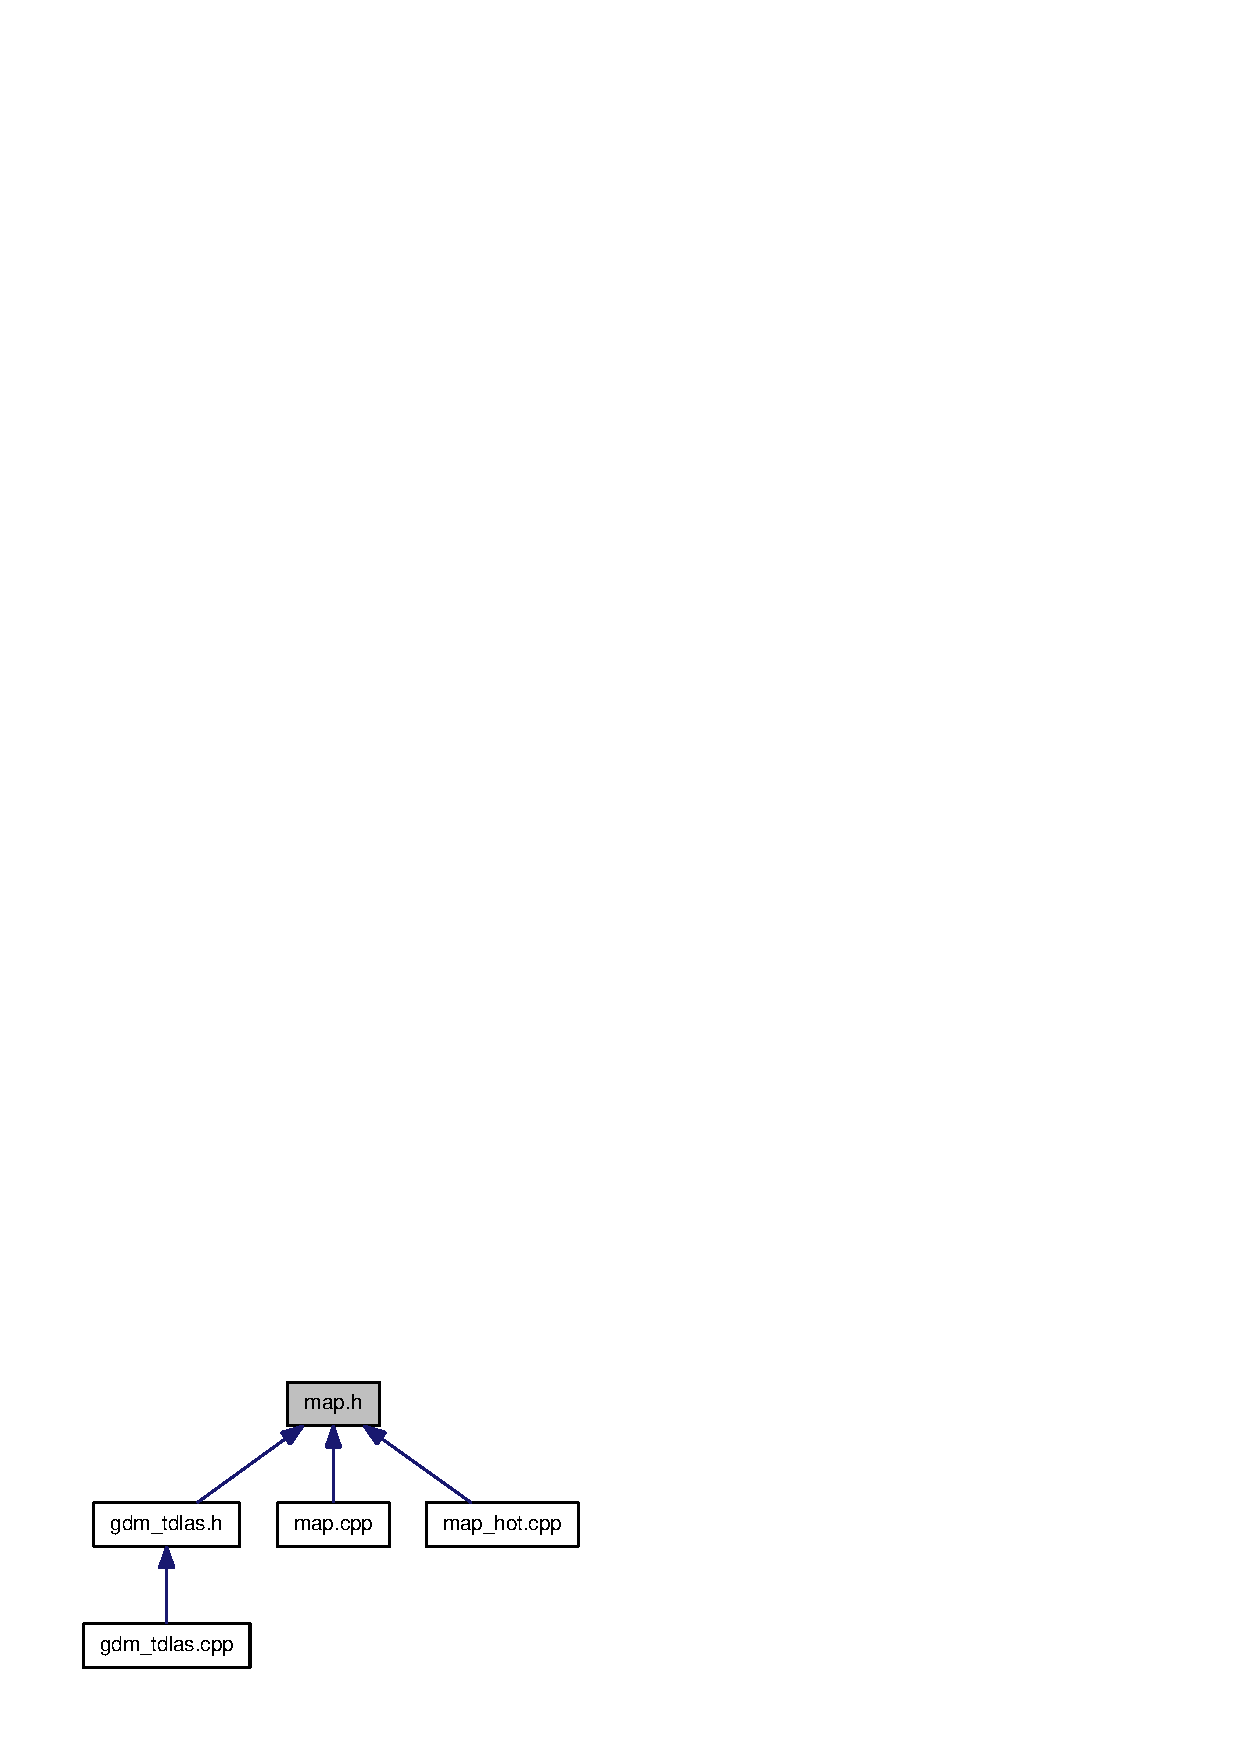
\includegraphics[width=281pt]{map_8h__dep__incl}
\end{center}
\end{figure}
\subsection*{Classes}
\begin{DoxyCompactItemize}
\item 
class {\bf GdmTDLAS::GasMap}
\item 
class {\bf GdmTDLAS::Intersection}
\end{DoxyCompactItemize}
\subsection*{Namespaces}
\begin{DoxyCompactItemize}
\item 
namespace {\bf GdmTDLAS}
\end{DoxyCompactItemize}
\subsection*{Variables}
\begin{DoxyCompactItemize}
\item 
static const float {\bf blue} [64] = \{1.0000,0.9861,0.9722,0.9583,0.9444,0.9306,0.9167,0.9028,0.8889,0.8750,0.8611,0.8472,0.8333,0.8194,0.8056,0.7917,0.7778,0.7639,0.7500,0.7361,0.7222,0.7083,0.6944,0.6806,0.6667,0.6528,0.6389,0.6250,0.6111,0.5972,0.5833,0.5694,0.5556,0.5417,0.5278,0.5139,0.5000,0.4861,0.4722,0.4583,0.4444,0.4253,0.4062,0.3872,0.3681,0.3490,0.3299,0.3108,0.2917,0.2726,0.2535,0.2344,0.2153,0.1962,0.1771,0.1580,0.1389,0.1198,0.1007,0.0816,0.0625,0.0434,0.0243,0.0052\}
\item 
static const float {\bf green} [64] = \{1.0000,0.9861,0.9722,0.9583,0.9444,0.9306,0.9167,0.9028,0.8889,0.8750,0.8611,0.8472,0.8333,0.8194,0.8056,0.7917,0.7778,0.7587,0.7396,0.7205,0.7014,0.6823,0.6632,0.6441,0.6250,0.6059,0.5868,0.5677,0.5486,0.5295,0.5104,0.4913,0.4722,0.4531,0.4340,0.4149,0.3958,0.3767,0.3576,0.3385,0.3194,0.3056,0.2917,0.2778,0.2639,0.2500,0.2361,0.2222,0.2083,0.1944,0.1806,0.1667,0.1528,0.1389,0.1250,0.1111,0.0972,0.0833,0.0694,0.0556,0.0417,0.0278,0.0139,0\}
\item 
static const float {\bf red} [64] = \{1.0000,0.9783,0.9566,0.9349,0.9132,0.8915,0.8698,0.8481,0.8264,0.8047,0.7830,0.7613,0.7396,0.7179,0.6962,0.6745,0.6528,0.6389,0.6250,0.6111,0.5972,0.5833,0.5694,0.5556,0.5417,0.5278,0.5139,0.5000,0.4861,0.4722,0.4583,0.4444,0.4306,0.4167,0.4028,0.3889,0.3750,0.3611,0.3472,0.3333,0.3194,0.3056,0.2917,0.2778,0.2639,0.2500,0.2361,0.2222,0.2083,0.1944,0.1806,0.1667,0.1528,0.1389,0.1250,0.1111,0.0972,0.0833,0.0694,0.0556,0.0417,0.0278,0.0139,0\}
\end{DoxyCompactItemize}


\subsection{Variable Documentation}
\index{map.h@{map.h}!blue@{blue}}
\index{blue@{blue}!map.h@{map.h}}
\subsubsection[{blue}]{\setlength{\rightskip}{0pt plus 5cm}const float {\bf blue}[64] = \{1.0000,0.9861,0.9722,0.9583,0.9444,0.9306,0.9167,0.9028,0.8889,0.8750,0.8611,0.8472,0.8333,0.8194,0.8056,0.7917,0.7778,0.7639,0.7500,0.7361,0.7222,0.7083,0.6944,0.6806,0.6667,0.6528,0.6389,0.6250,0.6111,0.5972,0.5833,0.5694,0.5556,0.5417,0.5278,0.5139,0.5000,0.4861,0.4722,0.4583,0.4444,0.4253,0.4062,0.3872,0.3681,0.3490,0.3299,0.3108,0.2917,0.2726,0.2535,0.2344,0.2153,0.1962,0.1771,0.1580,0.1389,0.1198,0.1007,0.0816,0.0625,0.0434,0.0243,0.0052\}\hspace{0.3cm}{\ttfamily  [static]}}\label{map_8h_a994a56fa1d2480380394586f82922c7a}


Definition at line 113 of file map.h.

\index{map.h@{map.h}!green@{green}}
\index{green@{green}!map.h@{map.h}}
\subsubsection[{green}]{\setlength{\rightskip}{0pt plus 5cm}const float {\bf green}[64] = \{1.0000,0.9861,0.9722,0.9583,0.9444,0.9306,0.9167,0.9028,0.8889,0.8750,0.8611,0.8472,0.8333,0.8194,0.8056,0.7917,0.7778,0.7587,0.7396,0.7205,0.7014,0.6823,0.6632,0.6441,0.6250,0.6059,0.5868,0.5677,0.5486,0.5295,0.5104,0.4913,0.4722,0.4531,0.4340,0.4149,0.3958,0.3767,0.3576,0.3385,0.3194,0.3056,0.2917,0.2778,0.2639,0.2500,0.2361,0.2222,0.2083,0.1944,0.1806,0.1667,0.1528,0.1389,0.1250,0.1111,0.0972,0.0833,0.0694,0.0556,0.0417,0.0278,0.0139,0\}\hspace{0.3cm}{\ttfamily  [static]}}\label{map_8h_a540851e576db993bc651f251fab01028}


Definition at line 112 of file map.h.

\index{map.h@{map.h}!red@{red}}
\index{red@{red}!map.h@{map.h}}
\subsubsection[{red}]{\setlength{\rightskip}{0pt plus 5cm}const float {\bf red}[64] = \{1.0000,0.9783,0.9566,0.9349,0.9132,0.8915,0.8698,0.8481,0.8264,0.8047,0.7830,0.7613,0.7396,0.7179,0.6962,0.6745,0.6528,0.6389,0.6250,0.6111,0.5972,0.5833,0.5694,0.5556,0.5417,0.5278,0.5139,0.5000,0.4861,0.4722,0.4583,0.4444,0.4306,0.4167,0.4028,0.3889,0.3750,0.3611,0.3472,0.3333,0.3194,0.3056,0.2917,0.2778,0.2639,0.2500,0.2361,0.2222,0.2083,0.1944,0.1806,0.1667,0.1528,0.1389,0.1250,0.1111,0.0972,0.0833,0.0694,0.0556,0.0417,0.0278,0.0139,0\}\hspace{0.3cm}{\ttfamily  [static]}}\label{map_8h_a7aa1e993dd4e98d7f56db1534eb6c462}


Definition at line 111 of file map.h.


\section{map\_\-hot.cpp File Reference}
\label{map__hot_8cpp}\index{map\_\-hot.cpp@{map\_\-hot.cpp}}
{\ttfamily \#include \char`\"{}map.h\char`\"{}}\par
{\ttfamily \#include \char`\"{}math.h\char`\"{}}\par
Include dependency graph for map\_\-hot.cpp:
\nopagebreak
\begin{figure}[H]
\begin{center}
\leavevmode
\includegraphics[width=400pt]{map__hot_8cpp__incl}
\end{center}
\end{figure}

\input{map__hot_8h}
\section{Matrices.cpp File Reference}
\label{Matrices_8cpp}\index{Matrices.cpp@{Matrices.cpp}}
{\ttfamily \#include $<$qpOASES.hpp$>$}\par
Include dependency graph for Matrices.cpp:
\nopagebreak
\begin{figure}[H]
\begin{center}
\leavevmode
\includegraphics[width=400pt]{Matrices_8cpp__incl}
\end{center}
\end{figure}
\subsection*{Variables}
\begin{DoxyCompactItemize}
\item 
const char $\ast$const {\bf NOTRANS} = \char`\"{}NOTRANS\char`\"{}
\item 
BEGIN\_\-NAMESPACE\_\-QPOASES const char $\ast$const {\bf TRANS} = \char`\"{}TRANS\char`\"{}
\end{DoxyCompactItemize}


\subsection{Detailed Description}
\begin{DoxyAuthor}{Author}
Hans Joachim Ferreau, Andreas Potschka, Christian Kirches 
\end{DoxyAuthor}
\begin{DoxyVersion}{Version}
3.0beta 
\end{DoxyVersion}
\begin{DoxyDate}{Date}
2007-\/2012
\end{DoxyDate}
Implementation of the matrix classes. 

Definition in file {\bf Matrices.cpp}.



\subsection{Variable Documentation}
\index{Matrices.cpp@{Matrices.cpp}!NOTRANS@{NOTRANS}}
\index{NOTRANS@{NOTRANS}!Matrices.cpp@{Matrices.cpp}}
\subsubsection[{NOTRANS}]{\setlength{\rightskip}{0pt plus 5cm}const char$\ast$ const {\bf NOTRANS} = \char`\"{}NOTRANS\char`\"{}}\label{Matrices_8cpp_a36a7cf4c2c0701885198a994a267966c}
String for calling LAPACK/BLAS routines without transposing the matrix. 

Definition at line 44 of file Matrices.cpp.

\index{Matrices.cpp@{Matrices.cpp}!TRANS@{TRANS}}
\index{TRANS@{TRANS}!Matrices.cpp@{Matrices.cpp}}
\subsubsection[{TRANS}]{\setlength{\rightskip}{0pt plus 5cm}BEGIN\_\-NAMESPACE\_\-QPOASES const char$\ast$ const {\bf TRANS} = \char`\"{}TRANS\char`\"{}}\label{Matrices_8cpp_a4b6e2a35d324bb658c4d391cedbb7225}
String for calling LAPACK/BLAS routines with transposed matrices. 

Definition at line 41 of file Matrices.cpp.


\section{Matrices.hpp File Reference}
\label{Matrices_8hpp}\index{Matrices.hpp@{Matrices.hpp}}
This graph shows which files directly or indirectly include this file:
\nopagebreak
\begin{figure}[H]
\begin{center}
\leavevmode
\includegraphics[width=400pt]{Matrices_8hpp__dep__incl}
\end{center}
\end{figure}
\subsection*{Classes}
\begin{DoxyCompactItemize}
\item 
class {\bf DenseMatrix}
\begin{DoxyCompactList}\small\item\em Interfaces matrix-\/vector operations tailored to general dense matrices. \end{DoxyCompactList}\item 
class {\bf Matrix}
\begin{DoxyCompactList}\small\item\em Abstract base class for interfacing tailored matrix-\/vector operations. \end{DoxyCompactList}\item 
class {\bf SparseMatrix}
\begin{DoxyCompactList}\small\item\em Interfaces matrix-\/vector operations tailored to general sparse matrices. \end{DoxyCompactList}\item 
class {\bf SparseMatrixRow}
\begin{DoxyCompactList}\small\item\em Interfaces matrix-\/vector operations tailored to general sparse matrices. \end{DoxyCompactList}\item 
class {\bf SymDenseMat}
\begin{DoxyCompactList}\small\item\em Interfaces matrix-\/vector operations tailored to symmetric dense matrices. \end{DoxyCompactList}\item 
class {\bf SymmetricMatrix}
\begin{DoxyCompactList}\small\item\em Abstract base class for interfacing matrix-\/vector operations tailored to symmetric matrices. \end{DoxyCompactList}\item 
class {\bf SymSparseMat}
\begin{DoxyCompactList}\small\item\em Interfaces matrix-\/vector operations tailored to symmetric sparse matrices. \end{DoxyCompactList}\end{DoxyCompactItemize}
\subsection*{Defines}
\begin{DoxyCompactItemize}
\item 
\#define {\bf GEMM}~dgemm\_\-
\item 
\#define {\bf POTRF}~dpotrf\_\-
\item 
\#define {\bf SYR}~dsyr\_\-
\item 
\#define {\bf SYR2}~dsyr2\_\-
\end{DoxyCompactItemize}
\subsection*{Functions}
\begin{DoxyCompactItemize}
\item 
void {\bf dgemm\_\-} (const char $\ast$, const char $\ast$, const unsigned long $\ast$, const unsigned long $\ast$, const unsigned long $\ast$, const double $\ast$, const double $\ast$, const unsigned long $\ast$, const double $\ast$, const unsigned long $\ast$, const double $\ast$, double $\ast$, const unsigned long $\ast$)
\item 
void {\bf dpotrf\_\-} (const char $\ast$, const unsigned long $\ast$, double $\ast$, const unsigned long $\ast$, long $\ast$)
\item 
void {\bf dsyr2\_\-} (const char $\ast$, const unsigned long $\ast$, const double $\ast$, const double $\ast$, const unsigned long $\ast$, const double $\ast$, const unsigned long $\ast$, double $\ast$, const unsigned long $\ast$)
\item 
void {\bf dsyr\_\-} (const char $\ast$, const unsigned long $\ast$, const double $\ast$, const double $\ast$, const unsigned long $\ast$, double $\ast$, const unsigned long $\ast$)
\item 
void {\bf sgemm\_\-} (const char $\ast$, const char $\ast$, const unsigned long $\ast$, const unsigned long $\ast$, const unsigned long $\ast$, const float $\ast$, const float $\ast$, const unsigned long $\ast$, const float $\ast$, const unsigned long $\ast$, const float $\ast$, float $\ast$, const unsigned long $\ast$)
\item 
void {\bf spotrf\_\-} (const char $\ast$, const unsigned long $\ast$, float $\ast$, const unsigned long $\ast$, long $\ast$)
\item 
void {\bf ssyr2\_\-} (const char $\ast$, const unsigned long $\ast$, const float $\ast$, const float $\ast$, const unsigned long $\ast$, const float $\ast$, const unsigned long $\ast$, float $\ast$, const unsigned long $\ast$)
\item 
void {\bf ssyr\_\-} (const char $\ast$, const unsigned long $\ast$, const float $\ast$, const float $\ast$, const unsigned long $\ast$, float $\ast$, const unsigned long $\ast$)
\end{DoxyCompactItemize}
\subsection*{Variables}
\begin{DoxyCompactItemize}
\item 
BEGIN\_\-NAMESPACE\_\-QPOASES typedef int {\bf sparse\_\-int\_\-t}
\end{DoxyCompactItemize}


\subsection{Detailed Description}
\begin{DoxyAuthor}{Author}
Hans Joachim Ferreau, Andreas Potschka, Christian Kirches 
\end{DoxyAuthor}
\begin{DoxyVersion}{Version}
3.0beta 
\end{DoxyVersion}
\begin{DoxyDate}{Date}
2009-\/2012
\end{DoxyDate}
Various matrix classes: Abstract base matrix class, dense and sparse matrices, including symmetry exploiting specializations. 

Definition in file {\bf Matrices.hpp}.



\subsection{Define Documentation}
\index{Matrices.hpp@{Matrices.hpp}!GEMM@{GEMM}}
\index{GEMM@{GEMM}!Matrices.hpp@{Matrices.hpp}}
\subsubsection[{GEMM}]{\setlength{\rightskip}{0pt plus 5cm}\#define GEMM~dgemm\_\-}\label{Matrices_8hpp_a68c6925602a91b3f1b335f64f533350c}
Macro for calling level 3 BLAS operation in double precision. 

Definition at line 55 of file Matrices.hpp.

\index{Matrices.hpp@{Matrices.hpp}!POTRF@{POTRF}}
\index{POTRF@{POTRF}!Matrices.hpp@{Matrices.hpp}}
\subsubsection[{POTRF}]{\setlength{\rightskip}{0pt plus 5cm}\#define POTRF~dpotrf\_\-}\label{Matrices_8hpp_a39fd888b29dc1aba3c780981acdd7f62}
Macro for calling level 3 BLAS operation in double precision. 

Definition at line 61 of file Matrices.hpp.

\index{Matrices.hpp@{Matrices.hpp}!SYR@{SYR}}
\index{SYR@{SYR}!Matrices.hpp@{Matrices.hpp}}
\subsubsection[{SYR}]{\setlength{\rightskip}{0pt plus 5cm}\#define SYR~dsyr\_\-}\label{Matrices_8hpp_a5ee0a497d3653585eb12da8940842993}
Macro for calling level 3 BLAS operation in double precision. 

Definition at line 57 of file Matrices.hpp.

\index{Matrices.hpp@{Matrices.hpp}!SYR2@{SYR2}}
\index{SYR2@{SYR2}!Matrices.hpp@{Matrices.hpp}}
\subsubsection[{SYR2}]{\setlength{\rightskip}{0pt plus 5cm}\#define SYR2~dsyr2\_\-}\label{Matrices_8hpp_a5f81ee60143e803bb030c1180cd8ec5a}
Macro for calling level 3 BLAS operation in double precision. 

Definition at line 59 of file Matrices.hpp.



\subsection{Function Documentation}
\index{Matrices.hpp@{Matrices.hpp}!dgemm\_\-@{dgemm\_\-}}
\index{dgemm\_\-@{dgemm\_\-}!Matrices.hpp@{Matrices.hpp}}
\subsubsection[{dgemm\_\-}]{\setlength{\rightskip}{0pt plus 5cm}void dgemm\_\- (
\begin{DoxyParamCaption}
\item[{const char $\ast$}]{, }
\item[{const char $\ast$}]{, }
\item[{const unsigned long $\ast$}]{, }
\item[{const unsigned long $\ast$}]{, }
\item[{const unsigned long $\ast$}]{, }
\item[{const double $\ast$}]{, }
\item[{const double $\ast$}]{, }
\item[{const unsigned long $\ast$}]{, }
\item[{const double $\ast$}]{, }
\item[{const unsigned long $\ast$}]{, }
\item[{const double $\ast$}]{, }
\item[{double $\ast$}]{, }
\item[{const unsigned long $\ast$}]{}
\end{DoxyParamCaption}
)}\label{Matrices_8hpp_abc759a939c9e9258abfc2f558f78c87f}
Performs one of the matrix-\/matrix operation in double precision. 

Definition at line 36 of file BLASReplacement.cpp.

\index{Matrices.hpp@{Matrices.hpp}!dpotrf\_\-@{dpotrf\_\-}}
\index{dpotrf\_\-@{dpotrf\_\-}!Matrices.hpp@{Matrices.hpp}}
\subsubsection[{dpotrf\_\-}]{\setlength{\rightskip}{0pt plus 5cm}void dpotrf\_\- (
\begin{DoxyParamCaption}
\item[{const char $\ast$}]{, }
\item[{const unsigned long $\ast$}]{, }
\item[{double $\ast$}]{, }
\item[{const unsigned long $\ast$}]{, }
\item[{long $\ast$}]{}
\end{DoxyParamCaption}
)}\label{Matrices_8hpp_a5bad6f61c16311987c9286e9bb161006}
Calculates the Cholesky factorization of a real symmetric positive definite matrix in double precision. 

Definition at line 38 of file LAPACKReplacement.cpp.

\index{Matrices.hpp@{Matrices.hpp}!dsyr2\_\-@{dsyr2\_\-}}
\index{dsyr2\_\-@{dsyr2\_\-}!Matrices.hpp@{Matrices.hpp}}
\subsubsection[{dsyr2\_\-}]{\setlength{\rightskip}{0pt plus 5cm}void dsyr2\_\- (
\begin{DoxyParamCaption}
\item[{const char $\ast$}]{, }
\item[{const unsigned long $\ast$}]{, }
\item[{const double $\ast$}]{, }
\item[{const double $\ast$}]{, }
\item[{const unsigned long $\ast$}]{, }
\item[{const double $\ast$}]{, }
\item[{const unsigned long $\ast$}]{, }
\item[{double $\ast$}]{, }
\item[{const unsigned long $\ast$}]{}
\end{DoxyParamCaption}
)}\label{Matrices_8hpp_a706f3b03c33ac58d31c681d7faf6fedf}
Performs a symmetric rank 2 operation in double precision. \index{Matrices.hpp@{Matrices.hpp}!dsyr\_\-@{dsyr\_\-}}
\index{dsyr\_\-@{dsyr\_\-}!Matrices.hpp@{Matrices.hpp}}
\subsubsection[{dsyr\_\-}]{\setlength{\rightskip}{0pt plus 5cm}void dsyr\_\- (
\begin{DoxyParamCaption}
\item[{const char $\ast$}]{, }
\item[{const unsigned long $\ast$}]{, }
\item[{const double $\ast$}]{, }
\item[{const double $\ast$}]{, }
\item[{const unsigned long $\ast$}]{, }
\item[{double $\ast$}]{, }
\item[{const unsigned long $\ast$}]{}
\end{DoxyParamCaption}
)}\label{Matrices_8hpp_aa487bf28ac0323a6b12c5ad95b69a5a2}
Performs a symmetric rank 1 operation in double precision. \index{Matrices.hpp@{Matrices.hpp}!sgemm\_\-@{sgemm\_\-}}
\index{sgemm\_\-@{sgemm\_\-}!Matrices.hpp@{Matrices.hpp}}
\subsubsection[{sgemm\_\-}]{\setlength{\rightskip}{0pt plus 5cm}void sgemm\_\- (
\begin{DoxyParamCaption}
\item[{const char $\ast$}]{, }
\item[{const char $\ast$}]{, }
\item[{const unsigned long $\ast$}]{, }
\item[{const unsigned long $\ast$}]{, }
\item[{const unsigned long $\ast$}]{, }
\item[{const float $\ast$}]{, }
\item[{const float $\ast$}]{, }
\item[{const unsigned long $\ast$}]{, }
\item[{const float $\ast$}]{, }
\item[{const unsigned long $\ast$}]{, }
\item[{const float $\ast$}]{, }
\item[{float $\ast$}]{, }
\item[{const unsigned long $\ast$}]{}
\end{DoxyParamCaption}
)}\label{Matrices_8hpp_a2d0404fd005dbb78f314e48e46dc14f2}
Performs one of the matrix-\/matrix operation in single precision. 

Definition at line 90 of file BLASReplacement.cpp.

\index{Matrices.hpp@{Matrices.hpp}!spotrf\_\-@{spotrf\_\-}}
\index{spotrf\_\-@{spotrf\_\-}!Matrices.hpp@{Matrices.hpp}}
\subsubsection[{spotrf\_\-}]{\setlength{\rightskip}{0pt plus 5cm}void spotrf\_\- (
\begin{DoxyParamCaption}
\item[{const char $\ast$}]{, }
\item[{const unsigned long $\ast$}]{, }
\item[{float $\ast$}]{, }
\item[{const unsigned long $\ast$}]{, }
\item[{long $\ast$}]{}
\end{DoxyParamCaption}
)}\label{Matrices_8hpp_a519c3855d35f97aeeb2b8e583846c2f0}
Calculates the Cholesky factorization of a real symmetric positive definite matrix in single precision. \index{Matrices.hpp@{Matrices.hpp}!ssyr2\_\-@{ssyr2\_\-}}
\index{ssyr2\_\-@{ssyr2\_\-}!Matrices.hpp@{Matrices.hpp}}
\subsubsection[{ssyr2\_\-}]{\setlength{\rightskip}{0pt plus 5cm}void ssyr2\_\- (
\begin{DoxyParamCaption}
\item[{const char $\ast$}]{, }
\item[{const unsigned long $\ast$}]{, }
\item[{const float $\ast$}]{, }
\item[{const float $\ast$}]{, }
\item[{const unsigned long $\ast$}]{, }
\item[{const float $\ast$}]{, }
\item[{const unsigned long $\ast$}]{, }
\item[{float $\ast$}]{, }
\item[{const unsigned long $\ast$}]{}
\end{DoxyParamCaption}
)}\label{Matrices_8hpp_a42495df75d1c4859ee2f7a4a3d7f57ca}
Performs a symmetric rank 2 operation in single precision. \index{Matrices.hpp@{Matrices.hpp}!ssyr\_\-@{ssyr\_\-}}
\index{ssyr\_\-@{ssyr\_\-}!Matrices.hpp@{Matrices.hpp}}
\subsubsection[{ssyr\_\-}]{\setlength{\rightskip}{0pt plus 5cm}void ssyr\_\- (
\begin{DoxyParamCaption}
\item[{const char $\ast$}]{, }
\item[{const unsigned long $\ast$}]{, }
\item[{const float $\ast$}]{, }
\item[{const float $\ast$}]{, }
\item[{const unsigned long $\ast$}]{, }
\item[{float $\ast$}]{, }
\item[{const unsigned long $\ast$}]{}
\end{DoxyParamCaption}
)}\label{Matrices_8hpp_a8c9fdafb90f8718c2ce7febbb4c72f2f}
Performs a symmetric rank 1 operation in single precision. 

\subsection{Variable Documentation}
\index{Matrices.hpp@{Matrices.hpp}!sparse\_\-int\_\-t@{sparse\_\-int\_\-t}}
\index{sparse\_\-int\_\-t@{sparse\_\-int\_\-t}!Matrices.hpp@{Matrices.hpp}}
\subsubsection[{sparse\_\-int\_\-t}]{\setlength{\rightskip}{0pt plus 5cm}BEGIN\_\-NAMESPACE\_\-QPOASES typedef int {\bf sparse\_\-int\_\-t}}\label{Matrices_8hpp_a0cc0f6e829c2163b8479d91190252d7d}


Definition at line 106 of file Matrices.hpp.


\section{MessageHandling.cpp File Reference}
\label{MessageHandling_8cpp}\index{MessageHandling.cpp@{MessageHandling.cpp}}
{\ttfamily \#include $<$stdio.h$>$}\par
{\ttfamily \#include $<$qpOASES/MessageHandling.hpp$>$}\par
{\ttfamily \#include $<$qpOASES/Utils.hpp$>$}\par
Include dependency graph for MessageHandling.cpp:
\nopagebreak
\begin{figure}[H]
\begin{center}
\leavevmode
\includegraphics[width=400pt]{MessageHandling_8cpp__incl}
\end{center}
\end{figure}
\subsection*{Functions}
\begin{DoxyCompactItemize}
\item 
{\bf MessageHandling} $\ast$ {\bf getGlobalMessageHandler} ()
\end{DoxyCompactItemize}
\subsection*{Variables}
\begin{DoxyCompactItemize}
\item 
{\bf MessageHandling} {\bf globalMessageHandler} (stderr, VS\_\-VISIBLE, VS\_\-VISIBLE, VS\_\-VISIBLE)
\item 
BEGIN\_\-NAMESPACE\_\-QPOASES {\bf MessageHandling::ReturnValueList} {\bf returnValueList} [$\,$]
\end{DoxyCompactItemize}


\subsection{Detailed Description}
\begin{DoxyAuthor}{Author}
Hans Joachim Ferreau, Andreas Potschka, Christian Kirches 
\end{DoxyAuthor}
\begin{DoxyVersion}{Version}
3.0beta 
\end{DoxyVersion}
\begin{DoxyDate}{Date}
2007-\/2012
\end{DoxyDate}
Implementation of the \doxyref{MessageHandling}{p.}{classMessageHandling} class including global return values. 

Definition in file {\bf MessageHandling.cpp}.



\subsection{Function Documentation}
\index{MessageHandling.cpp@{MessageHandling.cpp}!getGlobalMessageHandler@{getGlobalMessageHandler}}
\index{getGlobalMessageHandler@{getGlobalMessageHandler}!MessageHandling.cpp@{MessageHandling.cpp}}
\subsubsection[{getGlobalMessageHandler}]{\setlength{\rightskip}{0pt plus 5cm}{\bf MessageHandling}$\ast$ getGlobalMessageHandler (
\begin{DoxyParamCaption}
{}
\end{DoxyParamCaption}
)}\label{MessageHandling_8cpp_aaa22c4eae12c4dd65bdb0459ba26e372}
Returns a pointer to global message handler. \begin{DoxyReturn}{Returns}
Pointer to global message handler. 
\end{DoxyReturn}


Definition at line 565 of file MessageHandling.cpp.



\subsection{Variable Documentation}
\index{MessageHandling.cpp@{MessageHandling.cpp}!globalMessageHandler@{globalMessageHandler}}
\index{globalMessageHandler@{globalMessageHandler}!MessageHandling.cpp@{MessageHandling.cpp}}
\subsubsection[{globalMessageHandler}]{\setlength{\rightskip}{0pt plus 5cm}{\bf MessageHandling} {\bf globalMessageHandler}(stderr, VS\_\-VISIBLE, VS\_\-VISIBLE, VS\_\-VISIBLE)}\label{MessageHandling_8cpp_af96b913fc115550a6433662158595076}
Global message handler for all qpOASES modules. \index{MessageHandling.cpp@{MessageHandling.cpp}!returnValueList@{returnValueList}}
\index{returnValueList@{returnValueList}!MessageHandling.cpp@{MessageHandling.cpp}}
\subsubsection[{returnValueList}]{\setlength{\rightskip}{0pt plus 5cm}BEGIN\_\-NAMESPACE\_\-QPOASES {\bf MessageHandling::ReturnValueList} {\bf returnValueList}[$\,$]}\label{MessageHandling_8cpp_abb2efff5764a2a8ec555b59f453d8485}
Defines pairs of global return values and messages. 

Definition at line 51 of file MessageHandling.cpp.


\section{MessageHandling.hpp File Reference}
\label{MessageHandling_8hpp}\index{MessageHandling.hpp@{MessageHandling.hpp}}
{\ttfamily \#include $<$stdio.h$>$}\par
{\ttfamily \#include $<$string.h$>$}\par
{\ttfamily \#include $<$qpOASES/Constants.hpp$>$}\par
{\ttfamily \#include $<$qpOASES/MessageHandling.ipp$>$}\par
Include dependency graph for MessageHandling.hpp:
\nopagebreak
\begin{figure}[H]
\begin{center}
\leavevmode
\includegraphics[width=400pt]{MessageHandling_8hpp__incl}
\end{center}
\end{figure}
This graph shows which files directly or indirectly include this file:
\nopagebreak
\begin{figure}[H]
\begin{center}
\leavevmode
\includegraphics[width=400pt]{MessageHandling_8hpp__dep__incl}
\end{center}
\end{figure}
\subsection*{Classes}
\begin{DoxyCompactItemize}
\item 
class {\bf MessageHandling}
\begin{DoxyCompactList}\small\item\em Handles all kind of error messages, warnings and other information. \end{DoxyCompactList}\item 
struct {\bf MessageHandling::ReturnValueList}
\begin{DoxyCompactList}\small\item\em Data structure for entries in global message list. \end{DoxyCompactList}\end{DoxyCompactItemize}
\subsection*{Defines}
\begin{DoxyCompactItemize}
\item 
\#define {\bf \_\-\_\-FILE\_\-\_\-}~0
\item 
\#define {\bf \_\-\_\-FUNCTION\_\-\_\-}~0
\item 
\#define {\bf \_\-\_\-LINE\_\-\_\-}~0
\item 
\#define {\bf THROWERROR}(retval)~( getGlobalMessageHandler( )-\/$>$throwError((retval),0,\_\-\_\-FUNCTION\_\-\_\-,\_\-\_\-FILE\_\-\_\-,\_\-\_\-LINE\_\-\_\-,VS\_\-VISIBLE) )
\item 
\#define {\bf THROWINFO}(retval)~( getGlobalMessageHandler( )-\/$>$throwInfo((retval),0,\_\-\_\-FUNCTION\_\-\_\-,\_\-\_\-FILE\_\-\_\-,\_\-\_\-LINE\_\-\_\-,VS\_\-VISIBLE) )
\item 
\#define {\bf THROWWARNING}(retval)~( getGlobalMessageHandler( )-\/$>$throwWarning((retval),0,\_\-\_\-FUNCTION\_\-\_\-,\_\-\_\-FILE\_\-\_\-,\_\-\_\-LINE\_\-\_\-,VS\_\-VISIBLE) )
\end{DoxyCompactItemize}
\subsection*{Enumerations}
\begin{DoxyCompactItemize}
\item 
enum {\bf returnValue} \{ \par
{\bf TERMINAL\_\-LIST\_\-ELEMENT} =  -\/1, 
{\bf SUCCESSFUL\_\-RETURN} =  0, 
{\bf RET\_\-DIV\_\-BY\_\-ZERO}, 
{\bf RET\_\-INDEX\_\-OUT\_\-OF\_\-BOUNDS}, 
\par
{\bf RET\_\-INVALID\_\-ARGUMENTS}, 
{\bf RET\_\-ERROR\_\-UNDEFINED}, 
{\bf RET\_\-WARNING\_\-UNDEFINED}, 
{\bf RET\_\-INFO\_\-UNDEFINED}, 
\par
{\bf RET\_\-EWI\_\-UNDEFINED}, 
{\bf RET\_\-AVAILABLE\_\-WITH\_\-LINUX\_\-ONLY}, 
{\bf RET\_\-UNKNOWN\_\-BUG}, 
{\bf RET\_\-PRINTLEVEL\_\-CHANGED}, 
\par
{\bf RET\_\-NOT\_\-YET\_\-IMPLEMENTED}, 
{\bf RET\_\-INDEXLIST\_\-MUST\_\-BE\_\-REORDERD}, 
{\bf RET\_\-INDEXLIST\_\-EXCEEDS\_\-MAX\_\-LENGTH}, 
{\bf RET\_\-INDEXLIST\_\-CORRUPTED}, 
\par
{\bf RET\_\-INDEXLIST\_\-OUTOFBOUNDS}, 
{\bf RET\_\-INDEXLIST\_\-ADD\_\-FAILED}, 
{\bf RET\_\-INDEXLIST\_\-INTERSECT\_\-FAILED}, 
{\bf RET\_\-INDEX\_\-ALREADY\_\-OF\_\-DESIRED\_\-STATUS}, 
\par
{\bf RET\_\-ADDINDEX\_\-FAILED}, 
{\bf RET\_\-REMOVEINDEX\_\-FAILED}, 
{\bf RET\_\-SWAPINDEX\_\-FAILED}, 
{\bf RET\_\-NOTHING\_\-TO\_\-DO}, 
\par
{\bf RET\_\-SETUP\_\-BOUND\_\-FAILED}, 
{\bf RET\_\-SETUP\_\-CONSTRAINT\_\-FAILED}, 
{\bf RET\_\-MOVING\_\-BOUND\_\-FAILED}, 
{\bf RET\_\-MOVING\_\-CONSTRAINT\_\-FAILED}, 
\par
{\bf RET\_\-SHIFTING\_\-FAILED}, 
{\bf RET\_\-ROTATING\_\-FAILED}, 
{\bf RET\_\-QPOBJECT\_\-NOT\_\-SETUP}, 
{\bf RET\_\-QP\_\-ALREADY\_\-INITIALISED}, 
\par
{\bf RET\_\-NO\_\-INIT\_\-WITH\_\-STANDARD\_\-SOLVER}, 
{\bf RET\_\-RESET\_\-FAILED}, 
{\bf RET\_\-INIT\_\-FAILED}, 
{\bf RET\_\-INIT\_\-FAILED\_\-TQ}, 
\par
{\bf RET\_\-INIT\_\-FAILED\_\-CHOLESKY}, 
{\bf RET\_\-INIT\_\-FAILED\_\-HOTSTART}, 
{\bf RET\_\-INIT\_\-FAILED\_\-INFEASIBILITY}, 
{\bf RET\_\-INIT\_\-FAILED\_\-UNBOUNDEDNESS}, 
\par
{\bf RET\_\-INIT\_\-FAILED\_\-REGULARISATION}, 
{\bf RET\_\-INIT\_\-SUCCESSFUL}, 
{\bf RET\_\-OBTAINING\_\-WORKINGSET\_\-FAILED}, 
{\bf RET\_\-SETUP\_\-WORKINGSET\_\-FAILED}, 
\par
{\bf RET\_\-SETUP\_\-AUXILIARYQP\_\-FAILED}, 
{\bf RET\_\-NO\_\-EXTERN\_\-SOLVER}, 
{\bf RET\_\-QP\_\-UNBOUNDED}, 
{\bf RET\_\-QP\_\-INFEASIBLE}, 
\par
{\bf RET\_\-QP\_\-NOT\_\-SOLVED}, 
{\bf RET\_\-QP\_\-SOLVED}, 
{\bf RET\_\-UNABLE\_\-TO\_\-SOLVE\_\-QP}, 
{\bf RET\_\-INITIALISATION\_\-STARTED}, 
\par
{\bf RET\_\-HOTSTART\_\-FAILED}, 
{\bf RET\_\-HOTSTART\_\-FAILED\_\-TO\_\-INIT}, 
{\bf RET\_\-HOTSTART\_\-FAILED\_\-AS\_\-QP\_\-NOT\_\-INITIALISED}, 
{\bf RET\_\-ITERATION\_\-STARTED}, 
\par
{\bf RET\_\-SHIFT\_\-DETERMINATION\_\-FAILED}, 
{\bf RET\_\-STEPDIRECTION\_\-DETERMINATION\_\-FAILED}, 
{\bf RET\_\-STEPLENGTH\_\-DETERMINATION\_\-FAILED}, 
{\bf RET\_\-OPTIMAL\_\-SOLUTION\_\-FOUND}, 
\par
{\bf RET\_\-HOMOTOPY\_\-STEP\_\-FAILED}, 
{\bf RET\_\-HOTSTART\_\-STOPPED\_\-INFEASIBILITY}, 
{\bf RET\_\-HOTSTART\_\-STOPPED\_\-UNBOUNDEDNESS}, 
{\bf RET\_\-WORKINGSET\_\-UPDATE\_\-FAILED}, 
\par
{\bf RET\_\-MAX\_\-NWSR\_\-REACHED}, 
{\bf RET\_\-CONSTRAINTS\_\-NOT\_\-SPECIFIED}, 
{\bf RET\_\-INVALID\_\-FACTORISATION\_\-FLAG}, 
{\bf RET\_\-UNABLE\_\-TO\_\-SAVE\_\-QPDATA}, 
\par
{\bf RET\_\-STEPDIRECTION\_\-FAILED\_\-TQ}, 
{\bf RET\_\-STEPDIRECTION\_\-FAILED\_\-CHOLESKY}, 
{\bf RET\_\-CYCLING\_\-DETECTED}, 
{\bf RET\_\-CYCLING\_\-NOT\_\-RESOLVED}, 
\par
{\bf RET\_\-CYCLING\_\-RESOLVED}, 
{\bf RET\_\-STEPSIZE}, 
{\bf RET\_\-STEPSIZE\_\-NONPOSITIVE}, 
{\bf RET\_\-SETUPSUBJECTTOTYPE\_\-FAILED}, 
\par
{\bf RET\_\-ADDCONSTRAINT\_\-FAILED}, 
{\bf RET\_\-ADDCONSTRAINT\_\-FAILED\_\-INFEASIBILITY}, 
{\bf RET\_\-ADDBOUND\_\-FAILED}, 
{\bf RET\_\-ADDBOUND\_\-FAILED\_\-INFEASIBILITY}, 
\par
{\bf RET\_\-REMOVECONSTRAINT\_\-FAILED}, 
{\bf RET\_\-REMOVEBOUND\_\-FAILED}, 
{\bf RET\_\-REMOVE\_\-FROM\_\-ACTIVESET}, 
{\bf RET\_\-ADD\_\-TO\_\-ACTIVESET}, 
\par
{\bf RET\_\-REMOVE\_\-FROM\_\-ACTIVESET\_\-FAILED}, 
{\bf RET\_\-ADD\_\-TO\_\-ACTIVESET\_\-FAILED}, 
{\bf RET\_\-CONSTRAINT\_\-ALREADY\_\-ACTIVE}, 
{\bf RET\_\-ALL\_\-CONSTRAINTS\_\-ACTIVE}, 
\par
{\bf RET\_\-LINEARLY\_\-DEPENDENT}, 
{\bf RET\_\-LINEARLY\_\-INDEPENDENT}, 
{\bf RET\_\-LI\_\-RESOLVED}, 
{\bf RET\_\-ENSURELI\_\-FAILED}, 
\par
{\bf RET\_\-ENSURELI\_\-FAILED\_\-TQ}, 
{\bf RET\_\-ENSURELI\_\-FAILED\_\-NOINDEX}, 
{\bf RET\_\-ENSURELI\_\-FAILED\_\-CYCLING}, 
{\bf RET\_\-BOUND\_\-ALREADY\_\-ACTIVE}, 
\par
{\bf RET\_\-ALL\_\-BOUNDS\_\-ACTIVE}, 
{\bf RET\_\-CONSTRAINT\_\-NOT\_\-ACTIVE}, 
{\bf RET\_\-BOUND\_\-NOT\_\-ACTIVE}, 
{\bf RET\_\-HESSIAN\_\-NOT\_\-SPD}, 
\par
{\bf RET\_\-HESSIAN\_\-INDEFINITE}, 
{\bf RET\_\-MATRIX\_\-SHIFT\_\-FAILED}, 
{\bf RET\_\-MATRIX\_\-FACTORISATION\_\-FAILED}, 
{\bf RET\_\-PRINT\_\-ITERATION\_\-FAILED}, 
\par
{\bf RET\_\-NO\_\-GLOBAL\_\-MESSAGE\_\-OUTPUTFILE}, 
{\bf RET\_\-DISABLECONSTRAINTS\_\-FAILED}, 
{\bf RET\_\-ENABLECONSTRAINTS\_\-FAILED}, 
{\bf RET\_\-ALREADY\_\-ENABLED}, 
\par
{\bf RET\_\-ALREADY\_\-DISABLED}, 
{\bf RET\_\-NO\_\-HESSIAN\_\-SPECIFIED}, 
{\bf RET\_\-USING\_\-REGULARISATION}, 
{\bf RET\_\-EPS\_\-MUST\_\-BE\_\-POSITVE}, 
\par
{\bf RET\_\-REGSTEPS\_\-MUST\_\-BE\_\-POSITVE}, 
{\bf RET\_\-HESSIAN\_\-ALREADY\_\-REGULARISED}, 
{\bf RET\_\-CANNOT\_\-REGULARISE\_\-IDENTITY}, 
{\bf RET\_\-CANNOT\_\-REGULARISE\_\-SPARSE}, 
\par
{\bf RET\_\-NO\_\-REGSTEP\_\-NWSR}, 
{\bf RET\_\-FEWER\_\-REGSTEPS\_\-NWSR}, 
{\bf RET\_\-CHOLESKY\_\-OF\_\-ZERO\_\-HESSIAN}, 
{\bf RET\_\-CONSTRAINTS\_\-ARE\_\-NOT\_\-SCALED}, 
\par
{\bf RET\_\-ERROR\_\-IN\_\-CONSTRAINTPRODUCT}, 
{\bf RET\_\-UPDATEMATRICES\_\-FAILED}, 
{\bf RET\_\-UPDATEMATRICES\_\-FAILED\_\-AS\_\-QP\_\-NOT\_\-SOLVED}, 
{\bf RET\_\-UNABLE\_\-TO\_\-OPEN\_\-FILE}, 
\par
{\bf RET\_\-UNABLE\_\-TO\_\-WRITE\_\-FILE}, 
{\bf RET\_\-UNABLE\_\-TO\_\-READ\_\-FILE}, 
{\bf RET\_\-FILEDATA\_\-INCONSISTENT}, 
{\bf RET\_\-UNABLE\_\-TO\_\-ANALYSE\_\-QPROBLEM}, 
\par
{\bf RET\_\-NWSR\_\-SET\_\-TO\_\-ONE}, 
{\bf RET\_\-UNABLE\_\-TO\_\-READ\_\-BENCHMARK}, 
{\bf RET\_\-BENCHMARK\_\-ABORTED}, 
{\bf RET\_\-INITIAL\_\-QP\_\-SOLVED}, 
\par
{\bf RET\_\-QP\_\-SOLUTION\_\-STARTED}, 
{\bf RET\_\-BENCHMARK\_\-SUCCESSFUL}, 
{\bf RET\_\-NO\_\-DIAGONAL\_\-AVAILABLE}, 
{\bf RET\_\-ENSURELI\_\-DROPPED}
 \}
\begin{DoxyCompactList}\small\item\em Defines all symbols for global return values. \end{DoxyCompactList}\end{DoxyCompactItemize}
\subsection*{Functions}
\begin{DoxyCompactItemize}
\item 
{\bf MessageHandling} $\ast$ {\bf getGlobalMessageHandler} ()
\end{DoxyCompactItemize}


\subsection{Detailed Description}
\begin{DoxyAuthor}{Author}
Hans Joachim Ferreau, Andreas Potschka, Christian Kirches 
\end{DoxyAuthor}
\begin{DoxyVersion}{Version}
3.0beta 
\end{DoxyVersion}
\begin{DoxyDate}{Date}
2007-\/2012
\end{DoxyDate}
Declaration of the \doxyref{MessageHandling}{p.}{classMessageHandling} class including global return values. 

Definition in file {\bf MessageHandling.hpp}.



\subsection{Define Documentation}
\index{MessageHandling.hpp@{MessageHandling.hpp}!\_\-\_\-FILE\_\-\_\-@{\_\-\_\-FILE\_\-\_\-}}
\index{\_\-\_\-FILE\_\-\_\-@{\_\-\_\-FILE\_\-\_\-}!MessageHandling.hpp@{MessageHandling.hpp}}
\subsubsection[{\_\-\_\-FILE\_\-\_\-}]{\setlength{\rightskip}{0pt plus 5cm}\#define \_\-\_\-FILE\_\-\_\-~0}\label{MessageHandling_8hpp_a2f6bd616afd004b1ce994c2ba2ac9937}
Ensures that \_\-\_\-FILE\_\-\_\- macro is defined. 

Definition at line 418 of file MessageHandling.hpp.

\index{MessageHandling.hpp@{MessageHandling.hpp}!\_\-\_\-FUNCTION\_\-\_\-@{\_\-\_\-FUNCTION\_\-\_\-}}
\index{\_\-\_\-FUNCTION\_\-\_\-@{\_\-\_\-FUNCTION\_\-\_\-}!MessageHandling.hpp@{MessageHandling.hpp}}
\subsubsection[{\_\-\_\-FUNCTION\_\-\_\-}]{\setlength{\rightskip}{0pt plus 5cm}\#define \_\-\_\-FUNCTION\_\-\_\-~0}\label{MessageHandling_8hpp_a828bb1dfda1afd67ca795075903d227d}
Ensures that \_\-\_\-FUNCTION\_\-\_\- macro is defined. 

Definition at line 413 of file MessageHandling.hpp.

\index{MessageHandling.hpp@{MessageHandling.hpp}!\_\-\_\-LINE\_\-\_\-@{\_\-\_\-LINE\_\-\_\-}}
\index{\_\-\_\-LINE\_\-\_\-@{\_\-\_\-LINE\_\-\_\-}!MessageHandling.hpp@{MessageHandling.hpp}}
\subsubsection[{\_\-\_\-LINE\_\-\_\-}]{\setlength{\rightskip}{0pt plus 5cm}\#define \_\-\_\-LINE\_\-\_\-~0}\label{MessageHandling_8hpp_adbfa1be789063f1c21478696be51bb70}
Ensures that \_\-\_\-LINE\_\-\_\- macro is defined. 

Definition at line 423 of file MessageHandling.hpp.

\index{MessageHandling.hpp@{MessageHandling.hpp}!THROWERROR@{THROWERROR}}
\index{THROWERROR@{THROWERROR}!MessageHandling.hpp@{MessageHandling.hpp}}
\subsubsection[{THROWERROR}]{\setlength{\rightskip}{0pt plus 5cm}\#define THROWERROR(
\begin{DoxyParamCaption}
\item[{}]{retval}
\end{DoxyParamCaption}
)~( getGlobalMessageHandler( )-\/$>$throwError((retval),0,\_\-\_\-FUNCTION\_\-\_\-,\_\-\_\-FILE\_\-\_\-,\_\-\_\-LINE\_\-\_\-,VS\_\-VISIBLE) )}\label{MessageHandling_8hpp_a8bc2bee847b74e80aeb52a1375945ed4}
Short version of throwError with default values, only returnValue is needed 

Definition at line 428 of file MessageHandling.hpp.

\index{MessageHandling.hpp@{MessageHandling.hpp}!THROWINFO@{THROWINFO}}
\index{THROWINFO@{THROWINFO}!MessageHandling.hpp@{MessageHandling.hpp}}
\subsubsection[{THROWINFO}]{\setlength{\rightskip}{0pt plus 5cm}\#define THROWINFO(
\begin{DoxyParamCaption}
\item[{}]{retval}
\end{DoxyParamCaption}
)~( getGlobalMessageHandler( )-\/$>$throwInfo((retval),0,\_\-\_\-FUNCTION\_\-\_\-,\_\-\_\-FILE\_\-\_\-,\_\-\_\-LINE\_\-\_\-,VS\_\-VISIBLE) )}\label{MessageHandling_8hpp_a0ef7741d67176593da953e5baa206ce9}
Short version of throwInfo with default values, only returnValue is needed 

Definition at line 434 of file MessageHandling.hpp.

\index{MessageHandling.hpp@{MessageHandling.hpp}!THROWWARNING@{THROWWARNING}}
\index{THROWWARNING@{THROWWARNING}!MessageHandling.hpp@{MessageHandling.hpp}}
\subsubsection[{THROWWARNING}]{\setlength{\rightskip}{0pt plus 5cm}\#define THROWWARNING(
\begin{DoxyParamCaption}
\item[{}]{retval}
\end{DoxyParamCaption}
)~( getGlobalMessageHandler( )-\/$>$throwWarning((retval),0,\_\-\_\-FUNCTION\_\-\_\-,\_\-\_\-FILE\_\-\_\-,\_\-\_\-LINE\_\-\_\-,VS\_\-VISIBLE) )}\label{MessageHandling_8hpp_a733e8e8f13934b6799f96a6dc8185439}
Short version of throwWarning with default values, only returnValue is needed 

Definition at line 431 of file MessageHandling.hpp.



\subsection{Enumeration Type Documentation}
\index{MessageHandling.hpp@{MessageHandling.hpp}!returnValue@{returnValue}}
\index{returnValue@{returnValue}!MessageHandling.hpp@{MessageHandling.hpp}}
\subsubsection[{returnValue}]{\setlength{\rightskip}{0pt plus 5cm}enum {\bf returnValue}}\label{MessageHandling_8hpp_a81d556f613bfbabd0b1f9488c0fa865e}


Defines all symbols for global return values. 

The enumeration returnValueType defines all symbols for global return values. Important: All return values are assumed to be nonnegative!

\begin{DoxyAuthor}{Author}
Hans Joachim Ferreau 
\end{DoxyAuthor}
\begin{Desc}
\item[Enumerator: ]\par
\begin{description}
\index{TERMINAL\_\-LIST\_\-ELEMENT@{TERMINAL\_\-LIST\_\-ELEMENT}!MessageHandling.hpp@{MessageHandling.hpp}}\index{MessageHandling.hpp@{MessageHandling.hpp}!TERMINAL\_\-LIST\_\-ELEMENT@{TERMINAL\_\-LIST\_\-ELEMENT}}\item[{\em 
TERMINAL\_\-LIST\_\-ELEMENT\label{MessageHandling_8hpp_a81d556f613bfbabd0b1f9488c0fa865ea1c71b2df82bcc7afd6e966d85b082bdc}
}]Terminal list element, internal usage only! \index{SUCCESSFUL\_\-RETURN@{SUCCESSFUL\_\-RETURN}!MessageHandling.hpp@{MessageHandling.hpp}}\index{MessageHandling.hpp@{MessageHandling.hpp}!SUCCESSFUL\_\-RETURN@{SUCCESSFUL\_\-RETURN}}\item[{\em 
SUCCESSFUL\_\-RETURN\label{MessageHandling_8hpp_a81d556f613bfbabd0b1f9488c0fa865eaec77507a25a637aa3a6650ba26875984}
}]Successful return. \index{RET\_\-DIV\_\-BY\_\-ZERO@{RET\_\-DIV\_\-BY\_\-ZERO}!MessageHandling.hpp@{MessageHandling.hpp}}\index{MessageHandling.hpp@{MessageHandling.hpp}!RET\_\-DIV\_\-BY\_\-ZERO@{RET\_\-DIV\_\-BY\_\-ZERO}}\item[{\em 
RET\_\-DIV\_\-BY\_\-ZERO\label{MessageHandling_8hpp_a81d556f613bfbabd0b1f9488c0fa865ea5e533c7f28abfed7d3e11d76f298cd9d}
}]Division by zero. \index{RET\_\-INDEX\_\-OUT\_\-OF\_\-BOUNDS@{RET\_\-INDEX\_\-OUT\_\-OF\_\-BOUNDS}!MessageHandling.hpp@{MessageHandling.hpp}}\index{MessageHandling.hpp@{MessageHandling.hpp}!RET\_\-INDEX\_\-OUT\_\-OF\_\-BOUNDS@{RET\_\-INDEX\_\-OUT\_\-OF\_\-BOUNDS}}\item[{\em 
RET\_\-INDEX\_\-OUT\_\-OF\_\-BOUNDS\label{MessageHandling_8hpp_a81d556f613bfbabd0b1f9488c0fa865ead043e15a047a1583d8fc80574fd330ed}
}]Index out of bounds. \index{RET\_\-INVALID\_\-ARGUMENTS@{RET\_\-INVALID\_\-ARGUMENTS}!MessageHandling.hpp@{MessageHandling.hpp}}\index{MessageHandling.hpp@{MessageHandling.hpp}!RET\_\-INVALID\_\-ARGUMENTS@{RET\_\-INVALID\_\-ARGUMENTS}}\item[{\em 
RET\_\-INVALID\_\-ARGUMENTS\label{MessageHandling_8hpp_a81d556f613bfbabd0b1f9488c0fa865ea85fb8027157a2c6713c2f7c9b9d93bc6}
}]At least one of the arguments is invalid. \index{RET\_\-ERROR\_\-UNDEFINED@{RET\_\-ERROR\_\-UNDEFINED}!MessageHandling.hpp@{MessageHandling.hpp}}\index{MessageHandling.hpp@{MessageHandling.hpp}!RET\_\-ERROR\_\-UNDEFINED@{RET\_\-ERROR\_\-UNDEFINED}}\item[{\em 
RET\_\-ERROR\_\-UNDEFINED\label{MessageHandling_8hpp_a81d556f613bfbabd0b1f9488c0fa865eabe82f80cd5e55855a15fbff49ccb1d2c}
}]Error number undefined. \index{RET\_\-WARNING\_\-UNDEFINED@{RET\_\-WARNING\_\-UNDEFINED}!MessageHandling.hpp@{MessageHandling.hpp}}\index{MessageHandling.hpp@{MessageHandling.hpp}!RET\_\-WARNING\_\-UNDEFINED@{RET\_\-WARNING\_\-UNDEFINED}}\item[{\em 
RET\_\-WARNING\_\-UNDEFINED\label{MessageHandling_8hpp_a81d556f613bfbabd0b1f9488c0fa865ea6e1e6e7d8bab4ae3995970dec1eae73a}
}]Warning number undefined. \index{RET\_\-INFO\_\-UNDEFINED@{RET\_\-INFO\_\-UNDEFINED}!MessageHandling.hpp@{MessageHandling.hpp}}\index{MessageHandling.hpp@{MessageHandling.hpp}!RET\_\-INFO\_\-UNDEFINED@{RET\_\-INFO\_\-UNDEFINED}}\item[{\em 
RET\_\-INFO\_\-UNDEFINED\label{MessageHandling_8hpp_a81d556f613bfbabd0b1f9488c0fa865ea118a53820e7b4fc990b0f9fbb04b46e3}
}]Info number undefined. \index{RET\_\-EWI\_\-UNDEFINED@{RET\_\-EWI\_\-UNDEFINED}!MessageHandling.hpp@{MessageHandling.hpp}}\index{MessageHandling.hpp@{MessageHandling.hpp}!RET\_\-EWI\_\-UNDEFINED@{RET\_\-EWI\_\-UNDEFINED}}\item[{\em 
RET\_\-EWI\_\-UNDEFINED\label{MessageHandling_8hpp_a81d556f613bfbabd0b1f9488c0fa865eaf52f597acbe99c86fa744a54771907a4}
}]Error/warning/info number undefined. \index{RET\_\-AVAILABLE\_\-WITH\_\-LINUX\_\-ONLY@{RET\_\-AVAILABLE\_\-WITH\_\-LINUX\_\-ONLY}!MessageHandling.hpp@{MessageHandling.hpp}}\index{MessageHandling.hpp@{MessageHandling.hpp}!RET\_\-AVAILABLE\_\-WITH\_\-LINUX\_\-ONLY@{RET\_\-AVAILABLE\_\-WITH\_\-LINUX\_\-ONLY}}\item[{\em 
RET\_\-AVAILABLE\_\-WITH\_\-LINUX\_\-ONLY\label{MessageHandling_8hpp_a81d556f613bfbabd0b1f9488c0fa865eaf94d876dec07376b2aadcb146ceb9e79}
}]This function is available under Linux only. \index{RET\_\-UNKNOWN\_\-BUG@{RET\_\-UNKNOWN\_\-BUG}!MessageHandling.hpp@{MessageHandling.hpp}}\index{MessageHandling.hpp@{MessageHandling.hpp}!RET\_\-UNKNOWN\_\-BUG@{RET\_\-UNKNOWN\_\-BUG}}\item[{\em 
RET\_\-UNKNOWN\_\-BUG\label{MessageHandling_8hpp_a81d556f613bfbabd0b1f9488c0fa865eaee57058f3b42d5e58c701115a79c38a0}
}]The error occured is not yet known. \index{RET\_\-PRINTLEVEL\_\-CHANGED@{RET\_\-PRINTLEVEL\_\-CHANGED}!MessageHandling.hpp@{MessageHandling.hpp}}\index{MessageHandling.hpp@{MessageHandling.hpp}!RET\_\-PRINTLEVEL\_\-CHANGED@{RET\_\-PRINTLEVEL\_\-CHANGED}}\item[{\em 
RET\_\-PRINTLEVEL\_\-CHANGED\label{MessageHandling_8hpp_a81d556f613bfbabd0b1f9488c0fa865eaecbac7749bbe727bec1ead039a59c1a5}
}]Print level changed. \index{RET\_\-NOT\_\-YET\_\-IMPLEMENTED@{RET\_\-NOT\_\-YET\_\-IMPLEMENTED}!MessageHandling.hpp@{MessageHandling.hpp}}\index{MessageHandling.hpp@{MessageHandling.hpp}!RET\_\-NOT\_\-YET\_\-IMPLEMENTED@{RET\_\-NOT\_\-YET\_\-IMPLEMENTED}}\item[{\em 
RET\_\-NOT\_\-YET\_\-IMPLEMENTED\label{MessageHandling_8hpp_a81d556f613bfbabd0b1f9488c0fa865ea7a59c28cf64a85e177436d1c19ee8e18}
}]Requested function is not yet implemented in this version of qpOASES. \index{RET\_\-INDEXLIST\_\-MUST\_\-BE\_\-REORDERD@{RET\_\-INDEXLIST\_\-MUST\_\-BE\_\-REORDERD}!MessageHandling.hpp@{MessageHandling.hpp}}\index{MessageHandling.hpp@{MessageHandling.hpp}!RET\_\-INDEXLIST\_\-MUST\_\-BE\_\-REORDERD@{RET\_\-INDEXLIST\_\-MUST\_\-BE\_\-REORDERD}}\item[{\em 
RET\_\-INDEXLIST\_\-MUST\_\-BE\_\-REORDERD\label{MessageHandling_8hpp_a81d556f613bfbabd0b1f9488c0fa865eae061c25f78c8a5b2fb2773d3c6ed0c18}
}]Index list has to be reordered. (12) \index{RET\_\-INDEXLIST\_\-EXCEEDS\_\-MAX\_\-LENGTH@{RET\_\-INDEXLIST\_\-EXCEEDS\_\-MAX\_\-LENGTH}!MessageHandling.hpp@{MessageHandling.hpp}}\index{MessageHandling.hpp@{MessageHandling.hpp}!RET\_\-INDEXLIST\_\-EXCEEDS\_\-MAX\_\-LENGTH@{RET\_\-INDEXLIST\_\-EXCEEDS\_\-MAX\_\-LENGTH}}\item[{\em 
RET\_\-INDEXLIST\_\-EXCEEDS\_\-MAX\_\-LENGTH\label{MessageHandling_8hpp_a81d556f613bfbabd0b1f9488c0fa865eab45d506ea2b7910e5ef57abd79ef4ce6}
}]Index list exceeds its maximal physical length. \index{RET\_\-INDEXLIST\_\-CORRUPTED@{RET\_\-INDEXLIST\_\-CORRUPTED}!MessageHandling.hpp@{MessageHandling.hpp}}\index{MessageHandling.hpp@{MessageHandling.hpp}!RET\_\-INDEXLIST\_\-CORRUPTED@{RET\_\-INDEXLIST\_\-CORRUPTED}}\item[{\em 
RET\_\-INDEXLIST\_\-CORRUPTED\label{MessageHandling_8hpp_a81d556f613bfbabd0b1f9488c0fa865ea02a025b066cd6f22ff6751c167749a88}
}]Index list corrupted. \index{RET\_\-INDEXLIST\_\-OUTOFBOUNDS@{RET\_\-INDEXLIST\_\-OUTOFBOUNDS}!MessageHandling.hpp@{MessageHandling.hpp}}\index{MessageHandling.hpp@{MessageHandling.hpp}!RET\_\-INDEXLIST\_\-OUTOFBOUNDS@{RET\_\-INDEXLIST\_\-OUTOFBOUNDS}}\item[{\em 
RET\_\-INDEXLIST\_\-OUTOFBOUNDS\label{MessageHandling_8hpp_a81d556f613bfbabd0b1f9488c0fa865ea78ea3821f8b2203666bc7fd806f53c90}
}]Physical index is out of bounds. \index{RET\_\-INDEXLIST\_\-ADD\_\-FAILED@{RET\_\-INDEXLIST\_\-ADD\_\-FAILED}!MessageHandling.hpp@{MessageHandling.hpp}}\index{MessageHandling.hpp@{MessageHandling.hpp}!RET\_\-INDEXLIST\_\-ADD\_\-FAILED@{RET\_\-INDEXLIST\_\-ADD\_\-FAILED}}\item[{\em 
RET\_\-INDEXLIST\_\-ADD\_\-FAILED\label{MessageHandling_8hpp_a81d556f613bfbabd0b1f9488c0fa865ea884ae76f0e145483c287d7ac9b8562e7}
}]Adding indices from another index set failed. \index{RET\_\-INDEXLIST\_\-INTERSECT\_\-FAILED@{RET\_\-INDEXLIST\_\-INTERSECT\_\-FAILED}!MessageHandling.hpp@{MessageHandling.hpp}}\index{MessageHandling.hpp@{MessageHandling.hpp}!RET\_\-INDEXLIST\_\-INTERSECT\_\-FAILED@{RET\_\-INDEXLIST\_\-INTERSECT\_\-FAILED}}\item[{\em 
RET\_\-INDEXLIST\_\-INTERSECT\_\-FAILED\label{MessageHandling_8hpp_a81d556f613bfbabd0b1f9488c0fa865ea5b363b942bebcdcf1d6a798658cdabec}
}]Intersection with another index set failed. \index{RET\_\-INDEX\_\-ALREADY\_\-OF\_\-DESIRED\_\-STATUS@{RET\_\-INDEX\_\-ALREADY\_\-OF\_\-DESIRED\_\-STATUS}!MessageHandling.hpp@{MessageHandling.hpp}}\index{MessageHandling.hpp@{MessageHandling.hpp}!RET\_\-INDEX\_\-ALREADY\_\-OF\_\-DESIRED\_\-STATUS@{RET\_\-INDEX\_\-ALREADY\_\-OF\_\-DESIRED\_\-STATUS}}\item[{\em 
RET\_\-INDEX\_\-ALREADY\_\-OF\_\-DESIRED\_\-STATUS\label{MessageHandling_8hpp_a81d556f613bfbabd0b1f9488c0fa865eae74df12517eb44aa392d3c902ce16a19}
}]Index is already of desired status. (18) \index{RET\_\-ADDINDEX\_\-FAILED@{RET\_\-ADDINDEX\_\-FAILED}!MessageHandling.hpp@{MessageHandling.hpp}}\index{MessageHandling.hpp@{MessageHandling.hpp}!RET\_\-ADDINDEX\_\-FAILED@{RET\_\-ADDINDEX\_\-FAILED}}\item[{\em 
RET\_\-ADDINDEX\_\-FAILED\label{MessageHandling_8hpp_a81d556f613bfbabd0b1f9488c0fa865ea4ac73e7167cc8e905a52b8db6710c743}
}]Adding index to index set failed. \index{RET\_\-REMOVEINDEX\_\-FAILED@{RET\_\-REMOVEINDEX\_\-FAILED}!MessageHandling.hpp@{MessageHandling.hpp}}\index{MessageHandling.hpp@{MessageHandling.hpp}!RET\_\-REMOVEINDEX\_\-FAILED@{RET\_\-REMOVEINDEX\_\-FAILED}}\item[{\em 
RET\_\-REMOVEINDEX\_\-FAILED\label{MessageHandling_8hpp_a81d556f613bfbabd0b1f9488c0fa865ea6d55b68d3e8633931a1d6452099ae0e8}
}]Removing index from index set failed. \index{RET\_\-SWAPINDEX\_\-FAILED@{RET\_\-SWAPINDEX\_\-FAILED}!MessageHandling.hpp@{MessageHandling.hpp}}\index{MessageHandling.hpp@{MessageHandling.hpp}!RET\_\-SWAPINDEX\_\-FAILED@{RET\_\-SWAPINDEX\_\-FAILED}}\item[{\em 
RET\_\-SWAPINDEX\_\-FAILED\label{MessageHandling_8hpp_a81d556f613bfbabd0b1f9488c0fa865ea99ad2433de4fd99643f8c344adce6f14}
}]Cannot swap between different indexsets. \index{RET\_\-NOTHING\_\-TO\_\-DO@{RET\_\-NOTHING\_\-TO\_\-DO}!MessageHandling.hpp@{MessageHandling.hpp}}\index{MessageHandling.hpp@{MessageHandling.hpp}!RET\_\-NOTHING\_\-TO\_\-DO@{RET\_\-NOTHING\_\-TO\_\-DO}}\item[{\em 
RET\_\-NOTHING\_\-TO\_\-DO\label{MessageHandling_8hpp_a81d556f613bfbabd0b1f9488c0fa865eaa939b626f9a91c535be69563cba3ea0c}
}]Nothing to do. \index{RET\_\-SETUP\_\-BOUND\_\-FAILED@{RET\_\-SETUP\_\-BOUND\_\-FAILED}!MessageHandling.hpp@{MessageHandling.hpp}}\index{MessageHandling.hpp@{MessageHandling.hpp}!RET\_\-SETUP\_\-BOUND\_\-FAILED@{RET\_\-SETUP\_\-BOUND\_\-FAILED}}\item[{\em 
RET\_\-SETUP\_\-BOUND\_\-FAILED\label{MessageHandling_8hpp_a81d556f613bfbabd0b1f9488c0fa865ea1dc9969660335954fb976a4f171dbe8a}
}]Setting up bound index failed. \index{RET\_\-SETUP\_\-CONSTRAINT\_\-FAILED@{RET\_\-SETUP\_\-CONSTRAINT\_\-FAILED}!MessageHandling.hpp@{MessageHandling.hpp}}\index{MessageHandling.hpp@{MessageHandling.hpp}!RET\_\-SETUP\_\-CONSTRAINT\_\-FAILED@{RET\_\-SETUP\_\-CONSTRAINT\_\-FAILED}}\item[{\em 
RET\_\-SETUP\_\-CONSTRAINT\_\-FAILED\label{MessageHandling_8hpp_a81d556f613bfbabd0b1f9488c0fa865ea774f876e8813674e5af0f8b9ebfa0376}
}]Setting up constraint index failed. \index{RET\_\-MOVING\_\-BOUND\_\-FAILED@{RET\_\-MOVING\_\-BOUND\_\-FAILED}!MessageHandling.hpp@{MessageHandling.hpp}}\index{MessageHandling.hpp@{MessageHandling.hpp}!RET\_\-MOVING\_\-BOUND\_\-FAILED@{RET\_\-MOVING\_\-BOUND\_\-FAILED}}\item[{\em 
RET\_\-MOVING\_\-BOUND\_\-FAILED\label{MessageHandling_8hpp_a81d556f613bfbabd0b1f9488c0fa865eab3a33d8e827abc7dc3c89a4a3ff8bc53}
}]Moving bound between index sets failed. \index{RET\_\-MOVING\_\-CONSTRAINT\_\-FAILED@{RET\_\-MOVING\_\-CONSTRAINT\_\-FAILED}!MessageHandling.hpp@{MessageHandling.hpp}}\index{MessageHandling.hpp@{MessageHandling.hpp}!RET\_\-MOVING\_\-CONSTRAINT\_\-FAILED@{RET\_\-MOVING\_\-CONSTRAINT\_\-FAILED}}\item[{\em 
RET\_\-MOVING\_\-CONSTRAINT\_\-FAILED\label{MessageHandling_8hpp_a81d556f613bfbabd0b1f9488c0fa865eae2f0c2fcc019914578285885c0f87c95}
}]Moving constraint between index sets failed. \index{RET\_\-SHIFTING\_\-FAILED@{RET\_\-SHIFTING\_\-FAILED}!MessageHandling.hpp@{MessageHandling.hpp}}\index{MessageHandling.hpp@{MessageHandling.hpp}!RET\_\-SHIFTING\_\-FAILED@{RET\_\-SHIFTING\_\-FAILED}}\item[{\em 
RET\_\-SHIFTING\_\-FAILED\label{MessageHandling_8hpp_a81d556f613bfbabd0b1f9488c0fa865ea9509df1a9f84368b8a2a04817ad951e2}
}]Shifting of bounds/constraints failed. \index{RET\_\-ROTATING\_\-FAILED@{RET\_\-ROTATING\_\-FAILED}!MessageHandling.hpp@{MessageHandling.hpp}}\index{MessageHandling.hpp@{MessageHandling.hpp}!RET\_\-ROTATING\_\-FAILED@{RET\_\-ROTATING\_\-FAILED}}\item[{\em 
RET\_\-ROTATING\_\-FAILED\label{MessageHandling_8hpp_a81d556f613bfbabd0b1f9488c0fa865ea97c7b874c8dc2262ffb4719db0f3a9ea}
}]Rotating of bounds/constraints failed. \index{RET\_\-QPOBJECT\_\-NOT\_\-SETUP@{RET\_\-QPOBJECT\_\-NOT\_\-SETUP}!MessageHandling.hpp@{MessageHandling.hpp}}\index{MessageHandling.hpp@{MessageHandling.hpp}!RET\_\-QPOBJECT\_\-NOT\_\-SETUP@{RET\_\-QPOBJECT\_\-NOT\_\-SETUP}}\item[{\em 
RET\_\-QPOBJECT\_\-NOT\_\-SETUP\label{MessageHandling_8hpp_a81d556f613bfbabd0b1f9488c0fa865ea149376c1abe7c87dc927566e4e60af10}
}]The QP object has not been setup correctly, use another constructor. (29) \index{RET\_\-QP\_\-ALREADY\_\-INITIALISED@{RET\_\-QP\_\-ALREADY\_\-INITIALISED}!MessageHandling.hpp@{MessageHandling.hpp}}\index{MessageHandling.hpp@{MessageHandling.hpp}!RET\_\-QP\_\-ALREADY\_\-INITIALISED@{RET\_\-QP\_\-ALREADY\_\-INITIALISED}}\item[{\em 
RET\_\-QP\_\-ALREADY\_\-INITIALISED\label{MessageHandling_8hpp_a81d556f613bfbabd0b1f9488c0fa865ea37e621bb9516e08bd37c3767e0fbe168}
}]\doxyref{QProblem}{p.}{classQProblem} has already been initialised. \index{RET\_\-NO\_\-INIT\_\-WITH\_\-STANDARD\_\-SOLVER@{RET\_\-NO\_\-INIT\_\-WITH\_\-STANDARD\_\-SOLVER}!MessageHandling.hpp@{MessageHandling.hpp}}\index{MessageHandling.hpp@{MessageHandling.hpp}!RET\_\-NO\_\-INIT\_\-WITH\_\-STANDARD\_\-SOLVER@{RET\_\-NO\_\-INIT\_\-WITH\_\-STANDARD\_\-SOLVER}}\item[{\em 
RET\_\-NO\_\-INIT\_\-WITH\_\-STANDARD\_\-SOLVER\label{MessageHandling_8hpp_a81d556f613bfbabd0b1f9488c0fa865eab7c63e31c084efd324b422b23a107ffa}
}]Initialisation via extern QP solver is not yet implemented. \index{RET\_\-RESET\_\-FAILED@{RET\_\-RESET\_\-FAILED}!MessageHandling.hpp@{MessageHandling.hpp}}\index{MessageHandling.hpp@{MessageHandling.hpp}!RET\_\-RESET\_\-FAILED@{RET\_\-RESET\_\-FAILED}}\item[{\em 
RET\_\-RESET\_\-FAILED\label{MessageHandling_8hpp_a81d556f613bfbabd0b1f9488c0fa865eafe6cfacaa204a0d5e63ec9635cc7d80d}
}]Reset failed. \index{RET\_\-INIT\_\-FAILED@{RET\_\-INIT\_\-FAILED}!MessageHandling.hpp@{MessageHandling.hpp}}\index{MessageHandling.hpp@{MessageHandling.hpp}!RET\_\-INIT\_\-FAILED@{RET\_\-INIT\_\-FAILED}}\item[{\em 
RET\_\-INIT\_\-FAILED\label{MessageHandling_8hpp_a81d556f613bfbabd0b1f9488c0fa865eadb8ab9888977627abbebc017e9dcd083}
}]Initialisation failed. \index{RET\_\-INIT\_\-FAILED\_\-TQ@{RET\_\-INIT\_\-FAILED\_\-TQ}!MessageHandling.hpp@{MessageHandling.hpp}}\index{MessageHandling.hpp@{MessageHandling.hpp}!RET\_\-INIT\_\-FAILED\_\-TQ@{RET\_\-INIT\_\-FAILED\_\-TQ}}\item[{\em 
RET\_\-INIT\_\-FAILED\_\-TQ\label{MessageHandling_8hpp_a81d556f613bfbabd0b1f9488c0fa865ea3db2e79e0cc5bbf0c890d4858afa6e11}
}]Initialisation failed due to TQ factorisation. \index{RET\_\-INIT\_\-FAILED\_\-CHOLESKY@{RET\_\-INIT\_\-FAILED\_\-CHOLESKY}!MessageHandling.hpp@{MessageHandling.hpp}}\index{MessageHandling.hpp@{MessageHandling.hpp}!RET\_\-INIT\_\-FAILED\_\-CHOLESKY@{RET\_\-INIT\_\-FAILED\_\-CHOLESKY}}\item[{\em 
RET\_\-INIT\_\-FAILED\_\-CHOLESKY\label{MessageHandling_8hpp_a81d556f613bfbabd0b1f9488c0fa865ea3768850ebfac736764b93f14b4872a93}
}]Initialisation failed due to Cholesky decomposition. \index{RET\_\-INIT\_\-FAILED\_\-HOTSTART@{RET\_\-INIT\_\-FAILED\_\-HOTSTART}!MessageHandling.hpp@{MessageHandling.hpp}}\index{MessageHandling.hpp@{MessageHandling.hpp}!RET\_\-INIT\_\-FAILED\_\-HOTSTART@{RET\_\-INIT\_\-FAILED\_\-HOTSTART}}\item[{\em 
RET\_\-INIT\_\-FAILED\_\-HOTSTART\label{MessageHandling_8hpp_a81d556f613bfbabd0b1f9488c0fa865ea929a85f3bd16d5f7520c4c5ba529e374}
}]Initialisation failed! QP could not be solved! \index{RET\_\-INIT\_\-FAILED\_\-INFEASIBILITY@{RET\_\-INIT\_\-FAILED\_\-INFEASIBILITY}!MessageHandling.hpp@{MessageHandling.hpp}}\index{MessageHandling.hpp@{MessageHandling.hpp}!RET\_\-INIT\_\-FAILED\_\-INFEASIBILITY@{RET\_\-INIT\_\-FAILED\_\-INFEASIBILITY}}\item[{\em 
RET\_\-INIT\_\-FAILED\_\-INFEASIBILITY\label{MessageHandling_8hpp_a81d556f613bfbabd0b1f9488c0fa865ea040d013f3f6fb6b8b7f4d934b6ab6e3b}
}]Initial QP could not be solved due to infeasibility! \index{RET\_\-INIT\_\-FAILED\_\-UNBOUNDEDNESS@{RET\_\-INIT\_\-FAILED\_\-UNBOUNDEDNESS}!MessageHandling.hpp@{MessageHandling.hpp}}\index{MessageHandling.hpp@{MessageHandling.hpp}!RET\_\-INIT\_\-FAILED\_\-UNBOUNDEDNESS@{RET\_\-INIT\_\-FAILED\_\-UNBOUNDEDNESS}}\item[{\em 
RET\_\-INIT\_\-FAILED\_\-UNBOUNDEDNESS\label{MessageHandling_8hpp_a81d556f613bfbabd0b1f9488c0fa865eaee1adc69a219c67785b374e183b469c8}
}]Initial QP could not be solved due to unboundedness! \index{RET\_\-INIT\_\-FAILED\_\-REGULARISATION@{RET\_\-INIT\_\-FAILED\_\-REGULARISATION}!MessageHandling.hpp@{MessageHandling.hpp}}\index{MessageHandling.hpp@{MessageHandling.hpp}!RET\_\-INIT\_\-FAILED\_\-REGULARISATION@{RET\_\-INIT\_\-FAILED\_\-REGULARISATION}}\item[{\em 
RET\_\-INIT\_\-FAILED\_\-REGULARISATION\label{MessageHandling_8hpp_a81d556f613bfbabd0b1f9488c0fa865eae5b4905ad0f9a6a0334de5b06d22ed78}
}]Initialisation failed as Hessian matrix could not be regularised. \index{RET\_\-INIT\_\-SUCCESSFUL@{RET\_\-INIT\_\-SUCCESSFUL}!MessageHandling.hpp@{MessageHandling.hpp}}\index{MessageHandling.hpp@{MessageHandling.hpp}!RET\_\-INIT\_\-SUCCESSFUL@{RET\_\-INIT\_\-SUCCESSFUL}}\item[{\em 
RET\_\-INIT\_\-SUCCESSFUL\label{MessageHandling_8hpp_a81d556f613bfbabd0b1f9488c0fa865ea5d73a0655025d8630405f6dcabffe6b6}
}]Initialisation done. \index{RET\_\-OBTAINING\_\-WORKINGSET\_\-FAILED@{RET\_\-OBTAINING\_\-WORKINGSET\_\-FAILED}!MessageHandling.hpp@{MessageHandling.hpp}}\index{MessageHandling.hpp@{MessageHandling.hpp}!RET\_\-OBTAINING\_\-WORKINGSET\_\-FAILED@{RET\_\-OBTAINING\_\-WORKINGSET\_\-FAILED}}\item[{\em 
RET\_\-OBTAINING\_\-WORKINGSET\_\-FAILED\label{MessageHandling_8hpp_a81d556f613bfbabd0b1f9488c0fa865ea8561f367ac14ea033be8c63da8a54615}
}]Failed to obtain working set for auxiliary QP. (40) \index{RET\_\-SETUP\_\-WORKINGSET\_\-FAILED@{RET\_\-SETUP\_\-WORKINGSET\_\-FAILED}!MessageHandling.hpp@{MessageHandling.hpp}}\index{MessageHandling.hpp@{MessageHandling.hpp}!RET\_\-SETUP\_\-WORKINGSET\_\-FAILED@{RET\_\-SETUP\_\-WORKINGSET\_\-FAILED}}\item[{\em 
RET\_\-SETUP\_\-WORKINGSET\_\-FAILED\label{MessageHandling_8hpp_a81d556f613bfbabd0b1f9488c0fa865eaec83b172cd94f03da12758baad7c25af}
}]Failed to setup working set for auxiliary QP. \index{RET\_\-SETUP\_\-AUXILIARYQP\_\-FAILED@{RET\_\-SETUP\_\-AUXILIARYQP\_\-FAILED}!MessageHandling.hpp@{MessageHandling.hpp}}\index{MessageHandling.hpp@{MessageHandling.hpp}!RET\_\-SETUP\_\-AUXILIARYQP\_\-FAILED@{RET\_\-SETUP\_\-AUXILIARYQP\_\-FAILED}}\item[{\em 
RET\_\-SETUP\_\-AUXILIARYQP\_\-FAILED\label{MessageHandling_8hpp_a81d556f613bfbabd0b1f9488c0fa865ea5f98321449f88fd725b91988f83da87a}
}]Failed to setup auxiliary QP for initialised homotopy. \index{RET\_\-NO\_\-EXTERN\_\-SOLVER@{RET\_\-NO\_\-EXTERN\_\-SOLVER}!MessageHandling.hpp@{MessageHandling.hpp}}\index{MessageHandling.hpp@{MessageHandling.hpp}!RET\_\-NO\_\-EXTERN\_\-SOLVER@{RET\_\-NO\_\-EXTERN\_\-SOLVER}}\item[{\em 
RET\_\-NO\_\-EXTERN\_\-SOLVER\label{MessageHandling_8hpp_a81d556f613bfbabd0b1f9488c0fa865ea0ce3eb781d758f5c8d60bb67b9efd69f}
}]No extern QP solver available. \index{RET\_\-QP\_\-UNBOUNDED@{RET\_\-QP\_\-UNBOUNDED}!MessageHandling.hpp@{MessageHandling.hpp}}\index{MessageHandling.hpp@{MessageHandling.hpp}!RET\_\-QP\_\-UNBOUNDED@{RET\_\-QP\_\-UNBOUNDED}}\item[{\em 
RET\_\-QP\_\-UNBOUNDED\label{MessageHandling_8hpp_a81d556f613bfbabd0b1f9488c0fa865ea518de97c5a34f15fa0c2521a68d73ff1}
}]QP is unbounded. \index{RET\_\-QP\_\-INFEASIBLE@{RET\_\-QP\_\-INFEASIBLE}!MessageHandling.hpp@{MessageHandling.hpp}}\index{MessageHandling.hpp@{MessageHandling.hpp}!RET\_\-QP\_\-INFEASIBLE@{RET\_\-QP\_\-INFEASIBLE}}\item[{\em 
RET\_\-QP\_\-INFEASIBLE\label{MessageHandling_8hpp_a81d556f613bfbabd0b1f9488c0fa865eabcd8e232b02f19cfc0401b9b77a6167e}
}]QP is infeasible. \index{RET\_\-QP\_\-NOT\_\-SOLVED@{RET\_\-QP\_\-NOT\_\-SOLVED}!MessageHandling.hpp@{MessageHandling.hpp}}\index{MessageHandling.hpp@{MessageHandling.hpp}!RET\_\-QP\_\-NOT\_\-SOLVED@{RET\_\-QP\_\-NOT\_\-SOLVED}}\item[{\em 
RET\_\-QP\_\-NOT\_\-SOLVED\label{MessageHandling_8hpp_a81d556f613bfbabd0b1f9488c0fa865ea287dca546b474635c6d5622e921569c4}
}]Problems occured while solving QP with standard solver. \index{RET\_\-QP\_\-SOLVED@{RET\_\-QP\_\-SOLVED}!MessageHandling.hpp@{MessageHandling.hpp}}\index{MessageHandling.hpp@{MessageHandling.hpp}!RET\_\-QP\_\-SOLVED@{RET\_\-QP\_\-SOLVED}}\item[{\em 
RET\_\-QP\_\-SOLVED\label{MessageHandling_8hpp_a81d556f613bfbabd0b1f9488c0fa865eaff6f094cbeb65a0f1aff032257ef3968}
}]QP successfully solved. \index{RET\_\-UNABLE\_\-TO\_\-SOLVE\_\-QP@{RET\_\-UNABLE\_\-TO\_\-SOLVE\_\-QP}!MessageHandling.hpp@{MessageHandling.hpp}}\index{MessageHandling.hpp@{MessageHandling.hpp}!RET\_\-UNABLE\_\-TO\_\-SOLVE\_\-QP@{RET\_\-UNABLE\_\-TO\_\-SOLVE\_\-QP}}\item[{\em 
RET\_\-UNABLE\_\-TO\_\-SOLVE\_\-QP\label{MessageHandling_8hpp_a81d556f613bfbabd0b1f9488c0fa865eaf56f2ad7ac7d63c69eae87e75b3698b1}
}]Problems occured while solving QP. \index{RET\_\-INITIALISATION\_\-STARTED@{RET\_\-INITIALISATION\_\-STARTED}!MessageHandling.hpp@{MessageHandling.hpp}}\index{MessageHandling.hpp@{MessageHandling.hpp}!RET\_\-INITIALISATION\_\-STARTED@{RET\_\-INITIALISATION\_\-STARTED}}\item[{\em 
RET\_\-INITIALISATION\_\-STARTED\label{MessageHandling_8hpp_a81d556f613bfbabd0b1f9488c0fa865ea68ccfc864d8dc91dceea36a6457cbf7c}
}]Starting problem initialisation. \index{RET\_\-HOTSTART\_\-FAILED@{RET\_\-HOTSTART\_\-FAILED}!MessageHandling.hpp@{MessageHandling.hpp}}\index{MessageHandling.hpp@{MessageHandling.hpp}!RET\_\-HOTSTART\_\-FAILED@{RET\_\-HOTSTART\_\-FAILED}}\item[{\em 
RET\_\-HOTSTART\_\-FAILED\label{MessageHandling_8hpp_a81d556f613bfbabd0b1f9488c0fa865ea1c9fe897988e88507265cac330960522}
}]Unable to perform homotopy due to internal error. (50) \index{RET\_\-HOTSTART\_\-FAILED\_\-TO\_\-INIT@{RET\_\-HOTSTART\_\-FAILED\_\-TO\_\-INIT}!MessageHandling.hpp@{MessageHandling.hpp}}\index{MessageHandling.hpp@{MessageHandling.hpp}!RET\_\-HOTSTART\_\-FAILED\_\-TO\_\-INIT@{RET\_\-HOTSTART\_\-FAILED\_\-TO\_\-INIT}}\item[{\em 
RET\_\-HOTSTART\_\-FAILED\_\-TO\_\-INIT\label{MessageHandling_8hpp_a81d556f613bfbabd0b1f9488c0fa865eaef44f4962937ec0500f8f49ff604afd1}
}]Unable to initialise problem. \index{RET\_\-HOTSTART\_\-FAILED\_\-AS\_\-QP\_\-NOT\_\-INITIALISED@{RET\_\-HOTSTART\_\-FAILED\_\-AS\_\-QP\_\-NOT\_\-INITIALISED}!MessageHandling.hpp@{MessageHandling.hpp}}\index{MessageHandling.hpp@{MessageHandling.hpp}!RET\_\-HOTSTART\_\-FAILED\_\-AS\_\-QP\_\-NOT\_\-INITIALISED@{RET\_\-HOTSTART\_\-FAILED\_\-AS\_\-QP\_\-NOT\_\-INITIALISED}}\item[{\em 
RET\_\-HOTSTART\_\-FAILED\_\-AS\_\-QP\_\-NOT\_\-INITIALISED\label{MessageHandling_8hpp_a81d556f613bfbabd0b1f9488c0fa865ea8ff62a8229d187900326a9ca1afac60b}
}]Unable to perform homotopy as previous QP is not solved. \index{RET\_\-ITERATION\_\-STARTED@{RET\_\-ITERATION\_\-STARTED}!MessageHandling.hpp@{MessageHandling.hpp}}\index{MessageHandling.hpp@{MessageHandling.hpp}!RET\_\-ITERATION\_\-STARTED@{RET\_\-ITERATION\_\-STARTED}}\item[{\em 
RET\_\-ITERATION\_\-STARTED\label{MessageHandling_8hpp_a81d556f613bfbabd0b1f9488c0fa865ea369fb8c9dc2a77a1e72f4eb103ed771b}
}]Iteration... \index{RET\_\-SHIFT\_\-DETERMINATION\_\-FAILED@{RET\_\-SHIFT\_\-DETERMINATION\_\-FAILED}!MessageHandling.hpp@{MessageHandling.hpp}}\index{MessageHandling.hpp@{MessageHandling.hpp}!RET\_\-SHIFT\_\-DETERMINATION\_\-FAILED@{RET\_\-SHIFT\_\-DETERMINATION\_\-FAILED}}\item[{\em 
RET\_\-SHIFT\_\-DETERMINATION\_\-FAILED\label{MessageHandling_8hpp_a81d556f613bfbabd0b1f9488c0fa865ea966bff668a8504f53f05a3d74acb7e4d}
}]Determination of shift of the QP data failed. \index{RET\_\-STEPDIRECTION\_\-DETERMINATION\_\-FAILED@{RET\_\-STEPDIRECTION\_\-DETERMINATION\_\-FAILED}!MessageHandling.hpp@{MessageHandling.hpp}}\index{MessageHandling.hpp@{MessageHandling.hpp}!RET\_\-STEPDIRECTION\_\-DETERMINATION\_\-FAILED@{RET\_\-STEPDIRECTION\_\-DETERMINATION\_\-FAILED}}\item[{\em 
RET\_\-STEPDIRECTION\_\-DETERMINATION\_\-FAILED\label{MessageHandling_8hpp_a81d556f613bfbabd0b1f9488c0fa865ea63adec4d91330be7334d9a6b1fa2441a}
}]Determination of step direction failed. \index{RET\_\-STEPLENGTH\_\-DETERMINATION\_\-FAILED@{RET\_\-STEPLENGTH\_\-DETERMINATION\_\-FAILED}!MessageHandling.hpp@{MessageHandling.hpp}}\index{MessageHandling.hpp@{MessageHandling.hpp}!RET\_\-STEPLENGTH\_\-DETERMINATION\_\-FAILED@{RET\_\-STEPLENGTH\_\-DETERMINATION\_\-FAILED}}\item[{\em 
RET\_\-STEPLENGTH\_\-DETERMINATION\_\-FAILED\label{MessageHandling_8hpp_a81d556f613bfbabd0b1f9488c0fa865eaa9223fc5e1a3d4223ab825c39bdd45d7}
}]Determination of step direction failed. \index{RET\_\-OPTIMAL\_\-SOLUTION\_\-FOUND@{RET\_\-OPTIMAL\_\-SOLUTION\_\-FOUND}!MessageHandling.hpp@{MessageHandling.hpp}}\index{MessageHandling.hpp@{MessageHandling.hpp}!RET\_\-OPTIMAL\_\-SOLUTION\_\-FOUND@{RET\_\-OPTIMAL\_\-SOLUTION\_\-FOUND}}\item[{\em 
RET\_\-OPTIMAL\_\-SOLUTION\_\-FOUND\label{MessageHandling_8hpp_a81d556f613bfbabd0b1f9488c0fa865ea0da5fbbcc17e08d9f65123a69051a817}
}]Optimal solution of neighbouring QP found. \index{RET\_\-HOMOTOPY\_\-STEP\_\-FAILED@{RET\_\-HOMOTOPY\_\-STEP\_\-FAILED}!MessageHandling.hpp@{MessageHandling.hpp}}\index{MessageHandling.hpp@{MessageHandling.hpp}!RET\_\-HOMOTOPY\_\-STEP\_\-FAILED@{RET\_\-HOMOTOPY\_\-STEP\_\-FAILED}}\item[{\em 
RET\_\-HOMOTOPY\_\-STEP\_\-FAILED\label{MessageHandling_8hpp_a81d556f613bfbabd0b1f9488c0fa865ea536775f52bbc0a9fa4e2d0ddfee3be6f}
}]Unable to perform homotopy step. \index{RET\_\-HOTSTART\_\-STOPPED\_\-INFEASIBILITY@{RET\_\-HOTSTART\_\-STOPPED\_\-INFEASIBILITY}!MessageHandling.hpp@{MessageHandling.hpp}}\index{MessageHandling.hpp@{MessageHandling.hpp}!RET\_\-HOTSTART\_\-STOPPED\_\-INFEASIBILITY@{RET\_\-HOTSTART\_\-STOPPED\_\-INFEASIBILITY}}\item[{\em 
RET\_\-HOTSTART\_\-STOPPED\_\-INFEASIBILITY\label{MessageHandling_8hpp_a81d556f613bfbabd0b1f9488c0fa865eaa14167098be18a37cb7dd01f271d9c9c}
}]Premature homotopy termination because QP is infeasible. \index{RET\_\-HOTSTART\_\-STOPPED\_\-UNBOUNDEDNESS@{RET\_\-HOTSTART\_\-STOPPED\_\-UNBOUNDEDNESS}!MessageHandling.hpp@{MessageHandling.hpp}}\index{MessageHandling.hpp@{MessageHandling.hpp}!RET\_\-HOTSTART\_\-STOPPED\_\-UNBOUNDEDNESS@{RET\_\-HOTSTART\_\-STOPPED\_\-UNBOUNDEDNESS}}\item[{\em 
RET\_\-HOTSTART\_\-STOPPED\_\-UNBOUNDEDNESS\label{MessageHandling_8hpp_a81d556f613bfbabd0b1f9488c0fa865eadfc914d50d132f250df763ba5908246e}
}]Premature homotopy termination because QP is unbounded. (60) \index{RET\_\-WORKINGSET\_\-UPDATE\_\-FAILED@{RET\_\-WORKINGSET\_\-UPDATE\_\-FAILED}!MessageHandling.hpp@{MessageHandling.hpp}}\index{MessageHandling.hpp@{MessageHandling.hpp}!RET\_\-WORKINGSET\_\-UPDATE\_\-FAILED@{RET\_\-WORKINGSET\_\-UPDATE\_\-FAILED}}\item[{\em 
RET\_\-WORKINGSET\_\-UPDATE\_\-FAILED\label{MessageHandling_8hpp_a81d556f613bfbabd0b1f9488c0fa865ea86517caab2618f679b0344657c106497}
}]Unable to update working sets according to initial guesses. \index{RET\_\-MAX\_\-NWSR\_\-REACHED@{RET\_\-MAX\_\-NWSR\_\-REACHED}!MessageHandling.hpp@{MessageHandling.hpp}}\index{MessageHandling.hpp@{MessageHandling.hpp}!RET\_\-MAX\_\-NWSR\_\-REACHED@{RET\_\-MAX\_\-NWSR\_\-REACHED}}\item[{\em 
RET\_\-MAX\_\-NWSR\_\-REACHED\label{MessageHandling_8hpp_a81d556f613bfbabd0b1f9488c0fa865eaae4f4541f015531f0d19acc9810665ba}
}]Maximum number of working set recalculations performed. \index{RET\_\-CONSTRAINTS\_\-NOT\_\-SPECIFIED@{RET\_\-CONSTRAINTS\_\-NOT\_\-SPECIFIED}!MessageHandling.hpp@{MessageHandling.hpp}}\index{MessageHandling.hpp@{MessageHandling.hpp}!RET\_\-CONSTRAINTS\_\-NOT\_\-SPECIFIED@{RET\_\-CONSTRAINTS\_\-NOT\_\-SPECIFIED}}\item[{\em 
RET\_\-CONSTRAINTS\_\-NOT\_\-SPECIFIED\label{MessageHandling_8hpp_a81d556f613bfbabd0b1f9488c0fa865ea0cc1d6f983d2a4e868f3ddf825c6219b}
}]Problem does comprise constraints! You also have to specify new constraints' bounds. \index{RET\_\-INVALID\_\-FACTORISATION\_\-FLAG@{RET\_\-INVALID\_\-FACTORISATION\_\-FLAG}!MessageHandling.hpp@{MessageHandling.hpp}}\index{MessageHandling.hpp@{MessageHandling.hpp}!RET\_\-INVALID\_\-FACTORISATION\_\-FLAG@{RET\_\-INVALID\_\-FACTORISATION\_\-FLAG}}\item[{\em 
RET\_\-INVALID\_\-FACTORISATION\_\-FLAG\label{MessageHandling_8hpp_a81d556f613bfbabd0b1f9488c0fa865ea6c5a6fd9fcf73ceb8027e14ca520b6f0}
}]Invalid factorisation flag. \index{RET\_\-UNABLE\_\-TO\_\-SAVE\_\-QPDATA@{RET\_\-UNABLE\_\-TO\_\-SAVE\_\-QPDATA}!MessageHandling.hpp@{MessageHandling.hpp}}\index{MessageHandling.hpp@{MessageHandling.hpp}!RET\_\-UNABLE\_\-TO\_\-SAVE\_\-QPDATA@{RET\_\-UNABLE\_\-TO\_\-SAVE\_\-QPDATA}}\item[{\em 
RET\_\-UNABLE\_\-TO\_\-SAVE\_\-QPDATA\label{MessageHandling_8hpp_a81d556f613bfbabd0b1f9488c0fa865ea7886d451bea019cfd79d4214e456d9c3}
}]Unable to save QP data. \index{RET\_\-STEPDIRECTION\_\-FAILED\_\-TQ@{RET\_\-STEPDIRECTION\_\-FAILED\_\-TQ}!MessageHandling.hpp@{MessageHandling.hpp}}\index{MessageHandling.hpp@{MessageHandling.hpp}!RET\_\-STEPDIRECTION\_\-FAILED\_\-TQ@{RET\_\-STEPDIRECTION\_\-FAILED\_\-TQ}}\item[{\em 
RET\_\-STEPDIRECTION\_\-FAILED\_\-TQ\label{MessageHandling_8hpp_a81d556f613bfbabd0b1f9488c0fa865eaf47a87065fef6a209a317624116ea210}
}]Abnormal termination due to TQ factorisation. \index{RET\_\-STEPDIRECTION\_\-FAILED\_\-CHOLESKY@{RET\_\-STEPDIRECTION\_\-FAILED\_\-CHOLESKY}!MessageHandling.hpp@{MessageHandling.hpp}}\index{MessageHandling.hpp@{MessageHandling.hpp}!RET\_\-STEPDIRECTION\_\-FAILED\_\-CHOLESKY@{RET\_\-STEPDIRECTION\_\-FAILED\_\-CHOLESKY}}\item[{\em 
RET\_\-STEPDIRECTION\_\-FAILED\_\-CHOLESKY\label{MessageHandling_8hpp_a81d556f613bfbabd0b1f9488c0fa865ea66c9c26f584341bd30d86c0f48c5a006}
}]Abnormal termination due to Cholesky factorisation. \index{RET\_\-CYCLING\_\-DETECTED@{RET\_\-CYCLING\_\-DETECTED}!MessageHandling.hpp@{MessageHandling.hpp}}\index{MessageHandling.hpp@{MessageHandling.hpp}!RET\_\-CYCLING\_\-DETECTED@{RET\_\-CYCLING\_\-DETECTED}}\item[{\em 
RET\_\-CYCLING\_\-DETECTED\label{MessageHandling_8hpp_a81d556f613bfbabd0b1f9488c0fa865eae3421a5893dca63291ba7618a2f17e11}
}]Cycling detected. \index{RET\_\-CYCLING\_\-NOT\_\-RESOLVED@{RET\_\-CYCLING\_\-NOT\_\-RESOLVED}!MessageHandling.hpp@{MessageHandling.hpp}}\index{MessageHandling.hpp@{MessageHandling.hpp}!RET\_\-CYCLING\_\-NOT\_\-RESOLVED@{RET\_\-CYCLING\_\-NOT\_\-RESOLVED}}\item[{\em 
RET\_\-CYCLING\_\-NOT\_\-RESOLVED\label{MessageHandling_8hpp_a81d556f613bfbabd0b1f9488c0fa865ead256ac496e378d4b690f611e0241cccc}
}]Cycling cannot be resolved, QP probably infeasible. \index{RET\_\-CYCLING\_\-RESOLVED@{RET\_\-CYCLING\_\-RESOLVED}!MessageHandling.hpp@{MessageHandling.hpp}}\index{MessageHandling.hpp@{MessageHandling.hpp}!RET\_\-CYCLING\_\-RESOLVED@{RET\_\-CYCLING\_\-RESOLVED}}\item[{\em 
RET\_\-CYCLING\_\-RESOLVED\label{MessageHandling_8hpp_a81d556f613bfbabd0b1f9488c0fa865ea629dc65731bb6e0d52519260343e50ad}
}]Cycling probably resolved. (70) \index{RET\_\-STEPSIZE@{RET\_\-STEPSIZE}!MessageHandling.hpp@{MessageHandling.hpp}}\index{MessageHandling.hpp@{MessageHandling.hpp}!RET\_\-STEPSIZE@{RET\_\-STEPSIZE}}\item[{\em 
RET\_\-STEPSIZE\label{MessageHandling_8hpp_a81d556f613bfbabd0b1f9488c0fa865ea6e31912b4cbd2f653ff795896707fd41}
}]For displaying performed stepsize. \index{RET\_\-STEPSIZE\_\-NONPOSITIVE@{RET\_\-STEPSIZE\_\-NONPOSITIVE}!MessageHandling.hpp@{MessageHandling.hpp}}\index{MessageHandling.hpp@{MessageHandling.hpp}!RET\_\-STEPSIZE\_\-NONPOSITIVE@{RET\_\-STEPSIZE\_\-NONPOSITIVE}}\item[{\em 
RET\_\-STEPSIZE\_\-NONPOSITIVE\label{MessageHandling_8hpp_a81d556f613bfbabd0b1f9488c0fa865eae69f81d8a36bcb7389dbea1da59f84a1}
}]For displaying non-\/positive stepsize. \index{RET\_\-SETUPSUBJECTTOTYPE\_\-FAILED@{RET\_\-SETUPSUBJECTTOTYPE\_\-FAILED}!MessageHandling.hpp@{MessageHandling.hpp}}\index{MessageHandling.hpp@{MessageHandling.hpp}!RET\_\-SETUPSUBJECTTOTYPE\_\-FAILED@{RET\_\-SETUPSUBJECTTOTYPE\_\-FAILED}}\item[{\em 
RET\_\-SETUPSUBJECTTOTYPE\_\-FAILED\label{MessageHandling_8hpp_a81d556f613bfbabd0b1f9488c0fa865ead8cfe81eac7ddb75ab04d1c1e933e8e4}
}]Setup of SubjectToTypes failed. \index{RET\_\-ADDCONSTRAINT\_\-FAILED@{RET\_\-ADDCONSTRAINT\_\-FAILED}!MessageHandling.hpp@{MessageHandling.hpp}}\index{MessageHandling.hpp@{MessageHandling.hpp}!RET\_\-ADDCONSTRAINT\_\-FAILED@{RET\_\-ADDCONSTRAINT\_\-FAILED}}\item[{\em 
RET\_\-ADDCONSTRAINT\_\-FAILED\label{MessageHandling_8hpp_a81d556f613bfbabd0b1f9488c0fa865ea72eaec3d8a89591844970202800ec637}
}]Addition of constraint to working set failed. \index{RET\_\-ADDCONSTRAINT\_\-FAILED\_\-INFEASIBILITY@{RET\_\-ADDCONSTRAINT\_\-FAILED\_\-INFEASIBILITY}!MessageHandling.hpp@{MessageHandling.hpp}}\index{MessageHandling.hpp@{MessageHandling.hpp}!RET\_\-ADDCONSTRAINT\_\-FAILED\_\-INFEASIBILITY@{RET\_\-ADDCONSTRAINT\_\-FAILED\_\-INFEASIBILITY}}\item[{\em 
RET\_\-ADDCONSTRAINT\_\-FAILED\_\-INFEASIBILITY\label{MessageHandling_8hpp_a81d556f613bfbabd0b1f9488c0fa865ea953528526fd257edbe17b3965b43d236}
}]Addition of constraint to working set failed (due to QP infeasibility). \index{RET\_\-ADDBOUND\_\-FAILED@{RET\_\-ADDBOUND\_\-FAILED}!MessageHandling.hpp@{MessageHandling.hpp}}\index{MessageHandling.hpp@{MessageHandling.hpp}!RET\_\-ADDBOUND\_\-FAILED@{RET\_\-ADDBOUND\_\-FAILED}}\item[{\em 
RET\_\-ADDBOUND\_\-FAILED\label{MessageHandling_8hpp_a81d556f613bfbabd0b1f9488c0fa865ea74695b25879d843bc327dbc24b6b7894}
}]Addition of bound to working set failed. \index{RET\_\-ADDBOUND\_\-FAILED\_\-INFEASIBILITY@{RET\_\-ADDBOUND\_\-FAILED\_\-INFEASIBILITY}!MessageHandling.hpp@{MessageHandling.hpp}}\index{MessageHandling.hpp@{MessageHandling.hpp}!RET\_\-ADDBOUND\_\-FAILED\_\-INFEASIBILITY@{RET\_\-ADDBOUND\_\-FAILED\_\-INFEASIBILITY}}\item[{\em 
RET\_\-ADDBOUND\_\-FAILED\_\-INFEASIBILITY\label{MessageHandling_8hpp_a81d556f613bfbabd0b1f9488c0fa865eaa05e2c81a7cd42017cb24d782c14fcaf}
}]Addition of bound to working set failed (due to QP infeasibility). \index{RET\_\-REMOVECONSTRAINT\_\-FAILED@{RET\_\-REMOVECONSTRAINT\_\-FAILED}!MessageHandling.hpp@{MessageHandling.hpp}}\index{MessageHandling.hpp@{MessageHandling.hpp}!RET\_\-REMOVECONSTRAINT\_\-FAILED@{RET\_\-REMOVECONSTRAINT\_\-FAILED}}\item[{\em 
RET\_\-REMOVECONSTRAINT\_\-FAILED\label{MessageHandling_8hpp_a81d556f613bfbabd0b1f9488c0fa865ea5fc42134f421c9bd4d84642049efe873}
}]Removal of constraint from working set failed. \index{RET\_\-REMOVEBOUND\_\-FAILED@{RET\_\-REMOVEBOUND\_\-FAILED}!MessageHandling.hpp@{MessageHandling.hpp}}\index{MessageHandling.hpp@{MessageHandling.hpp}!RET\_\-REMOVEBOUND\_\-FAILED@{RET\_\-REMOVEBOUND\_\-FAILED}}\item[{\em 
RET\_\-REMOVEBOUND\_\-FAILED\label{MessageHandling_8hpp_a81d556f613bfbabd0b1f9488c0fa865eac2eeb585c861a7dd1f953d3ccfc82761}
}]Removal of bound from working set failed. \index{RET\_\-REMOVE\_\-FROM\_\-ACTIVESET@{RET\_\-REMOVE\_\-FROM\_\-ACTIVESET}!MessageHandling.hpp@{MessageHandling.hpp}}\index{MessageHandling.hpp@{MessageHandling.hpp}!RET\_\-REMOVE\_\-FROM\_\-ACTIVESET@{RET\_\-REMOVE\_\-FROM\_\-ACTIVESET}}\item[{\em 
RET\_\-REMOVE\_\-FROM\_\-ACTIVESET\label{MessageHandling_8hpp_a81d556f613bfbabd0b1f9488c0fa865ea0f461fcae9d87e4b1334401a3be6eb46}
}]Removing from active set... (80) \index{RET\_\-ADD\_\-TO\_\-ACTIVESET@{RET\_\-ADD\_\-TO\_\-ACTIVESET}!MessageHandling.hpp@{MessageHandling.hpp}}\index{MessageHandling.hpp@{MessageHandling.hpp}!RET\_\-ADD\_\-TO\_\-ACTIVESET@{RET\_\-ADD\_\-TO\_\-ACTIVESET}}\item[{\em 
RET\_\-ADD\_\-TO\_\-ACTIVESET\label{MessageHandling_8hpp_a81d556f613bfbabd0b1f9488c0fa865ea586818f37876f1823e68e0dbbc944811}
}]Adding to active set... \index{RET\_\-REMOVE\_\-FROM\_\-ACTIVESET\_\-FAILED@{RET\_\-REMOVE\_\-FROM\_\-ACTIVESET\_\-FAILED}!MessageHandling.hpp@{MessageHandling.hpp}}\index{MessageHandling.hpp@{MessageHandling.hpp}!RET\_\-REMOVE\_\-FROM\_\-ACTIVESET\_\-FAILED@{RET\_\-REMOVE\_\-FROM\_\-ACTIVESET\_\-FAILED}}\item[{\em 
RET\_\-REMOVE\_\-FROM\_\-ACTIVESET\_\-FAILED\label{MessageHandling_8hpp_a81d556f613bfbabd0b1f9488c0fa865eaddb537678cb9d40290ba4e0ef5514a37}
}]Removing from active set failed. \index{RET\_\-ADD\_\-TO\_\-ACTIVESET\_\-FAILED@{RET\_\-ADD\_\-TO\_\-ACTIVESET\_\-FAILED}!MessageHandling.hpp@{MessageHandling.hpp}}\index{MessageHandling.hpp@{MessageHandling.hpp}!RET\_\-ADD\_\-TO\_\-ACTIVESET\_\-FAILED@{RET\_\-ADD\_\-TO\_\-ACTIVESET\_\-FAILED}}\item[{\em 
RET\_\-ADD\_\-TO\_\-ACTIVESET\_\-FAILED\label{MessageHandling_8hpp_a81d556f613bfbabd0b1f9488c0fa865ea80918441c8f157b07cd0b40ed5cd9bd8}
}]Adding to active set failed. \index{RET\_\-CONSTRAINT\_\-ALREADY\_\-ACTIVE@{RET\_\-CONSTRAINT\_\-ALREADY\_\-ACTIVE}!MessageHandling.hpp@{MessageHandling.hpp}}\index{MessageHandling.hpp@{MessageHandling.hpp}!RET\_\-CONSTRAINT\_\-ALREADY\_\-ACTIVE@{RET\_\-CONSTRAINT\_\-ALREADY\_\-ACTIVE}}\item[{\em 
RET\_\-CONSTRAINT\_\-ALREADY\_\-ACTIVE\label{MessageHandling_8hpp_a81d556f613bfbabd0b1f9488c0fa865ea970b860d0fec1c9f992101b59232c856}
}]Constraint is already active. \index{RET\_\-ALL\_\-CONSTRAINTS\_\-ACTIVE@{RET\_\-ALL\_\-CONSTRAINTS\_\-ACTIVE}!MessageHandling.hpp@{MessageHandling.hpp}}\index{MessageHandling.hpp@{MessageHandling.hpp}!RET\_\-ALL\_\-CONSTRAINTS\_\-ACTIVE@{RET\_\-ALL\_\-CONSTRAINTS\_\-ACTIVE}}\item[{\em 
RET\_\-ALL\_\-CONSTRAINTS\_\-ACTIVE\label{MessageHandling_8hpp_a81d556f613bfbabd0b1f9488c0fa865eaa3d2059b1bc79e01f6043249475b8860}
}]All constraints are active, no further constraint can be added. \index{RET\_\-LINEARLY\_\-DEPENDENT@{RET\_\-LINEARLY\_\-DEPENDENT}!MessageHandling.hpp@{MessageHandling.hpp}}\index{MessageHandling.hpp@{MessageHandling.hpp}!RET\_\-LINEARLY\_\-DEPENDENT@{RET\_\-LINEARLY\_\-DEPENDENT}}\item[{\em 
RET\_\-LINEARLY\_\-DEPENDENT\label{MessageHandling_8hpp_a81d556f613bfbabd0b1f9488c0fa865ea50bd78d9856144c5df0c5e2b5615e92d}
}]New bound/constraint is linearly dependent. \index{RET\_\-LINEARLY\_\-INDEPENDENT@{RET\_\-LINEARLY\_\-INDEPENDENT}!MessageHandling.hpp@{MessageHandling.hpp}}\index{MessageHandling.hpp@{MessageHandling.hpp}!RET\_\-LINEARLY\_\-INDEPENDENT@{RET\_\-LINEARLY\_\-INDEPENDENT}}\item[{\em 
RET\_\-LINEARLY\_\-INDEPENDENT\label{MessageHandling_8hpp_a81d556f613bfbabd0b1f9488c0fa865ea2b543ec23d472ec6632a4b70281bf616}
}]New bound/constraint is linearly independent. \index{RET\_\-LI\_\-RESOLVED@{RET\_\-LI\_\-RESOLVED}!MessageHandling.hpp@{MessageHandling.hpp}}\index{MessageHandling.hpp@{MessageHandling.hpp}!RET\_\-LI\_\-RESOLVED@{RET\_\-LI\_\-RESOLVED}}\item[{\em 
RET\_\-LI\_\-RESOLVED\label{MessageHandling_8hpp_a81d556f613bfbabd0b1f9488c0fa865ea18e98f249c6e5b6f5345620a7ae041c7}
}]Linear indepence of active contraint matrix successfully resolved. \index{RET\_\-ENSURELI\_\-FAILED@{RET\_\-ENSURELI\_\-FAILED}!MessageHandling.hpp@{MessageHandling.hpp}}\index{MessageHandling.hpp@{MessageHandling.hpp}!RET\_\-ENSURELI\_\-FAILED@{RET\_\-ENSURELI\_\-FAILED}}\item[{\em 
RET\_\-ENSURELI\_\-FAILED\label{MessageHandling_8hpp_a81d556f613bfbabd0b1f9488c0fa865eaf56d4e19751ab0b0b237ac494a974eb3}
}]Failed to ensure linear indepence of active contraint matrix. \index{RET\_\-ENSURELI\_\-FAILED\_\-TQ@{RET\_\-ENSURELI\_\-FAILED\_\-TQ}!MessageHandling.hpp@{MessageHandling.hpp}}\index{MessageHandling.hpp@{MessageHandling.hpp}!RET\_\-ENSURELI\_\-FAILED\_\-TQ@{RET\_\-ENSURELI\_\-FAILED\_\-TQ}}\item[{\em 
RET\_\-ENSURELI\_\-FAILED\_\-TQ\label{MessageHandling_8hpp_a81d556f613bfbabd0b1f9488c0fa865ea25f01dc1c5b356ea0b163826d763211e}
}]Abnormal termination due to TQ factorisation. (90) \index{RET\_\-ENSURELI\_\-FAILED\_\-NOINDEX@{RET\_\-ENSURELI\_\-FAILED\_\-NOINDEX}!MessageHandling.hpp@{MessageHandling.hpp}}\index{MessageHandling.hpp@{MessageHandling.hpp}!RET\_\-ENSURELI\_\-FAILED\_\-NOINDEX@{RET\_\-ENSURELI\_\-FAILED\_\-NOINDEX}}\item[{\em 
RET\_\-ENSURELI\_\-FAILED\_\-NOINDEX\label{MessageHandling_8hpp_a81d556f613bfbabd0b1f9488c0fa865eafc49ac2285671f1bd6a1962baa9dcbf4}
}]QP is infeasible. \index{RET\_\-ENSURELI\_\-FAILED\_\-CYCLING@{RET\_\-ENSURELI\_\-FAILED\_\-CYCLING}!MessageHandling.hpp@{MessageHandling.hpp}}\index{MessageHandling.hpp@{MessageHandling.hpp}!RET\_\-ENSURELI\_\-FAILED\_\-CYCLING@{RET\_\-ENSURELI\_\-FAILED\_\-CYCLING}}\item[{\em 
RET\_\-ENSURELI\_\-FAILED\_\-CYCLING\label{MessageHandling_8hpp_a81d556f613bfbabd0b1f9488c0fa865ea709d155801b880ababc7f4ea77f5950a}
}]QP is infeasible. \index{RET\_\-BOUND\_\-ALREADY\_\-ACTIVE@{RET\_\-BOUND\_\-ALREADY\_\-ACTIVE}!MessageHandling.hpp@{MessageHandling.hpp}}\index{MessageHandling.hpp@{MessageHandling.hpp}!RET\_\-BOUND\_\-ALREADY\_\-ACTIVE@{RET\_\-BOUND\_\-ALREADY\_\-ACTIVE}}\item[{\em 
RET\_\-BOUND\_\-ALREADY\_\-ACTIVE\label{MessageHandling_8hpp_a81d556f613bfbabd0b1f9488c0fa865ea010df9423c62996aead62ece942ab2c6}
}]Bound is already active. \index{RET\_\-ALL\_\-BOUNDS\_\-ACTIVE@{RET\_\-ALL\_\-BOUNDS\_\-ACTIVE}!MessageHandling.hpp@{MessageHandling.hpp}}\index{MessageHandling.hpp@{MessageHandling.hpp}!RET\_\-ALL\_\-BOUNDS\_\-ACTIVE@{RET\_\-ALL\_\-BOUNDS\_\-ACTIVE}}\item[{\em 
RET\_\-ALL\_\-BOUNDS\_\-ACTIVE\label{MessageHandling_8hpp_a81d556f613bfbabd0b1f9488c0fa865ea21e794b0d8f6cc195e16fb95371dfdec}
}]All bounds are active, no further bound can be added. \index{RET\_\-CONSTRAINT\_\-NOT\_\-ACTIVE@{RET\_\-CONSTRAINT\_\-NOT\_\-ACTIVE}!MessageHandling.hpp@{MessageHandling.hpp}}\index{MessageHandling.hpp@{MessageHandling.hpp}!RET\_\-CONSTRAINT\_\-NOT\_\-ACTIVE@{RET\_\-CONSTRAINT\_\-NOT\_\-ACTIVE}}\item[{\em 
RET\_\-CONSTRAINT\_\-NOT\_\-ACTIVE\label{MessageHandling_8hpp_a81d556f613bfbabd0b1f9488c0fa865eab5e9882293ca4d4cea8d8b2473c2a8e1}
}]Constraint is not active. \index{RET\_\-BOUND\_\-NOT\_\-ACTIVE@{RET\_\-BOUND\_\-NOT\_\-ACTIVE}!MessageHandling.hpp@{MessageHandling.hpp}}\index{MessageHandling.hpp@{MessageHandling.hpp}!RET\_\-BOUND\_\-NOT\_\-ACTIVE@{RET\_\-BOUND\_\-NOT\_\-ACTIVE}}\item[{\em 
RET\_\-BOUND\_\-NOT\_\-ACTIVE\label{MessageHandling_8hpp_a81d556f613bfbabd0b1f9488c0fa865eabc45ece4ce89b5f1099909a2fb7cdedd}
}]Bound is not active. \index{RET\_\-HESSIAN\_\-NOT\_\-SPD@{RET\_\-HESSIAN\_\-NOT\_\-SPD}!MessageHandling.hpp@{MessageHandling.hpp}}\index{MessageHandling.hpp@{MessageHandling.hpp}!RET\_\-HESSIAN\_\-NOT\_\-SPD@{RET\_\-HESSIAN\_\-NOT\_\-SPD}}\item[{\em 
RET\_\-HESSIAN\_\-NOT\_\-SPD\label{MessageHandling_8hpp_a81d556f613bfbabd0b1f9488c0fa865ea02db76e7e6badd1b34350674562e9284}
}]Projected Hessian matrix not positive definite. \index{RET\_\-HESSIAN\_\-INDEFINITE@{RET\_\-HESSIAN\_\-INDEFINITE}!MessageHandling.hpp@{MessageHandling.hpp}}\index{MessageHandling.hpp@{MessageHandling.hpp}!RET\_\-HESSIAN\_\-INDEFINITE@{RET\_\-HESSIAN\_\-INDEFINITE}}\item[{\em 
RET\_\-HESSIAN\_\-INDEFINITE\label{MessageHandling_8hpp_a81d556f613bfbabd0b1f9488c0fa865eaec16874d8365647fc35c727b2bbde803}
}]Hessian matrix is indefinite. \index{RET\_\-MATRIX\_\-SHIFT\_\-FAILED@{RET\_\-MATRIX\_\-SHIFT\_\-FAILED}!MessageHandling.hpp@{MessageHandling.hpp}}\index{MessageHandling.hpp@{MessageHandling.hpp}!RET\_\-MATRIX\_\-SHIFT\_\-FAILED@{RET\_\-MATRIX\_\-SHIFT\_\-FAILED}}\item[{\em 
RET\_\-MATRIX\_\-SHIFT\_\-FAILED\label{MessageHandling_8hpp_a81d556f613bfbabd0b1f9488c0fa865ea11735d95a2c1484f297b90783b9255ce}
}]Unable to update matrices or to transform vectors. \index{RET\_\-MATRIX\_\-FACTORISATION\_\-FAILED@{RET\_\-MATRIX\_\-FACTORISATION\_\-FAILED}!MessageHandling.hpp@{MessageHandling.hpp}}\index{MessageHandling.hpp@{MessageHandling.hpp}!RET\_\-MATRIX\_\-FACTORISATION\_\-FAILED@{RET\_\-MATRIX\_\-FACTORISATION\_\-FAILED}}\item[{\em 
RET\_\-MATRIX\_\-FACTORISATION\_\-FAILED\label{MessageHandling_8hpp_a81d556f613bfbabd0b1f9488c0fa865eac45616f9d1ebb8cc5b534bf59a8ee8c9}
}]Unable to calculate new matrix factorisations. (100) \index{RET\_\-PRINT\_\-ITERATION\_\-FAILED@{RET\_\-PRINT\_\-ITERATION\_\-FAILED}!MessageHandling.hpp@{MessageHandling.hpp}}\index{MessageHandling.hpp@{MessageHandling.hpp}!RET\_\-PRINT\_\-ITERATION\_\-FAILED@{RET\_\-PRINT\_\-ITERATION\_\-FAILED}}\item[{\em 
RET\_\-PRINT\_\-ITERATION\_\-FAILED\label{MessageHandling_8hpp_a81d556f613bfbabd0b1f9488c0fa865eadbb2b76be2af017a285a3f42e0b0ee3f}
}]Unable to print information on current iteration. \index{RET\_\-NO\_\-GLOBAL\_\-MESSAGE\_\-OUTPUTFILE@{RET\_\-NO\_\-GLOBAL\_\-MESSAGE\_\-OUTPUTFILE}!MessageHandling.hpp@{MessageHandling.hpp}}\index{MessageHandling.hpp@{MessageHandling.hpp}!RET\_\-NO\_\-GLOBAL\_\-MESSAGE\_\-OUTPUTFILE@{RET\_\-NO\_\-GLOBAL\_\-MESSAGE\_\-OUTPUTFILE}}\item[{\em 
RET\_\-NO\_\-GLOBAL\_\-MESSAGE\_\-OUTPUTFILE\label{MessageHandling_8hpp_a81d556f613bfbabd0b1f9488c0fa865ea226f832336f9402fb102b6823914e4b3}
}]No global message output file initialised. \index{RET\_\-DISABLECONSTRAINTS\_\-FAILED@{RET\_\-DISABLECONSTRAINTS\_\-FAILED}!MessageHandling.hpp@{MessageHandling.hpp}}\index{MessageHandling.hpp@{MessageHandling.hpp}!RET\_\-DISABLECONSTRAINTS\_\-FAILED@{RET\_\-DISABLECONSTRAINTS\_\-FAILED}}\item[{\em 
RET\_\-DISABLECONSTRAINTS\_\-FAILED\label{MessageHandling_8hpp_a81d556f613bfbabd0b1f9488c0fa865ea9e0d60957770545f0efa1e34ba1e3a89}
}]Unable to disbable constraints. \index{RET\_\-ENABLECONSTRAINTS\_\-FAILED@{RET\_\-ENABLECONSTRAINTS\_\-FAILED}!MessageHandling.hpp@{MessageHandling.hpp}}\index{MessageHandling.hpp@{MessageHandling.hpp}!RET\_\-ENABLECONSTRAINTS\_\-FAILED@{RET\_\-ENABLECONSTRAINTS\_\-FAILED}}\item[{\em 
RET\_\-ENABLECONSTRAINTS\_\-FAILED\label{MessageHandling_8hpp_a81d556f613bfbabd0b1f9488c0fa865ea6afa5f783daf9e4b04366a4f4042c030}
}]Unable to enbable constraints. \index{RET\_\-ALREADY\_\-ENABLED@{RET\_\-ALREADY\_\-ENABLED}!MessageHandling.hpp@{MessageHandling.hpp}}\index{MessageHandling.hpp@{MessageHandling.hpp}!RET\_\-ALREADY\_\-ENABLED@{RET\_\-ALREADY\_\-ENABLED}}\item[{\em 
RET\_\-ALREADY\_\-ENABLED\label{MessageHandling_8hpp_a81d556f613bfbabd0b1f9488c0fa865ea40332f305189aa3b244a94a6aa30bb36}
}]Bound or constraint is already enabled. \index{RET\_\-ALREADY\_\-DISABLED@{RET\_\-ALREADY\_\-DISABLED}!MessageHandling.hpp@{MessageHandling.hpp}}\index{MessageHandling.hpp@{MessageHandling.hpp}!RET\_\-ALREADY\_\-DISABLED@{RET\_\-ALREADY\_\-DISABLED}}\item[{\em 
RET\_\-ALREADY\_\-DISABLED\label{MessageHandling_8hpp_a81d556f613bfbabd0b1f9488c0fa865eac6203c0f23b41af1cff346ce3bf1a8d2}
}]Bound or constraint is already disabled. \index{RET\_\-NO\_\-HESSIAN\_\-SPECIFIED@{RET\_\-NO\_\-HESSIAN\_\-SPECIFIED}!MessageHandling.hpp@{MessageHandling.hpp}}\index{MessageHandling.hpp@{MessageHandling.hpp}!RET\_\-NO\_\-HESSIAN\_\-SPECIFIED@{RET\_\-NO\_\-HESSIAN\_\-SPECIFIED}}\item[{\em 
RET\_\-NO\_\-HESSIAN\_\-SPECIFIED\label{MessageHandling_8hpp_a81d556f613bfbabd0b1f9488c0fa865ea11603f4af9c0fa452619223361aa2687}
}]No Hessian matrix has been specified. \index{RET\_\-USING\_\-REGULARISATION@{RET\_\-USING\_\-REGULARISATION}!MessageHandling.hpp@{MessageHandling.hpp}}\index{MessageHandling.hpp@{MessageHandling.hpp}!RET\_\-USING\_\-REGULARISATION@{RET\_\-USING\_\-REGULARISATION}}\item[{\em 
RET\_\-USING\_\-REGULARISATION\label{MessageHandling_8hpp_a81d556f613bfbabd0b1f9488c0fa865ea75c73ef826f1237867456e7db8fdee36}
}]Using regularisation as Hessian matrix is not positive definite. \index{RET\_\-EPS\_\-MUST\_\-BE\_\-POSITVE@{RET\_\-EPS\_\-MUST\_\-BE\_\-POSITVE}!MessageHandling.hpp@{MessageHandling.hpp}}\index{MessageHandling.hpp@{MessageHandling.hpp}!RET\_\-EPS\_\-MUST\_\-BE\_\-POSITVE@{RET\_\-EPS\_\-MUST\_\-BE\_\-POSITVE}}\item[{\em 
RET\_\-EPS\_\-MUST\_\-BE\_\-POSITVE\label{MessageHandling_8hpp_a81d556f613bfbabd0b1f9488c0fa865ea08057a14c3b187f81d00c78047aee40f}
}]Eps for regularisation must be sufficiently positive. \index{RET\_\-REGSTEPS\_\-MUST\_\-BE\_\-POSITVE@{RET\_\-REGSTEPS\_\-MUST\_\-BE\_\-POSITVE}!MessageHandling.hpp@{MessageHandling.hpp}}\index{MessageHandling.hpp@{MessageHandling.hpp}!RET\_\-REGSTEPS\_\-MUST\_\-BE\_\-POSITVE@{RET\_\-REGSTEPS\_\-MUST\_\-BE\_\-POSITVE}}\item[{\em 
RET\_\-REGSTEPS\_\-MUST\_\-BE\_\-POSITVE\label{MessageHandling_8hpp_a81d556f613bfbabd0b1f9488c0fa865ea988ae8355e388e13e5480206ca61a710}
}]Maximum number of regularisation steps must be non-\/negative. (110) \index{RET\_\-HESSIAN\_\-ALREADY\_\-REGULARISED@{RET\_\-HESSIAN\_\-ALREADY\_\-REGULARISED}!MessageHandling.hpp@{MessageHandling.hpp}}\index{MessageHandling.hpp@{MessageHandling.hpp}!RET\_\-HESSIAN\_\-ALREADY\_\-REGULARISED@{RET\_\-HESSIAN\_\-ALREADY\_\-REGULARISED}}\item[{\em 
RET\_\-HESSIAN\_\-ALREADY\_\-REGULARISED\label{MessageHandling_8hpp_a81d556f613bfbabd0b1f9488c0fa865eade28ffbdc237b9eea7984f9b1528d0dc}
}]Hessian has been already regularised. \index{RET\_\-CANNOT\_\-REGULARISE\_\-IDENTITY@{RET\_\-CANNOT\_\-REGULARISE\_\-IDENTITY}!MessageHandling.hpp@{MessageHandling.hpp}}\index{MessageHandling.hpp@{MessageHandling.hpp}!RET\_\-CANNOT\_\-REGULARISE\_\-IDENTITY@{RET\_\-CANNOT\_\-REGULARISE\_\-IDENTITY}}\item[{\em 
RET\_\-CANNOT\_\-REGULARISE\_\-IDENTITY\label{MessageHandling_8hpp_a81d556f613bfbabd0b1f9488c0fa865ea5ac263d3f3d58b21ad5a7d8acf0d0f1a}
}]Identity Hessian matrix cannot be regularised. \index{RET\_\-CANNOT\_\-REGULARISE\_\-SPARSE@{RET\_\-CANNOT\_\-REGULARISE\_\-SPARSE}!MessageHandling.hpp@{MessageHandling.hpp}}\index{MessageHandling.hpp@{MessageHandling.hpp}!RET\_\-CANNOT\_\-REGULARISE\_\-SPARSE@{RET\_\-CANNOT\_\-REGULARISE\_\-SPARSE}}\item[{\em 
RET\_\-CANNOT\_\-REGULARISE\_\-SPARSE\label{MessageHandling_8hpp_a81d556f613bfbabd0b1f9488c0fa865ea79e1878fd21c0218dc663c3952a2f067}
}]Sparse matrix cannot be regularised as diagonal entry is missing. \index{RET\_\-NO\_\-REGSTEP\_\-NWSR@{RET\_\-NO\_\-REGSTEP\_\-NWSR}!MessageHandling.hpp@{MessageHandling.hpp}}\index{MessageHandling.hpp@{MessageHandling.hpp}!RET\_\-NO\_\-REGSTEP\_\-NWSR@{RET\_\-NO\_\-REGSTEP\_\-NWSR}}\item[{\em 
RET\_\-NO\_\-REGSTEP\_\-NWSR\label{MessageHandling_8hpp_a81d556f613bfbabd0b1f9488c0fa865ea9938f74eaab66668ea4fb5fb1ccf8588}
}]No additional regularisation step could be performed due to limits. \index{RET\_\-FEWER\_\-REGSTEPS\_\-NWSR@{RET\_\-FEWER\_\-REGSTEPS\_\-NWSR}!MessageHandling.hpp@{MessageHandling.hpp}}\index{MessageHandling.hpp@{MessageHandling.hpp}!RET\_\-FEWER\_\-REGSTEPS\_\-NWSR@{RET\_\-FEWER\_\-REGSTEPS\_\-NWSR}}\item[{\em 
RET\_\-FEWER\_\-REGSTEPS\_\-NWSR\label{MessageHandling_8hpp_a81d556f613bfbabd0b1f9488c0fa865eae37f70d6c492aea2915ea9b3d4aaa46e}
}]Fewer additional regularisation steps have been performed due to limits. \index{RET\_\-CHOLESKY\_\-OF\_\-ZERO\_\-HESSIAN@{RET\_\-CHOLESKY\_\-OF\_\-ZERO\_\-HESSIAN}!MessageHandling.hpp@{MessageHandling.hpp}}\index{MessageHandling.hpp@{MessageHandling.hpp}!RET\_\-CHOLESKY\_\-OF\_\-ZERO\_\-HESSIAN@{RET\_\-CHOLESKY\_\-OF\_\-ZERO\_\-HESSIAN}}\item[{\em 
RET\_\-CHOLESKY\_\-OF\_\-ZERO\_\-HESSIAN\label{MessageHandling_8hpp_a81d556f613bfbabd0b1f9488c0fa865eac010883bce1404389f9ab873fd54b132}
}]Cholesky decomposition of (unregularised) zero Hessian matrix. \index{RET\_\-CONSTRAINTS\_\-ARE\_\-NOT\_\-SCALED@{RET\_\-CONSTRAINTS\_\-ARE\_\-NOT\_\-SCALED}!MessageHandling.hpp@{MessageHandling.hpp}}\index{MessageHandling.hpp@{MessageHandling.hpp}!RET\_\-CONSTRAINTS\_\-ARE\_\-NOT\_\-SCALED@{RET\_\-CONSTRAINTS\_\-ARE\_\-NOT\_\-SCALED}}\item[{\em 
RET\_\-CONSTRAINTS\_\-ARE\_\-NOT\_\-SCALED\label{MessageHandling_8hpp_a81d556f613bfbabd0b1f9488c0fa865ea90ed48a04d457af36fa04e65d38533b5}
}]When defining \_\-\_\-MANY\_\-CONSTRAINTS\_\-\_\-, l1 norm of each constraint must be not greater than one. \index{RET\_\-ERROR\_\-IN\_\-CONSTRAINTPRODUCT@{RET\_\-ERROR\_\-IN\_\-CONSTRAINTPRODUCT}!MessageHandling.hpp@{MessageHandling.hpp}}\index{MessageHandling.hpp@{MessageHandling.hpp}!RET\_\-ERROR\_\-IN\_\-CONSTRAINTPRODUCT@{RET\_\-ERROR\_\-IN\_\-CONSTRAINTPRODUCT}}\item[{\em 
RET\_\-ERROR\_\-IN\_\-CONSTRAINTPRODUCT\label{MessageHandling_8hpp_a81d556f613bfbabd0b1f9488c0fa865ea698539f14e8cb2874a3862519e67f93c}
}]Error in user-\/defined constraint product function. \index{RET\_\-UPDATEMATRICES\_\-FAILED@{RET\_\-UPDATEMATRICES\_\-FAILED}!MessageHandling.hpp@{MessageHandling.hpp}}\index{MessageHandling.hpp@{MessageHandling.hpp}!RET\_\-UPDATEMATRICES\_\-FAILED@{RET\_\-UPDATEMATRICES\_\-FAILED}}\item[{\em 
RET\_\-UPDATEMATRICES\_\-FAILED\label{MessageHandling_8hpp_a81d556f613bfbabd0b1f9488c0fa865ea34d68759ba33f215174a3fbd40baf0c4}
}]Unable to update QP matrices. \index{RET\_\-UPDATEMATRICES\_\-FAILED\_\-AS\_\-QP\_\-NOT\_\-SOLVED@{RET\_\-UPDATEMATRICES\_\-FAILED\_\-AS\_\-QP\_\-NOT\_\-SOLVED}!MessageHandling.hpp@{MessageHandling.hpp}}\index{MessageHandling.hpp@{MessageHandling.hpp}!RET\_\-UPDATEMATRICES\_\-FAILED\_\-AS\_\-QP\_\-NOT\_\-SOLVED@{RET\_\-UPDATEMATRICES\_\-FAILED\_\-AS\_\-QP\_\-NOT\_\-SOLVED}}\item[{\em 
RET\_\-UPDATEMATRICES\_\-FAILED\_\-AS\_\-QP\_\-NOT\_\-SOLVED\label{MessageHandling_8hpp_a81d556f613bfbabd0b1f9488c0fa865ea736dbb833d0fe204a8d507d22c764d31}
}]Unable to update matrices as previous QP is not solved. \index{RET\_\-UNABLE\_\-TO\_\-OPEN\_\-FILE@{RET\_\-UNABLE\_\-TO\_\-OPEN\_\-FILE}!MessageHandling.hpp@{MessageHandling.hpp}}\index{MessageHandling.hpp@{MessageHandling.hpp}!RET\_\-UNABLE\_\-TO\_\-OPEN\_\-FILE@{RET\_\-UNABLE\_\-TO\_\-OPEN\_\-FILE}}\item[{\em 
RET\_\-UNABLE\_\-TO\_\-OPEN\_\-FILE\label{MessageHandling_8hpp_a81d556f613bfbabd0b1f9488c0fa865ea46b8f741e1888dad9a582fa53599d625}
}]Unable to open file. (120) \index{RET\_\-UNABLE\_\-TO\_\-WRITE\_\-FILE@{RET\_\-UNABLE\_\-TO\_\-WRITE\_\-FILE}!MessageHandling.hpp@{MessageHandling.hpp}}\index{MessageHandling.hpp@{MessageHandling.hpp}!RET\_\-UNABLE\_\-TO\_\-WRITE\_\-FILE@{RET\_\-UNABLE\_\-TO\_\-WRITE\_\-FILE}}\item[{\em 
RET\_\-UNABLE\_\-TO\_\-WRITE\_\-FILE\label{MessageHandling_8hpp_a81d556f613bfbabd0b1f9488c0fa865ea44f305ee17dd9f6524d931bdb6a93ab6}
}]Unable to write into file. \index{RET\_\-UNABLE\_\-TO\_\-READ\_\-FILE@{RET\_\-UNABLE\_\-TO\_\-READ\_\-FILE}!MessageHandling.hpp@{MessageHandling.hpp}}\index{MessageHandling.hpp@{MessageHandling.hpp}!RET\_\-UNABLE\_\-TO\_\-READ\_\-FILE@{RET\_\-UNABLE\_\-TO\_\-READ\_\-FILE}}\item[{\em 
RET\_\-UNABLE\_\-TO\_\-READ\_\-FILE\label{MessageHandling_8hpp_a81d556f613bfbabd0b1f9488c0fa865ea75a82ee30ebf002f5f8092258bafa76a}
}]Unable to read from file. \index{RET\_\-FILEDATA\_\-INCONSISTENT@{RET\_\-FILEDATA\_\-INCONSISTENT}!MessageHandling.hpp@{MessageHandling.hpp}}\index{MessageHandling.hpp@{MessageHandling.hpp}!RET\_\-FILEDATA\_\-INCONSISTENT@{RET\_\-FILEDATA\_\-INCONSISTENT}}\item[{\em 
RET\_\-FILEDATA\_\-INCONSISTENT\label{MessageHandling_8hpp_a81d556f613bfbabd0b1f9488c0fa865eabbb1dbfde697d8592e37f6cbac6d3424}
}]File contains inconsistent data. \index{RET\_\-UNABLE\_\-TO\_\-ANALYSE\_\-QPROBLEM@{RET\_\-UNABLE\_\-TO\_\-ANALYSE\_\-QPROBLEM}!MessageHandling.hpp@{MessageHandling.hpp}}\index{MessageHandling.hpp@{MessageHandling.hpp}!RET\_\-UNABLE\_\-TO\_\-ANALYSE\_\-QPROBLEM@{RET\_\-UNABLE\_\-TO\_\-ANALYSE\_\-QPROBLEM}}\item[{\em 
RET\_\-UNABLE\_\-TO\_\-ANALYSE\_\-QPROBLEM\label{MessageHandling_8hpp_a81d556f613bfbabd0b1f9488c0fa865ea110e696a59bffc19e19c35a91630ad97}
}]Unable to analyse (S)QProblem(B) object. \index{RET\_\-NWSR\_\-SET\_\-TO\_\-ONE@{RET\_\-NWSR\_\-SET\_\-TO\_\-ONE}!MessageHandling.hpp@{MessageHandling.hpp}}\index{MessageHandling.hpp@{MessageHandling.hpp}!RET\_\-NWSR\_\-SET\_\-TO\_\-ONE@{RET\_\-NWSR\_\-SET\_\-TO\_\-ONE}}\item[{\em 
RET\_\-NWSR\_\-SET\_\-TO\_\-ONE\label{MessageHandling_8hpp_a81d556f613bfbabd0b1f9488c0fa865eaf9620c4848966544460f8391fd0229ee}
}]Maximum number of working set changes was set to 1. \index{RET\_\-UNABLE\_\-TO\_\-READ\_\-BENCHMARK@{RET\_\-UNABLE\_\-TO\_\-READ\_\-BENCHMARK}!MessageHandling.hpp@{MessageHandling.hpp}}\index{MessageHandling.hpp@{MessageHandling.hpp}!RET\_\-UNABLE\_\-TO\_\-READ\_\-BENCHMARK@{RET\_\-UNABLE\_\-TO\_\-READ\_\-BENCHMARK}}\item[{\em 
RET\_\-UNABLE\_\-TO\_\-READ\_\-BENCHMARK\label{MessageHandling_8hpp_a81d556f613bfbabd0b1f9488c0fa865ea1ff12ebfed37603e4fcf9bb613505143}
}]Unable to read benchmark data. \index{RET\_\-BENCHMARK\_\-ABORTED@{RET\_\-BENCHMARK\_\-ABORTED}!MessageHandling.hpp@{MessageHandling.hpp}}\index{MessageHandling.hpp@{MessageHandling.hpp}!RET\_\-BENCHMARK\_\-ABORTED@{RET\_\-BENCHMARK\_\-ABORTED}}\item[{\em 
RET\_\-BENCHMARK\_\-ABORTED\label{MessageHandling_8hpp_a81d556f613bfbabd0b1f9488c0fa865eaa81e1c02ae521497818d96ad7c389dd4}
}]Benchmark aborted. \index{RET\_\-INITIAL\_\-QP\_\-SOLVED@{RET\_\-INITIAL\_\-QP\_\-SOLVED}!MessageHandling.hpp@{MessageHandling.hpp}}\index{MessageHandling.hpp@{MessageHandling.hpp}!RET\_\-INITIAL\_\-QP\_\-SOLVED@{RET\_\-INITIAL\_\-QP\_\-SOLVED}}\item[{\em 
RET\_\-INITIAL\_\-QP\_\-SOLVED\label{MessageHandling_8hpp_a81d556f613bfbabd0b1f9488c0fa865ea13c1b793ac31428bf7fb2ab541256ebb}
}]Initial QP solved. \index{RET\_\-QP\_\-SOLUTION\_\-STARTED@{RET\_\-QP\_\-SOLUTION\_\-STARTED}!MessageHandling.hpp@{MessageHandling.hpp}}\index{MessageHandling.hpp@{MessageHandling.hpp}!RET\_\-QP\_\-SOLUTION\_\-STARTED@{RET\_\-QP\_\-SOLUTION\_\-STARTED}}\item[{\em 
RET\_\-QP\_\-SOLUTION\_\-STARTED\label{MessageHandling_8hpp_a81d556f613bfbabd0b1f9488c0fa865ead9f3a9326b295905d7855726aee50ea1}
}]Solving QP... \index{RET\_\-BENCHMARK\_\-SUCCESSFUL@{RET\_\-BENCHMARK\_\-SUCCESSFUL}!MessageHandling.hpp@{MessageHandling.hpp}}\index{MessageHandling.hpp@{MessageHandling.hpp}!RET\_\-BENCHMARK\_\-SUCCESSFUL@{RET\_\-BENCHMARK\_\-SUCCESSFUL}}\item[{\em 
RET\_\-BENCHMARK\_\-SUCCESSFUL\label{MessageHandling_8hpp_a81d556f613bfbabd0b1f9488c0fa865ea037ffa79e7212ffaffee481a1788ba55}
}]Benchmark terminated successfully. (130) \index{RET\_\-NO\_\-DIAGONAL\_\-AVAILABLE@{RET\_\-NO\_\-DIAGONAL\_\-AVAILABLE}!MessageHandling.hpp@{MessageHandling.hpp}}\index{MessageHandling.hpp@{MessageHandling.hpp}!RET\_\-NO\_\-DIAGONAL\_\-AVAILABLE@{RET\_\-NO\_\-DIAGONAL\_\-AVAILABLE}}\item[{\em 
RET\_\-NO\_\-DIAGONAL\_\-AVAILABLE\label{MessageHandling_8hpp_a81d556f613bfbabd0b1f9488c0fa865ea8943a9c79dedf9ec98017d4e5e6f5c54}
}]Sparse matrix does not have entries on full diagonal. \index{RET\_\-ENSURELI\_\-DROPPED@{RET\_\-ENSURELI\_\-DROPPED}!MessageHandling.hpp@{MessageHandling.hpp}}\index{MessageHandling.hpp@{MessageHandling.hpp}!RET\_\-ENSURELI\_\-DROPPED@{RET\_\-ENSURELI\_\-DROPPED}}\item[{\em 
RET\_\-ENSURELI\_\-DROPPED\label{MessageHandling_8hpp_a81d556f613bfbabd0b1f9488c0fa865ea0671c4114677051c98f8b9ac29df192a}
}]\end{description}
\end{Desc}



Definition at line 56 of file MessageHandling.hpp.



\subsection{Function Documentation}
\index{MessageHandling.hpp@{MessageHandling.hpp}!getGlobalMessageHandler@{getGlobalMessageHandler}}
\index{getGlobalMessageHandler@{getGlobalMessageHandler}!MessageHandling.hpp@{MessageHandling.hpp}}
\subsubsection[{getGlobalMessageHandler}]{\setlength{\rightskip}{0pt plus 5cm}{\bf MessageHandling}$\ast$ getGlobalMessageHandler (
\begin{DoxyParamCaption}
{}
\end{DoxyParamCaption}
)}\label{MessageHandling_8hpp_aaa22c4eae12c4dd65bdb0459ba26e372}
Returns a pointer to global message handler. \begin{DoxyReturn}{Returns}
Pointer to global message handler. 
\end{DoxyReturn}


Definition at line 565 of file MessageHandling.cpp.


\section{Options.cpp File Reference}
\label{Options_8cpp}\index{Options.cpp@{Options.cpp}}
{\ttfamily \#include $<$qpOASES/Options.hpp$>$}\par
Include dependency graph for Options.cpp:
\nopagebreak
\begin{figure}[H]
\begin{center}
\leavevmode
\includegraphics[width=400pt]{Options_8cpp__incl}
\end{center}
\end{figure}


\subsection{Detailed Description}
\begin{DoxyAuthor}{Author}
Hans Joachim Ferreau, Andreas Potschka, Christian Kirches 
\end{DoxyAuthor}
\begin{DoxyVersion}{Version}
3.0beta 
\end{DoxyVersion}
\begin{DoxyDate}{Date}
2007-\/2012
\end{DoxyDate}
Implementation of the \doxyref{Options}{p.}{classOptions} class designed to manage working sets of constraints and bounds within a \doxyref{QProblem}{p.}{classQProblem}. 

Definition in file {\bf Options.cpp}.


\section{Options.hpp File Reference}
\label{Options_8hpp}\index{Options.hpp@{Options.hpp}}
{\ttfamily \#include $<$qpOASES/Utils.hpp$>$}\par
Include dependency graph for Options.hpp:
\nopagebreak
\begin{figure}[H]
\begin{center}
\leavevmode
\includegraphics[width=400pt]{Options_8hpp__incl}
\end{center}
\end{figure}
This graph shows which files directly or indirectly include this file:
\nopagebreak
\begin{figure}[H]
\begin{center}
\leavevmode
\includegraphics[width=400pt]{Options_8hpp__dep__incl}
\end{center}
\end{figure}
\subsection*{Classes}
\begin{DoxyCompactItemize}
\item 
class {\bf Options}
\begin{DoxyCompactList}\small\item\em Manages all user-\/specified options for solving QPs. \end{DoxyCompactList}\end{DoxyCompactItemize}


\subsection{Detailed Description}
\begin{DoxyAuthor}{Author}
Hans Joachim Ferreau, Andreas Potschka, Christian Kirches 
\end{DoxyAuthor}
\begin{DoxyVersion}{Version}
3.0beta 
\end{DoxyVersion}
\begin{DoxyDate}{Date}
2007-\/2012
\end{DoxyDate}
Declaration of the \doxyref{Options}{p.}{classOptions} class designed to manage user-\/specified options for solving a \doxyref{QProblem}{p.}{classQProblem}. 

Definition in file {\bf Options.hpp}.


\input{OQPinterface_8cpp}
\section{OQPinterface.hpp File Reference}
\label{OQPinterface_8hpp}\index{OQPinterface.hpp@{OQPinterface.hpp}}
{\ttfamily \#include $<$qpOASES/Utils.hpp$>$}\par
{\ttfamily \#include $<$qpOASES/Options.hpp$>$}\par
Include dependency graph for OQPinterface.hpp:
\nopagebreak
\begin{figure}[H]
\begin{center}
\leavevmode
\includegraphics[width=400pt]{OQPinterface_8hpp__incl}
\end{center}
\end{figure}
This graph shows which files directly or indirectly include this file:
\nopagebreak
\begin{figure}[H]
\begin{center}
\leavevmode
\includegraphics[width=400pt]{OQPinterface_8hpp__dep__incl}
\end{center}
\end{figure}
\subsection*{Functions}
\begin{DoxyCompactItemize}
\item 
{\bf returnValue} {\bf readOQPdata} (const char $\ast$path, int \&nQP, int \&nV, int \&nC, int \&nEC, {\bf real\_\-t} $\ast$$\ast$H, {\bf real\_\-t} $\ast$$\ast${\bf g}, {\bf real\_\-t} $\ast$$\ast$A, {\bf real\_\-t} $\ast$$\ast${\bf lb}, {\bf real\_\-t} $\ast$$\ast${\bf ub}, {\bf real\_\-t} $\ast$$\ast${\bf lbA}, {\bf real\_\-t} $\ast$$\ast${\bf ubA}, {\bf real\_\-t} $\ast$$\ast$xOpt, {\bf real\_\-t} $\ast$$\ast$yOpt, {\bf real\_\-t} $\ast$$\ast$objOpt)
\item 
BEGIN\_\-NAMESPACE\_\-QPOASES {\bf returnValue} {\bf readOQPdimensions} (const char $\ast$path, int \&nQP, int \&nV, int \&nC, int \&nEC)
\item 
{\bf returnValue} {\bf runOQPbenchmark} (const char $\ast$path, {\bf BooleanType} isSparse, const {\bf Options} \&options, int \&nWSR, {\bf real\_\-t} \&maxCPUtime, {\bf real\_\-t} \&maxStationarity, {\bf real\_\-t} \&maxFeasibility, {\bf real\_\-t} \&maxComplementarity)
\item 
{\bf returnValue} {\bf solveOQPbenchmark} (int nQP, int nV, int nC, int nEC, const {\bf real\_\-t} $\ast$const \_\-H, const {\bf real\_\-t} $\ast$const {\bf g}, const {\bf real\_\-t} $\ast$const \_\-A, const {\bf real\_\-t} $\ast$const {\bf lb}, const {\bf real\_\-t} $\ast$const {\bf ub}, const {\bf real\_\-t} $\ast$const {\bf lbA}, const {\bf real\_\-t} $\ast$const {\bf ubA}, {\bf BooleanType} isSparse, const {\bf Options} \&options, int \&nWSR, {\bf real\_\-t} \&maxCPUtime, {\bf real\_\-t} \&maxStationarity, {\bf real\_\-t} \&maxFeasibility, {\bf real\_\-t} \&maxComplementarity)
\item 
{\bf returnValue} {\bf solveOQPbenchmark} (int nQP, int nV, const {\bf real\_\-t} $\ast$const \_\-H, const {\bf real\_\-t} $\ast$const {\bf g}, const {\bf real\_\-t} $\ast$const {\bf lb}, const {\bf real\_\-t} $\ast$const {\bf ub}, {\bf BooleanType} isSparse, const {\bf Options} \&options, int \&nWSR, {\bf real\_\-t} \&maxCPUtime, {\bf real\_\-t} \&maxStationarity, {\bf real\_\-t} \&maxFeasibility, {\bf real\_\-t} \&maxComplementarity)
\end{DoxyCompactItemize}


\subsection{Detailed Description}
\begin{DoxyAuthor}{Author}
Hans Joachim Ferreau, Andreas Potschka, Christian Kirches 
\end{DoxyAuthor}
\begin{DoxyVersion}{Version}
3.0beta 
\end{DoxyVersion}
\begin{DoxyDate}{Date}
2007-\/2011
\end{DoxyDate}
Declaration of an interface comprising several utility functions for solving test problems from the Online QP Benchmark Collection (see {\tt http://homes.esat.kuleuven.be/$\sim$optec/software/onlineQP/}). 

Definition in file {\bf OQPinterface.hpp}.



\subsection{Function Documentation}
\index{OQPinterface.hpp@{OQPinterface.hpp}!readOQPdata@{readOQPdata}}
\index{readOQPdata@{readOQPdata}!OQPinterface.hpp@{OQPinterface.hpp}}
\subsubsection[{readOQPdata}]{\setlength{\rightskip}{0pt plus 5cm}{\bf returnValue} readOQPdata (
\begin{DoxyParamCaption}
\item[{const char $\ast$}]{path, }
\item[{int \&}]{nQP, }
\item[{int \&}]{nV, }
\item[{int \&}]{nC, }
\item[{int \&}]{nEC, }
\item[{{\bf real\_\-t} $\ast$$\ast$}]{H, }
\item[{{\bf real\_\-t} $\ast$$\ast$}]{g, }
\item[{{\bf real\_\-t} $\ast$$\ast$}]{A, }
\item[{{\bf real\_\-t} $\ast$$\ast$}]{lb, }
\item[{{\bf real\_\-t} $\ast$$\ast$}]{ub, }
\item[{{\bf real\_\-t} $\ast$$\ast$}]{lbA, }
\item[{{\bf real\_\-t} $\ast$$\ast$}]{ubA, }
\item[{{\bf real\_\-t} $\ast$$\ast$}]{xOpt, }
\item[{{\bf real\_\-t} $\ast$$\ast$}]{yOpt, }
\item[{{\bf real\_\-t} $\ast$$\ast$}]{objOpt}
\end{DoxyParamCaption}
)}\label{OQPinterface_8hpp_a1a235217bfb0aec92cc6228ed07b2cc0}
Reads data of an Online QP Benchmark problem from file. This function allocates the required memory for all data; after successfully calling it, you have to free this memory yourself! \begin{DoxyReturn}{Returns}
SUCCESSFUL\_\-RETURN \par
 RET\_\-INVALID\_\-ARGUMENTS \par
 RET\_\-UNABLE\_\-TO\_\-READ\_\-FILE \par
 RET\_\-FILEDATA\_\-INCONSISTENT 
\end{DoxyReturn}

\begin{DoxyParams}{Parameters}
{\em path} & Full path of the data files (without trailing slash!). \\
\hline
{\em nQP} & Output: Number of QPs. \\
\hline
{\em nV} & Output: Number of variables. \\
\hline
{\em nC} & Output: Number of constraints. \\
\hline
{\em nEC} & Output: Number of equality constraints. \\
\hline
{\em H} & Output: Hessian matrix. \\
\hline
{\em g} & Output: Sequence of gradient vectors. \\
\hline
{\em A} & Output: Constraint matrix. \\
\hline
{\em lb} & Output: Sequence of lower bound vectors (on variables). \\
\hline
{\em ub} & Output: Sequence of upper bound vectors (on variables). \\
\hline
{\em lbA} & Output: Sequence of lower constraints' bound vectors. \\
\hline
{\em ubA} & Output: Sequence of upper constraints' bound vectors. \\
\hline
{\em xOpt} & Output: Sequence of primal solution vectors (not read if a null pointer is passed). \\
\hline
{\em yOpt} & Output: Sequence of dual solution vectors (not read if a null pointer is passed). \\
\hline
{\em objOpt} & Output: Sequence of optimal objective function values (not read if a null pointer is passed). \\
\hline
\end{DoxyParams}


Definition at line 78 of file OQPinterface.cpp.

\index{OQPinterface.hpp@{OQPinterface.hpp}!readOQPdimensions@{readOQPdimensions}}
\index{readOQPdimensions@{readOQPdimensions}!OQPinterface.hpp@{OQPinterface.hpp}}
\subsubsection[{readOQPdimensions}]{\setlength{\rightskip}{0pt plus 5cm}BEGIN\_\-NAMESPACE\_\-QPOASES {\bf returnValue} readOQPdimensions (
\begin{DoxyParamCaption}
\item[{const char $\ast$}]{path, }
\item[{int \&}]{nQP, }
\item[{int \&}]{nV, }
\item[{int \&}]{nC, }
\item[{int \&}]{nEC}
\end{DoxyParamCaption}
)}\label{OQPinterface_8hpp_a8a3ca00abfd5e3354b850e95224e6ef5}
Reads dimensions of an Online QP Benchmark problem from file. \begin{DoxyReturn}{Returns}
SUCCESSFUL\_\-RETURN \par
 RET\_\-UNABLE\_\-TO\_\-READ\_\-FILE \par
 RET\_\-FILEDATA\_\-INCONSISTENT 
\end{DoxyReturn}

\begin{DoxyParams}{Parameters}
{\em path} & Full path of the data files (without trailing slash!). \\
\hline
{\em nQP} & Output: Number of QPs. \\
\hline
{\em nV} & Output: Number of variables. \\
\hline
{\em nC} & Output: Number of constraints. \\
\hline
{\em nEC} & Output: Number of equality constraints. \\
\hline
\end{DoxyParams}


Definition at line 48 of file OQPinterface.cpp.

\index{OQPinterface.hpp@{OQPinterface.hpp}!runOQPbenchmark@{runOQPbenchmark}}
\index{runOQPbenchmark@{runOQPbenchmark}!OQPinterface.hpp@{OQPinterface.hpp}}
\subsubsection[{runOQPbenchmark}]{\setlength{\rightskip}{0pt plus 5cm}{\bf returnValue} runOQPbenchmark (
\begin{DoxyParamCaption}
\item[{const char $\ast$}]{path, }
\item[{{\bf BooleanType}}]{isSparse, }
\item[{const {\bf Options} \&}]{options, }
\item[{int \&}]{nWSR, }
\item[{{\bf real\_\-t} \&}]{maxCPUtime, }
\item[{{\bf real\_\-t} \&}]{maxStationarity, }
\item[{{\bf real\_\-t} \&}]{maxFeasibility, }
\item[{{\bf real\_\-t} \&}]{maxComplementarity}
\end{DoxyParamCaption}
)}\label{OQPinterface_8hpp_a75e4d15cda846bfdf21113ae4ab7a449}
Runs an Online QP Benchmark problem and determines the maximum deviations from the given optimal solution as well as the maximum CPU time to solve each QP. \begin{DoxyReturn}{Returns}
SUCCESSFUL\_\-RETURN \par
 RET\_\-UNABLE\_\-TO\_\-READ\_\-BENCHMARK \par
 RET\_\-BENCHMARK\_\-ABORTED 
\end{DoxyReturn}

\begin{DoxyParams}{Parameters}
{\em path} & Full path of the benchmark files (without trailing slash!). \\
\hline
{\em isSparse} & Shall convert matrices to sparse format before solution? \\
\hline
{\em options} & QP solver options to be used while solving benchmark problems. \\
\hline
{\em nWSR} & Input: Maximum number of working set recalculations; \par
 Output: Maximum number of performed working set recalculations. \\
\hline
{\em maxCPUtime} & Output: Maximum CPU time required for solving each QP. \\
\hline
{\em maxStationarity} & Output: Maximum residual of stationarity condition. \\
\hline
{\em maxFeasibility} & Output: Maximum residual of primal feasibility condition. \\
\hline
{\em maxComplementarity} & Output: Maximum residual of complementarity condition. \\
\hline
\end{DoxyParams}


Definition at line 472 of file OQPinterface.cpp.

\index{OQPinterface.hpp@{OQPinterface.hpp}!solveOQPbenchmark@{solveOQPbenchmark}}
\index{solveOQPbenchmark@{solveOQPbenchmark}!OQPinterface.hpp@{OQPinterface.hpp}}
\subsubsection[{solveOQPbenchmark}]{\setlength{\rightskip}{0pt plus 5cm}{\bf returnValue} solveOQPbenchmark (
\begin{DoxyParamCaption}
\item[{int}]{nQP, }
\item[{int}]{nV, }
\item[{int}]{nC, }
\item[{int}]{nEC, }
\item[{const {\bf real\_\-t} $\ast$const}]{\_\-H, }
\item[{const {\bf real\_\-t} $\ast$const}]{g, }
\item[{const {\bf real\_\-t} $\ast$const}]{\_\-A, }
\item[{const {\bf real\_\-t} $\ast$const}]{lb, }
\item[{const {\bf real\_\-t} $\ast$const}]{ub, }
\item[{const {\bf real\_\-t} $\ast$const}]{lbA, }
\item[{const {\bf real\_\-t} $\ast$const}]{ubA, }
\item[{{\bf BooleanType}}]{isSparse, }
\item[{const {\bf Options} \&}]{options, }
\item[{int \&}]{nWSR, }
\item[{{\bf real\_\-t} \&}]{maxCPUtime, }
\item[{{\bf real\_\-t} \&}]{maxStationarity, }
\item[{{\bf real\_\-t} \&}]{maxFeasibility, }
\item[{{\bf real\_\-t} \&}]{maxComplementarity}
\end{DoxyParamCaption}
)}\label{OQPinterface_8hpp_a5fa6c0a978b92b5c429e6dd7284d660d}
Solves an Online QP Benchmark problem as specified by the arguments. The maximum deviations from the given optimal solution as well as the maximum CPU time to solve each QP are determined. \begin{DoxyReturn}{Returns}
SUCCESSFUL\_\-RETURN \par
 RET\_\-BENCHMARK\_\-ABORTED 
\end{DoxyReturn}

\begin{DoxyParams}{Parameters}
{\em nQP} & Number of QPs. \\
\hline
{\em nV} & Number of variables. \\
\hline
{\em nC} & Number of constraints. \\
\hline
{\em nEC} & Number of equality constraints. \\
\hline
{\em \_\-H} & Hessian matrix. \\
\hline
{\em g} & Sequence of gradient vectors. \\
\hline
{\em \_\-A} & Constraint matrix. \\
\hline
{\em lb} & Sequence of lower bound vectors (on variables). \\
\hline
{\em ub} & Sequence of upper bound vectors (on variables). \\
\hline
{\em lbA} & Sequence of lower constraints' bound vectors. \\
\hline
{\em ubA} & Sequence of upper constraints' bound vectors. \\
\hline
{\em isSparse} & Shall convert matrices to sparse format before solution? \\
\hline
{\em options} & QP solver options to be used while solving benchmark problems. \\
\hline
{\em nWSR} & Input: Maximum number of working set recalculations; \par
 Output: Maximum number of performed working set recalculations. \\
\hline
{\em maxCPUtime} & Output: Maximum CPU time required for solving each QP. \\
\hline
{\em maxStationarity} & Output: Maximum residual of stationarity condition. \\
\hline
{\em maxFeasibility} & Output: Maximum residual of primal feasibility condition. \\
\hline
{\em maxComplementarity} & Output: Maximum residual of complementarity condition. \\
\hline
\end{DoxyParams}


Definition at line 229 of file OQPinterface.cpp.

\index{OQPinterface.hpp@{OQPinterface.hpp}!solveOQPbenchmark@{solveOQPbenchmark}}
\index{solveOQPbenchmark@{solveOQPbenchmark}!OQPinterface.hpp@{OQPinterface.hpp}}
\subsubsection[{solveOQPbenchmark}]{\setlength{\rightskip}{0pt plus 5cm}{\bf returnValue} solveOQPbenchmark (
\begin{DoxyParamCaption}
\item[{int}]{nQP, }
\item[{int}]{nV, }
\item[{const {\bf real\_\-t} $\ast$const}]{\_\-H, }
\item[{const {\bf real\_\-t} $\ast$const}]{g, }
\item[{const {\bf real\_\-t} $\ast$const}]{lb, }
\item[{const {\bf real\_\-t} $\ast$const}]{ub, }
\item[{{\bf BooleanType}}]{isSparse, }
\item[{const {\bf Options} \&}]{options, }
\item[{int \&}]{nWSR, }
\item[{{\bf real\_\-t} \&}]{maxCPUtime, }
\item[{{\bf real\_\-t} \&}]{maxStationarity, }
\item[{{\bf real\_\-t} \&}]{maxFeasibility, }
\item[{{\bf real\_\-t} \&}]{maxComplementarity}
\end{DoxyParamCaption}
)}\label{OQPinterface_8hpp_ae5e79307dbf37e4d78684baa94c8d7e5}
Solves an Online QP Benchmark problem (without constraints) as specified by the arguments. The maximum deviations from the given optimal solution as well as the maximum CPU time to solve each QP are determined. \begin{DoxyReturn}{Returns}
SUCCESSFUL\_\-RETURN \par
 RET\_\-BENCHMARK\_\-ABORTED 
\end{DoxyReturn}

\begin{DoxyParams}{Parameters}
{\em nQP} & Number of QPs. \\
\hline
{\em nV} & Number of variables. \\
\hline
{\em \_\-H} & Hessian matrix. \\
\hline
{\em g} & Sequence of gradient vectors. \\
\hline
{\em lb} & Sequence of lower bound vectors (on variables). \\
\hline
{\em ub} & Sequence of upper bound vectors (on variables). \\
\hline
{\em isSparse} & Shall convert matrices to sparse format before solution? \\
\hline
{\em options} & QP solver options to be used while solving benchmark problems. \\
\hline
{\em nWSR} & Input: Maximum number of working set recalculations; \par
 Output: Maximum number of performed working set recalculations. \\
\hline
{\em maxCPUtime} & Output: Maximum CPU time required for solving each QP. \\
\hline
{\em maxStationarity} & Output: Maximum residual of stationarity condition. \\
\hline
{\em maxFeasibility} & Output: Maximum residual of primal feasibility condition. \\
\hline
{\em maxComplementarity} & Output: Maximum residual of complementarity condition. \\
\hline
\end{DoxyParams}


Definition at line 355 of file OQPinterface.cpp.


\section{qpOASES.cpp File Reference}
\label{matlab_2qpOASES_8cpp}\index{qpOASES.cpp@{qpOASES.cpp}}
{\ttfamily \#include $<$qpOASES/QProblem.hpp$>$}\par
{\ttfamily \#include \char`\"{}qpOASES\_\-matlab\_\-utils.cpp\char`\"{}}\par
Include dependency graph for matlab/qpOASES.cpp:
\nopagebreak
\begin{figure}[H]
\begin{center}
\leavevmode
\includegraphics[width=400pt]{matlab_2qpOASES_8cpp__incl}
\end{center}
\end{figure}
\subsection*{Functions}
\begin{DoxyCompactItemize}
\item 
void {\bf mexFunction} (int nlhs, mxArray $\ast$plhs[$\,$], int nrhs, const mxArray $\ast$prhs[$\,$])
\item 
void {\bf qpOASESmex\_\-bounds} (int nV, int nP, {\bf SymmetricMatrix} $\ast$H, {\bf real\_\-t} $\ast${\bf g}, {\bf real\_\-t} $\ast${\bf lb}, {\bf real\_\-t} $\ast${\bf ub}, int nWSRin, {\bf real\_\-t} $\ast$x0, {\bf Options} $\ast$options, int nOutputs, mxArray $\ast$plhs[$\,$])
\item 
void {\bf qpOASESmex\_\-constraints} (int nV, int nC, int nP, {\bf SymmetricMatrix} $\ast$H, {\bf real\_\-t} $\ast${\bf g}, {\bf Matrix} $\ast$A, {\bf real\_\-t} $\ast${\bf lb}, {\bf real\_\-t} $\ast${\bf ub}, {\bf real\_\-t} $\ast${\bf lbA}, {\bf real\_\-t} $\ast${\bf ubA}, int nWSRin, {\bf real\_\-t} $\ast$x0, {\bf Options} $\ast$options, int nOutputs, mxArray $\ast$plhs[$\,$])
\end{DoxyCompactItemize}


\subsection{Detailed Description}
\begin{DoxyAuthor}{Author}
Hans Joachim Ferreau, Aude Perrin 
\end{DoxyAuthor}
\begin{DoxyVersion}{Version}
3.0beta 
\end{DoxyVersion}
\begin{DoxyDate}{Date}
2007-\/2012
\end{DoxyDate}
Interface for Matlab(R) that enables to call qpOASES as a MEX function. 

Definition in file {\bf matlab/qpOASES.cpp}.



\subsection{Function Documentation}
\index{matlab/qpOASES.cpp@{matlab/qpOASES.cpp}!mexFunction@{mexFunction}}
\index{mexFunction@{mexFunction}!matlab/qpOASES.cpp@{matlab/qpOASES.cpp}}
\subsubsection[{mexFunction}]{\setlength{\rightskip}{0pt plus 5cm}void mexFunction (
\begin{DoxyParamCaption}
\item[{int}]{nlhs, }
\item[{mxArray $\ast$}]{plhs[$\,$], }
\item[{int}]{nrhs, }
\item[{const mxArray $\ast$}]{prhs[$\,$]}
\end{DoxyParamCaption}
)}\label{matlab_2qpOASES_8cpp_a6a215cbfde54f82a3ce599228fc3fce5}


Definition at line 159 of file matlab/qpOASES.cpp.

\index{matlab/qpOASES.cpp@{matlab/qpOASES.cpp}!qpOASESmex\_\-bounds@{qpOASESmex\_\-bounds}}
\index{qpOASESmex\_\-bounds@{qpOASESmex\_\-bounds}!matlab/qpOASES.cpp@{matlab/qpOASES.cpp}}
\subsubsection[{qpOASESmex\_\-bounds}]{\setlength{\rightskip}{0pt plus 5cm}void qpOASESmex\_\-bounds (
\begin{DoxyParamCaption}
\item[{int}]{nV, }
\item[{int}]{nP, }
\item[{{\bf SymmetricMatrix} $\ast$}]{H, }
\item[{{\bf real\_\-t} $\ast$}]{g, }
\item[{{\bf real\_\-t} $\ast$}]{lb, }
\item[{{\bf real\_\-t} $\ast$}]{ub, }
\item[{int}]{nWSRin, }
\item[{{\bf real\_\-t} $\ast$}]{x0, }
\item[{{\bf Options} $\ast$}]{options, }
\item[{int}]{nOutputs, }
\item[{mxArray $\ast$}]{plhs[$\,$]}
\end{DoxyParamCaption}
)}\label{matlab_2qpOASES_8cpp_a4794adb4b1957cdc96f091516992bf43}


Definition at line 106 of file matlab/qpOASES.cpp.

\index{matlab/qpOASES.cpp@{matlab/qpOASES.cpp}!qpOASESmex\_\-constraints@{qpOASESmex\_\-constraints}}
\index{qpOASESmex\_\-constraints@{qpOASESmex\_\-constraints}!matlab/qpOASES.cpp@{matlab/qpOASES.cpp}}
\subsubsection[{qpOASESmex\_\-constraints}]{\setlength{\rightskip}{0pt plus 5cm}void qpOASESmex\_\-constraints (
\begin{DoxyParamCaption}
\item[{int}]{nV, }
\item[{int}]{nC, }
\item[{int}]{nP, }
\item[{{\bf SymmetricMatrix} $\ast$}]{H, }
\item[{{\bf real\_\-t} $\ast$}]{g, }
\item[{{\bf Matrix} $\ast$}]{A, }
\item[{{\bf real\_\-t} $\ast$}]{lb, }
\item[{{\bf real\_\-t} $\ast$}]{ub, }
\item[{{\bf real\_\-t} $\ast$}]{lbA, }
\item[{{\bf real\_\-t} $\ast$}]{ubA, }
\item[{int}]{nWSRin, }
\item[{{\bf real\_\-t} $\ast$}]{x0, }
\item[{{\bf Options} $\ast$}]{options, }
\item[{int}]{nOutputs, }
\item[{mxArray $\ast$}]{plhs[$\,$]}
\end{DoxyParamCaption}
)}\label{matlab_2qpOASES_8cpp_aa41bb600d67ca585667a0f8b48c362f9}


Definition at line 48 of file matlab/qpOASES.cpp.


\input{octave_2qpOASES_8cpp}
\section{qpOASES.hpp File Reference}
\label{qpOASES_8hpp}\index{qpOASES.hpp@{qpOASES.hpp}}
{\ttfamily \#include $<$qpOASES/QProblemB.hpp$>$}\par
{\ttfamily \#include $<$qpOASES/QProblem.hpp$>$}\par
{\ttfamily \#include $<$qpOASES/SQProblem.hpp$>$}\par
{\ttfamily \#include $<$qpOASES/extras/OQPinterface.hpp$>$}\par
{\ttfamily \#include $<$qpOASES/extras/SolutionAnalysis.hpp$>$}\par
{\ttfamily \#include $<$qpOASES/Matrices.hpp$>$}\par
Include dependency graph for qpOASES.hpp:
\nopagebreak
\begin{figure}[H]
\begin{center}
\leavevmode
\includegraphics[width=400pt]{qpOASES_8hpp__incl}
\end{center}
\end{figure}
This graph shows which files directly or indirectly include this file:
\nopagebreak
\begin{figure}[H]
\begin{center}
\leavevmode
\includegraphics[width=400pt]{qpOASES_8hpp__dep__incl}
\end{center}
\end{figure}


\subsection{Detailed Description}
\begin{DoxyAuthor}{Author}
Hans Joachim Ferreau, Andreas Potschka, Christian Kirches 
\end{DoxyAuthor}
\begin{DoxyVersion}{Version}
3.0beta 
\end{DoxyVersion}
\begin{DoxyDate}{Date}
2007-\/2012 
\end{DoxyDate}


Definition in file {\bf qpOASES.hpp}.


\input{qpOASES__matlab__utils_8cpp}
\section{qpOASES\_\-octave\_\-utils.cpp File Reference}
\label{qpOASES__octave__utils_8cpp}\index{qpOASES\_\-octave\_\-utils.cpp@{qpOASES\_\-octave\_\-utils.cpp}}
{\ttfamily \#include \char`\"{}mex.h\char`\"{}}\par
{\ttfamily \#include \char`\"{}string.h\char`\"{}}\par
Include dependency graph for qpOASES\_\-octave\_\-utils.cpp:
\nopagebreak
\begin{figure}[H]
\begin{center}
\leavevmode
\includegraphics[width=182pt]{qpOASES__octave__utils_8cpp__incl}
\end{center}
\end{figure}
This graph shows which files directly or indirectly include this file:
\nopagebreak
\begin{figure}[H]
\begin{center}
\leavevmode
\includegraphics[width=400pt]{qpOASES__octave__utils_8cpp__dep__incl}
\end{center}
\end{figure}
\subsection*{Functions}
\begin{DoxyCompactItemize}
\item 
void {\bf allocateOutputs} (int nlhs, mxArray $\ast$plhs[$\,$], int nV, int nC=0, int nP=1)
\item 
{\bf returnValue} {\bf convertFortranToC} (const {\bf real\_\-t} $\ast$const A\_\-for, int nV, int nC, {\bf real\_\-t} $\ast$const A)
\item 
{\bf real\_\-t} {\bf getStatus} ({\bf returnValue} returnvalue)
\item 
{\bf BooleanType} {\bf hasOptionsValue} (const mxArray $\ast$optionsPtr, const char $\ast$const optionString, double $\ast$$\ast$optionValue)
\item 
void {\bf obtainOutputs} (int k, {\bf QProblemB} $\ast${\bf qp}, {\bf returnValue} returnvalue, int nWSRin, int nlhs, mxArray $\ast$plhs[$\,$], int nV, int nC=0)
\item 
{\bf returnValue} {\bf setupOptions} ({\bf Options} $\ast$options, const mxArray $\ast$optionsPtr, int \&nWSRin)
\item 
{\bf returnValue} {\bf smartDimensionCheck} ({\bf real\_\-t} $\ast$$\ast$input, unsigned int m, unsigned int n, {\bf BooleanType} emptyAllowed, const mxArray $\ast$prhs[$\,$], int idx)
\end{DoxyCompactItemize}


\subsection{Function Documentation}
\index{qpOASES\_\-octave\_\-utils.cpp@{qpOASES\_\-octave\_\-utils.cpp}!allocateOutputs@{allocateOutputs}}
\index{allocateOutputs@{allocateOutputs}!qpOASES_octave_utils.cpp@{qpOASES\_\-octave\_\-utils.cpp}}
\subsubsection[{allocateOutputs}]{\setlength{\rightskip}{0pt plus 5cm}void allocateOutputs (
\begin{DoxyParamCaption}
\item[{int}]{nlhs, }
\item[{mxArray $\ast$}]{plhs[$\,$], }
\item[{int}]{nV, }
\item[{int}]{nC = {\ttfamily 0}, }
\item[{int}]{nP = {\ttfamily 1}}
\end{DoxyParamCaption}
)}\label{qpOASES__octave__utils_8cpp_a7d69ee376b3cb621d708f348f9e3fb9a}


Definition at line 266 of file qpOASES\_\-octave\_\-utils.cpp.

\index{qpOASES\_\-octave\_\-utils.cpp@{qpOASES\_\-octave\_\-utils.cpp}!convertFortranToC@{convertFortranToC}}
\index{convertFortranToC@{convertFortranToC}!qpOASES_octave_utils.cpp@{qpOASES\_\-octave\_\-utils.cpp}}
\subsubsection[{convertFortranToC}]{\setlength{\rightskip}{0pt plus 5cm}{\bf returnValue} convertFortranToC (
\begin{DoxyParamCaption}
\item[{const {\bf real\_\-t} $\ast$const}]{A\_\-for, }
\item[{int}]{nV, }
\item[{int}]{nC, }
\item[{{\bf real\_\-t} $\ast$const}]{A}
\end{DoxyParamCaption}
)}\label{qpOASES__octave__utils_8cpp_af2754b37443e9e181654277c674a15a8}


Definition at line 125 of file qpOASES\_\-octave\_\-utils.cpp.

\index{qpOASES\_\-octave\_\-utils.cpp@{qpOASES\_\-octave\_\-utils.cpp}!getStatus@{getStatus}}
\index{getStatus@{getStatus}!qpOASES_octave_utils.cpp@{qpOASES\_\-octave\_\-utils.cpp}}
\subsubsection[{getStatus}]{\setlength{\rightskip}{0pt plus 5cm}{\bf real\_\-t} getStatus (
\begin{DoxyParamCaption}
\item[{{\bf returnValue}}]{returnvalue}
\end{DoxyParamCaption}
)}\label{qpOASES__octave__utils_8cpp_af4fc5137e7b28364c2bce1a3eb574708}


Definition at line 44 of file qpOASES\_\-octave\_\-utils.cpp.

\index{qpOASES\_\-octave\_\-utils.cpp@{qpOASES\_\-octave\_\-utils.cpp}!hasOptionsValue@{hasOptionsValue}}
\index{hasOptionsValue@{hasOptionsValue}!qpOASES_octave_utils.cpp@{qpOASES\_\-octave\_\-utils.cpp}}
\subsubsection[{hasOptionsValue}]{\setlength{\rightskip}{0pt plus 5cm}{\bf BooleanType} hasOptionsValue (
\begin{DoxyParamCaption}
\item[{const mxArray $\ast$}]{optionsPtr, }
\item[{const char $\ast$const}]{optionString, }
\item[{double $\ast$$\ast$}]{optionValue}
\end{DoxyParamCaption}
)}\label{qpOASES__octave__utils_8cpp_ae55fc6145143ed4b0ab53517b014a4f2}


Definition at line 140 of file qpOASES\_\-octave\_\-utils.cpp.

\index{qpOASES\_\-octave\_\-utils.cpp@{qpOASES\_\-octave\_\-utils.cpp}!obtainOutputs@{obtainOutputs}}
\index{obtainOutputs@{obtainOutputs}!qpOASES_octave_utils.cpp@{qpOASES\_\-octave\_\-utils.cpp}}
\subsubsection[{obtainOutputs}]{\setlength{\rightskip}{0pt plus 5cm}void obtainOutputs (
\begin{DoxyParamCaption}
\item[{int}]{k, }
\item[{{\bf QProblemB} $\ast$}]{qp, }
\item[{{\bf returnValue}}]{returnvalue, }
\item[{int}]{nWSRin, }
\item[{int}]{nlhs, }
\item[{mxArray $\ast$}]{plhs[$\,$], }
\item[{int}]{nV, }
\item[{int}]{nC = {\ttfamily 0}}
\end{DoxyParamCaption}
)}\label{qpOASES__octave__utils_8cpp_a8bb1df94da8ef1963e5f0daae1ba2847}


Definition at line 297 of file qpOASES\_\-octave\_\-utils.cpp.

\index{qpOASES\_\-octave\_\-utils.cpp@{qpOASES\_\-octave\_\-utils.cpp}!setupOptions@{setupOptions}}
\index{setupOptions@{setupOptions}!qpOASES_octave_utils.cpp@{qpOASES\_\-octave\_\-utils.cpp}}
\subsubsection[{setupOptions}]{\setlength{\rightskip}{0pt plus 5cm}{\bf returnValue} setupOptions (
\begin{DoxyParamCaption}
\item[{{\bf Options} $\ast$}]{options, }
\item[{const mxArray $\ast$}]{optionsPtr, }
\item[{int \&}]{nWSRin}
\end{DoxyParamCaption}
)}\label{qpOASES__octave__utils_8cpp_a5e4cf2645aa9f1e9904b7af83c579d7b}


Definition at line 160 of file qpOASES\_\-octave\_\-utils.cpp.

\index{qpOASES\_\-octave\_\-utils.cpp@{qpOASES\_\-octave\_\-utils.cpp}!smartDimensionCheck@{smartDimensionCheck}}
\index{smartDimensionCheck@{smartDimensionCheck}!qpOASES_octave_utils.cpp@{qpOASES\_\-octave\_\-utils.cpp}}
\subsubsection[{smartDimensionCheck}]{\setlength{\rightskip}{0pt plus 5cm}{\bf returnValue} smartDimensionCheck (
\begin{DoxyParamCaption}
\item[{{\bf real\_\-t} $\ast$$\ast$}]{input, }
\item[{unsigned int}]{m, }
\item[{unsigned int}]{n, }
\item[{{\bf BooleanType}}]{emptyAllowed, }
\item[{const mxArray $\ast$}]{prhs[$\,$], }
\item[{int}]{idx}
\end{DoxyParamCaption}
)}\label{qpOASES__octave__utils_8cpp_aa1068fa2e4adbc9f5736d2f8e49a12b6}


Definition at line 72 of file qpOASES\_\-octave\_\-utils.cpp.


\input{qpOASES__QProblem_8cpp}
\section{qpOASES\_\-QProblemB.cpp File Reference}
\label{qpOASES__QProblemB_8cpp}\index{qpOASES\_\-QProblemB.cpp@{qpOASES\_\-QProblemB.cpp}}
{\ttfamily \#include $<$stdlib.h$>$}\par
{\ttfamily \#include $<$qpOASES/QProblemB.hpp$>$}\par
{\ttfamily \#include \char`\"{}simstruc.h\char`\"{}}\par
{\ttfamily \#include \char`\"{}cg\_\-sfun.h\char`\"{}}\par
Include dependency graph for qpOASES\_\-QProblemB.cpp:
\nopagebreak
\begin{figure}[H]
\begin{center}
\leavevmode
\includegraphics[width=400pt]{qpOASES__QProblemB_8cpp__incl}
\end{center}
\end{figure}
\subsection*{Defines}
\begin{DoxyCompactItemize}
\item 
\#define {\bf MDL\_\-START}
\item 
\#define {\bf NCONTROLINPUTS}~2
\item 
\#define {\bf NWSR}~10
\item 
\#define {\bf S\_\-FUNCTION\_\-LEVEL}~2
\item 
\#define {\bf S\_\-FUNCTION\_\-NAME}~qpOASES\_\-QProblemB
\item 
\#define {\bf SAMPLINGTIME}~0.1
\end{DoxyCompactItemize}
\subsection*{Functions}
\begin{DoxyCompactItemize}
\item 
static void {\bf mdlInitializeSampleTimes} (SimStruct $\ast$S)
\item 
static void {\bf mdlInitializeSizes} (SimStruct $\ast$S)
\item 
static void {\bf mdlOutputs} (SimStruct $\ast$S, int\_\-T tid)
\item 
static void {\bf mdlStart} (SimStruct $\ast$S)
\item 
static void {\bf mdlTerminate} (SimStruct $\ast$S)
\end{DoxyCompactItemize}


\subsection{Detailed Description}
\begin{DoxyAuthor}{Author}
Aude Perrin, Hans Joachim Ferreau 
\end{DoxyAuthor}
\begin{DoxyVersion}{Version}
3.0beta 
\end{DoxyVersion}
\begin{DoxyDate}{Date}
2007-\/2012
\end{DoxyDate}
Interface for Simulink(R) that enables to call qpOASES as a S function (variant for simply bounded QPs with fixed matrices). 

Definition in file {\bf qpOASES\_\-QProblemB.cpp}.



\subsection{Define Documentation}
\index{qpOASES\_\-QProblemB.cpp@{qpOASES\_\-QProblemB.cpp}!MDL\_\-START@{MDL\_\-START}}
\index{MDL\_\-START@{MDL\_\-START}!qpOASES_QProblemB.cpp@{qpOASES\_\-QProblemB.cpp}}
\subsubsection[{MDL\_\-START}]{\setlength{\rightskip}{0pt plus 5cm}\#define MDL\_\-START}\label{qpOASES__QProblemB_8cpp_ac032abbf580c891fb0c11e63e9bc668a}
Activate call to mdlStart. 

Definition at line 50 of file qpOASES\_\-QProblemB.cpp.

\index{qpOASES\_\-QProblemB.cpp@{qpOASES\_\-QProblemB.cpp}!NCONTROLINPUTS@{NCONTROLINPUTS}}
\index{NCONTROLINPUTS@{NCONTROLINPUTS}!qpOASES_QProblemB.cpp@{qpOASES\_\-QProblemB.cpp}}
\subsubsection[{NCONTROLINPUTS}]{\setlength{\rightskip}{0pt plus 5cm}\#define NCONTROLINPUTS~2}\label{qpOASES__QProblemB_8cpp_ab559b6bb26aeb10ecdf5654acc204535}
Number of control inputs. 

Definition at line 57 of file qpOASES\_\-QProblemB.cpp.

\index{qpOASES\_\-QProblemB.cpp@{qpOASES\_\-QProblemB.cpp}!NWSR@{NWSR}}
\index{NWSR@{NWSR}!qpOASES_QProblemB.cpp@{qpOASES\_\-QProblemB.cpp}}
\subsubsection[{NWSR}]{\setlength{\rightskip}{0pt plus 5cm}\#define NWSR~10}\label{qpOASES__QProblemB_8cpp_ad4a923bb7993bc9620756fd92bc2cf57}
Maximum number of working set recalculations. 

Definition at line 58 of file qpOASES\_\-QProblemB.cpp.

\index{qpOASES\_\-QProblemB.cpp@{qpOASES\_\-QProblemB.cpp}!S\_\-FUNCTION\_\-LEVEL@{S\_\-FUNCTION\_\-LEVEL}}
\index{S\_\-FUNCTION\_\-LEVEL@{S\_\-FUNCTION\_\-LEVEL}!qpOASES_QProblemB.cpp@{qpOASES\_\-QProblemB.cpp}}
\subsubsection[{S\_\-FUNCTION\_\-LEVEL}]{\setlength{\rightskip}{0pt plus 5cm}\#define S\_\-FUNCTION\_\-LEVEL~2}\label{qpOASES__QProblemB_8cpp_a9a4ab27953070e39249f3fad28e93749}
S function level. 

Definition at line 48 of file qpOASES\_\-QProblemB.cpp.

\index{qpOASES\_\-QProblemB.cpp@{qpOASES\_\-QProblemB.cpp}!S\_\-FUNCTION\_\-NAME@{S\_\-FUNCTION\_\-NAME}}
\index{S\_\-FUNCTION\_\-NAME@{S\_\-FUNCTION\_\-NAME}!qpOASES_QProblemB.cpp@{qpOASES\_\-QProblemB.cpp}}
\subsubsection[{S\_\-FUNCTION\_\-NAME}]{\setlength{\rightskip}{0pt plus 5cm}\#define S\_\-FUNCTION\_\-NAME~qpOASES\_\-QProblemB}\label{qpOASES__QProblemB_8cpp_a0f61df833e166c743295eebf43f0b142}
Name of the S function. 

Definition at line 47 of file qpOASES\_\-QProblemB.cpp.

\index{qpOASES\_\-QProblemB.cpp@{qpOASES\_\-QProblemB.cpp}!SAMPLINGTIME@{SAMPLINGTIME}}
\index{SAMPLINGTIME@{SAMPLINGTIME}!qpOASES_QProblemB.cpp@{qpOASES\_\-QProblemB.cpp}}
\subsubsection[{SAMPLINGTIME}]{\setlength{\rightskip}{0pt plus 5cm}\#define SAMPLINGTIME~0.1}\label{qpOASES__QProblemB_8cpp_ae618f8c17d20fd1fc416eb5aaca274c6}
Sampling time. 

Definition at line 56 of file qpOASES\_\-QProblemB.cpp.



\subsection{Function Documentation}
\index{qpOASES\_\-QProblemB.cpp@{qpOASES\_\-QProblemB.cpp}!mdlInitializeSampleTimes@{mdlInitializeSampleTimes}}
\index{mdlInitializeSampleTimes@{mdlInitializeSampleTimes}!qpOASES_QProblemB.cpp@{qpOASES\_\-QProblemB.cpp}}
\subsubsection[{mdlInitializeSampleTimes}]{\setlength{\rightskip}{0pt plus 5cm}static void mdlInitializeSampleTimes (
\begin{DoxyParamCaption}
\item[{SimStruct $\ast$}]{S}
\end{DoxyParamCaption}
)\hspace{0.3cm}{\ttfamily  [static]}}\label{qpOASES__QProblemB_8cpp_a4308a5a20d9c7060391059b1dfce872e}


Definition at line 133 of file qpOASES\_\-QProblemB.cpp.

\index{qpOASES\_\-QProblemB.cpp@{qpOASES\_\-QProblemB.cpp}!mdlInitializeSizes@{mdlInitializeSizes}}
\index{mdlInitializeSizes@{mdlInitializeSizes}!qpOASES_QProblemB.cpp@{qpOASES\_\-QProblemB.cpp}}
\subsubsection[{mdlInitializeSizes}]{\setlength{\rightskip}{0pt plus 5cm}static void mdlInitializeSizes (
\begin{DoxyParamCaption}
\item[{SimStruct $\ast$}]{S}
\end{DoxyParamCaption}
)\hspace{0.3cm}{\ttfamily  [static]}}\label{qpOASES__QProblemB_8cpp_ab500fc17ae5e95797926ac770d903b84}


Definition at line 61 of file qpOASES\_\-QProblemB.cpp.

\index{qpOASES\_\-QProblemB.cpp@{qpOASES\_\-QProblemB.cpp}!mdlOutputs@{mdlOutputs}}
\index{mdlOutputs@{mdlOutputs}!qpOASES_QProblemB.cpp@{qpOASES\_\-QProblemB.cpp}}
\subsubsection[{mdlOutputs}]{\setlength{\rightskip}{0pt plus 5cm}static void mdlOutputs (
\begin{DoxyParamCaption}
\item[{SimStruct $\ast$}]{S, }
\item[{int\_\-T}]{tid}
\end{DoxyParamCaption}
)\hspace{0.3cm}{\ttfamily  [static]}}\label{qpOASES__QProblemB_8cpp_ab6c8c16502dd4374f9f36cfd58cbbd15}


Definition at line 244 of file qpOASES\_\-QProblemB.cpp.

\index{qpOASES\_\-QProblemB.cpp@{qpOASES\_\-QProblemB.cpp}!mdlStart@{mdlStart}}
\index{mdlStart@{mdlStart}!qpOASES_QProblemB.cpp@{qpOASES\_\-QProblemB.cpp}}
\subsubsection[{mdlStart}]{\setlength{\rightskip}{0pt plus 5cm}static void mdlStart (
\begin{DoxyParamCaption}
\item[{SimStruct $\ast$}]{S}
\end{DoxyParamCaption}
)\hspace{0.3cm}{\ttfamily  [static]}}\label{qpOASES__QProblemB_8cpp_a0dd07daf338cf84d1aee4bb8b6771720}


Definition at line 140 of file qpOASES\_\-QProblemB.cpp.

\index{qpOASES\_\-QProblemB.cpp@{qpOASES\_\-QProblemB.cpp}!mdlTerminate@{mdlTerminate}}
\index{mdlTerminate@{mdlTerminate}!qpOASES_QProblemB.cpp@{qpOASES\_\-QProblemB.cpp}}
\subsubsection[{mdlTerminate}]{\setlength{\rightskip}{0pt plus 5cm}static void mdlTerminate (
\begin{DoxyParamCaption}
\item[{SimStruct $\ast$}]{S}
\end{DoxyParamCaption}
)\hspace{0.3cm}{\ttfamily  [static]}}\label{qpOASES__QProblemB_8cpp_a343acfd8b3b5308d6c94bbf40efbbac5}


Definition at line 367 of file qpOASES\_\-QProblemB.cpp.


\section{qpOASES\_\-sequence.cpp File Reference}
\label{matlab_2qpOASES__sequence_8cpp}\index{qpOASES\_\-sequence.cpp@{qpOASES\_\-sequence.cpp}}
{\ttfamily \#include $<$qpOASES/SQProblem.hpp$>$}\par
{\ttfamily \#include $<$qpOASES\_\-matlab\_\-utils.cpp$>$}\par
Include dependency graph for matlab/qpOASES\_\-sequence.cpp:
\nopagebreak
\begin{figure}[H]
\begin{center}
\leavevmode
\includegraphics[width=400pt]{matlab_2qpOASES__sequence_8cpp__incl}
\end{center}
\end{figure}
\subsection*{Functions}
\begin{DoxyCompactItemize}
\item 
void {\bf allocateGlobalQProblemInstance} (int nV, int nC, {\bf Options} $\ast$options)
\item 
void {\bf deleteGlobalQProblemInstance} ()
\item 
void {\bf deleteGlobalQProblemMatrices} ()
\item 
void {\bf hotstart} (const {\bf real\_\-t} $\ast$const {\bf g}, const {\bf real\_\-t} $\ast$const {\bf lb}, const {\bf real\_\-t} $\ast$const {\bf ub}, const {\bf real\_\-t} $\ast$const {\bf lbA}, const {\bf real\_\-t} $\ast$const {\bf ubA}, int nWSR, {\bf Options} $\ast$options, int nOutputs, mxArray $\ast$plhs[$\,$])
\item 
void {\bf hotstartVM} ({\bf SymmetricMatrix} $\ast$H, {\bf real\_\-t} $\ast${\bf g}, {\bf Matrix} $\ast$A, const {\bf real\_\-t} $\ast$const {\bf lb}, const {\bf real\_\-t} $\ast$const {\bf ub}, const {\bf real\_\-t} $\ast$const {\bf lbA}, const {\bf real\_\-t} $\ast$const {\bf ubA}, int nWSR, {\bf Options} $\ast$options, int nOutputs, mxArray $\ast$plhs[$\,$])
\item 
void {\bf init} (int nV, int nC, {\bf SymmetricMatrix} $\ast$H, {\bf real\_\-t} $\ast${\bf g}, {\bf Matrix} $\ast$A, const {\bf real\_\-t} $\ast$const {\bf lb}, const {\bf real\_\-t} $\ast$const {\bf ub}, const {\bf real\_\-t} $\ast$const {\bf lbA}, const {\bf real\_\-t} $\ast$const {\bf ubA}, int nWSR, const {\bf real\_\-t} $\ast$const x0, {\bf Options} $\ast$options, int nOutputs, mxArray $\ast$plhs[$\,$])
\item 
void {\bf mexFunction} (int nlhs, mxArray $\ast$plhs[$\,$], int nrhs, const mxArray $\ast$prhs[$\,$])
\end{DoxyCompactItemize}
\subsection*{Variables}
\begin{DoxyCompactItemize}
\item 
static {\bf SQProblem} $\ast$ {\bf globalQP} = 0
\item 
static {\bf Matrix} $\ast$ {\bf globalQP\_\-A} = 0
\item 
{\bf sparse\_\-int\_\-t} $\ast$ {\bf globalQP\_\-Air} = 0
\item 
{\bf sparse\_\-int\_\-t} $\ast$ {\bf globalQP\_\-Ajc} = 0
\item 
{\bf real\_\-t} $\ast$ {\bf globalQP\_\-Av} = 0
\item 
static {\bf SymmetricMatrix} $\ast$ {\bf globalQP\_\-H} = 0
\item 
{\bf sparse\_\-int\_\-t} $\ast$ {\bf globalQP\_\-Hdiag} = 0
\item 
{\bf sparse\_\-int\_\-t} $\ast$ {\bf globalQP\_\-Hir} = 0
\item 
{\bf sparse\_\-int\_\-t} $\ast$ {\bf globalQP\_\-Hjc} = 0
\item 
{\bf real\_\-t} $\ast$ {\bf globalQP\_\-Hv} = 0
\end{DoxyCompactItemize}


\subsection{Detailed Description}
\begin{DoxyAuthor}{Author}
Hans Joachim Ferreau, Aude Perrin 
\end{DoxyAuthor}
\begin{DoxyVersion}{Version}
3.0beta 
\end{DoxyVersion}
\begin{DoxyDate}{Date}
2007-\/2012
\end{DoxyDate}
Interface for Matlab(R) that enables to call qpOASES as a MEX function (variant for QPs with fixed matrices). 

Definition in file {\bf matlab/qpOASES\_\-sequence.cpp}.



\subsection{Function Documentation}
\index{matlab/qpOASES\_\-sequence.cpp@{matlab/qpOASES\_\-sequence.cpp}!allocateGlobalQProblemInstance@{allocateGlobalQProblemInstance}}
\index{allocateGlobalQProblemInstance@{allocateGlobalQProblemInstance}!matlab/qpOASES_sequence.cpp@{matlab/qpOASES\_\-sequence.cpp}}
\subsubsection[{allocateGlobalQProblemInstance}]{\setlength{\rightskip}{0pt plus 5cm}void allocateGlobalQProblemInstance (
\begin{DoxyParamCaption}
\item[{int}]{nV, }
\item[{int}]{nC, }
\item[{{\bf Options} $\ast$}]{options}
\end{DoxyParamCaption}
)}\label{matlab_2qpOASES__sequence_8cpp_a54d1b45b58fc8d316065ba5e5bf2ea3e}


Definition at line 62 of file matlab/qpOASES\_\-sequence.cpp.

\index{matlab/qpOASES\_\-sequence.cpp@{matlab/qpOASES\_\-sequence.cpp}!deleteGlobalQProblemInstance@{deleteGlobalQProblemInstance}}
\index{deleteGlobalQProblemInstance@{deleteGlobalQProblemInstance}!matlab/qpOASES_sequence.cpp@{matlab/qpOASES\_\-sequence.cpp}}
\subsubsection[{deleteGlobalQProblemInstance}]{\setlength{\rightskip}{0pt plus 5cm}void deleteGlobalQProblemInstance (
\begin{DoxyParamCaption}
{}
\end{DoxyParamCaption}
)}\label{matlab_2qpOASES__sequence_8cpp_a1b6131838b05251041691f05205918e1}


Definition at line 75 of file matlab/qpOASES\_\-sequence.cpp.

\index{matlab/qpOASES\_\-sequence.cpp@{matlab/qpOASES\_\-sequence.cpp}!deleteGlobalQProblemMatrices@{deleteGlobalQProblemMatrices}}
\index{deleteGlobalQProblemMatrices@{deleteGlobalQProblemMatrices}!matlab/qpOASES_sequence.cpp@{matlab/qpOASES\_\-sequence.cpp}}
\subsubsection[{deleteGlobalQProblemMatrices}]{\setlength{\rightskip}{0pt plus 5cm}void deleteGlobalQProblemMatrices (
\begin{DoxyParamCaption}
{}
\end{DoxyParamCaption}
)}\label{matlab_2qpOASES__sequence_8cpp_a706dc45956ed892975b8fca4dd14abb4}


Definition at line 90 of file matlab/qpOASES\_\-sequence.cpp.

\index{matlab/qpOASES\_\-sequence.cpp@{matlab/qpOASES\_\-sequence.cpp}!hotstart@{hotstart}}
\index{hotstart@{hotstart}!matlab/qpOASES_sequence.cpp@{matlab/qpOASES\_\-sequence.cpp}}
\subsubsection[{hotstart}]{\setlength{\rightskip}{0pt plus 5cm}void hotstart (
\begin{DoxyParamCaption}
\item[{const {\bf real\_\-t} $\ast$const}]{g, }
\item[{const {\bf real\_\-t} $\ast$const}]{lb, }
\item[{const {\bf real\_\-t} $\ast$const}]{ub, }
\item[{const {\bf real\_\-t} $\ast$const}]{lbA, }
\item[{const {\bf real\_\-t} $\ast$const}]{ubA, }
\item[{int}]{nWSR, }
\item[{{\bf Options} $\ast$}]{options, }
\item[{int}]{nOutputs, }
\item[{mxArray $\ast$}]{plhs[$\,$]}
\end{DoxyParamCaption}
)}\label{matlab_2qpOASES__sequence_8cpp_a28b23619590cc555480b46fffffb6c5e}


Definition at line 182 of file matlab/qpOASES\_\-sequence.cpp.

\index{matlab/qpOASES\_\-sequence.cpp@{matlab/qpOASES\_\-sequence.cpp}!hotstartVM@{hotstartVM}}
\index{hotstartVM@{hotstartVM}!matlab/qpOASES_sequence.cpp@{matlab/qpOASES\_\-sequence.cpp}}
\subsubsection[{hotstartVM}]{\setlength{\rightskip}{0pt plus 5cm}void hotstartVM (
\begin{DoxyParamCaption}
\item[{{\bf SymmetricMatrix} $\ast$}]{H, }
\item[{{\bf real\_\-t} $\ast$}]{g, }
\item[{{\bf Matrix} $\ast$}]{A, }
\item[{const {\bf real\_\-t} $\ast$const}]{lb, }
\item[{const {\bf real\_\-t} $\ast$const}]{ub, }
\item[{const {\bf real\_\-t} $\ast$const}]{lbA, }
\item[{const {\bf real\_\-t} $\ast$const}]{ubA, }
\item[{int}]{nWSR, }
\item[{{\bf Options} $\ast$}]{options, }
\item[{int}]{nOutputs, }
\item[{mxArray $\ast$}]{plhs[$\,$]}
\end{DoxyParamCaption}
)}\label{matlab_2qpOASES__sequence_8cpp_ad6f7924e87feace7c9e38549ef5cb2c3}


Definition at line 204 of file matlab/qpOASES\_\-sequence.cpp.

\index{matlab/qpOASES\_\-sequence.cpp@{matlab/qpOASES\_\-sequence.cpp}!init@{init}}
\index{init@{init}!matlab/qpOASES_sequence.cpp@{matlab/qpOASES\_\-sequence.cpp}}
\subsubsection[{init}]{\setlength{\rightskip}{0pt plus 5cm}void init (
\begin{DoxyParamCaption}
\item[{int}]{nV, }
\item[{int}]{nC, }
\item[{{\bf SymmetricMatrix} $\ast$}]{H, }
\item[{{\bf real\_\-t} $\ast$}]{g, }
\item[{{\bf Matrix} $\ast$}]{A, }
\item[{const {\bf real\_\-t} $\ast$const}]{lb, }
\item[{const {\bf real\_\-t} $\ast$const}]{ub, }
\item[{const {\bf real\_\-t} $\ast$const}]{lbA, }
\item[{const {\bf real\_\-t} $\ast$const}]{ubA, }
\item[{int}]{nWSR, }
\item[{const {\bf real\_\-t} $\ast$const}]{x0, }
\item[{{\bf Options} $\ast$}]{options, }
\item[{int}]{nOutputs, }
\item[{mxArray $\ast$}]{plhs[$\,$]}
\end{DoxyParamCaption}
)}\label{matlab_2qpOASES__sequence_8cpp_af53e3224ebf0c32edaa86766930a6fd1}


Definition at line 153 of file matlab/qpOASES\_\-sequence.cpp.

\index{matlab/qpOASES\_\-sequence.cpp@{matlab/qpOASES\_\-sequence.cpp}!mexFunction@{mexFunction}}
\index{mexFunction@{mexFunction}!matlab/qpOASES_sequence.cpp@{matlab/qpOASES\_\-sequence.cpp}}
\subsubsection[{mexFunction}]{\setlength{\rightskip}{0pt plus 5cm}void mexFunction (
\begin{DoxyParamCaption}
\item[{int}]{nlhs, }
\item[{mxArray $\ast$}]{plhs[$\,$], }
\item[{int}]{nrhs, }
\item[{const mxArray $\ast$}]{prhs[$\,$]}
\end{DoxyParamCaption}
)}\label{matlab_2qpOASES__sequence_8cpp_a6a215cbfde54f82a3ce599228fc3fce5}


Definition at line 228 of file matlab/qpOASES\_\-sequence.cpp.



\subsection{Variable Documentation}
\index{matlab/qpOASES\_\-sequence.cpp@{matlab/qpOASES\_\-sequence.cpp}!globalQP@{globalQP}}
\index{globalQP@{globalQP}!matlab/qpOASES_sequence.cpp@{matlab/qpOASES\_\-sequence.cpp}}
\subsubsection[{globalQP}]{\setlength{\rightskip}{0pt plus 5cm}{\bf SQProblem}$\ast$ {\bf globalQP} = 0\hspace{0.3cm}{\ttfamily  [static]}}\label{matlab_2qpOASES__sequence_8cpp_a27df111bd507372110064c3312a6c972}


Definition at line 47 of file matlab/qpOASES\_\-sequence.cpp.

\index{matlab/qpOASES\_\-sequence.cpp@{matlab/qpOASES\_\-sequence.cpp}!globalQP\_\-A@{globalQP\_\-A}}
\index{globalQP\_\-A@{globalQP\_\-A}!matlab/qpOASES_sequence.cpp@{matlab/qpOASES\_\-sequence.cpp}}
\subsubsection[{globalQP\_\-A}]{\setlength{\rightskip}{0pt plus 5cm}{\bf Matrix}$\ast$ {\bf globalQP\_\-A} = 0\hspace{0.3cm}{\ttfamily  [static]}}\label{matlab_2qpOASES__sequence_8cpp_a72404d6ecf1becc5eb46b4ed06706c8f}


Definition at line 49 of file matlab/qpOASES\_\-sequence.cpp.

\index{matlab/qpOASES\_\-sequence.cpp@{matlab/qpOASES\_\-sequence.cpp}!globalQP\_\-Air@{globalQP\_\-Air}}
\index{globalQP\_\-Air@{globalQP\_\-Air}!matlab/qpOASES_sequence.cpp@{matlab/qpOASES\_\-sequence.cpp}}
\subsubsection[{globalQP\_\-Air}]{\setlength{\rightskip}{0pt plus 5cm}{\bf sparse\_\-int\_\-t}$\ast$ {\bf globalQP\_\-Air} = 0}\label{matlab_2qpOASES__sequence_8cpp_a4d26469de6fadba409198ca15d2527d7}


Definition at line 53 of file matlab/qpOASES\_\-sequence.cpp.

\index{matlab/qpOASES\_\-sequence.cpp@{matlab/qpOASES\_\-sequence.cpp}!globalQP\_\-Ajc@{globalQP\_\-Ajc}}
\index{globalQP\_\-Ajc@{globalQP\_\-Ajc}!matlab/qpOASES_sequence.cpp@{matlab/qpOASES\_\-sequence.cpp}}
\subsubsection[{globalQP\_\-Ajc}]{\setlength{\rightskip}{0pt plus 5cm}{\bf sparse\_\-int\_\-t}$\ast$ {\bf globalQP\_\-Ajc} = 0}\label{matlab_2qpOASES__sequence_8cpp_a4184407329f1cd7f511a6d18ccd2854d}


Definition at line 54 of file matlab/qpOASES\_\-sequence.cpp.

\index{matlab/qpOASES\_\-sequence.cpp@{matlab/qpOASES\_\-sequence.cpp}!globalQP\_\-Av@{globalQP\_\-Av}}
\index{globalQP\_\-Av@{globalQP\_\-Av}!matlab/qpOASES_sequence.cpp@{matlab/qpOASES\_\-sequence.cpp}}
\subsubsection[{globalQP\_\-Av}]{\setlength{\rightskip}{0pt plus 5cm}{\bf real\_\-t}$\ast$ {\bf globalQP\_\-Av} = 0}\label{matlab_2qpOASES__sequence_8cpp_ac37551b8dd56b45f0258dc6ac9b2e71b}


Definition at line 56 of file matlab/qpOASES\_\-sequence.cpp.

\index{matlab/qpOASES\_\-sequence.cpp@{matlab/qpOASES\_\-sequence.cpp}!globalQP\_\-H@{globalQP\_\-H}}
\index{globalQP\_\-H@{globalQP\_\-H}!matlab/qpOASES_sequence.cpp@{matlab/qpOASES\_\-sequence.cpp}}
\subsubsection[{globalQP\_\-H}]{\setlength{\rightskip}{0pt plus 5cm}{\bf SymmetricMatrix}$\ast$ {\bf globalQP\_\-H} = 0\hspace{0.3cm}{\ttfamily  [static]}}\label{matlab_2qpOASES__sequence_8cpp_a0dcfd8f97126f1d22968f608db1247af}


Definition at line 48 of file matlab/qpOASES\_\-sequence.cpp.

\index{matlab/qpOASES\_\-sequence.cpp@{matlab/qpOASES\_\-sequence.cpp}!globalQP\_\-Hdiag@{globalQP\_\-Hdiag}}
\index{globalQP\_\-Hdiag@{globalQP\_\-Hdiag}!matlab/qpOASES_sequence.cpp@{matlab/qpOASES\_\-sequence.cpp}}
\subsubsection[{globalQP\_\-Hdiag}]{\setlength{\rightskip}{0pt plus 5cm}{\bf sparse\_\-int\_\-t}$\ast$ {\bf globalQP\_\-Hdiag} = 0}\label{matlab_2qpOASES__sequence_8cpp_ad4b60beac0534c3e5da6797060964b98}


Definition at line 50 of file matlab/qpOASES\_\-sequence.cpp.

\index{matlab/qpOASES\_\-sequence.cpp@{matlab/qpOASES\_\-sequence.cpp}!globalQP\_\-Hir@{globalQP\_\-Hir}}
\index{globalQP\_\-Hir@{globalQP\_\-Hir}!matlab/qpOASES_sequence.cpp@{matlab/qpOASES\_\-sequence.cpp}}
\subsubsection[{globalQP\_\-Hir}]{\setlength{\rightskip}{0pt plus 5cm}{\bf sparse\_\-int\_\-t}$\ast$ {\bf globalQP\_\-Hir} = 0}\label{matlab_2qpOASES__sequence_8cpp_af9884e171d3ee065bd810b57eea20107}


Definition at line 51 of file matlab/qpOASES\_\-sequence.cpp.

\index{matlab/qpOASES\_\-sequence.cpp@{matlab/qpOASES\_\-sequence.cpp}!globalQP\_\-Hjc@{globalQP\_\-Hjc}}
\index{globalQP\_\-Hjc@{globalQP\_\-Hjc}!matlab/qpOASES_sequence.cpp@{matlab/qpOASES\_\-sequence.cpp}}
\subsubsection[{globalQP\_\-Hjc}]{\setlength{\rightskip}{0pt plus 5cm}{\bf sparse\_\-int\_\-t}$\ast$ {\bf globalQP\_\-Hjc} = 0}\label{matlab_2qpOASES__sequence_8cpp_a74f5df6c0ecd508f89306ef3707560d2}


Definition at line 52 of file matlab/qpOASES\_\-sequence.cpp.

\index{matlab/qpOASES\_\-sequence.cpp@{matlab/qpOASES\_\-sequence.cpp}!globalQP\_\-Hv@{globalQP\_\-Hv}}
\index{globalQP\_\-Hv@{globalQP\_\-Hv}!matlab/qpOASES_sequence.cpp@{matlab/qpOASES\_\-sequence.cpp}}
\subsubsection[{globalQP\_\-Hv}]{\setlength{\rightskip}{0pt plus 5cm}{\bf real\_\-t}$\ast$ {\bf globalQP\_\-Hv} = 0}\label{matlab_2qpOASES__sequence_8cpp_afb578467446defa17cc564d701c56610}


Definition at line 55 of file matlab/qpOASES\_\-sequence.cpp.


\input{octave_2qpOASES__sequence_8cpp}
\section{qpOASES\_\-sequenceSB.cpp File Reference}
\label{matlab_2qpOASES__sequenceSB_8cpp}\index{qpOASES\_\-sequenceSB.cpp@{qpOASES\_\-sequenceSB.cpp}}
{\ttfamily \#include $<$qpOASES/QProblemB.hpp$>$}\par
{\ttfamily \#include $<$qpOASES\_\-matlab\_\-utils.cpp$>$}\par
Include dependency graph for matlab/qpOASES\_\-sequenceSB.cpp:
\nopagebreak
\begin{figure}[H]
\begin{center}
\leavevmode
\includegraphics[width=400pt]{matlab_2qpOASES__sequenceSB_8cpp__incl}
\end{center}
\end{figure}
\subsection*{Functions}
\begin{DoxyCompactItemize}
\item 
void {\bf allocateGlobalQProblemBInstance} (int nV, {\bf Options} $\ast$options)
\item 
void {\bf deleteGlobalQProblemBInstance} ()
\item 
void {\bf deleteGlobalQProblemBMatrices} ()
\item 
void {\bf hotstartSB} (const {\bf real\_\-t} $\ast$const {\bf g}, const {\bf real\_\-t} $\ast$const {\bf lb}, const {\bf real\_\-t} $\ast$const {\bf ub}, int nWSR, {\bf Options} $\ast$options, int nOutputs, mxArray $\ast$plhs[$\,$])
\item 
void {\bf initSB} (int nV, {\bf SymmetricMatrix} $\ast$H, {\bf real\_\-t} $\ast${\bf g}, const {\bf real\_\-t} $\ast$const {\bf lb}, const {\bf real\_\-t} $\ast$const {\bf ub}, int nWSR, const {\bf real\_\-t} $\ast$const x0, {\bf Options} $\ast$options, int nOutputs, mxArray $\ast$plhs[$\,$])
\item 
void {\bf mexFunction} (int nlhs, mxArray $\ast$plhs[$\,$], int nrhs, const mxArray $\ast$prhs[$\,$])
\end{DoxyCompactItemize}
\subsection*{Variables}
\begin{DoxyCompactItemize}
\item 
static {\bf QProblemB} $\ast$ {\bf globalQPB} = 0
\item 
static {\bf SymmetricMatrix} $\ast$ {\bf globalQPB\_\-H} = 0
\item 
{\bf sparse\_\-int\_\-t} $\ast$ {\bf globalQPB\_\-Hdiag} = 0
\item 
{\bf sparse\_\-int\_\-t} $\ast$ {\bf globalQPB\_\-Hir} = 0
\item 
{\bf sparse\_\-int\_\-t} $\ast$ {\bf globalQPB\_\-Hjc} = 0
\item 
{\bf real\_\-t} $\ast$ {\bf globalQPB\_\-Hv} = 0
\end{DoxyCompactItemize}


\subsection{Detailed Description}
\begin{DoxyAuthor}{Author}
Hans Joachim Ferreau, Aude Perrin 
\end{DoxyAuthor}
\begin{DoxyVersion}{Version}
3.0beta 
\end{DoxyVersion}
\begin{DoxyDate}{Date}
2007-\/2012
\end{DoxyDate}
Interface for Matlab(R) that enables to call qpOASES as a MEX function (variant for simply bounded QPs). 

Definition in file {\bf matlab/qpOASES\_\-sequenceSB.cpp}.



\subsection{Function Documentation}
\index{matlab/qpOASES\_\-sequenceSB.cpp@{matlab/qpOASES\_\-sequenceSB.cpp}!allocateGlobalQProblemBInstance@{allocateGlobalQProblemBInstance}}
\index{allocateGlobalQProblemBInstance@{allocateGlobalQProblemBInstance}!matlab/qpOASES_sequenceSB.cpp@{matlab/qpOASES\_\-sequenceSB.cpp}}
\subsubsection[{allocateGlobalQProblemBInstance}]{\setlength{\rightskip}{0pt plus 5cm}void allocateGlobalQProblemBInstance (
\begin{DoxyParamCaption}
\item[{int}]{nV, }
\item[{{\bf Options} $\ast$}]{options}
\end{DoxyParamCaption}
)}\label{matlab_2qpOASES__sequenceSB_8cpp_abfd4c1c43770323766236b34ef9710a9}


Definition at line 58 of file matlab/qpOASES\_\-sequenceSB.cpp.

\index{matlab/qpOASES\_\-sequenceSB.cpp@{matlab/qpOASES\_\-sequenceSB.cpp}!deleteGlobalQProblemBInstance@{deleteGlobalQProblemBInstance}}
\index{deleteGlobalQProblemBInstance@{deleteGlobalQProblemBInstance}!matlab/qpOASES_sequenceSB.cpp@{matlab/qpOASES\_\-sequenceSB.cpp}}
\subsubsection[{deleteGlobalQProblemBInstance}]{\setlength{\rightskip}{0pt plus 5cm}void deleteGlobalQProblemBInstance (
\begin{DoxyParamCaption}
{}
\end{DoxyParamCaption}
)}\label{matlab_2qpOASES__sequenceSB_8cpp_a4eece93a52b94b740b755404a7549e26}


Definition at line 71 of file matlab/qpOASES\_\-sequenceSB.cpp.

\index{matlab/qpOASES\_\-sequenceSB.cpp@{matlab/qpOASES\_\-sequenceSB.cpp}!deleteGlobalQProblemBMatrices@{deleteGlobalQProblemBMatrices}}
\index{deleteGlobalQProblemBMatrices@{deleteGlobalQProblemBMatrices}!matlab/qpOASES_sequenceSB.cpp@{matlab/qpOASES\_\-sequenceSB.cpp}}
\subsubsection[{deleteGlobalQProblemBMatrices}]{\setlength{\rightskip}{0pt plus 5cm}void deleteGlobalQProblemBMatrices (
\begin{DoxyParamCaption}
{}
\end{DoxyParamCaption}
)}\label{matlab_2qpOASES__sequenceSB_8cpp_a8c48ea140f12a350f4f7f10ba9ce4fc9}


Definition at line 86 of file matlab/qpOASES\_\-sequenceSB.cpp.

\index{matlab/qpOASES\_\-sequenceSB.cpp@{matlab/qpOASES\_\-sequenceSB.cpp}!hotstartSB@{hotstartSB}}
\index{hotstartSB@{hotstartSB}!matlab/qpOASES_sequenceSB.cpp@{matlab/qpOASES\_\-sequenceSB.cpp}}
\subsubsection[{hotstartSB}]{\setlength{\rightskip}{0pt plus 5cm}void hotstartSB (
\begin{DoxyParamCaption}
\item[{const {\bf real\_\-t} $\ast$const}]{g, }
\item[{const {\bf real\_\-t} $\ast$const}]{lb, }
\item[{const {\bf real\_\-t} $\ast$const}]{ub, }
\item[{int}]{nWSR, }
\item[{{\bf Options} $\ast$}]{options, }
\item[{int}]{nOutputs, }
\item[{mxArray $\ast$}]{plhs[$\,$]}
\end{DoxyParamCaption}
)}\label{matlab_2qpOASES__sequenceSB_8cpp_a94e2a4caffc319be06636ff5ff4fc4be}


Definition at line 159 of file matlab/qpOASES\_\-sequenceSB.cpp.

\index{matlab/qpOASES\_\-sequenceSB.cpp@{matlab/qpOASES\_\-sequenceSB.cpp}!initSB@{initSB}}
\index{initSB@{initSB}!matlab/qpOASES_sequenceSB.cpp@{matlab/qpOASES\_\-sequenceSB.cpp}}
\subsubsection[{initSB}]{\setlength{\rightskip}{0pt plus 5cm}void initSB (
\begin{DoxyParamCaption}
\item[{int}]{nV, }
\item[{{\bf SymmetricMatrix} $\ast$}]{H, }
\item[{{\bf real\_\-t} $\ast$}]{g, }
\item[{const {\bf real\_\-t} $\ast$const}]{lb, }
\item[{const {\bf real\_\-t} $\ast$const}]{ub, }
\item[{int}]{nWSR, }
\item[{const {\bf real\_\-t} $\ast$const}]{x0, }
\item[{{\bf Options} $\ast$}]{options, }
\item[{int}]{nOutputs, }
\item[{mxArray $\ast$}]{plhs[$\,$]}
\end{DoxyParamCaption}
)}\label{matlab_2qpOASES__sequenceSB_8cpp_abfbf2a1277822fde9960f0c664c534c3}


Definition at line 125 of file matlab/qpOASES\_\-sequenceSB.cpp.

\index{matlab/qpOASES\_\-sequenceSB.cpp@{matlab/qpOASES\_\-sequenceSB.cpp}!mexFunction@{mexFunction}}
\index{mexFunction@{mexFunction}!matlab/qpOASES_sequenceSB.cpp@{matlab/qpOASES\_\-sequenceSB.cpp}}
\subsubsection[{mexFunction}]{\setlength{\rightskip}{0pt plus 5cm}void mexFunction (
\begin{DoxyParamCaption}
\item[{int}]{nlhs, }
\item[{mxArray $\ast$}]{plhs[$\,$], }
\item[{int}]{nrhs, }
\item[{const mxArray $\ast$}]{prhs[$\,$]}
\end{DoxyParamCaption}
)}\label{matlab_2qpOASES__sequenceSB_8cpp_a6a215cbfde54f82a3ce599228fc3fce5}


Definition at line 180 of file matlab/qpOASES\_\-sequenceSB.cpp.



\subsection{Variable Documentation}
\index{matlab/qpOASES\_\-sequenceSB.cpp@{matlab/qpOASES\_\-sequenceSB.cpp}!globalQPB@{globalQPB}}
\index{globalQPB@{globalQPB}!matlab/qpOASES_sequenceSB.cpp@{matlab/qpOASES\_\-sequenceSB.cpp}}
\subsubsection[{globalQPB}]{\setlength{\rightskip}{0pt plus 5cm}{\bf QProblemB}$\ast$ {\bf globalQPB} = 0\hspace{0.3cm}{\ttfamily  [static]}}\label{matlab_2qpOASES__sequenceSB_8cpp_a5213191f24806ba47697ddbdc67566d4}


Definition at line 47 of file matlab/qpOASES\_\-sequenceSB.cpp.

\index{matlab/qpOASES\_\-sequenceSB.cpp@{matlab/qpOASES\_\-sequenceSB.cpp}!globalQPB\_\-H@{globalQPB\_\-H}}
\index{globalQPB\_\-H@{globalQPB\_\-H}!matlab/qpOASES_sequenceSB.cpp@{matlab/qpOASES\_\-sequenceSB.cpp}}
\subsubsection[{globalQPB\_\-H}]{\setlength{\rightskip}{0pt plus 5cm}{\bf SymmetricMatrix}$\ast$ {\bf globalQPB\_\-H} = 0\hspace{0.3cm}{\ttfamily  [static]}}\label{matlab_2qpOASES__sequenceSB_8cpp_afafb42bddb44f8704972532410a6bec0}


Definition at line 48 of file matlab/qpOASES\_\-sequenceSB.cpp.

\index{matlab/qpOASES\_\-sequenceSB.cpp@{matlab/qpOASES\_\-sequenceSB.cpp}!globalQPB\_\-Hdiag@{globalQPB\_\-Hdiag}}
\index{globalQPB\_\-Hdiag@{globalQPB\_\-Hdiag}!matlab/qpOASES_sequenceSB.cpp@{matlab/qpOASES\_\-sequenceSB.cpp}}
\subsubsection[{globalQPB\_\-Hdiag}]{\setlength{\rightskip}{0pt plus 5cm}{\bf sparse\_\-int\_\-t}$\ast$ {\bf globalQPB\_\-Hdiag} = 0}\label{matlab_2qpOASES__sequenceSB_8cpp_a03289ef7cedf1edadcbf8248a2a53291}


Definition at line 49 of file matlab/qpOASES\_\-sequenceSB.cpp.

\index{matlab/qpOASES\_\-sequenceSB.cpp@{matlab/qpOASES\_\-sequenceSB.cpp}!globalQPB\_\-Hir@{globalQPB\_\-Hir}}
\index{globalQPB\_\-Hir@{globalQPB\_\-Hir}!matlab/qpOASES_sequenceSB.cpp@{matlab/qpOASES\_\-sequenceSB.cpp}}
\subsubsection[{globalQPB\_\-Hir}]{\setlength{\rightskip}{0pt plus 5cm}{\bf sparse\_\-int\_\-t}$\ast$ {\bf globalQPB\_\-Hir} = 0}\label{matlab_2qpOASES__sequenceSB_8cpp_a1bd2997cb19571a3ffa92b4690d8f646}


Definition at line 50 of file matlab/qpOASES\_\-sequenceSB.cpp.

\index{matlab/qpOASES\_\-sequenceSB.cpp@{matlab/qpOASES\_\-sequenceSB.cpp}!globalQPB\_\-Hjc@{globalQPB\_\-Hjc}}
\index{globalQPB\_\-Hjc@{globalQPB\_\-Hjc}!matlab/qpOASES_sequenceSB.cpp@{matlab/qpOASES\_\-sequenceSB.cpp}}
\subsubsection[{globalQPB\_\-Hjc}]{\setlength{\rightskip}{0pt plus 5cm}{\bf sparse\_\-int\_\-t}$\ast$ {\bf globalQPB\_\-Hjc} = 0}\label{matlab_2qpOASES__sequenceSB_8cpp_aaf4a6415f2c1a30d207fe1ce42d383e3}


Definition at line 51 of file matlab/qpOASES\_\-sequenceSB.cpp.

\index{matlab/qpOASES\_\-sequenceSB.cpp@{matlab/qpOASES\_\-sequenceSB.cpp}!globalQPB\_\-Hv@{globalQPB\_\-Hv}}
\index{globalQPB\_\-Hv@{globalQPB\_\-Hv}!matlab/qpOASES_sequenceSB.cpp@{matlab/qpOASES\_\-sequenceSB.cpp}}
\subsubsection[{globalQPB\_\-Hv}]{\setlength{\rightskip}{0pt plus 5cm}{\bf real\_\-t}$\ast$ {\bf globalQPB\_\-Hv} = 0}\label{matlab_2qpOASES__sequenceSB_8cpp_a4c470f97618fd5682196c85460e68f01}


Definition at line 52 of file matlab/qpOASES\_\-sequenceSB.cpp.


\section{qpOASES\_\-sequenceSB.cpp File Reference}
\label{octave_2qpOASES__sequenceSB_8cpp}\index{qpOASES\_\-sequenceSB.cpp@{qpOASES\_\-sequenceSB.cpp}}
{\ttfamily \#include $<$qpOASES/QProblemB.hpp$>$}\par
{\ttfamily \#include $<$qpOASES\_\-octave\_\-utils.cpp$>$}\par
Include dependency graph for octave/qpOASES\_\-sequenceSB.cpp:
\nopagebreak
\begin{figure}[H]
\begin{center}
\leavevmode
\includegraphics[width=400pt]{octave_2qpOASES__sequenceSB_8cpp__incl}
\end{center}
\end{figure}
\subsection*{Functions}
\begin{DoxyCompactItemize}
\item 
void {\bf allocateGlobalQProblemBInstance} (int nV, {\bf Options} $\ast$options)
\item 
void {\bf deleteGlobalQProblemBInstance} ()
\item 
void {\bf deleteGlobalQProblemBMatrices} ()
\item 
void {\bf hotstartSB} (const {\bf real\_\-t} $\ast$const {\bf g}, const {\bf real\_\-t} $\ast$const {\bf lb}, const {\bf real\_\-t} $\ast$const {\bf ub}, int nWSR, {\bf Options} $\ast$options, int nOutputs, mxArray $\ast$plhs[$\,$])
\item 
void {\bf initSB} (int nV, {\bf SymmetricMatrix} $\ast$H, {\bf real\_\-t} $\ast${\bf g}, const {\bf real\_\-t} $\ast$const {\bf lb}, const {\bf real\_\-t} $\ast$const {\bf ub}, int nWSR, const {\bf real\_\-t} $\ast$const x0, {\bf Options} $\ast$options, int nOutputs, mxArray $\ast$plhs[$\,$])
\item 
void {\bf mexFunction} (int nlhs, mxArray $\ast$plhs[$\,$], int nrhs, const mxArray $\ast$prhs[$\,$])
\end{DoxyCompactItemize}
\subsection*{Variables}
\begin{DoxyCompactItemize}
\item 
static {\bf QProblemB} $\ast$ {\bf globalQPB} = 0
\item 
static {\bf SymmetricMatrix} $\ast$ {\bf globalQPB\_\-H} = 0
\item 
{\bf sparse\_\-int\_\-t} $\ast$ {\bf globalQPB\_\-Hdiag} = 0
\item 
{\bf sparse\_\-int\_\-t} $\ast$ {\bf globalQPB\_\-Hir} = 0
\item 
{\bf sparse\_\-int\_\-t} $\ast$ {\bf globalQPB\_\-Hjc} = 0
\item 
{\bf real\_\-t} $\ast$ {\bf globalQPB\_\-Hv} = 0
\end{DoxyCompactItemize}


\subsection{Function Documentation}
\index{octave/qpOASES\_\-sequenceSB.cpp@{octave/qpOASES\_\-sequenceSB.cpp}!allocateGlobalQProblemBInstance@{allocateGlobalQProblemBInstance}}
\index{allocateGlobalQProblemBInstance@{allocateGlobalQProblemBInstance}!octave/qpOASES_sequenceSB.cpp@{octave/qpOASES\_\-sequenceSB.cpp}}
\subsubsection[{allocateGlobalQProblemBInstance}]{\setlength{\rightskip}{0pt plus 5cm}void allocateGlobalQProblemBInstance (
\begin{DoxyParamCaption}
\item[{int}]{nV, }
\item[{{\bf Options} $\ast$}]{options}
\end{DoxyParamCaption}
)}\label{octave_2qpOASES__sequenceSB_8cpp_abfd4c1c43770323766236b34ef9710a9}


Definition at line 58 of file octave/qpOASES\_\-sequenceSB.cpp.

\index{octave/qpOASES\_\-sequenceSB.cpp@{octave/qpOASES\_\-sequenceSB.cpp}!deleteGlobalQProblemBInstance@{deleteGlobalQProblemBInstance}}
\index{deleteGlobalQProblemBInstance@{deleteGlobalQProblemBInstance}!octave/qpOASES_sequenceSB.cpp@{octave/qpOASES\_\-sequenceSB.cpp}}
\subsubsection[{deleteGlobalQProblemBInstance}]{\setlength{\rightskip}{0pt plus 5cm}void deleteGlobalQProblemBInstance (
\begin{DoxyParamCaption}
{}
\end{DoxyParamCaption}
)}\label{octave_2qpOASES__sequenceSB_8cpp_a4eece93a52b94b740b755404a7549e26}


Definition at line 71 of file octave/qpOASES\_\-sequenceSB.cpp.

\index{octave/qpOASES\_\-sequenceSB.cpp@{octave/qpOASES\_\-sequenceSB.cpp}!deleteGlobalQProblemBMatrices@{deleteGlobalQProblemBMatrices}}
\index{deleteGlobalQProblemBMatrices@{deleteGlobalQProblemBMatrices}!octave/qpOASES_sequenceSB.cpp@{octave/qpOASES\_\-sequenceSB.cpp}}
\subsubsection[{deleteGlobalQProblemBMatrices}]{\setlength{\rightskip}{0pt plus 5cm}void deleteGlobalQProblemBMatrices (
\begin{DoxyParamCaption}
{}
\end{DoxyParamCaption}
)}\label{octave_2qpOASES__sequenceSB_8cpp_a8c48ea140f12a350f4f7f10ba9ce4fc9}


Definition at line 86 of file octave/qpOASES\_\-sequenceSB.cpp.

\index{octave/qpOASES\_\-sequenceSB.cpp@{octave/qpOASES\_\-sequenceSB.cpp}!hotstartSB@{hotstartSB}}
\index{hotstartSB@{hotstartSB}!octave/qpOASES_sequenceSB.cpp@{octave/qpOASES\_\-sequenceSB.cpp}}
\subsubsection[{hotstartSB}]{\setlength{\rightskip}{0pt plus 5cm}void hotstartSB (
\begin{DoxyParamCaption}
\item[{const {\bf real\_\-t} $\ast$const}]{g, }
\item[{const {\bf real\_\-t} $\ast$const}]{lb, }
\item[{const {\bf real\_\-t} $\ast$const}]{ub, }
\item[{int}]{nWSR, }
\item[{{\bf Options} $\ast$}]{options, }
\item[{int}]{nOutputs, }
\item[{mxArray $\ast$}]{plhs[$\,$]}
\end{DoxyParamCaption}
)}\label{octave_2qpOASES__sequenceSB_8cpp_a94e2a4caffc319be06636ff5ff4fc4be}


Definition at line 159 of file octave/qpOASES\_\-sequenceSB.cpp.

\index{octave/qpOASES\_\-sequenceSB.cpp@{octave/qpOASES\_\-sequenceSB.cpp}!initSB@{initSB}}
\index{initSB@{initSB}!octave/qpOASES_sequenceSB.cpp@{octave/qpOASES\_\-sequenceSB.cpp}}
\subsubsection[{initSB}]{\setlength{\rightskip}{0pt plus 5cm}void initSB (
\begin{DoxyParamCaption}
\item[{int}]{nV, }
\item[{{\bf SymmetricMatrix} $\ast$}]{H, }
\item[{{\bf real\_\-t} $\ast$}]{g, }
\item[{const {\bf real\_\-t} $\ast$const}]{lb, }
\item[{const {\bf real\_\-t} $\ast$const}]{ub, }
\item[{int}]{nWSR, }
\item[{const {\bf real\_\-t} $\ast$const}]{x0, }
\item[{{\bf Options} $\ast$}]{options, }
\item[{int}]{nOutputs, }
\item[{mxArray $\ast$}]{plhs[$\,$]}
\end{DoxyParamCaption}
)}\label{octave_2qpOASES__sequenceSB_8cpp_abfbf2a1277822fde9960f0c664c534c3}


Definition at line 125 of file octave/qpOASES\_\-sequenceSB.cpp.

\index{octave/qpOASES\_\-sequenceSB.cpp@{octave/qpOASES\_\-sequenceSB.cpp}!mexFunction@{mexFunction}}
\index{mexFunction@{mexFunction}!octave/qpOASES_sequenceSB.cpp@{octave/qpOASES\_\-sequenceSB.cpp}}
\subsubsection[{mexFunction}]{\setlength{\rightskip}{0pt plus 5cm}void mexFunction (
\begin{DoxyParamCaption}
\item[{int}]{nlhs, }
\item[{mxArray $\ast$}]{plhs[$\,$], }
\item[{int}]{nrhs, }
\item[{const mxArray $\ast$}]{prhs[$\,$]}
\end{DoxyParamCaption}
)}\label{octave_2qpOASES__sequenceSB_8cpp_a6a215cbfde54f82a3ce599228fc3fce5}


Definition at line 180 of file octave/qpOASES\_\-sequenceSB.cpp.



\subsection{Variable Documentation}
\index{octave/qpOASES\_\-sequenceSB.cpp@{octave/qpOASES\_\-sequenceSB.cpp}!globalQPB@{globalQPB}}
\index{globalQPB@{globalQPB}!octave/qpOASES_sequenceSB.cpp@{octave/qpOASES\_\-sequenceSB.cpp}}
\subsubsection[{globalQPB}]{\setlength{\rightskip}{0pt plus 5cm}{\bf QProblemB}$\ast$ {\bf globalQPB} = 0\hspace{0.3cm}{\ttfamily  [static]}}\label{octave_2qpOASES__sequenceSB_8cpp_a5213191f24806ba47697ddbdc67566d4}


Definition at line 47 of file octave/qpOASES\_\-sequenceSB.cpp.

\index{octave/qpOASES\_\-sequenceSB.cpp@{octave/qpOASES\_\-sequenceSB.cpp}!globalQPB\_\-H@{globalQPB\_\-H}}
\index{globalQPB\_\-H@{globalQPB\_\-H}!octave/qpOASES_sequenceSB.cpp@{octave/qpOASES\_\-sequenceSB.cpp}}
\subsubsection[{globalQPB\_\-H}]{\setlength{\rightskip}{0pt plus 5cm}{\bf SymmetricMatrix}$\ast$ {\bf globalQPB\_\-H} = 0\hspace{0.3cm}{\ttfamily  [static]}}\label{octave_2qpOASES__sequenceSB_8cpp_afafb42bddb44f8704972532410a6bec0}


Definition at line 48 of file octave/qpOASES\_\-sequenceSB.cpp.

\index{octave/qpOASES\_\-sequenceSB.cpp@{octave/qpOASES\_\-sequenceSB.cpp}!globalQPB\_\-Hdiag@{globalQPB\_\-Hdiag}}
\index{globalQPB\_\-Hdiag@{globalQPB\_\-Hdiag}!octave/qpOASES_sequenceSB.cpp@{octave/qpOASES\_\-sequenceSB.cpp}}
\subsubsection[{globalQPB\_\-Hdiag}]{\setlength{\rightskip}{0pt plus 5cm}{\bf sparse\_\-int\_\-t}$\ast$ {\bf globalQPB\_\-Hdiag} = 0}\label{octave_2qpOASES__sequenceSB_8cpp_a03289ef7cedf1edadcbf8248a2a53291}


Definition at line 49 of file octave/qpOASES\_\-sequenceSB.cpp.

\index{octave/qpOASES\_\-sequenceSB.cpp@{octave/qpOASES\_\-sequenceSB.cpp}!globalQPB\_\-Hir@{globalQPB\_\-Hir}}
\index{globalQPB\_\-Hir@{globalQPB\_\-Hir}!octave/qpOASES_sequenceSB.cpp@{octave/qpOASES\_\-sequenceSB.cpp}}
\subsubsection[{globalQPB\_\-Hir}]{\setlength{\rightskip}{0pt plus 5cm}{\bf sparse\_\-int\_\-t}$\ast$ {\bf globalQPB\_\-Hir} = 0}\label{octave_2qpOASES__sequenceSB_8cpp_a1bd2997cb19571a3ffa92b4690d8f646}


Definition at line 50 of file octave/qpOASES\_\-sequenceSB.cpp.

\index{octave/qpOASES\_\-sequenceSB.cpp@{octave/qpOASES\_\-sequenceSB.cpp}!globalQPB\_\-Hjc@{globalQPB\_\-Hjc}}
\index{globalQPB\_\-Hjc@{globalQPB\_\-Hjc}!octave/qpOASES_sequenceSB.cpp@{octave/qpOASES\_\-sequenceSB.cpp}}
\subsubsection[{globalQPB\_\-Hjc}]{\setlength{\rightskip}{0pt plus 5cm}{\bf sparse\_\-int\_\-t}$\ast$ {\bf globalQPB\_\-Hjc} = 0}\label{octave_2qpOASES__sequenceSB_8cpp_aaf4a6415f2c1a30d207fe1ce42d383e3}


Definition at line 51 of file octave/qpOASES\_\-sequenceSB.cpp.

\index{octave/qpOASES\_\-sequenceSB.cpp@{octave/qpOASES\_\-sequenceSB.cpp}!globalQPB\_\-Hv@{globalQPB\_\-Hv}}
\index{globalQPB\_\-Hv@{globalQPB\_\-Hv}!octave/qpOASES_sequenceSB.cpp@{octave/qpOASES\_\-sequenceSB.cpp}}
\subsubsection[{globalQPB\_\-Hv}]{\setlength{\rightskip}{0pt plus 5cm}{\bf real\_\-t}$\ast$ {\bf globalQPB\_\-Hv} = 0}\label{octave_2qpOASES__sequenceSB_8cpp_a4c470f97618fd5682196c85460e68f01}


Definition at line 52 of file octave/qpOASES\_\-sequenceSB.cpp.


\section{qpOASES\_\-SQProblem.cpp File Reference}
\label{qpOASES__SQProblem_8cpp}\index{qpOASES\_\-SQProblem.cpp@{qpOASES\_\-SQProblem.cpp}}
{\ttfamily \#include $<$stdlib.h$>$}\par
{\ttfamily \#include $<$qpOASES/SQProblem.hpp$>$}\par
{\ttfamily \#include \char`\"{}simstruc.h\char`\"{}}\par
{\ttfamily \#include \char`\"{}cg\_\-sfun.h\char`\"{}}\par
Include dependency graph for qpOASES\_\-SQProblem.cpp:
\nopagebreak
\begin{figure}[H]
\begin{center}
\leavevmode
\includegraphics[width=400pt]{qpOASES__SQProblem_8cpp__incl}
\end{center}
\end{figure}
\subsection*{Defines}
\begin{DoxyCompactItemize}
\item 
\#define {\bf MDL\_\-START}
\item 
\#define {\bf NCONTROLINPUTS}~2
\item 
\#define {\bf NWSR}~10
\item 
\#define {\bf S\_\-FUNCTION\_\-LEVEL}~2
\item 
\#define {\bf S\_\-FUNCTION\_\-NAME}~qpOASES\_\-SQProblem
\item 
\#define {\bf SAMPLINGTIME}~0.1
\end{DoxyCompactItemize}
\subsection*{Functions}
\begin{DoxyCompactItemize}
\item 
static void {\bf mdlInitializeSampleTimes} (SimStruct $\ast$S)
\item 
static void {\bf mdlInitializeSizes} (SimStruct $\ast$S)
\item 
static void {\bf mdlOutputs} (SimStruct $\ast$S, int\_\-T tid)
\item 
static void {\bf mdlStart} (SimStruct $\ast$S)
\item 
static void {\bf mdlTerminate} (SimStruct $\ast$S)
\end{DoxyCompactItemize}


\subsection{Detailed Description}
\begin{DoxyAuthor}{Author}
Aude Perrin, Hans Joachim Ferreau 
\end{DoxyAuthor}
\begin{DoxyVersion}{Version}
3.0beta 
\end{DoxyVersion}
\begin{DoxyDate}{Date}
2007-\/2012
\end{DoxyDate}
Interface for Simulink(R) that enables to call qpOASES as a S function (variant for QPs with varying matrices). 

Definition in file {\bf qpOASES\_\-SQProblem.cpp}.



\subsection{Define Documentation}
\index{qpOASES\_\-SQProblem.cpp@{qpOASES\_\-SQProblem.cpp}!MDL\_\-START@{MDL\_\-START}}
\index{MDL\_\-START@{MDL\_\-START}!qpOASES_SQProblem.cpp@{qpOASES\_\-SQProblem.cpp}}
\subsubsection[{MDL\_\-START}]{\setlength{\rightskip}{0pt plus 5cm}\#define MDL\_\-START}\label{qpOASES__SQProblem_8cpp_ac032abbf580c891fb0c11e63e9bc668a}
Activate call to mdlStart. 

Definition at line 50 of file qpOASES\_\-SQProblem.cpp.

\index{qpOASES\_\-SQProblem.cpp@{qpOASES\_\-SQProblem.cpp}!NCONTROLINPUTS@{NCONTROLINPUTS}}
\index{NCONTROLINPUTS@{NCONTROLINPUTS}!qpOASES_SQProblem.cpp@{qpOASES\_\-SQProblem.cpp}}
\subsubsection[{NCONTROLINPUTS}]{\setlength{\rightskip}{0pt plus 5cm}\#define NCONTROLINPUTS~2}\label{qpOASES__SQProblem_8cpp_ab559b6bb26aeb10ecdf5654acc204535}
Number of control inputs. 

Definition at line 57 of file qpOASES\_\-SQProblem.cpp.

\index{qpOASES\_\-SQProblem.cpp@{qpOASES\_\-SQProblem.cpp}!NWSR@{NWSR}}
\index{NWSR@{NWSR}!qpOASES_SQProblem.cpp@{qpOASES\_\-SQProblem.cpp}}
\subsubsection[{NWSR}]{\setlength{\rightskip}{0pt plus 5cm}\#define NWSR~10}\label{qpOASES__SQProblem_8cpp_ad4a923bb7993bc9620756fd92bc2cf57}
Maximum number of working set recalculations. 

Definition at line 58 of file qpOASES\_\-SQProblem.cpp.

\index{qpOASES\_\-SQProblem.cpp@{qpOASES\_\-SQProblem.cpp}!S\_\-FUNCTION\_\-LEVEL@{S\_\-FUNCTION\_\-LEVEL}}
\index{S\_\-FUNCTION\_\-LEVEL@{S\_\-FUNCTION\_\-LEVEL}!qpOASES_SQProblem.cpp@{qpOASES\_\-SQProblem.cpp}}
\subsubsection[{S\_\-FUNCTION\_\-LEVEL}]{\setlength{\rightskip}{0pt plus 5cm}\#define S\_\-FUNCTION\_\-LEVEL~2}\label{qpOASES__SQProblem_8cpp_a9a4ab27953070e39249f3fad28e93749}
S function level. 

Definition at line 48 of file qpOASES\_\-SQProblem.cpp.

\index{qpOASES\_\-SQProblem.cpp@{qpOASES\_\-SQProblem.cpp}!S\_\-FUNCTION\_\-NAME@{S\_\-FUNCTION\_\-NAME}}
\index{S\_\-FUNCTION\_\-NAME@{S\_\-FUNCTION\_\-NAME}!qpOASES_SQProblem.cpp@{qpOASES\_\-SQProblem.cpp}}
\subsubsection[{S\_\-FUNCTION\_\-NAME}]{\setlength{\rightskip}{0pt plus 5cm}\#define S\_\-FUNCTION\_\-NAME~qpOASES\_\-SQProblem}\label{qpOASES__SQProblem_8cpp_a0f61df833e166c743295eebf43f0b142}
Name of the S function. 

Definition at line 47 of file qpOASES\_\-SQProblem.cpp.

\index{qpOASES\_\-SQProblem.cpp@{qpOASES\_\-SQProblem.cpp}!SAMPLINGTIME@{SAMPLINGTIME}}
\index{SAMPLINGTIME@{SAMPLINGTIME}!qpOASES_SQProblem.cpp@{qpOASES\_\-SQProblem.cpp}}
\subsubsection[{SAMPLINGTIME}]{\setlength{\rightskip}{0pt plus 5cm}\#define SAMPLINGTIME~0.1}\label{qpOASES__SQProblem_8cpp_ae618f8c17d20fd1fc416eb5aaca274c6}
Sampling time. 

Definition at line 56 of file qpOASES\_\-SQProblem.cpp.



\subsection{Function Documentation}
\index{qpOASES\_\-SQProblem.cpp@{qpOASES\_\-SQProblem.cpp}!mdlInitializeSampleTimes@{mdlInitializeSampleTimes}}
\index{mdlInitializeSampleTimes@{mdlInitializeSampleTimes}!qpOASES_SQProblem.cpp@{qpOASES\_\-SQProblem.cpp}}
\subsubsection[{mdlInitializeSampleTimes}]{\setlength{\rightskip}{0pt plus 5cm}static void mdlInitializeSampleTimes (
\begin{DoxyParamCaption}
\item[{SimStruct $\ast$}]{S}
\end{DoxyParamCaption}
)\hspace{0.3cm}{\ttfamily  [static]}}\label{qpOASES__SQProblem_8cpp_a4308a5a20d9c7060391059b1dfce872e}


Definition at line 142 of file qpOASES\_\-SQProblem.cpp.

\index{qpOASES\_\-SQProblem.cpp@{qpOASES\_\-SQProblem.cpp}!mdlInitializeSizes@{mdlInitializeSizes}}
\index{mdlInitializeSizes@{mdlInitializeSizes}!qpOASES_SQProblem.cpp@{qpOASES\_\-SQProblem.cpp}}
\subsubsection[{mdlInitializeSizes}]{\setlength{\rightskip}{0pt plus 5cm}static void mdlInitializeSizes (
\begin{DoxyParamCaption}
\item[{SimStruct $\ast$}]{S}
\end{DoxyParamCaption}
)\hspace{0.3cm}{\ttfamily  [static]}}\label{qpOASES__SQProblem_8cpp_ab500fc17ae5e95797926ac770d903b84}


Definition at line 61 of file qpOASES\_\-SQProblem.cpp.

\index{qpOASES\_\-SQProblem.cpp@{qpOASES\_\-SQProblem.cpp}!mdlOutputs@{mdlOutputs}}
\index{mdlOutputs@{mdlOutputs}!qpOASES_SQProblem.cpp@{qpOASES\_\-SQProblem.cpp}}
\subsubsection[{mdlOutputs}]{\setlength{\rightskip}{0pt plus 5cm}static void mdlOutputs (
\begin{DoxyParamCaption}
\item[{SimStruct $\ast$}]{S, }
\item[{int\_\-T}]{tid}
\end{DoxyParamCaption}
)\hspace{0.3cm}{\ttfamily  [static]}}\label{qpOASES__SQProblem_8cpp_ab6c8c16502dd4374f9f36cfd58cbbd15}


Definition at line 277 of file qpOASES\_\-SQProblem.cpp.

\index{qpOASES\_\-SQProblem.cpp@{qpOASES\_\-SQProblem.cpp}!mdlStart@{mdlStart}}
\index{mdlStart@{mdlStart}!qpOASES_SQProblem.cpp@{qpOASES\_\-SQProblem.cpp}}
\subsubsection[{mdlStart}]{\setlength{\rightskip}{0pt plus 5cm}static void mdlStart (
\begin{DoxyParamCaption}
\item[{SimStruct $\ast$}]{S}
\end{DoxyParamCaption}
)\hspace{0.3cm}{\ttfamily  [static]}}\label{qpOASES__SQProblem_8cpp_a0dd07daf338cf84d1aee4bb8b6771720}


Definition at line 149 of file qpOASES\_\-SQProblem.cpp.

\index{qpOASES\_\-SQProblem.cpp@{qpOASES\_\-SQProblem.cpp}!mdlTerminate@{mdlTerminate}}
\index{mdlTerminate@{mdlTerminate}!qpOASES_SQProblem.cpp@{qpOASES\_\-SQProblem.cpp}}
\subsubsection[{mdlTerminate}]{\setlength{\rightskip}{0pt plus 5cm}static void mdlTerminate (
\begin{DoxyParamCaption}
\item[{SimStruct $\ast$}]{S}
\end{DoxyParamCaption}
)\hspace{0.3cm}{\ttfamily  [static]}}\label{qpOASES__SQProblem_8cpp_a343acfd8b3b5308d6c94bbf40efbbac5}


Definition at line 417 of file qpOASES\_\-SQProblem.cpp.


\section{qpOASESinterface.c File Reference}
\label{qpOASESinterface_8c}\index{qpOASESinterface.c@{qpOASESinterface.c}}
{\ttfamily \#include $<$stdio.h$>$}\par
{\ttfamily \#include $<$string.h$>$}\par
{\ttfamily \#include $<$scilab/stack-\/c.h$>$}\par
{\ttfamily \#include $<$scilab/machine.h$>$}\par
{\ttfamily \#include $<$scilab/sciprint.h$>$}\par
Include dependency graph for qpOASESinterface.c:
\nopagebreak
\begin{figure}[H]
\begin{center}
\leavevmode
\includegraphics[width=400pt]{qpOASESinterface_8c__incl}
\end{center}
\end{figure}
\subsection*{Typedefs}
\begin{DoxyCompactItemize}
\item 
typedef int($\ast$ {\bf gate\_\-function} )(char $\ast$)
\end{DoxyCompactItemize}
\subsection*{Functions}
\begin{DoxyCompactItemize}
\item 
void {\bf cleanupp} ()
\item 
void {\bf cleanupSB} ()
\item 
void {\bf cleanupVM} ()
\item 
void {\bf hotstart} (double $\ast${\bf g}, double $\ast${\bf lb}, double $\ast${\bf ub}, double $\ast${\bf lbA}, double $\ast${\bf ubA}, int $\ast$nWSR, double $\ast$x, double $\ast$obj, int $\ast$status, int $\ast$nWSRout, double $\ast$y)
\item 
void {\bf hotstartSB} (double $\ast${\bf g}, double $\ast${\bf lb}, double $\ast${\bf ub}, int $\ast$nWSR, double $\ast$x, double $\ast$obj, int $\ast$status, int $\ast$nWSRout, double $\ast$y)
\item 
void {\bf hotstartVM} (double $\ast$H, double $\ast${\bf g}, double $\ast$A, double $\ast${\bf lb}, double $\ast${\bf ub}, double $\ast${\bf lbA}, double $\ast${\bf ubA}, int $\ast$nWSR, double $\ast$x, double $\ast$obj, int $\ast$status, int $\ast$nWSRout, double $\ast$y)
\item 
void {\bf init} (double $\ast$H, double $\ast${\bf g}, double $\ast$A, double $\ast${\bf lb}, double $\ast${\bf ub}, double $\ast${\bf lbA}, double $\ast${\bf ubA}, int $\ast$nV, int $\ast$nC, int $\ast$nWSR, double $\ast$x, double $\ast$obj, int $\ast$status, int $\ast$nWSRout, double $\ast$y)
\item 
void {\bf initSB} (double $\ast$H, double $\ast${\bf g}, double $\ast${\bf lb}, double $\ast${\bf ub}, int $\ast$nV, int $\ast$nWSR, double $\ast$x, double $\ast$obj, int $\ast$status, int $\ast$nWSRout, double $\ast$y)
\item 
void {\bf initVM} (double $\ast$H, double $\ast${\bf g}, double $\ast$A, double $\ast${\bf lb}, double $\ast${\bf ub}, double $\ast${\bf lbA}, double $\ast${\bf ubA}, int $\ast$nV, int $\ast$nC, int $\ast$nWSR, double $\ast$x, double $\ast$obj, int $\ast$status, int $\ast$nWSRout, double $\ast$y)
\item 
int {\bf int\_\-cleanup} (char $\ast$fname)
\item 
int {\bf int\_\-cleanupSB} (char $\ast$fname)
\item 
int {\bf int\_\-cleanupVM} (char $\ast$fname)
\item 
int {\bf int\_\-hotstart} (char $\ast$fname)
\item 
int {\bf int\_\-hotstartSB} (char $\ast$fname)
\item 
int {\bf int\_\-hotstartVM} (char $\ast$fname)
\item 
int {\bf int\_\-init} (char $\ast$fname)
\item 
int {\bf int\_\-initSB} (char $\ast$fname)
\item 
int {\bf int\_\-initVM} (char $\ast$fname)
\item 
int {\bf int\_\-qpOASES} (char $\ast$fname)
\item 
int {\bf int\_\-solve} (char $\ast$fname)
\item 
int {\bf int\_\-solveSB} (char $\ast$fname)
\item 
int {\bf int\_\-solveVM} (char $\ast$fname)
\item 
void {\bf qpoases} (double $\ast$H, double $\ast${\bf g}, double $\ast$A, double $\ast${\bf lb}, double $\ast${\bf ub}, double $\ast${\bf lbA}, double $\ast${\bf ubA}, int $\ast$nV, int $\ast$nC, int $\ast$nWSR, double $\ast$x, double $\ast$obj, int $\ast$status, int $\ast$nWSRout, double $\ast$y)
\item 
int C2F() {\bf qpOASESgateway} ()
\item 
int {\bf sci\_\-gateway} (char $\ast$name, {\bf gate\_\-function} f)
\end{DoxyCompactItemize}
\subsection*{Variables}
\begin{DoxyCompactItemize}
\item 
int {\bf qp\_\-rowsA} = -\/1
\item 
int {\bf qp\_\-rowsH} = -\/1
\item 
int {\bf qpb\_\-rowsH} = -\/1
\item 
int {\bf sqp\_\-rowsA} = -\/1
\item 
int {\bf sqp\_\-rowsH} = -\/1
\end{DoxyCompactItemize}


\subsection{Detailed Description}
\begin{DoxyAuthor}{Author}
Holger Diedam, Hans Joachim Ferreau 
\end{DoxyAuthor}
\begin{DoxyVersion}{Version}
3.0beta 
\end{DoxyVersion}
\begin{DoxyDate}{Date}
2007-\/2012
\end{DoxyDate}
Interface that enables to call qpOASES from scilab. (Please excuse a lot of copy and paste...) 

Definition in file {\bf qpOASESinterface.c}.



\subsection{Typedef Documentation}
\index{qpOASESinterface.c@{qpOASESinterface.c}!gate\_\-function@{gate\_\-function}}
\index{gate\_\-function@{gate\_\-function}!qpOASESinterface.c@{qpOASESinterface.c}}
\subsubsection[{gate\_\-function}]{\setlength{\rightskip}{0pt plus 5cm}typedef int($\ast$ {\bf gate\_\-function})(char $\ast$)}\label{qpOASESinterface_8c_a256e9ca13a078f71e3faacee36ed3d33}


Definition at line 61 of file qpOASESinterface.c.



\subsection{Function Documentation}
\index{qpOASESinterface.c@{qpOASESinterface.c}!cleanupp@{cleanupp}}
\index{cleanupp@{cleanupp}!qpOASESinterface.c@{qpOASESinterface.c}}
\subsubsection[{cleanupp}]{\setlength{\rightskip}{0pt plus 5cm}void cleanupp (
\begin{DoxyParamCaption}
{}
\end{DoxyParamCaption}
)}\label{qpOASESinterface_8c_a10388765097b4c4b6ccdc644a4f5b8bb}


Definition at line 344 of file qpOASESroutines.cpp.

\index{qpOASESinterface.c@{qpOASESinterface.c}!cleanupSB@{cleanupSB}}
\index{cleanupSB@{cleanupSB}!qpOASESinterface.c@{qpOASESinterface.c}}
\subsubsection[{cleanupSB}]{\setlength{\rightskip}{0pt plus 5cm}void cleanupSB (
\begin{DoxyParamCaption}
{}
\end{DoxyParamCaption}
)}\label{qpOASESinterface_8c_a618e0da2f37a7371733d8428639427fe}


Definition at line 360 of file qpOASESroutines.cpp.

\index{qpOASESinterface.c@{qpOASESinterface.c}!cleanupVM@{cleanupVM}}
\index{cleanupVM@{cleanupVM}!qpOASESinterface.c@{qpOASESinterface.c}}
\subsubsection[{cleanupVM}]{\setlength{\rightskip}{0pt plus 5cm}void cleanupVM (
\begin{DoxyParamCaption}
{}
\end{DoxyParamCaption}
)}\label{qpOASESinterface_8c_a1c15dd4b1d8c102d2ed2f3b7b69c0338}


Definition at line 375 of file qpOASESroutines.cpp.

\index{qpOASESinterface.c@{qpOASESinterface.c}!hotstart@{hotstart}}
\index{hotstart@{hotstart}!qpOASESinterface.c@{qpOASESinterface.c}}
\subsubsection[{hotstart}]{\setlength{\rightskip}{0pt plus 5cm}void hotstart (
\begin{DoxyParamCaption}
\item[{double $\ast$}]{g, }
\item[{double $\ast$}]{lb, }
\item[{double $\ast$}]{ub, }
\item[{double $\ast$}]{lbA, }
\item[{double $\ast$}]{ubA, }
\item[{int $\ast$}]{nWSR, }
\item[{double $\ast$}]{x, }
\item[{double $\ast$}]{obj, }
\item[{int $\ast$}]{status, }
\item[{int $\ast$}]{nWSRout, }
\item[{double $\ast$}]{y}
\end{DoxyParamCaption}
)}\label{qpOASESinterface_8c_aef070da9ab2bd443ae4efae0c66b751b}
\index{qpOASESinterface.c@{qpOASESinterface.c}!hotstartSB@{hotstartSB}}
\index{hotstartSB@{hotstartSB}!qpOASESinterface.c@{qpOASESinterface.c}}
\subsubsection[{hotstartSB}]{\setlength{\rightskip}{0pt plus 5cm}void hotstartSB (
\begin{DoxyParamCaption}
\item[{double $\ast$}]{g, }
\item[{double $\ast$}]{lb, }
\item[{double $\ast$}]{ub, }
\item[{int $\ast$}]{nWSR, }
\item[{double $\ast$}]{x, }
\item[{double $\ast$}]{obj, }
\item[{int $\ast$}]{status, }
\item[{int $\ast$}]{nWSRout, }
\item[{double $\ast$}]{y}
\end{DoxyParamCaption}
)}\label{qpOASESinterface_8c_ae2e9e43d79dd93ccfb37a3e91c4521b8}
\index{qpOASESinterface.c@{qpOASESinterface.c}!hotstartVM@{hotstartVM}}
\index{hotstartVM@{hotstartVM}!qpOASESinterface.c@{qpOASESinterface.c}}
\subsubsection[{hotstartVM}]{\setlength{\rightskip}{0pt plus 5cm}void hotstartVM (
\begin{DoxyParamCaption}
\item[{double $\ast$}]{H, }
\item[{double $\ast$}]{g, }
\item[{double $\ast$}]{A, }
\item[{double $\ast$}]{lb, }
\item[{double $\ast$}]{ub, }
\item[{double $\ast$}]{lbA, }
\item[{double $\ast$}]{ubA, }
\item[{int $\ast$}]{nWSR, }
\item[{double $\ast$}]{x, }
\item[{double $\ast$}]{obj, }
\item[{int $\ast$}]{status, }
\item[{int $\ast$}]{nWSRout, }
\item[{double $\ast$}]{y}
\end{DoxyParamCaption}
)}\label{qpOASESinterface_8c_a9d9746aea2f1d982b30d97283fb39353}
\index{qpOASESinterface.c@{qpOASESinterface.c}!init@{init}}
\index{init@{init}!qpOASESinterface.c@{qpOASESinterface.c}}
\subsubsection[{init}]{\setlength{\rightskip}{0pt plus 5cm}void init (
\begin{DoxyParamCaption}
\item[{double $\ast$}]{H, }
\item[{double $\ast$}]{g, }
\item[{double $\ast$}]{A, }
\item[{double $\ast$}]{lb, }
\item[{double $\ast$}]{ub, }
\item[{double $\ast$}]{lbA, }
\item[{double $\ast$}]{ubA, }
\item[{int $\ast$}]{nV, }
\item[{int $\ast$}]{nC, }
\item[{int $\ast$}]{nWSR, }
\item[{double $\ast$}]{x, }
\item[{double $\ast$}]{obj, }
\item[{int $\ast$}]{status, }
\item[{int $\ast$}]{nWSRout, }
\item[{double $\ast$}]{y}
\end{DoxyParamCaption}
)}\label{qpOASESinterface_8c_a3fdbb334bc6ee2cde05f82c7a6901ba3}
\index{qpOASESinterface.c@{qpOASESinterface.c}!initSB@{initSB}}
\index{initSB@{initSB}!qpOASESinterface.c@{qpOASESinterface.c}}
\subsubsection[{initSB}]{\setlength{\rightskip}{0pt plus 5cm}void initSB (
\begin{DoxyParamCaption}
\item[{double $\ast$}]{H, }
\item[{double $\ast$}]{g, }
\item[{double $\ast$}]{lb, }
\item[{double $\ast$}]{ub, }
\item[{int $\ast$}]{nV, }
\item[{int $\ast$}]{nWSR, }
\item[{double $\ast$}]{x, }
\item[{double $\ast$}]{obj, }
\item[{int $\ast$}]{status, }
\item[{int $\ast$}]{nWSRout, }
\item[{double $\ast$}]{y}
\end{DoxyParamCaption}
)}\label{qpOASESinterface_8c_a90c4551aae8df2cc79dab71d777afd37}
\index{qpOASESinterface.c@{qpOASESinterface.c}!initVM@{initVM}}
\index{initVM@{initVM}!qpOASESinterface.c@{qpOASESinterface.c}}
\subsubsection[{initVM}]{\setlength{\rightskip}{0pt plus 5cm}void initVM (
\begin{DoxyParamCaption}
\item[{double $\ast$}]{H, }
\item[{double $\ast$}]{g, }
\item[{double $\ast$}]{A, }
\item[{double $\ast$}]{lb, }
\item[{double $\ast$}]{ub, }
\item[{double $\ast$}]{lbA, }
\item[{double $\ast$}]{ubA, }
\item[{int $\ast$}]{nV, }
\item[{int $\ast$}]{nC, }
\item[{int $\ast$}]{nWSR, }
\item[{double $\ast$}]{x, }
\item[{double $\ast$}]{obj, }
\item[{int $\ast$}]{status, }
\item[{int $\ast$}]{nWSRout, }
\item[{double $\ast$}]{y}
\end{DoxyParamCaption}
)}\label{qpOASESinterface_8c_a8e7918f421514214f653cd910cea380c}
\index{qpOASESinterface.c@{qpOASESinterface.c}!int\_\-cleanup@{int\_\-cleanup}}
\index{int\_\-cleanup@{int\_\-cleanup}!qpOASESinterface.c@{qpOASESinterface.c}}
\subsubsection[{int\_\-cleanup}]{\setlength{\rightskip}{0pt plus 5cm}int int\_\-cleanup (
\begin{DoxyParamCaption}
\item[{char $\ast$}]{fname}
\end{DoxyParamCaption}
)}\label{qpOASESinterface_8c_af6f6fffd59f664cbb86696873b2669e2}


Definition at line 1039 of file qpOASESinterface.c.

\index{qpOASESinterface.c@{qpOASESinterface.c}!int\_\-cleanupSB@{int\_\-cleanupSB}}
\index{int\_\-cleanupSB@{int\_\-cleanupSB}!qpOASESinterface.c@{qpOASESinterface.c}}
\subsubsection[{int\_\-cleanupSB}]{\setlength{\rightskip}{0pt plus 5cm}int int\_\-cleanupSB (
\begin{DoxyParamCaption}
\item[{char $\ast$}]{fname}
\end{DoxyParamCaption}
)}\label{qpOASESinterface_8c_ac00799498b2bb09ff40838617855d4b5}


Definition at line 1057 of file qpOASESinterface.c.

\index{qpOASESinterface.c@{qpOASESinterface.c}!int\_\-cleanupVM@{int\_\-cleanupVM}}
\index{int\_\-cleanupVM@{int\_\-cleanupVM}!qpOASESinterface.c@{qpOASESinterface.c}}
\subsubsection[{int\_\-cleanupVM}]{\setlength{\rightskip}{0pt plus 5cm}int int\_\-cleanupVM (
\begin{DoxyParamCaption}
\item[{char $\ast$}]{fname}
\end{DoxyParamCaption}
)}\label{qpOASESinterface_8c_af58d5ecc1e60394c1bf19512bc835087}


Definition at line 1074 of file qpOASESinterface.c.

\index{qpOASESinterface.c@{qpOASESinterface.c}!int\_\-hotstart@{int\_\-hotstart}}
\index{int\_\-hotstart@{int\_\-hotstart}!qpOASESinterface.c@{qpOASESinterface.c}}
\subsubsection[{int\_\-hotstart}]{\setlength{\rightskip}{0pt plus 5cm}int int\_\-hotstart (
\begin{DoxyParamCaption}
\item[{char $\ast$}]{fname}
\end{DoxyParamCaption}
)}\label{qpOASESinterface_8c_a381cbda325277804925d128dcbd5e38a}


Definition at line 649 of file qpOASESinterface.c.

\index{qpOASESinterface.c@{qpOASESinterface.c}!int\_\-hotstartSB@{int\_\-hotstartSB}}
\index{int\_\-hotstartSB@{int\_\-hotstartSB}!qpOASESinterface.c@{qpOASESinterface.c}}
\subsubsection[{int\_\-hotstartSB}]{\setlength{\rightskip}{0pt plus 5cm}int int\_\-hotstartSB (
\begin{DoxyParamCaption}
\item[{char $\ast$}]{fname}
\end{DoxyParamCaption}
)}\label{qpOASESinterface_8c_a3ac58ff3f392eadb256f9a184c62af46}


Definition at line 777 of file qpOASESinterface.c.

\index{qpOASESinterface.c@{qpOASESinterface.c}!int\_\-hotstartVM@{int\_\-hotstartVM}}
\index{int\_\-hotstartVM@{int\_\-hotstartVM}!qpOASESinterface.c@{qpOASESinterface.c}}
\subsubsection[{int\_\-hotstartVM}]{\setlength{\rightskip}{0pt plus 5cm}int int\_\-hotstartVM (
\begin{DoxyParamCaption}
\item[{char $\ast$}]{fname}
\end{DoxyParamCaption}
)}\label{qpOASESinterface_8c_a456e118dab4c7a4a3211e16f8e107b5f}


Definition at line 885 of file qpOASESinterface.c.

\index{qpOASESinterface.c@{qpOASESinterface.c}!int\_\-init@{int\_\-init}}
\index{int\_\-init@{int\_\-init}!qpOASESinterface.c@{qpOASESinterface.c}}
\subsubsection[{int\_\-init}]{\setlength{\rightskip}{0pt plus 5cm}int int\_\-init (
\begin{DoxyParamCaption}
\item[{char $\ast$}]{fname}
\end{DoxyParamCaption}
)}\label{qpOASESinterface_8c_a37fbca67f8bd0080b950cddfedcc17ba}


Definition at line 253 of file qpOASESinterface.c.

\index{qpOASESinterface.c@{qpOASESinterface.c}!int\_\-initSB@{int\_\-initSB}}
\index{int\_\-initSB@{int\_\-initSB}!qpOASESinterface.c@{qpOASESinterface.c}}
\subsubsection[{int\_\-initSB}]{\setlength{\rightskip}{0pt plus 5cm}int int\_\-initSB (
\begin{DoxyParamCaption}
\item[{char $\ast$}]{fname}
\end{DoxyParamCaption}
)}\label{qpOASESinterface_8c_ab453f5d284a790952c7f266e0a4b0e21}


Definition at line 395 of file qpOASESinterface.c.

\index{qpOASESinterface.c@{qpOASESinterface.c}!int\_\-initVM@{int\_\-initVM}}
\index{int\_\-initVM@{int\_\-initVM}!qpOASESinterface.c@{qpOASESinterface.c}}
\subsubsection[{int\_\-initVM}]{\setlength{\rightskip}{0pt plus 5cm}int int\_\-initVM (
\begin{DoxyParamCaption}
\item[{char $\ast$}]{fname}
\end{DoxyParamCaption}
)}\label{qpOASESinterface_8c_a590b36575a9c418f3643037ad7140904}


Definition at line 507 of file qpOASESinterface.c.

\index{qpOASESinterface.c@{qpOASESinterface.c}!int\_\-qpOASES@{int\_\-qpOASES}}
\index{int\_\-qpOASES@{int\_\-qpOASES}!qpOASESinterface.c@{qpOASESinterface.c}}
\subsubsection[{int\_\-qpOASES}]{\setlength{\rightskip}{0pt plus 5cm}int int\_\-qpOASES (
\begin{DoxyParamCaption}
\item[{char $\ast$}]{fname}
\end{DoxyParamCaption}
)}\label{qpOASESinterface_8c_af014c6b1c6cbd2e58ec6b947b1f0fcf3}


Definition at line 115 of file qpOASESinterface.c.

\index{qpOASESinterface.c@{qpOASESinterface.c}!int\_\-solve@{int\_\-solve}}
\index{int\_\-solve@{int\_\-solve}!qpOASESinterface.c@{qpOASESinterface.c}}
\subsubsection[{int\_\-solve}]{\setlength{\rightskip}{0pt plus 5cm}int int\_\-solve (
\begin{DoxyParamCaption}
\item[{char $\ast$}]{fname}
\end{DoxyParamCaption}
)}\label{qpOASESinterface_8c_a0a714924981439e518e0c1f6f619116b}
\index{qpOASESinterface.c@{qpOASESinterface.c}!int\_\-solveSB@{int\_\-solveSB}}
\index{int\_\-solveSB@{int\_\-solveSB}!qpOASESinterface.c@{qpOASESinterface.c}}
\subsubsection[{int\_\-solveSB}]{\setlength{\rightskip}{0pt plus 5cm}int int\_\-solveSB (
\begin{DoxyParamCaption}
\item[{char $\ast$}]{fname}
\end{DoxyParamCaption}
)}\label{qpOASESinterface_8c_aa919519eb62231f1d4b5fca836776056}
\index{qpOASESinterface.c@{qpOASESinterface.c}!int\_\-solveVM@{int\_\-solveVM}}
\index{int\_\-solveVM@{int\_\-solveVM}!qpOASESinterface.c@{qpOASESinterface.c}}
\subsubsection[{int\_\-solveVM}]{\setlength{\rightskip}{0pt plus 5cm}int int\_\-solveVM (
\begin{DoxyParamCaption}
\item[{char $\ast$}]{fname}
\end{DoxyParamCaption}
)}\label{qpOASESinterface_8c_abba69ecf0959061b674fff614bff1f05}
\index{qpOASESinterface.c@{qpOASESinterface.c}!qpoases@{qpoases}}
\index{qpoases@{qpoases}!qpOASESinterface.c@{qpOASESinterface.c}}
\subsubsection[{qpoases}]{\setlength{\rightskip}{0pt plus 5cm}void qpoases (
\begin{DoxyParamCaption}
\item[{double $\ast$}]{H, }
\item[{double $\ast$}]{g, }
\item[{double $\ast$}]{A, }
\item[{double $\ast$}]{lb, }
\item[{double $\ast$}]{ub, }
\item[{double $\ast$}]{lbA, }
\item[{double $\ast$}]{ubA, }
\item[{int $\ast$}]{nV, }
\item[{int $\ast$}]{nC, }
\item[{int $\ast$}]{nWSR, }
\item[{double $\ast$}]{x, }
\item[{double $\ast$}]{obj, }
\item[{int $\ast$}]{status, }
\item[{int $\ast$}]{nWSRout, }
\item[{double $\ast$}]{y}
\end{DoxyParamCaption}
)}\label{qpOASESinterface_8c_a387f86b4a0b0c3a2473736bb2adb8347}
\index{qpOASESinterface.c@{qpOASESinterface.c}!qpOASESgateway@{qpOASESgateway}}
\index{qpOASESgateway@{qpOASESgateway}!qpOASESinterface.c@{qpOASESinterface.c}}
\subsubsection[{qpOASESgateway}]{\setlength{\rightskip}{0pt plus 5cm}int C2F() qpOASESgateway (
\begin{DoxyParamCaption}
{}
\end{DoxyParamCaption}
)}\label{qpOASESinterface_8c_a3f7d3d74679caf861828f011674aec15}
\index{qpOASESinterface.c@{qpOASESinterface.c}!sci\_\-gateway@{sci\_\-gateway}}
\index{sci\_\-gateway@{sci\_\-gateway}!qpOASESinterface.c@{qpOASESinterface.c}}
\subsubsection[{sci\_\-gateway}]{\setlength{\rightskip}{0pt plus 5cm}int sci\_\-gateway (
\begin{DoxyParamCaption}
\item[{char $\ast$}]{name, }
\item[{{\bf gate\_\-function}}]{f}
\end{DoxyParamCaption}
)}\label{qpOASESinterface_8c_aa3d3a77308ddacdc21e3318afcad8c1d}


\subsection{Variable Documentation}
\index{qpOASESinterface.c@{qpOASESinterface.c}!qp\_\-rowsA@{qp\_\-rowsA}}
\index{qp\_\-rowsA@{qp\_\-rowsA}!qpOASESinterface.c@{qpOASESinterface.c}}
\subsubsection[{qp\_\-rowsA}]{\setlength{\rightskip}{0pt plus 5cm}int {\bf qp\_\-rowsA} = -\/1}\label{qpOASESinterface_8c_ae48306a4e86d5bded4e5d176e22e3bc4}


Definition at line 106 of file qpOASESinterface.c.

\index{qpOASESinterface.c@{qpOASESinterface.c}!qp\_\-rowsH@{qp\_\-rowsH}}
\index{qp\_\-rowsH@{qp\_\-rowsH}!qpOASESinterface.c@{qpOASESinterface.c}}
\subsubsection[{qp\_\-rowsH}]{\setlength{\rightskip}{0pt plus 5cm}int {\bf qp\_\-rowsH} = -\/1}\label{qpOASESinterface_8c_a801d3ba4947619f7c0fd9819d18ef408}


Definition at line 105 of file qpOASESinterface.c.

\index{qpOASESinterface.c@{qpOASESinterface.c}!qpb\_\-rowsH@{qpb\_\-rowsH}}
\index{qpb\_\-rowsH@{qpb\_\-rowsH}!qpOASESinterface.c@{qpOASESinterface.c}}
\subsubsection[{qpb\_\-rowsH}]{\setlength{\rightskip}{0pt plus 5cm}int {\bf qpb\_\-rowsH} = -\/1}\label{qpOASESinterface_8c_aaf396384d57a43eeca9f4af31d92a0a0}


Definition at line 107 of file qpOASESinterface.c.

\index{qpOASESinterface.c@{qpOASESinterface.c}!sqp\_\-rowsA@{sqp\_\-rowsA}}
\index{sqp\_\-rowsA@{sqp\_\-rowsA}!qpOASESinterface.c@{qpOASESinterface.c}}
\subsubsection[{sqp\_\-rowsA}]{\setlength{\rightskip}{0pt plus 5cm}int {\bf sqp\_\-rowsA} = -\/1}\label{qpOASESinterface_8c_a1c621e63577f6fa2bbfc5facd712f8fa}


Definition at line 109 of file qpOASESinterface.c.

\index{qpOASESinterface.c@{qpOASESinterface.c}!sqp\_\-rowsH@{sqp\_\-rowsH}}
\index{sqp\_\-rowsH@{sqp\_\-rowsH}!qpOASESinterface.c@{qpOASESinterface.c}}
\subsubsection[{sqp\_\-rowsH}]{\setlength{\rightskip}{0pt plus 5cm}int {\bf sqp\_\-rowsH} = -\/1}\label{qpOASESinterface_8c_a298b6d0fa3b6bc30e9c84da972cd710d}


Definition at line 108 of file qpOASESinterface.c.


\section{qpOASESroutines.cpp File Reference}
\label{qpOASESroutines_8cpp}\index{qpOASESroutines.cpp@{qpOASESroutines.cpp}}
{\ttfamily \#include $<$iostream$>$}\par
{\ttfamily \#include $<$qpOASES/SQProblem.hpp$>$}\par
Include dependency graph for qpOASESroutines.cpp:
\nopagebreak
\begin{figure}[H]
\begin{center}
\leavevmode
\includegraphics[width=400pt]{qpOASESroutines_8cpp__incl}
\end{center}
\end{figure}
\subsection*{Functions}
\begin{DoxyCompactItemize}
\item 
void {\bf cleanupp} ()
\item 
void {\bf cleanupSB} ()
\item 
void {\bf cleanupVM} ()
\item 
int {\bf getStatus} ({\bf returnValue} returnvalue)
\item 
void {\bf hotstart} ({\bf real\_\-t} $\ast${\bf g}, {\bf real\_\-t} $\ast${\bf lb}, {\bf real\_\-t} $\ast${\bf ub}, {\bf real\_\-t} $\ast${\bf lbA}, {\bf real\_\-t} $\ast${\bf ubA}, int $\ast$nWSR, {\bf real\_\-t} $\ast$x, {\bf real\_\-t} $\ast$obj, int $\ast$status, int $\ast$nWSRout, {\bf real\_\-t} $\ast$y)
\item 
void {\bf hotstartSB} ({\bf real\_\-t} $\ast${\bf g}, {\bf real\_\-t} $\ast${\bf lb}, {\bf real\_\-t} $\ast${\bf ub}, int $\ast$nWSR, {\bf real\_\-t} $\ast$x, {\bf real\_\-t} $\ast$obj, int $\ast$status, int $\ast$nWSRout, {\bf real\_\-t} $\ast$y)
\item 
void {\bf hotstartVM} ({\bf real\_\-t} $\ast$H, {\bf real\_\-t} $\ast${\bf g}, {\bf real\_\-t} $\ast$A, {\bf real\_\-t} $\ast${\bf lb}, {\bf real\_\-t} $\ast${\bf ub}, {\bf real\_\-t} $\ast${\bf lbA}, {\bf real\_\-t} $\ast${\bf ubA}, int $\ast$nWSR, {\bf real\_\-t} $\ast$x, {\bf real\_\-t} $\ast$obj, int $\ast$status, int $\ast$nWSRout, {\bf real\_\-t} $\ast$y)
\item 
void {\bf init} ({\bf real\_\-t} $\ast$H, {\bf real\_\-t} $\ast${\bf g}, {\bf real\_\-t} $\ast$A, {\bf real\_\-t} $\ast${\bf lb}, {\bf real\_\-t} $\ast${\bf ub}, {\bf real\_\-t} $\ast${\bf lbA}, {\bf real\_\-t} $\ast${\bf ubA}, int $\ast$nV, int $\ast$nC, int $\ast$nWSR, {\bf real\_\-t} $\ast$x, {\bf real\_\-t} $\ast$obj, int $\ast$status, int $\ast$nWSRout, {\bf real\_\-t} $\ast$y)
\item 
void {\bf initSB} ({\bf real\_\-t} $\ast$H, {\bf real\_\-t} $\ast${\bf g}, {\bf real\_\-t} $\ast${\bf lb}, {\bf real\_\-t} $\ast${\bf ub}, int $\ast$nV, int $\ast$nWSR, {\bf real\_\-t} $\ast$x, {\bf real\_\-t} $\ast$obj, int $\ast$status, int $\ast$nWSRout, {\bf real\_\-t} $\ast$y)
\item 
void {\bf initVM} ({\bf real\_\-t} $\ast$H, {\bf real\_\-t} $\ast${\bf g}, {\bf real\_\-t} $\ast$A, {\bf real\_\-t} $\ast${\bf lb}, {\bf real\_\-t} $\ast${\bf ub}, {\bf real\_\-t} $\ast${\bf lbA}, {\bf real\_\-t} $\ast${\bf ubA}, int $\ast$nV, int $\ast$nC, int $\ast$nWSR, {\bf real\_\-t} $\ast$x, {\bf real\_\-t} $\ast$obj, int $\ast$status, int $\ast$nWSRout, {\bf real\_\-t} $\ast$y)
\item 
void {\bf qpoases} ({\bf real\_\-t} $\ast$H, {\bf real\_\-t} $\ast${\bf g}, {\bf real\_\-t} $\ast$A, {\bf real\_\-t} $\ast${\bf lb}, {\bf real\_\-t} $\ast${\bf ub}, {\bf real\_\-t} $\ast${\bf lbA}, {\bf real\_\-t} $\ast${\bf ubA}, int $\ast$nV, int $\ast$nC, int $\ast$nWSR, {\bf real\_\-t} $\ast$x, {\bf real\_\-t} $\ast$obj, int $\ast$status, int $\ast$nWSRout, {\bf real\_\-t} $\ast$y)
\item 
void {\bf transformA} ({\bf real\_\-t} $\ast$A, int nV, int nC)
\end{DoxyCompactItemize}
\subsection*{Variables}
\begin{DoxyCompactItemize}
\item 
{\bf QProblem} $\ast$ {\bf qp} = 0
\item 
{\bf QProblemB} $\ast$ {\bf qpb} = 0
\item 
{\bf SQProblem} $\ast$ {\bf sqp} = 0
\end{DoxyCompactItemize}


\subsection{Detailed Description}
\begin{DoxyAuthor}{Author}
Holger Diedam, Hans Joachim Ferreau 
\end{DoxyAuthor}
\begin{DoxyVersion}{Version}
3.0beta 
\end{DoxyVersion}
\begin{DoxyDate}{Date}
2007-\/2012
\end{DoxyDate}
Interface that enables to call qpOASES from scilab (C++ file to provide an interface between the files that have to be compiled with gcc and the qpOASES library). 

Definition in file {\bf qpOASESroutines.cpp}.



\subsection{Function Documentation}
\index{qpOASESroutines.cpp@{qpOASESroutines.cpp}!cleanupp@{cleanupp}}
\index{cleanupp@{cleanupp}!qpOASESroutines.cpp@{qpOASESroutines.cpp}}
\subsubsection[{cleanupp}]{\setlength{\rightskip}{0pt plus 5cm}void cleanupp (
\begin{DoxyParamCaption}
{}
\end{DoxyParamCaption}
)}\label{qpOASESroutines_8cpp_a10388765097b4c4b6ccdc644a4f5b8bb}


Definition at line 344 of file qpOASESroutines.cpp.

\index{qpOASESroutines.cpp@{qpOASESroutines.cpp}!cleanupSB@{cleanupSB}}
\index{cleanupSB@{cleanupSB}!qpOASESroutines.cpp@{qpOASESroutines.cpp}}
\subsubsection[{cleanupSB}]{\setlength{\rightskip}{0pt plus 5cm}void cleanupSB (
\begin{DoxyParamCaption}
{}
\end{DoxyParamCaption}
)}\label{qpOASESroutines_8cpp_a618e0da2f37a7371733d8428639427fe}


Definition at line 360 of file qpOASESroutines.cpp.

\index{qpOASESroutines.cpp@{qpOASESroutines.cpp}!cleanupVM@{cleanupVM}}
\index{cleanupVM@{cleanupVM}!qpOASESroutines.cpp@{qpOASESroutines.cpp}}
\subsubsection[{cleanupVM}]{\setlength{\rightskip}{0pt plus 5cm}void cleanupVM (
\begin{DoxyParamCaption}
{}
\end{DoxyParamCaption}
)}\label{qpOASESroutines_8cpp_a1c15dd4b1d8c102d2ed2f3b7b69c0338}


Definition at line 375 of file qpOASESroutines.cpp.

\index{qpOASESroutines.cpp@{qpOASESroutines.cpp}!getStatus@{getStatus}}
\index{getStatus@{getStatus}!qpOASESroutines.cpp@{qpOASESroutines.cpp}}
\subsubsection[{getStatus}]{\setlength{\rightskip}{0pt plus 5cm}int getStatus (
\begin{DoxyParamCaption}
\item[{{\bf returnValue}}]{returnvalue}
\end{DoxyParamCaption}
)}\label{qpOASESroutines_8cpp_a0444842a350fb525b253cca216789214}


Definition at line 116 of file qpOASESroutines.cpp.

\index{qpOASESroutines.cpp@{qpOASESroutines.cpp}!hotstart@{hotstart}}
\index{hotstart@{hotstart}!qpOASESroutines.cpp@{qpOASESroutines.cpp}}
\subsubsection[{hotstart}]{\setlength{\rightskip}{0pt plus 5cm}void hotstart (
\begin{DoxyParamCaption}
\item[{{\bf real\_\-t} $\ast$}]{g, }
\item[{{\bf real\_\-t} $\ast$}]{lb, }
\item[{{\bf real\_\-t} $\ast$}]{ub, }
\item[{{\bf real\_\-t} $\ast$}]{lbA, }
\item[{{\bf real\_\-t} $\ast$}]{ubA, }
\item[{int $\ast$}]{nWSR, }
\item[{{\bf real\_\-t} $\ast$}]{x, }
\item[{{\bf real\_\-t} $\ast$}]{obj, }
\item[{int $\ast$}]{status, }
\item[{int $\ast$}]{nWSRout, }
\item[{{\bf real\_\-t} $\ast$}]{y}
\end{DoxyParamCaption}
)}\label{qpOASESroutines_8cpp_a462438b0ba7daa41c95a6a6524c7f279}


Definition at line 254 of file qpOASESroutines.cpp.

\index{qpOASESroutines.cpp@{qpOASESroutines.cpp}!hotstartSB@{hotstartSB}}
\index{hotstartSB@{hotstartSB}!qpOASESroutines.cpp@{qpOASESroutines.cpp}}
\subsubsection[{hotstartSB}]{\setlength{\rightskip}{0pt plus 5cm}void hotstartSB (
\begin{DoxyParamCaption}
\item[{{\bf real\_\-t} $\ast$}]{g, }
\item[{{\bf real\_\-t} $\ast$}]{lb, }
\item[{{\bf real\_\-t} $\ast$}]{ub, }
\item[{int $\ast$}]{nWSR, }
\item[{{\bf real\_\-t} $\ast$}]{x, }
\item[{{\bf real\_\-t} $\ast$}]{obj, }
\item[{int $\ast$}]{status, }
\item[{int $\ast$}]{nWSRout, }
\item[{{\bf real\_\-t} $\ast$}]{y}
\end{DoxyParamCaption}
)}\label{qpOASESroutines_8cpp_a91fd060077c37b48e3f4c81527590f26}


Definition at line 283 of file qpOASESroutines.cpp.

\index{qpOASESroutines.cpp@{qpOASESroutines.cpp}!hotstartVM@{hotstartVM}}
\index{hotstartVM@{hotstartVM}!qpOASESroutines.cpp@{qpOASESroutines.cpp}}
\subsubsection[{hotstartVM}]{\setlength{\rightskip}{0pt plus 5cm}void hotstartVM (
\begin{DoxyParamCaption}
\item[{{\bf real\_\-t} $\ast$}]{H, }
\item[{{\bf real\_\-t} $\ast$}]{g, }
\item[{{\bf real\_\-t} $\ast$}]{A, }
\item[{{\bf real\_\-t} $\ast$}]{lb, }
\item[{{\bf real\_\-t} $\ast$}]{ub, }
\item[{{\bf real\_\-t} $\ast$}]{lbA, }
\item[{{\bf real\_\-t} $\ast$}]{ubA, }
\item[{int $\ast$}]{nWSR, }
\item[{{\bf real\_\-t} $\ast$}]{x, }
\item[{{\bf real\_\-t} $\ast$}]{obj, }
\item[{int $\ast$}]{status, }
\item[{int $\ast$}]{nWSRout, }
\item[{{\bf real\_\-t} $\ast$}]{y}
\end{DoxyParamCaption}
)}\label{qpOASESroutines_8cpp_af5e617ed634a8a2fd1cfdc7cdfd6ff66}


Definition at line 312 of file qpOASESroutines.cpp.

\index{qpOASESroutines.cpp@{qpOASESroutines.cpp}!init@{init}}
\index{init@{init}!qpOASESroutines.cpp@{qpOASESroutines.cpp}}
\subsubsection[{init}]{\setlength{\rightskip}{0pt plus 5cm}void init (
\begin{DoxyParamCaption}
\item[{{\bf real\_\-t} $\ast$}]{H, }
\item[{{\bf real\_\-t} $\ast$}]{g, }
\item[{{\bf real\_\-t} $\ast$}]{A, }
\item[{{\bf real\_\-t} $\ast$}]{lb, }
\item[{{\bf real\_\-t} $\ast$}]{ub, }
\item[{{\bf real\_\-t} $\ast$}]{lbA, }
\item[{{\bf real\_\-t} $\ast$}]{ubA, }
\item[{int $\ast$}]{nV, }
\item[{int $\ast$}]{nC, }
\item[{int $\ast$}]{nWSR, }
\item[{{\bf real\_\-t} $\ast$}]{x, }
\item[{{\bf real\_\-t} $\ast$}]{obj, }
\item[{int $\ast$}]{status, }
\item[{int $\ast$}]{nWSRout, }
\item[{{\bf real\_\-t} $\ast$}]{y}
\end{DoxyParamCaption}
)}\label{qpOASESroutines_8cpp_affd290dc8a7d14f171d0dedc06d0a176}


Definition at line 170 of file qpOASESroutines.cpp.

\index{qpOASESroutines.cpp@{qpOASESroutines.cpp}!initSB@{initSB}}
\index{initSB@{initSB}!qpOASESroutines.cpp@{qpOASESroutines.cpp}}
\subsubsection[{initSB}]{\setlength{\rightskip}{0pt plus 5cm}void initSB (
\begin{DoxyParamCaption}
\item[{{\bf real\_\-t} $\ast$}]{H, }
\item[{{\bf real\_\-t} $\ast$}]{g, }
\item[{{\bf real\_\-t} $\ast$}]{lb, }
\item[{{\bf real\_\-t} $\ast$}]{ub, }
\item[{int $\ast$}]{nV, }
\item[{int $\ast$}]{nWSR, }
\item[{{\bf real\_\-t} $\ast$}]{x, }
\item[{{\bf real\_\-t} $\ast$}]{obj, }
\item[{int $\ast$}]{status, }
\item[{int $\ast$}]{nWSRout, }
\item[{{\bf real\_\-t} $\ast$}]{y}
\end{DoxyParamCaption}
)}\label{qpOASESroutines_8cpp_a2145ac79028ea34a7ab3b7721cbfbb5b}


Definition at line 199 of file qpOASESroutines.cpp.

\index{qpOASESroutines.cpp@{qpOASESroutines.cpp}!initVM@{initVM}}
\index{initVM@{initVM}!qpOASESroutines.cpp@{qpOASESroutines.cpp}}
\subsubsection[{initVM}]{\setlength{\rightskip}{0pt plus 5cm}void initVM (
\begin{DoxyParamCaption}
\item[{{\bf real\_\-t} $\ast$}]{H, }
\item[{{\bf real\_\-t} $\ast$}]{g, }
\item[{{\bf real\_\-t} $\ast$}]{A, }
\item[{{\bf real\_\-t} $\ast$}]{lb, }
\item[{{\bf real\_\-t} $\ast$}]{ub, }
\item[{{\bf real\_\-t} $\ast$}]{lbA, }
\item[{{\bf real\_\-t} $\ast$}]{ubA, }
\item[{int $\ast$}]{nV, }
\item[{int $\ast$}]{nC, }
\item[{int $\ast$}]{nWSR, }
\item[{{\bf real\_\-t} $\ast$}]{x, }
\item[{{\bf real\_\-t} $\ast$}]{obj, }
\item[{int $\ast$}]{status, }
\item[{int $\ast$}]{nWSRout, }
\item[{{\bf real\_\-t} $\ast$}]{y}
\end{DoxyParamCaption}
)}\label{qpOASESroutines_8cpp_a5e53b21d0454623da695b0f5f9fd58a0}


Definition at line 225 of file qpOASESroutines.cpp.

\index{qpOASESroutines.cpp@{qpOASESroutines.cpp}!qpoases@{qpoases}}
\index{qpoases@{qpoases}!qpOASESroutines.cpp@{qpOASESroutines.cpp}}
\subsubsection[{qpoases}]{\setlength{\rightskip}{0pt plus 5cm}void qpoases (
\begin{DoxyParamCaption}
\item[{{\bf real\_\-t} $\ast$}]{H, }
\item[{{\bf real\_\-t} $\ast$}]{g, }
\item[{{\bf real\_\-t} $\ast$}]{A, }
\item[{{\bf real\_\-t} $\ast$}]{lb, }
\item[{{\bf real\_\-t} $\ast$}]{ub, }
\item[{{\bf real\_\-t} $\ast$}]{lbA, }
\item[{{\bf real\_\-t} $\ast$}]{ubA, }
\item[{int $\ast$}]{nV, }
\item[{int $\ast$}]{nC, }
\item[{int $\ast$}]{nWSR, }
\item[{{\bf real\_\-t} $\ast$}]{x, }
\item[{{\bf real\_\-t} $\ast$}]{obj, }
\item[{int $\ast$}]{status, }
\item[{int $\ast$}]{nWSRout, }
\item[{{\bf real\_\-t} $\ast$}]{y}
\end{DoxyParamCaption}
)}\label{qpOASESroutines_8cpp_a4b418583e92fdf00675e355c60dcea64}


Definition at line 143 of file qpOASESroutines.cpp.

\index{qpOASESroutines.cpp@{qpOASESroutines.cpp}!transformA@{transformA}}
\index{transformA@{transformA}!qpOASESroutines.cpp@{qpOASESroutines.cpp}}
\subsubsection[{transformA}]{\setlength{\rightskip}{0pt plus 5cm}void transformA (
\begin{DoxyParamCaption}
\item[{{\bf real\_\-t} $\ast$}]{A, }
\item[{int}]{nV, }
\item[{int}]{nC}
\end{DoxyParamCaption}
)}\label{qpOASESroutines_8cpp_ae901690d9dbc0f6d4da1fd1fbbe12673}


Definition at line 94 of file qpOASESroutines.cpp.



\subsection{Variable Documentation}
\index{qpOASESroutines.cpp@{qpOASESroutines.cpp}!qp@{qp}}
\index{qp@{qp}!qpOASESroutines.cpp@{qpOASESroutines.cpp}}
\subsubsection[{qp}]{\setlength{\rightskip}{0pt plus 5cm}{\bf QProblem}$\ast$ {\bf qp} = 0}\label{qpOASESroutines_8cpp_aceda8d7523613f0f0913e593aeade348}


Definition at line 46 of file qpOASESroutines.cpp.

\index{qpOASESroutines.cpp@{qpOASESroutines.cpp}!qpb@{qpb}}
\index{qpb@{qpb}!qpOASESroutines.cpp@{qpOASESroutines.cpp}}
\subsubsection[{qpb}]{\setlength{\rightskip}{0pt plus 5cm}{\bf QProblemB}$\ast$ {\bf qpb} = 0}\label{qpOASESroutines_8cpp_a7e6083d7d0a8de265e081e409fc5dd99}


Definition at line 47 of file qpOASESroutines.cpp.

\index{qpOASESroutines.cpp@{qpOASESroutines.cpp}!sqp@{sqp}}
\index{sqp@{sqp}!qpOASESroutines.cpp@{qpOASESroutines.cpp}}
\subsubsection[{sqp}]{\setlength{\rightskip}{0pt plus 5cm}{\bf SQProblem}$\ast$ {\bf sqp} = 0}\label{qpOASESroutines_8cpp_a2a2d53ce4d00d40238f21d60cced514b}


Definition at line 48 of file qpOASESroutines.cpp.


\section{QProblem.cpp File Reference}
\label{QProblem_8cpp}\index{QProblem.cpp@{QProblem.cpp}}
{\ttfamily \#include $<$qpOASES/QProblem.hpp$>$}\par
Include dependency graph for QProblem.cpp:
\nopagebreak
\begin{figure}[H]
\begin{center}
\leavevmode
\includegraphics[width=400pt]{QProblem_8cpp__incl}
\end{center}
\end{figure}
\subsection*{Functions}
\begin{DoxyCompactItemize}
\item 
{\bf real\_\-t} {\bf abs} ({\bf real\_\-t} x)
\end{DoxyCompactItemize}


\subsection{Detailed Description}
\begin{DoxyAuthor}{Author}
Hans Joachim Ferreau, Andreas Potschka, Christian Kirches 
\end{DoxyAuthor}
\begin{DoxyVersion}{Version}
3.0beta 
\end{DoxyVersion}
\begin{DoxyDate}{Date}
2007-\/2012
\end{DoxyDate}
Implementation of the \doxyref{QProblem}{p.}{classQProblem} class which is able to use the newly developed online active set strategy for parametric quadratic programming. 

Definition in file {\bf QProblem.cpp}.



\subsection{Function Documentation}
\index{QProblem.cpp@{QProblem.cpp}!abs@{abs}}
\index{abs@{abs}!QProblem.cpp@{QProblem.cpp}}
\subsubsection[{abs}]{\setlength{\rightskip}{0pt plus 5cm}{\bf real\_\-t} abs (
\begin{DoxyParamCaption}
\item[{{\bf real\_\-t}}]{x}
\end{DoxyParamCaption}
)\hspace{0.3cm}{\ttfamily  [inline]}}\label{QProblem_8cpp_ae7e439b5726e27e54eb619e7d053d1f1}


Definition at line 6185 of file QProblem.cpp.


\section{QProblem.hpp File Reference}
\label{QProblem_8hpp}\index{QProblem.hpp@{QProblem.hpp}}
{\ttfamily \#include $<$qpOASES/QProblemB.hpp$>$}\par
{\ttfamily \#include $<$qpOASES/Constraints.hpp$>$}\par
{\ttfamily \#include $<$qpOASES/ConstraintProduct.hpp$>$}\par
{\ttfamily \#include $<$qpOASES/Matrices.hpp$>$}\par
{\ttfamily \#include $<$qpOASES/QProblem.ipp$>$}\par
Include dependency graph for QProblem.hpp:
\nopagebreak
\begin{figure}[H]
\begin{center}
\leavevmode
\includegraphics[width=400pt]{QProblem_8hpp__incl}
\end{center}
\end{figure}
This graph shows which files directly or indirectly include this file:
\nopagebreak
\begin{figure}[H]
\begin{center}
\leavevmode
\includegraphics[width=400pt]{QProblem_8hpp__dep__incl}
\end{center}
\end{figure}
\subsection*{Classes}
\begin{DoxyCompactItemize}
\item 
class {\bf QProblem}
\begin{DoxyCompactList}\small\item\em Implements the online active set strategy for QPs with general constraints. \end{DoxyCompactList}\end{DoxyCompactItemize}


\subsection{Detailed Description}
\begin{DoxyAuthor}{Author}
Hans Joachim Ferreau, Andreas Potschka, Christian Kirches 
\end{DoxyAuthor}
\begin{DoxyVersion}{Version}
3.0beta 
\end{DoxyVersion}
\begin{DoxyDate}{Date}
2007-\/2012
\end{DoxyDate}
Declaration of the \doxyref{QProblem}{p.}{classQProblem} class which is able to use the newly developed online active set strategy for parametric quadratic programming. 

Definition in file {\bf QProblem.hpp}.


\section{QProblemB.cpp File Reference}
\label{QProblemB_8cpp}\index{QProblemB.cpp@{QProblemB.cpp}}
{\ttfamily \#include $<$qpOASES/QProblemB.hpp$>$}\par
Include dependency graph for QProblemB.cpp:
\nopagebreak
\begin{figure}[H]
\begin{center}
\leavevmode
\includegraphics[width=400pt]{QProblemB_8cpp__incl}
\end{center}
\end{figure}


\subsection{Detailed Description}
\begin{DoxyAuthor}{Author}
Hans Joachim Ferreau, Andreas Potschka, Christian Kirches 
\end{DoxyAuthor}
\begin{DoxyVersion}{Version}
3.0beta 
\end{DoxyVersion}
\begin{DoxyDate}{Date}
2007-\/2012
\end{DoxyDate}
Implementation of the \doxyref{QProblemB}{p.}{classQProblemB} class which is able to use the newly developed online active set strategy for parametric quadratic programming. 

Definition in file {\bf QProblemB.cpp}.


\section{QProblemB.hpp File Reference}
\label{QProblemB_8hpp}\index{QProblemB.hpp@{QProblemB.hpp}}
{\ttfamily \#include $<$qpOASES/Flipper.hpp$>$}\par
{\ttfamily \#include $<$qpOASES/Options.hpp$>$}\par
{\ttfamily \#include $<$qpOASES/Matrices.hpp$>$}\par
{\ttfamily \#include $<$qpOASES/QProblemB.ipp$>$}\par
Include dependency graph for QProblemB.hpp:
\nopagebreak
\begin{figure}[H]
\begin{center}
\leavevmode
\includegraphics[width=400pt]{QProblemB_8hpp__incl}
\end{center}
\end{figure}
This graph shows which files directly or indirectly include this file:
\nopagebreak
\begin{figure}[H]
\begin{center}
\leavevmode
\includegraphics[width=400pt]{QProblemB_8hpp__dep__incl}
\end{center}
\end{figure}
\subsection*{Classes}
\begin{DoxyCompactItemize}
\item 
class {\bf QProblemB}
\begin{DoxyCompactList}\small\item\em Implements the online active set strategy for box-\/constrained QPs. \end{DoxyCompactList}\end{DoxyCompactItemize}


\subsection{Detailed Description}
\begin{DoxyAuthor}{Author}
Hans Joachim Ferreau, Andreas Potschka, Christian Kirches 
\end{DoxyAuthor}
\begin{DoxyVersion}{Version}
3.0beta 
\end{DoxyVersion}
\begin{DoxyDate}{Date}
2007-\/2012
\end{DoxyDate}
Declaration of the \doxyref{QProblemB}{p.}{classQProblemB} class which is able to use the newly developed online active set strategy for parametric quadratic programming for problems with (simple) bounds only. 

Definition in file {\bf QProblemB.hpp}.


\section{qrecipe.cpp File Reference}
\label{qrecipe_8cpp}\index{qrecipe.cpp@{qrecipe.cpp}}
{\ttfamily \#include $<$qpOASES.hpp$>$}\par
Include dependency graph for qrecipe.cpp:
\nopagebreak
\begin{figure}[H]
\begin{center}
\leavevmode
\includegraphics[width=400pt]{qrecipe_8cpp__incl}
\end{center}
\end{figure}
\subsection*{Functions}
\begin{DoxyCompactItemize}
\item 
int {\bf main} ()
\end{DoxyCompactItemize}
\subsection*{Variables}
\begin{DoxyCompactItemize}
\item 
{\bf sparse\_\-int\_\-t} {\bf A\_\-ir} [$\,$]
\item 
{\bf sparse\_\-int\_\-t} {\bf A\_\-jc} [$\,$]
\item 
long {\bf A\_\-nnz} = sizeof({\bf A\_\-val}) / sizeof({\bf real\_\-t})
\item 
{\bf real\_\-t} {\bf A\_\-val} [$\,$]
\item 
{\bf real\_\-t} {\bf g} [$\,$]
\item 
{\bf sparse\_\-int\_\-t} {\bf H\_\-ir} [$\,$]
\item 
{\bf sparse\_\-int\_\-t} {\bf H\_\-jc} [$\,$]
\item 
long {\bf H\_\-nnz} = sizeof({\bf H\_\-val}) / sizeof({\bf real\_\-t})
\item 
{\bf real\_\-t} {\bf H\_\-val} [$\,$]
\item 
USING\_\-NAMESPACE\_\-QPOASES const {\bf real\_\-t} {\bf Inf} = {\bf INFTY}
\item 
{\bf real\_\-t} {\bf lb} [$\,$]
\item 
{\bf real\_\-t} {\bf lbA} [$\,$]
\item 
{\bf real\_\-t} {\bf ub} [$\,$]
\item 
{\bf real\_\-t} {\bf ubA} [$\,$]
\end{DoxyCompactItemize}


\subsection{Detailed Description}
\begin{DoxyAuthor}{Author}
Andreas Potschka 
\end{DoxyAuthor}
\begin{DoxyVersion}{Version}
3.0beta 
\end{DoxyVersion}
\begin{DoxyDate}{Date}
2007-\/2012
\end{DoxyDate}
QRECIPE example from the CUTEr test set with sparse matrices. 

Definition in file {\bf qrecipe.cpp}.



\subsection{Function Documentation}
\index{qrecipe.cpp@{qrecipe.cpp}!main@{main}}
\index{main@{main}!qrecipe.cpp@{qrecipe.cpp}}
\subsubsection[{main}]{\setlength{\rightskip}{0pt plus 5cm}int main (
\begin{DoxyParamCaption}
{}
\end{DoxyParamCaption}
)}\label{qrecipe_8cpp_ae66f6b31b5ad750f1fe042a706a4e3d4}


Definition at line 395 of file qrecipe.cpp.



\subsection{Variable Documentation}
\index{qrecipe.cpp@{qrecipe.cpp}!A\_\-ir@{A\_\-ir}}
\index{A\_\-ir@{A\_\-ir}!qrecipe.cpp@{qrecipe.cpp}}
\subsubsection[{A\_\-ir}]{\setlength{\rightskip}{0pt plus 5cm}{\bf sparse\_\-int\_\-t} {\bf A\_\-ir}[$\,$]}\label{qrecipe_8cpp_a3506444a37f8af2436f49a83bfa6fb67}


Definition at line 78 of file qrecipe.cpp.

\index{qrecipe.cpp@{qrecipe.cpp}!A\_\-jc@{A\_\-jc}}
\index{A\_\-jc@{A\_\-jc}!qrecipe.cpp@{qrecipe.cpp}}
\subsubsection[{A\_\-jc}]{\setlength{\rightskip}{0pt plus 5cm}{\bf sparse\_\-int\_\-t} {\bf A\_\-jc}[$\,$]}\label{qrecipe_8cpp_ad3bb52c8e7b54ca75c799e57eb0aa97d}
{\bfseries Initial value:}
\begin{DoxyCode}
 {0, 10,  20,  30,  40,  50,  60,  70,  80,  90, 100, 110, 120,
        130, 140, 150, 160, 170, 180, 190, 200, 210, 220, 230, 240, 250, 260, 270
      ,
        280, 290, 300, 301, 302, 303, 304, 305, 306, 307, 308, 309, 310, 311, 312
      ,
        313, 314, 318, 319, 320, 321, 322, 323, 324, 325, 326, 327, 328, 329, 331
      ,
        333, 335, 337, 339, 341, 343, 345, 347, 349, 351, 353, 355, 357, 359, 361
      ,
        363, 365, 367, 369, 371, 373, 383, 393, 403, 405, 408, 410, 413, 415, 418
      ,
        420, 422, 424, 426, 428, 430, 432, 434, 436, 438, 440, 442, 444, 446, 448
      ,
        450, 452, 454, 456, 458, 460, 462, 472, 482, 492, 494, 497, 499, 502, 504
      ,
        507, 509, 511, 513, 515, 517, 519, 521, 523, 525, 527, 529, 531, 533, 535
      ,
        537, 539, 541, 543, 545, 547, 549, 551, 561, 571, 581, 583, 586, 588, 591
      ,
        593, 596, 597, 598, 599, 600, 601, 602, 603, 604, 605, 606, 607, 608, 609
      ,
        610, 611, 612, 613, 614, 615, 616, 617, 618, 628, 638, 648, 650, 653, 655
      ,
        658, 660}
\end{DoxyCode}


Definition at line 64 of file qrecipe.cpp.

\index{qrecipe.cpp@{qrecipe.cpp}!A\_\-nnz@{A\_\-nnz}}
\index{A\_\-nnz@{A\_\-nnz}!qrecipe.cpp@{qrecipe.cpp}}
\subsubsection[{A\_\-nnz}]{\setlength{\rightskip}{0pt plus 5cm}long {\bf A\_\-nnz} = sizeof({\bf A\_\-val}) / sizeof({\bf real\_\-t})}\label{qrecipe_8cpp_af3893418dbd5deb435193bc750024392}


Definition at line 393 of file qrecipe.cpp.

\index{qrecipe.cpp@{qrecipe.cpp}!A\_\-val@{A\_\-val}}
\index{A\_\-val@{A\_\-val}!qrecipe.cpp@{qrecipe.cpp}}
\subsubsection[{A\_\-val}]{\setlength{\rightskip}{0pt plus 5cm}{\bf real\_\-t} {\bf A\_\-val}[$\,$]}\label{qrecipe_8cpp_ae6ed341c558afe9d5ed2b97143908126}


Definition at line 114 of file qrecipe.cpp.

\index{qrecipe.cpp@{qrecipe.cpp}!g@{g}}
\index{g@{g}!qrecipe.cpp@{qrecipe.cpp}}
\subsubsection[{g}]{\setlength{\rightskip}{0pt plus 5cm}{\bf real\_\-t} {\bf g}[$\,$]}\label{qrecipe_8cpp_aaccc864902874c11795d0b5dcff64e15}
{\bfseries Initial value:}
\begin{DoxyCode}
 {+0e+00, +0e+00, +0e+00, +0e+00, +0e+00, +0e+00, +0e+00, +0e+00,
        +0e+00, +0e+00, +0e+00, +0e+00, +0e+00, +0e+00, +0e+00, +0e+00, +0e+00,
        +0e+00, +0e+00, +0e+00, +0e+00, +0e+00, +0e+00, +0e+00, +0e+00, +0e+00,
        +0e+00, +0e+00, +0e+00, +0e+00, +0e+00, +0e+00, +0e+00, +0e+00, +0e+00,
        +0e+00, +0e+00, +0e+00, +0e+00, +0e+00, +0e+00, +0e+00, +0e+00, +0e+00,
        +0e+00, +0e+00, -2e+00, -2e+00, -2e+00, -2e+00, -2e+00, -2e+00, -2e+00,
        -2e+00, +0e+00, -2e+00, +0e+00, +2e-03, +2e-03, +2e-03, +2e-03, +2e-03,
        +2e-03, +1e-03, +2e-03, +2e-03, +2e-03, +0e+00, -2e-03, -2e-03, -2e-03,
        -2e-03, -2e-03, -2e-03, -1e-03, -2e-03, -2e-03, -2e-03, +0e+00, +0e+00,
        +0e+00, +0e+00, +0e+00, +0e+00, +0e+00, +0e+00, +0e+00, +0e+00, +2e-03,
        +2e-03, +2e-03, +2e-03, +2e-03, +2e-03, +1e-03, +2e-03, +2e-03, +2e-03,
        +0e+00, -2e-03, -2e-03, -2e-03, -2e-03, -2e-03, -2e-03, -1e-03, -2e-03,
        -2e-03, -2e-03, +0e+00, +0e+00, +0e+00, +0e+00, +0e+00, +0e+00, +0e+00,
        +0e+00, +0e+00, +0e+00, +2e-03, +2e-03, +2e-03, +2e-03, +2e-03, +2e-03,
        +1e-03, +2e-03, +2e-03, +2e-03, +0e+00, -2e-03, -2e-03, -2e-03, -2e-03,
        -2e-03, -2e-03, -1e-03, -2e-03, -2e-03, -2e-03, +0e+00, +0e+00, +0e+00,
        +0e+00, +0e+00, +0e+00, +0e+00, +0e+00, +0e+00, +0e+00, +1e-01, +1e-01,
        +1e-01, +1e-01, +1e-01, +1e-01, +1e-01, +1e-01, +1e-01, +1e-01, +0e+00,
        -1e-01, -1e-01, -1e-01, -1e-01, -1e-01, -1e-01, -1e-01, -1e-01, -1e-01,
        -1e-01, +0e+00, +0e+00, +0e+00, +0e+00, +0e+00, +0e+00, +0e+00, +0e+00,
        +0e+00}
\end{DoxyCode}


Definition at line 337 of file qrecipe.cpp.

\index{qrecipe.cpp@{qrecipe.cpp}!H\_\-ir@{H\_\-ir}}
\index{H\_\-ir@{H\_\-ir}!qrecipe.cpp@{qrecipe.cpp}}
\subsubsection[{H\_\-ir}]{\setlength{\rightskip}{0pt plus 5cm}{\bf sparse\_\-int\_\-t} {\bf H\_\-ir}[$\,$]}\label{qrecipe_8cpp_a0c4453307b17cb5b194ed25af899402d}
{\bfseries Initial value:}
\begin{DoxyCode}
 {0, 10, 20, 34, 1, 11, 21, 35, 2, 12, 22, 36, 3, 13, 23, 37, 4, 14,
        24, 38, 0, 10, 20, 34, 1, 11, 21, 35, 2, 12, 22, 36, 3, 13, 23, 37, 4, 14
      ,
        24, 38, 0, 10, 20, 34, 1, 11, 21, 35, 2, 12, 22, 36, 3, 13, 23, 37, 4, 14
      ,
        24, 38, 0, 10, 20, 34, 1, 11, 21, 35, 2, 12, 22, 36, 3, 13, 23, 37, 4, 14
      ,
        24, 38}
\end{DoxyCode}


Definition at line 53 of file qrecipe.cpp.

\index{qrecipe.cpp@{qrecipe.cpp}!H\_\-jc@{H\_\-jc}}
\index{H\_\-jc@{H\_\-jc}!qrecipe.cpp@{qrecipe.cpp}}
\subsubsection[{H\_\-jc}]{\setlength{\rightskip}{0pt plus 5cm}{\bf sparse\_\-int\_\-t} {\bf H\_\-jc}[$\,$]}\label{qrecipe_8cpp_a9008dd7c67da8c922a573332be31759a}
{\bfseries Initial value:}
\begin{DoxyCode}
 {0, 4, 8, 12, 16, 20, 24, 28, 32, 36, 40, 44, 48, 52, 56, 60, 64,
        68, 72, 76, 76, 76, 76, 76, 76, 76, 76, 76, 76, 76, 76, 76, 76, 76, 76, 7
      6,
        76, 76, 76, 76, 76, 76, 76, 76, 76, 76, 76, 76, 76, 76, 76, 76, 76, 76, 7
      6,
        76, 76, 76, 76, 76, 76, 76, 76, 76, 76, 76, 76, 76, 76, 76, 76, 76, 76, 7
      6,
        76, 76, 76, 76, 76, 76, 76, 76, 76, 76, 76, 76, 76, 76, 76, 76, 76, 76, 7
      6,
        76, 76, 76, 76, 76, 76, 76, 76, 76, 76, 76, 76, 76, 76, 76, 76, 76, 76, 7
      6,
        76, 76, 76, 76, 76, 76, 76, 76, 76, 76, 76, 76, 76, 76, 76, 76, 76, 76, 7
      6,
        76, 76, 76, 76, 76, 76, 76, 76, 76, 76, 76, 76, 76, 76, 76, 76, 76, 76, 7
      6,
        76, 76, 76, 76, 76, 76, 76, 76, 76, 76, 76, 76, 76, 76, 76, 76, 76, 76, 7
      6,
        76, 76, 76, 76, 76, 76, 76, 76, 76, 76, 76, 76}
\end{DoxyCode}


Definition at line 42 of file qrecipe.cpp.

\index{qrecipe.cpp@{qrecipe.cpp}!H\_\-nnz@{H\_\-nnz}}
\index{H\_\-nnz@{H\_\-nnz}!qrecipe.cpp@{qrecipe.cpp}}
\subsubsection[{H\_\-nnz}]{\setlength{\rightskip}{0pt plus 5cm}long {\bf H\_\-nnz} = sizeof({\bf H\_\-val}) / sizeof({\bf real\_\-t})}\label{qrecipe_8cpp_a46f53f4ab6dff7febae9799053664188}


Definition at line 392 of file qrecipe.cpp.

\index{qrecipe.cpp@{qrecipe.cpp}!H\_\-val@{H\_\-val}}
\index{H\_\-val@{H\_\-val}!qrecipe.cpp@{qrecipe.cpp}}
\subsubsection[{H\_\-val}]{\setlength{\rightskip}{0pt plus 5cm}{\bf real\_\-t} {\bf H\_\-val}[$\,$]}\label{qrecipe_8cpp_afb8cbf72d7053c0a2ef63e56218ea845}
{\bfseries Initial value:}
\begin{DoxyCode}
 {10, 1, 1, 1, 10, 1, 1, 1, 10, 1, 1, 1, 10, 1, 1, 1, 10, 1, 1,
        1, 1, 10, 1, 1, 1, 10, 1, 1, 1, 10, 1, 1, 1, 10, 1, 1, 1, 10, 1, 1, 1, 1,
      
        10, 1, 1, 1, 10, 1, 1, 1, 10, 1, 1, 1, 10, 1, 1, 1, 10, 1, 1, 1, 1, 10, 1
      ,
        1, 1, 10, 1, 1, 1, 10, 1, 1, 1, 10, 1, 1, 1, 10}
\end{DoxyCode}


Definition at line 59 of file qrecipe.cpp.

\index{qrecipe.cpp@{qrecipe.cpp}!Inf@{Inf}}
\index{Inf@{Inf}!qrecipe.cpp@{qrecipe.cpp}}
\subsubsection[{Inf}]{\setlength{\rightskip}{0pt plus 5cm}USING\_\-NAMESPACE\_\-QPOASES const {\bf real\_\-t} {\bf Inf} = {\bf INFTY}}\label{qrecipe_8cpp_a3cd84255413cf677e9585c1a26c3efda}


Definition at line 40 of file qrecipe.cpp.

\index{qrecipe.cpp@{qrecipe.cpp}!lb@{lb}}
\index{lb@{lb}!qrecipe.cpp@{qrecipe.cpp}}
\subsubsection[{lb}]{\setlength{\rightskip}{0pt plus 5cm}{\bf real\_\-t} {\bf lb}[$\,$]}\label{qrecipe_8cpp_a3d4162b20ecb6df369f34d3c822acc71}
{\bfseries Initial value:}
\begin{DoxyCode}
 {0, 0, 0, 0, 0, 0, 0, 0, 0, 0, 0, 0, 0, 0, 0, 0, 0, 0, 0, 0, 0, 0,
        0, 0, 0, 0, 0, 0, 0, 0, 0, 0, 0, 0, 0, 0, 0, 0, 0, 0, 0, 0, 0, 0, 0, 0, 0
      ,
        0, 0, 0, -Inf, 0, -Inf, 0, 0, 0, 0, 0, 0, 0, 0, 0, 0, 0, 0, 0, 0, 0, 10, 
      5,
        10, 5, 0, 10, 0, 2, 0, 10, 0, 0, 0, 0, 0, 0, 0, 0, 0, 0, 0, 0, 0, 0, 0, 0
      ,
        0, 0, 0, 0, 0, 10, 5, 10, 5, 0, 10, 0, 5, 0, 10, 0, 0, 0, 0, 0, 0, 0, 0, 
      0,
        0, 0, 0, 0, 0, 0, 0, 0, 0, 0, 0, 0, 10, 5, 10, 5, 0, 10, 0, 5, 0, 10, 0, 
      0,
        0, 0, 0, 0, 0, 0, 0, 0, 0, 0, 0, 0, 0, 0, 0, 0, 0, 0, 0, 0, 0, 0, 0, 0, 0
      ,
        0, 0, 0, 0, 0, 0, 0, 0, 0, 0, 0, 0, 0}
\end{DoxyCode}


Definition at line 359 of file qrecipe.cpp.

\index{qrecipe.cpp@{qrecipe.cpp}!lbA@{lbA}}
\index{lbA@{lbA}!qrecipe.cpp@{qrecipe.cpp}}
\subsubsection[{lbA}]{\setlength{\rightskip}{0pt plus 5cm}{\bf real\_\-t} {\bf lbA}[$\,$]}\label{qrecipe_8cpp_aaa7409f5cbcd433f0360489cfacaa99d}
{\bfseries Initial value:}
\begin{DoxyCode}
 {0, 0, 0, 0, 0, 0, 0, 0, 0, 0, 0, 0, 0, 0, 0, 0, 0, 0, 0, 0, 0,
        0, 0, 0, 0, 0, 0, 0, 0, 0, 0, 0, 0, 0, 0, 0, 0, 0, 0, 0, 0, 0, 0, 0, 0, 0
      ,
        0, 0, 0, 0, 0, 0, 0, 0, 0, 0, 0, 0, 0, 0, 0, 0, 0, 0, 0, 0, 0, -Inf, -
      Inf,
        -Inf, -Inf, -Inf, -Inf, 0, 0, 0, 0, 0, 0, 0, 0, 0, 0, 0, 0, 0, 0, 0, 0, 0
      ,
        0}
\end{DoxyCode}


Definition at line 380 of file qrecipe.cpp.

\index{qrecipe.cpp@{qrecipe.cpp}!ub@{ub}}
\index{ub@{ub}!qrecipe.cpp@{qrecipe.cpp}}
\subsubsection[{ub}]{\setlength{\rightskip}{0pt plus 5cm}{\bf real\_\-t} {\bf ub}[$\,$]}\label{qrecipe_8cpp_a9bf8a6184a400ebf499706acea0a2b6f}
{\bfseries Initial value:}
\begin{DoxyCode}
 {Inf, Inf, Inf, Inf, Inf, Inf, Inf, Inf, Inf, Inf, Inf, Inf, Inf,
        Inf, Inf, Inf, Inf, Inf, Inf, Inf, Inf, Inf, Inf, Inf, Inf, Inf, Inf, 
      Inf,
        Inf, Inf, Inf, Inf, Inf, Inf, Inf, Inf, Inf, Inf, Inf, Inf, Inf, Inf, 
      Inf,
        Inf, Inf, 0, 92, 39, 87, 29, 0, 20, 0, 28, 20, 71, Inf, 130, 45, 53, 55, 
      75,
        112, 0, 73, 480, 154, 121, 50, 30, 77, 20, 0, 18, 0, 5, 20, 71, Inf, Inf,
      
        Inf, Inf, Inf, Inf, Inf, Inf, Inf, Inf, 130, 55, 93, 60, 75, 115, 0, 67,
        480, 154, 121, 50, 20, 37, 15, 0, 15, 0, 8, 20, 71, Inf, Inf, Inf, Inf, 
      Inf,
        Inf, Inf, Inf, Inf, Inf, 130, 55, 93, 60, 75, 105, 0, 67, 4980, 154, 110,
      
        50, 20, 37, 15, 0, 25, 0, 8, 20, 71, Inf, Inf, Inf, Inf, Inf, Inf, Inf, 
      Inf,
        Inf, Inf, 20, 20, 20, 20, 0, 20, 0, 20, 0, 20, 0, 0, 0, 0, 0, 0, 0, 0, 0,
       0,
        0, Inf, Inf, Inf, Inf, Inf, Inf, Inf, Inf, Inf}
\end{DoxyCode}


Definition at line 368 of file qrecipe.cpp.

\index{qrecipe.cpp@{qrecipe.cpp}!ubA@{ubA}}
\index{ubA@{ubA}!qrecipe.cpp@{qrecipe.cpp}}
\subsubsection[{ubA}]{\setlength{\rightskip}{0pt plus 5cm}{\bf real\_\-t} {\bf ubA}[$\,$]}\label{qrecipe_8cpp_ac66b94108d5993b049adc279872759f2}
{\bfseries Initial value:}
\begin{DoxyCode}
 { 0, 0, 0, 0, 0, 0, 0, 0, 0, 0, 0, 0, 0, 0, 0, 0, 0, 0, 0, 0, 0,
        0, 0, 0, 0, 0, 0, 0, 0, 0, 0, 0, 0, 0, 0, 0, 0, 0, 0, 0, 0, 0, 0, 0, 0, 0
      ,
        0, 0, 0, 0, 0, 0, 0, 0, 0, 0, 0, 0, 0, 0, 0, 0, 0, 0, 0, 0, 0, 0, 0, 0, 0
      ,
        0, 0, Inf, Inf, Inf, Inf, Inf, Inf, Inf, Inf, Inf, Inf, Inf, Inf, Inf, 
      Inf,
        Inf, Inf, Inf, Inf}
\end{DoxyCode}


Definition at line 386 of file qrecipe.cpp.


\section{rmld\_\-msg.h File Reference}
\label{rmld__msg_8h}\index{rmld\_\-msg.h@{rmld\_\-msg.h}}
{\ttfamily \#include $<$string$>$}\par
{\ttfamily \#include $<$vector$>$}\par
{\ttfamily \#include $<$map$>$}\par
{\ttfamily \#include $<$ostream$>$}\par
{\ttfamily \#include \char`\"{}ros/serialization.h\char`\"{}}\par
{\ttfamily \#include \char`\"{}ros/builtin\_\-message\_\-traits.h\char`\"{}}\par
{\ttfamily \#include \char`\"{}ros/message\_\-operations.h\char`\"{}}\par
{\ttfamily \#include \char`\"{}ros/time.h\char`\"{}}\par
{\ttfamily \#include \char`\"{}ros/macros.h\char`\"{}}\par
{\ttfamily \#include \char`\"{}ros/assert.h\char`\"{}}\par
Include dependency graph for rmld\_\-msg.h:
\nopagebreak
\begin{figure}[H]
\begin{center}
\leavevmode
\includegraphics[width=400pt]{rmld__msg_8h__incl}
\end{center}
\end{figure}
This graph shows which files directly or indirectly include this file:
\nopagebreak
\begin{figure}[H]
\begin{center}
\leavevmode
\includegraphics[width=124pt]{rmld__msg_8h__dep__incl}
\end{center}
\end{figure}
\subsection*{Classes}
\begin{DoxyCompactItemize}
\item 
struct {\bf ros::message\_\-traits::DataType$<$ ::localized\_\-RMLD::rmld\_\-msg\_\-$<$ ContainerAllocator $>$ $>$}
\item 
struct {\bf ros::message\_\-traits::Definition$<$ ::localized\_\-RMLD::rmld\_\-msg\_\-$<$ ContainerAllocator $>$ $>$}
\item 
struct {\bf ros::message\_\-traits::IsMessage$<$ ::localized\_\-RMLD::rmld\_\-msg\_\-$<$ ContainerAllocator $>$ $>$}
\item 
struct {\bf ros::message\_\-traits::IsMessage$<$ ::localized\_\-RMLD::rmld\_\-msg\_\-$<$ ContainerAllocator $>$const  $>$}
\item 
struct {\bf ros::message\_\-traits::MD5Sum$<$ ::localized\_\-RMLD::rmld\_\-msg\_\-$<$ ContainerAllocator $>$ $>$}
\item 
struct {\bf ros::message\_\-operations::Printer$<$ ::localized\_\-RMLD::rmld\_\-msg\_\-$<$ ContainerAllocator $>$ $>$}
\item 
struct {\bf localized\_\-RMLD::rmld\_\-msg\_\-$<$ ContainerAllocator $>$}
\item 
struct {\bf ros::serialization::Serializer$<$ ::localized\_\-RMLD::rmld\_\-msg\_\-$<$ ContainerAllocator $>$ $>$}
\end{DoxyCompactItemize}
\subsection*{Namespaces}
\begin{DoxyCompactItemize}
\item 
namespace {\bf localized\_\-RMLD}
\item 
namespace {\bf ros}
\item 
namespace {\bf ros::message\_\-operations}
\item 
namespace {\bf ros::message\_\-traits}
\item 
namespace {\bf ros::serialization}
\end{DoxyCompactItemize}
\subsection*{Typedefs}
\begin{DoxyCompactItemize}
\item 
typedef ::{\bf localized\_\-RMLD::rmld\_\-msg\_\-}$<$ std::allocator$<$ void $>$ $>$ {\bf localized\_\-RMLD::rmld\_\-msg}
\item 
typedef boost::shared\_\-ptr$<$ ::{\bf localized\_\-RMLD::rmld\_\-msg} const  $>$ {\bf localized\_\-RMLD::rmld\_\-msgConstPtr}
\item 
typedef boost::shared\_\-ptr$<$ ::{\bf localized\_\-RMLD::rmld\_\-msg} $>$ {\bf localized\_\-RMLD::rmld\_\-msgPtr}
\end{DoxyCompactItemize}
\subsection*{Functions}
\begin{DoxyCompactItemize}
\item 
{\footnotesize template$<$typename ContainerAllocator $>$ }\\std::ostream \& {\bf localized\_\-RMLD::operator$<$$<$} (std::ostream \&s, const ::{\bf localized\_\-RMLD::rmld\_\-msg\_\-}$<$ ContainerAllocator $>$ \&v)
\end{DoxyCompactItemize}

\section{SolutionAnalysis.cpp File Reference}
\label{SolutionAnalysis_8cpp}\index{SolutionAnalysis.cpp@{SolutionAnalysis.cpp}}
{\ttfamily \#include $<$qpOASES/extras/SolutionAnalysis.hpp$>$}\par
Include dependency graph for SolutionAnalysis.cpp:
\nopagebreak
\begin{figure}[H]
\begin{center}
\leavevmode
\includegraphics[width=400pt]{SolutionAnalysis_8cpp__incl}
\end{center}
\end{figure}


\subsection{Detailed Description}
\begin{DoxyAuthor}{Author}
Boris Houska, Hans Joachim Ferreau 
\end{DoxyAuthor}
\begin{DoxyVersion}{Version}
3.0beta 
\end{DoxyVersion}
\begin{DoxyDate}{Date}
2008-\/2012
\end{DoxyDate}
Implementation of the \doxyref{SolutionAnalysis}{p.}{classSolutionAnalysis} class designed to perform additional analysis after solving a QP with qpOASES. 

Definition in file {\bf SolutionAnalysis.cpp}.


\section{SolutionAnalysis.hpp File Reference}
\label{SolutionAnalysis_8hpp}\index{SolutionAnalysis.hpp@{SolutionAnalysis.hpp}}
{\ttfamily \#include $<$qpOASES/SQProblem.hpp$>$}\par
{\ttfamily \#include $<$qpOASES/extras/SolutionAnalysis.ipp$>$}\par
Include dependency graph for SolutionAnalysis.hpp:
\nopagebreak
\begin{figure}[H]
\begin{center}
\leavevmode
\includegraphics[width=400pt]{SolutionAnalysis_8hpp__incl}
\end{center}
\end{figure}
This graph shows which files directly or indirectly include this file:
\nopagebreak
\begin{figure}[H]
\begin{center}
\leavevmode
\includegraphics[width=400pt]{SolutionAnalysis_8hpp__dep__incl}
\end{center}
\end{figure}
\subsection*{Classes}
\begin{DoxyCompactItemize}
\item 
class {\bf SolutionAnalysis}
\begin{DoxyCompactList}\small\item\em Provides additional tools for analysing QP solutions. \end{DoxyCompactList}\end{DoxyCompactItemize}


\subsection{Detailed Description}
\begin{DoxyAuthor}{Author}
Boris Houska, Hans Joachim Ferreau 
\end{DoxyAuthor}
\begin{DoxyVersion}{Version}
3.0beta 
\end{DoxyVersion}
\begin{DoxyDate}{Date}
2008-\/2009
\end{DoxyDate}
Declaration of the \doxyref{SolutionAnalysis}{p.}{classSolutionAnalysis} class designed to perform additional analysis after solving a QP with qpOASES. 

Definition in file {\bf SolutionAnalysis.hpp}.


\section{SQProblem.cpp File Reference}
\label{SQProblem_8cpp}\index{SQProblem.cpp@{SQProblem.cpp}}
{\ttfamily \#include $<$qpOASES/SQProblem.hpp$>$}\par
Include dependency graph for SQProblem.cpp:
\nopagebreak
\begin{figure}[H]
\begin{center}
\leavevmode
\includegraphics[width=400pt]{SQProblem_8cpp__incl}
\end{center}
\end{figure}


\subsection{Detailed Description}
\begin{DoxyAuthor}{Author}
Hans Joachim Ferreau, Andreas Potschka, Christian Kirches 
\end{DoxyAuthor}
\begin{DoxyVersion}{Version}
3.0beta 
\end{DoxyVersion}
\begin{DoxyDate}{Date}
2007-\/2012
\end{DoxyDate}
Implementation of the \doxyref{SQProblem}{p.}{classSQProblem} class which is able to use the newly developed online active set strategy for parametric quadratic programming with varying matrices. 

Definition in file {\bf SQProblem.cpp}.


\section{SQProblem.hpp File Reference}
\label{SQProblem_8hpp}\index{SQProblem.hpp@{SQProblem.hpp}}
{\ttfamily \#include $<$qpOASES/QProblem.hpp$>$}\par
{\ttfamily \#include $<$qpOASES/SQProblem.ipp$>$}\par
Include dependency graph for SQProblem.hpp:
\nopagebreak
\begin{figure}[H]
\begin{center}
\leavevmode
\includegraphics[width=400pt]{SQProblem_8hpp__incl}
\end{center}
\end{figure}
This graph shows which files directly or indirectly include this file:
\nopagebreak
\begin{figure}[H]
\begin{center}
\leavevmode
\includegraphics[width=400pt]{SQProblem_8hpp__dep__incl}
\end{center}
\end{figure}
\subsection*{Classes}
\begin{DoxyCompactItemize}
\item 
class {\bf SQProblem}
\begin{DoxyCompactList}\small\item\em Implements the online active set strategy for QPs with varying matrices. \end{DoxyCompactList}\end{DoxyCompactItemize}


\subsection{Detailed Description}
\begin{DoxyAuthor}{Author}
Hans Joachim Ferreau, Andreas Potschka, Christian Kirches 
\end{DoxyAuthor}
\begin{DoxyVersion}{Version}
3.0beta 
\end{DoxyVersion}
\begin{DoxyDate}{Date}
2007-\/2012
\end{DoxyDate}
Declaration of the \doxyref{SQProblem}{p.}{classSQProblem} class which is able to use the newly developed online active set strategy for parametric quadratic programming with varying matrices. 

Definition in file {\bf SQProblem.hpp}.


\section{SubjectTo.cpp File Reference}
\label{SubjectTo_8cpp}\index{SubjectTo.cpp@{SubjectTo.cpp}}
{\ttfamily \#include $<$qpOASES/SubjectTo.hpp$>$}\par
Include dependency graph for SubjectTo.cpp:
\nopagebreak
\begin{figure}[H]
\begin{center}
\leavevmode
\includegraphics[width=400pt]{SubjectTo_8cpp__incl}
\end{center}
\end{figure}


\subsection{Detailed Description}
\begin{DoxyAuthor}{Author}
Hans Joachim Ferreau, Andreas Potschka, Christian Kirches 
\end{DoxyAuthor}
\begin{DoxyVersion}{Version}
3.0beta 
\end{DoxyVersion}
\begin{DoxyDate}{Date}
2007-\/2012
\end{DoxyDate}
Implementation of the \doxyref{SubjectTo}{p.}{classSubjectTo} class designed to manage working sets of constraints and bounds within a \doxyref{QProblem}{p.}{classQProblem}. 

Definition in file {\bf SubjectTo.cpp}.


\section{SubjectTo.hpp File Reference}
\label{SubjectTo_8hpp}\index{SubjectTo.hpp@{SubjectTo.hpp}}
{\ttfamily \#include $<$qpOASES/Indexlist.hpp$>$}\par
{\ttfamily \#include $<$qpOASES/SubjectTo.ipp$>$}\par
Include dependency graph for SubjectTo.hpp:
\nopagebreak
\begin{figure}[H]
\begin{center}
\leavevmode
\includegraphics[width=400pt]{SubjectTo_8hpp__incl}
\end{center}
\end{figure}
This graph shows which files directly or indirectly include this file:
\nopagebreak
\begin{figure}[H]
\begin{center}
\leavevmode
\includegraphics[width=400pt]{SubjectTo_8hpp__dep__incl}
\end{center}
\end{figure}
\subsection*{Classes}
\begin{DoxyCompactItemize}
\item 
class {\bf SubjectTo}
\begin{DoxyCompactList}\small\item\em Base class for managing working sets of bounds and constraints. \end{DoxyCompactList}\end{DoxyCompactItemize}


\subsection{Detailed Description}
\begin{DoxyAuthor}{Author}
Hans Joachim Ferreau, Andreas Potschka, Christian Kirches 
\end{DoxyAuthor}
\begin{DoxyVersion}{Version}
3.0beta 
\end{DoxyVersion}
\begin{DoxyDate}{Date}
2007-\/2012
\end{DoxyDate}
Declaration of the \doxyref{SubjectTo}{p.}{classSubjectTo} class designed to manage working sets of constraints and bounds within a \doxyref{QProblem}{p.}{classQProblem}. 

Definition in file {\bf SubjectTo.hpp}.


\section{Types.hpp File Reference}
\label{Types_8hpp}\index{Types.hpp@{Types.hpp}}
This graph shows which files directly or indirectly include this file:
\nopagebreak
\begin{figure}[H]
\begin{center}
\leavevmode
\includegraphics[width=400pt]{Types_8hpp__dep__incl}
\end{center}
\end{figure}
\subsection*{Defines}
\begin{DoxyCompactItemize}
\item 
\#define {\bf \_\-\_\-ALWAYS\_\-INITIALISE\_\-WITH\_\-ALL\_\-EQUALITIES\_\-\_\-}
\item 
\#define {\bf BEGIN\_\-NAMESPACE\_\-QPOASES}~namespace qpOASES \{
\item 
\#define {\bf END\_\-NAMESPACE\_\-QPOASES}~\}
\item 
\#define {\bf QQ}(I, J)~Q[(I)+nV$\ast$(J)]
\item 
\#define {\bf REFER\_\-NAMESPACE\_\-QPOASES}~qpOASES::
\item 
\#define {\bf RR}(I, J)~R[(I)+nV$\ast$(J)]
\item 
\#define {\bf TT}(I, J)~T[(I)$\ast$sizeT+(J)]
\item 
\#define {\bf USING\_\-NAMESPACE\_\-QPOASES}~using namespace qpOASES;
\end{DoxyCompactItemize}
\subsection*{Enumerations}
\begin{DoxyCompactItemize}
\item 
enum {\bf BooleanType} \{ {\bf BT\_\-FALSE}, 
{\bf BT\_\-TRUE}
 \}
\item 
enum {\bf HessianType} \{ \par
{\bf HST\_\-ZERO}, 
{\bf HST\_\-IDENTITY}, 
{\bf HST\_\-POSDEF}, 
{\bf HST\_\-POSDEF\_\-NULLSPACE}, 
\par
{\bf HST\_\-SEMIDEF}, 
{\bf HST\_\-UNKNOWN}
 \}
\item 
enum {\bf PrintLevel} \{ \par
{\bf PL\_\-TABULAR} =  -\/1, 
{\bf PL\_\-NONE}, 
{\bf PL\_\-LOW}, 
{\bf PL\_\-MEDIUM}, 
\par
{\bf PL\_\-HIGH}
 \}
\item 
enum {\bf QProblemStatus} \{ \par
{\bf QPS\_\-NOTINITIALISED}, 
{\bf QPS\_\-PREPARINGAUXILIARYQP}, 
{\bf QPS\_\-AUXILIARYQPSOLVED}, 
{\bf QPS\_\-PERFORMINGHOMOTOPY}, 
\par
{\bf QPS\_\-HOMOTOPYQPSOLVED}, 
{\bf QPS\_\-SOLVED}
 \}
\item 
enum {\bf SubjectToStatus} \{ \par
{\bf ST\_\-INACTIVE}, 
{\bf ST\_\-LOWER}, 
{\bf ST\_\-UPPER}, 
{\bf ST\_\-INFEASIBLE\_\-LOWER}, 
\par
{\bf ST\_\-INFEASIBLE\_\-UPPER}, 
{\bf ST\_\-UNDEFINED}
 \}
\item 
enum {\bf SubjectToType} \{ \par
{\bf ST\_\-UNBOUNDED}, 
{\bf ST\_\-BOUNDED}, 
{\bf ST\_\-EQUALITY}, 
{\bf ST\_\-DISABLED}, 
\par
{\bf ST\_\-UNKNOWN}
 \}
\item 
enum {\bf VisibilityStatus} \{ {\bf VS\_\-HIDDEN}, 
{\bf VS\_\-VISIBLE}
 \}
\end{DoxyCompactItemize}
\subsection*{Variables}
\begin{DoxyCompactItemize}
\item 
BEGIN\_\-NAMESPACE\_\-QPOASES typedef double {\bf real\_\-t}
\end{DoxyCompactItemize}


\subsection{Detailed Description}
\begin{DoxyAuthor}{Author}
Hans Joachim Ferreau, Andreas Potschka, Christian Kirches 
\end{DoxyAuthor}
\begin{DoxyVersion}{Version}
3.0beta 
\end{DoxyVersion}
\begin{DoxyDate}{Date}
2007-\/2012
\end{DoxyDate}
Declaration of all non-\/built-\/in types (except for classes). 

Definition in file {\bf Types.hpp}.



\subsection{Define Documentation}
\index{Types.hpp@{Types.hpp}!\_\-\_\-ALWAYS\_\-INITIALISE\_\-WITH\_\-ALL\_\-EQUALITIES\_\-\_\-@{\_\-\_\-ALWAYS\_\-INITIALISE\_\-WITH\_\-ALL\_\-EQUALITIES\_\-\_\-}}
\index{\_\-\_\-ALWAYS\_\-INITIALISE\_\-WITH\_\-ALL\_\-EQUALITIES\_\-\_\-@{\_\-\_\-ALWAYS\_\-INITIALISE\_\-WITH\_\-ALL\_\-EQUALITIES\_\-\_\-}!Types.hpp@{Types.hpp}}
\subsubsection[{\_\-\_\-ALWAYS\_\-INITIALISE\_\-WITH\_\-ALL\_\-EQUALITIES\_\-\_\-}]{\setlength{\rightskip}{0pt plus 5cm}\#define \_\-\_\-ALWAYS\_\-INITIALISE\_\-WITH\_\-ALL\_\-EQUALITIES\_\-\_\-}\label{Types_8hpp_ab6630e773fabc8537024e8f29a6c2bfb}
Forces to always include all implicitly fixed bounds and all equality constraints into the initial working set when setting up an auxiliary QP. 

Definition at line 63 of file Types.hpp.

\index{Types.hpp@{Types.hpp}!BEGIN\_\-NAMESPACE\_\-QPOASES@{BEGIN\_\-NAMESPACE\_\-QPOASES}}
\index{BEGIN\_\-NAMESPACE\_\-QPOASES@{BEGIN\_\-NAMESPACE\_\-QPOASES}!Types.hpp@{Types.hpp}}
\subsubsection[{BEGIN\_\-NAMESPACE\_\-QPOASES}]{\setlength{\rightskip}{0pt plus 5cm}\#define BEGIN\_\-NAMESPACE\_\-QPOASES~namespace qpOASES \{}\label{Types_8hpp_afd127fcb3c8f47975e9fa0ec2bacde52}
Macro for switching on/off the beginning of the qpOASES namespace definition. 

Definition at line 114 of file Types.hpp.

\index{Types.hpp@{Types.hpp}!END\_\-NAMESPACE\_\-QPOASES@{END\_\-NAMESPACE\_\-QPOASES}}
\index{END\_\-NAMESPACE\_\-QPOASES@{END\_\-NAMESPACE\_\-QPOASES}!Types.hpp@{Types.hpp}}
\subsubsection[{END\_\-NAMESPACE\_\-QPOASES}]{\setlength{\rightskip}{0pt plus 5cm}\#define END\_\-NAMESPACE\_\-QPOASES~\}}\label{Types_8hpp_adee2e4c0805d76ae74d10597f96dd70f}
Macro for switching on/off the end of the qpOASES namespace definition. 

Definition at line 117 of file Types.hpp.

\index{Types.hpp@{Types.hpp}!QQ@{QQ}}
\index{QQ@{QQ}!Types.hpp@{Types.hpp}}
\subsubsection[{QQ}]{\setlength{\rightskip}{0pt plus 5cm}\#define QQ(
\begin{DoxyParamCaption}
\item[{}]{I, }
\item[{}]{J}
\end{DoxyParamCaption}
)~Q[(I)+nV$\ast$(J)]}\label{Types_8hpp_a8c3eb8c289a88e534b934306375b9b41}
Macro for accessing the orthonormal matrix Q of the QT factorisation. 

Definition at line 132 of file Types.hpp.

\index{Types.hpp@{Types.hpp}!REFER\_\-NAMESPACE\_\-QPOASES@{REFER\_\-NAMESPACE\_\-QPOASES}}
\index{REFER\_\-NAMESPACE\_\-QPOASES@{REFER\_\-NAMESPACE\_\-QPOASES}!Types.hpp@{Types.hpp}}
\subsubsection[{REFER\_\-NAMESPACE\_\-QPOASES}]{\setlength{\rightskip}{0pt plus 5cm}\#define REFER\_\-NAMESPACE\_\-QPOASES~qpOASES::}\label{Types_8hpp_a72a7d4e5cc3a3416b55f7b41f4db8273}
Macro for switching on/off references to the qpOASES namespace. 

Definition at line 123 of file Types.hpp.

\index{Types.hpp@{Types.hpp}!RR@{RR}}
\index{RR@{RR}!Types.hpp@{Types.hpp}}
\subsubsection[{RR}]{\setlength{\rightskip}{0pt plus 5cm}\#define RR(
\begin{DoxyParamCaption}
\item[{}]{I, }
\item[{}]{J}
\end{DoxyParamCaption}
)~R[(I)+nV$\ast$(J)]}\label{Types_8hpp_ad1a7cec2a5fe530a76ed5d03ea25ef66}
Macro for accessing the Cholesky factor R. 

Definition at line 129 of file Types.hpp.

\index{Types.hpp@{Types.hpp}!TT@{TT}}
\index{TT@{TT}!Types.hpp@{Types.hpp}}
\subsubsection[{TT}]{\setlength{\rightskip}{0pt plus 5cm}\#define TT(
\begin{DoxyParamCaption}
\item[{}]{I, }
\item[{}]{J}
\end{DoxyParamCaption}
)~T[(I)$\ast$sizeT+(J)]}\label{Types_8hpp_a92d9bf9531eedeecf42d4ca9e09e9293}
Macro for accessing the triangular matrix T of the QT factorisation. 

Definition at line 135 of file Types.hpp.

\index{Types.hpp@{Types.hpp}!USING\_\-NAMESPACE\_\-QPOASES@{USING\_\-NAMESPACE\_\-QPOASES}}
\index{USING\_\-NAMESPACE\_\-QPOASES@{USING\_\-NAMESPACE\_\-QPOASES}!Types.hpp@{Types.hpp}}
\subsubsection[{USING\_\-NAMESPACE\_\-QPOASES}]{\setlength{\rightskip}{0pt plus 5cm}\#define USING\_\-NAMESPACE\_\-QPOASES~using namespace qpOASES;}\label{Types_8hpp_a51ef5fc7000fda5b09a4bc7f26c817d8}
Macro for switching on/off the use of the qpOASES namespace. 

Definition at line 120 of file Types.hpp.



\subsection{Enumeration Type Documentation}
\index{Types.hpp@{Types.hpp}!BooleanType@{BooleanType}}
\index{BooleanType@{BooleanType}!Types.hpp@{Types.hpp}}
\subsubsection[{BooleanType}]{\setlength{\rightskip}{0pt plus 5cm}enum {\bf BooleanType}}\label{Types_8hpp_a20f82124c82b6f5686a7fce454ef9089}
Summarises all possible logical values. \begin{Desc}
\item[Enumerator: ]\par
\begin{description}
\index{BT\_\-FALSE@{BT\_\-FALSE}!Types.hpp@{Types.hpp}}\index{Types.hpp@{Types.hpp}!BT\_\-FALSE@{BT\_\-FALSE}}\item[{\em 
BT\_\-FALSE\label{Types_8hpp_a20f82124c82b6f5686a7fce454ef9089a85b8a20e72a8bea5dd10a6007fe3071e}
}]Logical value for \char`\"{}false\char`\"{}. \index{BT\_\-TRUE@{BT\_\-TRUE}!Types.hpp@{Types.hpp}}\index{Types.hpp@{Types.hpp}!BT\_\-TRUE@{BT\_\-TRUE}}\item[{\em 
BT\_\-TRUE\label{Types_8hpp_a20f82124c82b6f5686a7fce454ef9089a34c57965bfb07125b09326a69019f9c6}
}]Logical value for \char`\"{}true\char`\"{}. \end{description}
\end{Desc}



Definition at line 151 of file Types.hpp.

\index{Types.hpp@{Types.hpp}!HessianType@{HessianType}}
\index{HessianType@{HessianType}!Types.hpp@{Types.hpp}}
\subsubsection[{HessianType}]{\setlength{\rightskip}{0pt plus 5cm}enum {\bf HessianType}}\label{Types_8hpp_a604cad5cda14e378ce4a77ab28ee9fd9}
Summarises all possible types of the QP's Hessian matrix. \begin{Desc}
\item[Enumerator: ]\par
\begin{description}
\index{HST\_\-ZERO@{HST\_\-ZERO}!Types.hpp@{Types.hpp}}\index{Types.hpp@{Types.hpp}!HST\_\-ZERO@{HST\_\-ZERO}}\item[{\em 
HST\_\-ZERO\label{Types_8hpp_a604cad5cda14e378ce4a77ab28ee9fd9aa41daece61bf96c425863731850060bb}
}]Hessian is zero matrix (i.e. LP formulation). \index{HST\_\-IDENTITY@{HST\_\-IDENTITY}!Types.hpp@{Types.hpp}}\index{Types.hpp@{Types.hpp}!HST\_\-IDENTITY@{HST\_\-IDENTITY}}\item[{\em 
HST\_\-IDENTITY\label{Types_8hpp_a604cad5cda14e378ce4a77ab28ee9fd9a801323f9ac1f4bd78ea51fef79d7d975}
}]Hessian is identity matrix. \index{HST\_\-POSDEF@{HST\_\-POSDEF}!Types.hpp@{Types.hpp}}\index{Types.hpp@{Types.hpp}!HST\_\-POSDEF@{HST\_\-POSDEF}}\item[{\em 
HST\_\-POSDEF\label{Types_8hpp_a604cad5cda14e378ce4a77ab28ee9fd9a920b0622e0d6bc3e2f659ca878480bd2}
}]Hessian is (strictly) positive definite. \index{HST\_\-POSDEF\_\-NULLSPACE@{HST\_\-POSDEF\_\-NULLSPACE}!Types.hpp@{Types.hpp}}\index{Types.hpp@{Types.hpp}!HST\_\-POSDEF\_\-NULLSPACE@{HST\_\-POSDEF\_\-NULLSPACE}}\item[{\em 
HST\_\-POSDEF\_\-NULLSPACE\label{Types_8hpp_a604cad5cda14e378ce4a77ab28ee9fd9a1e75e5ed8d1cfded9c619586b046ba2b}
}]Hessian is positive definite on null space of active bounds/constraints. \index{HST\_\-SEMIDEF@{HST\_\-SEMIDEF}!Types.hpp@{Types.hpp}}\index{Types.hpp@{Types.hpp}!HST\_\-SEMIDEF@{HST\_\-SEMIDEF}}\item[{\em 
HST\_\-SEMIDEF\label{Types_8hpp_a604cad5cda14e378ce4a77ab28ee9fd9a4bd6c8ccecaaf211801db7381f2361ec}
}]Hessian is positive semi-\/definite. \index{HST\_\-UNKNOWN@{HST\_\-UNKNOWN}!Types.hpp@{Types.hpp}}\index{Types.hpp@{Types.hpp}!HST\_\-UNKNOWN@{HST\_\-UNKNOWN}}\item[{\em 
HST\_\-UNKNOWN\label{Types_8hpp_a604cad5cda14e378ce4a77ab28ee9fd9a3479cf4e632ae731d4da9bf57a9f8907}
}]Hessian type is unknown. \end{description}
\end{Desc}



Definition at line 195 of file Types.hpp.

\index{Types.hpp@{Types.hpp}!PrintLevel@{PrintLevel}}
\index{PrintLevel@{PrintLevel}!Types.hpp@{Types.hpp}}
\subsubsection[{PrintLevel}]{\setlength{\rightskip}{0pt plus 5cm}enum {\bf PrintLevel}}\label{Types_8hpp_a83ff212f474e3669d8fac2d727f65de5}
Summarises all possible print levels. Print levels are used to describe the desired amount of output during runtime of qpOASES. \begin{Desc}
\item[Enumerator: ]\par
\begin{description}
\index{PL\_\-TABULAR@{PL\_\-TABULAR}!Types.hpp@{Types.hpp}}\index{Types.hpp@{Types.hpp}!PL\_\-TABULAR@{PL\_\-TABULAR}}\item[{\em 
PL\_\-TABULAR\label{Types_8hpp_a83ff212f474e3669d8fac2d727f65de5adc65f3981990b7c1d51fe94a776a6b70}
}]Tabular output. \index{PL\_\-NONE@{PL\_\-NONE}!Types.hpp@{Types.hpp}}\index{Types.hpp@{Types.hpp}!PL\_\-NONE@{PL\_\-NONE}}\item[{\em 
PL\_\-NONE\label{Types_8hpp_a83ff212f474e3669d8fac2d727f65de5a8f8368df28c91ba1e51b3977a7ea8ac8}
}]No output. \index{PL\_\-LOW@{PL\_\-LOW}!Types.hpp@{Types.hpp}}\index{Types.hpp@{Types.hpp}!PL\_\-LOW@{PL\_\-LOW}}\item[{\em 
PL\_\-LOW\label{Types_8hpp_a83ff212f474e3669d8fac2d727f65de5aa88c0e6f4348323d414d5153a13187be}
}]Print error messages only. \index{PL\_\-MEDIUM@{PL\_\-MEDIUM}!Types.hpp@{Types.hpp}}\index{Types.hpp@{Types.hpp}!PL\_\-MEDIUM@{PL\_\-MEDIUM}}\item[{\em 
PL\_\-MEDIUM\label{Types_8hpp_a83ff212f474e3669d8fac2d727f65de5ad4184c636ebb71d54bd55080e3e5a4a4}
}]Print error and warning messages as well as concise info messages. \index{PL\_\-HIGH@{PL\_\-HIGH}!Types.hpp@{Types.hpp}}\index{Types.hpp@{Types.hpp}!PL\_\-HIGH@{PL\_\-HIGH}}\item[{\em 
PL\_\-HIGH\label{Types_8hpp_a83ff212f474e3669d8fac2d727f65de5a7c08272588ef93a63665031fe77a4cb2}
}]Print all messages with full details. \end{description}
\end{Desc}



Definition at line 160 of file Types.hpp.

\index{Types.hpp@{Types.hpp}!QProblemStatus@{QProblemStatus}}
\index{QProblemStatus@{QProblemStatus}!Types.hpp@{Types.hpp}}
\subsubsection[{QProblemStatus}]{\setlength{\rightskip}{0pt plus 5cm}enum {\bf QProblemStatus}}\label{Types_8hpp_a8d5ce5a92124dc0106a5720f6d9a5abd}
Summarises all possible states of the (S)QProblem(B) object during the solution process of a QP sequence. \begin{Desc}
\item[Enumerator: ]\par
\begin{description}
\index{QPS\_\-NOTINITIALISED@{QPS\_\-NOTINITIALISED}!Types.hpp@{Types.hpp}}\index{Types.hpp@{Types.hpp}!QPS\_\-NOTINITIALISED@{QPS\_\-NOTINITIALISED}}\item[{\em 
QPS\_\-NOTINITIALISED\label{Types_8hpp_a8d5ce5a92124dc0106a5720f6d9a5abda5ce84ee8a93fc7e780e2c1e9440c95ed}
}]\doxyref{QProblem}{p.}{classQProblem} object is freshly instantiated or reset. \index{QPS\_\-PREPARINGAUXILIARYQP@{QPS\_\-PREPARINGAUXILIARYQP}!Types.hpp@{Types.hpp}}\index{Types.hpp@{Types.hpp}!QPS\_\-PREPARINGAUXILIARYQP@{QPS\_\-PREPARINGAUXILIARYQP}}\item[{\em 
QPS\_\-PREPARINGAUXILIARYQP\label{Types_8hpp_a8d5ce5a92124dc0106a5720f6d9a5abdac5afc0889e446a94b965bff2b1e823d6}
}]An auxiliary problem is currently setup, either at the very beginning via an initial homotopy or after changing the QP matrices. \index{QPS\_\-AUXILIARYQPSOLVED@{QPS\_\-AUXILIARYQPSOLVED}!Types.hpp@{Types.hpp}}\index{Types.hpp@{Types.hpp}!QPS\_\-AUXILIARYQPSOLVED@{QPS\_\-AUXILIARYQPSOLVED}}\item[{\em 
QPS\_\-AUXILIARYQPSOLVED\label{Types_8hpp_a8d5ce5a92124dc0106a5720f6d9a5abda1ace398d1f8eddff294c06c72bc58fdb}
}]An auxilary problem was solved, either at the very beginning via an initial homotopy or after changing the QP matrices. \index{QPS\_\-PERFORMINGHOMOTOPY@{QPS\_\-PERFORMINGHOMOTOPY}!Types.hpp@{Types.hpp}}\index{Types.hpp@{Types.hpp}!QPS\_\-PERFORMINGHOMOTOPY@{QPS\_\-PERFORMINGHOMOTOPY}}\item[{\em 
QPS\_\-PERFORMINGHOMOTOPY\label{Types_8hpp_a8d5ce5a92124dc0106a5720f6d9a5abdac817378114b9a25537c55a7b70bb0a4f}
}]A homotopy according to the main idea of the online active set strategy is performed. \index{QPS\_\-HOMOTOPYQPSOLVED@{QPS\_\-HOMOTOPYQPSOLVED}!Types.hpp@{Types.hpp}}\index{Types.hpp@{Types.hpp}!QPS\_\-HOMOTOPYQPSOLVED@{QPS\_\-HOMOTOPYQPSOLVED}}\item[{\em 
QPS\_\-HOMOTOPYQPSOLVED\label{Types_8hpp_a8d5ce5a92124dc0106a5720f6d9a5abda6f8af598b9b98f5a3582f8063f3b3ecb}
}]An intermediate QP along the homotopy path was solved. \index{QPS\_\-SOLVED@{QPS\_\-SOLVED}!Types.hpp@{Types.hpp}}\index{Types.hpp@{Types.hpp}!QPS\_\-SOLVED@{QPS\_\-SOLVED}}\item[{\em 
QPS\_\-SOLVED\label{Types_8hpp_a8d5ce5a92124dc0106a5720f6d9a5abdaeaeec92065e112d99b1f82851e069bd3}
}]The solution of the actual QP was found. \end{description}
\end{Desc}



Definition at line 180 of file Types.hpp.

\index{Types.hpp@{Types.hpp}!SubjectToStatus@{SubjectToStatus}}
\index{SubjectToStatus@{SubjectToStatus}!Types.hpp@{Types.hpp}}
\subsubsection[{SubjectToStatus}]{\setlength{\rightskip}{0pt plus 5cm}enum {\bf SubjectToStatus}}\label{Types_8hpp_a70a6a40d261a015ead8d43aa589383a4}
Summarises all possible states of bounds and constraints. \begin{Desc}
\item[Enumerator: ]\par
\begin{description}
\index{ST\_\-INACTIVE@{ST\_\-INACTIVE}!Types.hpp@{Types.hpp}}\index{Types.hpp@{Types.hpp}!ST\_\-INACTIVE@{ST\_\-INACTIVE}}\item[{\em 
ST\_\-INACTIVE\label{Types_8hpp_a70a6a40d261a015ead8d43aa589383a4a830e6b358e8a1fe88b26cb221883eacf}
}]Bound/constraint is inactive. \index{ST\_\-LOWER@{ST\_\-LOWER}!Types.hpp@{Types.hpp}}\index{Types.hpp@{Types.hpp}!ST\_\-LOWER@{ST\_\-LOWER}}\item[{\em 
ST\_\-LOWER\label{Types_8hpp_a70a6a40d261a015ead8d43aa589383a4ab8aabf121d848d6194b580b25848bdc1}
}]Bound/constraint is at its lower bound. \index{ST\_\-UPPER@{ST\_\-UPPER}!Types.hpp@{Types.hpp}}\index{Types.hpp@{Types.hpp}!ST\_\-UPPER@{ST\_\-UPPER}}\item[{\em 
ST\_\-UPPER\label{Types_8hpp_a70a6a40d261a015ead8d43aa589383a4a75adc57fce7eec5df99c4e3d373e204b}
}]Bound/constraint is at its upper bound. \index{ST\_\-INFEASIBLE\_\-LOWER@{ST\_\-INFEASIBLE\_\-LOWER}!Types.hpp@{Types.hpp}}\index{Types.hpp@{Types.hpp}!ST\_\-INFEASIBLE\_\-LOWER@{ST\_\-INFEASIBLE\_\-LOWER}}\item[{\em 
ST\_\-INFEASIBLE\_\-LOWER\label{Types_8hpp_a70a6a40d261a015ead8d43aa589383a4ac8720c8c1c59b164e2661101ef805887}
}]\index{ST\_\-INFEASIBLE\_\-UPPER@{ST\_\-INFEASIBLE\_\-UPPER}!Types.hpp@{Types.hpp}}\index{Types.hpp@{Types.hpp}!ST\_\-INFEASIBLE\_\-UPPER@{ST\_\-INFEASIBLE\_\-UPPER}}\item[{\em 
ST\_\-INFEASIBLE\_\-UPPER\label{Types_8hpp_a70a6a40d261a015ead8d43aa589383a4aba6d460c0037c0df179a4f3843317e9a}
}]\index{ST\_\-UNDEFINED@{ST\_\-UNDEFINED}!Types.hpp@{Types.hpp}}\index{Types.hpp@{Types.hpp}!ST\_\-UNDEFINED@{ST\_\-UNDEFINED}}\item[{\em 
ST\_\-UNDEFINED\label{Types_8hpp_a70a6a40d261a015ead8d43aa589383a4af5b09f89acd9d344989c2e5eed019ccb}
}]Status of bound/constraint undefined. \end{description}
\end{Desc}



Definition at line 218 of file Types.hpp.

\index{Types.hpp@{Types.hpp}!SubjectToType@{SubjectToType}}
\index{SubjectToType@{SubjectToType}!Types.hpp@{Types.hpp}}
\subsubsection[{SubjectToType}]{\setlength{\rightskip}{0pt plus 5cm}enum {\bf SubjectToType}}\label{Types_8hpp_a3e65c061dde41562d1aeb2c4453bf1d3}
Summarises all possible types of bounds and constraints. \begin{Desc}
\item[Enumerator: ]\par
\begin{description}
\index{ST\_\-UNBOUNDED@{ST\_\-UNBOUNDED}!Types.hpp@{Types.hpp}}\index{Types.hpp@{Types.hpp}!ST\_\-UNBOUNDED@{ST\_\-UNBOUNDED}}\item[{\em 
ST\_\-UNBOUNDED\label{Types_8hpp_a3e65c061dde41562d1aeb2c4453bf1d3a9dd4eea536b458dbd9fb66950c52eb87}
}]Bound/constraint is unbounded. \index{ST\_\-BOUNDED@{ST\_\-BOUNDED}!Types.hpp@{Types.hpp}}\index{Types.hpp@{Types.hpp}!ST\_\-BOUNDED@{ST\_\-BOUNDED}}\item[{\em 
ST\_\-BOUNDED\label{Types_8hpp_a3e65c061dde41562d1aeb2c4453bf1d3ad2ba0f85d1cc4d5ee72baabed496af36}
}]Bound/constraint is bounded but not fixed. \index{ST\_\-EQUALITY@{ST\_\-EQUALITY}!Types.hpp@{Types.hpp}}\index{Types.hpp@{Types.hpp}!ST\_\-EQUALITY@{ST\_\-EQUALITY}}\item[{\em 
ST\_\-EQUALITY\label{Types_8hpp_a3e65c061dde41562d1aeb2c4453bf1d3a083507944ba3aedb928a8e625459aae0}
}]Bound/constraint is fixed (implicit equality bound/constraint). \index{ST\_\-DISABLED@{ST\_\-DISABLED}!Types.hpp@{Types.hpp}}\index{Types.hpp@{Types.hpp}!ST\_\-DISABLED@{ST\_\-DISABLED}}\item[{\em 
ST\_\-DISABLED\label{Types_8hpp_a3e65c061dde41562d1aeb2c4453bf1d3a0dee93bdee24d1a0823663359cb5f448}
}]\index{ST\_\-UNKNOWN@{ST\_\-UNKNOWN}!Types.hpp@{Types.hpp}}\index{Types.hpp@{Types.hpp}!ST\_\-UNKNOWN@{ST\_\-UNKNOWN}}\item[{\em 
ST\_\-UNKNOWN\label{Types_8hpp_a3e65c061dde41562d1aeb2c4453bf1d3a795a8c4151ff34f7ec9fb9d39b419064}
}]Type of bound/constraint unknown. \end{description}
\end{Desc}



Definition at line 207 of file Types.hpp.

\index{Types.hpp@{Types.hpp}!VisibilityStatus@{VisibilityStatus}}
\index{VisibilityStatus@{VisibilityStatus}!Types.hpp@{Types.hpp}}
\subsubsection[{VisibilityStatus}]{\setlength{\rightskip}{0pt plus 5cm}enum {\bf VisibilityStatus}}\label{Types_8hpp_a36503475bb1fea0a7fd7087259ee63c1}
Defines visibility status of a message. \begin{Desc}
\item[Enumerator: ]\par
\begin{description}
\index{VS\_\-HIDDEN@{VS\_\-HIDDEN}!Types.hpp@{Types.hpp}}\index{Types.hpp@{Types.hpp}!VS\_\-HIDDEN@{VS\_\-HIDDEN}}\item[{\em 
VS\_\-HIDDEN\label{Types_8hpp_a36503475bb1fea0a7fd7087259ee63c1acc5dfba7e128cac462925a6564a55a97}
}]Message not visible. \index{VS\_\-VISIBLE@{VS\_\-VISIBLE}!Types.hpp@{Types.hpp}}\index{Types.hpp@{Types.hpp}!VS\_\-VISIBLE@{VS\_\-VISIBLE}}\item[{\em 
VS\_\-VISIBLE\label{Types_8hpp_a36503475bb1fea0a7fd7087259ee63c1a3ff036f60aca3f1da826be88496d219b}
}]Message visible. \end{description}
\end{Desc}



Definition at line 171 of file Types.hpp.



\subsection{Variable Documentation}
\index{Types.hpp@{Types.hpp}!real\_\-t@{real\_\-t}}
\index{real\_\-t@{real\_\-t}!Types.hpp@{Types.hpp}}
\subsubsection[{real\_\-t}]{\setlength{\rightskip}{0pt plus 5cm}BEGIN\_\-NAMESPACE\_\-QPOASES typedef double {\bf real\_\-t}}\label{Types_8hpp_acfbb1546e581bff0de2fa030397dc14d}
Defines real\_\-t for facilitating switching between double and float. 

Definition at line 146 of file Types.hpp.


\input{Utils_8cpp}
\section{Utils.hpp File Reference}
\label{Utils_8hpp}\index{Utils.hpp@{Utils.hpp}}
{\ttfamily \#include $<$qpOASES/MessageHandling.hpp$>$}\par
{\ttfamily \#include $<$qpOASES/Utils.ipp$>$}\par
Include dependency graph for Utils.hpp:
\nopagebreak
\begin{figure}[H]
\begin{center}
\leavevmode
\includegraphics[width=400pt]{Utils_8hpp__incl}
\end{center}
\end{figure}
This graph shows which files directly or indirectly include this file:
\nopagebreak
\begin{figure}[H]
\begin{center}
\leavevmode
\includegraphics[width=400pt]{Utils_8hpp__dep__incl}
\end{center}
\end{figure}
\subsection*{Functions}
\begin{DoxyCompactItemize}
\item 
{\bf returnValue} {\bf convertBooleanTypeToString} ({\bf BooleanType} value, char $\ast$const string)
\item 
{\bf returnValue} {\bf convertPrintLevelToString} ({\bf PrintLevel} value, char $\ast$const string)
\item 
{\bf returnValue} {\bf convertSubjectToStatusToString} ({\bf SubjectToStatus} value, char $\ast$const string)
\item 
{\bf real\_\-t} {\bf getCPUtime} ()
\item 
void {\bf getKKTResidual} (int nV, int nC, const {\bf real\_\-t} $\ast$const H, const {\bf real\_\-t} $\ast$const {\bf g}, const {\bf real\_\-t} $\ast$const A, const {\bf real\_\-t} $\ast$const {\bf lb}, const {\bf real\_\-t} $\ast$const {\bf ub}, const {\bf real\_\-t} $\ast$const {\bf lbA}, const {\bf real\_\-t} $\ast$const {\bf ubA}, const {\bf real\_\-t} $\ast$const x, const {\bf real\_\-t} $\ast$const y, {\bf real\_\-t} \&stat, {\bf real\_\-t} \&feas, {\bf real\_\-t} \&cmpl)
\item 
int {\bf getMax} (int x, int y)
\item 
{\bf real\_\-t} {\bf getMax} ({\bf real\_\-t} x, {\bf real\_\-t} y)
\item 
{\bf real\_\-t} {\bf getMin} ({\bf real\_\-t} x, {\bf real\_\-t} y)
\item 
{\bf real\_\-t} {\bf getNorm} (const {\bf real\_\-t} $\ast$const v, int n)
\item 
{\bf real\_\-t} {\bf getSign} ({\bf real\_\-t} arg)
\item 
{\bf returnValue} {\bf myPrintf} (const char $\ast$s)
\item 
{\bf returnValue} {\bf print} (const int $\ast$const index, int n, const char $\ast$name)
\item 
{\bf returnValue} {\bf print} (const {\bf real\_\-t} $\ast$const M, int nrow, int ncol)
\item 
{\bf returnValue} {\bf print} (const {\bf real\_\-t} $\ast$const v, int n, const int $\ast$const V\_\-idx)
\item 
BEGIN\_\-NAMESPACE\_\-QPOASES {\bf returnValue} {\bf print} (const {\bf real\_\-t} $\ast$const v, int n)
\item 
{\bf returnValue} {\bf print} (const {\bf real\_\-t} $\ast$const M, int nrow, int ncol, const int $\ast$const ROW\_\-idx, const int $\ast$const COL\_\-idx)
\item 
{\bf returnValue} {\bf print} (const {\bf real\_\-t} $\ast$const M, int nrow, int ncol, const char $\ast$name)
\item 
{\bf returnValue} {\bf print} (const {\bf real\_\-t} $\ast$const v, int n, const char $\ast$name)
\item 
{\bf returnValue} {\bf print} (const int $\ast$const index, int n)
\item 
{\bf returnValue} {\bf printCopyrightNotice} ()
\item 
{\bf returnValue} {\bf readFromFile} (int $\ast$data, int n, const char $\ast$datafilename)
\item 
{\bf returnValue} {\bf readFromFile} ({\bf real\_\-t} $\ast$data, int n, const char $\ast$datafilename)
\item 
{\bf returnValue} {\bf readFromFile} ({\bf real\_\-t} $\ast$data, int nrow, int ncol, const char $\ast$datafilename)
\item 
{\bf returnValue} {\bf writeIntoFile} (const {\bf real\_\-t} $\ast$const data, int nrow, int ncol, const char $\ast$datafilename, {\bf BooleanType} append)
\item 
{\bf returnValue} {\bf writeIntoFile} (const int $\ast$const integer, int n, const char $\ast$datafilename, {\bf BooleanType} append)
\item 
{\bf returnValue} {\bf writeIntoFile} (const {\bf real\_\-t} $\ast$const data, int n, const char $\ast$datafilename, {\bf BooleanType} append)
\end{DoxyCompactItemize}


\subsection{Detailed Description}
\begin{DoxyAuthor}{Author}
Hans Joachim Ferreau, Andreas Potschka, Christian Kirches 
\end{DoxyAuthor}
\begin{DoxyVersion}{Version}
3.0beta 
\end{DoxyVersion}
\begin{DoxyDate}{Date}
2007-\/2012
\end{DoxyDate}
Declaration of some utilities for working with the different \doxyref{QProblem}{p.}{classQProblem} classes. 

Definition in file {\bf Utils.hpp}.



\subsection{Function Documentation}
\index{Utils.hpp@{Utils.hpp}!convertBooleanTypeToString@{convertBooleanTypeToString}}
\index{convertBooleanTypeToString@{convertBooleanTypeToString}!Utils.hpp@{Utils.hpp}}
\subsubsection[{convertBooleanTypeToString}]{\setlength{\rightskip}{0pt plus 5cm}{\bf returnValue} convertBooleanTypeToString (
\begin{DoxyParamCaption}
\item[{{\bf BooleanType}}]{value, }
\item[{char $\ast$const}]{string}
\end{DoxyParamCaption}
)}\label{Utils_8hpp_a60dafdbb07e88245ce324151a754e1b9}
Writes a value of BooleanType into a string. \begin{DoxyReturn}{Returns}
SUCCESSFUL\_\-RETURN 
\end{DoxyReturn}

\begin{DoxyParams}{Parameters}
{\em value} & Value to be written. \\
\hline
{\em string} & Input: String of sufficient size, \par
 Output: String containing value. \\
\hline
\end{DoxyParams}


Definition at line 627 of file Utils.cpp.

\index{Utils.hpp@{Utils.hpp}!convertPrintLevelToString@{convertPrintLevelToString}}
\index{convertPrintLevelToString@{convertPrintLevelToString}!Utils.hpp@{Utils.hpp}}
\subsubsection[{convertPrintLevelToString}]{\setlength{\rightskip}{0pt plus 5cm}{\bf returnValue} convertPrintLevelToString (
\begin{DoxyParamCaption}
\item[{{\bf PrintLevel}}]{value, }
\item[{char $\ast$const}]{string}
\end{DoxyParamCaption}
)}\label{Utils_8hpp_a2fa4243b6f4dc022088d120f868c01f4}
Writes a value of PrintLevel into a string. \begin{DoxyReturn}{Returns}
SUCCESSFUL\_\-RETURN 
\end{DoxyReturn}

\begin{DoxyParams}{Parameters}
{\em value} & Value to be written. \\
\hline
{\em string} & Input: String of sufficient size, \par
 Output: String containing value. \\
\hline
\end{DoxyParams}


Definition at line 671 of file Utils.cpp.

\index{Utils.hpp@{Utils.hpp}!convertSubjectToStatusToString@{convertSubjectToStatusToString}}
\index{convertSubjectToStatusToString@{convertSubjectToStatusToString}!Utils.hpp@{Utils.hpp}}
\subsubsection[{convertSubjectToStatusToString}]{\setlength{\rightskip}{0pt plus 5cm}{\bf returnValue} convertSubjectToStatusToString (
\begin{DoxyParamCaption}
\item[{{\bf SubjectToStatus}}]{value, }
\item[{char $\ast$const}]{string}
\end{DoxyParamCaption}
)}\label{Utils_8hpp_ac5400a5b06d57f836634772994573fed}
Writes a value of SubjectToStatus into a string. \begin{DoxyReturn}{Returns}
SUCCESSFUL\_\-RETURN 
\end{DoxyReturn}

\begin{DoxyParams}{Parameters}
{\em value} & Value to be written. \\
\hline
{\em string} & Input: String of sufficient size, \par
 Output: String containing value. \\
\hline
\end{DoxyParams}


Definition at line 638 of file Utils.cpp.

\index{Utils.hpp@{Utils.hpp}!getCPUtime@{getCPUtime}}
\index{getCPUtime@{getCPUtime}!Utils.hpp@{Utils.hpp}}
\subsubsection[{getCPUtime}]{\setlength{\rightskip}{0pt plus 5cm}{\bf real\_\-t} getCPUtime (
\begin{DoxyParamCaption}
{}
\end{DoxyParamCaption}
)}\label{Utils_8hpp_a07037e36d04406103bdd5de8c87d712d}
Returns the current system time. \begin{DoxyReturn}{Returns}
current system time 
\end{DoxyReturn}


Definition at line 505 of file Utils.cpp.

\index{Utils.hpp@{Utils.hpp}!getKKTResidual@{getKKTResidual}}
\index{getKKTResidual@{getKKTResidual}!Utils.hpp@{Utils.hpp}}
\subsubsection[{getKKTResidual}]{\setlength{\rightskip}{0pt plus 5cm}void getKKTResidual (
\begin{DoxyParamCaption}
\item[{int}]{nV, }
\item[{int}]{nC, }
\item[{const {\bf real\_\-t} $\ast$const}]{H, }
\item[{const {\bf real\_\-t} $\ast$const}]{g, }
\item[{const {\bf real\_\-t} $\ast$const}]{A, }
\item[{const {\bf real\_\-t} $\ast$const}]{lb, }
\item[{const {\bf real\_\-t} $\ast$const}]{ub, }
\item[{const {\bf real\_\-t} $\ast$const}]{lbA, }
\item[{const {\bf real\_\-t} $\ast$const}]{ubA, }
\item[{const {\bf real\_\-t} $\ast$const}]{x, }
\item[{const {\bf real\_\-t} $\ast$const}]{y, }
\item[{{\bf real\_\-t} \&}]{stat, }
\item[{{\bf real\_\-t} \&}]{feas, }
\item[{{\bf real\_\-t} \&}]{cmpl}
\end{DoxyParamCaption}
)}\label{Utils_8hpp_add66dd796530c5dd6a4799795ad43fca}
Computes \char`\"{}residual\char`\"{} of KKT system. 
\begin{DoxyParams}{Parameters}
{\em nV} & Number of variables. \\
\hline
{\em nC} & Number of constraints. \\
\hline
{\em H} & Hessian matrix. \\
\hline
{\em g} & Sequence of gradient vectors. \\
\hline
{\em A} & Constraint matrix. \\
\hline
{\em lb} & Sequence of lower bound vectors (on variables). \\
\hline
{\em ub} & Sequence of upper bound vectors (on variables). \\
\hline
{\em lbA} & Sequence of lower constraints' bound vectors. \\
\hline
{\em ubA} & Sequence of upper constraints' bound vectors. \\
\hline
{\em x} & Sequence of primal trial vectors. \\
\hline
{\em y} & Sequence of dual trial vectors. \\
\hline
{\em stat} & Maximum value of stationarity condition residual. \\
\hline
{\em feas} & Maximum value of primal feasibility violation. \\
\hline
{\em cmpl} & Maximum value of complementarity residual. \\
\hline
\end{DoxyParams}


Definition at line 544 of file Utils.cpp.

\index{Utils.hpp@{Utils.hpp}!getMax@{getMax}}
\index{getMax@{getMax}!Utils.hpp@{Utils.hpp}}
\subsubsection[{getMax}]{\setlength{\rightskip}{0pt plus 5cm}int getMax (
\begin{DoxyParamCaption}
\item[{int}]{x, }
\item[{int}]{y}
\end{DoxyParamCaption}
)\hspace{0.3cm}{\ttfamily  [inline]}}\label{Utils_8hpp_a63c73c0daee32d69d1113f09e8e8825c}
Returns maximum of two integers. \begin{DoxyReturn}{Returns}
Maximum of two integers 
\end{DoxyReturn}

\begin{DoxyParams}{Parameters}
{\em x} & First integer. \\
\hline
{\em y} & Second integer. \\
\hline
\end{DoxyParams}
\index{Utils.hpp@{Utils.hpp}!getMax@{getMax}}
\index{getMax@{getMax}!Utils.hpp@{Utils.hpp}}
\subsubsection[{getMax}]{\setlength{\rightskip}{0pt plus 5cm}{\bf real\_\-t} getMax (
\begin{DoxyParamCaption}
\item[{{\bf real\_\-t}}]{x, }
\item[{{\bf real\_\-t}}]{y}
\end{DoxyParamCaption}
)\hspace{0.3cm}{\ttfamily  [inline]}}\label{Utils_8hpp_a8fdffff19505aed691eeca46c8c20fe6}
Returns maximum of two reals. \begin{DoxyReturn}{Returns}
Maximum of two reals 
\end{DoxyReturn}

\begin{DoxyParams}{Parameters}
{\em x} & First real\_\-t. \\
\hline
{\em y} & Second real\_\-t. \\
\hline
\end{DoxyParams}
\index{Utils.hpp@{Utils.hpp}!getMin@{getMin}}
\index{getMin@{getMin}!Utils.hpp@{Utils.hpp}}
\subsubsection[{getMin}]{\setlength{\rightskip}{0pt plus 5cm}{\bf real\_\-t} getMin (
\begin{DoxyParamCaption}
\item[{{\bf real\_\-t}}]{x, }
\item[{{\bf real\_\-t}}]{y}
\end{DoxyParamCaption}
)\hspace{0.3cm}{\ttfamily  [inline]}}\label{Utils_8hpp_aa083f5ed6e68f9cf54621ab4dc072fcf}
Returns minimum of two reals. \begin{DoxyReturn}{Returns}
Minimum of two reals 
\end{DoxyReturn}

\begin{DoxyParams}{Parameters}
{\em x} & First real\_\-t. \\
\hline
{\em y} & Second real\_\-t. \\
\hline
\end{DoxyParams}
\index{Utils.hpp@{Utils.hpp}!getNorm@{getNorm}}
\index{getNorm@{getNorm}!Utils.hpp@{Utils.hpp}}
\subsubsection[{getNorm}]{\setlength{\rightskip}{0pt plus 5cm}{\bf real\_\-t} getNorm (
\begin{DoxyParamCaption}
\item[{const {\bf real\_\-t} $\ast$const}]{v, }
\item[{int}]{n}
\end{DoxyParamCaption}
)}\label{Utils_8hpp_a7bc956987416e6b5a909fa00a20a14e9}
Returns the Euclidean norm of a vector. \begin{DoxyReturn}{Returns}
0: successful 
\end{DoxyReturn}

\begin{DoxyParams}{Parameters}
{\em v} & Vector. \\
\hline
{\em n} & Vector's dimension. \\
\hline
\end{DoxyParams}


Definition at line 527 of file Utils.cpp.

\index{Utils.hpp@{Utils.hpp}!getSign@{getSign}}
\index{getSign@{getSign}!Utils.hpp@{Utils.hpp}}
\subsubsection[{getSign}]{\setlength{\rightskip}{0pt plus 5cm}{\bf real\_\-t} getSign (
\begin{DoxyParamCaption}
\item[{{\bf real\_\-t}}]{arg}
\end{DoxyParamCaption}
)\hspace{0.3cm}{\ttfamily  [inline]}}\label{Utils_8hpp_a7f9147d98ff31048a09a5e61ecd81d2b}
Returns sign of a real\_\-t-\/valued argument. \begin{DoxyReturn}{Returns}
1.0: argument is non-\/negative \par
 -\/1.0: argument is negative 
\end{DoxyReturn}

\begin{DoxyParams}{Parameters}
{\em arg} & Double-\/valued argument whose sign is to be determined. \\
\hline
\end{DoxyParams}
\index{Utils.hpp@{Utils.hpp}!myPrintf@{myPrintf}}
\index{myPrintf@{myPrintf}!Utils.hpp@{Utils.hpp}}
\subsubsection[{myPrintf}]{\setlength{\rightskip}{0pt plus 5cm}{\bf returnValue} myPrintf (
\begin{DoxyParamCaption}
\item[{const char $\ast$}]{s}
\end{DoxyParamCaption}
)}\label{Utils_8hpp_a03be15fd21d365895333869e3b08446a}
Prints a string to desired output target (useful also for MATLAB output!). \begin{DoxyReturn}{Returns}
SUCCESSFUL\_\-RETURN 
\end{DoxyReturn}

\begin{DoxyParams}{Parameters}
{\em s} & String to be written. \\
\hline
\end{DoxyParams}


Definition at line 242 of file Utils.cpp.

\index{Utils.hpp@{Utils.hpp}!print@{print}}
\index{print@{print}!Utils.hpp@{Utils.hpp}}
\subsubsection[{print}]{\setlength{\rightskip}{0pt plus 5cm}{\bf returnValue} print (
\begin{DoxyParamCaption}
\item[{const int $\ast$const}]{index, }
\item[{int}]{n, }
\item[{const char $\ast$}]{name}
\end{DoxyParamCaption}
)}\label{Utils_8hpp_a1293a6a59eb6a2ae5a5729144ec8dfe5}
Prints a named index array. \begin{DoxyReturn}{Returns}
SUCCESSFUL\_\-RETURN 
\end{DoxyReturn}

\begin{DoxyParams}{Parameters}
{\em index} & Index array to be printed. \\
\hline
{\em n} & Length of index array. \\
\hline
{\em name} & Name of index array. \\
\hline
\end{DoxyParams}


Definition at line 220 of file Utils.cpp.

\index{Utils.hpp@{Utils.hpp}!print@{print}}
\index{print@{print}!Utils.hpp@{Utils.hpp}}
\subsubsection[{print}]{\setlength{\rightskip}{0pt plus 5cm}{\bf returnValue} print (
\begin{DoxyParamCaption}
\item[{const {\bf real\_\-t} $\ast$const}]{M, }
\item[{int}]{nrow, }
\item[{int}]{ncol}
\end{DoxyParamCaption}
)}\label{Utils_8hpp_ab1f234d9a22b91cb8978f3f0540da883}
Prints a matrix. \begin{DoxyReturn}{Returns}
SUCCESSFUL\_\-RETURN 
\end{DoxyReturn}

\begin{DoxyParams}{Parameters}
{\em M} & \doxyref{Matrix}{p.}{classMatrix} to be printed. \\
\hline
{\em nrow} & Row number of matrix. \\
\hline
{\em ncol} & Column number of matrix. \\
\hline
\end{DoxyParams}


Definition at line 131 of file Utils.cpp.

\index{Utils.hpp@{Utils.hpp}!print@{print}}
\index{print@{print}!Utils.hpp@{Utils.hpp}}
\subsubsection[{print}]{\setlength{\rightskip}{0pt plus 5cm}{\bf returnValue} print (
\begin{DoxyParamCaption}
\item[{const {\bf real\_\-t} $\ast$const}]{v, }
\item[{int}]{n, }
\item[{const int $\ast$const}]{V\_\-idx}
\end{DoxyParamCaption}
)}\label{Utils_8hpp_a779e1bec965073483eb2383b2eccc7d8}
Prints a permuted vector. \begin{DoxyReturn}{Returns}
SUCCESSFUL\_\-RETURN 
\end{DoxyReturn}

\begin{DoxyParams}{Parameters}
{\em v} & Vector to be printed. \\
\hline
{\em n} & Length of vector. \\
\hline
{\em V\_\-idx} & Pemutation vector. \\
\hline
\end{DoxyParams}


Definition at line 83 of file Utils.cpp.

\index{Utils.hpp@{Utils.hpp}!print@{print}}
\index{print@{print}!Utils.hpp@{Utils.hpp}}
\subsubsection[{print}]{\setlength{\rightskip}{0pt plus 5cm}BEGIN\_\-NAMESPACE\_\-QPOASES {\bf returnValue} print (
\begin{DoxyParamCaption}
\item[{const {\bf real\_\-t} $\ast$const}]{v, }
\item[{int}]{n}
\end{DoxyParamCaption}
)}\label{Utils_8hpp_a2ba0b2bb1db420bd8dacc697ae9467dd}
Prints a vector. \begin{DoxyReturn}{Returns}
SUCCESSFUL\_\-RETURN 
\end{DoxyReturn}

\begin{DoxyParams}{Parameters}
{\em v} & Vector to be printed. \\
\hline
{\em n} & Length of vector. \\
\hline
\end{DoxyParams}


Definition at line 58 of file Utils.cpp.

\index{Utils.hpp@{Utils.hpp}!print@{print}}
\index{print@{print}!Utils.hpp@{Utils.hpp}}
\subsubsection[{print}]{\setlength{\rightskip}{0pt plus 5cm}{\bf returnValue} print (
\begin{DoxyParamCaption}
\item[{const {\bf real\_\-t} $\ast$const}]{M, }
\item[{int}]{nrow, }
\item[{int}]{ncol, }
\item[{const int $\ast$const}]{ROW\_\-idx, }
\item[{const int $\ast$const}]{COL\_\-idx}
\end{DoxyParamCaption}
)}\label{Utils_8hpp_aa57d4c27f586c46d3c2d580c4a39233d}
Prints a permuted matrix. \begin{DoxyReturn}{Returns}
SUCCESSFUL\_\-RETURN 
\end{DoxyReturn}

\begin{DoxyParams}{Parameters}
{\em M} & \doxyref{Matrix}{p.}{classMatrix} to be printed. \\
\hline
{\em nrow} & Row number of matrix. \\
\hline
{\em ncol} & Column number of matrix. \\
\hline
{\em ROW\_\-idx} & Row pemutation vector. \\
\hline
{\em COL\_\-idx} & Column pemutation vector. \\
\hline
\end{DoxyParams}


Definition at line 151 of file Utils.cpp.

\index{Utils.hpp@{Utils.hpp}!print@{print}}
\index{print@{print}!Utils.hpp@{Utils.hpp}}
\subsubsection[{print}]{\setlength{\rightskip}{0pt plus 5cm}{\bf returnValue} print (
\begin{DoxyParamCaption}
\item[{const {\bf real\_\-t} $\ast$const}]{M, }
\item[{int}]{nrow, }
\item[{int}]{ncol, }
\item[{const char $\ast$}]{name}
\end{DoxyParamCaption}
)}\label{Utils_8hpp_a124bb0ee717c4639dd370bfcdda0212f}
Prints a named matrix. \begin{DoxyReturn}{Returns}
SUCCESSFUL\_\-RETURN 
\end{DoxyReturn}

\begin{DoxyParams}{Parameters}
{\em M} & \doxyref{Matrix}{p.}{classMatrix} to be printed. \\
\hline
{\em nrow} & Row number of matrix. \\
\hline
{\em ncol} & Column number of matrix. \\
\hline
{\em name} & Name of matrix. \\
\hline
\end{DoxyParams}


Definition at line 173 of file Utils.cpp.

\index{Utils.hpp@{Utils.hpp}!print@{print}}
\index{print@{print}!Utils.hpp@{Utils.hpp}}
\subsubsection[{print}]{\setlength{\rightskip}{0pt plus 5cm}{\bf returnValue} print (
\begin{DoxyParamCaption}
\item[{const {\bf real\_\-t} $\ast$const}]{v, }
\item[{int}]{n, }
\item[{const char $\ast$}]{name}
\end{DoxyParamCaption}
)}\label{Utils_8hpp_a3dd3a063c05039605126488e3e60f61d}
Prints a named vector. \begin{DoxyReturn}{Returns}
SUCCESSFUL\_\-RETURN 
\end{DoxyReturn}

\begin{DoxyParams}{Parameters}
{\em v} & Vector to be printed. \\
\hline
{\em n} & Length of vector. \\
\hline
{\em name} & Name of vector. \\
\hline
\end{DoxyParams}


Definition at line 110 of file Utils.cpp.

\index{Utils.hpp@{Utils.hpp}!print@{print}}
\index{print@{print}!Utils.hpp@{Utils.hpp}}
\subsubsection[{print}]{\setlength{\rightskip}{0pt plus 5cm}{\bf returnValue} print (
\begin{DoxyParamCaption}
\item[{const int $\ast$const}]{index, }
\item[{int}]{n}
\end{DoxyParamCaption}
)}\label{Utils_8hpp_a03991cf631bf5dcbf49dd85b63ac5016}
Prints an index array. \begin{DoxyReturn}{Returns}
SUCCESSFUL\_\-RETURN 
\end{DoxyReturn}

\begin{DoxyParams}{Parameters}
{\em index} & Index array to be printed. \\
\hline
{\em n} & Length of index array. \\
\hline
\end{DoxyParams}


Definition at line 195 of file Utils.cpp.

\index{Utils.hpp@{Utils.hpp}!printCopyrightNotice@{printCopyrightNotice}}
\index{printCopyrightNotice@{printCopyrightNotice}!Utils.hpp@{Utils.hpp}}
\subsubsection[{printCopyrightNotice}]{\setlength{\rightskip}{0pt plus 5cm}{\bf returnValue} printCopyrightNotice (
\begin{DoxyParamCaption}
{}
\end{DoxyParamCaption}
)}\label{Utils_8hpp_ae117e78f4acacd8459d993d6eabeefab}
Prints qpOASES copyright notice. \begin{DoxyReturn}{Returns}
SUCCESSFUL\_\-RETURN 
\end{DoxyReturn}


Definition at line 265 of file Utils.cpp.

\index{Utils.hpp@{Utils.hpp}!readFromFile@{readFromFile}}
\index{readFromFile@{readFromFile}!Utils.hpp@{Utils.hpp}}
\subsubsection[{readFromFile}]{\setlength{\rightskip}{0pt plus 5cm}{\bf returnValue} readFromFile (
\begin{DoxyParamCaption}
\item[{int $\ast$}]{data, }
\item[{int}]{n, }
\item[{const char $\ast$}]{datafilename}
\end{DoxyParamCaption}
)}\label{Utils_8hpp_af7026111c5d59f79d4d17298c559f437}
Reads an integer (column) vector from file. \begin{DoxyReturn}{Returns}
SUCCESSFUL\_\-RETURN \par
 RET\_\-UNABLE\_\-TO\_\-OPEN\_\-FILE \par
 RET\_\-UNABLE\_\-TO\_\-READ\_\-FILE 
\end{DoxyReturn}

\begin{DoxyParams}{Parameters}
{\em data} & Vector to be read from file. \\
\hline
{\em n} & Length of vector. \\
\hline
{\em datafilename} & Data file name. \\
\hline
\end{DoxyParams}


Definition at line 347 of file Utils.cpp.

\index{Utils.hpp@{Utils.hpp}!readFromFile@{readFromFile}}
\index{readFromFile@{readFromFile}!Utils.hpp@{Utils.hpp}}
\subsubsection[{readFromFile}]{\setlength{\rightskip}{0pt plus 5cm}{\bf returnValue} readFromFile (
\begin{DoxyParamCaption}
\item[{{\bf real\_\-t} $\ast$}]{data, }
\item[{int}]{n, }
\item[{const char $\ast$}]{datafilename}
\end{DoxyParamCaption}
)}\label{Utils_8hpp_ac3141cd85c218e71ed06ed6cc949ab21}
Reads a real\_\-t vector from file. \begin{DoxyReturn}{Returns}
SUCCESSFUL\_\-RETURN \par
 RET\_\-UNABLE\_\-TO\_\-OPEN\_\-FILE \par
 RET\_\-UNABLE\_\-TO\_\-READ\_\-FILE 
\end{DoxyReturn}

\begin{DoxyParams}{Parameters}
{\em data} & Vector to be read from file. \\
\hline
{\em n} & Length of vector. \\
\hline
{\em datafilename} & Data file name. \\
\hline
\end{DoxyParams}


Definition at line 335 of file Utils.cpp.

\index{Utils.hpp@{Utils.hpp}!readFromFile@{readFromFile}}
\index{readFromFile@{readFromFile}!Utils.hpp@{Utils.hpp}}
\subsubsection[{readFromFile}]{\setlength{\rightskip}{0pt plus 5cm}{\bf returnValue} readFromFile (
\begin{DoxyParamCaption}
\item[{{\bf real\_\-t} $\ast$}]{data, }
\item[{int}]{nrow, }
\item[{int}]{ncol, }
\item[{const char $\ast$}]{datafilename}
\end{DoxyParamCaption}
)}\label{Utils_8hpp_ab89740d14815571af03d5e8fea961c67}
Reads a real\_\-t matrix from file. \begin{DoxyReturn}{Returns}
SUCCESSFUL\_\-RETURN \par
 RET\_\-UNABLE\_\-TO\_\-OPEN\_\-FILE \par
 RET\_\-UNABLE\_\-TO\_\-READ\_\-FILE 
\end{DoxyReturn}

\begin{DoxyParams}{Parameters}
{\em data} & \doxyref{Matrix}{p.}{classMatrix} to be read from file. \\
\hline
{\em nrow} & Row number of matrix. \\
\hline
{\em ncol} & Column number of matrix. \\
\hline
{\em datafilename} & Data file name. \\
\hline
\end{DoxyParams}


Definition at line 283 of file Utils.cpp.

\index{Utils.hpp@{Utils.hpp}!writeIntoFile@{writeIntoFile}}
\index{writeIntoFile@{writeIntoFile}!Utils.hpp@{Utils.hpp}}
\subsubsection[{writeIntoFile}]{\setlength{\rightskip}{0pt plus 5cm}{\bf returnValue} writeIntoFile (
\begin{DoxyParamCaption}
\item[{const {\bf real\_\-t} $\ast$const}]{data, }
\item[{int}]{nrow, }
\item[{int}]{ncol, }
\item[{const char $\ast$}]{datafilename, }
\item[{{\bf BooleanType}}]{append}
\end{DoxyParamCaption}
)}\label{Utils_8hpp_aa030611609874b659be483a403d2dce2}
Writes a real\_\-t matrix into a file. \begin{DoxyReturn}{Returns}
SUCCESSFUL\_\-RETURN \par
 RET\_\-UNABLE\_\-TO\_\-OPEN\_\-FILE 
\end{DoxyReturn}

\begin{DoxyParams}{Parameters}
{\em data} & \doxyref{Matrix}{p.}{classMatrix} to be written into file. \\
\hline
{\em nrow} & Row number of matrix. \\
\hline
{\em ncol} & Column number of matrix. \\
\hline
{\em datafilename} & Data file name. \\
\hline
{\em append} & Indicates if data shall be appended if the file already exists (otherwise it is overwritten). \\
\hline
\end{DoxyParams}


Definition at line 390 of file Utils.cpp.

\index{Utils.hpp@{Utils.hpp}!writeIntoFile@{writeIntoFile}}
\index{writeIntoFile@{writeIntoFile}!Utils.hpp@{Utils.hpp}}
\subsubsection[{writeIntoFile}]{\setlength{\rightskip}{0pt plus 5cm}{\bf returnValue} writeIntoFile (
\begin{DoxyParamCaption}
\item[{const int $\ast$const}]{integer, }
\item[{int}]{n, }
\item[{const char $\ast$}]{datafilename, }
\item[{{\bf BooleanType}}]{append}
\end{DoxyParamCaption}
)}\label{Utils_8hpp_ad56a808627721bfff024ee3c6a0092a7}
Writes an integer (column) vector into a file. \begin{DoxyReturn}{Returns}
SUCCESSFUL\_\-RETURN \par
 RET\_\-UNABLE\_\-TO\_\-OPEN\_\-FILE 
\end{DoxyReturn}

\begin{DoxyParams}{Parameters}
{\em integer} & Integer vector to be written into file. \\
\hline
{\em n} & Length of vector. \\
\hline
{\em datafilename} & Data file name. \\
\hline
{\em append} & Indicates if integer shall be appended if the file already exists (otherwise it is overwritten). \\
\hline
\end{DoxyParams}


Definition at line 455 of file Utils.cpp.

\index{Utils.hpp@{Utils.hpp}!writeIntoFile@{writeIntoFile}}
\index{writeIntoFile@{writeIntoFile}!Utils.hpp@{Utils.hpp}}
\subsubsection[{writeIntoFile}]{\setlength{\rightskip}{0pt plus 5cm}{\bf returnValue} writeIntoFile (
\begin{DoxyParamCaption}
\item[{const {\bf real\_\-t} $\ast$const}]{data, }
\item[{int}]{n, }
\item[{const char $\ast$}]{datafilename, }
\item[{{\bf BooleanType}}]{append}
\end{DoxyParamCaption}
)}\label{Utils_8hpp_ad92bd05347e14042e50f4c73381e3abd}
Writes a real\_\-t vector into a file. \begin{DoxyReturn}{Returns}
SUCCESSFUL\_\-RETURN \par
 RET\_\-UNABLE\_\-TO\_\-OPEN\_\-FILE 
\end{DoxyReturn}

\begin{DoxyParams}{Parameters}
{\em data} & Vector to be written into file. \\
\hline
{\em n} & Length of vector. \\
\hline
{\em datafilename} & Data file name. \\
\hline
{\em append} & Indicates if data shall be appended if the file already exists (otherwise it is overwritten). \\
\hline
\end{DoxyParams}


Definition at line 444 of file Utils.cpp.


\printindex
\end{document}
